\documentclass{book}
\usepackage{amsmath, amsfonts, amssymb}

%% Formatting and Layout
%%%%%%%%%%%%%%%%%%%%%
	\usepackage{fancyhdr} %reformatting footers
	\usepackage{color} %allows the use of color
	\usepackage{multicol}
	\usepackage[titletoc]{appendix}
	\usepackage{draftwatermark}
	\usepackage{verbatim}

	%\usepackage{verbatim} %allows comment environment	
	\usepackage{cancel} %allows \cancel and \bcancel
	%\usepackage{mathrsfs} %Provides a \mathscr command, rather than overwriting the standard \mathcal command, as in calrsfs.	
	%\usepackage{subfig}
	%\usepackage{enumerate} \usepackage{enumitem} 
	%\usepackage{mathabx}  %allows new symbols including \bigast
	%\usepackage{bbold}   %changes style of mathbb but allows mathbb for 1


	\usepackage{geometry} % Use the option [showframe] to see margin lines. 
	%\usepackage{layout}%Use the package layout and the command \layout at the beginning of the document to see a diagram labeling the margin names.
	\setlength{\paperwidth}{8.5 in}\setlength{\paperheight}{11 in}
	\setlength{\oddsidemargin}{0 in} \setlength{\evensidemargin}{0 in} \setlength{\textwidth}{6.5 in}
	\setlength{\topmargin}{-0.5 in}\setlength{\textheight}{9.5 in}
	
	\setlength{\unitlength}{1. cm}
	\linespread{1}
	\renewcommand{\arraystretch}{1.75}
	\allowdisplaybreaks[4]
	\raggedbottom
	
	%\definecolor{junglegreen}{RGB}{65,150, 00}

%%Numbering, Referencing, and Theorem Style
%%%%%%%%%%%%%%%%%%%%%
	\usepackage{amsthm, thmtools}
	\usepackage{enumitem} %allows user to customize enumerate environment OPTIONS : shortlabels
	\usepackage[colorlinks = true, linkcolor = black, urlcolor = blue, citecolor = black, pdfborder={0 0 0}]{hyperref} %Beamer doesn't like this package
	\hypersetup{bookmarksnumbered,colorlinks=true}
	%\usepackage{chngcntr}
    %\usepackage{titlesec}

	\declaretheoremstyle[
	  spaceabove=1em, spacebelow=1em,
	  headfont= \bfseries,
	  notefont=\mdseries, notebraces={(}{)},
	  bodyfont=\normalfont,
	  postheadspace=1em,
	  qed= \tiny $\blacksquare$
	]{example}
	
	\declaretheoremstyle[
	  spaceabove=\topsep, spacebelow=\topsep,
	  headfont= \bfseries,
	  notefont=\mdseries, notebraces={(}{)},
	  bodyfont=\normalfont,
	  postheadspace=1em,
	  qed= $\blacktriangledown$
	]{remark}
	
	\declaretheoremstyle[
	  spaceabove=\topsep, spacebelow=\topsep,
	  headfont= \bfseries,
	  notefont=\mdseries, notebraces={(}{)},
	  bodyfont=\it{\normalfont},
	  postheadspace=1em,
	  qed= \qedsymbol
	]{obvious}
	
	
	\theoremstyle{plain}
	\newtheorem{Thm}{Theorem}[section]
	\newtheorem{AppThm}{Theorem}[chapter]
	\newtheorem{Prop}[Thm]{Proposition}
	\newtheorem{Cor}[Thm]{Corollary}
	\newtheorem{Lem}[Thm]{Lemma}
	\newtheorem{Por}[Thm]{Porism}
	\declaretheorem[style=obvious, name = Lemma, sharenumber = Thm]{simpleLem}
	\declaretheorem[style=obvious, name = Proposition, sharenumber = Thm]{simpleProp}
	\declaretheorem[style=obvious, name = Corollary, sharenumber = Thm]{simpleCor}
	
	\theoremstyle{definition}
	\newtheorem{Def}[Thm]{Definition}
	\newtheorem{Quest}[Thm]{Question}
	\declaretheorem[style=example, name = Example, sharenumber = Thm]{Exam}
	\declaretheorem[style=example, name = Example, sharenumber = AppThm]{AppExam}
	\declaretheorem[style=example, name = Counterexample, sharenumber = Thm]{Counter}
	\declaretheorem[style=remark, name = Remark, sharenumber = Thm]{Rem}
	
	%\theoremstyle{remark}
	%\newtheorem*{remark}{Remark}

	%%%%%%% set the labeling style
	%%%%%%%%%%%%%%%%
		\numberwithin{section}{chapter}
		\numberwithin{subsection}{section}
		\numberwithin{equation}{section}
		\numberwithin{table}{section}
		\numberwithin{footnote}{section}
	
		\renewcommand{\labelenumi}{(\alph{enumi})}
		\renewcommand{\thefootnote}{\fnsymbol{footnote}}

		\newcommand\inlineeqno{\stepcounter{equation}\ \hfill (\theequation)}
		\newcommand{\itemspade}{\stepcounter{enumi}\item[$\spadesuit$\ \theenumi.]}

	%%%%%%% set the QED style
	%%%%%%%%%%%%%%%%
		\newcommand{\Examqed}{\;_{\mbox{\tiny $\blacksquare$}}}
		\newcommand{\Remqed}{\;_{\mbox{ $\blacktriangledown$}}}
		\renewcommand{\qedsymbol}{{\mbox{\tiny $\square$}}}

	%%% referencing commands
	%%%%%%%%%%%%%
		\newcommand{\thmref}[1]{Theorem \ref{#1}}
		\newcommand{\corref}[1]{Corollary \ref{#1}}
		\newcommand{\porref}[1]{Porism \ref{#1}}
		\newcommand{\lemref}[1]{Lemma \ref{#1}}
		\newcommand{\propref}[1]{Proposition \ref{#1}}
		\newcommand{\defref}[1]{Definition \ref{#1}}
		\newcommand{\examref}[1]{Example \ref{#1}}
		\newcommand{\counterref}[1]{Counterexample \ref{#1}}
		\newcommand{\exerref}[1]{Exercise \ref{#1}}
		\newcommand{\remref}[1]{Remark \ref{#1}}
		\newcommand{\tableref}[1]{Table \ref{#1}}
		\newcommand{\secref}[1]{Section \ref{#1}}
		\newcommand{\chapref}[1]{Chapter \ref{#1}}
		\newcommand{\appref}[1]{Appendix \ref{#1}}
		\newcommand{\figref}[1]{Figure \ref{#1}}
		\newcommand{\probref}[1]{Problem \ref{#1}}
		
		\newcommand{\thmrepeat}[2]{\noindent\textbf{\thmref{#1}} \emph{#2} }
		\newcommand{\correpeat}[2]{\noindent\textbf{\corref{#1}} \emph{#2} }	
		\newcommand{\proprepeat}[2]{\noindent\textbf{\propref{#1}} \emph{#2} }		
		\newcommand{\lemrepeat}[2]{\noindent\textbf{\lemref{#1}} \emph{#2} }
		
	\newcommand{\startExercises}[1]{
	%\vfill
	\pagebreak
    \pdfbookmark[2]{Exercises}{book:#1}
    \subsection*{Exercises \hfill{\normalfont \normalsize (\hyperref[soln:#1]{Go to Solutions})}} 
    \label{hw:#1}
	}
	
	\newcommand{\startSolutionsChap}[2]{
	\pdfbookmark[1]{Chap \ref{chap:#1} #2}{booksolnchap:#1}
	\section*{Chapter \hyperref[chap:#1]{\ref*{chap:#1} : #2}}
	}
	
	\newcommand{\startSolutions}[2]{
	\pdfbookmark[2]{\ref{sec:#1} #2}{booksoln:#1}
	\subsection*{\hyperref[hw:#1]{\ref*{sec:#1} \quad #2}}
	\label{soln:#1}
	}
	
	\newcommand{\appsection}[1]{
	    \renewcommand\thesection{\thechapter.\arabic{section}\ $\blacklozenge$\ }
	    \section{#1}
	    \renewcommand\thesection{\thechapter.\arabic{section}}
	    }
%%% Create shortcut commands for various fonts and common symbols
%%%%%%%%%%%%%%%%%%%%%%%%%%%%%%%%
	\newcommand{\vs}{\vspace{0.1 in}}
	\newcommand{\answer}[1]{\hfill{\color{red} #1}}
	\newcommand{\hint}[1]{\mbox{}\\{\color{red}Hint:\ #1}}
	\newcommand{\rightsq}{\\\mbox{}\hfill}
	\newcommand{\ctrlT}{\noindent\hangindent=0.7cm}
	\newcommand{\rb}[1]{ {\color{red} \bb{#1}} }
	
	\renewcommand{\setminus}{\smallsetminus}
	%\newcommand{\contra}{\Rightarrow\Leftarrow}
	\newcommand{\qRightarrow}{\quad\Rightarrow\quad}


	%%%%%%%%% Functions
		\DeclareMathOperator*{\im}{im}
		%\DeclareMathOperator{\dom}{dom}
		%\DeclareMathOperator{\ran}{ran}
		%\DeclareMathOperator*{\lcm}{lcm}
		\newcommand{\dsum}{\displaystyle\sum}
		\newcommand{\dlim}{\displaystyle \lim}
		%\newcommand{\dint}{\displaystyle \int}
		%\newcommand{\dydx}{\dfrac{dy}{dx}}
		\newcommand{\ddx}{\dfrac{d}{dx}}

		\DeclareMathOperator*{\coim}{coim}
		\DeclareMathOperator*{\coker}{coker}
		\DeclareMathOperator*{\Id}{Id}

	%%%%%%%%% Scalars
		\newcommand{\R}{\mathbb{R}}
		\newcommand{\C}{\mathbb{C}}
		\newcommand{\Z}{\mathbb{Z}}
		\newcommand{\Q}{\mathbb{Q}}
		\newcommand{\N}{\mathbb{N}}

	%%%%%%%%% Matrices/Vectors
		\newenvironment{linear}{\left\{ \begin{alignedat}{100}}{\end{alignedat} \right.}
		\newcommand{\bb}{\boldsymbol}		
		\newcommand{\mtx}[2]{\left[\begin{array}{#1} #2 \end{array}\right]}
		\newcommand{\ptx}[2]{\left(\begin{array}{#1} #2 \end{array}\right)}
		\newcommand{\dtx}[2]{\left|\begin{array}{#1} #2 \end{array}\right|}
		\newcommand{\vr}[1]{\left[\begin{array}{r} #1 \end{array}\right]}
		
		\newcommand{\B}{\mathcal{B}}
		\renewcommand{\c}{\mathcal{C}}
		\renewcommand{\P}{\mathcal{P}}

	%%%%%%%%% Matrix Operators
		\DeclareMathOperator*{\row}{Row}
		%\DeclareMathOperator*{\SL}{SL}
		\DeclareMathOperator{\adj}{adj}
		\DeclareMathOperator*{\tr}{tr}
		%\DeclareMathOperator{\Hom}{Hom}
		\DeclareMathOperator{\col}{Col}
		\DeclareMathOperator{\nul}{Nul}
		\DeclareMathOperator{\Span}{Span}
		\DeclareMathOperator*{\aff}{Aff}
		\DeclareMathOperator*{\nullity}{nullity}
		\DeclareMathOperator*{\rank}{rank}
		\DeclareMathOperator*{\corank}{corank}
		\DeclareMathOperator*{\conullity}{conullity}
		\DeclareMathOperator*{\lnl}{Lnl}
		\DeclareMathOperator*{\dist}{dist}
		\DeclareMathOperator{\proj}{proj}

%%%%%% Graphics
	\usepackage{graphicx} %allows the use of graphics and images
	\usepackage{tikz} %can be used to create graphs
	\usetikzlibrary{calc}
	%\usetikzlibrary{decorations.pathreplacing}
	%\usetikzlibrary{patterns}
	\usepackage{rotating}
	\usepackage[nomessages]{fp} %An extensive collection of arithmetic operations for fixed point real numbers of high precision.
	%\usepackage{ifthen}
	%\usepackage[all]{xy}  %can create xy matrices
	%\usepackage{amscd}%this package adapts the commutative diagram macros of AMS-TEX for use in LATEX.

	%% TiKZ Commands
	%%%%%%%%%%%
		\newcommand{\gridlines}[4]{
		\draw[->, very thick] (0,0) -- (#1,0);
		\draw[->, very thick] (0,0) -- (#2,0) node[right] {$x$};
		\draw[->, very thick] (0,0) -- (0,#3);
		\draw[->, very thick] (0,-1/2) -- (0,#4) node[above] {$y$};
		
		\FPeval{\blarg}{clip(#1*(-1))}
		\ifcase \blarg
		
		\or
		
		\else
		\FPeval{\result}{clip(#1+1)}
		\foreach \x in {\result,...,-1}
		  \draw[shift={(\x,0)}, very thick] (0pt,5pt) -- (0pt,-5pt);
		\fi
		
		\ifcase #2
		
		\or
		
		\else
		\FPeval{\result}{clip(#2-1)}
		\foreach \x in {1,...,\result}
		  \draw[shift={(\x,0)}, very thick] (0pt,5pt) -- (0pt,-5pt);
		\fi
		
		\FPeval{\blarg}{clip(#3*(-1))}
		\ifcase \blarg
		
		\or
		
		\else
		\FPeval{\result}{clip(#3+1)}
		\foreach \y in {\result,...,-1}
		  \draw[shift={(0,\y)}, very thick] (5pt,0pt) -- (-5pt,0pt);
		\fi
		
		\ifcase #4
		
		\or
		
		\else
		\FPeval{\result}{clip(#4-1)}
		\foreach \y in {1, ..., \result}
		  \draw[shift={(0,\y)}, very thick] (5pt,0pt) -- (-5pt,0pt);
		\fi
		}
		
		\newcommand{\vertex}{
        coordinate[draw, shape=circle, inner sep=2]
        }
        \newcommand{\vertexshape}[1]{
        coordinate[draw, shape=#1, inner sep=2]
        }

        \newcommand{\graphnode}[3]{
        \ifthenelse{\equal{#3}{left}}
        {\path[ultra thick] #1 coordinate[draw, shape=circle, inner sep=2] (#2) node[#3, xshift=-3] {$#2$};}
        {	
	        \ifthenelse{\equal{#3}{right}}
	        {\path[ultra thick] #1 coordinate[draw, shape=circle, inner sep=2] (#2) node[#3, xshift=3] {$#2$};}
	        {     	
		        \ifthenelse{\equal{#3}{above}}
		        {\path[ultra thick] #1 coordinate[draw, shape=circle, inner sep=2] (#2) node[#3, yshift=3] {$#2$};}
		        {  	
			        \ifthenelse{\equal{below}{below}}
			        {\path[ultra thick] #1 coordinate[draw, shape=circle, inner sep=2] (#2) node[#3, yshift=-3] {$#2$};}
			        {{\path[ultra thick] #1 coordinate[draw, shape=circle, inner sep=2] (#2) node[#3] {$#2$};}}
		        }
	        }	
        }
}


%%%%%%%%%%% Beginning of Document %%%%%%%%%%%

%\makeindex

\begin{document}%\layout
\begin{center}
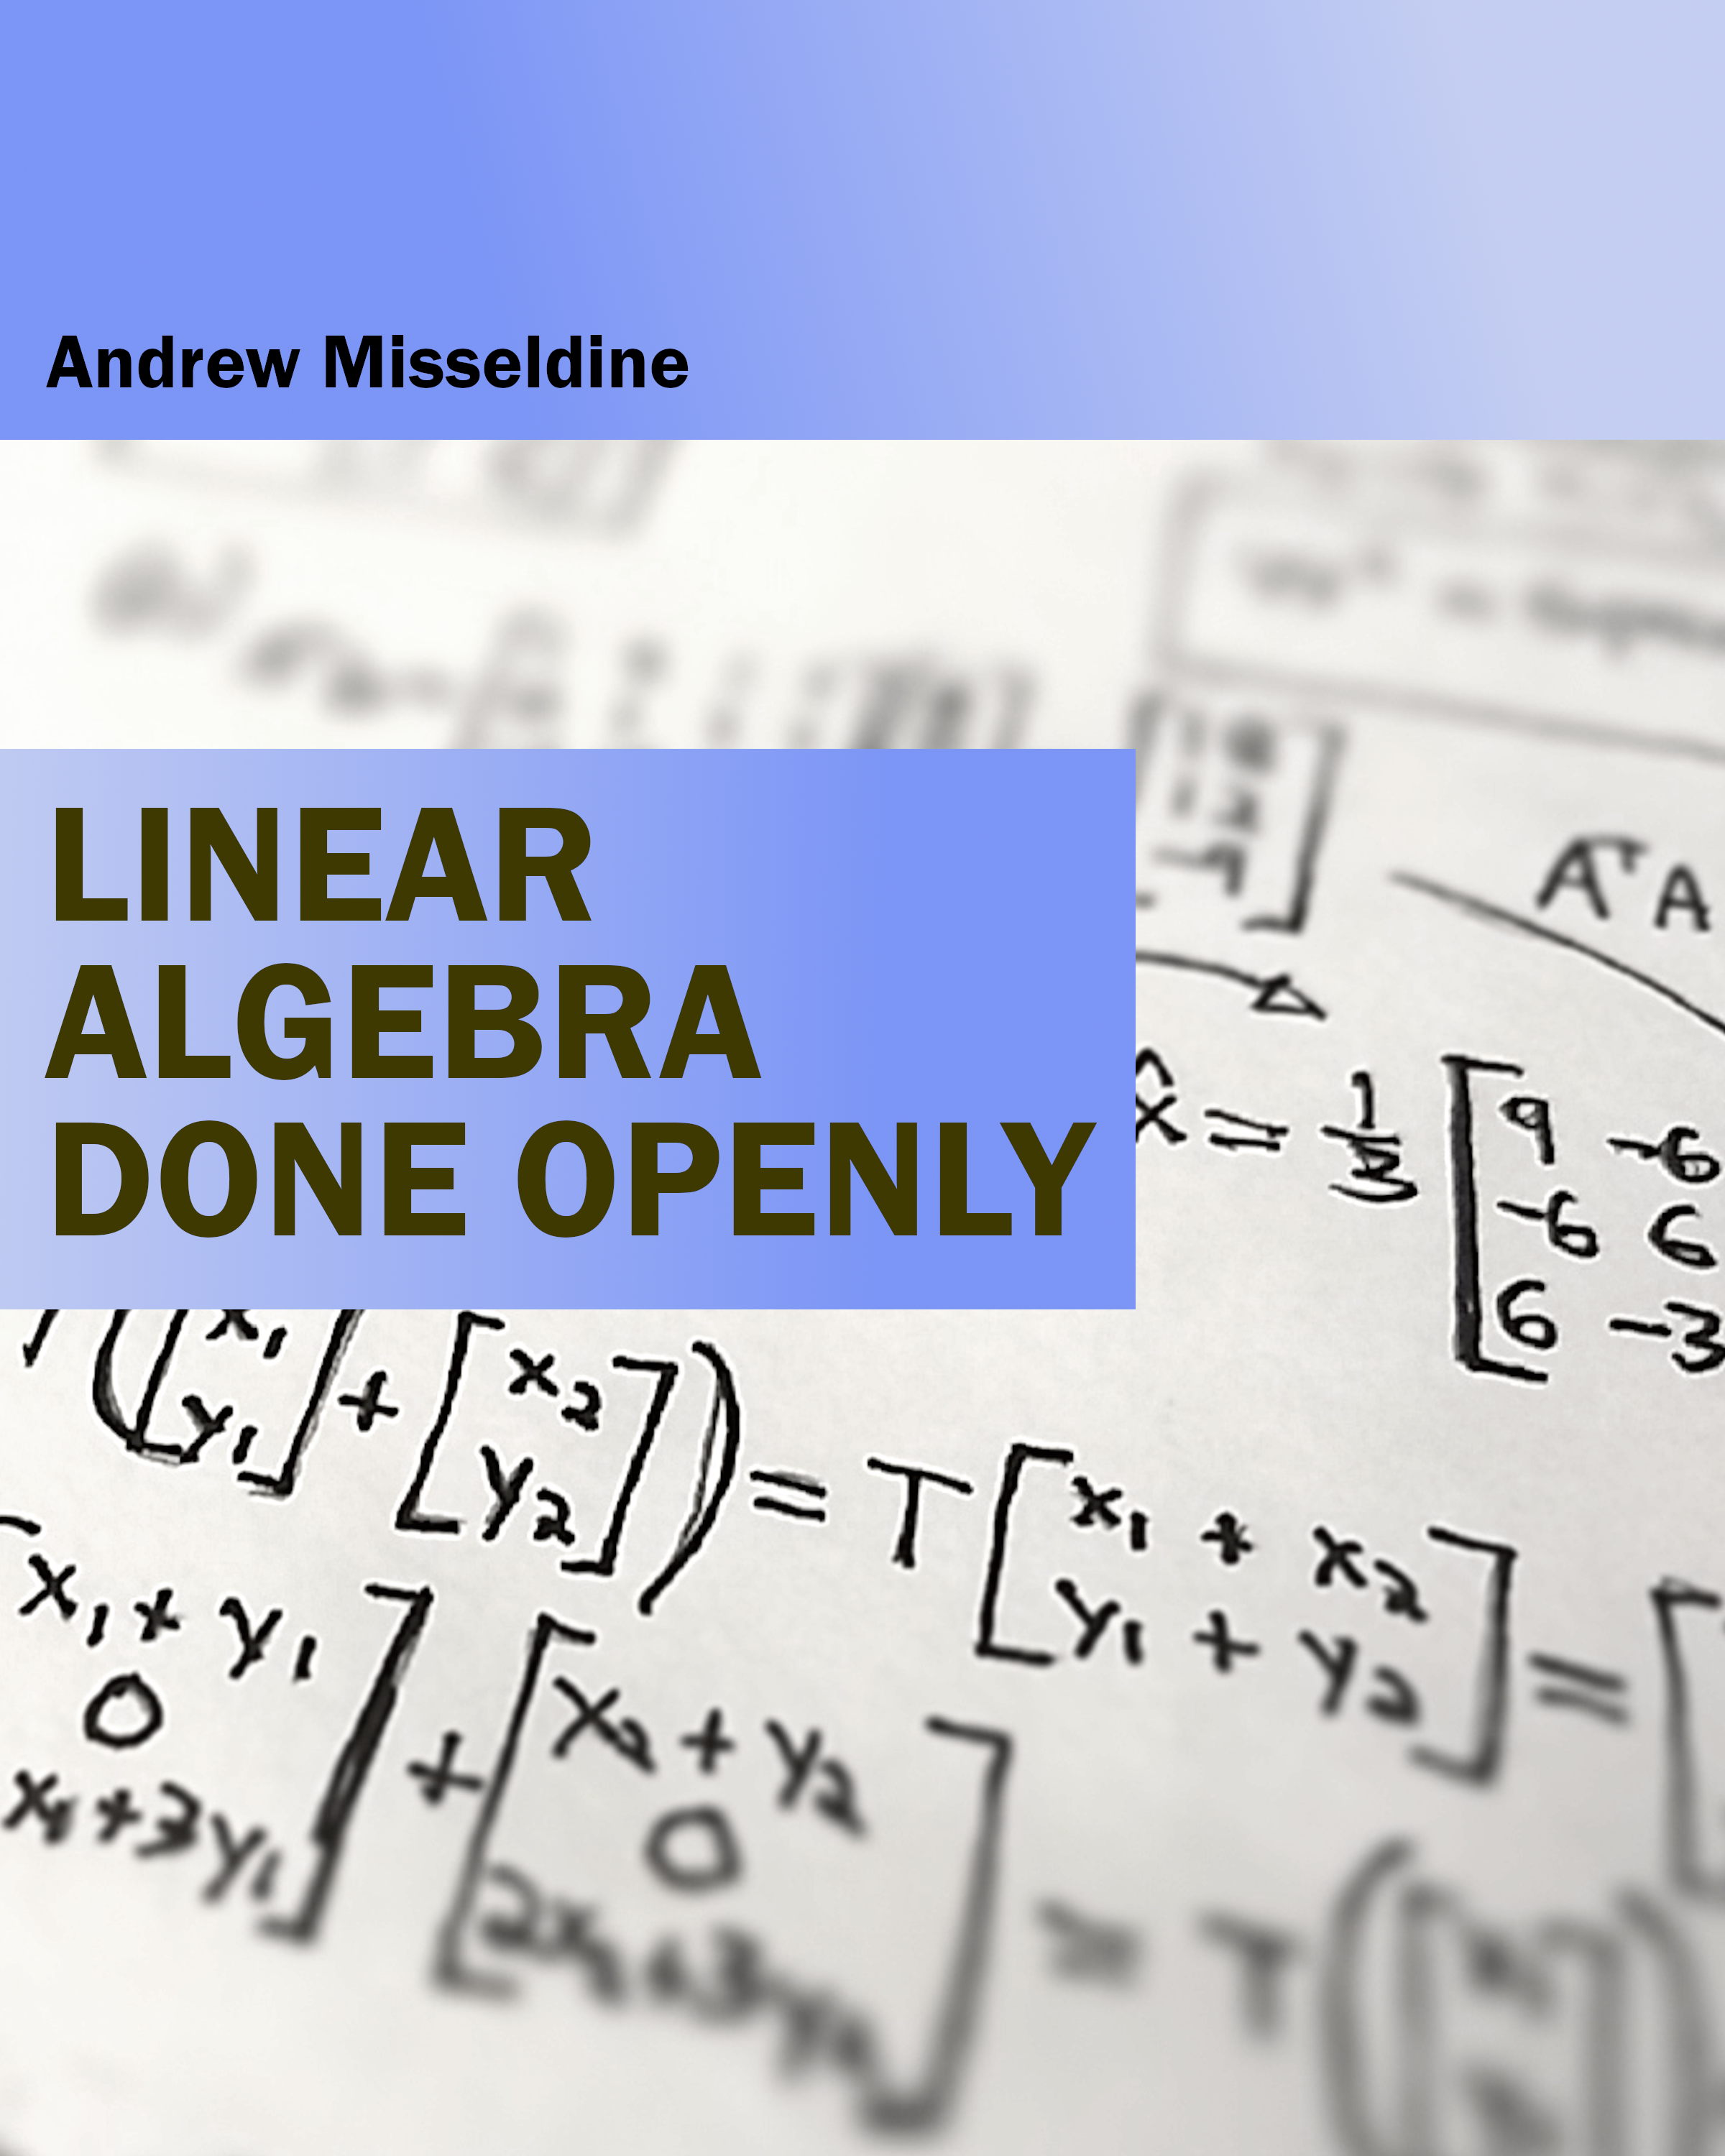
\includegraphics[scale=0.85]{FrontMatter/cover.png}%Daven Triplett
\end{center}
% \pagebreak
% \mbox{}\vfill
% {\vspace{-10 pt}\hfill\footnotesize (Cover contributed by Daven Triplett)}\\ 

\title{Linear Algebra Done Openly}
\author{Andrew Misseldine}
\date{\today}
\maketitle

\pdfbookmark{Table of Contents}{toc}
\tableofcontents


\chapter*{Preface}
\addcontentsline{toc}{chapter}{Preface}

\section*{List of Contributors}
\begin{multicols}{5}
\noindent 
{\footnotesize
Kory Adams\\
Abby Allen\\
Will Allen\\
Kaden Allred\\
%%Akhil Anand\\
Samuel Andersen\\
Caroline Ashton\\
Alicyn Astle\\
Sherie Ayag\\
%Carl Anderson\\
%%Cody Murdock\\
Shelby Bartlett\\
Tyler Bayn\\
Landry Benimana\\
%Matthew Bennion\\
Andrew Biskey\\
Carson Blickenstaff\\
Alexis Borell\\
%Louis Calandrino\\
Braden Carlson\\
Hailey Checketts\\
%%Bo Chen\\
%%Yiyang Chen\\
%%Trevor Cheney\\
Skyler Clark\\
Mariah Clayson\\
%Brett Clouse\\
Cameron Dix\\
Kaylee Dockter\\
Riley Drishinski\\
Joshua Edgel\\
Kaden Empey\\
Candance Fehr\\
Courtney Flanigan\\
Jaren Frandsen\\
C.J. Giacoletto\\
Phillip Goins\\
Jaimie Goldberg\\
Caleb Goodrich\\
Jordan Griffith\\
%%Aramis Hahne\\
Kaylee Hall\\
Malcolm Hanks\\
Thayne Hansen\\
%Andrew Hatch\\
Yingjie He\\
%%Emily Heaton\\%
Bridger Hildreth\\
Christopher Houston\\
Ethan Hoyer\\
%Greyson Hulet\\
Jacob Jensen\\
Sofia Jones\\
Cyrus Kaveh\\
Jacob Kuhn\\
Maria Langford\\
%%Leonid Laykam\\
Laura Lee\\
Yucheng Long\\
%Nick Mackay\\
Jaxton Maez\\
Adam Maxwell\\
%Emily McGee\\
Ellie McReaken\\
%Craig Montgomery\\
Kalvin Mudrow\\
Jacob Newey\\
Christopher Newton\\
Anthony Nguyen\\
Yinglong Niu\\
Gordon Ochsner\\
Brittany Palmer\\
Seth Palmer\\
Darby Parise\\
%Mark Rau\\
Colin Reid\\
Zach Rogers\\
Rindy Roos\\
Hamza Samha\\
Lucas Shaner\\
Hannah Simonson\\
Noah Swenson\\
Ashley Taylor\\
Jaden Torgerson\\
Daven Triplett\\
Runtian Tu\\
Allyson Vest\\
Grayson Walker\\
Gregory Walsh\\
Sarah Walters\\
Adym Warhurst\\
%%Devin Warner\\
Leon Weingartner\\
%%Nathan Wiggins\\
Sarah Wilcox\\
Walt Williams\\
Chance Witt\\
Kyle Wood\\
Kennedy Worthington\\
Jiazheng Yan\\
Jianhe Yu\\
Mattie Zeigler\\
Yifan Zhu\\
Heming Zu\\
Mitchell Zufelt\\
}\end{multicols}
\pagebreak


%Preface Solutions to exercise in back. spade exercises assigned. links for vocab in exercises and sections


\mainmatter
%%%% Chapter 1 %%%%%% 
%Clean, 
\chapter{Introduction to Linear Algebra}\label{chap:linear}

In this first chapter, we want to introduce all the major players in the linear arena. Linear Algebra is the study of \emph{linear} objects (a term we are not quite ready to define). As we have seen linear objects already many times in algebra and calculus, Linear Algebra will take a detailed look at linear structures and this first chapter will explore the important fundamentals of the linear universe.\\

Please be aware that this first chapter may feel awkward or difficult when you read it for the first time. This is both expected and intentional. If you were familiar with all the ideas behind Linear Algebra then you probably would not be reading this book. The struggle herein will produce questions, all of which we will answer in later chapters. Consider this chapter your baptism by fire into all things linear.


\begin{center}
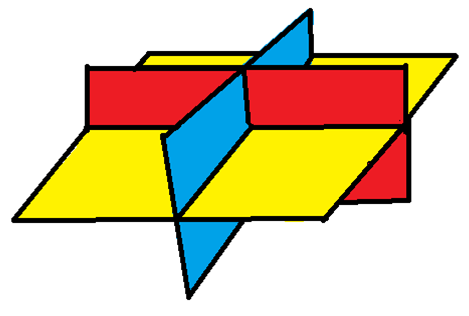
\includegraphics[scale=1]{Chapter1/images/Chapter1cover.png}%Kalvin Mudrow
\end{center}
%{\vspace{-10 pt}\hfill\footnotesize (Image contributed by Kalvin Mudrow)}\\ 

\pagebreak%Introduction to Linear Algebra
\begin{center} 
\emph{``Education is that whole system of human training within and without the school house walls, which molds and develops men.'' -- W. E. B. Du Bois}
\end{center}

\section{Linear Systems}\label{sec:linearsystems}
%\setcounter{Thm}{8}
\setlength{\columnsep}{40pt}
%\renewcommand{\arraystretch}{2.}
\emph{In this section, we introduce the study of linear systems motivated by geometry. Thus, all numbers in this section will be real numbers. We introduce the notion of a system of linear equations and the nature of their solution sets. We discuss when a linear system is consistent/inconsistent, independent/dependent, underdetermined/overdetermined, and homogeneous/nonhomogeneous. We discuss the difference between free and dependent variables in a linear system.}

\begin{Def}\label{def:linearsystem} A \textbf{system of linear equations}\index{linear system} (or a \textbf{linear system}) is a set of equations with common variables of the following form:
\[a_1x_1+a_2x_2+\ldots+a_nx_n = b,\] where $b$ and the \textbf{coefficients} $a_1, \ldots, a_n$ are fixed numbers.\\

 A \textbf{solution} to a system is an assignment to each variable such that each equation is satisfied. The \textbf{solution set} is the set of all solutions to a system of equations. Two systems of equations are \textbf{equivalent} if they have the same solution set.
\end{Def}

A linear equation of two real variables (typically $x, y$ or $x_1, x_2$) geometrically forms a \emph{line} in the plane. Likewise, a linear equation of three real variables (typically $x, y, z$ or $x_1, x_2, x_3$) geometrically forms a \emph{plane} in 3-space. Although much harder to visualize, a linear equation in four variables (typically $x, y, z, w$ or $x, y, z, t$ or $x_1, x_2, x_3, x_4$) geometrically forms a \emph{hyperplane} in 4-space. Higher dimensional analogues likewise exist. As such, emphasis in this section will be placed on linear systems with two or three real variables. \\

\begin{multicols}{2}
\begin{Exam}\label{exam:1.1firstgeom} Test that $(3,1)$ is a solution to the system \[\begin{linear} &x\ &+\ &5&y\ &=\ &8& \\ 2&x\ &-\ &&y\ &=\ &5&.  \end{linear}\]   

Notice that $3+ 5(1) = 3+5 = 8$ and $2(3) - 1 = 6 -1 = 5$. Thus, $(3,1)$ is a solution to the above system.\\

Geometrically, the solution to the previous system is an intersection between two lines, as depicted to the right. \vspace{-0.2 in}
\begin{center}
\begin{tikzpicture}[scale= .5]
\draw[<->, very thick] (-5,0) -- (5,0)node[below] {$x$};
\draw[<->, very thick] (0,-2) -- (0,6) node[right] {$y$};

\draw[red, ultra thick, domain = 1.5:5, samples = 400, <->] plot (\x, {2*\x-5}) node[right] {$2x-y=5$};
\draw[blue, ultra thick, domain = -5:5, samples = 400, <->] plot (\x, {-\x/5+8/5}) node[right] {$x+5y=8$};

\draw (4.25,1.35) node {$(3,1)$};
\draw[fill] (3,1) circle (.2);
\end{tikzpicture}
\end{center}
\end{Exam}
\end{multicols}\vs

\begin{Exam} \label{exam:1.1firstthree} Consider the linear system with three variables and three equations: \[\begin{linear} x\ &+\ &2y\ &+\ &3z\ &=\ &20\\ -2x\ &+\ &y\ &&\ &=\ &-1\\ -3x\ &-\ &6y\ &+\ &5z\ &=\ &-4. \end{linear}\] %Mariah Clayson

We can check that $(2,3,4)$ is a solution of this system. Note that $(2) + 2(3) + 3(4) = 2+8+12=20\ \checkmark$, $-2(2) + (3)  = -4+3=-1\ \checkmark$, and $-3(2) - 6(3) + 5(4) = -6-18+20 = -4\ \checkmark$, which shows that $(2,3,4)$ is in fact a solution of the system. Try as one might, another solution to this system CANNOT be found, that is, $(2,3,4)$ is the unique solution to this system of equations.
\end{Exam}

\begin{Exam}\label{exam:1.1dependent} Consider the linear system with three variables and three equations: \[\begin{linear} 2x\ &-\ &y\ &+\ &z\ &=\ &11\\ x\ &+\ &3y\ &-\ &10z\ &=\ &2\\ -3x\ &+\ &2y\ &-\ &3z\ &=\ &-17&. \end{linear}\] %Daven Triplett

It is simple to check that $(5,-1,0)$ is a solution to this system. Likewise, we can also show that $(6,2,1)$ is a solution to this same system. Thus, it is possible to have multiple solutions to a linear solutions.
\end{Exam}\vs

Because of \examref{exam:1.1dependent}, it is worth investigating how many solutions a linear system may have. The beginning of our investigation is the following definitions.\\


\begin{Def}\label{def:consistent} A system of equations is \textbf{consistent} if it has a solution. Otherwise, we call the system \textbf{inconsistent}.\\

If a consistent linear system has a unique solution, we call this the \textbf{independent case}.\label{def:uniquesoln} If a consistent linear system has multiple solutions, we call this the \textbf{dependent case}.\end{Def}\vs

Like we did in \examref{exam:1.1firstgeom}, we will investigate linear systems with two variables and their corresponding geometry.\\

\begin{Exam} Solve each system of equations. 
\begin{enumerate}
\begin{multicols}{2}
\item $\begin{linear} 
5x\ &+\ &2y\ &=\ &32\\
3x\ &+\ &6y\ &=\ &48 
\end{linear}$\\

After graphing the two lines, as depicted to the right, we see that the two lines intersect at a unique point. This point of intersection, \fbox{$(4,6)$}, means the system has a unique solution. Therefore, the system is consistent and independent.\\

\begin{center}
\begin{tikzpicture}[scale = 0.75]
\gridlines{-0.5}{5}{-0.5}{5};
\node[below, yshift= -5] at (1,0) {$1$};
\node[below, yshift= -5] at (2,0) {$2$};
\node[below, yshift= -5] at (3,0) {$3$};
\node[below, yshift= -5] at (4,0) {$4$};
\node[left, xshift= -5] at (0,1) {$5$};
\node[left, xshift= -5] at (0,2) {$10$};
\node[left, xshift= -5] at (0,3) {$15$};
\node[left, xshift= -5] at (0,4) {$20$};

\draw[ultra thick, blue, <->] plot[domain = -0.5:5] ({\x}, {-1/2*\x + 16/5}) node[below right] {$5x+2y=32$};
\draw[ultra thick, red, <->] plot[domain = -0.5:5] ({\x}, {-1/10*\x + 8/5}) node[above right] {$3x+6y=48$};
\fill (4, 6/5) circle (0.15) node[below left] {$(4,6)$};
\end{tikzpicture}
\end{center}
\end{multicols}

\begin{multicols}{2}
\item $\begin{linear} 
&&y\ &=\ &-x\ &+\ &5\\
2x\ &+\ &2y\ &=\ &3 
\end{linear}$\\

After graphing the two lines, as depicted to the right, we see that the two lines are parallel. Thus, they do NOT ever intersect. Therefore, the system is \fbox{inconsisitent}, that is, there is no solution to the linear system.\vfill

\begin{center}
\begin{tikzpicture}[scale = 0.75]
\gridlines{-2}{2}{-1}{7};

\draw[ultra thick, blue, <->] plot[domain = -2:2] ({\x}, {-\x+5}) node[below right] {$y=-x+5$};
\draw[ultra thick, red, <->] plot[domain = -2:2] ({\x}, {-\x+1.5}) node[below right] {$2x+2y=3$};
\end{tikzpicture}
\end{center}
\end{multicols}
\pagebreak
\begin{multicols}{2}
\item $\begin{linear} 
&&x\ &=\ &\dfrac{2}{3}y\ &+\ &3\\
3x\ &-\ &3y\ &=\ &9 
\end{linear}$\\

After graphing the two lines, as depicted to the right, we see that the two lines are the same line. Thus, every point on one line is also a point on the other line. Therefore, the system is dependent, that is, there are infinitely many solutions to the linear system. In particular, the system is consistent.\vfill

\begin{center}
\begin{tikzpicture}[scale = 0.75]
\gridlines{-1}{6}{-3}{3};

\draw[ultra thick, blue, <->] plot[domain = -3:3] ({2/3*\x+3}, {\x}) node[below right] {$x=\dfrac{2}{3}y+3$};
\draw[ultra thick, dashed, red, <->] plot[domain = -3:3] ({2/3*\x+3}, {\x}) node[left, xshift=-3] {$3x-3y=9$};
\end{tikzpicture}\hfill$\qedhere$
\end{center}
\end{multicols}

\end{enumerate}
\end{Exam}

In general, any two lines in the real plane intersect at  0, 1, or infinitely many points (this last case occurs if the lines overlap). This holds also for higher dimensional systems of linear equations, that is, for any system of linear real equations the number of solutions is 0, 1, or $\infty$ and the solution set of a linear system will fall under one of these three types.\\

 These three possibilities are also the case for intersections of planes in 3-dimensional space. The \hyperref[def:consistent]{\emph{independent, consistent}} case occurs when all planes in the system intersect at a unique point. This was the case for \examref{exam:1.1firstthree}. Visually, this can be seen as three planes intersecting at a unique point, such as the three planes involved in \examref{exam:1.1firstthree}, illustrated below:
\begin{center} 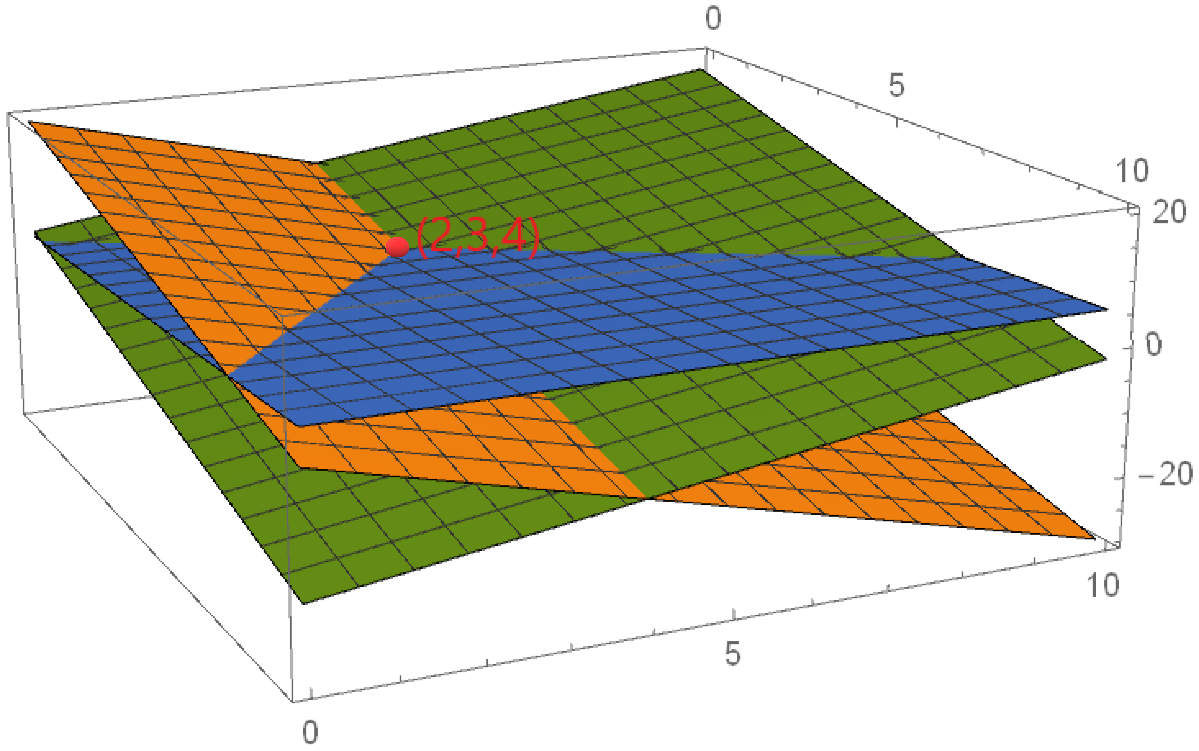
\includegraphics[scale=.25]{Chapter1/images/1-1firstthree.png} \end{center}%Mariah Clayson
The \hyperref[def:consistent]{\emph{inconsistent}} case occurs when not all the planes simultaneously intersect at a common point, perhaps because some subset of planes are parallel with one another. Finally, the \hyperref[def:consistent]{\emph{dependent, consistent}} case occurs when the collection of planes overlay at more than one point, e.g. three planes in 3-space intersect along a common line, as illustrated below: 
\begin{center} 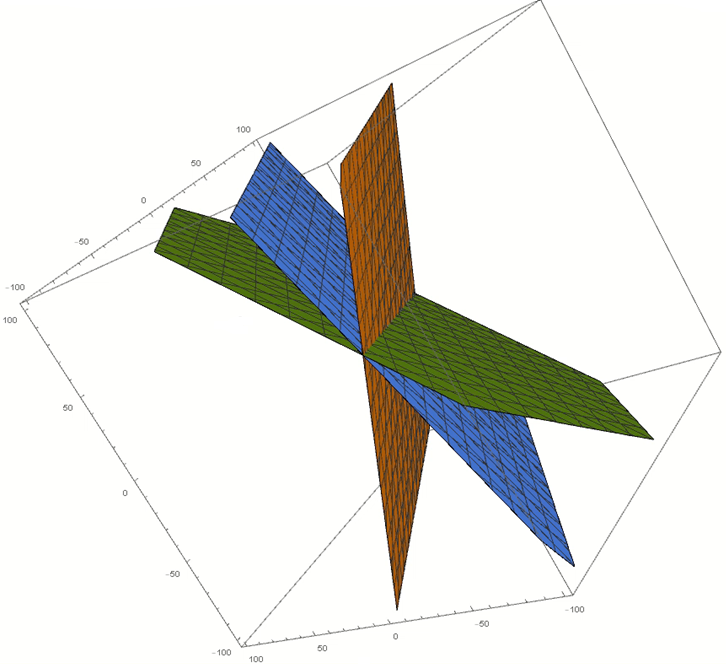
\includegraphics[scale=.35]{Chapter1/images/1-1secondthree.png} \end{center}%Greg Walsh 
This was the case for \examref{exam:1.1dependent}. In fact, any point of the form 
\setcounter{equation}{\value{Thm}} \begin{equation}\label{exam:generalform} (z+5, 3z-1,z), \end{equation} \stepcounter{Thm}
 where the variable $z$ can be freely assigned to any real number, is a solution to this linear system. This is called the \textbf{general solution} to the system. In this example, $z$ is a \mbox{\label{def:freevar}\textbf{free variable},} that is, a variable which can be assigned any value. The other two variables, $x$ and $y$, are called \textbf{dependent variables}, because their assignment is dependent upon the assignments of the free variables corresponding to some linear relationship. Thus, the linear system in \examref{exam:1.1dependent} has one free variable and two dependent variables. The two solutions listed in \examref{exam:1.1dependent} arose exactly from setting $z=0$ and $z=1$, respectively. In general, the dependent case occurs exactly when the linear system has at least one free variable. \\

The following properties will be proven in the homework.\\

\begin{Prop} \label{prop:1.1determine} Suppose that a consistent linear system has $m$ equations and $n$ variables. 
\begin{enumerate}[label=(\roman*), series=!THM!]
\item  If $n > m$, then the system has at least $n-m$ free variables which implies that it has multiple solutions.\\
\item If $m > n$, then the system has at least $m-n$ many equations which could be removed without modifying the solution set.
\end{enumerate}
\end{Prop}\vs

The situation where $n >m$ is called an \textbf{underdetermined system} because there are not enough equations to guarantee a unique solution. The situation where $m >n$ is called an \textbf{overdetermined system} because there might be too many equations to guarantee consistency. 

\begin{Def}\label{def:homogeneous} A system of linear equations is called \textbf{homogeneous} if each equation is of the form:
\[a_1x_1+a_2x_2+\ldots+a_nx_n = 0.\] Otherwise, the system is called \textbf{nonhomogeneous}.\\
\end{Def}


\begin{Exam}  The below $3\times 3$ linear system is homogeneous since the right hand side of each equation is 0: %Seth Palmer
\[\begin{linear} x\ &+\ &3y\ &+\ &5z\ &=\ &0\\
2x\ &+\ &4y\ &+\ &6z\ &=\ &0\\
4x\ &+\ &2y\ & & &=\ &0
\end{linear}\]

On the other hand, the below linear system appears to be homogeneous at first, but is really non-homogeneous: %Malcolm Hanks
\[\begin{linear} x\ &+\ &3y\ &-\ &2z\ &+\ &4\ &=\ &0\\
4x\ &+\ &2y\ &+\ &3z\ &-\ &5\ &=\ &0\\
-x\ &+\ &5y\ &-\ &3z\ &-\ &2\ &=\ &0
\end{linear}\] The issue here is that the linear system is not in \emph{standard form}, that is, all the variables are located on the left-hand sides of the equations, in descending order, and the constants are all on the right-hand sides of the equations. In standard form, the system would appear as:
\[\begin{linear} x\ &+\ &3y\ &-\ &2z\ &=\ &-4\\
4x\ &+\ &2y\ &+\ &3z\ &=\ &5\\
-x\ &+\ &5y\ &-\ &3z\ &=\ &2&0
\end{linear}\] In standard form, it is much more clear that the above linear system is non-homogeneous.
\end{Exam}\vs

\begin{Prop}\label{prop:1.1homo} A homogeneous system of equations is always consistent. \end{Prop}

%%%%%%%%%%%%%%%%%%% Exercises %%%%%%%%%%%%%%%%%%%
\startExercises{linearsystems}

\noindent For Exercises \ref{exer:checksolutionsecondstart}--\ref{exer:checksolutionsecondstop}, determine if the point is a \hyperref[def:linearsystem]{solution to the following linear system}\\  $\begin{linear} x\ &+\ &y\ &&&=\ &7\\ 3x\ &+\ &3y\ &-\ &10z\ &=\ &-79\\ x\ &+\ &5y\ &+\ &z\ &=\ &33&.\end{linear}$  %Cameron Dix
\begin{multicols}{4}
\begin{enumerate}[series=!HW!, label=\arabic*., ref=\arabic*]
\item \label{exer:checksolutionsecondstart} $(4,3,10)$ 
\item $(0,0,0)$
\item $(3,4,10)$
\item\label{exer:checksolutionsecondstop} $(-10,3,-38)$
\end{enumerate}
\end{multicols}\vs

\noindent For Exercises \ref{exer:checksolutionfirststart}--\ref{exer:checksolutionfirststop}, determine if the point is a \hyperref[def:linearsystem]{solution to the following linear system}\\ $\begin{linear} x\ &+\ & 3y\ &-\ &2z\ &=\ &13\\ 2x\ &-\ &y\ &&&=\ &2\\ -x&+\ &6y\ &-\ &4z\ &=\ &17&.\end{linear}$   %Abby Allen
\begin{multicols}{4}
\begin{enumerate}[!HW!, label=$\spadesuit$ \arabic*., ref=\arabic*]
\item\label{exer:checksolutionfirststart} $(6,10,4)$
\item $(5,8,8)$ 
\item $(3,4,1)$
\item \label{exer:checksolutionfirststop} $(9,3,2)$
\end{enumerate}
\end{multicols}\vs


\noindent For Exercises  \ref{exer:checksolutionthirdstart}--\ref{exer:checksolutionthirdstop}, determine if the point is a \hyperref[def:linearsystem]{solution to the following linear system}\\ $\begin{linear} x\ &-\ & y\ &+\ &z\ &=\ &5\\ 3x\ &+\ &4y\ &-\ &5z\ &=\ &-2\\ -2x&-\ &4y\ &+\ &7z\ &=\ &11&.\end{linear}$   %anon
\begin{multicols}{5}
\begin{enumerate}[!HW!]
\item\label{exer:checksolutionthirdstart} $(1,2,3)$
\item $(3,2,1)$ 
\item $(5,0,6)$
\item $(3,1,3)$
\item \label{exer:checksolutionthirdstop} $(9,3,2)$
\end{enumerate}
\end{multicols}\vs

\noindent For Exercises \ref{exer:dependentsystemstart}--\ref{exer:dependentsystemstop}, graph the \hyperref[def:linearsystem]{linear system} and determine if it is \hyperref[def:consistent]{consistent or inconsistent}. If consistent, determine which whether it has a \hyperref[def:uniquesoln]{unique solution or multiple solutions}.
\begin{enumerate}[!HW!]
\begin{multicols}{3}
\item\label{exer:dependentsystemstart}  $\begin{linear} 14x\ &+\ &3y\ &=\ & 4\\ 5x\ &+\ &9y\ &=\ &1 \end{linear}$ %Hannah Simonson
\item $\begin{linear}
2x\ &-\ &5y\ &=\ &10\\ \frac{4}{5}x\ &-\ &2y\ &=\ &4
\end{linear}$ %Christopher Newton
\item $\begin{linear} x\ &=\ & 5y\ &-\ &4\\ \frac{1}{5}x\ &=\ &y\ &+\ &13 \end{linear}$ %Hannah Simonson
\end{multicols}
\begin{multicols}{3}
\item $\begin{linear} 2x\ &+\ &3y\ &=\ &4\\ x\ &-\ &y\ &=\ &2 \end{linear}$ %Jacob Newey
\item $\begin{linear} -4x\ &+\ &y\ &=\ &7\\ -8x\ &+\ &2y\ &=\ &2 \end{linear}$ %Jacob Newey
\item $\begin{linear} x&\ -\ &y\ &=\ &1\\ 2y\ &=\ &2x\ &-\ & 2\end{linear}$ %Jacob Newey
\end{multicols}
\begin{multicols}{3}
\item $\begin{linear} y\ &=\ &2x\ &+\ &7\\ y\ &=\ &-4x\ &-\ &2 \end{linear}$ %Ellie McReaken
\item $\begin{linear} &&&&y\ &=\ &5x\ &+\ &8\\ -5x\ &+\ &y\ &-\ &2\ &=\ &6\end{linear}$ \\%Ellie McReaken
\item $\begin{linear} &&y\ &=\ &3x\ &-\ &7 \\ y\ &-\ &3x\ &=\ &12\\ \end{linear}$ %Ellie McReaken
\end{multicols}
\begin{multicols}{3}
\item\label{exer:dependentsystemstop} $\begin{linear}9x\ &+\ &5\ &=\ &2y\\ x\ &+\ &2y\ &=\ &5\\ &&y\ &=\ &2.5 \end{linear}$ %Hannah Simonson
\end{multicols}
\end{enumerate}\vs

\noindent For Exercises \ref{exer:homogeneoussystemstart}--\ref{exer:homogeneoussystemstop}, determine if the \hyperref[def:linearsystem]{linear system} is \hyperref[def:homogeneous]{homogeneous}. For those which are, find a \hyperref[def:linearsystem]{solution}. 
\begin{enumerate}[!HW!]
\begin{multicols}{3}
\item\label{exer:homogeneoussystemstart} $\begin{linear} 4x\ &+\ &2y\ &=\ &0\\ 5x\ &+\ &3y\ &=\ &0\end{linear}$ %Yinglong Niu
\item $\begin{linear} 6x\ &-\ &7y\ &=\ &3\\ 2x\ &+\ &8y\ &=\ &0\end{linear}$ %Yinglong Niu
\itemspade $\begin{linear} 3x\ &-\ &y\ &=\ &0 \\ 2x\ &+\ &5y\ &=\ &0 \end{linear}$ %Lucas Shaner
 \end{multicols}
\begin{multicols}{3}
 \itemspade $\begin{linear} 2x\ &-\ &4y\ &=\ &0\\ -6x\ &+\ &8y\ &=\ &3 \end{linear}$ %Lucas Shaner
 \item $\begin{linear} -5\ &-\ &y\ &-\ &2\ &=\ &0 \\ x\ &+\ &y\ &+\ &5\ &=\ &0 \end{linear}$ %Lucas Shaner
  \item $\begin{linear} 2x\ &+\ &y\ &=\ &10\\ -7x\ &-\ &3y\ &=\ &3 \end{linear}$ %Lucas Shaner
 \end{multicols}
\begin{multicols}{3}
\item $\begin{linear} 5x\ &+\ &2y\ &+\ &3z\ &=\ &2\\ 3x\ & & &-\ &4z\ &=\ &-1\\  & &5y\ &+\ &3z\ &=\ &5
\end{linear}$ %Yinglong Niu
 \item $\begin{linear} 5x\ &+\ &2y\ &+\ &3z\ &=\ &2\\ -3x\ &-\ &2y\ &+\ &z\ &=\ &5\\ 2x\ &+\ &2y\ &-\ &4z\ &=\ &1 \end{linear}$ %Daven Triplett
\itemspade $\begin{linear} x\ &&&-\ &2z\ &&&=\ &0\\ 3x\ &+\ &4y\ &+\ &4z\ &+\ &w\ &=\ &0\\ -2x\ &+\ &6y\ &+\ &6z\ &+\ &2w\ &=\ &0 \end{linear}$ %Daven Triplett
 \end{multicols}
\begin{multicols}{3}
\item\label{exer:homogeneoussystemstop} $\begin{linear} 2x\ &-\ &2y\ &-\ &2z\ &=\ &6\\ -x\ &-\ &3y\ &+\ &9z\ &=\ &1\\ 4x\ &+\ &3y\ &-\ &18z\ &=\ &3 \end{linear}$ %Daven Triplett
 \end{multicols}
 \end{enumerate}\vs
 
\begin{enumerate}[!HW!]
\item\label{exer:homogeneoussystemhint} Is the \hyperref[def:linearsystem]{linear system} $\begin{linear} x\ &+\ &2y\ &-\ &4z\ &=\ &0\\ &&-y\ &+\ &3z\ &=\ &0\\ 2x\ &+\ &3y\ &&&=\ &0\end{linear}$ \hyperref[def:consistent]{consistent}? Why or why not? Draw a 3-dimensional sketch of these planes and their intersection.  %Jacob Newey

\itemspade Using the \hyperref[exam:generalform]{general form} for \examref{exam:1.1dependent} provided on page \pageref{exam:generalform} (namely \eqref{exam:generalform}), construct five other solutions to the \hyperref[def:linearsystem]{linear system} from \examref{exam:1.1dependent}. Answers may vary.

\itemspade Prove \propref{prop:1.1homo}.
\end{enumerate}

%%%%%%%%%%%%%%%%%%% Footnotes

%%%%%%%%%%%%%%%%%%%
\pagebreak%1.1 Linear Systems
\begin{center} 
\emph{``Hold fast to dreams\ldots For when dreams go\\ Life is a barren field\ldots Frozen with snow.'' -- Langston Hughes}
\end{center}

\section{Fields}\label{sec:fields}
The topic of this section will be about what is even a number. This discussion is often postponed to more advanced mathematics courses where abstraction is king, but for linear algebra students, this abstraction is just budding. This course will be primarily a computational introduction to linear algebra with select proofs and applications. In spite of this goal, the abstract notion of a field will not hinder this. In fact, the introduction of various fields will strengthen the student's understanding of the concepts and computations of linear algebra as the student will see what parts are truly necessary and when variability is allowed. This will also strengthen the realization that discussion of complex vector spaces and real vector spaces are not two separate discussion but instead one same story.\\

What really is a number? Although numbers are useful for counting, they are much more useful than that.  A simple answer would be to say it is a thing with which we do math on. Although a crude response, this will satisfy our inquiry, thus avoiding a long journey through deep logic and philosophy. Maybe another day.\\

%%%%%%%%%%%%%%%%%%%MOVE TO APPENDIX%%%%%%%%%%%%%%%%%%%%%%%%%%%%%%%%%
A \textbf{set} to us will mean a collection of objects, typically called \textbf{elements}. Those elements could be numbers, colors, people, pok\'{e}mon, or other sets! Typically, sets will be denoted by capital alphabet letters such as $A$, $B$, $C$, etc. and elements with lower case letters such as $a$, $b$, $c$, etc. Typically, $\{\ldots\}$ is used to denote the elements in a set, i.e. $A=\{1, 2, 3, 4\}$. Often a set is described by some rule, such as $A = \{x\mid \text{x satisfies some rule}\}$. If an element $x$ is a member of the set $X$, then we denote this as $x\in A$. Then notation $x\notin A$ means that $x$ is not an element of $A$. There must be a clear rule to decide whether an element is a member of a set or not, otherwise it is not a set. The set which contains no elements, $\emptyset = \{\}$, is called the \textbf{empty set}.\\

A \textbf{function} $f$ is a relationship between sets, say $A$ and $B$, such that each element of $A$ is assigned to exactly one element of $B$ (although not all elements of $B$ must be assigned to an element of $A$). We denote this function relation as $f : A\to B$. If $A$ and $B$ are two sets, we let $A\times B$ denote the set of ordered pairs of elements from $A$ and $B$. For example, if $a\in A$ and $b\in B$, then $(a,b)\in A\times B$. Finally, an \textbf{operation} is a function of the form $f : A\times B \to C$. One should think of an operation as a process of bringing two objects together and creating a third object.\\
%%%%%%%%%%%%%%%%%%%MOVE TO APPENDIX%%%%%%%%%%%%%%%%%%%%%%%%%%%%%%%%%

\subsection{Fields}
 We are now ready for the definition of a field of numbers. Do not panic. If this seems very fast, that is okay. Our discussion will slow down quickly.\\

\begin{Def}\label{def:field} A \textbf{field} is a nonempty set $F$ with elements called \textbf{scalars} on which are defined two operations, called \textbf{addition} $+ : F\times F \to F$ and \textbf{multiplication} $\cdot : F\times F \to F$, such that for all scalars $a, b, c \in F$, the following ten axioms hold:
\setlength{\columnsep}{30pt}
\begin{multicols}{2}
\begin{enumerate}[label=\emph{(\roman*)}, series=!DEF!]
\item\label{ax:addcom} $a+b=b+a$ 
\item\label{ax:addass} $(a+b)+c=a+(b+c)$ 
\item\label{ax:addid} There exists  a scalar $0\in F$, such that\\ $a + 0 = 0 + a = a$ 
\item\label{ax:addinv} For each $a$, there exists a scalar $-a \in F$, such that $a + (-a) = (-a) + a = 0$ 
\item $a\cdot (b+c) = (a b) + (a c)$\columnbreak
\item\label{ax:multcom} $ab=b a$ 
\item\label{ax:multass} $(a b)c=a(b c)$ 
\item\label{ax:multid} There exists  a scalar $1\in F$, such that\\ $a  1 = 1  a = a$ 
\item\label{ax:multinv} For each $a\neq 0$, there exists a scalar $a^{-1} \in F$, such that $a  a^{-1} = a^{-1}  a = 1$ 
\item $(a+b)\cdot c = (a c) + (b c)$
\end{enumerate}
\end{multicols}
\end{Def}

It might seem like a daunting list but remember the following: a field is just a number system for which we can add, subtract, multiply, and divide following the usual commutative, associative, and distributive laws. The set of rational numbers, denoted $\Q$, is a field. The set of real numbers $\R$ and the set of complex numbers $\C$ are also both fields. These are the fields that we are most familiar with. Note that the set of integers $\Z$ is NOT a field, as the quotient of two integers is not always an integer, e.g. $\dfrac{1}{2}\notin \Z$. Likewise, the set of natural numbers $\N$ is NOT a field for the same reasons with division but also because the difference of two natural numbers is not always a natural number, e.g. $3-4 = -1 \notin \N$.\\

Fields are the number systems we are used to in previous algebra classes. For example, fields are exactly the environment where linear equations can be solved. Let $F$ be a field and $ax+b=c$ is a linear equation\label{note:lineareqn} with variable $x$ and $a,b,c\in F$. Here the variable itself is a placeholder for some other scalar. A \textbf{solution} to this linear equation is an assignment to the variable $x$ which makes the equation true. For linear equations, we see there is only one solution in any field:
\begin{align*}
ax+b&=c&\\
(ax+b)+(-b)&=c+(-b)& \text{Existence of Additive Inverses \eqref{ax:addinv}}\\
ax+(b-b)&=c-b& \text{Additive Associativity \eqref{ax:addass}}\\
ax+0&=c-b& \\
ax&=c-b& \text{Existence of Additive Identity \eqref{ax:addid}}\\
a^{-1}(ax)&=a^{-1}(c-b)& \text{Existence of Multiplicative Inverses \eqref{ax:multinv}}\\
(a^{-1}a)x&=\dfrac{c-b}{a}& \text{Multicative Associativity \eqref{ax:multass}}\\
1x&=\dfrac{c-b}{a}& \\
x&=\dfrac{c-b}{a}& \text{Existence of Multicative Identity \eqref{ax:multid}}\\
\end{align*}

Note that commutativity is used to guarantee that subtraction and division is well-defined. Therefore, a linear equation has a unique solution over a field.\\

\begin{Exam} Solve the following equations:
\begin{enumerate}
\item $2x+1=6$ over $\Q$\\
\[2x+1=6 \qRightarrow 2x = 6-1=5 \qRightarrow x = \fbox{$\dfrac{5}{2}$}.\]

\item $(i+1)x + (3-i) = 4+5i$ over $\C$\\
\[ (i+1)x + (3-i) = 4+5i \qRightarrow (i+1)x = (4+5i) - (3-i) = 1+6i\]\[ \qRightarrow x = \dfrac{1+6i}{1+i} = \dfrac{1+6i}{1+i}\left(\dfrac{1-i}{1-i}\right) = \dfrac{1-i+6i+6}{1-i+i+1} = \fbox{$\dfrac{7}{2} + \dfrac{5}{2}i$}.\qedhere\]
\end{enumerate}
\end{Exam}\vs


\subsection{Modular Arithmetic and Finite Fields}
We introduce now one last type of field: a finite field. Let $n$ be a positive integer and let $a$ be any integer. Consider the operation $a\div n$. The division algorithm known unto us since primary school guarantees there are unique integers $q, r$, called the \emph{quotient} and \emph{remainder}, respectively, such that $a=qn+r$ where $0\le r< n$. For example, for $n=5$ and $a=13$, we have that $13=2(5) + 3$, that is, $q=2$ and $r=3$. We generally would interpret this statement as $5$ divides into $13$ two times with remainder of three, that is, if $13$ vectors are to be shared among $5$ friends then each friend would get $2$ vectors with $3$ vectors left over. Typically, with a division problem one is interested in finding the quotient but in \textbf{modular arithmetic}, one is instead interested in finding the remainder, which has many powerful uses. Let $\Z_n = \{0, 1, 2, \ldots, n-1\}$. Then $\Z_n$ should be viewed as the set of all possible remainders, or \textbf{residues}, when divided by $n$. Define next a function $\pmod n : \Z \to \Z_n$ by the rule $a \pmod n$ is the unique remainder of $a$ when divided by $n$. For example, $8 \pmod 5 = 3$. Likewise, $14\pmod 5 = 4$ since $14=2(5)+4$, that is, $5$ divides into $14$ twice with a remainder of $4$. The residue $a\pmod n$ is read "$a$ modulo $n$" and $n$ is called \textbf{modulus} of the function.\\

Note that if $0\le a < n$, then $a\pmod n = a$, the original value, for example, $3\pmod 5 = 3$. In this example, the associated quotient is $0$. This is a department from decimal division where the fraction $\frac{3}{5}$ may be expressed as the decimal $0.6$. Special attention should also be given to when $a$ is a negative integer. Note that $-11 \pmod 6 = 1$ since $-11 = (-2)(6) + 1$, where the quotient is $-2$ and the residue is $1$. This is in contrast to the possibility $-11 = (-1)(6) + (-5)$. The difference here is that while quotients may be any integer: positive, zero, or negative, remainder must always exist in the range $0\le r \le n-1$, which is necessarily nonnegative. \\

When $a\ge n$, one way to determine $a\pmod n$ is to subtract from $a$ the modulus $n$ until the difference lies in $\Z_n$. For example, $14>5$, the first difference $14-(1)5 =14-5=  9$ is still too large. The second difference $14-2(5) = 9-5 = 4\in \Z_5$. Thus, $14\pmod 5=4$, as observed above. This notion of repeated subtraction is actually where the division algorithm gets its life, in a similar way of viewing multiplication as repeated addition. When $a$ is negative, we can instead add the modulus $n$ to $a$ (or subtract a negative, if one prefers) until the sum lies inside of $\Z_n$. For examples, $-11-(-1)6=-11+6= -5$ which is too small, but the next iteration $-11-(-2)6 = -5+6 = 1$. Thus, $-11\pmod 6=1$, as observed above. \\

Note that $7\pmod 6 = 1 = -11 \pmod 6$, that is, it is possible for two different integers to have the same remainder when divided by the modulus $n$. We say that two integers $a$ and $b$ are \textbf{congruent modulo}\label{def:modularcongruence} $n$ if $a\pmod n = b\pmod n$ and denote this congruence as $a\equiv b \pmod n$. For example, $7\equiv 12 \pmod 5$ since $7$ and $12$ both have remainder 2. If $a\equiv b \pmod n$, then $a=q_1n + r$ and $b=q_2n+r$ for some quotients $q_1, q_2$. Then their difference $a-b = (q_1-q_2)n$ is a multiple of the modulus $n$. In other words, $a\equiv b \pmod n$ if and only if $a-b$ is divisible by $n$. For example, $12-7=5$ which implies that $12\equiv 7\pmod 5$.\\

 We define two operations on $\Z_n$ called \textbf{modular addition} and \textbf{modular multiplication}: modular addition is defined by the rule that two integers are added together and the sum's remainder modulo $n$ is reported, modular multiplication is defined similarly. The final result should be a number in $\Z_n$.\\

A visual interpretation of modular addition would be the following. Imagine $n$ pearls on a string labeled from left to right with the numbers $0$ through $n-1$. Take the two ends of this string and connect them together to form a pearl necklace of integers. To compute $a+b \pmod n$, start at the pearl labeled $a$ and rotate the necklace by one pearl to the right (counter-clockwise) exactly $b$ times. The pearl you land on is then modular sum of $a$ and $b$. For example, starting at $2$ and counting forward on necklace with $5$ pearls $4$ times gives the pearl $1$, that is, $2+4\equiv 1\pmod 5$.  Modular multiplication can similarly be visualized as iterated addition on the pearl necklace.\\

\centerline{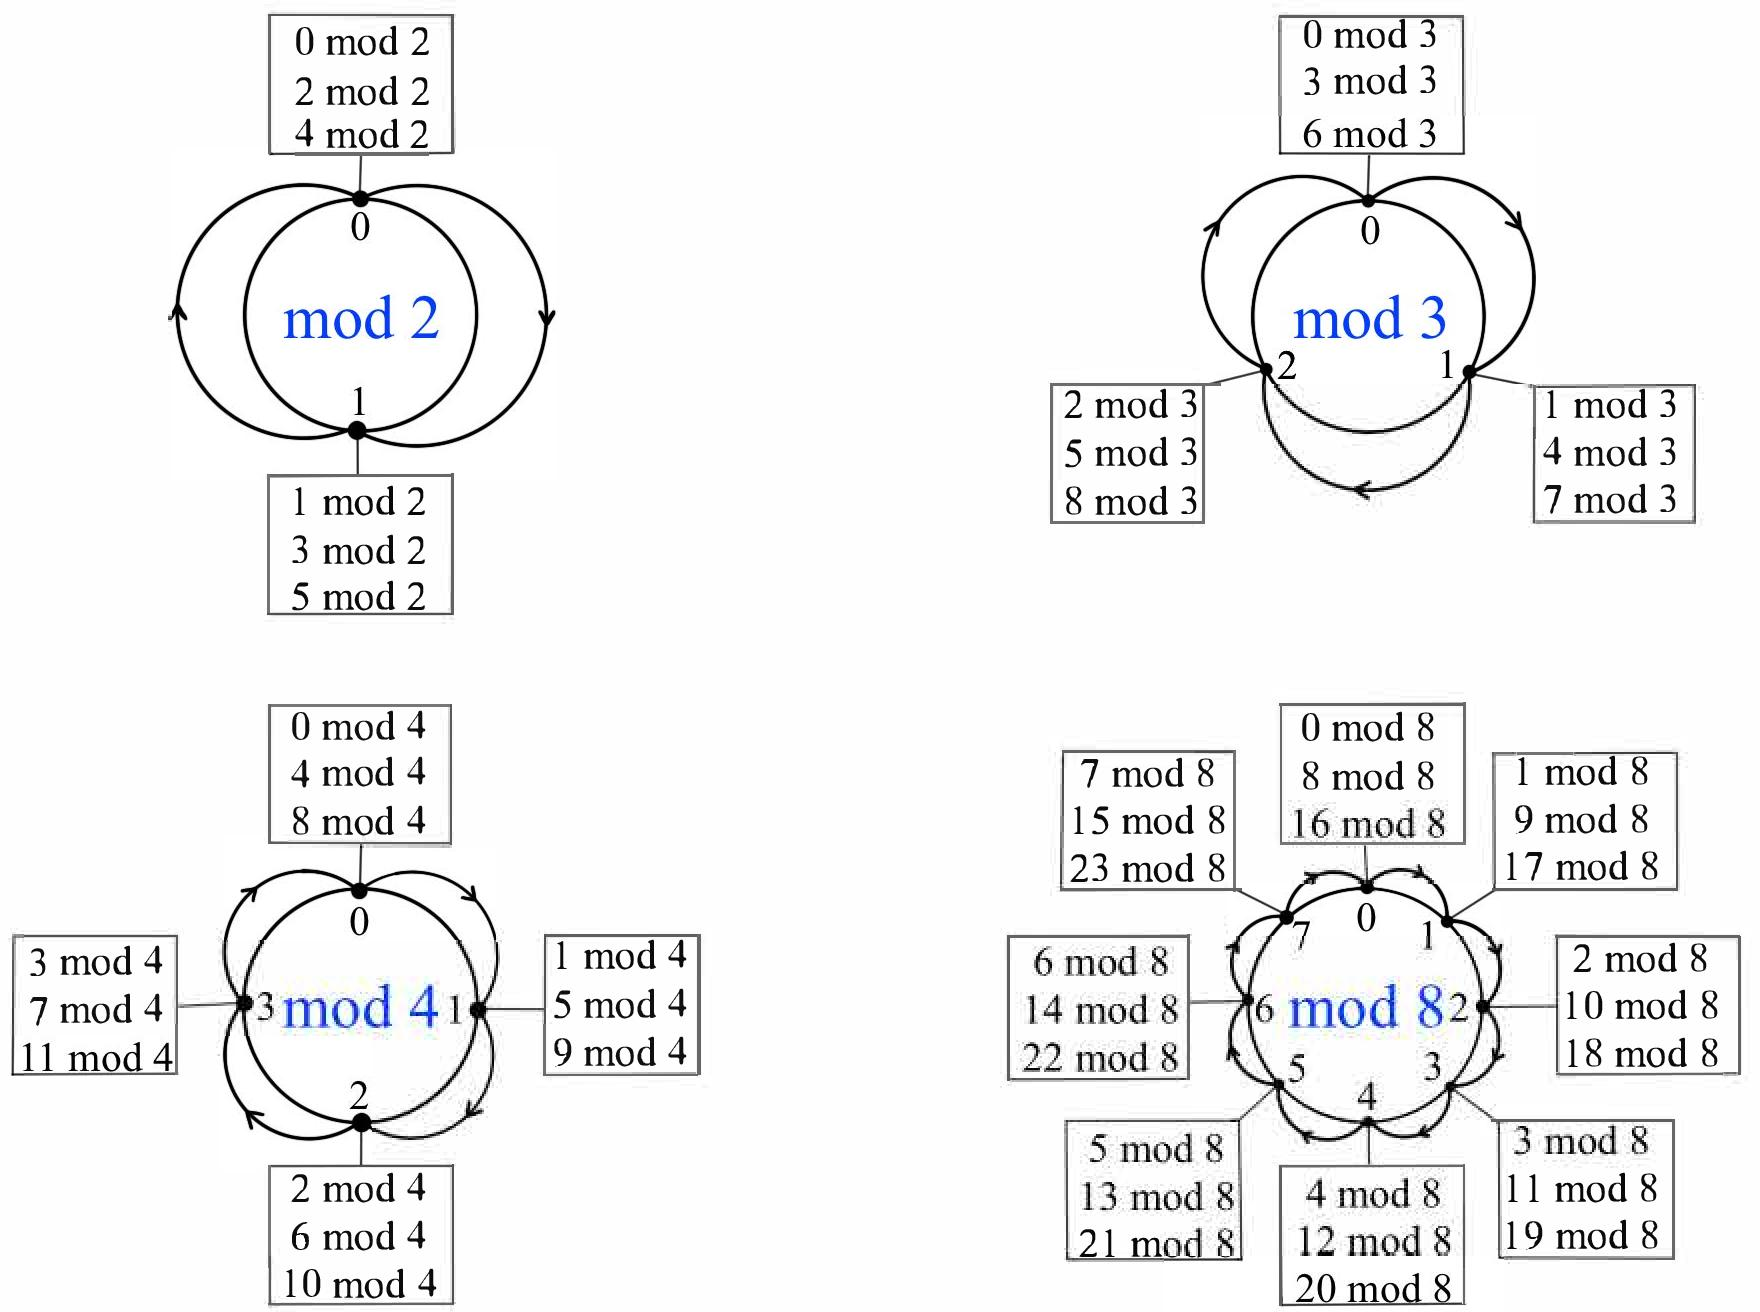
\includegraphics[scale=1]{Chapter1/images/necklace.png}} %Adym Warhurst

\begin{Exam}\label{exam:1.2modcalc} Let consider the following calculations: 
\begin{enumerate}
\item $6+11 \pmod 5$\\
\[6+11\equiv 17\equiv \fbox{$2$} \pmod 5\]
\item $7+13 \pmod 5$\\
\[7+13 \equiv 20\equiv \fbox{$0$} \pmod 5\]
\item\label{item:1.2inverse} $2(4) \pmod{7}$\\
\[2(4) \equiv 8\equiv 1 \pmod 7.\]
\item $2(5+6) \pmod{13}$\\
\[ 2(5+6) \equiv 2(11) \equiv 22 \equiv \fbox{$9$} \pmod{13}\]
\item $3(5)+8 \pmod{11}$\\
\[3(5)+8 \equiv 15+8 \equiv 4+8 \equiv 12 \equiv \fbox{$1$} \pmod{11}\qedhere\]
\end{enumerate}
\end{Exam}\vs

We can define \textbf{modular subtraction} $a-b \pmod n$ by adding the additive inverse of $b$ with respect to modular addition, that is, $a-b \equiv a+(-b)\pmod n$. Thus, modular subtraction is the inverse operation of modular addition. Returning to the pearl necklace analogy above, if $a+b\pmod n$ turns the necklace to the right (counter-clockwise) $b$ times from $a$, $a-b\pmod n$ turns the necklace to the left (clockwise) $b$ times from $a$. For example, starting at $2$ and counting backward on the necklace with $5$ pearls $4$ times gives the pearl $3$, that is, $2-4\equiv 3\pmod 5$. Likewise, $14-5 \equiv 9 \equiv 1\pmod 8$. %(Brittany Palmer)
Note that $-b \equiv n-b \pmod n$. Thus, the final result when computing modular subtraction should always be positive.\\ %Example by Zach Rogers

Similarly, we define  \textbf{modular division} $a/b \pmod n$ by multiplying by the multiplicative inverse of $b$ with respect to modular multiplication, that is, $a/b \equiv ab^{-1} \pmod n$. This multiplicative inverse will be an element of $\Z_n$ such that $bb^{-1} \equiv 1 \pmod n$, that is, their product will be one more than a multiple of $n$ as this implies the remainder is $1$ when divided by $n$ (see Example \ref{exam:1.2modcalc}.\ref{item:1.2inverse}). For example, \[4^{-1} = \dfrac{1}{4}\equiv 2 \pmod 7\] since $4(2) = 8 \equiv 1\pmod 7$. Thus, \[\dfrac{5}{4} \equiv 5(2) = 10 \equiv 3\pmod 7.\]  This multiplicative inverse does not always exists (see Exercise \ref{ex:1.2nosoln}).\\ %Example by Zach Rogers

 Alternatively, one can simplify a modular fraction without a multiplicative inverse by replacing the numerator with an integer equivalent to the original but actually divisible by the denominator in the usual sense. For example, \[\dfrac{17}{3} \equiv \dfrac{17+10}{3} \equiv \dfrac{27}{3} \equiv \dfrac{9(3)}{3} \equiv 9\pmod 5.\] The following theorem characterizes when this can be done.\\

\begin{Thm} The set $\Z_n$ is a field with respect to modular addition and modular multiplication if and only if $n$ is a prime number.
\end{Thm}\vs

\begin{Exam} Solve the linear equation $2x+1\equiv 6 \pmod{13}$. \\ 

Since $\Z_{13}$ is a field, we can solve this linear equation in the same fashion as the previous ones. Note
\[2x+1\equiv 6 \qRightarrow 2x \equiv 6-1 \equiv 5 \pmod {13} \qRightarrow x \equiv \dfrac{5}{2} \equiv 5(2)^{-1}.\] Next, we need to either identify the reciprocal of $2 \pmod{13}$\footnotemark[2] or replace $5$ with a congruent integer which is even, that is, $\dfrac{5}{2} \equiv \dfrac{5+13}{2} \equiv \dfrac{18}{2} \equiv 9\pmod{13}$. Therefore, the solution is 9. We can check this solution:
\[2(9) +1 \equiv 18 + 1 \equiv 19 \equiv 6 \pmod{13}.\qedhere\]
\end{Exam}\vs 

\begin{Exam} Solve the linear equation $3x+5\equiv 1 \pmod{7}$. \\ %Luke Shaner

We solve this equation similar to the previous example over the field $\Z_{7}$. 
\[3x+5\equiv 1 \qRightarrow 3x \equiv 1-5 \equiv -4 \equiv 3 \pmod {7} \qRightarrow x \equiv \dfrac{3}{3} \equiv 1.\]  We can check this solution:
\[3(1)+5 \equiv 3+5 \equiv 8 \equiv 1 \pmod{7}.\qedhere\]
\end{Exam}\vs
 
%%%%%%%%%%%%%%%%%%% Exercises %%%%%%%%%%%%%%%%%%%
\startExercises{fields}

\begin{enumerate}[!HW!, start=1]
\item Explain the difference between equality of \hyperref[note:integers]{integers} and \hyperref[def:modularcongruence]{congruence modulo $p$}. %Adam Maxwell
\end{enumerate}

\noindent For Exercises \ref{true:fieldsstart}-\ref{true:fieldsstop}, determine with the statement is true or false. If false, correct the statement so that it is true.
\begin{enumerate}[!HW!]
\item\label{true:fieldsstart} The remainder $a\pmod n$ is read ``$a$ modulo $n$'' and $a$ is called the modulus of \hyperref[note:mod]{$\Z_n$}. %Carson Blickenstaff
\item It is possible for two different integers to have the same residue modulo $n$. %Carson Blickenstaff
\item Modular division $a/b\pmod n$ is defined by multiplying by the inverse of $b$ with respect to modular addition. %Carson Blickenstaff
\item The set $\Z_n$ is a field with respect to modular addition and multiplication if and only if $n$ is a real number. %Carson Blickenstaff
\item\label{true:fieldsstop} If $0\le a< n$, then $a\pmod n=n$.\\ %Carson Blickenstaff
\end{enumerate}

\noindent For Exercises \ref{exer:modsimplifystart}-\ref{exer:modsimplifystop}, simplify the \hyperref[exam:1.2modcalc]{modular expression}. 
\begin{enumerate}[!HW!]
\begin{multicols}{4}
\item\label{exer:modsimplifystart} $-4\pmod{7}$ %Hamza Samha
\item $-21\pmod{5}$ %Hamza Samha
\item $-1076 \pmod{4}$ %Hamza Samha
\item $-686 \pmod{13}$ %Hamza Samha
\end{multicols}
\begin{multicols}{4}
\item $2237 \pmod{11}$ %Jaden Torgerson
\item $\dfrac{1}{2} \mod 3$ %Morganne Skelton
\item $\dfrac{1}{3} \mod 7$ %Morganne Skelton
\itemspade $34 + 61 \pmod{7}$
\end{multicols}
\begin{multicols}{3}
\itemspade $4(13) \pmod 5$
\item $5(15)\pmod 6$ %Yinglong Niu
\item $2(8-5) +4 \pmod 3$ %Yinglong Niu
\end{multicols}
\begin{multicols}{2}
\itemspade $2(6-3)+7 \pmod 2$
\itemspade $3[2+1-(6+3)] +6(7) \pmod{13}$
\end{multicols}
\begin{multicols}{3}
\itemspade $\dfrac{5(4)+3}{2(6)} \pmod{7}$
\item $\dfrac{3(5)+4}{2(7)} \pmod 9$ %Yinglong Niu
\item $\dfrac{6(7)+5}{2(4)} \pmod{13}$ %Heming Zu
\end{multicols}
\begin{multicols}{2}
\item $2[(3+4+2+5)+1+2(3)-3+2(-2)] \pmod 7$ %Mattie Zeigler
\item\label{exer:modsimplifystop} $\dfrac{4(9)+1-(6+12)}{1+3(6)} \pmod{13}$ %Mattie Zeigler
\end{multicols}
\item $\dfrac{-2(35-74)}{3} \pmod{19}$ %Sarah Walters
\end{enumerate}\vs

\noindent For Exercises \ref{exer:fieldequationRealstart}--\ref{exer:fieldequationRealstop}, solve the \hyperref[note:lineareqn]{linear equation}.  
\begin{enumerate}[!HW!]
\begin{multicols}{3}
\item\label{exer:fieldequationRealstart} $7x+10=3$ %Jaxton Maez
\itemspade $6x+7=2$
\itemspade $(2+i)x + (5-7i) = 3-4i$
\end{multicols}
\begin{multicols}{3}
\item $3x+7\equiv 5 \pmod 5$ %Kaylee Hall
\itemspade $x+1\equiv 0 \pmod 2$ 
\itemspade $2x+3\equiv 4 \pmod 5$ 
\end{multicols}
\begin{multicols}{3}
\itemspade $3x+2\equiv 1 \pmod 7$ 
\itemspade $5x+1\equiv 4 \pmod{11}$ 
\item $420x-7\equiv 98 \pmod{11}$  %Jaden Torgerson
\end{multicols}
\begin{multicols}{3}
\item $2x+5\equiv 0 \pmod 7$ %anon
\item $14x+12\equiv 124\pmod 6$ %Courtney Flanigan
\item $5x-25\equiv 71\pmod{14}$ %Courtney Flanigan
\end{multicols}
\begin{multicols}{3}
\item $2x-4\equiv 14\pmod 7$ %Courtney Flanigan
\item $3(2-4(x+1))\equiv 27\pmod 3$ %Courtney Flanigan
\item $-20-4x\equiv 40\pmod 4$ %Courtney Flanigan
\end{multicols}
\begin{multicols}{3}
\item $5x+22\equiv 15 \pmod 8$ %Grayson Walker
\item $6x+\frac{5}{2} \equiv 0 \pmod 7$ %Da Huo
\item\label{exer:fieldequationRealstop} $(3+10)x+2(7)+3\equiv 5(14) \pmod 7$ %anon
\end{multicols}
\end{enumerate}

\begin{enumerate}[!HW!]
\itemspade\label{ex:1.2nosoln} Show that the \hyperref[note:lineareqn]{linear equation} $2x+3\equiv 4 \pmod 6$ has no solution. 
\end{enumerate}

%%%%%%%%%%%%%%%%%%% Footnotes %%%%%%%%%%%%%%%%%%%
\mbox{}\vfill

\footnotetext[2]{By the way, the reciprocal of $2$ modulo $13$ is $7$ since $2(7) \equiv14\equiv 1 \pmod{13}$. Note that $x\equiv 5(2)^{-1} \equiv 5(7) \equiv 35 \equiv 9 \pmod{13}$.}
\pagebreak%1.2 Fields
\begin{center} 
\emph{``Your sacred space is where you can find yourself again and again.'' -- Joseph Campbell}
\end{center}

\section{Vector Spaces}\label{sec:vector}

Now that we have learned about fields and linear equations, the next important linear structure should discuss is that of \emph{linear combination}. In order to define this, we first need a notion of a vector. We say that a mathematical quantity is a \emph{vector} if we can add two vectors together to create a third vector and we can scale a vector by a scalar (hence the name). Vectors are distinct from scalars. While a scalar is a number, a vector is more complicated than just a number. To distinguish the extra complexity of vectors, vector quantities are denoted either in boldface font, such as $\bb u, \bb v$, or with an arrowhead above the symbol, such as $\vec u, \vec v$. The following definition makes precise this notion.\\

\begin{Def}\label{def:vectorspace} A \textbf{vector space} over a field $F$ is a nonempty set $V$ of elements, called \textbf{vectors}, on which are defined two operations, called \textbf{addition} $+ : V\times V \to V$ and \textbf{scalar multiplication} $\cdot : F\times V \to V$, such that for all $\bb u, \bb v, \bb w \in V$ and all scalars $c, d\in F$, the following eight axioms hold:
\setlength{\columnsep}{30pt}
\begin{multicols}{2}
\begin{enumerate}[!DEF!, start=1]
\item\label{item:vsaddassoc} \textbf{Additive Associativity}: $\bb u + \bb v = \bb v + \bb u$ 
\item\label{item:vsaddcomm} \textbf{Additive Commutativity}:\\ \mbox{}\hfill$(\bb u + \bb v) + \bb w = \bb u + (\bb v +  \bb w)$ 
\item\label{item:vsaddident} \textbf{Additive Identity}: There exists  a vector $\bb 0\in V$, such that $\bb u + \bb 0 = \bb 0 + \bb u = \bb u$ 
\item\label{item:vsaddinv} \textbf{Additive Inverse}: For each $\bb u$, there exists a vector $-\bb u\in V$, such that\\ \mbox{}\hfill$\bb u + (-\bb u) = (-\bb u) + \bb u = \bb 0$ \columnbreak
\item\label{item:vsleftdist} \textbf{Left Distributivity}: $c(\bb u + \bb v) = c\bb u + c\bb v$ 
\item\label{item:vsrightdist} \textbf{Right Distributivity}: $(c+d)\bb u = c\bb u + d\bb u$
\item\label{item:vsmultassoc} \textbf{Multiplicative Associativity}:\\ \mbox{}\hfill$c(d\bb u) = (cd)\bb u$ 
\item\label{item:vsmultiden} \textbf{Multiplicative Identity}: $1\bb u = \bb u$\\\\
\end{enumerate}
\end{multicols}
\end{Def}

\begin{Exam}\begin{multicols}{2}
In physics, a vector represents a mathematical quantity with both magnitude and direction, such as a force applied to an object. Vectors are thus represented as arrows pointing in the given direction and whose length represents the magnitude of the vector. Physical vectors are also free to move about in space, that is, this exact location does not matter so long as their length nor direction does not change. Therefore, the\columnbreak

\mbox{}
\begin{center}
\begin{tikzpicture}
\draw[-latex, ultra thick] (0,0) -- (1,1) node[midway, below right] {$\bb v$};
\draw[-latex, ultra thick, blue] (3,2) -- (4,3) node[midway, below right] {$\bb v$};
\draw[-latex, ultra thick, red] (-1,2) -- (0,3) node[midway, below right] {$\bb v$};
\end{tikzpicture}
\end{center}
\end{multicols}
\vspace{-10 pt} \noindent
 three arrows illustrated above represent that same vector $\bb v$. Hence, the arrow is determined by the relative displacement of the head of the arrow from its tails. These vectors can be added together by the so-called \emph{parallelogram rule}: begin by placing the tails of the two vectors $\bb u$ and $\bb v$ together, form a parallelogram whose parallel sides correspond to $\bb u$ with a copy of $\bb u$ and $\bb v$ with a copy of $\bb v$; the sum $\bb u + \bb v$ is the unique vector which is the diagonal of the parallelogram whose tail agrees with the tail of $\bb u$ and $\bb v$, as displayed:

\begin{multicols}{3}
\begin{center}
\begin{tikzpicture}
\draw[dashed, ultra thick, gray] (1,2) -- (4,3);
\draw[dashed, ultra thick, gray] (3,1) -- (4,3);
\draw[-latex, ultra thick] (0,0) -- (3,1) node[midway, below right] {$\bb v$};
\draw[-latex, ultra thick] (0,0) -- (1,2) node[midway, above left] {$\bb u$};
\draw[-latex, ultra thick, red] (0,0) -- (4,3) node[midway, above, yshift = -5] {\rotatebox{35}{$\bb u + \bb v$}};
%\path(2,-1) node[below] {The Parallelogram Rule};
\end{tikzpicture}
\vfill \textbf{The Parallelogram Rule}
\end{center}

\begin{center}
\begin{tikzpicture}
\draw[dashed, ultra thick, gray] (1,2) -- (4,3) node[above left, midway] {$\bb v$};
\draw[dashed, ultra thick, gray] (0,0) -- (1,2) node[above left, midway] {$\bb u$};
\draw[-latex, ultra thick] (0,0) -- (3,1) node[midway, below right] {$\bb v$};
\draw[-latex, ultra thick] (3,1) -- (4,3) node[midway, right] {$\bb u$};
\draw[-latex, ultra thick, red] (0,0) -- (4,3) node[midway, above, yshift = -5] {\rotatebox{35}{$\bb u + \bb v$}};
\end{tikzpicture}
\vfill $\bb u + \bb v = \bb v + \bb u$
\end{center}

\begin{center}
\begin{tikzpicture}
\draw[, ultra thick, dashed, gray] (0,0) -- (-1,2.25) node[midway, below, sloped] {$\bb u+\bb v$};
\draw[, ultra thick, dashed, gray] (2,1) -- (2,4) node[midway, below, sloped] {$\bb v+\bb w$};
\draw[-latex, ultra thick] (0,0) -- (2,1) node[midway, below right] {$\bb u$};
\draw[-latex, ultra thick] (2,1) -- (-1,2.25) node[midway, below left] {$\bb v$};
\draw[-latex, ultra thick] (-1,2.25) -- (2,4) node[midway, above left] {$\bb w$};
\draw[-latex, ultra thick, red] (0,0) -- (2,4) node[pos=0.65, sloped, above] {$\bb u + \bb v + \bb w$};
\end{tikzpicture}
\end{center}
\vfill $(\bb u + \bb v) + \bb w = \bb u + (\bb v + \bb w)$
\end{multicols}
The second diagram shows why arrow addition is commutative, as the two paths from the tail of $\bb u+\bb v$ to head produce the same vector. In particular, the black, solid path comprises $\bb v+\bb u$ while the gray, dashed path comprises $\bb u+\bb v$, and both paths have the same starting and ending points. The third diagram likewise demonstrates how three or more vectors are added together and why arrow addition is associative, as the path following $(\bb u + \bb v)$ then $\bb w$ produces the same vector as the path following $\bb u$ then $(\bb v+\bb w$).

The zero vector $\bb 0$ would be simply a point in space, that is, the vector with no magnitude nor direction. Notice that adjoining a point to the head or tail will neither lengthen the arrow nor turn it. Thus, $\bb v+\bb 0 =\bb v$. Additionally, given a vector $\bb v$, $-\bb v$ is defined as the arrow with the same length but pointing in the opposite direction. It holds that $\bb v + (-\bb v) = (-\bb v) + \bb v = \bb 0$.
\begin{center}
\begin{tikzpicture}
\draw[->, ultra thick] (0,0) -- (1,1) node[midway, below right] {$\bb v$};
\draw[->, ultra thick, blue] (3,1) -- (2,0) node[midway, below right] {$-\bb v$};
\end{tikzpicture}
\end{center}

\noindent We define scalar multiplication of arrows by multiplying the length of the arrow by the scalar (and switching directions if the scalar is negative). Clearly, $1\bb v=\bb v$, since the length of the arrow is unchanged, and $c(d\bb u) = (cd)\bb u$, since stretching a vector by a factor of $d$ then stretching by a factor of $c$ as the net affect of stretching the arrow by a factor of $cd$. It is left as an exercise of the reader to prove that two distributive laws. Therefore, the set of arrow in space forms a vector space under these operations.
\end{Exam}\vs

\begin{Exam}
Another type of vector is an array of numbers. Let $F$ be a field. Then a \textbf{column vector} is an array of $n$ scalars from $F$ such that the array is oriented vertically, e.g. $\bb v = \vr{1\\2\\3}$. A \textbf{row vector} likewise is an array of $n$ scalars such that the array is oriented horizontally, e.g.  $\bb v =(1, 2, 3)$. Our notation of a row vector agrees with the commonly used  notation  for coordinates of points in Cartesian geometry. As such, we naturally identify these arrays of scalars with points in space. The difference between row vectors and column vectors is purely notational, and we will use the two notations interchangeably.\footnotemark[2]  The order of the scalars in the array does matter, e.g. $(1, 2, 3) \neq (2,3, 1)$.\\

Let $F^n$ denote the set of all column vectors with $n$ entries coming from the field $F$, for example, for example, \[\mtx{c}{\pi\\ 0\\ -\sqrt{17}} \in \R^3,\quad \vr{1-2i \\  \frac{1}{2}-\frac{5}{2}i}\in \C^2,\quad \text{ or }\quad \vr{1\\2\\0\\2\\1}\in \Z_3^5.\footnotemark[8]\]

Addition of column vectors is component-wise, that is, scalars in the corresponding positions are added together:
\begin{equation} \bb u+ \bb v = \mtx{c}{u_1\\u_2\\\vdots\\u_n} + \mtx{c}{v_1\\v_2\\\vdots\\v_n} = \mtx{c}{u_1+v_1\\u_2+v_2\\\vdots\\u_n+v_n}. \end{equation}  For scalar multiplication, every component is multiplied by the scalar, that is:
\begin{equation} c\bb x = c\mtx{c}{x_1\\x_2\\\vdots\\x_n}= \mtx{c}{cx_1\\cx_2\\\vdots\\cx_n}. \end{equation}   Here the zero vector $\bb 0$ is the array of all zeros and $-\bb v=(-1)\bb v$. We show that this definition of vector addition satisfies the additive associativity axiom:
\begin{multline*}\bb u+(\bb v+\bb w) = \mtx{c}{u_1\\u_2\\\vdots\\u_n} + \left(\mtx{c}{v_1\\v_2\\\vdots\\v_n} + \mtx{c}{w_1\\w_2\\\vdots\\w_n}\right) = \mtx{c}{u_1\\u_2\\\vdots\\u_n} + \mtx{c}{v_1+w_1\\v_2+w_2\\\vdots\\v_n+w_n} = \mtx{c}{u_1+(v_1+w_1)\\u_2+(v_2+w_2)\\\vdots\\u_n+(v_n+w_n)}\\ \overset{(*)}{=} \mtx{c}{(u_1+v_1)+w_1\\(u_2+v_2)+w_2\\\vdots\\(u_n+v_n)+w_n)} = \mtx{c}{u_1+v_1\\u_2+v_2\\\vdots\\u_n+v_n} + \mtx{c}{w_1\\w_2\\\vdots\\w_n} = \left(\mtx{c}{u_1\\u_2\\\vdots\\u_n} + \mtx{c}{v_1\\v_2\\\vdots\\v_n}\right) + \mtx{c}{w_1\\w_2\\\vdots\\w_n} = (\bb u + \bb v) + \bb w,
\end{multline*} where the marked equality $(*)$ follows from the additive associtivity of the field $F$. The remaining axioms of a vector space are left as an exercise to the reader. Therefore, $F^n$ is a vector space, the one we will place the most focus on in this text.
\end{Exam}\vs

\begin{Exam} Let $\bb u = \vr{ 6\\-2\\ 2}, \bb v = \vr{ -3\\0\\ 5} \in \R^3$. Then 
\[\bb u + \bb v = \vr{ 6\\-2\\ 2} + \vr{ -3\\0\\ 5} = \vr{ 6-3\\ -2+0\\ 2+5} = \vr{ 3\\ -2\\ 7}.\]
 If $\bb v = \vr{-1\\ 3\\2}\in \R^3$, then 
\[3\bb v = 3\vr{-1\\ 3\\2} = \vr{ -3\\ 9\\6}. \qedhere\]
\end{Exam}\vs

\begin{Def}\label{def:linearcombo} Given vectors $\bb v_1, \bb v_2, \ldots, \bb v_n\in F^m$ and scalars $c_1, c_2, \ldots, c_n\in F$, the vector $\bb x$ given as 
\[\bb x = c_1\bb v_1 + c_2\bb v_2 + \ldots + c_n\bb v_n\] is called a \textbf{linear combination} of $\bb v_1, \bb v_2, \ldots, \bb v_n$ with \textbf{coefficients} $c_1, c_2, \ldots, c_n$. \\
\end{Def}\vs

A linear combination is a way of combining vectors using addition and scalar multiplication. These vectors operations, of course, depend entirely on the field of scalars.\\

\begin{Exam} Let us simplify the following linear combinations over the vector spaces $\C^2$ and $\Z_3^3$, respectively.
\begin{enumerate}
\item $2\mtx{c}{3\\ i} + i\mtx{c}{2+i\\ 3+5i} = \mtx{c}{6\\2i} + \mtx{c}{-1+2i\\ -5+3i} = \mtx{c}{6+(-1+2i)\\ 2i + (-5+3i)} = \mtx{c}{5+2i\\-5+5i}$.\\

\item $\vr{0\\1\\2} + 2\vr{1\\1\\1} + 2\vr{1\\0\\2} \equiv \vr{0\\1\\2} + \vr{2\\2\\2} + \vr{2\\0\\1} \equiv \mtx{c}{0+2+2\\ 1+2+0\\2+2+1} \equiv \mtx{c}{4\\3\\5} \equiv \mtx{c}{1\\0\\2} \pmod 3. \hfill\qedhere$
\end{enumerate}
\end{Exam}\vs

Vectors can also be many other things, like matrices,  functions, sequences of numbers. Even linear equations can be vectors. \\

\begin{Exam}\label{exam:vectorspaceproof} Let $V$ be the set of linear equations with $n$ variables, say $x_1, x_2,\ldots, x_n$ with coefficients coming from the field $F$.  For example, 
\[c_1x_1+\ldots + c_nx_n = b_1\] is an element of $V$ for $c_1,\ldots, c_n, b_1\in F$. Likewise, if \[d_1x_1+\ldots + d_nx_n=b_2\] is another linear equation in $V$, then 
\[\begin{alignedat}{100}
&& (c_1x_1\ &+\ & \ldots\ & +\ & c_nx_n\ & =\ & b_1) \\
+\ && (d_1x_1\ &+\ &\ldots\ & +\ & d_nx_n\ &=\ &b_2)\\ \hline
&&(c_1+d_1)x_1\ &+\ & \ldots\ & +\ & (c_n+d_n)x_n\ & =\ & (b_1+b_2)
\end{alignedat}\] Note that $c_i+d_i, b_1+b_2\in F$ for all $i$. Thus, the sum of equations is a member of $V$, that is, it is a vector too. Similarly, if $a\in F$, then $c_1x_1+\ldots + c_nx_n = b_1$ scaled by $a$ is the linear equation 
 \[(ac_1)x_1+\ldots + (ac_n)x_n = (ab_1).\] As $ac_i, ab_1\in F$ for all $i$, this equation is likewise a vector. Therefore, $V$ is a vector space. Let $E_1, E_2, \ldots, E_m \in V$ be a list of linear equations with common solution $\bb x \in F^n$. Then $\bb x$ is a solution to any linear combination $a_1E_1 + a_2E_2 +\ldots + a_mE_m$. 
\end{Exam}\vs

\begin{Thm}\label{thm:vectorprop} The following properties hold for any $F$-vector space $V$. Let $\bb u \in V$ and $c\in F$.
\begin{enumerate}[!THM!, start=1]
\begin{multicols}{2}
\item\label{item:vectorpropuniquezero} The zero vector $\bb 0$ in $V$ is unique.\\
\item\label{item:vectorpropuniqueinverse} The additive inverse of $\bb u$ is unique.\\
\end{multicols}
\begin{multicols}{3}
\item\label{item:vectorpropzeroscalar} $0\bb u = \bb 0$.\\
\item\label{thm:vectorpropzerovector} $c\bb 0 = \bb 0$.\columnbreak
\item\label{thm:vectorpropnegscalar} $-\bb u = (-1)\bb u$.
\end{multicols}
\end{enumerate}
\end{Thm}
\begin{proof}
\begin{enumerate}[!DEF!,start=1]
\item Suppose there is a vector $\bb\theta \in V$ such that $\bb\theta + \bb v = \bb v + \bb\theta = \bb v$ for all $\bb v\in V$. Then 
\[\bb 0 = \bb 0 + \bb \theta = \bb \theta.\] Therefore, $\bb 0$ is the unique vector with this property.\\

\item Like the last property, suppose that $\bb u' \in V$ has the property that $\bb u + \bb u' = \bb u' + \bb u = \bb 0$. Then
\[\bb u' = \bb u' + \bb 0 = \bb u' + (\bb u + -\bb u) = (\bb u' + \bb u) + -\bb u = \bb 0 + -\bb u = -\bb u.\] Therefore, $-\bb u$ is the unique vector with this property.\\

\item First, \[0\bb u = (0+0)\bb u = 0\bb u + 0\bb u.\] Adding $-0\bb u$ to both sides of the equation gives $\bb 0 = 0\bb u$.\\

The remaining parts are left as exercises to the reader.\hfill$\qedhere$
%\item Now, 
%\[\bb 0 = 0\bb 0 = (c0)\bb 0  = c(0\bb 0) = c\bb0.\]
%
%\item Finally, 
%\[\bb u + (-1)\bb u = 1\bb u + (-1)\bb u = (1-1)\bb u = 0\bb u = \bb 0.\] Therefore, $(-1)\bb u = -\bb u$. \hfill$\qedhere$
\end{enumerate}
\end{proof}

%%%%%%%%%%%%%%%%%%% Exercises %%%%%%%%%%%%%%%%%%%
\startExercises{vector}

\noindent For Exercises \ref{true:vsstart}-\ref{true:vsstop}, determine with the statement is true or false. If false, correct the statement so that it is true.
\begin{enumerate}[!HW!, start=1]
\item\label{true:vsstart}\label{true:vsstop} For any \hyperref[def:vectorspace]{vector space} $V$, $\emptyset\in V$. %Da Huo
\end{enumerate}

\noindent For Exercises \ref{exer:linearcomborealstart}-\ref{exer:linearcomborealstop}, simplify the \hyperref[def:linearcombo]{linear combination}. 
\begin{enumerate}[!HW!]
\begin{multicols}{2}
\item\label{exer:linearcomborealstart} $5\vr{1\\2\\4}+3\vr{0\\2\\1}+4\vr{1\\1\\1}$ %Cameron Dix
\itemspade $3\vr{-1\\0\\1} + 2\vr{0\\0\\1}-2\vr{3\\4\\0}$
\end{multicols}
\begin{multicols}{2}
\item $\vr{3\\2\\1} + \mtx{c}{5\\8\\10} + \vr{0\\0\\5}$ %Sherie Ayag
\item $-1\vr{3\\0\\1}+\vr{1\\2\\4} + 3\vr{2\\4\\1}$ %Jacob Newey
\end{multicols}
\begin{multicols}{2}
\item $7\vr{3\\0\\2}+2\vr{8\\-3\\5}-3\vr{-2\\-2\\0}$ %Grayson Walker
\item $8\vr{1\\4\\3} +2\vr{5\\0\\4} -4\vr{1\\0\\1}$ %Yinglong Niu
\end{multicols}
\begin{multicols}{2}
\item $(2+5i)\vr{3\\4} - (3-2i)\mtx{c}{7+i\\6+2i}$ %Heming Zu
\itemspade $(3+2i)\vr{1\\2} -(1-2i)\mtx{c}{3+4i \\ 1+i}$
\end{multicols}
\begin{multicols}{2}
\item $(2+i)\mtx{c}{1+i\\i} + \mtx{c}{2i\\1+2i}$ %Cameron Dix
\item $(2+4i)\vr{2\\3} - (3-2i)\mtx{c}{1+2i\\2-i}$ %Jaimie Goldberg 
\end{multicols}
\begin{multicols}{2}
\item $(1+i)\mtx{c}{1-i\\2+i}-(1-i)\mtx{c}{3+i\\4-i}$ %Yinglong Niu
\item $(1-i)\mtx{r}{1\\2\\-1} + \vr{2\\3\\5} -(2+3i)\vr{1\\4\\2}$ %Jacob Newey
\end{multicols}
\begin{multicols}{2}
\item $(4+5i)\vr{3\\5\\2} +(3-2i)\vr{1+3i\\2-3i\\2+5i}$ %Kyle Wood
\item $2\vr{2\\1} - \vr{1\\0} +2\vr{1\\1} \pmod3$ %Jacob Newey
\end{multicols}
\begin{multicols}{2}
\item $-10\vr{3\\2}+\vr{5\\6} \pmod7$ %Cameron Dix
\itemspade $\vr{1\\0\\1} + \vr{1\\1\\0} + \vr{1\\1\\1} \pmod 2$
\end{multicols}
\begin{multicols}{2}
\item $6\vr{1\\3\\4} + 2\vr{1\\1\\5} + \vr{1\\1\\1} \pmod 3$ %Kaylee Hall
\item $\vr{3\\4\\3}+\vr{4\\1\\1}+\vr{0\\1\\1} \pmod5$ %Cameron Dix
\end{multicols} \pagebreak
\begin{multicols}{2}
\item $2\vr{1\\2\\3}+3\vr{3\\2\\1}+4\vr{0\\1\\0}\pmod5$ %anon
\itemspade $4\vr{1\\0\\0\\2} + 2\vr{2\\3\\1\\0} + \vr{1\\2\\3\\4}\pmod5$
\end{multicols}
\begin{multicols}{2}
\item $3\vr{-1\\2\\-3\\0}-2\vr{1\\2\\2\\1}+\vr{2\\3\\0\\1}\pmod5$ %Jacob Newey

\item \label{exer:linearcomborealstop} $\vr{4\\2\\3\\1} + 2\vr{0\\1\\4\\3} + 3\vr{1\\1\\2\\3}\pmod5$\ %Hailey Checketts
\end{multicols}
\end{enumerate}

\begin{enumerate}[!HW!]
\itemspade Prove parts \ref{thm:vectorpropzerovector} and \ref{thm:vectorpropnegscalar} of \thmref{thm:vectorprop}.
\end{enumerate}
\begin{enumerate}[!HW!, label=$\spadesuit$ \arabic*., ref=\arabic*]
\item\label{exer:polynomialspace} Let $\P_n =\{a_0 + a_1x + a_2x^2 + \ldots + a_nx^n \mid a_0, a_1, a_2,\ldots, a_n\in F\}$ be the set of polynomials of degree at most $n$ and coefficients from a \hyperref[def:field]{field} $F$. Show that $\P_n$ is a \hyperref[def:vectorspace]{vector space}, hence we may view polynomials as vector quantities. (More specifically, show that the sum of two polynomials is again a polynomial and the scalar multiple of a polynomial is likewise a polynomial, similar to the method introduced in Example \ref{exam:vectorspaceproof}).
\end{enumerate}

\noindent Note that the way we defined vector addition and scalar multiplication over \hyperref[note:Fn]{$F^n$} is essentially the only way to do it to guarantee the \hyperref[def:vectorspace]{vector space axioms}. For Exercises \ref{exer:vsNewScalarsstart}-\ref{exer:vsNewScalarsstop}, we will redefine scalar multiplication over $F^3$ (and keep vector addition the same). Find a counterexample for why this alternative definition of scalar multiplication fails at least one \hyperref[def:vectorspace]{vector space axiom} or property and hence does not produce a genuine vector space. Answers may vary.
\begin{enumerate}[!HW!, label=$\spadesuit$ \arabic*., ref=\arabic*]
\begin{multicols}{2}
\item\label{exer:vsNewScalarsstart} Redefine scaling: $c\vr{x_1\\x_2\\x_3} = \vr{x_1\\x_2\\x_3}$
\item Redefine scaling: $c\vr{x_1\\x_2\\x_3} = \mtx{c}{cx_1\\x_2\\x_3}$
\end{multicols}
\begin{multicols}{2}
\item Redefine scaling: $c\vr{x_1\\x_2\\x_3} = \vr{-cx_1\\-cx_2\\-cx_3}$
\item\label{exer:vsNewScalarsstop} Redefine scaling: $c\vr{x_1\\x_2\\x_3} = \mtx{c}{0\\cx_2\\cx_3}$
\end{multicols}
\end{enumerate}

\pagebreak
%%%%%%%%%%%%%%%%%%% Footnotes %%%%%%%%%%%%%%%%%%%
\mbox{}\vfill

\footnotetext[2]{From a vector perspective, the notion of a column vector $\vr{1\\2\\3}$, a row vector $[1\ 2\ 3]$, and a geometric point $(1,2,3)$ are all the same. Why have different notations then? In other contexts, it is helpful to distinguish between them. In calculus or physics, a distinction between points and vectors (aka arrows) is sometimes desired (although often unnecessary). Thus, points have their usual notation and arrows are given a different notation, which may include the column or row vector notation we have already introduced or some other notation that we will not use here, e.g. $\langle 1, 2, 3\rangle$. As arrows can be moved anywhere in space without changing their value, the vectors are often placed in \emph{standard position}, meaning its tail is on the origin. Then the head of the arrow is a unique point in space which characterizes this arrow. This standard representation of the vector, sometimes called its \emph{algebraic form}, is very desirable as the algebraic computations are far simpler their their geometric counterparts. For this reason, we see not strong reason to distinguish between arrows in space and the coordinates that they are pointing at. The only perspective that we will distinguish between a column vector and a row vector herein is when we consider them matrices, such as in \chapref{3rd}. This may be imperative for matrix operations, such as multiplication. Under the matrix perspective, a column vector is just an $n\times 1$ matrix, and a row vector is just a $1\times n$ matrix.}

%Andrew Biskey
\footnotetext[8]{The combined notations of the set $\Z_p$, which is a field whose subscript defines the modulus, and the vector space $F^n$, whose superscripts defines the number of entries in each vector, conveys information about the vector space $\Z_p^n$.  For example, $\Z_3^5$ denotes the vector space whose vectors comprise of five elements in the array that are integers congruent modulo 3, e.g, $\vr{1\\2\\0\\2\\1}$. Note that no integer in $\Z_3^n$ ever needs to be greater that $2$ or smaller than $0$, as all those integers are reducible modulo $3$. Hence, $\Z_3^5$ contains exactly $3^5=243$ distinct vectors. In general, the vector space $\Z_p^n$ will contain exactly $p^n$ many vectors.}
\pagebreak%1.3 Vector Spaces
\begin{center} 
\emph{``Don't spend time beating on a wall, hoping to transform it into a door.'' -- Coco Chanel}
\end{center}

\section{Linear Transformations}\label{sec:trans}

The next important linear structure we have seen before (primarily in calculus) is the notion of a \emph{linear operator} or a \textbf{linear transformation}. This is a function on vectors which preserve linear combinations.\\

\begin{Def}\label{def:linear} Let $X$ and $Y$ be vector space over a field $F$. A function $T : X \to Y$ is a \textbf{linear transformation} if:
\begin{enumerate}[!DEF!, start=1]
\item $T(\bb u + \bb v) = T(\bb u) + T(\bb v)$, for all vectors $\bb u, \bb v \in X$;
\item $T(c\bb u) = cT(\bb u)$, for all vectors $\forall \bb u\in X$ and scalars $c\in F$.
\end{enumerate}
Recall that $X$ and $Y$ are called the \textbf{domain} and \textbf{codomain} of $T$, respectively. For any $\bb x\in X$, we call $T(\bb x)$ the \textbf{image} of $T\bb x$, and we call $\im(T) = \{T(\bb x) \mid \bb x\in X\}$ (the set of images) the \textbf{image} (or \textbf{range}) of $T$. The \textbf{kernel} of a linear transformation $T$ is the set of vectors which map to the zero vector, that is, $\ker T = \{\bb x\mid T(\bb x) = \bb 0\}$, denoted $\ker(T)$.\\
\end{Def}

\begin{Exam} In calculus, there are many linear operators. For example, the derivative is a linear transformation since
\[\ddx[f(x)+g(x)] = \ddx[f(x)]+\ddx[g(x)]\qquad\text{and}\qquad \ddx[cf(x)] = c\ddx[f(x)].\] Note that $\ker \left(\ddx\right)$ is the set of constant functions. Likewise, limits are linear operators:
\[\lim_{x\to a}[f(x) + g(x)] = \lim_{x\to a}[f(x)] + \lim_{x\to a}[g(x)]\qquad\text{and}\qquad \lim_{x\to a}[cf(x)] = c\lim_{x\to a}[f(x)].\]
Likewise, antiderivatives, definite integrals, indefinite integrals, and series are all linear operators on functions. Linear algebra was everywhere in calculus, we just didn't know it!
\end{Exam}\vs

\begin{Prop} Let $T : X\to Y$ be a linear transformation. Let $\bb x_1, \ldots, \bb x_n\in X$ and $c_1,\ldots, c_n\in F$. Then 
\[T(c_1\bb x_1 + \ldots + c_n\bb x_n) = c_1T(\bb x_1)+\ldots + c_nT(\bb x_n).\] The converse also is true, that is, $T$ is a linear transformation if it preserves linear combinations. In particular, $T(\bb 0) = \bb 0$.
\end{Prop}\vs

\begin{Exam}\label{exam:lintrans} Consider the function $T : \R^3 \to \R^2$ given by the rule $T(x_1, x_2, x_3) = (x_1+2x_2, x_3-3x_2)$, or in vector notation as:
\[T\vr{x_1\\x_2\\x_3} =  \vr{x_1+2x_2\\ x_3-3x_2}.\] This is a function which takes a vector in 3-space, such as $(1,2,3)$, and maps it onto a vector in 2-space, namely $T(1,2,3)=(1+2(2), 3-3(2)) = (5,-3)$. But more than just a function that sends 3D vectors onto 2D vectors, this function \emph{preserves} the structure of the vector space $\R^3$ as it maps onto $\R^2$. This function is a linear transformation since 
\[T\left(a\vr{x_1\\x_2\\x_3} + b\vr{y_1\\y_2\\y_3}\right) = T\vr{ax_1+by_1\\ax_2+by_2\\ax_3+by_3} = \vr{(ax_1+by_1) +2(ax_2+by_2) \\ (ax_3+by_3)-3(ax_2+by_2)}\]
\[ a\vr{x_1+2x_2 \\ x_3-3x_2} + b\vr{y_1+2y_2\\y_3-3y_2} = aT\vr{x_1\\x_2\\x_3} + bT\vr{y_1\\y_2\\y_3}.\] 

We next compute the kernel of $T$. Suppose $T(\bb x) = \bb 0$. This implies that $\vr{x_1+2x_2\\ x_3-3x_2} = \vr{0\\0}$. Comparing components, we find two linear equations $x_1+2x_2=0$ and $x_3-3x_2=0$. Together, this forms a homogeneous system of linear equations. 
\[\begin{linear} x_1\ & +\ & 2x_2\ &&&=\ & 0\\
&-\ &3x_2\ & +\ & x_3\ &=\ & 0.\end{linear}\] If we attempt to solve this system, we could use the method of substitution. Note we can solve for $x_1$ in the first equation, which gives $x_1 = -2x_2$. Likewise, we can solve $x_3$ in the second equation and find $x_3=3x_2$. What we see now is that $x_1$ and $x_3$ are determined by our choice of $x_2$ and there appears to be NO restriction on our choice of $x_2$, that is, we may choose it freely.  For example, if $x_2=1$, it would mean that $x_1=-2$ and $x_3=3$, that is, $x_1$ and $x_3$ are dependent on $x_2$. Note that 
\[T\vr{-2\\1\\3} = \mtx{c}{(-2)+2(1)\\(3)-3(1)} = \mtx{c}{-2+2\\3-3} = \vr{0\\0} = \bb 0.\] Thus, this vector is in the kernel. In fact, the solution set to this system is exactly the kernel of $T$. If we let $x_2=t$, some free parameter $t$, then we see that \[\ker T = \left\{\mtx{c}{-2t\\ t \\ 3t}\ \middle|\ t\in \R\right\} = \left\{t\mtx{c}{-2\\ 1 \\ 3}\ \middle|\ t\in \R\right\} =  \Span\left\{\mtx{c}{2\\ -1 \\ -3}\right\}.\]

Is the vector $\bb b = \vr{1\\2}$ in the image of $T$? If so, there would be a vector $\bb x = \vr{x_1\\x_2\\x_3}$ such that $T(\bb x) = \bb b$. But this implies that $\vr{x_1+2x_2\\ x_3-3x_2} = \vr{1\\2}$. Again, this vector equation implies two linear equations, namely, $x_1+2x_2=1$ and $-3x_2+x_3=2$, which as a system of equations is
\[\begin{linear} x_1\ & +\ & 2x_2\ &&&=\ & 1\\
&-\ &3x_2\ & +\ & x_3\ &=\ & 2.\end{linear}\] Again by substitution, we see $x_1 = 1-2x_2$ and $x_3=2+3x_2$. Thus, if $x_2=0$, we get that 
\[T\left(\vr{1\\0\\2}\right) = \vr{1+2(0) \\ 2 - 3(0)} = \vr{1\\2}.\] Therefore, yes, $\bb b \in \im T$. Of course, many other choices of $\bb x$ were possible such that $T(\bb x) = \bb b$.
\end{Exam}\vs

Notice that the components of $T(\bb x)$ in the previous example are linear combinations of the components of the input vectors, that is, each slot in $T(\bb x)$ is a linear combination of the variables $x_1, x_2, \ldots$  It can be shown that a function $T : F^n \to F^m$ is a linear transformation if and only if the components of $T(\bb x)$ are linear combinations of the components of $\bb x$. Another takeaway from the previous example is that computing the kernel or image of a linear transformation resulted in solving a system of linear equations. This is no coincidence and we will discuss solving systems of linear equations more in the next sections. \\

%Christpher Houston
\begin{Exam} Consider the function $T : \hyperref[exer:polynomial space]{\mathcal{P}_2} \to \R^2$ given by the rule $T(ax^2+bx+c)=\mtx{c}{5a+2c\\-a+c}$.  Let $f(x) = a_1x^2+b_1x+c_1, g(x)=a_2x^2+b_2x+c_2\in \mathcal{P}_2$ and $r\in \R$. Then
\begin{multline*}T(f(x) + g(x)) = T((a_1x^2+b_1x+c_1) + (a_2x^2+b_2x+c_2)) = T((a_1+a_2)x^2+(b_1+b_2)x+(c_1+c_2))\\ = \mtx{c}{5(a_1+a_2) + 2(c_1+c_2)\\ -(a_1+a_2)+(c_1+c_2)} = \mtx{c}{(5a_1+2c_1)+(5a_2+2c_2)\\(-a_1+c_1) + (-a_2+c_2)} = \mtx{c}{5a_1+2c_1\\-a_1+c_1} + \mtx{c}{5a_2+2c_2\\-a_2+c_2}\\ = T(a_1x^2+b_1x+c_1) + T(a_2x^2+b_2x+c_2) = T(f(x)) + T(g(x))\end{multline*}
and
\begin{multline*}T(rf(x)) = T(r(a_1x^2+b_1x+c_1)) = T((ra_1)x^2+(rb_1)x+(rc_1)) \\ =\mtx{c}{5(ra_1)+2(rc_1)\\ -(ra_1)+(rc_1)} = \mtx{c}{r(5a_1+2c_1)\\ r(-a_1+c_1)} = r\mtx{c}{5a_1+2c_1\\ -a_1+c_1} =\\ rT(a_1x^2+b_1x+c_1)=rT(f(x)).\end{multline*} Therefore we see that $T$ is a linear transformation between the vector spaces $\mathcal{P}_2$ and $\R^2$. \\

To find the kernel of $T$, we must solve the vector equation $\mtx{c}{5a+2c\\-a+c} = \vr{0\\0}$, which corresponds to the linear system $\begin{linear}
5a\ &+\ &2c\ &=\ &0\\ -a\ &+\ &c\ &=\ &0&.
\end{linear}$ We solve this system by elimination. Scale the second equation by 5 and add together the resulting equation with the first equation. This gives $7c=0$, which implies that $c=0$. The original second equation $-a+c=0$ implies that $a=c$. Hence, $a=0$ likewise. What about the coefficient $b$? The map $T$ seems to ``forget'' about the coefficient $b$, that is, the calculation of the image $T(ax^2+bx+c)$ is independent of the coefficient $b$. The above linear system is actually a system with two equations and three unknowns, although none of the equations place any restriction on the coefficient $b$. Hence, $a=c=0$ are dependent variables and $b$ is a free variable. Therefore, $\ker T = \{bx\mid b\in \R\} \subseteq\mathcal{P}_2$. 

To find the image of $T$, we consider the general vector equation $\mtx{c}{5a+2c\\-a+c} = \vr{x\\y}$, which corresponds to the linear system $\begin{linear}
5a\ &+\ &2c\ &=\ &x\\ -a\ &+\ &c\ &=\ &y&.
\end{linear}$ Reducing this linear system by the same elimination technique as we did with the kernel, we get $7c=x+5y$ or $c=\dfrac{x+5y}{7}$. Since $a=c-y$, we also get that $a=\dfrac{x+5y}{7}-y = \dfrac{x-2y}{7}$. For example, if we wanted a polynomial which mapped onto $\vr{3\\1}$ via $T$, we could select $f(x)=4x^2+3$ (like we saw in the kernel calculation, the coefficient $b$ is meaningless via this transformation). In particular, $\im T= \R^2$. 
\end{Exam}

\begin{Def}\label{def:injective}
A mapping $T : X \to Y$ is said to be \textbf{onto} (or \textbf{surjective}) if for each $\bb b\in Y$ there is at least one $\bb x\in X$ such that $T(\bb x) = \bb b$, that is, the codomain and range of $T$ are the same.\\

A mapping $T : X \to Y$ is said to be \textbf{one-to-one} (or \textbf{injective}) if for each $\bb b\in Y$ there is at most one $\bb x\in X$ such that $T(\bb x) = \bb b$, that is, $T(\bb u ) = T(\bb v)$ implies that $\bb u = \bb v$.\\

A mapping $T : X \to Y$ is said to be \textbf{invertible} (or \textbf{bijective}) if for each $\bb b\in Y$ there is exactly one $\bb x\in X$, that is, $T$ is one-to-one and onto. In particular, there exists another linear transformation $S : Y \to X$ such that $S\circ T = \Id$ and $T\circ S = \Id$, where $\Id$ is the identity function $\bb x \mapsto \bb x$.\\
\end{Def}

\begin{Prop} Let $T : X \to Y$ be a linear transformation. Then $T$ is one-to-one if and only if $\ker T = \{\bb 0\}$. Additionally, $T$ is onto if and only if $\im T = Y$.
\end{Prop}\vs

\begin{Exam} In \examref{exam:lintrans}, we see that $T$ is not one-to-one since the kernel is nontrivial, that is, both $\bb 0$ and $\vr{2\\-1\\-3}$ have the same image. \\

%Revision paragraph sponsored by Abby Allen %%%%%%%%%%%%%%%%%%%
We can determine whether $T$ is onto  by determining if a generic vector in $\R^2$, say $\bb b = (b_1,b_2)$ is an image of some vector $\bb x\in \R^3$. Now this becomes a vector equation:
\[T\vr{x\\y\\z} = \vr{b_1\\b_2}\qRightarrow \vr{x_1+2x_2 \\ x_3-3x_2} = \vr{b_1\\b_2} \qRightarrow \begin{linear} x_1\ &+\ &2x_2\ &&&=\ &b_1\\ &-\ &3x_2\ &+\ &x_3\ &=\ & b_2\end{linear}.\] Treating $x_2$ as a free variable and setting it equal to $0$, we see that $x_1=b_1$ and $x_3=b_2$. Therefore, $T(b_1,0,b_2) = (b_1,b_2) = \bb b$. As $\bb b$ was no specific vector in $\R^2$, but, in fact, a generic vector, this shows that any vector in $\R^2$ can be the image of a vector from $\R^3$ via $T$, that is, $T$ is onto.
%%%%%%%%%%%%%%%%%%%%%%%%%%%
\end{Exam}\vs

\begin{Exam} Consider the linear transformation $T : \Z_2^3 \to \Z_2^4$ given by the rule:
\[(x_1, x_2, x_3) \mapsto (x_1, x_2, x_3, x_1+x_2+x_3).\] This time, if $T(x_1,x_2,x_3) = (0,0,0,0)$ then $x_1 = x_2 = x_3 = 0$. Thus, $\ker T = \{(0,0,0)\}$. Therefore, $T$ is one-to-one. On the other hand, consider $\bb b = (1,1,1,0)$. If $\bb b \in \im T$, then $x_1 = x_2 = x_3 = 1$. But $x_1+x_2+x_3 \equiv 1 \not\equiv 0$. Thus, $\bb b \neq T(\bb x)$ for any $\bb x \in \Z_2^3$. Therefore, $T$ is not onto. Note this linear transformation determines an error detecting code, because if an error occurred in any of the first three bits then the sum of the first three transmitted bits would not add up to the last bit.
\end{Exam}\vs

%%%%%%%%%%%%%%%%%%% Exercises %%%%%%%%%%%%%%%%%%%
\startExercises{trans}

\setlength{\columnseprule}{0.4pt}
\begin{multicols}{2}
\noindent For Exercises \ref{exer:lineartransform23start}-\ref{exer:lineartransform23stop}, use the transformation\\ $T : \R^2 \to \R^3$ given by the rule:
\[T(x,y) = (x+y, 0, 2x+3y).\]
\begin{enumerate}[!HW!, start=1, label=$\spadesuit$ \arabic*., ref=\arabic*]
\item\label{exer:lineartransform23start} Show that $T$ is a \hyperref[def:linear]{linear transformation}.
\item Compute $T(1, 2)$ and $T(5,-2)$.
\item Compute \hyperref[def:linear]{$\ker T$}.
\item Is $\bb b = (1,0,1)$ in the \hyperref[def:linear]{image} of $T$? Explain. 
\item\label{exer:lineartransform23stop} Determine whether $T$ is \hyperref[def:injective]{one-to-one, onto, or neither}.
\end{enumerate}\columnbreak

\noindent For Exercises \ref{exer:lineartransform32start}-\ref{exer:lineartransform32stop}, use the transformation\\ $T : \R^3 \to \R^2$ given by the rule:
\[T\vr{x_1\\x_2\\x_3} = \mtx{c}{x_1+x_3\\x_1+3x_2}.\]
\begin{enumerate}[!HW!]
\item\label{exer:lineartransform32start} Show that $T$ is a \hyperref[def:linear]{linear transformation}.
\item Compute $T\vr{0\\0\\0}$ and $T\vr{1\\1\\2}$.
\item Compute \hyperref[def:linear]{$\ker T$}.
\item Is $\bb b = \vr{1\\1}$ in the \hyperref[def:linear]{image} of $T$? Explain. 
\item\label{exer:lineartransform32stop} Determine whether $T$ is \hyperref[def:injective]{one-to-one, onto, or neither}.
\end{enumerate}
\end{multicols}\vspace{5 pt}

\begin{multicols}{2}
\noindent For Exercises \ref{exer:lineartransform2nd32start}-\ref{exer:lineartransform2nd32stop}, use the transformation\\ $T : \R^3 \to \R^2$ given by the rule:
\[T(x, y, z) = (x+y-2z, -y+z).\] 
\begin{enumerate}[!HW!]
\item\label{exer:lineartransform2nd32start} Show that $T$ is a \hyperref[def:linear]{linear transformation}.
\end{enumerate}
\begin{enumerate}[!HW!, label=$\spadesuit$ \arabic*., ref=\arabic*]
\item Compute $T(1, 2, 3)$ and $T(1,0,-2)$.
\item Compute \hyperref[def:linear]{$\ker T$}.
\item Is $\bb b = (3, -1)$ in the \hyperref[def:linear]{image} of $T$? Explain. 
\item\label{exer:lineartransform2nd32stop} Determine whether $T$ is \hyperref[def:injective]{one-to-one, onto, or neither}.
\end{enumerate}\columnbreak

\noindent For Exercises \ref{exer:lineartransformNOT33start}-\ref{exer:lineartransformNOT33stop}, use the transformation\\ $T : \R^3 \to \R^3$ given by the rule:
\[T(x, y, z) = (2z+y, 2x+4, -2y).\] 
\begin{enumerate}[!HW!]
\item\label{exer:lineartransformNOT33start} Compute $T(1,3,2)$. %Colin Reid
\item Is $\bb b = (1,6,2)$ in the \hyperref[def:linear]{image} of $T$? Explain. 
\item\label{exer:lineartransformNOT33stop} Show that $T$ is NOT a \hyperref[def:linear]{linear transformation}.
\end{enumerate}
\end{multicols}\vspace{ 5 pt}

\begin{multicols}{2}
\noindent For Exercises \ref{exer:lineartransformNOT32start}-\ref{exer:lineartransformNOT32stop}, use the transformation\\ $T : \R^3 \to \R^2$ given by the rule:
\[T(x, y, z) = (2,5).\] 
\begin{enumerate}[!HW!]
\item\label{exer:lineartransformNOT32start} Show that $T$ is NOT a \hyperref[def:linear]{linear transformation}.
\item Is $\bb b = (3,2)$ in the \hyperref[def:linear]{image} of $T$? Explain. 
\item\label{exer:lineartransformNOT32stop} Determine whether $T$ is \hyperref[def:injective]{one-to-one, onto, or neither}.
\end{enumerate}\columnbreak

\noindent For Exercises \ref{exer:lineartransformmod2start}-\ref{exer:lineartransformmod2stop}, use the transformation\\ $T : \Z_2^4 \to \Z_2$ given by the rule:
\[T(x, y, z, w) \equiv x+y+z+w.\] 
\begin{enumerate}[!HW!]
\item \label{exer:lineartransformmod2start}Show that $T$ is a \hyperref[def:linear]{linear transformation}.
\end{enumerate}
\begin{enumerate}[!HW!, label=$\spadesuit$ \arabic*., ref=\arabic*]
\item Compute $T(1, 0, 0, 1)$ and $T(1, 0, 1, 1)$.
\item Compute \hyperref[def:linear]{$\ker T$}.
\item Is $\bb b = 1$ in the \hyperref[def:linear]{image} of $T$? Explain. 
\item\label{exer:lineartransformmod2stop} Determine whether $T$ is \hyperref[def:injective]{one-to-one, onto, or neither}.
\end{enumerate}
\end{multicols}

\begin{multicols}{2}
\noindent For Exercises \ref{exer:lineartransformmod3start}-\ref{exer:lineartransformmod3stop}, use the transformation\\ $T : \Z_3^2 \to \Z_3$ given by the rule:
\[T(x, y) = 2x+y.\] 
\begin{enumerate}[!HW!]
\item\label{exer:lineartransformmod3start}\label{exer:lineartransformmod3stop} Compute $T(1,2)$ and $T(5,2)$. %Emory Ward
\end{enumerate} \mbox{}\columnbreak

\noindent For Exercises \ref{exer:lineartransformmod5start}-\ref{exer:lineartransformmod5stop}, use the transformation\\ $T : \Z_5^3 \to \Z_5^3$ given by the rule:
\[T(x, y, z) = \mtx{c}{x+2y+z\\ 2x+2y+2z\\ 3z+4y+3z}.\] 
\begin{enumerate}[!HW!]
\item\label{exer:lineartransformmod5start} Compute $T(1,0,1)$ and $T(1,2,3)$. %anon
\item \label{exer:lineartransformmod5stop} Is $\bb b = (2,4,3)$ in the \hyperref[def:linear]{image} of $T$? Explain. %anon
\end{enumerate}
\end{multicols}

\noindent For Exercises \ref{exer:lineartransformmfieldstart}-\ref{exer:lineartransformmfieldstop}, use the transformation\\ $T : F^n \to F$ given by the rule:
\[T(x_1, x_2, \ldots, x_n) = a_1x_1+a_2x_2+\ldots+a_nx_n,\] where $F$ is a field and $a_1, a_2, \ldots, a_n\in F$.
\begin{enumerate}[!HW!]
\item\label{exer:lineartransformmfieldstart} Show that $T$ is a \hyperref[def:linear]{linear transformation}.
\item Is it possible to determine if $T$ is \hyperref[def:injective]{one-to-one} with this information? Why or why not?
\item\label{exer:lineartransformmfieldstop} Is it possible to determine if $T$ is \hyperref[def:injective]{onto} with this information? Why or why not?
\end{enumerate}

\setlength{\columnseprule}{0pt}


%%%%%%%%%%%%%%%%%%% Footnotes %%%%%%%%%%%%%%%%%%%
\pagebreak%1.4 Linear Transformations
\begin{center} 
\emph{``When you put your hand to the plow, you can't put it down until you get to the end of the row.''\\ -- Alice Paul}
\end{center}

\section{Augmented Matrices}\label{sec:aug}/%$\blacklozenge$
Let us begin to find an effective algorithm for solving linear systems. The following three \emph{Elementary Row Operations}\footnotemark[2] will be the basic techniques used to solve linear systems. In the elementary row operations, we refer to equations as ``rows'' for reasons that will be more clear by the end of this section.\\

\label{def:rowoperations}\textbf{Elementary Row Operations}
\begin{enumerate}[label=\arabic*., series=!LIST!]
\item (Replacement) Replace one row by the sum of itself and a multiple of another row.\\
\item (Interchange) Interchange the order of any two rows in the system.\\
\item (Scaling) Multiply all scalars in a row by a nonzero scalar.
\end{enumerate}\vs

We say that two systems of linear equations are \textbf{row equivalent} if there is a sequence of row operations that transforms one system into the other.\\

\begin{Thm} Two linear systems are equivalent if and only if they are row equivalent.\end{Thm}\vs

\begin{Exam}\label{exam:RowOper} Solve  %Cameron Dix, Hamza H Samha
\[\begin{linear}
 && x_1\ & -\ &2x_2\ &+\ &2x_3\ & =\ & 0 &\\ 
&& &&2x_2\ & -\ &8x_3\ & =\ & -8&\\ 
&-&4x_1\ & +\ &6x_2\ &+\ &2x_3\ & =\ & 10&
\end{linear}\] using row operations.

\begin{multicols}{2}
We begin by replacing Row 3 with\\ ($\text{Row 3} + 4*\text{Row 1}$). This gives:

\[\begin{linear}
& x_1\ &-\ & 2x_2\ &+\ &&2x_3\ & =\ & 0&\\
&&& 2x_2\ &-\ && 8x_3\ & =\ & -8&\\
&&-\ & 2x_2\ &+\ && 10x_3\ & =\ & 10&
\end{linear}\]
\end{multicols}

\begin{multicols}{2}
\noindent Next, we scale Row 2 by a factor of $\dfrac{1}{2}$, which gives:

\[\begin{linear}
& & x_1\ & -\ & 2x_2\ & +\ & 2x_3\ & = & 0& \\ 
& & & & x_2\ & -\ & 4x_3\ &=\ & -4&\\ 
& & &-\ & 2x_2\ & +\ & 10x_3\ &=\ & 10 &
\end{linear}\]
\end{multicols}

\begin{multicols}{2}
\noindent Lastly, we replace Row 3 with\\ $(\text{Row 3} + 2*\text{Row 2})$, which gives:

\[\begin{linear}
& & x_1& -\ & 2x_2\ & +\ & 2x_3\ & =\ & 0&\\
& & & &  x_2\ & -\ & 4x_3\ &=\ & -4&\\ 
& & & & & & 2x_3\ &=\ & 2&
\end{linear}\]
\end{multicols}

At this point, we recognize that we have solved for $x_3$, that is, $x_3 =1$. Substituting this into Row 2 gives
\[x_2 - 4x_3 = -4 \qRightarrow x_2 = -4 + 4x_3 = -4 + 4(1) = -4+4 = 0.\] Now we have solved for $x_2$. Lastly, we use these values to solve for $x_1$:
\[x_1 -2x_2 + 2x_3 = 0 \qRightarrow x_1 = 2x_2 - 2x_3 = 2(0) - 2(1) = 0 - 2 = -2.\] Therefore, $(x_1,x_2,x_3) = \fbox{$(-2, 0, 1)$}$ is the unique solution to the above system. 
\end{Exam}\vs

\begin{Def} If $m$ and $n$ are positive integers, an $m\times n$ \textbf{matrix} is a rectangular array of scalars with $m$ rows and $n$ columns. Note that the numbers of rows always comes first.
\end{Def}

For example, \[\mtx{rrr}{1 & 2 & 3\\ 5 & 0 & -3}\] is a $2 \times 3$ matrix over $\R$.\\  %new

\begin{multicols}{2}
The essential information of a linear system can be recorded compactly in a matrix. Consider the system from the previous example\\
\[\begin{linear}
&& x_1\ & -\ &2x_2\ &+\ &2x_3\ & =\ & 0 &\\ 
&& &&2x_2\ & -\ &8x_3\ & =\ & -8&\\ 
&-&4x_1\ & +\ &6x_2\ &+\ &2x_3\ & =\ & 10&
\end{linear}\]
\end{multicols}

\begin{multicols}{2}
\noindent Aligning similar variables into columns, we create the \textbf{coefficient matrix} \\
\[\mtx{rrr}{ 1 & -2 & 2\\ 0 & 2 & -8\\ -4 & 6 & 2}\] 
\end{multicols}
\begin{multicols}{2}
\noindent and the \label{def:augmentedmatrix}\textbf{augmented matrix}\\\\
\[\mtx{rrr|r}{ 1 & -2 & 2 & 0\\ 0 & 2 & -8 & -8\\ -4 & 6 & 2&10}\]
\end{multicols}


\begin{Exam} %Greg Walsh
Solve the following system of equations:
\[\begin{linear}
& &  3x_2\ & +\ & 3x_3\ &=\ & 11 &\\ 
2x_1\ & -\ &3x_2\ &+\ &3x_3\ & =\ &-4&\\ 
x_1\ &+\ &x_2\ &+\ &4x_3\ &=\ &3&
\end{linear}\] using the augmented matrix.

\begin{multicols}{2}
The augmented matrix is:\\\\
\[\mtx{rrr|r}{ 0&3&3&11\\2&-3&3&-4\\1&1&4&3}\]
\end{multicols}

\begin{multicols}{2}
\noindent Now, the row operations for linear systems work on augmented matrices as well. Interchanging Row's 1 and 3 gives:\\
\[\mtx{rrr|r}{ 1&1&4&3\\2&-3&3&-4\\0&3&3&11}\]
\end{multicols}

\begin{multicols}{2}
\noindent Next, replace Row 2 with $(\text{Row 2} - 2\text{Row 1})$, which gives:\\
\[\mtx{rrr|r}{ 1&1&4&3\\0&-5&-5&-10\\0&3&3&11}\]
\end{multicols}

\begin{multicols}{2}
\noindent Next, scale Row 2 by $-\dfrac{1}{5}$ to get:\\\\
\[\mtx{rrr|r}{ 1&1&4&3\\0&1&1&2\\0&3&3&11}\]
\end{multicols}

\begin{multicols}{2}
\noindent Finally, replace Row 3 with $(\text{Row 3} - 3\text{Row 2})$, which gives:\\\\
\[\mtx{rrr|r}{ 1&1&4&3\\0&1&1&2\\0&0&0&5}\]
\end{multicols}

\begin{multicols}{2}
 \noindent This implies that \\\\
\[\begin{linear}
& x_1\ &+\ &x_2\ &+\ &4x_3\ & =\ &3&\\ 
& & & x_2\ &+\ &x_3\ &=\ & 2&\\  
& & & & & 0\ &=\ &5&
\end{linear}\]
\end{multicols}
\noindent which is impossible. Therefore, the system has no solution, that is, the system is \fbox{inconsistent}.
\end{Exam}\vs

\begin{Def}\label{def:echelon} In a matrix, we say a row is a \textbf{zero row} if all scalars in this row are zero. Otherwise, we call it a \textbf{nonzero row}. In a nonzero row, we say the \textbf{leading entry} of the row is the leftmost, nonzero entry in the row.\\

A matrix is in (\textbf{row}) \textbf{echelon form} if it has the following three properties: %DIRTY
\begin{enumerate}[!LIST!, start=1]
\item\label{item:zerorow} There is no zero row above a nonzero row.
\item\label{item:leadingentry} Each leading entry is in a column to the right of the leading entry of the row above it.
\item\label{item:belowpivot} All entries in a column below a leading entry are zero.\\
\end{enumerate}

Essentially, \ref{item:zerorow} requires all zero rows to be at the bottom of a matrix in echelon form. Additionally, \ref{item:leadingentry} and \ref{item:belowpivot} require there exists a downward staircase of zeros in the lower left of the matrix, hence the name echelon.\\

A matrix in echelon form is in\label{def:RREF} (\textbf{row}) \textbf{reduced echelon form} (or \textbf{RREF}) if additionally:
\begin{enumerate}[!LIST!]
\item The leading entry in each nonzero row is 1.
\item All entries in a column above a leading entry are zero.\\
\end{enumerate}

When considering whether an augmented matrix is in (row reduced) echelon form, consider only those columns to the left of the vertical line. That is, an augmented matrix is in (row reduced) echelon form if and only if its coefficient matrix is.\\

A \label{def:pivot}\textbf{pivot position}, or simply just a \textbf{pivot}, in a matrix is a location that corresponds to a leading entry in one of its echelon forms. A \textbf{pivot column} (or \textbf{row}) is a column (or row) that contains a pivot position. The number of pivots of a matrix $A$ is called its \textbf{rank}, denoted $\text{rank}(A)$.
\end{Def}

A priori, we do not know the locations of the pivots in a matrix, but we can easily see them when the matrix is in echelon form. Now if two matrices are row equivalent, then their pivot positions will be the same. Thus, it will be highly useful to be able to compute echelon forms row equivalent to given matrices.\\

\begin{Exam} The following two matrices are in echelon form: %CLEAN
\[\mtx{ccc|c}{\fbox{$1$}&i&2-5i&3\\0&0&\fbox{$1$}&2-i\\0&0&0&5} \qquad\text{and}\qquad \mtx{rrr|r}{ \fbox{$1$} & 0 & 0 & -3 \\ 0 & \fbox{$1$} & 0 & 0 \\ 0 & 0 & \fbox{$1$} & 4}.\] The first matrix is NOT in row reduced echelon form, since there are nonzero entries above the pivot in the third column. The second one is and the first three columns are pivot columns. The first matrix has rank 2, and the second has rank 3.
\end{Exam}\vs

Solving systems of linear equations when in echelon form is very simple. Solve first for the equation involving one variable. Substitute this assignment of the variable into the linear equation involving two variables. Solve for the remaining unknown. Plug these two assignments into the equation with three unknowns. Repeat this process as necessary. This technique is often called \textbf{back-substitution}.\\


\begin{Exam} Solve the following linear systems from their augmented matrices which are in echelon form.
\begin{enumerate}
%Grayson Walker
\item Examining below the echelon matrix and its corresponding system of linear equations, we see that we can easily solve this system. Starting with the third equation, we get that $z=5$. Substituting this into the second equation, which depends only on $y$ and $z$, we get $y = -46+8z = -46+40 = -6$. Finally, we substitute these values into the first equation and get $x=\dfrac{1}{2}(y-3z+25) = \dfrac{1}{2}(-6-15+25)= \dfrac{4}{2} = 2$. Therefore, the unique solution to the system is \fbox{$(2,-6,5)$}. 
\[ \mtx{rrr|r}{ 2& -1&3&25\\0&-1&8&46\\0&0&15&75} \qquad\sim\qquad \begin{linear}2x\ &-\ &y\ &+\ &3z\ &=\ &25\\ &&-y\ &+\ &8z\ &=\ &46\\ &&&&15z\ &=\ &75\end{linear}\]

%CLEAN
\item This augmented matrix is in row reduced echelon form. In terms of the linear system, the system is already solved, and the solution corresponds to the augmented column of the matrix, that is, \fbox{$(3,-5,3)$} is the unique solution to this linear system.
\[ \mtx{rrr|r}{ 1 & 0 & 0 & 3 \\ 0 & 1 & 0 & -5 \\ 0 & 0 & 1 & 3} \qquad\sim\qquad \begin{linear}x\ &&  &&  &=\ & 3 \\ & & y &&  &=\ & -5 \\ & & & & z &=\ & 3\end{linear}\]

%Malcolm Hanks
\item The final equation in this system is an identity which is true for all assignments of the variables. It neither adds or takes away any restrictions on the solution set. In fact, this equation could be removed without changing the solution set. Because the system essentially has two equations but three variables, it must be true that at least one of the variables is free.
\[\mtx{rrr|r}{ 1 & 0 & -3 & 2\\ 0 & 1 & 3 & 7\\ 0 & 0 & 0 & 0 } \qquad\sim\qquad 
\begin{linear}
& x_1\ &&&& -\ & 3x_3\ & =\ & 2&\\
&&&& x_2\ & +\ & 3x_3\ & =\ &7&\\
&&&&&& 0\ & =\ & 0&
\end{linear}
\qquad\sim\qquad
\begin{linear}
x_1\ &=\ && 2+ 3x_3\\
x_2\ &=\ && 7 - 3x_3\\
x_3\ &=\ && \text{any number}
\end{linear}\]
Notice that the equation $0=0$ places no restriction on the variables. It could be removed without altering the solution set. Thus, there is no restriction placed on $x_3$, that is, $x_3$ could be freely assigned any real number $t$. This is what we mean by calling $x_3$ a \emph{free variable}. Upon choosing any such number, $x_1$ and $x_2$ are determined by their relation with $x_3$, that is, their assignment is restricted by equations 1 and 2. Thus, this system has multiple solutions, whose general form is \fbox{$(2+3t, 7-3t, t)$}.\\

Whether there is a free variable or not in the a linear system is relatively easy to determine once you know how to look for it. In particular, dependent variables correspond to pivot columns of the augmented matrix, and free variables correspond to the remaining columns, the so-called \textbf{non-pivot columns}. 

\begin{Thm} A linear system has multiple solutions if and only if it is consistent and have at least one non-pivot column. These non-pivot columns will correspond in a one-to-one manner with the free variables of the linear system.
\end{Thm}

%Jacob Jensen
\item Examples like the previous one sometimes give the false narrative that multiple solutions occur only when the linear system contains the identity $0=0$ in some echelon form. This is patently false. Consider the following \emph{overdetermined} system (more rows than columns) below. The linear system contains two rows of zeros but has a unique solution, namely $(5, -2)$.
\[\mtx{rr|r}{1&0&5\\0&1&-2\\0&0&0\\0&0&0}.\]
On the other hand, an  \emph{underdetermined} system (more columns than rows) will necessarily have some columns which cannot have any pivots, as the number of pivots is bounded above by the number of rows and the number of columns. Thus, it MUST have at least one non-pivot column (see \propref{prop:1.1determine}). This translates to mean that an undetermined system MUST have free variables, which will provide multiple solutions if the linear system is consistent. For example, the below linear system is underdetermined but has no row of zeros. Nonetheless, the third column is non-pivot, meaning that $x_3$ is a free variable of the system. The general solution would then be $(2-t), 3-t, t)$ for any scalar $t$. \\
\[\mtx{rrr|r}{\fbox{$1$}&1&2&5\\0&\fbox{$1$}&2&3} \sim \begin{linear} x_1\ & & &+\ &x_3\ &=\ &2\\ && x_2\ &+\ &x_3\ &3\end{linear} \sim \begin{linear} x_1\ &=\ &2\ &-\ &x_3\\ x_2\ &=\ &3\ &-\ &x_3.\end{linear}\]
The false narrative derivatives from the overexposure linear algebra students often get from $n\times n$ (square) linear systems. In this case, if there is a row of zeros then the square system devolves into an undetermined system which has a free variable. The multiple solutions follow, not from the row of zeros, but from the non-pivot column(s).\\ 

%Collin Reid
\item The third equation gives a contradiction, since there is no choice of variables such that $0=8$. This tells us that the linear system is \fbox{inconsistent}. 
\[\mtx{rrr|r}{ 1 & 0 & -1 & 1\\ 0 & 2 & 4 & 4\\ 0 & 0 & 0 & 8 } \qquad\sim\qquad 
\begin{linear} 
& x_1\ &&&& -\ & x_3\ & =\ & 1&\\
&&&& 2x_2\ & +\ & 4x_3\ & =\ &4&\\
&&&&&& 0\ & =\ & 8&
\end{linear}\]

\begin{Thm} A linear system is inconsistent if and only if it contains a row of the form
\[\mtx{rrrr|r}{ 0 & 0 & \ldots & 0 & b}\qquad (b\neq 0)\] in some echelon form of the matrix. If the linear system is consistent, then the solution is unique if and only if the system has no free variables. \hfill$\qedhere$
\end{Thm}
\end{enumerate}
\end{Exam}\vs

%%%%%%%%%%%%%%%%%%% Exercises %%%%%%%%%%%%%%%%%%%
\startExercises{aug}

\noindent For Exercises \ref{exer:echelonstart}-\ref{exer:echelonstop}, identify if the matrix is in \hyperref[def:echelon]{echelon form} and if it is in \hyperref[def:RREF]{row reduced echelon form}. If in echelon form, identify the \hyperref[def:pivot]{pivot positions} and the \hyperref[def:pivot]{rank} of the matrix.
\begin{enumerate}[!HW!, start=1]
\begin{multicols}{3}
\item\label{exer:echelonstart} $\mtx{rrr}{1&0&0\\0&1&0\\0&0&1}$
\item $\mtx{rrrr}{1&2&0&-3\\0&0&1&5}$
\item $\mtx{rrr}{0&0&0\\0&0&0\\0&0&0}$ %Chance Witt
\end{multicols}
\begin{multicols}{3}
\item $\mtx{rrr}{0&0&0\\0&0&0\\0&0&0\\0&0&0}$
\item $\mtx{rrrr}{3&-2&4&5}$ 
\item $\mtx{rrrrrr}{1&2&3&4&5&6}$\\
\mbox{}\\%Chance Witt
\item $\mtx{rrr}{1&1&0\\0&1&0\\0&0&1}$ %Chance Witt
\end{multicols}
\begin{multicols}{3}
\item $\mtx{rrr}{0&1&0\\0&0&0\\0&0&0}$ %Chance Witt
\item $\mtx{rrrr}{1&2&4&-3\\0&0&1&5}$


\item $\mtx{rrrr}{1&0&0&0\\0&0&2&0\\0&0&0&1}$ %Chance Witt
\end{multicols}
\begin{multicols}{3}
\item $\mtx{rrrr}{1&6&-5&0\\0&0&0&2\\0&0&0&0}$
\item $\mtx{rr|r}{5&6&3\\0&4&12}$ %Chance Witt
\item $\mtx{rrr|r}{2&4&3&6\\0&2&6&2\\0&0&1&4}$ %Chance Witt
\end{multicols}
\begin{multicols}{3}
\item $\mtx{rrr|r}{1&0&6&2\\0&0&3&4\\4&0&1&6}$ %Chance Witt
\itemspade $\mtx{rrrr|r}{ 1 & 2 & 3 & 4 & 5 \\ 0 & 6 & 7 & 8 & 9 \\ 0 & 0 & 0& 3 & 4 }$
\itemspade $\mtx{rrrr|r}{ 1 & 2 & 3 & 4 & 5 \\ 0 & 1 & 7 & 8 & 9 \\ 0 & 0 & 0& 0 & 2 }$
\end{multicols}
\begin{multicols}{3}
\itemspade $\mtx{rrrr|r}{ 1 & 2 & 3 & 4 & 5 \\ 0 & 0 & 0& 0 & 2\\ 0 & 6 & 7 & 8 & 9  }$
\itemspade $\mtx{rrrr|r}{ 1 & 0 & 3 & 0 & 5 \\ 0 & 1 & 7 & 0 & 9 \\ 0 & 0 & 0& 1 & 2 }$
\itemspade $\mtx{rrrr|r}{ 1 & 0 & 3 & 4 & 5 \\ 0 & 1 & 7 & 8 & 9 \\ 0 & 0 & 0& 0 & 2 }$
\end{multicols}
\begin{multicols}{3}
\itemspade $\mtx{rrrr|r}{ 1 & 0 & 0 & 4 & 5 \\ 0 & 0 & 1& 0 & 2\\ 0 & 1 & 0 & 8 & 9  }$
\item $\mtx{rrr|r}{1&1&1&1\\5&-1&2&-2\\3&-1&1&3}$ %Thayne Hansen
\item $\mtx{rrr|r}{1& -\frac{1}{5} & \frac{2}{5} & -\frac{2}{5}\\ 0&2&1&\frac{7}{3}\\ 0&0&0&1}$ %Thayne Hansen
\end{multicols}
\begin{multicols}{3}
\item $\mtx{rrr|r}{1& 0 & \frac{1}{2} & 0\\ 0&1&\frac{1}{2}&0\\ 0&0&0&1}$ %Thayne Hansen
\item $\mtx{rrr|r}{0&0&0&0\\0&9&1&3\\0&0&6&7\\2&1&3&4}$ %Chance Witt
\item\label{exer:echelonstop} $\mtx{rrrr|r}{1&0&0&3&5\\0&7&0&0&4\\0&0&0&1&6\\0&0&0&0&0}$%Joshua Edgel
\end{multicols}
\end{enumerate}\vs

\noindent For Exercises \ref{exer:augmentedstart}-\ref{exer:augmentedstop}, write the \hyperref[def:linearsystem]{linear system} as \hyperref[def:augmentedmatrix]{augmented matrix} or vice versa.\\
\begin{enumerate}[!HW!]
\begin{multicols}{3}
\item\label{exer:augmentedstart} $\begin{linear} && 4x_2\ &+\ &2x_3\ &=\ &6\\
3x_1\ &+\ &5x_2\ &+\ &2x_3\ &=\ &7\\
3x_1\ &+\ &17x_2\ &+\ &8x_3\ &=\ &24
\end{linear}$ %Kaden Allred
\itemspade $\begin{linear} 3x\ & -\ & y\ &=\ &0\\   & -\ & 2y\ &=\ &5\\ x\ &+&\ 7y\ &=\ &13\end{linear}$
\itemspade $\begin{linear} x\ & +\ & y\ & +\ &z\ &=\ &1\\  -2x\ & -\ & 6y\ &+\ &z\ &=\ &12\end{linear}$
\end{multicols}
\begin{multicols}{3}
\item $\begin{linear}
10x\ &-\ &7y\ &+\ &2z\ &-\ &4w\ &=\ &10\\
3x\ &+\ &4y\ &-\ &3z\ &+\ &w\ &=\ &20\\
x\ & & &+\ &4z\ & & &=\ &73\\
 & &6y\ &-\ &3z\ &+\ &2w\ &=\ &10
\end{linear}$ %Riley Drishinski
\item $\begin{linear}
12x\ &-\ &2y\ &+\ &3z\ &+\ &\frac{3}{2}w\ &=\ &13\\
x\ &+\ &3y\ &-\ &2z\ && &=\ &9\\
& &y\ &+\ &17z\ &-\ &20w\ &=\ &12
\end{linear}$ %anon
\item $\mtx{rrr|r}{ 1&-2&-3&-4\\0&1&2&1\\-2&0&-2&8}$\\ %Will Allen
\end{multicols}
\begin{multicols}{3}
\itemspade $\mtx{rrr|r}{ 3 & -2 & -1  & 4 \\ 1 & 0 & 3 & -3\\ 0 & 0  &0 & 2}$
\itemspade $\mtx{rrrr|r}{ 4 & -1 & -2 & 5 & 12 \\ -3 & 0 & 0& 1 & 5\\ 1 & 0 & 0 &0 & 0}$
\item\label{exer:augmentedstop} $\mtx{rrrr|r}{2&0&1&-9&3\\0&9&21&25&-9\\14&-7&0&36&67\\3&4&-7&19&2\\-18&0&2&8&1}$ %anon
\end{multicols}
\end{enumerate}\vs

\noindent For Exercises \ref{exer:rowoperationstart}-\ref{exer:rowoperationstop}, perform the indicated \hyperref[def:rowoperations]{elementary row operation(s)} to the \hyperref[def:linearsystem]{linear system} or \hyperref[def:augmentedmatrix]{augmented matrix}.
\begin{enumerate}[!HW!]
\begin{multicols}{3}
\item\label{exer:rowoperationstart} 
$\begin{linear}
2x\ &+\ &2y\ && &=\ &5\\
x\ &+\ &y\ &-\ &z\ &=\ &1\\
 &- &5y\ &+\ &4z\ &=\ &-1
 \end{linear}$\\
 scale Row 2 by $3$ %Jianhe Yu
\itemspade $\begin{linear} &  & 2y\ &+\ &5z\ &=\ &10\\
x\ &-\ & y\ &+\ &3z\ &=\ &6\\
2x\ &+&\ 7y\ &-\ &z\ &=\ &0\end{linear}$\\
interchange Rows 1 and 2\\
\itemspade $\begin{linear} 3x\ & -\ & y\ &=\ &0\\
& -\ & 2y\ &=\ &5\\
x\ &+&\ 7y\ &=\ &13\end{linear}$\\
scale Row 2 by $-1/2$
\end{multicols}
\begin{multicols}{3}
\itemspade $\begin{linear} x\ & +\ & y\ & +\ &z\ &=\ &1\\
-2x\ & -\ & 6y\ &+\ &z\ &=\ &12\end{linear}$\\ 
replace Row 2 with\\ \mbox{}\hfill $\text{Row 2} +2\text{Row 1}$\columnbreak
\item \mbox{$\begin{linear}
7x\ &+\ &y\ &-\ &2z\ &\equiv\ &10\\ 
-x\ &-\ &y\ &+\ &7z\ &\equiv\ &5\\ 
6x\ & & &-\ &z\ &\equiv\ &3 
\end{linear} \pmod{11}$}\\ 
scale Row 2 by $\frac{1}{2}$ %Jianhe Yu
\item $\mtx{rrr|r}{1&3&1&3\\0&1&7&1\\0&0&1&0}$\\ 
replace Row 1 with\\ 
\mbox{}\hfill$\text{Row 1} + \text{Row 3}$ %Jianhe Yu
\end{multicols}
\begin{multicols}{3}
\item $\mtx{rrrr|r}{0&0&0&0&0\\1&2&3&4&5\\2&0&0&0&7}$\\ 
replace Row 3 with\\ 
\mbox{}\hfill $\text{Row 3} + 2\text{Row 2}$ %Jianhe Yu
\item $\mtx{rrrr|r}{2&4&6&-2&4\\0&1&3&5&5\\0&0&0&1&1}$\\ 
scale Row 1 by $1/2$ %Anthony Nquyen
\item $\mtx{rrr|r}{ 2&3&4&6\\1&2&2&3\\9&4&7&2}$\\ 
replace Row 1 with\\ 
\mbox{}\hfill $\text{Row 1} - \text{Row 2}$ %Anthony Nquyen
\end{multicols}
\begin{multicols}{3}
\item $\mtx{rrr|r}{1&2&3&6\\2&3&4&1\\5&6&7&2}$\\
replace Row 2 with\\ \mbox{}\hfill $\text{Row 2} - 2\text{Row 1}$,\\
replace Row 3 with\\ \mbox{}\hfill $\text{Row 3} - 5\text{Row 1}$,\\
replace Row 3 with\\ \mbox{}\hfill $\text{Row 3} - 4\text{Row 2}$ \columnbreak %Caroline Ashton
\itemspade $\mtx{rrr|r}{ 0 & 0  &0 & 2\\ 3 & 2 & 1  & 4 \\ 1 & 0 & 3 & 3} \pmod5$\\
interchange Rows 1 and 3 \columnbreak
\itemspade \mbox{$\mtx{rrrr|r}{ 4 & 4 & 3 & 0 & 2 \\ 2 & 0 & 0& 1 & 0\\ 1 & 0 & 0 &0 & 0}\pmod5$}\\ 
scale Row 1 by $4$
\end{multicols}
%\begin{multicols}{3}
\end{enumerate}
\begin{enumerate}[!HW!, label=$\spadesuit$ \arabic*., ref=\arabic*]
\item\label{exer:rowoperationstop} \mbox{$\mtx{rrrr|r}{ 1 & 2 & 3 & 4 & 0 \\ 0 & 1 & 3& 1 & 2\\ 0 & 1 & 2 & 3 & 4  } \pmod5$}\\ 
replace Row 1 with %\\ \mbox{}\hfill 
$\text{Row 1} - 2\text{Row 2}$ 
%\end{multicols}
\end{enumerate}

\noindent For Exercises \ref{exer:rowoperationguessstart}-\ref{exer:rowoperationguessstop}, identify the \hyperref[def:rowoperations]{elementary row operation(s)} which transform the first matrix into the second matrix. Answers may vary.
\begin{enumerate}[!HW!]
\begin{multicols}{2}
\item\label{exer:rowoperationguessstart}
$\mtx{rrr}{0&2&6\\7&1&2\\-3&5&0}\sim \mtx{rrr}{7&1&2\\0&2&6\\-3&5&0}$ %anon
\item
$\mtx{rrr}{3&2&0\\5&4&1\\7&0&1}\sim \mtx{rrr}{1&-2&0\\5&4&1\\3&2&0}$ %anon
\end{multicols}
\begin{multicols}{2}
\item
$\mtx{rrr}{2&0&3\\0&2&-2\\3&4&-1}\sim \mtx{rrr}{1&4&-4\\0&1&-1\\0&-8&11}$ %anon
\item
$\mtx{rrrr}{1&-3&0&-9\\3&-8&2&-21\\2&-2&9&7\\-2&4&-1&10}\sim \mtx{rrrr}{1&-3&0&-9\\0&1&2&6\\0&4&9&25\\0&-2&-1&-8}$ %Gordan Ochsner
\end{multicols}
\begin{multicols}{2}
\item\label{exer:rowoperationguessstop}
$\mtx{rrrr}{1&0&6&9\\0&1&2&6\\0&0&1&1\\0&0&3&4}\sim \mtx{rrrr}{1&0&0&3\\0&1&0&4\\0&0&1&1\\0&0&0&1}$ %Gordan Ochsner
\end{multicols}
\end{enumerate}

%Solve linear system by back substitution %already in echelon form

%%%%%%%%%%%%%%%%%%% Footnotes %%%%%%%%%%%%%%%%%%%
\mbox{}\vfill

\footnotetext[2]{The elementary row operations come by many names, and many texts never give them names are all. The replacement operations is sometimes called row addition or row combination because it consists of adding a multiple of a row to another row. The interchange operation is sometimes called row swap or row switch for obvious reasons. Finally, the scaling operation is often called row multiplication because we multiply both sides of an equation by a nonzero constant. The naming scheme used here for the elementary row operations follows the scheme used by Lay \cite{Lay}. We prefer this naming scheme for two reasons. First, students will remember them better and be able to talk with their classmates about them more easily when they have short, simple names. Second, we will eventually see that these three elementary operations correspond to many concepts in linear algebra, including elementary column operations. For this reason, it is preferable to have names which do not use the word ``row.''}
\pagebreak%1.5 Augmented Matrices

\begin{center} 
\emph{``A leader is someone who helps improve the lives of other people or improve the system they live under.''\\ -- Sam Houston}
\end{center}

\section{Reduction of Linear Systems}\label{sec:echelon}
The key to solving linear systems is to row reduce the augmented matrix to an echelon form. To accomplish this, conduct the following recursive algorithm: identify the leftmost nonzero column. This becomes a pivot column, with the pivot in the top position. If this pivot entry is zero, interchange the pivot row with any nonzero row below it. Next, zero out each entry below the pivot by replacing this row with itself plus a multiple of the pivot row. Consider next the minor matrix where this pivot row and pivot column are removed. Repeat this process on the minor matrix until an echelon form is obtained.  \\

The above algorithm for row reduction to echelon form coupled with the technique of back-substitution to solve the reduced system is call \textbf{Gaussian Elimination}. This provides an efficient procedure to solve linear systems.\\

%NEW
\begin{Exam}\label{exam:GaussElim} Reduce the matrix $A$ to echelon form and solve the associated linear system using Gaussian Elimination, where $A = \mtx{rrrrr|r}{0&0&0&-2&3&-7\\-2&-4&-6&1&-1&-3\\4&8&12&1&-2&16}$.\\

We begin by identifying the leftmost nonzero column of the matrix, which is the first column of $A$. As such, we place a pivot position in the first row of the first column. As this pivot position contains a zero value, we will interchange Rows 1 and 2, since Row 2 contains a nonzero value. (Note that the red double-arrow below will be shorthand we commonly use to denote the interchange of two rows in a matrix.)
\[\begin{tikzpicture}
\path (0,0) node {$\mtx{rrrrr|r}{ \fbox{$0$}&0&0&-2&3&-7\\-2\ &-4&-6&1&-1&-3\\4\ &8&12&1&-2&16}\quad \sim \mtx{crrrr|r}{\fbox{$-2$}&-4&-6&1&-1&-3\\0 &0&0&-2&3&-7\\4
 &8&12&1&-2&16}$};
%\path (0,5) node {\phantom{x}};
\begin{scope}[tips=proper]
\draw[ultra thick, red, stealth-stealth] (-0.5,-0.1) edge[bend right] (-0.5,0.85);
\end{scope}
\end{tikzpicture} \]
Now we proceed to place zero values in the all the entries below the pivot position in Column 1 using Row Replacement. As Row 2 already has a zero entry in Column 2 we may disregard it for now. To create a zero entry in Row 3 we will replace Row 3 with $\text{Row} 3 + 2\cdot\text{Row} 1$, as shown. (Note that red statement ``(Row $i$ + $c$Row $j$)'' written adjacent to Row $i$ will indicate we are replacing Row $i$ with Row $i$ + $c$Row $j$. For convenience and to avoid arithmetic errors, we write $c$Row $j$ write above Row $i$ in red to indicate what values we will add together to produce the next matrix in the row reduction.) 
\[\mtx{crrrr|r}{\fbox{$-2$}\phantom{\Big.^{\color{red}\ -4}}&-4\phantom{\Big.^{\color{red}\ -8}}&-6\phantom{\Big.^{\color{red}\ -12}}&1\phantom{\Big.^{\color{red}\ 2}}&-1\phantom{\Big.^{\color{red}\ -2}}&-3\phantom{\Big.^{\color{red}\ -6}}\\
0\phantom{\Big.^{\color{red}\ -4}}\ &0\phantom{\Big.^{\color{red}\ -8}}&0\phantom{\Big.^{\color{red}\ -12}}&-2\phantom{\Big.^{\color{red}\ 2}}&3\phantom{\Big.^{\color{red}\ -2}}&-7\phantom{\Big.^{\color{red}\ -6}}\\
4\Big.^{\color{red}\ -4}\ &8\Big.^{\color{red}\ -8}&12\Big.^{\color{red}\ -12}&1\Big.^{\color{red}\ 2}&-2\Big.^{\color{red}\ -2}&16\Big.^{\color{red}\ -6}}
\hspace{-7 pt}\begin{array}{c} \mbox{} \\ \mbox{} \\ \color{red} \footnotesize  (\text{Row 3 + 2 Row 1}) \end{array}
\sim \mtx{rcrrr|r}{\fbox{$-2$}&-4&-6&1&-1&-3\\0&0&0&-2&3&-7\\0&0&0&3&-4&10}\]

This completes the row reduction in Column 1. We now search for the next pivot position in the minor matrix where Row 1 and Column 1 (the location of the first pivot) are ignored. We notice there are only zero entries remaining in Column 2, so we skip this column. We do the same for Column 3. The leftmost nonzero column is then Column 4. So we place the pivot in the $(2,4)$ position. As this entry is already nonzero, no interchange is necessary here. 
\[\mtx{rrrcr|r}{-2&-4&-6&1&-1&-3\\0&0&0&\fbox{$-2$}&3&-7\\0&0&0&3&-4&10}\]

Next, to remove the $3$ below this second pivot we replace Row 3 with Row 3 + $\frac{3}{2}$Row 2. This is demonstrated below. 
\[\mtx{rrrcr|r}{-2&-4&-6&1&-1&-3\\0&0&0&\fbox{$-2$}&3&-7\\0&0&0&3&-4&10}\sim \mtx{rrrcr|r}{-2&-4&-6&1&-1&-3\\0&0&0&\fbox{$-2$}&3&-7\\0&0&0&0&1/2&-1/2} \]

This completes the row reduction in the second pivot column. The third and final pivot would then be placed in the $(3,5)$ position, as this is the leftmost nonzero column when Rows 1 and 2 and Columns 1-4 are ignored. As there are no entries below Row 3, the row reduction is completed automatically.
\[\mtx{rrrrc|r}{-2&-4&-6&1&-1&-3\\0&0&0&-2&3&-7\\0&0&0&0&\fbox{$1/2$}&-1/2} \]
Finally, row reduction ends when we reach the end of the coefficient matrix. Thus, our matrix is in echelon form. In order to solve the associated linear system, we will rewrite the augmented matrix as a system of equations and solve by back-substitution.
\[\begin{linear} -2x_1\ &-\ &4x_2\ &-\ &6x_3\ &+\ &x_4\ &-\ &x_5\ &=\ &-3\\ &&&&&-\ &2x_4\ &+\ &3x_5\ &=\ &-7\\ &&&&&&&&\frac{1}{2}x_5\ &=\ &-\frac{1}{2}
\end{linear}\] %x_5=-1, x_4=2, x_3=s, x_2=t, x_1=3-2s-3t
\end{Exam}

\begin{Rem} Many like to deviate from the Gaussian Elimination algorithm in order to avoid the somewhat more cumbersome computations that follows by having entries which are fractions and having to do arithmetic by hand.  One strategy to follow to avoid sometimes unnecessary fractions includes always choosing a row so that the pivot position is a one. Perhaps there is a row with already a one in it. Perhaps a row could be rescaled so there is a row in the pivot position, but if chosen incorrectly we might introduce fractions we are trying to avoid. Finally, a combination of row replacements can produce a pivot one if the greatest common divisor between two entries in the same column is itself one. \\

For example, in \examref{exam:GaussElim} when working on the second pivot, instead of replacing Row 3 with Row 3 + $\frac{3}{2}$Row 2, we could have replaced Row 2 with Row 2 + Row 3 and then replaced Row 3 with Row 3 -- 3Row 2, as illustrated below. It takes more row operations but avoiding all fractions.
\[\mtx{rrrcr|r}{-2&-4&-6&1&-1&-3\\0&0&0&\fbox{$-2$}&3&-7\\0&0&0&3&-4&10} \sim \mtx{rrrcr|r}{-2&-4&-6&1&-1&-3\\0&0&0&\fbox{$1$}&-1&3\\0&0&0&3&-4&10}\]\[\sim \mtx{rrrcr|r}{-2&-4&-6&1&-1&-3\\0&0&0&\fbox{$1$}&-1&3\\0&0&0&0&-1&1} \qedhere\]
\end{Rem}\vs

Because the row reduced echelon form is more desirable, we can continue to row reduce a matrix in echelon form that was produced by Gaussian elimination by transforming it into row reduced echelon form. This method is known as \textbf{Gauss-Jordan Elimination}. To perform this algorithm, first perform Gaussian elimination to produce an echelon form. This is known as the \emph{forward phase}. For the \emph{backward phase}, rescale the rightmost pivot positions to one, if not already done, and create zeros above the pivot position. Repeat this process for each pivot, moving right to left. \\

\begin{Exam} Row reduce the matrix $A$ to reduced echelon form, where $A = \mtx{rrrr|r}{0&1&-3&-1&-2\\ 1&1&2&4&3\\3&7&-6&8&1\\0&-1&3&4&-4}$.\\ %QUIZ 1

\setlength{\columnsep}{30pt}
\begin{multicols}{2}
We begin with the forward phase of row reduction. We select position $(1,1)$ for the first pivot. As there is a zero in this pivot, we interchange Row 1 and Row 2:\columnbreak

\mbox{}
\vspace{-20 pt}
\[\begin{tikzpicture}
\path (0,0) node {$\mtx{rrrr|r}{\fbox{$0$}&1&-3&-1&-2\\ 1&1&2&4&3\\3&7&-6&8&1\\0&-1&3&4&-4}\quad\sim \mtx{crrr|r}{\fbox{$1$}&1&2&4&3\\0&1&-3&-1&-2\\3&7&-6&8&1\\0&-1&3&4&-4}$};
%\path (0,5) node {\phantom{x}};
\begin{scope}[tips=proper]
\draw[ultra thick, red, stealth-stealth] (-0.35,-0.45) edge[bend right] (-0.35,1.15);
\end{scope}
\end{tikzpicture} \]
\end{multicols}
%\begin{multicols}{2}
Next, we replace Row 3 with Row 3 -- 3 Row 1:%\columnbreak
%\mbox{}
%\vspace{-20 pt}
\[ \mtx{rrrr|r}{ 
\fbox{$1$}\phantom{\Big.^{\color{red} -3}}&1\phantom{\Big.^{\color{red}\ -3}}&2\phantom{\Big.^{\color{red}\ -6}}&4\phantom{\Big.^{\color{red}\ -12}}&3\phantom{\Big.^{\color{red}\ -9}}\\
0\phantom{\Big.^{\color{red}\ -3}}&1\phantom{\Big.^{\color{red}\ -3}}&-3\phantom{\Big.^{\color{red}\ -6}}&-1\phantom{\Big.^{\color{red}\ -12}}&-2\phantom{\Big.^{\color{red}\ -9}}\\
3\Big.^{\color{red}\ -3}&7\Big.^{\color{red}\ -3}&-6\Big.^{\color{red}\ -6}&8\Big.^{\color{red}\ -12}&1\Big.^{\color{red}\ -9}
\\0\phantom{\Big.^{\color{red}\ -3}}&-1\phantom{\Big.^{\color{red}\ -3}}&3\phantom{\Big.^{\color{red}\ -6}}&4\phantom{\Big.^{\color{red}\ -12}}&-4\phantom{\Big.^{\color{red}\ -9}}}
\hspace{-7 pt}\begin{array}{c} \mbox{} \\ \mbox{} \\ \color{red} \footnotesize  (\text{Row 3 -- 3 Row 1}) \\ \mbox{}\end{array}
\sim \mtx{crrr|r}{ \fbox{$1$}&1&2&4&3\\0&1&-3&-1&-2\\0&4&-12&-4&-8\\0&-1&3&4&-4}\]
%\end{multicols}
%\begin{multicols}{2}
Next, we move the pivot to position $(2,2)$. Using this pivot, we replace Row 3 with Row 3 -- 4 Row 2 and replace Row 4 with Row 4 + Row 1:
\[\mtx{rcrr|r}{ 1&1&2&4&3\\0&\fbox{1}&-3&-1&-2\\0&4&-12&-4&-8\\0&-1&3&4&-4}
\sim \mtx{rrrr|r}{ 
1&1\phantom{\Big.^{\color{red} -4}}&2\phantom{\Big.^{\color{red}\ 12}}&4\phantom{\Big.^{\color{red}\ 4}}&3\phantom{\Big.^{\color{red}\ 6}}\\
0&\fbox{1}\phantom{\Big.^{\color{red}\ 4}}&-3\phantom{\Big.^{\color{red}\ 12}}&-1\phantom{\Big.^{\color{red}\ 4}}&-2\phantom{\Big.^{\color{red}\ 6}}\\
0&4\Big.^{\color{red} -4}&-12\Big.^{\color{red}\ 12}&-4\Big.^{\color{red}\ 4}&-8\Big.^{\color{red}\ 8}\\
0&-1\Big.^{\color{red}\ 1}&3\Big.^{\color{red}\ -3}&4\Big.^{\color{red} -1}&-4\Big.^{\color{red} -2}}
\hspace{-7 pt}\begin{array}{l} \mbox{} \\ \mbox{} \\ \color{red} \footnotesize  (\text{Row 3 -- 4 Row 1}) \\ \color{red} \footnotesize  (\text{Row 4 + Row 2})\mbox{}\end{array}
\sim \mtx{rcrr|r}{1&1&2&4&3\\0&\fbox{1}&-3&-1&-2\\0&0&0&0&0\\0&0&0&3&-6}\]
%\end{multicols}
We next move the pivot to position $(3,4)$ as there are only zeros in $(3,3)$ and $(4,3)$. As the third row is a zero row, we next interchange Rows 3 and 4. We note that this matrix is now in echelon form. To continue to RREF, we scale Row 3 by $\frac{1}{3}$.
\[\begin{tikzpicture}
\path (0,0) node {$\mtx{rrrc|r}{1&1&2&4&3\\0&1&-3&-1&-2\\0&0&0&\fbox{$0$}&0\\0&0&0&3&-6}\quad\sim \mtx{rrrc|r}{1&1&2&4&3\\0&1&-3&-1&-2\\0&0&0&\fbox{$3$}&-6\\0&0&0&0&0} \hspace{-7 pt}\begin{array}{l} \mbox{} \\ \mbox{}  \\ \color{red} \footnotesize  \frac{1}{3}(\text{Row 3})\mbox{}\\ \mbox{}\end{array} \sim \mtx{rrrc|r}{1&1&2&4&3\\0&1&-3&-1&-2\\0&0&0&\fbox{$1$}&-2\\0&0&0&0&0}$};
%\path (0,5) node {\phantom{x}};
\begin{scope}[tips=proper]
\draw[ultra thick, red, stealth-stealth] (-3.35,-1.25) edge[bend right] (-3.35,-0.4);
\end{scope}
\end{tikzpicture} \] We begin now the backward phase of row reduction. In order to zero-out the entries above the pivot, we replace Row 1 with Row 1 -- 4 Row 3 and Row 2 with Row 2 + Row 3:
\[\mtx{rrrc|r}{1&1&2&4\Big.^{\color{red}\ -4}&3\Big.^{\color{red}\ 8\phantom{-}}\\0&1&-3&-1\Big.^{\color{red}\ 1\phantom{-}}&-2\Big.^{\color{red}\ -2}\\0&0&0&\fbox{$1$}\phantom{\Big.^{\color{red}\ -4}}&-2\phantom{\Big.^{\color{red}\ -4}}\\0&0&0&0\phantom{\Big.^{\color{red}\ -4}}&0\phantom{\Big.^{\color{red}\ -4}}} \hspace{-3 pt}\begin{array}{c} \color{red} \footnotesize  (\text{Row 1 -- 4 Row 3})\mbox{} \\ \color{red} \footnotesize  (\text{Row 2 + Row 3})\mbox{}  \\ \mbox{}\\ \mbox{}\end{array} \sim \mtx{rrrc|r}{1&1&2&0&11\\0&1&-3&0&-4\\0&0&0&\fbox{$1$}&-2\\0&0&0&0&0}\]
We next move back to the pivot in position $(2,2)$. As this entry is already one, we proceed to eliminate the one above it. This is accomplished by replacing Row 1 with Row 1 -- Row 2. This final matrix is the row reduced echelon form of the original matrix. All the pivot columns are indicated.
\[\mtx{rcrr|r}{1&1\Big.^{\color{red}\ -1}&2\Big.^{\color{red}\ 3}&0&11\Big.^{\color{red}\ 4}\\0&\fbox{$1$}\phantom{\Big.^{\color{red}\ -1}}&-3\phantom{\Big.^{\color{red}\ 3}}&0&-4\phantom{\Big.^{\color{red}\ 6}}\\0&0\phantom{\Big.^{\color{red}\ -1}}&0\phantom{\Big.^{\color{red}\ 3}}&1&-2\phantom{\Big.^{\color{red}\ 6}}\\0&0\phantom{\Big.^{\color{red}\ -1}}&0\phantom{\Big.^{\color{red}\ 3}}&0&0\phantom{\Big.^{\color{red}\ 6}}} \hspace{-3 pt}\begin{array}{c} \color{red} \footnotesize  (\text{Row 1 -- Row 2})\mbox{} \\ \mbox{}  \\ \mbox{}\\ \mbox{}\end{array} \sim \mtx{ccrc|r}{\fbox{1}&0&5&0&15\\0&\fbox{1}&-3&0&-4\\0&0&0&\fbox{$1$}&-2\\0&0&0&0&0}\qedhere\]
\end{Exam}\vs

\begin{Thm} Each matrix is row equivalent to one and only one reduced echelon matrix.
\end{Thm}\vs

The proof of this important theorem essentially follows from Gauss-Jordan elimination.

\begin{Exam} \begin{multicols}{2} %Skyler Clark
Row-reducing a matrix over an alternative field, such as $\C$ or $\Z_p$ does not change the algebra whatsoever. It only changes the arithmetic associated to this field. To illustrate this fact, we demonstrate how to row reduce a complex matrix.

\[\mtx{ccc}{4+9i & 6+3i & 0 \\ 1+3i & 2+i & 0\\ -13+11i & -1+12i & 2+5i}\]
\end{multicols}

Because the first column is nonzero, the first pivot position is in the $(1,1)$-position. If we follow the Gaussian Elimination algorithm, we would replace rows below this pivot by subtracting some multiple of Row 1. But to do this, it will essentially require us to divide Row 1 by $4+9i$. While we certainly can do this, this can be a very cumbersome calculation for humans (especially those who are still a little uncomfortable with complex arithmetic). Because of this, we demonstrate a slight variation to Gaussian Elimination that, while is technically less efficient from a computational point of view, places less cognitive baggage on the reader. Instead of replacing Row 2 with $\text{Row 2} - \frac{1+3i}{4+9i}\text{Row 1}$, we replace Row 1 with $\text{Row 1} - 3\text{Row} 2$. This will be immediately followed by replacing Rows 2 and 3 with $\text{Row 2} - (1+3i)\text{Row 1}$ and $\text{Row 3} - (-13+11i)\text{Row 1}$, respectively.
\[\mtx{ccc}{\fbox{$4+9i$} & 6+3i & 0 \\ 1+3i & 2+i & 0\\ -13+11i & -1+12i & 2+5i} \sim \mtx{ccc}{\fbox{$1$} & 0 & 0 \\ 1+3i & 2+i & 0\\ -13+11i & -1+12i & 2+5i} \sim \mtx{ccc}{\fbox{$1$} & 0 & 0 \\ 0 & 2+i & 0\\ 0 & -1+12i & 2+5i}\]

Our pivot position then moves to the $(2,2)$-position. We again will deviate from the standard algorithm to scale Row 2 by $\frac{1}{2+i}$. From here, replace Row 3 with $\text{Row 3} - (-1+12i)\text{Row 2}$. Finally, with the final pivot in the $(3,3)$-position, we scale Row 3 by $\frac{1}{2+5i}$, which provides the RREF of the original matrix.
\[\mtx{ccc}{\fbox{$1$} & 0 & 0 \\ 0 & \fbox{$2+i$} & 0\\ 0 & -1+12i & 2+5i} \sim \mtx{ccc}{\fbox{$1$} & 0 & 0 \\ 0 & \fbox{$1$} & 0\\ 0 & -1+12i & 2+5i}\sim \mtx{ccc}{\fbox{$1$} & 0 & 0 \\ 0 & \fbox{$1$} & 0\\ 0 & 0 & \fbox{$2+5i$}} \sim \mtx{ccc}{\fbox{$1$} & 0 & 0 \\ 0 & \fbox{$1$} & 0\\ 0 & 0 & \fbox{$1$}} \qedhere\]
\end{Exam}

%%%%%%%%%%%%%%%%%%% Exercises %%%%%%%%%%%%%%%%%%%
\startExercises{echelon}

\noindent For Exercises \ref{exer:rrefrealstart}-\ref{exer:rrefrealstop}, compute the row reduced echelon form for the matrix. List the row operations used to transform the matrix to this form. Indicate the first time the matrix is in echelon form. Answers may vary.
\begin{enumerate}[!HW!, start=1,]
\begin{multicols}{4} %NEW
\item\label{exer:rrefrealstart} $\mtx{rr}{1&2\\-4&5}$ 
\itemspade $\mtx{rrr}{1 & 2 & 3 \\ 2 & 3 & 3 \\ 2 & 4 & 5}$ 
\itemspade $\mtx{rrrr}{1&2&2&1\\2&1&-2&-2\\1&-1&-4&-3}$ %Runtian Tu
\itemspade $\mtx{rrrr}{1&5&6&-5\\3&0&-2&1\\0&1&3&3\\-3&5&0&1}$
\end{multicols}
\begin{multicols}{4}
\item $\mtx{rrr|r}{1&2&0&9\\0&2&4&6\\0&0&5&10}$ %Sofia Jones
\item $\mtx{rrr|r}{8&16&0&14\\0&0&4&7\\0&9&3&9}$ %Sofia Jones
\item $\mtx{rrrr|r}{3&0&6&9&18\\0&2&4&0&8\\0&0&0&3&6}$ %Sofia Jones
\itemspade $\mtx{rr}{1+i & -3+7i \\ 2-i & 3+2i }$
\end{multicols}
\begin{multicols}{3}
\itemspade $\mtx{rr}{2 & 7 \\ 5 & 11 } \pmod{17}$
\itemspade $\mtx{rrr}{0 & 5 & 6 \\ 2 & 1 & 2 \\ 6 & 5 & 9} \pmod7$
\item\label{exer:rrefrealstop} \mbox{$\mtx{rrrr}{1&0&0&1\\1&2&0&-1\\3&-1&0&4\\1&4&5&1}\pmod 5$}%anon
\end{multicols}
\end{enumerate}

\noindent For Exercises \ref{exer:gausssolvestart}-\ref{exer:gausssolvestop}, solve the linear system using Gaussian elimination, that is, convert the linear system into an augmented matrix, reduce it to any echelon form, switch it back into a system of equations, and solve the reduced system using back-substitution. 
\begin{enumerate}[!HW!]
\begin{multicols}{2}
\item\label{exer:gausssolvestart} $\begin{linear}
x\ &-\ &y\ &+\ &3z\ &=\ &1\\
2x\ &-\ &2y\ &+\ &5z\ &=\ &6\\
2x\ &+\ &3y\ &-\ &4z\ &=\ &2
\end{linear}$ %Jaren Frandsen
\item $\begin{linear} %Shelby Bartlett
&&2y\ &+\ &6z\ &=\ &4\\
3y\ &+\ &2z\ &+\ &x\ &=\ &5\\
3z\ &+\ &3x\ &+\ &3y\ &=\ &3
\end{linear}$
\end{multicols}
\begin{multicols}{2}
\item $\begin{linear} 3x_1\ &+\ &2x_2\ &+\ &x_3\ &=\ &1\\
3x_1\ &+\ &8x_2\ &+\ &3x_3\ &=\ &5\\
&&3x_2\ &+\ &x_3\ &=\ &6
\end{linear}$ %Ethan Hoyer

\item
\mbox{$\begin{linear} %Bridger Hildreth
6x\ &+\ &3y\ &+\ &7z\ &\equiv\ &20\\
&&18y\ &+\ &9z\ &\equiv\ &5\\
&&3y\ &+\ &4z\ &\equiv\ &10\\
&& &&3z\ &\equiv\ &3
\end{linear}\pmod 5$}
\end{multicols}

\item\label{exer:gausssolvestop} \mbox{$\begin{linear} %anon
x_1\ &+\ &3x_2\ &+\ &5x_3\ &+\ &4x_4\ &+\ &6x_5\ &\equiv\ &0\\
2x_1\ &+\ &4x_2\ &+\ &4x_3\ &+\ &3x_4\ &+\ &x_5\ &\equiv\ &5\\
&&&&& &x_4\ && &\equiv\ &5\\
6x_1\ &+\ &2x_2\ &+\ &6x_3\ &+\ &3x_4\ && &\equiv\ &2
\end{linear}\pmod 7$}

\end{enumerate}

\noindent For Exercises \ref{exer:gaussjordansolvestart}-\ref{exer:gaussjordansolvestop}, solve the linear system using Gauss-Jordan elimination, that is, convert the linear system into an augmented matrix, reduce it to row reduced echelon form, and use this to solve the linear system.
\begin{enumerate}[!HW!]
\begin{multicols}{3}
\item\label{exer:gaussjordansolvestart}
$\begin{linear} 
2x\ &+\ &4y\ &\equiv\ &0\\
x\ &+\ &3y\ &\equiv\ &2
\end{linear} \pmod 5$ %Da Huo

\item $\begin{linear} x\ &+\ &2y\ &=\ &2\\ &-\ &4y\ &=\ &8\\ 2x\ &+\ &2y\ &=\ &6\end{linear}$ %Mariah Clayson
\itemspade $\begin{linear} x\ &+\ &y\ &=\ &8\\ x\ &-\ &y\ &=\ & 4\end{linear}$  %(6,2)
\end{multicols}
\begin{multicols}{3}
\itemspade $\begin{linear} x\ &-\ &y\ &&&=\ &6\\ 2x\ &&&-\ &3z\ &=\ & 16\\ &&2y\ &+\ &z\ &=\ &4\end{linear}$   %NEW
\item $\begin{linear}
&& 3y\ &+\ &6z\ &=\ &3\\
x\ &+\ & 2y\ &-\ &3z\ &=\ &2\\
4x\ & &  &-\ &3z\ &=\ &0
\end{linear}$ %Jaren Frandsen
\item $\begin{linear}
&&3x_2\ &-\ &2x_3\ &=\ &0\\
x_1&+\ &x_2\ &+\ &3x_3\ &=\ &12\\
6x_1&+\ &2x_2\ &+\ &x_3\ &=\ &13
\end{linear}$ %Alexis Borell
\end{multicols}
\begin{multicols}{3}
\item $\begin{linear}
x_1\ &+\ &4x_2\ &+\ &7x_3\ &=\ &3\\
2x_1&+\ &5x_2\ &+\ &8x_3\ &=\ &3\\
3x_1&+\ &6x_2\ &+\ &9x_3\ &=\ &3
\end{linear}$ %Darby Parise
\itemspade $\begin{linear} 2x\ &-\ &2y\ &-\ &2z&=\ &2\\ 2x\ &+\ &3y\ &+\ &z\ &=\ & 2\\ 3x\ &+\ &2y\ && &=\ &0\end{linear}$.   
\item $\begin{linear} 7x\ &+\ &8y\ &+\ &9z\ &=\ &10\\ 4x\ &+\ &5y\ &+\ &6z\ &=\ &10\\ x\ &+\ &2y\ &+\ &3z\ &=\ &10 \end{linear}$ %Jaden Torgerson
\end{multicols}
\begin{multicols}{3}
\item $\begin{linear} 2x_1\ &+\ & x_2\ &-\ &x_3\ &=\ &-10\\ 
x_1\ &-\ &3x_2\ &-\ &2x_3\ &=\ &-4\\ 
3x_1\ &+\ &x_2\ &+\ &x_3\ &=\ &15\end{linear}$ %Corbin Robinson
\item $\begin{linear}
2x_1\ &+\ &x_2\ &+\ &4x_3\ &=\ &199\\
2x_1\ &+\ &10x_2\ &+\ &15x_3\ &=\ &984\\
-x_1\ &&&+\ &10x_3\ &=\ &58
\end{linear}$ %Mitch Zufelt
\item $\begin{linear} 5x_1\ &+\ &2x_2\ &+\ &6x_3\ &=\ &11\\
&&x_2\ &+\ &2x_3\ &=\ &5\\
3x_1\ &+\ &2x_2\ &+\ &x_3\ &=\ &7\\
2x_1\ &+\ &x_2\ &+\ &4x_3\ &=\ &6\end{linear}$  %Kory Adams
\end{multicols}
\begin{multicols}{3}
\item $\begin{linear}
x\ &+\ &y\ &+\ &z\ &+\ &w\ &=\ &1\\
&&3y\ &+\ &z\ && &=\ &1\\
x\ &+\ &y\ &+\ &2z\ & & &=\ &0\\
2x\ & & &+\ &z\ &+\ &4w\ &=\ &0
\end{linear}$ %Ashley Taylor
\item\label{exer:gaussjordansolvestop} $\begin{linear} 
2x\ &=\ &10\ &-\ &4y\ &+\ &2z\ \\ 
-10y\ &=\ &20\ &-\ &16x\ &-\ &3z\ &-\ &3\ &+\ &13y\ &+\ &16\ &-\ & 2z\ \\
-3z\ &=\ &-4x\ &+\ &3z\ &-\ &2y\ &+\ &z\ 
\end{linear}$ %Caleb Goodrich
\end{multicols}
\end{enumerate}

%%%%%%%%%%%%%%%%%%% Footnotes %%%%%%%%%%%%%%%%%%%%1.6 Reduction of Linear Systems

%%%% Chapter 2 %%%%%%
\chapter{Vectors}\label{chap:vectors}


\centerline{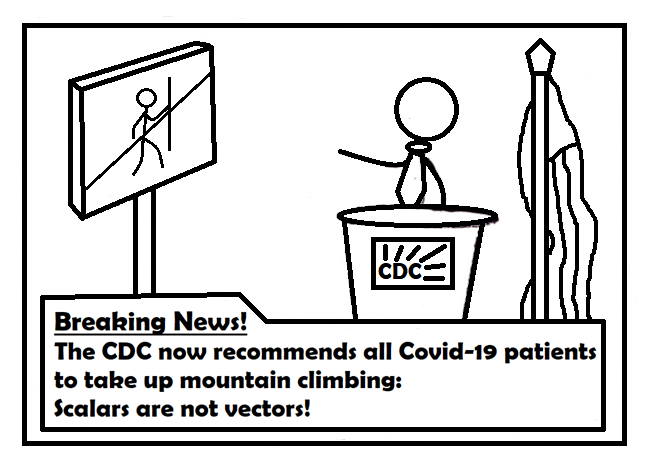
\includegraphics[scale=1]{Chapter2/images/cdc.png}}
%{\vspace{-10 pt}\hfill\footnotesize (Image contributed by Thayne Hansen)}\\

\pagebreak  %The Algebra and Geometry of Vectors
\begin{center} 
\emph{``If the world's a veil of tears, Smile till rainbows span it.'' -- Lucy Larcom}
\end{center}

\section{Vector Equations}\label{sec:span}
Linear combinations are the bread and butter of vectors. Algebraically speaking, this is what we do with vectors, that is, we combine some vectors to construct new vectors. While it is simple to take a list of vector, combine them, and see what pops out, the converse is not as simple. Given a list of vectors $\bb a_1, \bb a_2, \ldots, \bb a_n\in F^m$, can we determine if $\bb b\in F^m$ is a linear combination of these vectors? In other words, we seek to solve the vector equation:
\begin{equation}\label{eq:vectoreqn} x_1\bb a_1 + x_2\bb a_2 + \ldots + x_n\bb a_n = \bb b.\end{equation} In Equation \eqref{eq:vectoreqn}, note that the vectors $\bb a_1,\ldots, \bb a_n, \bb b$ are fixed and the variables are the scalars $x_1, x_2, \ldots, x_n\in F$. \\

To solve the vector equation \eqref{eq:vectoreqn}, suppose that the $i$th component of $\bb a_j$ is denoted $a_{ij}$, that is, 
\[\bb a_j = \mtx{c}{a_{1j} \\a_{2j} \\ \vdots\\ a_{mj}}.\] Likewise, let the $j$th component of $\bb b$ be $b_j$. Then Equation \eqref{eq:vectoreqn} becomes
\begin{eqnarray*} 
x_1\bb a_1 + x_2\bb a_2 + \ldots + x_n\bb a_n &=& \bb b\\
x_1\mtx{c}{a_{11} \\a_{21} \\ \vdots\\ a_{m1}} + x_2\mtx{c}{a_{12} \\a_{22} \\ \vdots\\ a_{m2}} + \ldots + x_n\mtx{c}{a_{1n} \\a_{2n} \\ \vdots\\ a_{mn}} &=& \mtx{c}{b_1\\b_2\\\vdots\\ b_m}\\
\mtx{c}{a_{11}x_1 \\a_{21}x_1 \\ \vdots\\ a_{m1}x_1} + \mtx{c}{a_{12}x_2 \\a_{22}x_2 \\ \vdots\\ a_{m2}x_2} + \ldots + \mtx{c}{a_{1n}x_n \\a_{2n}x_n \\ \vdots\\ a_{mn}x_n} &=& \mtx{c}{b_1\\b_2\\\vdots\\ b_m}\\
\mtx{c}{a_{11}x_1 + a_{12}x_2 + \ldots + a_{1n}x_n \\ a_{21}x_1 + a_{22}x_2 + \ldots + a_{2n}x_n \\ \vdots \\ a_{m1}x_1 + a_{m2}x_2 + \ldots + a_{mn}x_n}  &=& \mtx{c}{b_1\\b_2\\\vdots\\ b_m}\\
\end{eqnarray*} 

Examining this last equality of vectors reveals a system of linear equations, namely 
\begin{equation} \label{eq:linearsystem}
\begin{linear}
a_{11}x_1\ &+\ &a_{12}x_2\ &+\ &\ldots\ &+\ &a_{1n}x_n\ &=\ &b_1 \\ 
a_{21}x_1\ &+\ &a_{22}x_2\ &+\ &\ldots\ &+\ &a_{2n}x_n\ &=\ &b_2 \\ 
\vdots\quad &&\vdots\quad &&\ddots\ && \vdots\quad && \vdots\ \\ 
a_{m1}x_1\ &+\ &a_{m2}x_2\ &+\ &\ldots\ &+\ &a_{mn}x_n\ &=\ &b_m,
\end{linear}
\end{equation} whose augmented matrix is 
\[\mtx{rrrr|r}{ a_{11} & a_{12} & \ldots & a_{1n} & b_1 \\a_{21} & a_{22} & \ldots & a_{2n} & b_1 \\ \vdots & \vdots & \ddots & \vdots & \vdots \\ a_{m1} & a_{m2} & \ldots & a_{mn} & b_m   }.\] These two problems have the same solution set.\\

\begin{Thm} Let $\bb x = (x_1, x_2, \ldots, x_m)\in F^m$ be a vector over a field $F$. Then $\bb x$ is a solution to the vector equation \eqref{eq:vectoreqn} if and only if $\bb x$ is a solution to the linear system \eqref{eq:linearsystem}.
\end{Thm}

%NEW %UPDATE ROW OPERATIONS NOTATION
\begin{Exam} Let $\bb a_1 = \vr{1\\2\\3\\4}$, $\bb a_2 = \vr{1\\0\\0\\1}$, and $\bb a_3 = \vr{3\\0\\5\\7}$. Let $\bb b = \vr{-7 \\ 4 \\ -4 \\ -9}$. Is $\bb b$ a linear combination of $\bb a_1, \bb a_2, \bb a_3$?\\

To solve the vector equation, 
\[x_1\vr{1\\2\\3\\4} + x_2 \vr{1\\0\\0\\1} + x_3\vr{3\\0\\5\\7} = \vr{-7 \\ 4 \\ -4 \\ -9},\] we solve the linear system whose augmented matrix is 
\[\mtx{rrr|r}{1&1&3&-7\\2&0&0&4\\3&0&5&-4\\4&1&7&-9}.\] We next row reduce the matrix via the elementary row operations:
\[\mtx{rrr|r}{\fbox{1}&1&3&-7\\2&0&0&4\\3&0&5&-4\\4&1&7&-9}{\color{red}\begin{array}{c} \mbox{}\\ (\text{Row 2} - 2\text{Row 1}) \\ (\text{Row 3} - 3\text{Row 1}) \\ (\text{Row 4} - 4\text{Row 1})\end{array}} 
\sim  \mtx{rrr|r}{\fbox{1}&1&3&-7\\0&\fbox{$-2$}&-6&18\\0&-3&-4&17\\0&-3&-5&19}{\color{red}\begin{array}{c} \mbox{}\\ (-\frac{1}{2}\text{Row 2}) \\ \mbox{} \\ (\text{Row 4} - \text{Row 3})\end{array}}\]
\[\sim  \mtx{rrr|r}{\fbox{1}&1&3&-7\\0&\fbox{1}&3&-9\\0&-3&-4&17\\0&0&-1&2}{\color{red}\begin{array}{c} \mbox{}\\ \mbox{} \\ (\text{Row 3} + 3\text{Row 2}) \\ (-\text{Row 4})\end{array}} 
\sim  \mtx{rrr|r}{\fbox{1}&1&3&-7\\0&\fbox{1}&3&-9\\0&0&\fbox{5}&-10\\0&0&1&-2}{\color{red}\begin{array}{c} \mbox{}\\ \mbox{} \\ (\text{Interchange}) \\ (\text{Interchange})\end{array}} \]
\[\sim  \mtx{rrr|r}{\fbox{1}&1&3&-7\\0&\fbox{1}&3&-9\\0&0&\fbox{1}&-2\\0&0&5&-10}{\color{red}\begin{array}{c} \mbox{}\\ \mbox{} \\ \mbox{} \\ (\text{Row 4} - 5\text{Row 3})\end{array}}
\sim  \mtx{rrr|r}{\fbox{1}&1&3&-7\\0&\fbox{1}&3&-9\\0&0&\fbox{1}&-2\\0&0&0&0}
\]  This last matrix is in echelon form. We will continue to row reduced echelon form. 
\[\sim  \mtx{rrr|r}{\fbox{1}&1&3&-7\\0&\fbox{1}&3&-9\\0&0&\fbox{1}&-2\\0&0&0&0}{\color{red} \begin{array}{c} (\text{Row 1} - 3\text{Row 3})\\  (\text{Row 2} - 3\text{Row 3}) \\ \mbox{} \\ \mbox{}\end{array}} \sim  \mtx{rrr|r}{\fbox{1}&1&0&-1\\0&\fbox{1}&0&-3\\0&0&\fbox{1}&-2\\0&0&0&0}{\color{red} \begin{array}{c} (\text{Row 1} - \text{Row 2})\\  \mbox{} \\ \mbox{} \\ \mbox{}\end{array}} \sim \mtx{rrr|r}{\fbox{1}&0&0&2\\0&\fbox{1}&0&-3\\0&0&\fbox{1}&-2\\0&0&0&0}
\] Therefore, the solution is $(2,-3,-2)$. In fact, we see that 
\[2\vr{1\\2\\3\\4} - 3 \vr{1\\0\\0\\1} - 2\vr{3\\0\\5\\7} = \vr{-7 \\ 4 \\ -4 \\ -9}. \qedhere\]
\end{Exam}\vs

%NEW %UPDATE ROW OPERATIONS NOTATION
\begin{Exam} Let $\bb a_1 = \vr{1\\2\\3}$, $\bb a_2 =\vr{1\\0\\2}$, $\bb a_3 =\vr{2\\2\\4}$, $\bb a_4 = \vr{1\\1\\4}$, and $\bb b = \vr{4\\2\\1}$ be vectors over $\Z_5^3$. Is $\bb b$ a linear combination of $\bb a_1$, $\bb a_2$, $\bb a_3$, $\bb a_4$?\\

To solve the vector equation,
\[x_1\vr{1\\2\\3}+x_2\vr{1\\0\\2} + x_3\vr{2\\2\\4}+ x_4\vr{1\\1\\4} = \vr{4\\2\\1},\] we work with the augmented matrix
\[\mtx{cccc|c}{\fbox{1}&1&2&1&4 \\  2&0&2&1&2\\ 3&2&4&4&1}{\color{red} \begin{array}{c} \mbox{}\\  (\text{Row 2} - 2\text{Row 1}) \\ (\text{Row 3} - 3\text{Row 1}) \end{array}} 
\sim \mtx{cccc|c}{\fbox{1}&1&2&1&4 \\  0&\fbox{3}&3&4&4\\ 0&4&3&1&4}{\color{red} \begin{array}{c} \mbox{}\\  \mbox{} \\ (\text{Row 3} - 3\text{Row 2}) \end{array}}\]
\[\sim \mtx{cccc|c}{\fbox{1}&1&2&1&4 \\  0&\fbox{3}&3&4&4\\ 0&0&\fbox{4}&4&2}{\color{red} \begin{array}{c} \mbox{}\\  \mbox{} \\ (4\text{Row 3}) \end{array}}
\sim \mtx{cccc|c}{\fbox{1}&1&2&1&4 \\  0&\fbox{3}&3&4&4\\ 0&0&\fbox{1}&1&3}{\color{red} \begin{array}{c} (\text{Row 1} -2\text{Row 3})\\  (\text{Row 2} -3\text{Row 3}) \\ \mbox{} \end{array}}\]
\[\sim \mtx{cccc|c}{\fbox{1}&1&0&4&3 \\  0&\fbox{3}&0&1&0\\ 0&0&\fbox{1}&1&3}{\color{red} \begin{array}{c} \mbox{}\\  (2\text{Row 2}) \\ \mbox{} \end{array}}
\sim \mtx{cccc|c}{\fbox{1}&1&0&4&3 \\  0&\fbox{1}&0&2&0\\ 0&0&\fbox{1}&1&3}{\color{red} \begin{array}{c} (\text{Row 1} -\text{Row 2})\\  \mbox{} \\ \mbox{} \end{array}}\]
\[\sim \mtx{cccc|c}{\fbox{1}&0&0&2&3 \\  0&\fbox{1}&0&2&0\\ 0&0&\fbox{1}&1&3}\]

The resulting linear system is then 
\[\begin{linear}
x_1\ &&&+\ &2x_4\ &=\ &3\\
&x_2\ &&+\ &2x_4\ &=\ &0\\
&&x_3\ &+\ &x_4\ &=\ &3\\
\end{linear} \qRightarrow  \begin{linear}
x_1\ &=\ &3x_4\ &+\ &3\\
x_2\ &=\ &3x_4\ \\
x_3\ &=\ &4x_4\ &+\ &3\\
\end{linear}\] Therefore, there are five possibilities: $(3,0,3,0)$, $(1,3,2,1)$, $(4, 1, 1, 2)$, $(2, 4, 0, 3)$, and $(0, 2, 4, 4)$. This gives five possible linear combinations such as:
\[3\vr{1\\2\\3}+ 3\vr{2\\2\\4}  = \vr{1\\2\\3}+3\vr{1\\0\\2} + 2\vr{2\\2\\4}+ \vr{1\\1\\4} = \vr{4\\2\\1}.\qedhere \]
\end{Exam}

\begin{Def}\label{def:linearspan}
Given vectors $\bb v_1, \bb v_2, \ldots, \bb v_n \in F^m$, the \textbf{(linear) span} of $\bb v_1, \bb v_2, \ldots, \bb v_n$, denoted $\Span\{\bb v_1, \bb v_2, \ldots, \bb v_n\}$, is the set of all linear combinations of $\bb v_1, \bb v_2, \ldots, \bb v_n$ inside of $F^m$, that is, 
We say that a subset $S\subseteq F^m$ is \textbf{spanned} by $\bb v_1, \bb v_2, \ldots, \bb v_n$ if $S=\Span\{\bb v_1, \bb v_2, \ldots, \bb v_n\}$ and that $\{\bb v_1, \bb v_2, \ldots, \bb v_n\}$ is a \textbf{spanning set} for $S$. 
\end{Def}\vs

Asking whether a vector $\bb b \in \Span\{\bb a_1, \ldots, \bb a_n\}$ is equivalent to asking whether  there exists a solution $\bb b$ to the vector equation 
\[x_1\bb a_1 +  \ldots + x_n\bb a_n = \bb b.\] 

{\color{red} (These last two examples need to be replaced/updated).}
\begin{Exam} Let $\bb a_1 = \vr{1 \\ -2 \\ -5}$, $\bb a_2 = \vr{2 \\ 5 \\ 6}$, and $\bb b = \vr{7 \\ 4 \\ -3}$. Is $\bb b \in \Span\{\bb a_1, \bb a_2\}$?\\
As explained above, answering the question is equivalent to solving the vector equation $x_1\bb a_1 + x_2\bb a_2 = \bb b$. Likewise, this vector equation can be solved by row reduction on the augmented matrix $\mtx{rr|r}{ \bb a_1 & \bb a_2 & \bb b}$:
\[\mtx{rr|r}{1 & 2 & 7 \\ -2 & 5 & 4 \\ -5 & 6 & -3} \sim \mtx{rr|r}{1 & 2 & 7 \\ 0 & 9 & 18 \\ 0 & 16 & 32} \sim \mtx{rr|r}{1 & 2 & 7 \\ 0 & 1 & 2 \\ 0 & 1 & 2}  \sim \mtx{rr|r}{1 & 0 & 3 \\ 0 & 1 & 2 \\ 0 & 0 & 0}.\] Therefore, the solution is $x_1 = 3$ and $x_2 = 2$, that is, 
\[\bb b  = 3\bb a_1 + 2 \bb a_2 = 3\vr{1 \\ -2 \\ -5} + 2\vr{2 \\ 5 \\ 6} = \vr{7 \\ 4 \\ -3}.\qedhere\]
\end{Exam}\vs

\begin{Exam} Let $\bb a_1 = \vr{1 \\ -2 \\ 3}$, $\bb a_2 = \vr{5 \\ -13 \\ -3}$, and $\bb b = \vr{-3 \\ 8 \\ 1}$. Is $\bb b \in \Span\{\bb a_1, \bb a_2\}$?\\

Like above, we row reduce the augmented matrix $\mtx{rr|r}{ \bb a_1 & \bb a_2 & \bb b}$:
\[\mtx{rr|r}{1 & 5 & -3 \\ -2 & -13 & 8 \\ 3 & -3 & 1} \sim \mtx{rr|r}{1 & 5 & -3 \\ 0 & -3 & 2 \\ 0 & -18 & 10} \sim \mtx{rr|r}{1 & 5 & -3 \\ 0 & -3 & 2 \\ 0 & 0 & -2},\] which is now in echelon form. The third equation is $0=-2$, which implies that the system in inconsistent. Therefore, $\bb b\notin \Span\{\bb a_1, \bb a_2\}$
\end{Exam}


%SOME EXERCISES ARE DIRTY
%%%%%%%%%%%%%%%%%%% Exercises %%%%%%%%%%%%%%%%%%%
\startExercises{span}

\noindent For Exercises \ref{exer:vectoreqnstart}-\ref{exer:vectoreqnstop}, express the given system of equations as a vector equation.
\begin{enumerate}[!HW!, start=1]%, label=$\spadesuit$ \arabic*., ref=\arabic*]
\begin{multicols}{3}
\item\label{exer:vectoreqnstart} $\begin{linear} %Abby Allen
x_1\ &+\ &3x_2 &&&=\ &7\\
7x_1\ &+\ &6x_2\ &-\ &x_3\ &=\ &8\\
3x_1\ &+\ &x_2\ &+\ &2x_3\ &=\ &3
\end{linear}$ 
\itemspade $\begin{linear} %NEW
3x_1\ & +\ &7x_2\ &-\ &5x_3\ &=\ &-5\\
-x_1\ &-\ &2x_2\ &+\ &6x_3\ &=\ &4
\end{linear}$ 
\itemspade $\begin{linear} %NEW
-2x_1\ &+\ &6x_2\ &-\ &11x_3\ &=\ &6\\
x_1\ &-\ &2x_2\ &+\ &5x_3\ &=\ &-3\\
3x_1\ &-\ &19x_2\ &+\ &31x_3\ &=\ &-17
\end{linear}$
\end{multicols}
\begin{multicols}{3}
\item \label{exer:vectoreqnstop} 
$\begin{linear} 
x_1\ &+\ &2x_2\ &+\ &2x_3\ &=\ &1\\
3x_1\ &+\ &x_2\ & & &=\ &4\\
5x_1\ &+\ &2x_2\ &+\ &x_3\ &=\ &3
\end{linear}$ %Ashley Taylor
\end{multicols}
\end{enumerate}

\noindent For Exercises \ref{exer:combocheckstart}-\ref{exer:combocheckstop}, determine if $\bb b$ is a linear combination of the other vectors $\{\bb a_1, \bb a_2, \ldots\}$. If so, write $\bb b$ as a linear combination. The set of vectors $\{\bb a_1, \bb a_2,\ldots\}$ will be listed first, followed by the vector $\bb b$. Answers may vary. 
\begin{enumerate}[!HW!, label=$\spadesuit$ \arabic*., ref=\arabic*]
\begin{multicols}{2}
\item\label{exer:combocheckstart}  $\left\{\vr{-1\\3}, \vr{2\\-2}\right\}$,\ $\vr{1\\5}$ %anon
\item $\left\{\vr{-3\\-1\\1}, \vr{2\\2\\3}\right\}$,\ $\vr{5\\4\\3}$  %anon
\end{multicols}
\end{enumerate}
\begin{enumerate}[!HW!]
\begin{multicols}{2}
\itemspade $\left\{\vr{3\\-2\\1}, \vr{-2\\3\\-3}\right\}$, $\vr{1\\6\\-9}$ %anon
\item $\left\{\mtx{c}{1+i\\1-i\\3-2i}, \mtx{c}{1+2i\\1+i\\-2+i}\right\}$, $\mtx{c}{4+5i\\4-2i\\7-5i}$ %anon
\end{multicols}
\item\label{exer:combocheckstop} $\left\{\vr{1\\-1\\2\\1}, \vr{2\\1\\-1\\1}, \vr{-1\\2\\2\\-1}, \vr{1\\-1\\2\\2}\right\}$,\ $\vr{6\\3\\14\\8}$ %Christopher Newton
\end{enumerate}

\noindent For Exercises \ref{exer:spancheckstart}-\ref{exer:spancheckstop}, determine if $\bb b \in \Span\{\bb a_1, \bb a_2, \ldots\}$. If so, write $\bb b$ as a linear combination of the $\bb a_i$.  The set of vectors $\{\bb a_1, \bb a_2,\ldots\}$ will be listed first, followed by the vector $\bb b$. Answers may vary.
\begin{enumerate}[!HW!]
\item\label{exer:spancheckstart} $\left\{\vr{-4\\9\\6}, \vr{10\\6\\4}, \vr{7\\-12\\-8}\right\}$, $\vr{12\\4\\-6}$ %Kaden Allred
\end{enumerate}
\begin{enumerate}[!HW!, label=$\spadesuit$ \arabic*., ref=\arabic*]
\item\label{exer:spancheckstop} $\left\{\vr{1\\1\\2}, \vr{-2\\-1\\-2}, \vr{-1\\1\\2}\right\}$, $\vr{-4\\-1\\-2}$ %anon
\end{enumerate}

\begin{enumerate}[!HW!]
\itemspade For any list of vectors $\bb v_1,\ldots, \bb v_n$ in $F^m$, show that $\Span\{\bb v_1,\ldots, \bb v_n\}$ contains the zero vector.

\item Suppose that $\bb u_1, \bb u_2\in \Span\{\bb v_1, \bb v_2,\bb v_3\}$. Prove that $\Span\{\bb u_1, \bb u_2\}\subseteq \Span\{\bb v_1, \bb v_2, \bb v_3\}$.

\item Suppose that $\bb v_3 \in \Span\{\bb v_1, \bb v_2\}$. Prove that $\Span\{\bb v_1, \bb v_2\} = \Span\{\bb v_1, \bb v_2, \bb v_3\}$.

\item Prove that $\Span\{\bb v_1, \bb v_2\}=\Span\{\bb v_1, \bb v_1+\bb v_2\}$.

\item Suppose that $\bb u_1, \bb u_2,\ldots, \bb u _k\in \Span\{\bb v_1, \bb v_2, \ldots, \bb v_n\}$. Prove that $\Span\{\bb u_1, \bb u_2, \ldots, \bb u_k\}\subseteq \Span\{\bb v_1, \bb v_2,\ldots,  \bb v_n\}$.

\item Suppose that $\bb v_{n+1} \in \Span\{\bb v_1, \bb v_2,\ldots, \bb v_n\}$. Prove that $\Span\{\bb v_1, \bb v_2, \ldots, \bb v_n\} = \Span\{\bb v_1, \bb v_2, \ldots, \bb v_n, \bb v_{n+1}\}$.

\item \label{hw:changespanner} Let $c_i\in F$ be scalars such that $c_n\neq 0$. Prove that $\Span\{\bb v_1, \bb v_2, \ldots, \bb v_n\} = \Span\left\{\bb v_1, \bb v_2, \ldots, \bb v_{n-1}, \sum_{i=1}^n c_i\bb v_n\right\}.$

\item \label{hw:changespanner2}Suppose that $\bb u\in \Span\{\bb v_1, \bb v_2, \ldots, \bb v_n\}$ such that $\bb u\neq \bb 0$. Then there exists an $i$ such that \[\Span\{\bb v_1, \bb v_2,\ldots, \bb v_{i-1}, \bb v_i, \bb v_{i+1}, \ldots, \bb v\} = \Span\{\bb v_1, \bb v_2,\ldots, \bb v_{i-1}, \bb u, \bb v_{i+1}, \ldots, \bb v\}.\]
\end{enumerate}

%%%%%%%%%%%%%%%%%%% Footnotes %%%%%%%%%%%%%%%%%%%
\pagebreak%2.1 Vector Equations
\begin{center} 
\emph{``Some painters transform the sun into a yellow spot, others transform a yellow spot into the sun.''\\
-- Pablo Picasso}
\end{center}

\section{Matrix Equations}\label{sec:column}
\begin{Def} Let $A$ be  an $m\times n$ matrix and let $\bb x \in F^n$. Let the \textbf{column vectors} of $A$ be $\bb a_1, \bb a_2, \ldots, \bb a_n \in F^n$, that is, $A = \mtx{cccc}{\bb a_1 & \bb a_2 & \ldots & \bb a_n}$. Then the \textbf{product} $A\bb x$ is the linear combination of the column vectors of $A$ with coefficients corresponding to the entries of $\bb x$, that is, 
\begin{equation}\label{eq:matrixeqn} A\bb x =  \mtx{cccc}{\bb a_1 & \bb a_2 & \ldots & \bb a_n}\mtx{c}{x_1 \\ x_2 \\ \vdots \\ x_n} = x_1\bb a_1  + x_2\bb a_2 + \ldots + x_n\bb a_n.\end{equation}
\end{Def}\vs

Note that $A\bb x$ is only defined if the number of columns of $A$ is equal to the number of entries of $\bb x$.\\

\begin{Exam}\mbox{}
\begin{enumerate}
\item $\mtx{rrr}{1 & 2 & -3\\ 0 & -2 & 5}\vr{3 \\ 0 \\ 2} = 3\vr{1\\0} + 0\vr{2\\-2} + 2\vr{-3\\5} = \vr{3\\0} + \vr{0\\0} + \vr{-6\\10} = \vr{-3\\10}$.\\

\item $\mtx{rr}{2 & 0\\ -6 & 1 \\ 3 & 2}\vr{3\\5} = 3\vr{2\\-6\\3} + 5\vr{0\\1\\2} = \vr{6\\-18\\9} + \vr{0\\5\\10} = \vr{6\\-13\\19}$.
\end{enumerate}
\end{Exam}\vs

\begin{Thm} If $A$ is an $m\times n$ matrix, with column vectors $\bb a_1, \ldots, \bb a_n$, and if $\bb b\in F^m$, the matrix equation 
\begin{equation} A\bb x = \bb b\end{equation} has the same solution set as the vector equation 
\[x_1\bb a_1 + \ldots + x_n\bb a_n = \bb b\] which, in turn, has the same solution set as the system of linear equations whose augmented matrix is \[\mtx{rrr|r}{\bb a_1 & \ldots & \bb a_n & \bb b}.\]
\end{Thm}\vs

\begin{Exam} The solution set to the system of equation 
\[\left\{\begin{alignedat}{10}
& x_1\ &+\ &3x_2\ &-\ &7x_3\ &=\ &5&\\
& &-\ & 2x_2\ &+\ & 11x_3\ &=\ &3&
\end{alignedat}\right.\] is same as the solution set of the vector equation
\[x_1\vr{1\\0} + x_2\vr{3\\-2} + x_3\vr{-7\\11} = \vr{5\\3},\] which in turn has the same solution set as the matrix equation
\[\mtx{rrr}{1&3&-7\\0&-2&11}\vr{x_1\\x_2\\x_3} = \vr{5\\3}. \qedhere\]
\end{Exam}\vs 

\begin{Cor}\label{col} The equation $A\bb x = \bb b$ has a solution if and only if $\bb b$ is a linear combination of the column vectors of $A$.\end{Cor}\vs

\begin{Def} Let $\col(A)$ denote the set of all linear combinations of column vectors of $A$, which is called the \textbf{column space} of $A$. In particular, if $A = \mtx{cccc}{\bb a_1 & \bb a_2 & \ldots & \bb a_n}$, then $\col(A)  = \Span\{\bb a_1, \bb a_2, \ldots, \bb a_n\}$.\end{Def}\vs

According to \corref{col}, the equation $A\bb x = \bb b$ is consistent if and only if $\bb b\in \col(A)$.\\

\begin{Exam} Let $A = \mtx{rrr}{1 & 3 & 1\\ 2 & 4 & 4\\ 3 & 5 & 7}$. Compute the column space of $A$.\\

The quick response to this example would be to find a spanning set for the column space of $A$, but, by definition, a spanning set for a column space is never mysterious. Note that 
\[\col(A) = \Span\left\{\vr{1\\2\\3}, \vr{3\\4\\5}, \vr{1\\4\\7}\right\}.\] While we have technically computed the column space, that is, we have found a description of the set of vectors, it does not leave the decision question of whether a generic vector $\bb b = (b_1, b_2, b_3)$ belongs to $\col(A)$ well answered, which is really what we want to be able to do. To answer this question, we row reduce the augmented matrix
\begin{multline*}
\mtx{rrr|r}{1 & 3 & 1 & b_1\\ 2 & 4 & 4 & b_2\\ 3 & 5 & 7 & b_3} \sim \mtx{rrr|c}{1 & 3 & 1 & b_1\\ 0 & -2 & 2 & b_2-2b_1\\ 0 & -4 & 4 & b_3-3b_1} \sim \mtx{rrr|c}{1 & 3 & 1 & b_1\\ 0 & 1 & 1 & b_1-\frac{1}{2}b_2\\ 0 & 1 & -1 & \frac{1}{4}(3b_1-b_3)}
\sim \mtx{rrr|c}{1 & 3 & 1 & b_1\\ 0 & 1 & 1 & b_1-\frac{1}{2}b_2\\ 0 & 0 & 0 & -\frac{1}{4}b_1+\frac{1}{2}b_2-\frac{1}{4}b_3}
\end{multline*}
Therefore, the above equation is consistent if and only if $-\frac{1}{4}b_1+\frac{1}{2}b_2-\frac{1}{4}b_3 = 0$. Therefore, Now, there exists plenty of choices of $\bb b$ such that this equation does not hold. Hence, $A\bb x = \bb b$ is not consistent for all $\bb b$. \[\col(A) = \{\bb b \in \R^3\mid b_1-2b_2+b_3=0\}. \qedhere\] 
\end{Exam}\vs

Generalizing the principles seen in the previous example, for any $n\times n$ matrix $A$, the equation $A\bb x = \bb b$ has a solution for all $\bb b$ if and only if $A$ has a pivot in each row, in which case the solution must be unique.\\

Let $A$ be an $(m\times n)$ matrix and let $\bb x\in F^n$. Then the rule $\bb x \mapsto A\bb x$ is a transformation called a \emph{matrix transformation}.\\


\begin{Thm} Let $A$ be an $m\times n$ matrix and let $\bb u, \bb v \in F^n$. Let $c\in F$. Then $A(\bb u+\bb v) = A\bb u+A\bb v$ and $A(c\bb u) = c(A\bb u)$. In particular, multiplication by a matrix is a linear transformation.\end{Thm}\vs

Let $A$ be an $m\times n$ matrix with column vectors $\bb a_1, \ldots, \bb a_n$. Let $A  = \mtx{r}{a_{ij}}$, that is, let $a_{ij}$ denote the entry of $A$ in the $(i,j)$ position. Let $\bb x\in F^n$. Then 
\begin{eqnarray*}A\bb x &=& \mtx{rrrr}{\bb a_1 & \bb a_2 & \ldots & \bb a_n}\mtx{c}{x_1\\ x_2 \\ \vdots\\x_n} = x_1\bb a_1 + \ldots + x_n\bb a_n = x_1\mtx{c}{a_{11}\\ a_{21} \\ \vdots \\ a_{m1}} +  x_2\mtx{c}{a_{12}\\ a_{22} \\ \vdots \\ a_{m2}} + \ldots +  x_n\mtx{c}{a_{1n}\\ a_{2n} \\ \vdots \\ a_{mn}}\\ &=& \mtx{c}{x_1a_{11}\\ x_1a_{21} \\ \vdots \\ x_1a_{m1}} +  \mtx{c}{x_2a_{12}\\ x_2a_{22} \\ \vdots \\ x_2a_{m2}} + \ldots +  \mtx{c}{x_na_{1n}\\ x_na_{2n} \\ \vdots \\ x_na_{mn}} = \mtx{c}{x_1a_{11} + x_2a_{12} + \ldots + x_na_{1n}\\ x_1a_{21} + x_2a_{22} + \ldots + x_na_{2n}\\\vdots\\  x_1a_{m1} + x_2a_{m2} + \ldots + x_na_{mn}}.
\end{eqnarray*} That is \begin{equation} A\bb x = \mtx{c}{x_1a_{11} + x_2a_{12} + \ldots + x_na_{1n}\\ x_1a_{21} + x_2a_{22} + \ldots + x_na_{2n}\\\vdots\\  x_1a_{m1} + x_2a_{m2} + \ldots + x_na_{mn}}.\end{equation} This formula often is easier to compute than the original definition of $A \bb x$.\\

\begin{Exam} Let $A = \mtx{rr}{  0 & -2 \\ 1 & -3 \\ 2 & -3}$ and define a transformation $T : \R^2 \to \R^3$ by $T(\bb x) = A\bb x$. Then 
\[T(\bb x) = A\bb x = \mtx{rr}{ 0 & -2 \\ 1 & -3 \\ 2 & -3}\vr{x_1\\x_2}.\]\vs

\begin{enumerate}
\item Let $\bb u = \vr{3\\-1}$. Compute $T(\bb u)$.\\

\[T(\bb u) = A\bb u = \vr{0(3) - 2(-1) \\ 1(3) - 3(-1) \\ 2(3) - 3(-1)} = \vr{2\\6\\9}.\]

\item Find an $\bb x\in \R^2$ whose image under $T$ is $\bb b = \vr{-8\\-7\\-2}$.\\

We need an $x_1$ and $x_2$ such that \[\mtx{rr}{  0 & -2 \\ 1 & -3 \\ 2 & -3}\vr{x_1\\x_2} = \vr{-8\\-7\\-2}.\] By row reduction, we solve the corresponding linear system:
\[\mtx{rr|r}{ 0 & -2 & -8 \\ 1 & -3 & -7 \\ 2 & -3 & -2} \sim \mtx{rr|r}{ 1 & -3 & -7 \\ 0 & -2 & -8 \\  2 & -3 & -2} \sim \mtx{rr|r}{ 1 & -3 & -7 \\ 0 & -2 & -8 \\  0 & 3 & 12} \sim 
\mtx{rr|r}{ 1 & -3 & -7 \\ 0 & 1 & 4 \\  0 & 1 & 4}\sim \mtx{rr|r}{ 1 & -3 & -7 \\ 0 & 1 & 4 \\  0 & 0 & 0}
\sim \mtx{rr|r}{ 1 & 0 & 5 \\ 0 & 1 & 4 \\  0 & 0 & 0}.\] Let $\bb x = \vr{5\\4}$. Then, $T(\bb x) = \bb b$. In fact, $\bb x$ is the only vector whose image under $T$ is $\bb b$. \hfill$\qedhere$
\end{enumerate}
\end{Exam}

%%%%%%%%%%%%%%%%%%% Exercises %%%%%%%%%%%%%%%%%%%
\startExercises{column}

\noindent For Exercises \ref{true:columnstart}-\ref{true:columnstop}, determine with the statement is true or false. If false, correct the statement so that it is true.
\begin{enumerate}[!HW!, start=1]
\item\label{true:columnstart}\label{true:columnstop} A homogeneous linear system can be written as $A\bb x = 0$, where $A$ is the $m\times n$ coefficient matrix, $\bb x\in F^n$, and $0$ is a scalar. %Da Huo
\end{enumerate}

\noindent For Exercises \ref{exer:matrixvectorproductrealstart}-\ref{exer:matrixvectorproductrealstop}, compute the matrix-vector product. 
\begin{enumerate}[!HW!]
\begin{multicols}{2}
\item\label{exer:matrixvectorproductrealstart} $\mtx{rrr}{4&5&2\\0&-1&3\\2&1&1}\vr{1\\4\\3}$ %Alexis Borell
\itemspade $\mtx{rrr}{3&-1&2\\4&3&7\\-2&1&5}\vr{2\\-3\\1}$
\end{multicols}
\end{enumerate}
\begin{enumerate}[!HW!, label=$\spadesuit$ \arabic*., ref=\arabic*]
\begin{multicols}{2}
\itemspade $\mtx{cr}{1+2i&-1+3i\\0&3+4i}\vr{7+i\\-2-i}$
\item\label{exer:matrixvectorproductrealstop} $\mtx{ccccc}{1&1&1&0&0\\0&1&0&1&0\\1&0&0&0&1}\vr{1\\1\\0\\0\\1}\pmod 2$
\end{multicols}
\end{enumerate}

\noindent For Exercises \ref{exer:mtxeqnlinearsystemstart}-\ref{exer:mtxeqnlinearsystemstop}, express the given matrix equation as a system of equations.
\begin{enumerate}[!HW!, resume, label=$\spadesuit$ \arabic*., ref=\arabic*]
\begin{multicols}{2}
\item\label{exer:mtxeqnlinearsystemstart} \mbox{$\mtx{rrrr}{4&1&-3 &0\\ 0 &4&-12 &1 \\ 2&-3&-1&5}\vr{x_1\\x_2\\x_3\\x_4} \equiv \vr{1\\0\\2} \pmod 5$}
\itemspade $\mtx{rr}{1 & 2 \\ 3 & 4\\ -1 & -2 \\ 4&5}\vr{x\\y} = \vr{2\\0\\2\\-9}$
\end{multicols}
\end{enumerate}
\begin{enumerate}[!HW!]
\item\label{exer:mtxeqnlinearsystemstop} $\mtx{rrrr}{21&27&17&-32\\4&42&6&19\\103&-72&17&-8\\2&11&-10&13}\vr{x\\y\\z\\w}=\vr{12\\-6\\15\\1}$ %anon
\end{enumerate}

\noindent For Exercises \ref{exer:mtxeqnsolverealstart}-\ref{exer:mtxeqnsolverealstop}, solve the  matrix equation.
\begin{enumerate}[!HW!]
\begin{multicols}{2}
\item \label{exer:mtxeqnsolverealstart} $\mtx{rrr}{1&2&3\\-1&-1&-3\\-1&-2&-2}\vr{x_1\\x_2\\x_3}=\vr{10\\-8\\-9}$ %Jianhe Yu
\itemspade $\mtx{rrr}{4&4&2\\-4&-3&-2\\-4&-3&1}\vr{x_1\\x_2\\x_3} = \vr{12\\-3\\3}$
\end{multicols}
\begin{multicols}{2}
\itemspade $\mtx{rr}{1&0\\2&5\\3&-2}\vr{x_1\\x_2} = \vr{1\\3\\0}$
\item $\mtx{ccc}{1-i&1&1+i\\1&i&-i\\3+i&2&3i}\vr{x_1\\x_2\\x_3}=\mtx{c}{7\\3i\\11+7i}$ %Jianhe Yu
\end{multicols}
\begin{multicols}{2}
\itemspade $\mtx{rrr}{1&4&3\\4&3&4\\3&4&3}\vr{x_1\\x_2\\x_3} \equiv \vr{4\\3\\2} \pmod 5$
\item $\mtx{rrr}{0&1&2\\2&1&0\\1&0&2}\vr{x_1\\x_2\\x_3}\equiv \vr{1\\1\\0} \pmod 3$ %Seth Palmer
\end{multicols}
\begin{multicols}{2}
\item $\mtx{rrrr}{1&0&1&2\\2&2&0&0\\0&0&1&2}\vr{x_1\\x_2\\x_3\\x_4}\equiv \vr{1\\1\\1} \pmod 3$ %Mitchel Zufelt
\item\label{exer:mtxeqnsolverealstop} $\mtx{rrrr}{1&1&1&1\\1&1&0&1\\1&1&1&0\\0&1&0&1}\vr{x_1\\x_2\\x_3\\x_4}\equiv \vr{0\\1\\0\\0}\pmod 2$ %Jianhe Yu
\end{multicols}
\end{enumerate}

\noindent For Exercises \ref{exer:mtxtransformstart}-\ref{exer:mtxtransformstop}, use the transformation $T : \R^4 \to \R^2$ given by the rule:
\[T(x_1, x_2, x_3, x_4) = \mtx{rrrr}{2&-1&0&3 \\ 0&6&-2&1}\vr{x_1\\x_2\\x_3\\x_4}.\]
\begin{enumerate}[!HW!, resume, label=$\spadesuit$ \arabic*., ref=\arabic*]
\begin{multicols}{2}
\item\label{exer:mtxtransformstart} Compute $T(1, 0, 0, 1)$ and $T(1, 2, 3, 4)$.\\
\item\label{exer:mtxtransformstop} Find $\bb x$ such that $T(\bb x) = (1,2)$.\\
\end{multicols}
\end{enumerate}

\begin{enumerate}[!HW!]
\item It can be shown that $(4,3,2,1)$ is the unique solution to the system of linear equations %Samuel Andersen
\[\begin{linear}
11x_1\ &+\ &9x_2\ &+\ &10x_3\ &+\ &14x_4\ &=\ &105\\
9x_1\ &+\ &4x_2\ &+\ &5x_3\ &+\ &9x_4\ &=\ &67\\
11x_1\ &+\ &12x_2\ &+\ &13x_3\ &+\ &17x_4\ &=\ &123\\
7x_1\ &+\ &2x_2\ &+\ &5x_3\ &+\ &7x_4\ &=\ &51&.
\end{linear}\] With this knowledge, QUICKLY solve the matrix equation \[\mtx{rrrr}{11&9&10&14\\9&4&5&9\\11&12&13&17\\7&2&5&7}\vr{x_1\\x_2\\x_3\\x_4} = \vr{105\\67\\123\\51}.\] Why were you able to solve it so quickly?
\end{enumerate}
%%%%%%%%%%%%%%%%%%% Footnotes %%%%%%%%%%%%%%%%%%%
\pagebreak%2.2 Matrix Equations
\begin{center} 
\emph{``All mankind... being all equal and independent, no one ought to harm another in his life, health, liberty or possessions.'' -- John Locke}
\end{center}

\section{Linear Independence}\label{sec:independence}
\begin{Def} A set of vectors $\{\bb a_1, \bb a_2, \ldots, \bb a_n\}\subseteq F^m$ is said to be \textbf{linearly independent} if the vector equation 
\[x_1\bb a_1 + x_2\bb a_2 + \ldots + x_n\bb a_n =  \bb 0\] has only the trivial solution. Otherwise, the set is said to be \textbf{linearly dependent}. 
\end{Def}

In other words, a set of vectors is linearly dependent if there exists some weights $c_1, c_2, \ldots, c_n$, with at least one not zero, such that 
\[c_1\bb a_1 + c_2\bb a_2 + \ldots + c_n\bb a_n = \bb 0.\] The previous equation is then called a \textbf{linear dependence relation}.\\

Expressed another way, suppose $A = \mtx{rrrr}{ \bb a_1 & \bb a_2 & \ldots & \bb a_n}$, then $\{\bb a_1, \ldots, \bb a_n\}$ is linearly independent if and only if $A\bb x = \bb 0$ has no nontrivial solution, since 
\[A\bb x = \mtx{rrrr}{ \bb a_1 & \bb a_2 & \ldots & \bb a_n}\mtx{c}{x_1 \\ x_2 \\ \vdots \\ x_n} = x_1\bb a_1 + x_2\bb a_2 + \ldots + x_n\bb a_n =  \bb 0.\] The set $\{\bb a_1, \ldots, \bb a_n\}$ is linearly dependent if and only if $A\bb x = \bb 0$ has a nontrivial solution.\\

\begin{Exam}\label{exam:lineardependent} Let $\bb v_1 = \vr{1 \\ 2 \\3}$, $\bb v_2 = \vr{3\\1\\-2}$, and $\bb v_3 = \vr{-3\\4\\13}$.\\

\begin{enumerate}
\item Determine if the set $\{\bb v_1, \bb v_2, \bb v_3\}$ is linearly independent.\\

To determine if the set is linearly independent, it suffices to compute the echelon form of the corresponding homogeneous system. In fact, the final row of zeros is irrelevant.
\[\mtx{rrr}{1&3&-3\\2&1&4\\3&-2&13} \sim \mtx{rrr}{1&3&-3\\0&-5&10\\0&-11&22 } \sim \mtx{rrr}{1&3&-3\\0&1&-2\\0&1&-2 }\sim \mtx{rrr}{1&3&-3\\0&1&-2\\0&0&0 }.\] Thus, $x_3$ is a free variable of the system, which implies that the homogeneous equation $A\bb x = \bb 0$ does have a nontrivial solution. Therefore, $\{\bb v_1, \bb v_2, \bb v_3\}$ is linearly dependent.\\

\item Find a linear dependence relation among $\bb v_1$, $\bb v_2,$ and $\bb v_3$.

To determine a dependence relation, we finish the row reduction from above.
\[\mtx{rrr}{1&3&-3\\0&1&-2\\0&0&0 } \sim \mtx{rrr}{1&0&3\\0&1&-2\\0&0&0 }.\] Therefore, 
\[\left\{\begin{alignedat}{100}
&x_1\ && & +\ &3x_3\ &=\ &0&\\
&&& x_2\ & -\ &2x_3\ &=\ &0&\\
&&&&&0\ &=\ &0&
\end{alignedat}\right. 
\] Thus, $\bb x = \vr{x_1\\x_2\\x_3} = \vr{-3x_3\\2x_3 \\ x_3} = x_3\vr{-3\\2\\1}$. Thus, $-3\bb v_1 +2 \bb v_2 + \bb v_3 = \bb 0$ (corresponding to $x_3=1$). Of course, there are infinitely many dependence relations. For example, $-15\bb v_1 + 10\bb v_2 + 5\bb v_3 = \bb 0$ (corresponding to $x_3 = 5$).\\

We also note that we have shown that $\bb v_3\in \Span\{\bb v_1, \bb v_2\}$ since $-3\bb v_1 +2 \bb v_2 + \bb v_3 = \bb 0$ implies $\bb v_3 = 3\bb v_1 - 2\bb v_2$. This observation is always the case for linear dependence.\hfill$\qedhere$
\end{enumerate}
\end{Exam}\vs

\begin{Exam} Determine if the columns of the matrix $A = \mtx{rrr}{1&-1&-1\\-1&2&4\\2&-4&-7}$ are linearly independent.\\

It suffices to show that $A\bb x = \bb 0$ has no nontrivial solutions, that is, that an echelon form of $A$ has no zero rows.
\[\mtx{rrr}{\fbox{$1$}&-1&-1\\-1&2&4\\2&-4&-7}\sim \mtx{rrr}{\fbox{$1$}&-1&-1\\0&\fbox{$1$}&3\\0&-2&-5}\sim \mtx{rrr}{\fbox{$1$}&-1&-1\\0&\fbox{$1$}&3\\0&0&\fbox{$1$}}.\] Therefore, the columns of $A$ are linearly independent.
\end{Exam}\vs

These examples illustrate an important point: a set of vector is linearly dependent if and only if the corresponding homogeneous linear system has a free variable. In other words, a set of vectors is linearly independent if and only if the associated coefficient matrix has a pivot in each column.\\

The following properties provided, in some cases, a quick test to determine the linear independence or dependence of a set of vectors.\\

\begin{Thm}\label{prop:indTest1}\mbox{}
\begin{enumerate}
\item If a set contains a linearly dependent subset, then the set itself is linearly dependent.\\
\item The set $\{\bb v\}$ is linearly independent if and only if $\bb v \neq \bb 0$.\\
\item If a set $S \subseteq F^n$ contains the zero vector, then $S$ is linearly dependent.\\
\item A set $S = \{\bb v_1, \ldots, \bb v_p\}\subseteq F^n$  for $p>1$ is linearly dependent if and only if at least one of the vectors of $S$ is a linear combination of the others.\\
\item The set $\{\bb u, \bb v\}$ is linearly independent if and only if neither vector is a multiple of the other, that is $\bb v \neq c\bb u$ nor $\bb u \neq c\bb v$ for any $c\in F$.\\
\item Suppose $S = \{\bb v_1, \ldots, \bb v_p\} \subseteq F^n$. If $p > n$, then $S$ is linearly dependent.\\
\end{enumerate}
\end{Thm}
\begin{proof}\mbox{}
\begin{enumerate}
%\item This was addressed above.\\
\item Suppose $S$ is linearly dependent and $S\subseteq T$. Then set every vector in $T$ which is not in $S$ to have weight zero. Then a dependence relation on $S$ becomes a dependence relation on $T$.\\
\item Note that  $c\bb v = \bb 0$ if and only if $c = 0$ or $\bb v = \bb 0$.\\
\item It follows from the previous two parts. \\%Set the weight of the zero vector to one and set the weight of any other vector in $S$ to zero. This gives a dependence relation.
\item Suppose first that $S$ is linearly dependent and \[c_1\bb v_1 + \ldots + c_p\bb v_p = \bb 0\] is a dependence relation. Now there exists some $j$ such that $c_j\neq 0$. Without the loss of generality, we may suppose that $j=p$. Then 
\begin{eqnarray*}
c_1\bb v_1 + \ldots + c_{p-1}\bb v_{p-1} &=& -c_p\bb v_p\\
\frac{c_1}{-c_p}\bb v_1 + \ldots + \frac{c_{p-1}}{-c_p}\bb v_{p-1} &=& \bb v_p.
\end{eqnarray*} So, $\bb v_p \in \Span\{\bb v_1, \ldots \bb v_{p-1}\}$. \\

Conversely, if $v_p = c_1\bb v_1 + \ldots + c_{p-1}\bb v_{p-1}$, then \[c_1\bb v_1 + \ldots + c_{p-1}\bb v_{p-1} - v_p = \bb 0\] is a dependence relation, that is, $\{\bb v_1, \ldots, \bb v_p\}$ is linearly dependent.

\item This follows immediately from the previous part when $p=2$. \\ %Suppose that $\{\bb u, \bb v\}$ is linearly dependent. If $a\bb u + b\bb v = \bb 0$, then $a\bb u = - b\bb v$. If this is a dependence relation, then $a$ or $b$ is nonzero. Without the loss of generality, suppose that $a\neq 0$. Then $\bb u  = -\frac{b}{a}\bb v$. The converse is similar.

\item Let $A = \mtx{rrr}{\bb v_1 & \ldots & \bb v_p}$. Then $A$ is an $n\times p$ matrix and the equation $A\bb x = \bb 0$ corresponds to an under-determined system of $n$ equation with $p$ unknowns. Thus, the system has a free variable by \thmref{prop:1.1determine}, which implies the linear dependence of the column vectors. %If $p > n$, then there are more variables than equations. So there must be a free variable (Think about what would happen after you row reduced this matrix). Hence, $A\bb x = \bb 0$ has a nontrivial solution and the columns are linearly dependent.
\hfill$\qedhere$
\end{enumerate}
\end{proof}\vs

\begin{Exam} Determine by inspection if the given sets are linearly independent.
\begin{enumerate}
\begin{multicols}{2}
\item $\left\{\vr{7\\1\\6}, \vr{9\\0\\2}, \vr{4\\2\\5}, \vr{3\\1\\9}\right\}$.\\

This set of vectors is linearly dependent because any set of 4 vectors in $\R^3$ must be dependent.\\
\end{multicols}
\begin{multicols}{2}
\item $\left\{\vr{3\\1\\5}, \vr{0\\0\\0}, \vr{2\\1\\7}\right\}$.\\

This set of vectors is linearly dependent because it contains the zero vector.\\
\end{multicols}\pagebreak
\begin{multicols}{2}
\item $\left\{\vr{15\\0\\20\\-5}, \vr{-12\\0\\-16\\4}\right\}$.

This set of vectors is linearly dependent because the second vector is just $(-5/4)$ times the first vector.\vfill\hfill$\qedhere$
\end{multicols} 
\end{enumerate}
\end{Exam}

%%%%%%%%%%%%%%%%%%% Exercises %%%%%%%%%%%%%%%%%%%
\startExercises{independence}
\noindent For Exercises \ref{true:independencestart}-\ref{true:independencestop}, determine with the statement is true or false. If false, correct the statement so that it is true.
\begin{enumerate}[!HW!,start=1]
\item\label{true:independencestart} If a set $S\subseteq F^n$ contains the zero vector, then $S$ is linearly independent. %Carson Blickenstaff
\item If a set contains a linearly dependent subset, then the set itself is linearly dependent. %Carson Blickenstaff
\item The set $\{\bb u, \bb v\}$ is linearly independent if and only if neither vector is a multiple of the other, that is, $\bb v \neq c\bb u$ and $\bb u \neq c\bb v$ for any $c\in F$. %Carson Blickenstaff
\item Suppose $S=\{\bb v_1,\ldots, \bb v_p\}\subseteq F^n$. If $p>n$, then $S$ is linearly dependent.  %Carson Blickenstaff
\item The set $\{\bb v\}$ is linearly independent if and only if $\bb v\neq 0$.  %Carson Blickenstaff
\item\label{true:independencestop} A set $S$ of two or more vectors is linearly dependent if and only if at least one of the vectors in $S$ is a linear combination of the others.\\  %Carson Blickenstaff
\end{enumerate}

\noindent QUICK! For Exercises \ref{exer:quickLIrealstart}-\ref{exer:quickLIrealstop}, determine whether of the set of vectors is linearly independent or dependent using \thmref{prop:indTest1} in LESS THAN 10 SECONDS! Justify your quick response. 
\begin{enumerate}[!HW!, label=$\spadesuit$ \arabic*., ref=\arabic*]
\begin{multicols}{2}
\item\label{exer:quickLIrealstart} $\left\{\vr{1\\2\\3}, \vr{0\\1\\4}, \vr{0\\0\\0}\right\}$
\item $\left\{\mtx{c}{1\\i}, \vr{1\\0}\right\}$
\end{multicols}
\begin{multicols}{2}
\item $\left\{\vr{1\\2\\3\\4}\right\} \pmod{11}$
\item\label{exer:quickLIrealstop} \mbox{$\left\{\vr{1\\0\\1\\1}, \vr{0\\0\\0\\1}, \vr{1\\1\\1\\1}, \vr{0\\1\\1\\0}, \vr{1\\0\\0\\1}\right\} \pmod 2$}
\end{multicols}
\end{enumerate}

\noindent For Exercises \ref{exer:LIrealstart}-\ref{exer:LIrealstop}, determine if the set of vectors is linearly independent or dependent. If linearly dependent, provide a nontrivial dependency relation. 
\begin{enumerate}[!HW!]
\begin{multicols}{2}
\item\label{exer:LIrealstart} $\left\{\vr{1\\0\\2},\vr{2\\2\\4},\vr{3\\6\\5}\right\}$ %Abby Allen
\itemspade $\left\{\vr{1\\-1\\3},\vr{2\\-2\\6},\vr{-2\\3\\-2}\right\}$
\end{multicols}
\begin{multicols}{2}
\itemspade $\left\{\vr{1\\-2\\-1\\-1}, \vr{-1\\2\\2\\4}, \vr{2\\-3\\-3\\2}\right\}$
\item $\left\{\vr{2\\4\\6},\vr{1\\3\\2},\vr{4\\1\\3}\right\}$ %Hailey Checketts
\end{multicols}
\begin{multicols}{2}
\itemspade $\left\{\mtx{r}{i\\1\\-i}, \mtx{c}{2\\1-2i\\-1+i}, \mtx{c}{0\\i\\i}\right\}$
\itemspade $\left\{\vr{1\\3\\1}, \vr{1\\0\\0},\vr{1\\2\\2}\right\} \pmod 5$
\end{multicols}
\end{enumerate}
\begin{enumerate}[!HW!,label=$\spadesuit$ \arabic*., ref=\arabic*]
%\begin{multicols}{2}
\item%spade
\label{exer:LIrealstop} $\left\{\vr{1\\2\\0\\1}, \vr{2\\6\\6\\4}, \vr{6\\5\\1\\1}, \vr{0\\5\\4\\4}\right\} \pmod 7$
%\end{multicols}
\end{enumerate}

%%%%%%%%%%%%%%%%%%% Footnotes %%%%%%%%%%%%%%%%%%%
\pagebreak%2.3 Linear Independence
\begin{center} 
\emph{``Space is an inspirational concept that allows you to dream big.'' -- Peter Diamandis}
\end{center}

\section{Affine Geometry}\label{sec:flat}
For any field, there is a limited amount of geometry, called \textbf{affine geometry}, we can attach to the vector space $F^n$ by mimicking geometric structures from $\R^n$.\\

\begin{Def} Let $F^n$ be a vector space. Then a \textbf{flat} (or \textbf{affine set}) is a subset of $F^n$ which is congruent to $F^m$ for some $0\le m\le n$. Equivalently, flats are solution sets of linear systems (vector equations, matrix equations, etc.).
\end{Def}\vs

To describe flats, e.g., points, lines, planes, we present two recursive constructions: \emph{Top-Down} or \emph{Bottom-Up}. The \emph{Top-Down} approach is to start with a single non-zero, linear equation $a_{1,1}x_1+\ldots + a_{1,n}x_n=b_i$. The solution set of this linear equation forms a special kind of flat, called  a \textbf{hyperplane}. For example, $ax+by+cz=d$ defines a \emph{plane} in $\R^3$. By plane, we mean something that ``looks'' like $\R^2$ inside of $\R^n$. In general, a \emph{plane} over $F^n$ should be a subset that ``looks'' like $F^2$. The solution set to this $1\times n$ system should have $n-1$ free variables. Generally speaking, we view a hyperplane in $F^n$ as an affine set that ``looks'' likes $F^{n-1}$ in $F^n$. \\

Next, consider a linear system that contains the above linear equation and a second one $a_{2,1}x_1 + \ldots + a_{2,n}x_n=b_2$. The solution set to this $2\times n$ linear system is geometrically the intersection of the two hyperplanes, for example, two distinct planes intersecting in $\R^3$ form a \emph{line}. By line, we mean something that looks like $\R^1=\R$ inside of $\R^n$. In general, a \emph{line} over $F^n$ should be a subset that ``looks'' like $F^1=F$. If the equations are linearly independent, then this $2\times n$ system will have $n-2$ free variables. Hence, we view an intersection of two hyperplanes in $F^n$ as an affine set that ``looks'' likes $F^{n-2}$ in $F^n$. \\

Continuing in this fashion of expanding the linear system by adding new linear equations while maintaining linear independence, the $m\times n$ linear system will have  $n-m$ free variables and the flat will resemble $F^{n-m}$. This continues until $m=n$ and the intersection of hyperplanes is just a point, which resembles $F^0=\{\bb 0\}$. In this case, there are no free variables to the linear system. This is, of course, only true if the set of linear equations is linearly independent; if linearly dependent, then at least one equation is a linear combination of the rest and its removal does not change the flat one bit. That is, the inclusion of a linear combination of equations already in the system offers no restriction on the solution set whatsoever, and this equation is frankly redundant to the linear system. This summarizes the \emph{Top-Down} approach to affine sets.\\

The ``shape'' of the flat, that is, the parameter $p$ for which the affine set resembles $F^p$, appears to be determined by the number of free variables in the linear system. The \emph{Bottom-Up} approach to flats is to adjoin more and more free variables until the flat has the right ``shape.''\\

A \textbf{point} in $F^n$ is the solution to the vector equation \[ \bb x = \bb x_0,\] where $\bb x$ is a variable vector and $\bb x_0$ is a fixed vector. So a point in $F^n$ is just a vector, that is, $P = \bb x_0$. It is also a translation of the empty span $\Span\{\} = \{\bb 0\} = F^0$.\\

A \textbf{line} in $F^n$, call it $\ell$,  is the translation of the span of a single vector $\bb v$, which acts as the direction or slope of the line. If $\bb x_0$ is a point on $\ell$, then $\ell$ is the solution set to the vector equation
\[ \bb x = \bb{x_0} + t\bb v.\] 

Similarly, a \textbf{plane} in $F^n$, call it $\mathcal{P}$, is a translation of a span of two linearly independent vectors, that is, a translation of $\Span\{\bb u, \bb v\}$. Then $\mathcal{P}$ is the solution set to the vector equation
\[ \bb x = \bb{x_0} + s\bb u + t\bb v,\]
where vectors $\bb u,\ \bb v\in F^n$, $\{\bb u, \bb v\}$ is linear independent, and $\bb{x_0}$ is on $\mathcal{P}$.\\

By allegory, we can construct higher flats by increasing the number of linearly independent vectors in the linear combination associated with the vector equation, that is, we increase the number of linearly independent vectors in the spanning set, the so-called \textbf{spanners} of the flat. For example, a hyperplane in $F^4$ is the set of solutions to the vector equation 
\[\bb x = \bb x_0 + r\bb u + s\bb v + t\bb w,\] where $\{\bb u, \bb v, \bb w\}\subseteq F^4$ is linearly independent. More generally, an $m$-flat is the solution set to the vector equation
\begin{equation}\label{eq:flatvectorform} \bb x = \bb x_0 + \sum_{i=1}^m t_i\bb v_i, \end{equation} where $\{\bb v_1, \bb v_2, \ldots, \bb v_m\} \subseteq F^n$ is a linearly independent set of vectors. Equation \eqref{eq:flatvectorform} is called the \textbf{vector form of the flat}. Each component in this vector equation is a linear equation in its own right. The system of linear equations associated to this vector equation is called the \textbf{parametric equations} of the flat. These parametric equations would be the general solution to the $(n-1)\times n$ \emph{Top-Down} linear system described above. This summarizes the \emph{Bottom-Up} approach to affine sets.\\

\begin{Exam} Find a vector equation and parametric equations of the line in $\R^3$ that passes through the point $\bb{x_0} = \vr{1\\2\\3}$ and is parallel to the vector $\bb v = \vr{5\\-3\\1}$.\\

\begin{multicols}{2}
If the flat is said to be ``parallel''  to a vector, then that vector acts as a spanner for the flat. Hence, the vector equation is simple enough:
\[\bb x = \bb{x_0} + t\bb v\]
\[\vr{x_1\\x_2\\x_3} = \vr{1\\2\\3} + t\vr{5\\-3\\1}.\]\columnbreak 

\mbox{}\vfill
For the parametric equations, we look closer:
\[\begin{linear}
x_1\ &=\ & 1\ &+\ &5t\\
x_2\ &=\ & 2\ &-\ &3t\\
x_3\ &=\ & 3\ &+\ &t&.
\end{linear} \]$\hfill\qedhere$
\end{multicols}
\end{Exam}\vs

\begin{Exam} Find a vector equation and parametric equations of the line in $\R^4$ that passes through the origin and is parallel to the vector $\bb v = (4, -3, 2, -1)$.\\
\begin{multicols}{2}
As the line passes through the origin, we set $\bb x_0=\bb 0$. Hence, the vector equation for this line is :
\[\bb x = t\bb v,\]
\[\vr{x_1\\x_2\\x_3\\x_4} = t\vr{ 4\\-3\\2\\-1},\]
\columnbreak 

\mbox{}\vfill
and the the parametric equations are given as:
\[\begin{linear}
x_1\ &=\ & 4t\\
x_2\ &=\ & -3t\\
x_3\ &=\ & 2t\\
x_4\ &=\ & -t&.
\end{linear} \]$\hfill\qedhere$
\end{multicols}
\end{Exam}\vs

\begin{Exam}\label{exam:planeST} %Contributed by Jacob Kuhn, with my modification
Find a vector equation and parametric equations of the plane in $\R^4$ that passes through $\bb x_0 = (26,3,-13,-18)$ and is parallel to both the vectors $\bb u = (1,-3,-2,-1)$ and $\bb v =(0,0,1,0) $.
\begin{multicols}{2}
The vector equation takes on the form: \[\bb x = \bb{x_0} + s\bb u + t\bb v,\]
\[\vr{x_1\\x_2\\x_3\\x_4} = \vr{26\\3\\-13\\-18} + s\vr{1\\-3\\-2\\-1}+t\vr{0\\0\\1\\0},\]\columnbreak

\mbox{}\vfill
and the the parametric equations are given as:
\[\begin{linear}
x_1\ &=\ &26\ &+\ &s\ \\
x_2\ &=\ &3\  &-\ &3s\ &\\
x_3\ &=\ &-13\ &-\ &2s\ &+\ &t\\
x_4\ &=\ &-18\ &-\ &s\ 
\end{linear}.\]$\hfill\qedhere$
\end{multicols}
\end{Exam}\vs

%%%%%%%%%%%%%%%% Convex Sets %%%%%%%%%%%%%%%%%%%%%%%%%%%%%%%
% We can also extend the notion of a line segment to any vector space\footnotemark[2]. Let $\bb u, \bb v\in F^n$. Then the \textbf{segment} (or \textbf{interval}) from $\bb x_0$ to $\bb x_1$ is defined as $[\bb x_0, \bb x_1] = \{(1-t)\bb x_0 + t \bb x_1\mid 0\le t\le 1\}$. Note that $(1-t)\bb x_0 + t\bb x_1 = \bb x_0 + t(\bb x_1-\bb x_0)$. Hence, any element belonging to the segment $[\bb x_0, \bb x_1]$ is a member of the line associated to the vector equation $\bb x = \bb x_0 + t(\bb x_1-\bb x_0)$. Notice this line contains both $\bb x_0$ ($t=0$) and $\bb x_1$ ($t=1$).\\

% This idea can be generalized to higher flats too.\\

% \begin{Def} Given vectors $\bb x_0, \bb x_1, \ldots, \bb x_m \in F^n$, the vector $\bb x$ given as \[\bb x = c_0\bb x_0 + \bb c_1\bb x_1 +\ldots + c_m\bb x_m\] is called a  \textbf{convex combination} of $\bb x_0, \bb x_1, \ldots, \bb x_m$ if the scalars $c_i$ each satisfy the inequality $0\le c_i\le 1$ for all $i$ and $c_0+c_1+\ldots + c_m=1$.\footnotemark[8] The \textbf{convex hull} of $\{\bb x_0, \bb x_1, \ldots, \bb x_m\}$, denoted $[\bb x_0, \bb x_1, \ldots, \bb x_m]$, is the set of all convex combinations of $\bb x_0, \bb x_1, \ldots, \bb x_m$, that is, 
% \[[\bb x_0, \bb x_1, \ldots, \bb x_m] = \left\{\sum_{i=0}^m c_i\bb x_i\ \middle|\ 0\le c_i\le 1, \sum_{i=0}^m c_i=1\right\}.\]
% \end{Def}\vs

% Note that, similar to line segments, any convex combination could be written as \[\bb x = (1-t_1-t_2-\ldots - t_m)\bb x_0 + t_1\bb x_1+t_2\bb x_2+\ldots + t_m\bb x_m.\] Hence, the flat containing the points  $\bb x_0, \bb x_1, \ldots, \bb x_m$ is determined by the equation
% \begin{equation}\bb x = \bb x_0 + t_1(\bb x_1-\bb x_0) + t_2(\bb x_2-\bb x_0) +\ldots + t_m(\bb x_m-\bb x_0) .\end{equation}

% Notice that spanners for a flat can be found by taking differences of specific vectors on the flat.\\
%%%%%%%%%%%%%%%% Convex Sets %%%%%%%%%%%%%%%%%%%%%%%%%%%%%%%

Suppose we have a line which contains the vector $\bb x_0$ and with spanner $\bb v$. Let $\bb x_1$ be another vector on this line. Then there exists some $s\in F$ such that $\bb x_1 = \bb x_0 + s\bb v$. Note that $s\neq 0$, since $\bb x_1\neq \bb x_0$. Hence, $s\bb v = \bb x_1-\bb x_0$, which implies that the difference of any two vectors on the line is the a scalar multiple of the spanner. Also, $\bb v = \frac{1}{s}(\bb x_1 - \bb x_0)$. Thus, for any vector $\bb x$ on the line, we have 
\[\bb x = \bb x_0 + t\bb v = \bb x_0 + \dfrac{t}{s}(\bb x_1 - \bb x_0) = \dfrac{s-t}{s}\bb x_0 + \dfrac{t}{s}\bb x_1.\] Note that the coefficients satisfy the condition that $\dfrac{s-t}{s} + \dfrac{t}{s} = 1$. In general, the line containing $\bb x_0$ and $\bb x_1$ is the set of vectors of the form $\{a_0\bb x_0 + a_1\bb x_1\mid a_0, a_1\in F, a_0+a_1=1\}$.\\ 

These principles can be generalized to higher flats too.\\

\begin{Def} Given vectors $\bb x_0, \bb x_1, \ldots, \bb x_m \in F^n$, the vector $\bb x$ given as \[\bb x = a_0\bb x_0 + \bb a_1\bb x_1 +\ldots + a_m\bb x_m\] is called an  \textbf{affine combination} of $\bb x_0, \bb x_1, \ldots, \bb x_m$ if the scalars $a_i$ satisfy the equality $a_0+a_1+\ldots + a_m=1$. The \textbf{affine span} of $\{\bb x_0, \bb x_1, \ldots, \bb x_m\}$, denoted $\aff(\bb x_0, \bb x_1, \ldots, \bb x_m)$, is the set of all affine combinations of $\bb x_0, \bb x_1, \ldots, \bb x_m$, that is, 
\[\aff(\bb x_0, \bb x_1, \ldots, \bb x_m) = \left\{\sum_{i=0}^m a_i\bb x_i\ \middle|\ \sum_{i=0}^m a_i=1\right\}.\]
\end{Def}\vs

Note that the affine span of the vectors $\bb x_0,\ldots, \bb x_m$ is not the same object as the linear span of the vectors $\bb x_0,\ldots, \bb x_m$ (recall \defref{def:linearspan}), although in general
\begin{equation} \aff\{\bb x_0,\ldots, \bb x_m\} \subseteq \Span\{\bb x_0,\ldots, \bb x_m \}.\end{equation} Since affine combinations are linear combinations with the extra condition that scalars sum to 1, all affine combinations are linear combinations, but the converse does not hold, hence the above inequality. The affine span of the vectors $\bb x_0,\ldots, \bb x_m$ is the smallest affine set containing these specific vectors. To see this, note that because of the assumption about the coefficients, any affine combination could be written as \[\bb x = (1-a_1-a_2-\ldots - a_m)\bb x_0 + a_1\bb x_1+a_2\bb x_2+\ldots + a_m\bb x_m.\] On the other hand, the affine combination $\bb x$ is on the flat determined by the equation
\begin{equation}\label{eq:affineflat}\bb x = \bb x_0 + a_1(\bb x_1-\bb x_0) + a_2(\bb x_2-\bb x_0) +\ldots + a_m(\bb x_m-\bb x_0) .\end{equation} Notice this flat also contains each $\bb x_j$, which is obtained by setting $a_i=1$ when $i=j$ and $a_i=0$ when $i\neq j$. \\

We see the very important observation from \eqref{eq:affineflat}: the spanners for a flat can be found by taking differences of specific vectors on the flat.\\

\begin{Exam}  Find a vector equation and parametric equations of the line in $\R^3$ through $(1, 2, 3)$ and $(2, -2, 0)$.\\

We can take $\bb x_0$ to be either of the two points. We will take $\bb x_0 = (1,2,3)$. To get the spanner $\bb v$, we need to take the difference of the two vectors provided, that is,
$\bb v = (2,-2,0) - (1,2,3) = (1,-4,-3).$ 
\begin{multicols}{2}
Therefore, the vector equation is given as \[\bb x = \bb{x_0} + t\bb v,\] 
\[\vr{x_1\\x_2\\x_3} = \vr{1\\2\\3} + t\vr{1\\-4\\-3},\]
\columnbreak 

\mbox{}\vfill and the parametric equations as: 
\[\begin{linear}
x_1\ &=\ & 1\ &+ &t\\
x_2\ &=\ & 2\ &-&4t\\
x_3\ &=\ & 3\ &- & 3t
\end{linear}.\]$\hfill\qedhere$
\end{multicols}
\end{Exam}

\begin{Exam}\label{exam:planeAB} %Jacob Kuhn
Find a vector equation and parametric equations of the plane in $\R^4$ that passes through $(-17,6,29,0)$, $(-13,3,25,-2)$, and $(-15,6,25,-1)$.\\

We can take $\bb x_0$ to be any of the three points. We will take $\bb x_0 = (-17,6,29,0)$. To get the spanners $\bb u$ and $\bb v$, we need to take the differences of the three vectors provided, that is, 
\[\bb u = (-13,3,25,-2) - (-17,6,29,0) = (4,-3,-4,-2),\quad\text{and}\quad \bb v = (-15,6,25,-1) - (-17,6,29,0) = (2,0,-4,-1).\]

\begin{multicols}{2}
Therefore, the vector equation is given as: \[\bb x = \bb{x_0} + a\bb u + b\bb v,\]
\[\vr{x_1\\x_2\\x_3\\x_4} = \vr{-17\\6\\29\\0} + a\vr{4\\-3\\-4\\-2} + b\vr{2\\0\\-4\\-1},\]\columnbreak 

\mbox{}\vfill
and the parametric equations as 
\[\begin{linear}
x_1\ &=\ &-17\ &+\ &4a\ &+\ &2b\\
x_2\ &=\ &6\ &-\ &3a\ \\
x_3\ &=\ &29\ & -\ &4a\ &-\ &4b\\
x_4\ &=\ &&-\ &2a\ &-\ &b
\end{linear}.\]$\hfill\qedhere$
\end{multicols}
\end{Exam}\vs

Note that each flat corresponds to the solution set of a linear system: the parametric equations for the \emph{Bottom-Up} approach or the $m\times n$ linear system for the \emph{Top-Down} approach. In the \emph{Top-Down} approach, to compute the intersection of two flats in $F^n$, one need only take the union of all the linear equations from their associated linear systems and solve the combined linear system. This really is the drive between \emph{Top-Down}: intersections! For computing the intersection with the \emph{Bottom-Up} approach, it is important to remember that we use different symbols for the free variables in the different parametric equations. The intersection of flats is the set of all points that are in both subsets. The parameters that give these coincident points do not have to be the same. If the same symbols for the parameters are used, it makes the false impression that the parameters must be equal, which is not true in general.\\

\begin{Exam} Find the intersection for the two planes in $\R^4$ from Examples \ref{exam:planeST} and \ref{exam:planeAB}.\\ %Jacob Kuhn

To begin, we can equate the values for the dependent variables $x_1, x_2, x_3, x_4$, as follows:
\[\begin{linear}
26\ &+\ &s\ && &=\ &-17\ &+\ &4a\ &+\ &2b\\
3\  &-\ &3s\ & & &=\ &6\ &-\ &3a\ \\
-13\ &-\ &2s\ &+\ &t\ &=\ &29\ & -\ &4a\ &-\ &4b\\
-18\ &-\ &s\ && &=\ &&-\ &2a\ &-\ &b
\end{linear}\quad\sim\quad \begin{linear}
4a\ &+\ &2b\ &-\ &s\ &&& =\ &43\\
-3a\ && &+ \ &3s\ & &\ &=\ &-3\\
-4a\ &-\ &4b\ &+\ &2s\ &-\ &t\ &=\ &-42\\
-2a\ &-\ &b\ &+\ &s\ &&\ &=\ &-18
\end{linear}\quad\sim\quad \begin{linear}
a\ &&&&=\ && 8\\
&b\ &&&=\ && 9\\
&&s\ &&=\ && 7\\
&&&t\ &=\ && -12
\end{linear} \] Solving this linear system gives the values $a = 8$ and $b=9$ ($s = 7$ and $t=-12$), which implies that there is a unique point of intersection between the two planes, \fbox{$(33, -18, -39, -25)$}. As bizarre as it may be to visualize, although two distinct planes cannot intersect at a unique point in 3-space, they can in 4-space.
\end{Exam}

%anon
\begin{Exam} In the following example, we will compute the intersection between two affine sets, but we will do it twice! The first time we will compute the intersection when the flats are represented \emph{Top-Down}, and the second attempt will be when the flats are represented \emph{Bottom-Up}. We present them side-by-side for the reader to compare the differences in the representation.\\

Find the intersection of the two affine sets in $\R^3$ given as:
\setlength{\columnseprule}{0.4pt}
\begin{multicols}{2}
\centerline{\textbf{\emph{Top-Down}}}\vspace{-5 pt}
\[\begin{linear}
x_1\ &+\ &3x_2\ &-\ &x_3\ &=\ &16\\
x_1\ &+\ &4x_2\ &+\ &x_3\ &=\ &24
\end{linear}\] and 
\[\begin{linear}
3x_1\ &+\ &7x_2\ &-\ &6x_3\ &=\ &34\\
-3x_1\ &-\ &8x_2\ &+\ &4x_3\ &=\ &-42&.
\end{linear}\]\vs

To begin, we combine the two linear systems into one. Note that any vector on the first flat is a solution to the first two equations, and any vector on the second flat is a solution to the second two equations. Hence, a vector on their intersection will be a solution to all four linear equations. 
\[\begin{linear}
x_1\ &+\ &3x_2\ &-\ &x_3\ &=\ &16\\
x_1\ &+\ &4x_2\ &+\ &x_3\ &=\ &24\\
3x_1\ &+\ &7x_2\ &-\ &6x_3\ &=\ &34\\
-3x_1\ &-\ &8x_2\ &+\ &4x_3\ &=\ &-42&.
\end{linear}\]
We proceed to solve the linear system:
\[\mtx{rrr|r}{1&3&-1&16\\1&4&1&24\\3&7&-6&34\\-3&-8&4&-32}\sim \mtx{rrr|r}{1&0&0&6\\0&1&0&4\\0&0&1&2\\0&0&0&0}\]
Therefore, the intersection of the two affine sets is the point $\bb x = \fbox{$(6,4,2)$}$.
\columnbreak

\centerline{\textbf{\emph{Bottom-Up}}}
$\begin{linear}
x_1\ &=\ &-1\ &+\ &7s\\
x_2\ &=\ &6\ &+\ &-2s\\
x_3\ &=\ &1\ &+\ &s
\end{linear}$
and
$\begin{linear}
x_1\ &=\ &-14\ &+\ &20t\\
x_2\ &=\ &10\ &-\ &6t\\
x_3\ &=\ &-1\ &+\ &3t
\end{linear}$\\

To begin, we equate the variables for each of the parametric equations. Then remove the coordinate vector and solve the parameters as a linear system.
\[\begin{linear}
7s\ &-\ &1\ &=\ &x_1\ &=\ &20t\ &-\ &14\\
-2s\ &+\ &6\ &=\ &x_2\ &=\ &-6t\ &+\ &10\\
s\ &+\ &1\ &=\ &x_3\ &=\ &3t\ &-\ &1\\
\end{linear}
\sim \begin{linear}
7s\ &-\ &20t\ &=\ &-13\\
-2s\ &+\ &6t\ &=\ &4\\
s\ &-\ &3t\ &=\ &-2
\end{linear}\]
We proceed to solve the linear system:
\[\mtx{rr|r}{7&-20&-13\\-2&6&4\\1&-3&-2}\sim \mtx{rr|r}{1&0&1\\0&1&1\\0&0&0}\]

Hence, the intersection occurs when the parameters are $s=1$ and $t=1$. Therefore, the intersection of the two affine sets is the point $\bb x = (-1+7(1), 6-2(1), 1+(1)) = (-14+20(1), 10-6(1), -1+3(1)) = \fbox{$(6,4,2)$}$. $\hfill \qedhere$
\end{multicols}
\setlength{\columnseprule}{0pt}
\end{Exam}

%%%%%%%%%%%%%%%%%%% Exercises %%%%%%%%%%%%%%%%%%%
\startExercises{flat}

\noindent For Exercises \ref{exer:flatdimensionstart}-\ref{exer:flatdimensionstop}, describe what vector space the given affine set resembles. Assume all vectors and equations are linearly independent.  
\begin{enumerate}[!HW!, start=1, label=$\spadesuit$ \arabic*., ref=\arabic*]
\begin{multicols}{2}
\item\label{exer:flatdimensionstart}  A linear system with 4 equations and 6 variables.
\item  A linear system with 7 equations and 8 variables.
\end{multicols}
\begin{multicols}{2}
\item  A linear system with 4 equations and 12 variables.
\item The span of three vectors.
\end{multicols}
\begin{multicols}{2}
\item The translations of the span of five vectors.
\item\label{exer:flatdimensionstop} The span of no vectors, that is, $\Span\{\}$.
\end{multicols}
\end{enumerate}

\noindent For Exercises \ref{exer:flateqnrealtart}-\ref{exer:flateqnrealstop}, find the vector form and parametric equations for the given affine set. Answers may vary.
\begin{enumerate}[!HW!]
\item\label{exer:flateqnrealtart}\label{exer:chanceline} The line passing through $(5,4,6)$ and $(1,-2,-3)$ in $\R^3$. %Chance Witt
\item  The plane containing $(-3,6,1)$ and parallel to $(4,-2,3)$ and $(1,6,5)$ in $\R^3$. %Chance Witt
\itemspade \label{exer:chanceplane}The plane containing $(1,2,3,4)$, $(0,1,0,1)$, and $(-1,-2,1,4)$ in $\R^4$.
\itemspade The hyperplane containing $(0,1,4,-1)$, $(11,0,0,2)$, $(-2,-3,0,1)$, and $(9,9,0,-1)$ in $\R^4$.
\end{enumerate}
\begin{enumerate}[!HW!,label=$\spadesuit$ \arabic*., ref=\arabic*]
\itemspade The line containing $(i,1+2i)$ and parallel to the vector $(2-i, 5)$ in $\C^2$.
\itemspade
The line passing through $(1,2,3)$ and $(0,1,3)$ in $\Z_5^3$.
\item%spade
\label{exer:flateqnrealstop} The plane containing $(2,3,1)$ and parallel to $(1,2,3)$ and $(0,0,5)$ in $\Z_7^3$.
\end{enumerate}

\noindent For Exercises \ref{exer:flatintersectstart}-\ref{exer:flatintersectstop}, find the intersection between the two flats provided. Answers may vary.
\begin{enumerate}[!HW!]
\item\label{exer:flatintersectstart} $\begin{linear} %Daven Triplett
x_1\ &+\ &x_2\ &+\ &x_3\ &-\ &5x_4\ &=\ &3\\
2x_1\ &+\ &3x_2\ &&&+\ &2x_4\ &=\ &-4
\end{linear}$\quad and\quad $\begin{linear}
5x_1\ &+\ &2x_2\ &-\ &x_3\ &-\ &x_4\ &=\ &-3\\
-3x_1\ & &&+\ &2x_3\ &-\ &4x_4\ &=\ &5
\end{linear}$ 
\itemspade $\begin{linear}
-x_1\ &&&-\ &6x_3\ &-\ &x_4\ &=\ &-17\\
-3x_1\ &+\ &2x_2\ &-\ &10x_3\ &-\ &3x_4\ &=\ &-33
\end{linear}$\quad and\quad $\begin{linear}
x_1\ &-\ &2x_2\ &-\ &2x_3\ &+\ &x_4\ &=\ &-1\\
& &x_2\ &+\ &3x_3\ &-\ &3x_4\ &=\ &5
\end{linear}$ 
\item $\bb x = \vr{-2\\2\\-4}+a\vr{1\\-1\\2}$ and $\bb x=\vr{3\\-1\\2}+b\vr{4\\-2\\0}+c\vr{-3\\1\\4}$ %Ashley Taylor
\itemspade $\bb x = \vr{4\\2\\6\\-2} + a\vr{-1\\0\\-1\\2}$\quad and \quad $\bb x  = \vr{4\\-2\\4\\15} + b\vr{1\\0\\3\\-5} + c\vr{2\\-2\\2\\3}$.
\item\label{exer:flatintersectstop} The affine sets from Exercises \ref{exer:chanceline} and \ref{exer:chanceplane}. %Chance Witt 
\end{enumerate}

%%%%%%%%%%%%%%%%%%% Footnotes %%%%%%%%%%%%%%%%%%%
% \mbox{}\vfill

% \footnotetext[2]{Note that is really only possible for fields which have a notion of \textbf{order}, that is, a relation $\le$ that satisfies the conditions:\\
% %\begin{enumerate}%[!THM!, start=1]
% %\item 
% $(i)$ if $a \le b$ then $a+c\le b+c$ for all $a,b,c\in F$;\\
% %\item 
% $(ii)$ if $a\le b$ and $c\ge 0$ then $ac\le bc$ for all $a, b, c\in F$.\\
% %\end{enumerate} 
% A field with such an ordering is called an \textbf{ordered field}. Be aware that not all fields are ordered. While $\Q$ and $\R$ are ordered fields, $\C$ and $\Z_p$ (for any prime) are not ordered. Hence, segments do not really make sense on those vector spaces although lines still do. This shows that notions of \emph{incidence geometry} hold in general vector spaces, notions of \emph{betweenness geometry} only hold in vector spaces over ordered fields.}

% \footnotetext[8]{In other words, a linear combination is convex whenever the coefficients form a discrete probability distribution.  }
\pagebreak%2.4 Affine Geometry
\begin{center} 
\emph{``For the wise man looks into space and he knows there is no limited dimensions.'' -- Lao Tzu}
\end{center}

\section{Subspaces}\label{sec:subspace}
Lines, planes, and hyperplanes through the origin are just special examples of subspaces of $F^n$.\\

\begin{Def} Let $V$ be a vector space, such as $F^n$. A \textbf{subspace} of $V$ is any set $W \subseteq V$ such that:
\begin{enumerate}[!THM!, start=1]
\item $\bb 0 \in W$,
\item For each $\bb u, \bb v \in W$, the sum $\bb u + \bb v \in W$,
\item For each $\bb v \in W$ and scalar $c\in F$, the vector $c\bb v \in W$.
\end{enumerate}
\end{Def}\vs

In words, a subspace is nonempty subset of $V$ \emph{closed} under addition and scalar multiplication.  It should be mentioned that  closure under addition and scalar multiplication is equivalent to closure under linear combinations.\\

When considering vector spaces before, we saw that a set of things is called a vector space when we can appropriately add and scale all the objects, which are then called vectors. Necessary to this definition is that the sum of two vectors and a scaled vector still be vectors! A subspace is a vector space inside of a vector space, that is, each subspace of $V$ is also a vector space in its own right. The sum of two vectors or a scaled vectors originating from $W$ will remain in $W$ still. In regard to the axioms of a vector space, the subspace inherits the axioms from the ambient vector space. For example, since ALL vectors commute in the larger vector space, all vectors will commute in the smaller subset. \\

The vector space $V$ in consideration will nearly always be $F^n$ for some field $F$. It should be mentioned that $F^n$ is a subspace of $F^n$ because it satisfies all three conditions. Also, the \textbf{zero space} $F^0=\{\bb 0\}$ is also a subspace.\\

\begin{Exam}\label{exam:spansubspace}
If $\bb v_1, \bb v_2 \in F^n$ and $W = \Span\{\bb v_1, \bb v_2\}$, then we claim that $W$ is a subspace of $F^n$. To prove this claim, we must show that $W$ satisfies the three conditions in the definition. Let $c, s_1, s_2, t_1, t_2 \in F$. Then
\begin{enumerate}[!THM!, start =1]
\item $\bb 0 = 0\bb v_1 + 0\bb v_2 \in W$,
\item $(s_1\bb v_1 + s_2\bb v_2) + (t_1\bb v_1 + t_2\bb v_2) = (s_1+t_1)\bb v_1 + (s_2+t_2)\bb v_2 \in W$,
\item $c(s_1\bb v_1 + s_2\bb v_2) = (cs_1)\bb v_1 + (cs_2)\bb v_2 \in W$.
\end{enumerate} Therefore, $W$ is a subspace of $F^n$. By mathematical induction, this same argument shows that a span for any number of vectors is also a subspace of $F^n$.
\end{Exam}\vs

Because of this, we often say that a span of a set of vector $\mathcal{S}$ is the \textbf{subspace spanned by} $\mathcal{S}$. Likewise, if $H$ is a subspace of $F^n$ and $W = \Span\{\mathcal{S}\}$ for some $\mathcal{S}\subseteq F^n$, then we say that $\mathcal{S}$ is a \textbf{spanning set} for $W$.\\

By our consideration of lines, planes, hyperplanes, and affine sets (flats) which pass through the origin are subspaces because it is just a span of vectors. In fact, every coset is simply the translation of a subspace. On the other hand, a translation of a subspace will likely not be a subspace since it no longer contains the zero vector.\\

\begin{Exam} In $\R^2$, all lines through the origin are 1-dimensional subspaces. On the other hand, other lines are not subspaces since they do not contain the origin which is the zero vector of $\R^2$.\\

Let $W$ be the set of all points $(x,y)\in \R^2$ for which $x\ge 0$ and $y\ge 0$, that is, $W$ is the first quadrant of the plane. This is not a subspace. On the one hand, the set contains $\bb 0$ and is closed under addition. For example, if $x_1, x_2, y_1, y_2\ge 0$, then $x_1+x_2, y_1+y_2\ge 0$ and $(x_1,y_2) + (x_2,y_2) \in W$. On the other hand, if $x, y\ge 0$, then $-x,-y\le 0$ and $-(x,y) = (-x,-y) \notin W$. Hence, $W$ is not a subspace of $\R^2$.
\end{Exam}\vs

Let $A = \mtx{rrrr}{\bb a_1 & \bb a_2 & \ldots & \bb a_n}$ be an $m\times n$ matrix. Then recall that the \textbf{column space} of $A$, denoted $\col A$, is $\Span\{\bb a_1, \bb a_2, \ldots, \bb a_n\}$. The column space of $A$ is the set of all $\bb b\in F^m$ such that $A\bb x = \bb b$ is consistent. By \examref{exam:spansubspace}, $\col A$ is a subspace of $F^m$.\\

\begin{Exam} Let $A = \mtx{rrr}{1&8&7\\7&6&9\\8&7&6}$ and $\bb b = \vr{3\\3\\7}$ over $\Z_{11}$. Determine whether $\bb b \in \col A$.\\

We need to determine whether $\bb b$ is a linear combination of the column vectors of $A$. This is the same as solving the matrix equation $A\bb x = \bb b$. To do this, we use row reduction:
\[\mtx{rrr|r}{1&8&7&3\\7&6&9&3\\8&7&6&7} \sim \mtx{rrr|r}{1&8&7&3\\0&5&4&4\\0&9&5&5} \sim \mtx{rrr|r}{1&8&7&3\\0&5&4&4\\0&0&0&0} \pmod{11}.\] Thus, the system is consistent, which implies that $\bb b$ is in $\col A$.
\end{Exam}\vs

%%%%%%%%%%%%%%%%%%%% More Characterizations of Subspaces %%%%%%%%%%%%%%%%%
%\begin{Thm} If $V$ is a vector space and $W \subseteq V$, then $W$ is a subspace of $V$ if and only if 
%\begin{enumerate}[!THM!, start=1]
%\item $\bb 0 \in W$,\\
%\item For each $\bb u, \bb v \in W$ and scalars $s,t\in \R$, the linear combination $s\bb u + t\bb v \in W$.
%\end{enumerate}
%\end{Thm}
%\begin{proof}
%Because of $(i)$, it suffices to show that $(ii)$ is equivalent to $W$ being closed under addition and scalar multiplication. Suppose that $(ii)$ holds. If $\bb u, \bb v\in W$ then $\bb u + \bb v = 1\bb u+1\bb v\in W$, by $(ii)$. Also, if $c\in \R$, then $c\bb u = c\bb u + 0\bb v\in W$, again by $(ii)$. Thus, $W$ is closed under addition and scalar multiplication. Conversely, suppose that $W$ is closed under addition and scalar multiplication. If $\bb u, \bb v\in W$ and $s,t\in \R$, then $s\bb u, t\bb v\in W$, by closure of scalar multiplication. Likewise, $s\bb u + t\bb v\in W$, by closure of addition. This proves $(ii)$. 
%\end{proof}\vs
%
%\begin{Cor} If $V$ is a vector space and $W \subseteq V$, then $W$ is a subspace of $V$ if and only if 
%\begin{enumerate}[!THM!,start=1]
%\item $W\neq \emptyset$, that is, $W$ is nonempty,\\
%\item For each $\bb u, \bb v \in W$ and scalars $s,t\in \R$, the linear combination $s\bb u + t\bb v \in W$.
%\end{enumerate}
%\end{Cor}
%\begin{proof}
%By the previous theorem, it suffices to show that $(i)$ is equivalent to $\bb 0 \in W$. If $\bb 0 \in W$, then $W\neq \emptyset$, which proves $(i)$. Suppose $(i)$, that is, $W\neq \emptyset$. Then there exists some vector $\bb v\in W$. By $(ii)$, we have that $\bb 0 = 1\bb v + (-1)\bb v \in W$. This shows that $W$ contains the zero vector.
%\end{proof}\vs
%
%To show that a set if nonempty, we must show that there is some vector inside of the set. For the most part, the easiest vector to identify is the zero vector. So, we will most often show that subspaces contain the zero vector.\\

%\begin{Exam} The set of upper triangular matrices in $M_{mn}$ is a subspace. To see this, notice that the zero ``vector,'' that is, the zero matrix is upper triangular. Also, linear combinations of upper triangular matrices are upper triangular, since adding and scaling zero entries will produce only zero entries. This same reasoning also shows that the set of lower triangular matrices, the set of diagonal matrices, and the set of symmetric matrices are all subspaces of $M_{mn}$.\\
%
%On the other hand, the set of invertible matrices is not a subspace of $M_{nn}$. To see this, merely note that the zero matrix is NOT invertible, and hence the set of invertible matrices does not contain the zero matrix. Likewise, the set of elementary matrices is not a subspace.
%\end{Exam}\vs
%%%%%%%%%%%%%%%%%%%% More Characterizations of Subspaces %%%%%%%%%%%%%%%%%

\begin{Exam}\mbox{}
\begin{enumerate}
\item Let $V = \R^\infty$ be the set of all real-valued sequences. This is a vector space since we can add two sequences:
\[\{x_1, x_2, x_3,\ldots \} + \{y_1, y_2, y_3,\ldots\} = \{x_1+y_1, x_2+y_2, x_3+y_3,\ldots \}\in\R^\infty,\] and scale a sequence:
\[c\{x_1, x_2, x_3,\ldots \} = \{cx_1, cx_2, cx_3,\ldots \}.\]  Notice the zero vector of this vector space is the constant \textbf{zero sequence}:
\[\bb 0 = \{0,0,0,\ldots\}.\] 

Let $W$ be the subset of $\R^\infty$ of convergent sequences. Since the zero sequence converges (to zero), it is contained in $W$. By limit properties, the sum of convergent sequences is convergent and converges to the sum of limits. Likewise, a multiple of a convergent sequence converges to a multiple of the limit. Therefore, $W$ is a subspace of $\R^\infty$. By similar reasoning, the set of all sequence which converge to zero is a subspace of $\R^\infty$.\\

\item Let $\R^{X} = \{f : X\to \R\}$, that is, the set of all real-valued functions where $X\subseteq \R$, e.g. $\R^\R$ is the set of real-valued function defined on the entire $x$-axis. Then $\R^X$ is also a vector space. Note that if $f, g\in \R^X$, then the sum of ``vectors'' is the function defined by the rule:
\[(f+g)(x) = f(x) +g(x),\] and scalar multiplication is given by the rule:
\[(cf)(x) = c[f(x)].\] For this vector space, the function $f(x) = 0$ for all $x\in X$ is the zero vector, called the \textbf{zero function}.\\

Let $\P$ denote the set of all polynomials with real coefficients. Viewing $\P$ as a subset of $\R^X$, as the domain of any polynomial can be restricted to $X$, then $\P$ is a subspace of $\R^\R$. To see this, note that the \textbf{zero polynomia}l is the same as the zero function and is contained in $\P$. Second, the sum of two polynomials is again a polynomial. Third, a polynomial times by a real number is again a real-valued polynomial. Therefore, $\P$ is a subspace of $\R^\R$.\\

Let $\P_n$ be the set of polynomials with degree at most $n$. By the same reasoning as before, $\P_n$ is a subspace of $\P$ and hence a subspace of $\R^X$. In fact, $\P_n = \Span(1, x, x^2, \ldots, x^n)$. Furthermore,  
\[\P_0 \le \P_1\le \P_2 \le \P_3\le \ldots \le \P \le \R^X.\]

\item Let $\mathcal{C}(X)$ be the set of all real-valued continuous functions on the domain $X$. This is a subset of $\R^X$. By facts from Calculus, the zero function is continuous, the sum of continuous functions is continuous, and the multiple of a continuous function is continuous. Thus, $\mathcal{C}(X) \le \R^X$.\\

Likewise, we can define the set $\mathcal{C}^1(X)$ to be the set of all real-valued continuously differentiable ($f'$ is continuous) functions on the domain $X$. Likewise, Calculus tells us that constant functions are  differentiable, sums of differentiable functions are differentiable, and multiples of differentiable functions are differentiable. Thus, $\mathcal{C}^1(X) \le \R^{X}$. Of course, since differentiable functions are necessarily continuous, we have $\mathcal{C}^1(X) \le \mathcal{C}(X) \le \R^X$. \\

Likewise, we can define $\mathcal{C}^n(X)$ to be the set of functions $f$ for which $f^{(n)}$ is continuous on $X$. By similar reasoning, each of these sets are subspaces of $\R^X$. Let $\mathcal{C}^\infty(X)$ be the set of all functions in $\R^X$ for which all higher derivatives exists (and necessarily are continuous). This is likewise a subspace and called the space of \textbf{smooth functions}. In fact, we have the following descending sequences of subspaces:
\begin{eqnarray*}
\R^X &\ge& \mathcal{C}(X) \ge \mathcal{C}^1(X) \ge \mathcal{C}^2(X) \ge \ldots \ge \mathcal{C}^n(X) \ge \ldots \ge \mathcal{C}^{\infty}(X)\\
&\ge& \mathcal{P} \ge \ldots \ge \mathcal{P}_n \ge \ldots \ge \mathcal{P}_2 \ge \mathcal{P}_1 \ge \mathcal{P}_0.
\end{eqnarray*}

All these vector spaces allude to why Linear Algebra is extremely useful for Advanced Calculus (often called Real Analysis). Linear algebra is everywhere in calculus!\\

With the exception of those concepts directly related to calculus, such as continuity and derivatives, the above examples of function spaces can be adapted to any field $F$. \hfill$\qedhere$

%\item We have seen that the solution set to the homogeneous matrix equation $A\bb x = \bb 0$ is a subspace of $\R^n$, when $A$ is an $m\times n$ matrix. This is just the null space of $A$. In a similar way, the solution to a homogeneous differential equation of order $n$ is a subspace of $C^n[a,b]$. This is yet another reason why Linear Algebra greatly benefits Calculus. \hfill$\qedhere$
\end{enumerate}
\end{Exam}\vs

%\begin{Thm} Let $V$ and $W$ be subspaces of a vector space $U$. Then $V\cap W \le U$.
%\end{Thm}
%\begin{proof}
%Since $V, W\le U$, it must be that $\bb 0 \in V, W$. Thus, $\bb 0 \in V\cap W$. Likewise, if $\bb u, \bb v\in V\cap W$, then $\bb u, \bb v\in V$. Since $V$ is a subspace, it must be that $s\bb u + t\bb v \in V$ for all $s,t\in \R$. Similarly, if $\bb u, \bb v \in W$, then $s\bb u + t\bb v\in W$. Therefore, $s\bb u + t\bb v \in V\cap W$. Therefore, $V\cap W$ is a subspace of $U$.
%\end{proof}\vs

%\begin{Exam} Let $S=\Span(x^2-2x+3, -2x^2+3x+1)$ be a subspace of $\P_2$. Determine if $p(x) = 10x^2-17x+9$ is in $S$.\\ %Holt p.287 Example 1
%
%Typically, we can check if a vector is in the span of a set of vectors by solving a linear system. We will do the same here. In fact, we will do EXACTLY the same thing as we have done in the past when we switch to coordinates. Using the standard basis $\{1, x, x^2\}$, we get
%\[\bb u = \vr{3\\-2\\1} = [x^2-2x+3],\quad \bb v = \vr{1\\3\\-2} = [-2x^2+3x+1],\quad [p(x)] = \vr{9\\-17\\10}.\] Then we solve the linear system:
%\[\mtx{cc|c}{\bb u & \bb v & [p(x)]} = \mtx{rr|r}{3 & 1 & 9\\ -2 & 3 & -17 \\ 1 & -2 & 10} \sim \mtx{rr|r}{1 & 0 & 4\\ 0 & 1 & -3\\ 0 & 0 & 0}.\] Therefore, $p(x) = 4(x^2-2x+3) - 3(-2x^2+3x+1)$ and $p(x) \in S$.
%\end{Exam}\vs
%
%\begin{Exam} Let $S=\Span\left(\mtx{rr}{1&0\\2&1}, \mtx{rr}{0&-1\\1&3}, \mtx{rr}{4&1\\-2&1}\right)$ be a subspace of $M_{2,2}$. Determine if $\bb v = \mtx{rr}{2&5\\-3&4}$ is in $S$.\\ %Holt p.287 Example 3
%
%\begin{multicols}{2}
%Using the standard basis \[\left\{\mtx{rr}{1&0\\0&0}, \mtx{rr}{0&1\\0&0}, \mtx{rr}{0&0\\1&0}, \mtx{rr}{0&0\\0&1}\right\},\] we need to solve the linear system displayed to the right. In echelon form, we see the linear system is inconsistent. Therefore, $\bb v \notin S$.
%
%\[\mtx{rrr|r}{1 & 0 & 4 & 2\\ 0 & -1 & 1 & 5\\ 2 & 1 & -2 & -3\\ 1 & 3 & 1  & 4} \sim \mtx{rrr|r}{1 & 0 & 4 & 2\\ 0 & -1 & 1 & 5\\ 0 & 0 & -9 & -2 \\ 0 & 0 & 0 & 17}.\] 
%\end{multicols}
%\end{Exam}
%
%\begin{Exam} Let $S = \Span(1, x, e^x)$ be a subspace of $C(-\infty, \infty)$. What is $\dim(S)$?\\
%
%Since $S$ is defined as the span of $\{1, x, e^x\}$, we already have a spanning set for $S$. To find $\dim(S)$, we need a basis of $S$. So is this spanning set linearly independent? Thus, we need to solve the vector equation $c_1(1) + c_2(x) + c_3(e^x) = 0$, where $c_1, c_2, c_3\in \R$. In $C(-\infty, \infty)$, the zero vector is the constant zero function. Thus, the equation needs to hold for every value of $x$. As we have three functions in the equation, we evaluate at three values $x=-1, 0, 1$. 
%\[\begin{linear} c_1\ &-\ &c_2\ &+\ &e^{-1}c_3\ &=\ &0\\
% c_1\ & & &+\ &c_3\ &=\ &0\\
%c_1\ &+\ &c_2\ &+\ &ec_3\ &=\ &0\\
%\end{linear}\quad \sim\quad \mtx{rrr|r}{1 & -1 & e^{-1} & 0\\ 1 & 0 & 1 & 0\\ 1& 1 & e & 0}\quad \sim\quad \mtx{rrr|r}{1 & 0 & 0 &0\\ 0& 1 & 0 & 0\\ 0 &0 & 1 & 0}.\] Therefore, $\{1, x, e^x\}$ is linearly independent, forming a basis for $S$. Then $\dim(S) = 3$. \hfill$\qedhere$
%\end{Exam}\vs

%%%%%%%%%%%%%%%%%%% Exercises %%%%%%%%%%%%%%%%%%%
\startExercises{subspace}

\noindent For Exercises \ref{exer:subspacefailstart}-\ref{exer:subspacefailstop}, explain why the subset of $\R^2$ does NOT form a subspace, that is, explain which of the three axioms are satisfied and which ones fail. Provide a counterexample to justify when they fail. Answers may vary.
\begin{enumerate}[!HW!, start=1, label=$\spadesuit$ \arabic*., ref=\arabic*]
\begin{multicols}{2}
\item\label{exer:subspacefailstart} $W$ is the unit circle, that is,\\ $W = \{(x,y)\mid x^2+y^2=1\}$.
\item $W$ is the unit disc, that is,\\ $W = \{(x,y)\mid x^2+y^2\le1\}$.
\end{multicols}
\begin{multicols}{2}
\item $W$ is the standard parabola, that is,\\ $W = \{(x,y)\mid y=x^2\}$.
\item $W$ is the union of the $x$- and $y$-axis, that is,\\ $W = \{(x,y)\mid x=0\text{ or }y=0\}$.
\end{multicols}
\end{enumerate}
\begin{enumerate}[!HW!]
\begin{multicols}{2}
\itemspade $W$ is the upper half-plane, that is,\\ $W= \{(x,y)\mid y\ge 0\}$.
\item\label{exer:subspacefailstop} $W$ is the punctured plane, that is,\\ $W = \{(x,y)\mid x^2+y^2\ge 1\}$. %Cyrus Kaveh
\end{multicols}
\end{enumerate}

\noindent For Exercises \ref{exer:subspacefunctionstart}-\ref{exer:subspacefunctionstop}, decide if the subset of the function space $\R^\R$ forms a subspace. Justify your answer in a similar style to Exercises \ref{exer:subspacefailstart}-\ref{exer:subspacefailstop}. Answers may vary.
\begin{enumerate}[!HW!, label=$\spadesuit$ \arabic*., ref=\arabic*]
\begin{multicols}{2}
\item\label{exer:subspacefunctionstart} The set of functions whose $y$-intercept is $1$, that is, $f(0)=1$.
\item The set of functions whose $y$-intercept is $0$, that is, $f(0)=0$.
\end{multicols}
\begin{multicols}{2}
\item The set of functions whose end behavior on the right is $\infty$, that is, $\dlim_{x\to\infty} f(x) = \infty$.
\item\label{exer:subspacefunctionstop} The set of odd functions, that is, $f(-x)=-f(x)$.
\end{multicols}
\end{enumerate}

%%%%%%%%%%%%%%%%%%% Footnotes %%%%%%%%%%%%%%%%%%%
% \mbox{}\vfill
\pagebreak%2.5 Subspaces
\begin{center} 
\emph{``After every storm the sun will smile; for every problem there is a solution, and the soul's indefeasible duty is to be of good cheer.'' --  William R. Alger}
\end{center}

\section{Solution Sets of Linear Systems}\label{sec:solutionset}
Recall that a linear system is said to be \emph{homogeneous} if it can be written in the form $A\bb x = \bb 0$, where $A$ is a $m\times n$ matrix, $\bb x \in F^n$, and $\bb 0$ is the zero vector in $F^m$. A homogeneous system $A\bb x = \bb 0$ always has a solution, namely $\bb x = \bb 0$. This can be thought of as the \textbf{trivial solution}. Any other solution to a homogeneous system is a \textbf{nontrivial solution}.\\

\begin{Thm} The homogeneous system $A\bb x = \bb 0$ has a nontrivial solution if and only if the equation has at least one free variable.
\end{Thm}\vs

\begin{Exam}\label{exam:nullsolutionset} Determine if the following homogeneous system has a nontrivial solution. \\
$\begin{linear}
 3x_1\ &+\ &5x_2\ &+\ &3x_3\ &\equiv\ &0\\
4x_1\ &+\ &5x_2\ &+\ &4x_3\ &\equiv\ &0\\
6x_1\ &+\ &x_2\ &+\ &6x_3\ &\equiv\ &0
\end{linear}\pmod 7.$\\

Let $A$ be the coefficient matrix. Then we must row reduce the augmented matrix $[A\mid \bb 0]$, as seen below.
\[[A\mid \bb 0] \equiv \mtx{rrr|r}{3 & 5 & 3 & 0\\ 4 & 5 & 4 & 0\\ 6 & 1 & 6 & 0} \sim  \mtx{rrr|r}{3 & 5 & 3 & 0\\ 0 & 3 & 0 & 0\\ 0 & 5 & 0 & 0} \sim \mtx{rrr|r}{3 & 5 & 3 & 0\\ 0 & 3 & 0 & 0\\ 0 & 0 & 0 & 0}.\] Thus, $x_3$ is a free variable. This implies that $A\bb x= \bb0$ has a nontrivial solution! To determine such a solution, we continue to the RREF;
\[\mtx{rrr|r}{3 & 5 & 3 & 0\\ 0 & 3 & 0 & 0\\ 0 & 0 & 0 & 0} \sim \mtx{rrr|r}{3 & 5 & 3 & 0\\ 0 & 1 & 0 & 0\\ 0 & 0 & 0 & 0} \sim \mtx{rrr|r}{3 & 0 & 3 & 0\\ 0 & 1 & 0 & 0\\ 0 & 0 & 0 & 0} \sim \mtx{rrr|r}{1 & 0 & 1 & 0\\ 0 & 1 & 0 & 0\\ 0 & 0 & 0 & 0}.\] 
Thus, the system of equations becomes: 
\[\begin{linear}
 x_1\ & &&+\ &x_3\ &=\ &0\\
&&x_2\ &&&=\ &0\\
&&&&0\ &=\ &0
\end{linear}\pmod 7\] and the nontrivial solutions are of the form:
\[\bb x \equiv \vr{x_1 \\ x_2 \\ x_3} \equiv \mtx{c}{6x_3 \\ 0 \\ x_3} \equiv x_3\vr{6\\ 0 \\ 1} \pmod 7.\] Thus, if  $\bb v \equiv \vr{6 \\ 0 \\ 1}$, then the solution set of $A\bb x = \bb 0$ is \[\Span\{\bb v\} = \{t\bb v \mid t\in \Z_7\} = \left\{\vr{0\\0\\0}, \vr{6\\0\\1}, \vr{5\\0\\2}, \vr{4\\0\\3}, \vr{3\\0\\4}, \vr{2\\0\\5}, \vr{1\\0\\6}\right\}. \qedhere\]
\end{Exam}\vs

\begin{Def}\label{def:null} Let $A$ be an $m\times n$ matrix. Then the \textbf{null space} (or \textbf{kernel}) of $A$, denoted $\nul A$, is the set of all solutions of the homogeneous system $A\bb x = \bb 0$. The \textbf{nullity} of $A$, denoted $\text{nullity}(A)$, is the number of non-pivot columns in $A$. This value counts the number of free variables in the homogeneous system and essentially measures the ``size'' of null space.
\end{Def}\vs

The null space $A$ is a subset of $F^n$.  Furthermore, $\nul A$ is a subspace. This agrees with the previous example where the solution set was spans of vectors. As such, we can geometrically visualize the solution set to a homogeneous system as a plane through the origin.\\

\begin{Thm} The null space of an $m\times n$ matrix $A$ is a subspace of $F^n$.
\end{Thm}
\begin{proof}
Since $A\bb 0 = \bb 0$, we have that $\bb 0 \in \nul A$. Next, suppose that $\bb x, \bb y \in \nul A$. This means that $A\bb x = \bb 0$ and $A\bb y = \bb 0$. Thus, $A(\bb x + \bb y) = A\bb x + A\bb y = \bb 0 + \bb 0 = \bb 0$. Hence, $\bb x + \bb y \in \nul A$. Finally, if $c\in F$, then $A(c\bb x) = c(A\bb x) = c\bb 0 = \bb 0$. Hence, $c\bb x \in \nul A$. Therefore, $\nul A$ is a subspace of $F^n$.
\end{proof}\vs 

\begin{Exam}\label{exam:nullspacespan} For the matrix $A=\mtx{rrrr}{1&3&-3&4\\2&1&4&3\\3&-2&13&1}$, find a spanning set for its null space. \\

Note that when solving a homogeneous linear system, the augmented column is just the zero vector and no row operation will ever transform a column of zeros. As such, we often omit the zero column when solving homogeneous systems. In fact, solving homogeneous systems is essentially the same techniques as determining whether a set of vectors is linearly independent (compare \examref{exam:lineardependent}).
\[\mtx{rrrr}{1&3&-3&4\\2&1&4&3\\3&-2&13&1} \sim \mtx{rrrr}{1&3&-3&4\\0&-5&10&-5\\0&-11&22&-11 } \sim \mtx{rrrr}{1&3&-3&4\\0&1&-2&1\\0&1&-2&1 }\sim \mtx{rrrr}{1&3&-3&4\\0&1&-2&1\\0&0&0&0 } \sim \mtx{rrrr}{1&0&3&1\\0&1&-2&1\\0&0&0&0 }.\]

The associated reduced linear system would then be 
\[\begin{linear} x_1\ && &+\ &3x_3\ &+\ &x_4\ &=\ &0\\ && x_2\ &-\ &2x_3\ &+\ &x_4\ &=\ &0\\  && && &&0\ &=\ &0\\ \end{linear}\ \sim\ \begin{linear} x_1\ && & & &=\ &-3x_3\ &-\ &x_4\\ && x_2\ && &=\ &2x_3\ &-\ &x_4\\  \end{linear}\] Thus, the general solution to the homogeneous system $A\bb x=\bb 0$ is \[\bb x=\vr{x_1\\x_2\\x_3\\x_4} = \mtx{c}{-3x_3-x_4\\2x_3-x_4\\x_3\\x_4} =  \mtx{c}{-3x_3\\2x_3\\x_3\\0} + \mtx{c}{-x_4\\-x_4\\0\\x_4} = x_3\vr{-3\\2\\1\\0} + x_4\vr{-1\\-1\\0\\1}.\] Let $\bb u = (-3,2,1,0)$ and $\bb v = (-1,-1,0,1)$. Hence, $\nul(A) = \Span\{\bb u, \bb v\}$.   
\end{Exam}\vs

Like a homogeneous system, a non-homogeneous system of linear equations with multiple solutions can have their solutions expressed in parametric form.\\

\begin{Exam}\label{exam:solutionset} Describe all solutions of $A\bb x = \bb b$ over $\Z_7$, where\\
$A = \mtx{rrrr}{3&5&3\\4&5&4\\6&1&6}$ and $\bb b = \vr{0 \\ 6 \\ 3}$.\\

Here, $A$ is the same coefficient matrix as in the first example. Thus, using the same row operations, we can see that 
\[\mtx{rrr|r}{3&5&3&0\\4&5&4&6\\6&1&6&3} \sim \mtx{rrr|r}{1 & 0 & 1 & 6\\ 0 & 1 & 0 & 2\\ 0 & 0 & 0 & 0}.\] Thus, the related system is \[\left\{\begin{alignedat}{100}
&& x_1\ & &&+\ &x_3\ &=\ &6&\\
&&&&x_2\ &&&=\ &2&\\
&&&&&&0\ &=\ &0&.
\end{alignedat}\right.\] and the solutions are all of the form:
\[\bb x = \vr{x_1 \\ x_2 \\ x_3} = \mtx{c}{6+6x_3 \\ 2 \\ x_3} = \vr{6\\ 2 \\ 0 } + x_3\vr{6\\ 0 \\ 1}.\] Thus, if  $\bb v = \vr{6 \\ 0 \\ 1}$ and $\bb x_0 = \vr{6\\2\\0}$, then all solutions of $A\bb x = \bb b$ are points on the line determined by $\bb x = \bb x_0 + t\bb v$, $t\in \Z_7$. In fact, $t\bb v$ is the general form of the solutions for $A\bb x = \bb 0$. Thus, any solution to $A\bb x = \bb b$ is of the form $\bb x_0$ plus a solution to $A\bb v = \bb 0$. Using the $\Span\{\bb v\}$ from \examref{exam:nullsolutionset}, we see the seven solutions are 
\[\aff\left\{\vr{6\\2\\0}, \vr{5\\2\\1}\right\} = \left\{\vr{6\\2\\0}, \vr{5\\2\\1},\vr{4\\2\\2}, \vr{3\\2\\3}, \vr{2\\2\\4}, \vr{1\\2\\5}, \vr{0\\2\\6} \right\}.\qedhere\] 
\end{Exam}\vs

\begin{Thm}\label{thm:solution6} Suppose the equation $A\bb x = \bb b$ is consistent for some given $\bb b$, and let $\bb x_0$ be a (particular) solution. Then the solution set of $A\bb x = \bb b$ is the set of all vectors of the form $\bb x = \bb x_0 + \bb x_n$, where $\bb x_n$ is any solution of the homogeneous equation $A\bb x = \bb 0$ and can be expressed in parametric form.
\end{Thm}

From a geometric perspective, a solution set to a homogeneous system is the null space of its coefficient matrix $A$. As such, it is a subspace spanned by $n$ independent vectors, where $n=\text{nullity}(A)$. \thmref{thm:solution6} tells us that a solution set to a non-homogeneous system generically is an affine span of $n$ independent vectors, in other words, it is an $n$-flat.

%%%%%%%%%%%%%%%%%%% Exercises %%%%%%%%%%%%%%%%%%%
\startExercises{solutionset}
\noindent For Exercises \ref{exer:freevarstart}-\ref{exer:freevarstop}, determine whether the homogeneous system has a nontrivial solution. If so, list all the free variables, e.g., $x_2$, $x_4$, $x_5$.
\begin{enumerate}[!HW!, start=1]
\item\label{exer:freevarstart}\label{exer:freevarstop} $\begin{linear} 
2x_1\ &+\ &3x_2\ &+\ &2x_3\ &=\ &0\\
2x_1\ &+\ &5x_2\ &+\ &7x_3\ &=\ &0\\
4x_1\ &+\ &6x_2\ &+\ &4x_3\ &=\ &0\\
-2x_1\ &+\ &x_2\ &+\ &8x_3\ &=\ &0
\end{linear}$ %anon
\end{enumerate}


\noindent For Exercises \ref{exer:nullspanstart}-\ref{exer:nullspanstop}, find a spanning set for the null space for each of the following matrices. Answers may vary.
\begin{enumerate}[!HW!]
\begin{multicols}{3}
\item\label{exer:nullspanstart} $\mtx{rrrr}{9&12&-9&3\\10&11&-4&2\\4&7&2&0}$ %anon
\itemspade $\mtx{rrr}{2&-4&0\\-2&4&1\\1&-2&3}$
\item $\mtx{rrrr}{1&2&2&1\\2&1&-2&-2\\1&-1&-4&-3}$ %Runtian Tu
\end{multicols}
\end{enumerate}
\begin{enumerate}[!HW!, label=$\spadesuit$ \arabic*., ref=\arabic*]
\begin{multicols}{3}
\itemspade $\mtx{rr}{1&2\\-2&-4\\3&6\\4&8}$
\itemspade $\mtx{rrrrr}{-5&10&7&4&-30\\-1&2&1&0&-8\\-1&2&2&2&-3\\4&-8&-3&0&29\\1&-2&2&-1&-5}$
\item\label{exer:nullspanstop} $\mtx{rrrrr}{2&-1&-4&10&10\\1&0&-1&3&5}$
\end{multicols}
\end{enumerate}

\noindent For Exercises \ref{exer:solutionsetrealstart}-\ref{exer:solutionsetrealstop}, describe all solutions to the matrix equation $A\bb x= \bb b$. The matrix $A$ will be listed first, followed by the vector $\bb b$. Answers may vary.
\begin{enumerate}[!HW!]
\begin{multicols}{2}
\item \label{exer:solutionsetrealstart} $\mtx{rrrr}{2&-6&8&0\\1&-3&4&1\\0&0&0&1\\-1&3&-4&1}$,\ $\vr{10\\-3\\-8\\-13}$
\itemspade $\mtx{rrr}{9&-4&-6\\-1&6&-16\\-1&-2&8}$,\ $\vr{1\\11\\-5}$
\end{multicols}
\begin{multicols}{2}
\itemspade $\mtx{rrrr}{2&-2&2&0\\3&4&-5&0\\0&0&6&0\\-2&-1&4&0}$,\ $\vr{4\\-4\\18\\8}$


\itemspade $\mtx{ccc}{3-4i&3+i&6+2i\\2&i&2i}$,\ $\mtx{c}{12+14i\\-2+5i}$
\end{multicols}
\end{enumerate}
\begin{enumerate}[!HW!, label=$\spadesuit$ \arabic*., ref=\arabic*]
\item\label{exer:solutionsetrealstop} $\mtx{rrrrrr}{1&0&0&1&1&1\\1&1&0&0&1&0\\0&1&1&0&0&1}$,\ $\vr{0\\1\\0} \pmod 2$
\end{enumerate}

 We have seen that solution sets to homogeneous systems, aka null spaces, are subspaces, that is, they always contain the zero vector, are always closed under addition, and are always closed under scalar multiplication. In particular, if one has a list of solutions to the homogeneous system, then any linear combination of these vectors is likewise a solution to the system. What about solution sets of non-homogeneous systems? After all, the solution set to a linear system is a flat and subspaces are just flats through the origin. Sadly, such closure principles do not hold for general flats. Firstly, if the flat does not pass through the origin, then it cannot be a subspace since it does not contain the zero vector. Similar problems arise with closure under addition and scalars.
\begin{enumerate}[!HW!]
\itemspade Construct an example of a non-homogeneous system such that the sum of two solutions is not a solution. 
\itemspade Construct an example of a non-homogeneous system such that the scalar multiple of a solution is not a solution.
\itemspade Although solution sets of non-homogeneous systems are not closed under vector addition or scalar multiples, they are closed under lines, that is, if $\bb x_0$ and $\bb x_1$ are two distinct solutions to the non-homogeneous system then any vector on the line
\[\bb x = (1-t)\bb x_0 + t\bb x_1,\quad t\in F\] is likewise a solution to the system. Prove that solution sets are closed under lines.
\item We have already alluded to the fact that flat and affine spans are actually the same thing, despite being defined differently. In this direction, prove that a solution set is closed under all affine combinations.
\end{enumerate}

%%%%%%%%%%%%%%%%%%% Footnotes %%%%%%%%%%%%%%%%%%%
% \mbox{}\vfill
\pagebreak%2.6 Solution Sets of Linear Systems
\begin{center} 
\emph{``It is through gratitude for the present moment that the spiritual dimension of life opens up.''\\ -- Eckhart Tolle}
\end{center}

\section{Bases}\label{sec:basis}
\begin{Def}  A \textbf{basis} $\B$ of a vector space $V$ is a linearly independent, spanning set of $V$. The size of the basis, $|\B|$, is called the \textbf{dimension} of $V$, denoted $\dim V$.
\end{Def}\vs

Every line through the origin is a one-dimensional subspace and every plane through the origin is two-dimensional. In general, a flat through the origin spanned by $p$ independent vectors (aka, a subspace) has dimension $p$. Consider for a moment the zero space $\{\bb 0\}$. This subspace has exactly two subsets $\{\bb 0\}$ and $\emptyset$. Vacuously, $\emptyset$ is linearly independent\footnotemark[2]. The set $\{\bb 0\}$ is linearly dependent because it contains $\bb 0$. Thus, $\emptyset$ is a basis for $\{\bb 0\}$. Therefore, $\dim \{\bb 0\} = 0$.\\

\begin{Exam} For $F^n$, the set $\mathcal{E} = \{\bb e_1, \bb e_2, \ldots, \bb e_n\}$, where $\bb e_i$ is the vector with a 1 in the $i$th component and 0's everywhere else, is always a basis. This is known as the \textbf{standard basis} of $F^n$.\\

On the other hand, the set $\B = \left\{\vr{1\\0\\0}, \vr{1\\1\\0}, \vr{1\\1\\1}\right\}$ is a non-standard basis for $F^3$.
\end{Exam}\vs

We mention some important properties of bases and dimension.

\begin{Thm} Let $\B$ be a subset of the vector space $V$. Then the following are equivalent:
\begin{enumerate}[!THM!, start=1]
\item $\B$ is a basis;
\item $\B$ is a maximal linearly independent set, that is, $\B$ is linearly independent but $\B\cup \{\bb u\}$ is linearly dependent for any $\bb u\in V$; 
\item $\B$ is a minimal spanning set of $V$, that is, $V=\Span(\B)$ but $V\neq \Span(\B\setminus \{\bb v\})$ for any $\bb v\in \B$.
\end{enumerate}
\end{Thm}

\begin{Thm}[The Expansion Theorem] Let $V$ be a vector space and let $S\subseteq V$ be a linearly independent subset. Then there exists a basis $B$ of $V$ such that $S\subseteq B$. 
\end{Thm}
In other words, every linearly independent set can be expanded into a basis by including potentially new vectors from $V$ not already contained in $S$.

\begin{Thm}[The Pruning Theorem] Let $V$ be a vector space and let $S\subseteq V$ be a spanning set of $V$. Then there exists a basis $B$ of $V$ such that $B\subseteq S$.
\end{Thm}
 
In other words, every spanning set can be pruned down into a basis by removing unneeded vectors from $S$.

\begin{Thm} The dimension of a vector space $V$ is well-defined, that is, if $\B$ and $\c$ are two bases for $V$, then $|\B|=|\c|$.
\end{Thm}

\begin{Thm} Let $V$ be an $n$-dimensional vector space and let $S\subseteq V$.
\begin{enumerate}[!THM!, start=1]
\item If $|S|> n$, then $S$ is linearly dependent. But if $S$ spans $V$, then there is a proper subset of $S$ which is a basis. 
\item If $|S|<n$, then $S$ does not span $V$. But if $S$ is linearly independent, then there is a basis of $V$ that contains $S$ as a proper subset.
\end{enumerate}
\end{Thm}

Given any $m\times n$ matrix $A$, there are two fundamental subspaces\footnotemark[8] associated to $A$: the \emph{column space} $\col(A)$ which is the span of the column vectors of $A$ (hence, a subspace of $F^m$) and the \emph{null space} $\nul(A)$ which is the solution set to the homogeneous system $A\bb x = \bb 0$ (hence, a subspace of $F^n$). The dimension of $\col(A)$ is called the \textbf{rank}\footnotemark[3] of $A$, and the dimension of $\nul(A)$ is called the \textbf{nullity} of $A$.\\

\begin{Thm}\label{thm:columnrank} The pivot columns of $A$ form a basis for the column space of $A$.
\end{Thm}

The location of the pivots (or to say, the absence of pivots) in the echelon form of $A$ tells us which column vectors can be expressed as a linear combination of the previous column vectors 
%\begin{proof}
%Let $U = \mtx{cccc}{\bb u_1 & \bb u_2 & \ldots & \bb u_n}$ be an echelon form of $A = \mtx{cccc}{\bb a_1 & \bb a_2 & \ldots & \bb a_n}$. Suppose that $U$ has a non-pivot column $\bb u_i$. Then $\bb u_i$ can be expressed as a linear combination of the previous columns $\bb u_1, \bb u_2, \ldots, \bb u_{i-1}$. Likewise, this means that $\bb a_i$ can be expressed as a linear combination of the previous columns $\bb a_1, \bb a_2, \ldots, \bb a_{i-1}$. Thus, removing $\bb a_i$ in $A$ does not affect $\col(A)$. Therefore, pivot columns are a spanning set for the column space and are necessarily linearly independent. Therefore, the pivot columns form a basis for $\col(A)$.
%\end{proof}\vs
%\begin{proof} Let $T : \R^n \to \R^n$ be a bijective linear transformation. Since $T$ is injective, the set of vectors $\{\bb v_1, \ldots, \bb v_p\}$ is linearly independent if and only if $\{T(\bb v_1), \ldots, T(\bb v_p)\}$ is linearly independent, that is, injective linear maps preserve linear independence. Since $T$ is surjective, $\{\bb v_1, \ldots, \bb v_p\}$ spans the subspace $W\subseteq \R^n$ if and only if $\{T(\bb v_1), \ldots, T(\bb v_p)\}$ spans the subspace $T(W) \subseteq \R^n$, that is, surjective linear maps preserve spanning sets. Therefore, bijective transformations map a basis of the domain onto a basis of the range. \\
%
%By the Characterization of Linear Dependent Sets (Theorem 7, Chapter 1), if the columns of $A$ are linearly dependent, one of the column vectors can be removed without changing the span. By mathematical induction, we can continue to remove column vectors until we have a linearly independent subset without changing the span. Let $U$ be an echelon form of $A$. Thus, there exists a sequence of elementary matrices $E_1, E_2, \ldots, E_p$ such that $A = (E_1^{-1}E_2^{-1}\ldots E_p^{-1})U$. Then clearly the pivot columns of $U$ form a basis for $\col U$. Since each $E_p^{-1}$ is a nonsingular matrix, it maps this basis of $\col U$ onto a basis of $\col (E_p^{-1}U)$. But $E_p^{-1}$ maps the pivot columns of $U$ to the pivot columns of $E_p^{-1}U$.  By  induction, $(E_1^{-1}E_2^{-1}\ldots E_p^{-1})$ maps the pivot columns of $U$ onto the pivot columns of $A$, which is then a basis for $\col A$.
%\end{proof} \vs

%Kyle Wood
\begin{Exam}\label{exam:columnspacebasis} Let $A = \mtx{rrrrr}{1&3&3&2&4\\2&7&6&3&9\\1&2&3&3&3}$. Construct a basis for $\col(A)$. \\

We begin by computing an echelon form of $A$:
\[\mtx{crrrr}{\fbox{$1$}&3&3&2&4\\2&7&6&3&9\\1&2&3&3&3} \sim \mtx{ccrrr}{\fbox{$1$}&3&3&2&4\\0&\fbox{$1$}&0&-1&1\\0&-1&0&1&-1} \sim \mtx{ccrrr}{\fbox{$1$}&3&3&2&4\\0&\fbox{$1$}&0&-1&1\\0&0&0&0&0}.\] We see now that this matrix is in echelon form, for which we can now easily identify the pivot columns, namely the first and second. This indicates that the third and fourth column vectors are both linear combinations of the first two column vectors. Therefore, a basis of $\col A$ is $\left\{\vr{1\\2\\1}, \vr{3\\7\\2}\right\}$ and $\rank(A) = 2$.\end{Exam}\vs

\begin{Exam} Let $A = \mtx{rrrrr}{1&3&3&2&-9\\-2&-2&2&-8&2\\2&3&0&7&1\\3&4&-1&11&-8}$. Find a basis for the column space of $A$.\\

Since $A\sim \mtx{rrrrr}{\fbox{$1$}&0&-3&5&0\\0&\fbox{$1$}&2&-1&0\\0&0&0&0&\fbox{$1$}\\0&0&0&0&0},$ we see that the third and fourth column vectors are linear combinations of the first and second column vectors. Thus, the set  
$\left\{\vr{1\\-2\\2\\3}, \vr{3\\-2\\3\\4}, \vr{-9\\2\\1\\-8}\right\}$ is a basis for $\col A$, and the $\rank(A) = \dim(\col(A)) = 3$.
\end{Exam}\vs

\begin{Thm}\label{thm:nulldimension} If two matrices $A$ and $B$ are row equivalent, then $\nul A = \nul B$.\\\end{Thm}
%\begin{proof} Suppose that $A$ is row equivalent to $B$. Then there exists a sequence of row operations transforming $A$ into $B$. Each of these row operations can be realized as matrix product of elementary matrices. In particular, there exists a matrix $E$, which is a product of elementary matrices such that $B = EA$. Now, since elementary matrices are nonsingular, $E$ is nonsingular being a product of nonsingular matrices. Let $\bb x \in \nul A$, that is, $A\bb x = \bb 0$. Thus, $B\bb x = (EA)\bb x = E(A\bb x) = E\bb 0 = \bb 0$. Thus, $\bb x \in \nul B$. On the other hand, suppose that $\bb x \in \nul B$, that is, $B\bb x =\bb 0$. Then $A\bb x = (E^{-1}B)\bb x = E^{-1}(B\bb x) = E^{-1}\bb 0 = \bb 0$. Thus, $\bb x \in \nul A$. Since the two sets containing exactly the same vectors, we conclude that $\nul A= \nul B$.
%\end{proof}\vs

Because of the previous theorem, one can use the row-reduced echelon form of $A$ to find a basis for $\nul(A)$. This will be the the same technique we applied in \examref{exam:nullspacespan} to find a spanning set for $\nul(A)$, which was already a basis. The basis vectors will be derived from the non-pivot columns of $A$'s row-reduced echelon form, that is, those columns which correspond to free variables of the linear system.\\

%Kyle Wood
\begin{Exam}\label{exam:nullspacebasis} Let $A = \mtx{rrrrr}{1&3&3&2&4\\2&7&6&3&9\\1&2&3&3&3}$. Construct a basis for $\nul(A)$. \\

Remember that $\nul A$ is the solution set to $A\bb x = \bb 0$, which we now solve by row reducing the matrix $A$. We might recognize that this is the same matrix from \examref{exam:nullspacebasis}. As such, we have already seen that 
\[[\ A \mid \bb 0\ ] \sim \mtx{ccrrr|r}{\fbox{$1$}&3&3&2&4&0\\0&\fbox{$1$}&0&-1&1&0\\0&0&0&0&0&0}.\]
From echelon form, we can identify the pivot and non-pivot columns. Thus, we see that $\nullity(A)=3$. To find a specific basis, we are advantaged to continue to reduce the matrix to row-reduced echelon form, as shown below:
\[[\ A \mid \bb 0\ ] \sim \mtx{ccrrr|r}{\fbox{$1$}&0&3&5&1&0\\0&\fbox{$1$}&0&-1&1&0\\0&0&0&0&0&0}.\] As we have seen many times, this augmented matrix corresponds to a linear system, namely 
\[\begin{linear} x_1\ & & & +\ & 3x_3\ &+\ &5x_4\ &+\ &x_5\ &=\ &0\\
 & & x_2\ & & &-\ &x_4\ &+\ &x_5\ &=\ &0.
 \end{linear} \] In usual tradition, we solve for the two dependent variables, $x_1$, $x_2$, in terms of the three free variables, $x_3$, $x_4$, $x_5$. From this we see
 \[\begin{linear} x_1\ &=\ &-3x_3\ &-\ &5x_4\ &-\ &x_5\\
 x_2\ &=\ & & &x_4\ &-\ &x_5, \end{linear}\] which provides the parametric equations to the flat which is the solution set to $A\bb x=\bb 0$. Converting these parametric equations into a single vector equation, we see 
\begin{equation}\label{eq:nullspacebasis} \bb x = \vr{x_1\\x_2\\x_3\\x_4\\x_5} =\mtx{c}{-3x_3-5x_4-x_5\\ x_4-x_5\\ x_3 \\ x_4\\x_5} = x_3\vr{-3\\0\\1\\0\\0} + x_4\vr{-5\\1\\0\\1\\0} + x_5\vr{-1\\-1\\0\\0\\1} = x_3\bb u + x_4\bb v + x_5\bb w.\end{equation} Then $\nul(A)=\Span\{\bb u, \bb v, \bb w\}$. Thus, $\{\bb u, \bb v, \bb w\}$ is a spanning set for $\nul(A)$. On the other hand, the construction of $\{\bb u, \bb v, \bb w\}$ guarantees that they are linearly independent since 
\[x_3\bb u + x_4\bb v + x_5\bb w = \bb 0\] implies that $x_3$, $x_4$, and $x_5$ are all zero. To see this, consider the 3rd, 4th, and 5th components of $\bb x$ in \eqref{eq:nullspacebasis}. As $\bb u$ contains a 1 in the 3rd component and $\bb v$ and $\bb w$ both contain $0$, any combination of $\bb u$, $\bb v$, and $\bb w$ to form $\bb x$ must have the coefficient of $\bb u$ be $x_3$. The same is also true that the coefficients of $\bb v$ and $\bb w$ must be $x_4$ and $x_5$, respectively. Hence, if $\bb x$ were $\bb 0$, then $x_3=x_4=x_5=0$, proving the claim. Therefore, $\{\bb u, \bb v, \bb w\}$ is a basis for $\nul(A)$.
\end{Exam}\vs

Let us attempt to abbreviate the process given in the previous example (also in \examref{exam:nullspacespan}). First, compute the RREF of the matrix $A$. The basis of $\null(A)$ will have exactly $\nullity(A)$ many vectors, each vector corresponding to a free variable/non-pivot column. In those entries indexed by a free variable in the vectors we are building, place a 1 or 0 according to whether the vector corresponds to the free variable from that index. For example, in the previous example, the free variables were $x_3$, $x_4$, and $x_5$. Thus, we start building three vector templates, in this same order, of the form
\[\vr{* \\ * \\ 1 \\ 0 \\ 0}, \vr{* \\ * \\ 0 \\ 1 \\ 0}, \vr{* \\ * \\0\\0\\1},\] where $*$ designates a yet unspecified scalar. To fill in the *'s, notice that there indices correspond to the dependent variables/pivot columns. These pivots also correspond to pivot rows in the RREF of $A$, which each contain a scalar in non-pivot columns corresponding to free variables. From the first row, record the inverse of the scalar you see in the corresponding columns into the vectors we are building. For example, the first pivot row tells us to fill in the *'s as
\[\vr{-3 \\ * \\ 1 \\ 0 \\ 0}, \vr{-5 \\ * \\ 0 \\ 1 \\ 0}, \vr{-1 \\ * \\0\\0\\1}.\] We have to switch the signs of the scalars as this is a consequence of moving the variables from the left-hand side to the right-hand side of the parametric equations. Applying this same principle to Row 2, we get the same basis for $\null(A)$, namely,
\[\vr{-3 \\ 0 \\ 1 \\ 0 \\ 0}, \vr{-5 \\ 1 \\ 0 \\ 1 \\ 0}, \vr{-1 \\ -1 \\0\\0\\1}.\]\vs

%Kyle Wood
\begin{Exam} Let \[A = \mtx{rrrrr}{1&-3&4&2&-2\\-2&6&-8&5&3} \sim \mtx{rrrrr}{\fbox{$1$}&-3&4&0&-1/9\\0&0&0&\fbox{$1$}&-1/9}.\] Find a basis for $\col(A)$ and $\nul(A)$.\\

Since we have the RREF of $A$ already, we can very quickly determine that $\col(A) = \Span\left\{\vr{1\\-2}, \vr{2\\5}\right\}$, as a basis is formed by the 1st and 4th columns of $A$. Likewise, since the 2nd, 3rd, and 5th columns of $A$ are non-pivot columns, we see that a template for a basis of $\nul(A)$ can be begun as
\[\vr{\ast\\1\\0\\\ast\\0}, \vr{\ast\\0\\1\\\ast\\0}, \vr{\ast\\0\\0\\\ast\\1}.\] Reading off the scalars in the first row tells us 
\[\vr{3\\1\\0\\\ast\\0}, \mtx{c}{-4\ \\0\\1\\\ast\\0}, \mtx{c}{1/9\\0\\0\\\ast\\1}.\] Reading off the scalars in the second row gives us a basis for $\nul(A)$, namely 
\[\vr{3\\1\\0\\0\\0}, \mtx{c}{-4\ \\0\\1\\0\\0}, \mtx{c}{1/9\\0\\0\\1/9\\1}.\] Now, one can interchange a vector in a spanning set with any non-zero multiple of that same vector without changing the span. Likewise, linear independence is not affected by interchanging a non-zero multiple of a vector. Thus, if we do not want the fractions in the last spanning vector $(1/9, 0, 0, 1/9, 1) = 1/9(1,0,0,1,9)$, then we may substitute it with simply $(1,0,0,1,9)$. Therefore,
\[\nul(A) = \Span\left\{\vr{3\\1\\0\\0\\0}, \mtx{c}{-4\ \\0\\1\\0\\0}, \vr{1\\0\\0\\1\\9}\right\}. \qedhere\]
\end{Exam}\vs

%%%%%%%%%%%%%%%%%%%%%%% THEORY OF BASES %%%%%%%%%%%%%%%%%%%%%%%%%%%%%%%%%%%
%\begin{Thm} If $U$ is an echelon form of the matrix $A$, then nonzero rows of $U$ form a basis for the row space of $A$.
%\end{Thm}
%\begin{proof}
% It was shown previously that $\row(A) = \row(U)$ since $A$ and $U$ are row equivalent. Thus, a basis for $\row(U)$ is a basis for $r\row(A)$. If $U$ is in echelon form, then no nonzero row can be written as a linear combination of the other rows (otherwise we could have zeroed out that row). Thus, the nonzero rows give a basis.
%\end{proof}\vs
%
%Much like the column space of $A$, the pivot rows of $A$ also form a basis of $\row(A)$. But unlike the column space, the pivot rows of $U$ form a basis of $\row(A)$. This is not true for the column space, that is, the pivot columns of $U$ do NOT form a basis for $\col(A)$. This is because row equivalent matrices need not have the same column space. Only the row space is guaranteed to be equal.\\
%
%\begin{Exam} Let $A = \mtx{rrrrr}{-2&-5&8&0&-17\\1&3&-5&1&5\\3&11&-19&7&1\\1&7&-13&5&-3}$. Compute a basis for $\row A$, $\col A$, and $\nul A$.\\
%
%Since \[A = \mtx{rrrrr}{-2&-5&8&0&-17\\1&3&-5&1&5\\3&11&-19&7&1\\1&7&-13&5&-3} \sim \mtx{rrrrr}{1&3&-5&1&5\\0&1&-2&2&-7\\0&0&0&-4&20\\0&0&0&0&0} \sim \mtx{rrrrr}{1&0&1&0&1\\0&1&-2&0&3\\0&0&0&1&-5\\0&0&0&0&0}.\] Therefore, \[\{(1,3,-5,1,5), (0,1,-2,2,-7), (0,0,0,-4,20)\}\] is a basis for $\row A$. Likewise, \[\{(1,0,1,0,1), (0,1,-2,0,3), (0,0,0,1,-5)\}\] is another basis of $\row A$. We also see that \[\left\{\vr{-2\\1\\3\\1}, \vr{-5\\3\\11\\7}, \vr{0\\1\\7\\5}\right\}\] is a basis for $\col A$. Finally, \[\left\{\vr{-1\\2\\1\\0\\0}, \vr{-1\\-3\\0\\5\\1}\right\}\]  is a basis for $\nul A$.
%\end{Exam}\vs

%We now address a very important question, ``Can a subspace have two different bases of different sizes?" For example, can a subspace $W$ have a linearly independent spanning set of size 2 and size 3?\\

%\begin{Thm} Let $W$ be a subspace of $\R^n$. Then all bases of $W$ have the same size.
%\end{Thm}\vs

%\begin{Def} The \textbf{dimension} of a subspace $W$, denoted by $\dim W$, is the number of vectors in any basis for $W$.\\
%
%If a vector space $W$ can be spanned by a finite number of vectors, then we say that $W$ is \textbf{finite-dimensional}. If no finite set can span $W$, we say that $W$ is \textbf{infinite dimensional}.\end{Def}\vs

%Every line through the origin is a one-dimensional subspace and every plane through the origin are two-dimensional. Consider for a moment the zero space $\{\bb 0\}$. This subspace has exactly two subsets $\{\bb 0\}$ and $\emptyset$. Vacuously, $\emptyset$ is linearly independent\footnote[3]{It has no dependence relation on the vectors in $\emptyset$!}. The set $\{\bb 0\}$ is linearly dependent because it contains $\bb 0$. Thus, $\emptyset$ is a basis for $\{\bb 0\}$. Thus, $\dim \{\bb 0\} = 0$.\\

%\begin{Thm}[The Underdetermined and Overdetermined Theorems] If a subspace $W$ has dimension $n$, then any set in $V$ containing more than $n$ vectors is linearly dependent. Likewise, any set with fewer than $n$ vectors cannot span.
%\end{Thm}
%\begin{proof} Suppose that $W$ is all of $\R^n$. Orient the set of vectors as columns of a matrix $A$. If there are more than $n$ vectors, the matrix $A$ has more columns than rows, representing an underdetermined system which must have a non-pivot column. When considering the homogeneous system, this system must have a nontrivial solution, which shows that the columns of $A$ are linearly dependent. If there are less than $n$ vectors, the matrix $A$ has more rows than columns, representing an overdetermined which must have a row of zeros. As such, there will exist some vector which causes this row of zeros to manifest as a contradictory equation in the system, which shows the vectors cannot span.\\
%
%For an arbitrary subspace $W$ of $\R^n$, coordinate vectors which will be explained in the next section can be used to adapt the above proof to full generality.
%\end{proof}\vs
%
%Does every vector space have a basis and hence a dimension? The answer is yes. We prove this in the next theorem for finite-dimensional vector spaces. Every infinite-dimensional vector space also has a basis and hence a dimension, although this proof is beyond the scope of our course.\footnote[2]{This proof requires an important, yet difficult, notion from set theory known as the Axiom of Choice.}\\

%\begin{Thm}[The Expansion and Pruning Theorems] Let $W$ be a finite-dimensional subspace of $\R^n$. Any linearly independent set in $W$ can be expanded, if necessary, to a basis of $W$. In particular, every finite-dimensional vector space has a basis (expand $\emptyset \subseteq W$ to a basis). Likewise, every spanning set of $W$ can be pruned to a basis of $W$.
%\end{Thm}\vs
%\begin{proof}
%Starting with a linearly independent set $S$ in $W$. If $\Span(S) \neq W$, then we can adjoin some vector $\bb v$ outside this span creating a larger subspace $\Span(S\cup \{\bb v\})$. This larger set $S\cup \{\bb v\}$ is also linear independent since $\bb v \notin \Span(S)$. Also, this new subspace genuinely has larger dimension since $\dim(\Span(S)) = |S| < |S|+1 = |S\cup \{\bb v\}| = \dim(\Span(S\cup \{\bb v\}))$. Because $W$ is finite-dimensional, this process can be repeated until the dimension of $W$ is reached. Call this set now $\B$. By the Overdetermined Theorem, we know that the previous process will not terminate if $|\B| < n$ since no set can span with fewer than $n$ vectors. If $\Span(\B)\neq W$, then we can adjoin one more vector $\bb w$ in $W$ not in $\Span(S')$. But then $\B\cup\{\bb w\}$ will be a linearly independent set in $W$ larger than $n$, a contradiction to Underdetermined Theorem. Therefore, $\B$ spans $W$ and is linearly independent, that is, $\B$ is a basis for $W$.\\
%
%Staring with a spanning set $S$ of $W$. If $S$ is not linearly independent, there must be a dependence relation between some vectors in $S$, that is, one vector $\bb v$  is a linear combination of other vectors in $S$. Remove $\bb v$, that is, replace $S$ with $S\setminus \{\bb v\}$. Because $\bb v$ is a linear combination of other vectors in $S$, it holds that $\Span(S\setminus \{\bb v\} = \Span(S) = W$. By the Underdetermined and Overdetermined Theorems, this pruning process will eventually terminate when only $n$ vectors remain, creating a basis for $W$ like above.
%\end{proof} 

%\begin{Thm}[The Basis Theorem] Let $V$ be a $n$-dimensional vector space. Any linearly independent set of exactly $n$ elements in $V$ is a basis of $V$. Also, any set of $n$ elements of $V$ that spans is a basis for $V$.
%\end{Thm}
%\begin{proof}
%Let $S$ be a linearly independent subset of $V$ containing $n$ elements. Every linearly independent set $S$ can be extended to a basis  of $V$, by the Expansion Theorem. Each basis of $V$ has size $n$. Thus, $S$ must already be a basis.\\
%
% Suppose now $S$ is a spanning set of $V$ containing $n$ elements, that is, $\Span(S) = V$. By the Pruning Theorem, some subset of $S$ is linearly independent with the same span. This subset is then a basis and must contain exactly $n$ elements from $S$. So, $S$ is a basis.  
%\end{proof}\vs

%\begin{Def} The \textbf{nullity} of a matrix $A$, denoted $\nullity A$, is the dimension of $\nul A$. The \textbf{rank} of $A$, denoted $\rank A$, is the dimension of $\col A$. \end{Def}\vs

%%%%%%%%%%%%%%%%%%% Exercises %%%%%%%%%%%%%%%%%%%
\startExercises{basis}

\noindent For Exercises \ref{true:basisstart}-\ref{true:basisstop}, determine with the statement is true or false. If false, correct the statement so that it is true.
\begin{enumerate}[!HW!, start=1]
\item\label{true:basisstart}\label{true:basisstop} If $A$ is an $m\times n$ matrix, then $\rank(A)+\nullity(A)=m$. %Da Huo
\end{enumerate}

\noindent For Exercises \ref{exer:prunespanstart}-\ref{exer:prunespanstop}, let $S$ be the provided set of vectors. Let $W = \Span(S)$. Prune the spanning set $S$ down to find a basis for $W$. Answers may vary. 
\begin{enumerate}[!HW!]
\begin{multicols}{2}
\item \label{exer:prunespanstart} $\left\{ \vr{1\\2\\7}, \vr{21\\16\\43}, \vr{6\\12\\42}\right\}$ %Jacob Jensen
\item \label{exer:prunespanstop} $\left\{ \vr{0\\0\\1}, \vr{0\\0\\0}, \vr{1\\0\\1}\right\}$ %Jacob Jensen
\end{multicols}
\end{enumerate}

\noindent For Exercises \ref{exer:columnbasisrealstart}-\ref{exer:columnbasisrealstop}, let $A$ be the provided matrix. Find a basis for $\col(A)$ consisting of column vectors of $A$ and a basis for $\nul(A)$. Find the rank and nullity of $A$. Answers may vary. 
\begin{enumerate}[!HW!]
\begin{multicols}{4}
\item \label{exer:columnbasisrealstart} $\mtx{rrr}{1&15&8\\0&9&6\\0&0&2}$ %\Landry Benimana
\item $\mtx{rrr}{1&1&2\\2&3&5\\4&2&4}$ %Jacob Jensen
\item $\mtx{rrrr}{1&1&1&0\\2&3&4&2\\3&1&3&1}$ %Caroline Ashton
\item $\mtx{rrrr}{5&4&2&1\\4&4&2&8\\2&5&6&3}$ %Jacob Jensen
\end{multicols}
\begin{multicols}{3}
\itemspade $\mtx{rrrrr}{8&-3&-13&15&17\\-2&1&3&-3&-3}$ 
\itemspade $\mtx{rrrr}{-1&2&1&0\\7&-14&-7&-8\\-3&6&3&2}$
\item $\mtx{rrrr}{1&2&5&9\\3&4&7&1}$ %Landry Benimana
\end{multicols}
\begin{multicols}{3}
\item $\mtx{rrrrrr}{6&5&4&3&2&1\\5&4&3&2&1&6\\2&4&6&8&2&4\\0&1&0&1&2&6}$ %anon
\item $\mtx{rrrrr}{1&2&3&4&5\\2&4&6&8&10\\3&6&9&12&15\\2&-2&4&4&8}$ %Landry Benimana
\end{multicols}
\begin{multicols}{3}
\itemspade $\mtx{cccccc}{1+2i&2-i&-1&0&1+i&-3+3i\\2+4i&4-2i&1+4i&-2&2+5i&-2+10i\\3-i&-1-3i&2&i&3-i&6+3i}$ \columnbreak
\phantom{blank}\columnbreak
\itemspade
\mbox{$\mtx{rrrrrr}{1&0&0&1&1&1\\0&1&0&1&1&0\\0&0&1&1&0&1}\hspace{-7pt} \pmod 2$}
\end{multicols}
\begin{multicols}{3}
\item \mbox{$\mtx{cccccc}{1&0&0&1&1&0\\0&1&1&1&1&1\\1&0&1&0&1&0}\hspace{-7pt}\pmod 2$} %Darby Parise
\itemspade \mbox{$\mtx{rrrr}{2&1&1&1\\4&2&0&3\\2&1&3&0\\0&0&1&2}\hspace{-7pt} \pmod 5$} 
\item \mbox{$\mtx{rrrr}{6&2&1&0\\1&5&6&6\\3&6&3&2}\hspace{-7pt}\pmod 7$} %anon
\end{multicols}
\item\label{exer:columnbasisrealstop} $\mtx{rrrrrr}{1&2&6&8&9&3\\1&3&0&0&1&2\\1&4&2&8&7&9}\pmod{11}$ %Phillip Goins
\end{enumerate}

\begin{enumerate}[!HW!]
\item We say that a vector $\bb v = (v_1, v_2, \ldots, v_n)\in \R^n$ is \textbf{strongly positive} if $v_i>0$ for all $i$. Let $W\le \R^n$ be a subspace that contains a strongly positive vector. Prove that $W$ has a positive consisting of only strongly positive vectors. %Braden Carlson
\end{enumerate}

%%%%%%%%%%%%%%%%%%% Footnotes %%%%%%%%%%%%%%%%%%%
 \mbox{}\vfill
 \footnotetext[2]{There are no dependence relations on the vectors in $\emptyset$!}
 \footnotetext[8]{There are four fundamental subspaces associated to a matrix in total. Two other fundamental  subspaces, namely the Row Space and Left Null Space, will be defined later.}
 \footnotetext[3]{These re-definitions of rank and nullity at first view may appear to be in conflict with the \defref{def:echelon} and \defref{def:null}, which were defined by counting pivots. \thmref{thm:columnrank} and the technique developed after \thmref{thm:nulldimension} show that these notions, in fact, coincide. }
 \pagebreak%2.7 Bases
\begin{center} 
\emph{``If you want to get each individual's honest opinion, you don't want that opinion to be influenced by others who are present, much less allow a group to coordinate what they are going to say.'' -- Thomas Sowell}
\end{center}

\section{Coordinates}\label{sec:coord}
Let $V$ be a vector space with basis $\B = \{\bb v_1, \bb v_2, \ldots, \bb v_n\}$. Let $\bb x \in V$. Since $\B$ is a spanning set for $V$, there exists scalars $c_1, c_2, \ldots, c_n\in F$ such that 
\[\bb x = c_1\bb v_1 + c_2\bb v_2 +\ldots + c_n\bb v_n.\] Suppose that $\bb x$ can be expressed as a linear combination of $\B$ in another way, say 
\[\bb x = d_1\bb v_1 + d_2\bb v_2 +\ldots + d_n\bb v_n,\] for $d_1, d_2, \ldots, d_n\in F$. Then 
\[\bb 0 = \bb x - \bb x = ( c_1\bb v_1 + c_2\bb v_2 +\ldots + c_n\bb v_n) - (d_1\bb v_1 + d_2\bb v_2 +\ldots + d_n\bb v_n) = (c_1-d_1)\bb v_1 + (c_2-d_2)\bb v_2 +\ldots + (c_n-d_n)\bb v_n.\] But $\B$ is linearly independent, which implies that each $c_i-d_i = 0$, that is, $c_i=d_i$. Therefore, each element of $V$ can be expressed \emph{uniquely} as a linear combination of $\B$.\\

\begin{Def} Suppose the set $\B = \{\bb v_1, \bb v_2, \ldots, \bb v_n\}$ is a basis for vector space $V$. For each $\bb x\in V$, the \textbf{coordinates} of $\bb x$ \textbf{relative to} the basis $\B$ are the unique coefficients $c_1, \ldots, c_n \in F$ such that 
\[\bb x = c_1\bb v_1 + c_2\bb v_2 +\ldots + c_n\bb v_n.\] 
 The vector
$[\bb x]_\B = \mtx{c}{c_1\\\vdots\\c_n} \in F^n$ is called the \textbf{coordinate vector} of $\bb x$ \textbf{relative to} $\B$ or the \textbf{$\B$-coordinate vector} of $\bb x$.
\end{Def}\vs 

%Kaylee Hall
\begin{Exam}
Let $\bb v_1 = \vr{1\\0\\1}$, $\bb v_2 = \vr{5\\2\\3}$, $\bb x = \vr{3\\2\\1}$, and $\B = \{\bb v_1, \bb v_2\}$. Then $\B$ is a basis for $V = \Span\{\bb v_1, \bb v_2\}$ because $\B$ is linearly independent. Determine if $\bb x \in V$, and if it is, find the coordinate vector of $\bb x$ relative to $\B$.\\

If $\bb x \in V$, then there exists $c_1, c_2 \in \R$ such that $c_1\bb v_1 + c_2\bb v_2 = \bb x.$ Then, we row reduce the corresponding \vspace{-0.15 in}
\begin{multicols}{2}
\noindent  augmented matrix, below:
\[\mtx{rr|r}{1&5&3\\0&2&2\\1&3&1} \sim \mtx{rr|r}{1&0&-2\\0&1&1\\0&0&0}.\] 

From this we see that $\bb x \in V$ and 
\[\vr{3\\2\\1} = -2\vr{1\\0\\1} + \vr{5\\2\\3}.\] 
\end{multicols} Therefore, $[\bb x]_\B = \vr{-2\\1}$. The basis $\B$ determines a ``coordinate system'' for the plane spanned by $\bb v_1$, $\bb v_2$.
\end{Exam}\vs

In the previous example, even though the vectors in $V$ are vectors in $\R^3$, they are completely determined by their coordinate vectors, which belong to $\R^2$. Thus, there is a natural identification between the vectors  of $W$ and the vectors in $\R^2$, namely $\bb x \mapsto [\bb x]_\B$. This mapping is a one-to-one, onto linear transformation. Essentially, this means that the two spaces \emph{look} the same. In this example, $V$ and $\R^2$ are geometrically the same as they are both planes. We even write that $V\cong \R^2$, and we say that $W$ is \textbf{congruent} to (or \textbf{isomorphic} to) to $\R^2$.\\

\begin{Exam} Consider two bases $\B = \{\bb b_1,\bb b_2\}$ and $\c = \{\bb c_1, \bb c_2\}$ for a vector space $V$, such that 
\[\bb c_1 = 2\bb b_1 - 3\bb b_2\qquad\text{and}\qquad \bb c_2 = -3\bb b_1+5\bb b_2.\] Suppose further that 
\[\bb x = \bb c_1+ 3\bb c_2.\] Compute $[\bb x]_\B$.\\

We already know that  
\[[\bb c_1]_\B = \vr{2\\-3}, \qquad [\bb c_2]_\B = \vr{-3\\5}, \quad\text{and}\quad[\bb x]_\c = \vr{1\\3}.\] Thus,
\[[\bb x]_\B = [\bb c_1 + 3\bb c_2]_\B = [\bb c_1]_\B + 3[\bb c_2]_\B = \vr{2\\-3} + 3\vr{-3\\5} = \vr{-7\\12}.\]
On the other hand, the vector equation
\[[\bb x]_\B = [\bb c_1]_\B + 3[\bb c_2]_\B\] can be rewritten as a matrix equation
\[  [\bb x]_\B =\mtx{cc}{[\bb c_1]_\B & [\bb c_2]_\B}[\bb x]_\c \qRightarrow \vr{-7\\12}=\mtx{rr}{2&-3\\-3&5}\vr{1\\3}  \qedhere\]
\end{Exam}\vs

\begin{Thm} Let  $\B = \{\bb b_1, \ldots, \bb b_n\}$ and $\c = \{\bb c_1, \ldots, \bb c_n\}$  be bases of a vector space $V$. Then there is a unique $n\times n$ matrix $\underset{\B\leftarrow \c}{P}$, called the \textbf{change-of-basis matrix} to $\B$ from $\c$  such that
\[[\bb x]_\B = \underset{\B\leftarrow \c}{P}[\bb x]_\c.\] The columns of $\underset{\B\leftarrow \c}{P}$ are the $\B$-coordinate vectors of the elements of $\c$, that is, 
\[\underset{\B\leftarrow \c}{P} = \mtx{cccc}{[\bb c_1]_\B & [\bb c_2]_\B & \ldots & [\bb c_n]_\B}.\]
\end{Thm}\vs

Multiplication by $\underset{\B\leftarrow \c}{P}$ converts $\c$-coordinate vectors to $\B$-coordinate vectors. To change coordinates between two bases, we need the coordinates of the old basis in terms of the new basis.\\

\begin{Exam} Let $\bb b_1 = \vr{3\\2}$, $\bb b_2 = \vr{4\\3}$, $\bb c_1 = \vr{1\\2}$, $\bb c_2 = \vr{5\\1}$, $\B = \{\bb b_1, \bb b_2\}$ and $\c = \{\bb c_1, \bb c_2\}$. Then both $\B$ and $\c$ are bases of $\R^2$. Find the change-of-basis matrix $\underset{\B\leftarrow \c}{P}$.\\

We need to compute the coordinate vectors $[\bb c_1]_\B$ and $[\bb c_2]_\B$. 
We compute the first coordinate vector by solving the linear system
\[\mtx{rr|r}{\bb b_1 & \bb b_2 & \bb c_1} = \mtx{rr|r}{3&4&1\\2&3&2} \sim \mtx{rr|r}{1&0&-5\\0&1&4} \qRightarrow [\bb c_1]_\B = \vr{-5\\4}.\]
Using the same row operations, we see that \[\mtx{rr|r}{\bb b_1 & \bb b_2 & \bb c_2} = \mtx{rr|r}{3&4&5\\2&3&1} \sim \mtx{rr|r}{1&0&11\\0&1&-7} \qRightarrow [\bb c_2]_\B = \vr{11\\-7}.\] 
This gives
\[\underset{\B\leftarrow \c}{P} = \mtx{rr}{-5&11\\4&-7}.\qedhere\]
\end{Exam}\vs

Let $\B$ and $\c$ be two bases of a vector space $V$. Then mimicking the previous example, we can see that 
\begin{equation}\label{eq:changeofbasismatrix}\mtx{c|c}{\B & \c} \sim \mtx{c|c}{\mathcal{E} & \underset{\B\leftarrow \c}{P}},\end{equation} where $\mathcal{E}$ denotes the standard basis for $F^n$. We should mention that the echelon form of $\B$ might contain rows of zeros. Thus, the left-hand side of this row-reduced echelon form really should be of the form $\vr{\mathcal{E} \\ 0}$, where here $0$ denotes some matrix consisting of only zeros.   If, in fact, $\B$ and $\c$ really do not span the same vector space, then there would instead be a nonzero entry on the right side of one of these rows of zeros, indicating an inconsistent linear system. When the linear system is consistent though, then $\B$ and $\c$ truly were bases for the same span and on the right-hand side of each of these rows of zeros will be accompanying rows of zeros. Thus, \eqref{eq:changeofbasismatrix} more properly should be $\mtx{c|c}{\B & \c} \sim \mtx{c|c}{\mathcal{E} & \underset{\B\leftarrow \c}{\P} \\ 0 & 0}$.\\

%Abby Allen
\begin{Exam}  Let $\bb b_1 = \vr{1\\1\\-3\\0}$, $\bb b_2 = \vr{1\\0\\-2\\4}$, $\bb b_3 = \vr{3\\0\\0\\-2}$,  $\bb c_1 = \mtx{c}{6\\3\\-21\\26}$, $\bb c_2 = \mtx{c}{15\\5\\-23\\12}$, $\bb c_3 = \vr{3\\2\\-8\\4}$, $\B = \{\bb b_1, \bb b_2, \bb b_3\}$ and $\c = \{\bb c_1, \bb c_2, \bb c_3\}$. Then both $\B$ and $\c$ are bases for the same subspace of $\R^4$. \\
\begin{enumerate}
\item Find the change-of-basis matrix to $\B$ from $\c$.\\
\[
\mtx{c|c}{\B & \c} = \mtx{rrr|rrr}{1&1&3&6&15&3\\1&0&0&3&5&2\\-3&-2&0&-21&-23&-8\\0&4&-2&26&12&4} \sim  \mtx{rrr|rrr}{1&0&0&3&5&2\\0&1&0&6&4&1\\0&0&1&-1&2&0\\0&0&0&0&0&0}.\] Thus, $\underset{\B\leftarrow\c}{P} = \mtx{rrr}{3&5&2\\6&4&1\\-1&2&0}.$\\ 

\item If $[\bb x]_\c = \vr{2\\-3\\4}$, then compute $[\bb x]_\B$.\\

\[[\bb x]_\B = \underset{\B\leftarrow \c}{P}[\bb x]_\c = \mtx{rrr}{3&5&2\\6&4&1\\-1&2&0}\vr{2\\-3\\4} = \vr{-1\\4\\-8}.\]Note that \[\bb x = -\bb b_1+ 4\bb b_2- 8\bb b_3 = 2\bb c_1 - 3\bb c_2+4\bb c_3= \mtx{c}{-21\\-1\\-5\\32}.\qedhere\]
\end{enumerate}
\end{Exam}\vs

%%%%%%%%%%%%%%%%%%% Exercises %%%%%%%%%%%%%%%%%%%
\startExercises{coord}

\noindent For Exercises \ref{exer:coordinatevectorrealstart}-\ref{exer:coordinatevectorrealstop}, find the coordinate vector $[\bb x]_{\mathcal{B}}$ given the basis $\mathcal{B}$, where $\bb x$ is the vector provided first and $\mathcal{B}$ is the set of vectors provided second. 
\begin{enumerate}[!HW!, start=1, label=$\spadesuit$ \arabic*., ref=\arabic*]
\begin{multicols}{2}
\item\label{exer:coordinatevectorrealstart} $\mtx{c}{4\\-25\\6}$, $\left\{\vr{1\\2\\3}, \vr{3\\-5\\7}\right\}$
\item $\mtx{c}{-1\\22\\3\\2}$, $\left\{\vr{2\\5\\-3\\2}, \vr{1\\4\\3\\0}, \vr{4\\0\\0\\1}\right\}$
\end{multicols}
\item\label{exer:coordinatevectorrealstop} $ \vr{-2-3i\\-5+6i}$, $\left\{\vr{1\\i}, \vr{1+2i\\2-3i}\right\}$
\end{enumerate}

\noindent For Exercises \ref{exer:changecoordrealstart}-\ref{exer:changecoordrealstop}, given the coordinate vector $[\bb x]_{\mathcal{C}}$ and the change-of-basis matrix $\underset{\B\leftarrow \c}{P}$, compute the coordinate vector $[\bb x]_{\mathcal{B}}$, where $[\bb x]_\mathcal{C}$ is the vector provided first and $\underset{\B\leftarrow \c}{P}$ is the matrix provided second.  
\begin{enumerate}[!HW!, label=$\spadesuit$ \arabic*., ref=\arabic*]
\begin{multicols}{3}
\item\label{exer:changecoordrealstart} $\vr{1\\2\\3}$, $\mtx{rrr}{2&-2&1\\3&0&2\\5&6&-2}$
\item $\vr{1\\2\\3\\4}$, $\mtx{rrrr}{3&-2&-1&0\\3&2&2&-1\\0&0&8&2\\-1&-2&2&1}$
\item
$\vr{1\\2\\3}$, \mbox{$\mtx{rrr}{6 & 7 & 2 \\ 1 & 3 & 4 \\ 5 & 5 & 1} \pmod{11}$}
\end{multicols}
\end{enumerate}
\begin{enumerate}[!HW!]
\item \label{exer:changecoordrealstop} $\vr{1\\2\\3}$, $\mtx{ccc}{5-6i&-3-i&8+7i\\3+i&2+i&1+i\\4+2i&-9-6i&3-i}$ %Jaden Torgenson
\end{enumerate}

\noindent For Exercises \ref{exer:coordmatrixrealstart}-\ref{exer:coordmatrixrealstop}, compute the change-of-basis matrix $\underset{\B\leftarrow \c}{P}$ for the bases $\B$ and $\c$.
\begin{enumerate}[!HW!, label=$\spadesuit$ \arabic*., ref=\arabic*]
\item\label{exer:coordmatrixrealstart} $\mathcal{B} = \left\{\vr{1\\2\\3}, \vr{-1\\-2\\4}, \vr{3\\7\\-5}\right\}$, $\mathcal{C} = \left\{\vr{4\\8\\5}, \vr{-5\\-12\\20}, \vr{-12\\-28\\27}\right\}$
\end{enumerate}
\begin{enumerate}[!HW!]
\itemspade $\mathcal{B} = \left\{\vr{1\\2\\3\\4}, \vr{-5\\0\\0\\7}, \vr{1\\1\\2\\2}, \vr{-1\\-1\\-2\\5}\right\}$, $\mathcal{C} = \left\{\vr{-52\\1\\-1\\72}, \vr{-20\\2\\2\\88}, \vr{-6\\-3\\-9\\29}, \vr{3\\5\\3\\52}\right\}$
\item $\mathcal{B} = \left\{\vr{2\\0\\0\\0}, \vr{0\\0\\0\\1}, \vr{0\\1\\1\\0}, \vr{1\\2\\4\\-1}\right\}$, $\mathcal{C} = \left\{\vr{-15\\35\\1\\0}, \vr{-15\\25\\3\\4}, \vr{4\\10\\-6\\0}, \vr{2\\-8\\4\\4}\right\}$ %Skyler Clark
\itemspade $\mathcal{B} = \left\{\mtx{c}{1+2i \\ 2-3i}, \mtx{c}{1-i\\1+4i}\right\}$, $\mathcal{C} = \left\{\mtx{c}{4i\\1}, \mtx{c}{7+6i\\i}\right\}$
\item $\B\equiv\left\{\vr{1\\3\\3}, \vr{2\\4\\4}, \vr{3\\4\\0}\right\}$, $\mathcal{C}\equiv\left\{\vr{2\\0\\2}, \vr{2\\4\\3}, \vr{0\\2\\4}\right\} \pmod 5$ %Shelby Bartlett
\item\label{exer:coordmatrixrealstop} $\B\equiv\left\{\vr{0\\1\\0}, \vr{2\\2\\1}, \vr{1\\0\\1}\right\}$, $\mathcal{C}\equiv\left\{\vr{0\\3\\1}, \vr{2\\1\\3}, \vr{1\\2\\1}\right\} \pmod 5$ %Samuel Andersen
\end{enumerate}

%%%%%%%%%%%%%%%%%%% Footnotes %%%%%%%%%%%%%%%%%%%
 %\mbox{}\vfill%2.8 Coordinates

%%%% Chapter 3 %%%%%%
\chapter{The Algebra and Geometry of Matrices}\label{chap:matrices}

Up to this point, we have used matrices for one purpose, to encode information about linear systems. We first introduced the augmented matrix in \secref{sec:aug} to do exactly that. In \chapref{chap:vectors} we started using matrices to represent a set of vectors in a slightly more compact way. This happened in \secref{sec:column}, where we introduce the matrix-vector product so that the matrix equation \eqref{eq:matrixeqn} could encode the vector equation \eqref{eq:vectoreqn}. This allowed us to define linear transformations using matrices. \\

But we also introduced the the column and null spaces of a matrix. These vector spaces came about essentially by solving problems about spanning and linear independence of vectors but we attributed the spaces to the matrix, not a collection of vectors. This was our first inkling that matrices deserve to be studied in their own right, not just as tools to better understand vectors. In fact, we will turn this paradigm on its head. Viewing column vectors just as $n\times 1$ matrices, all we have studied about vectors can actually be viewed as a subset of the theory of matrices. We can add and scale matrices just like column vectors. For this reason, we can actually view matrices as just beefier versions of column vectors, which can lead to discussions about vector spaces of matrices. But matrices can transcend the vector operations as we will introduce a general matrix multiplication, which will be the foundation for this chapter on matrices.

\centerline{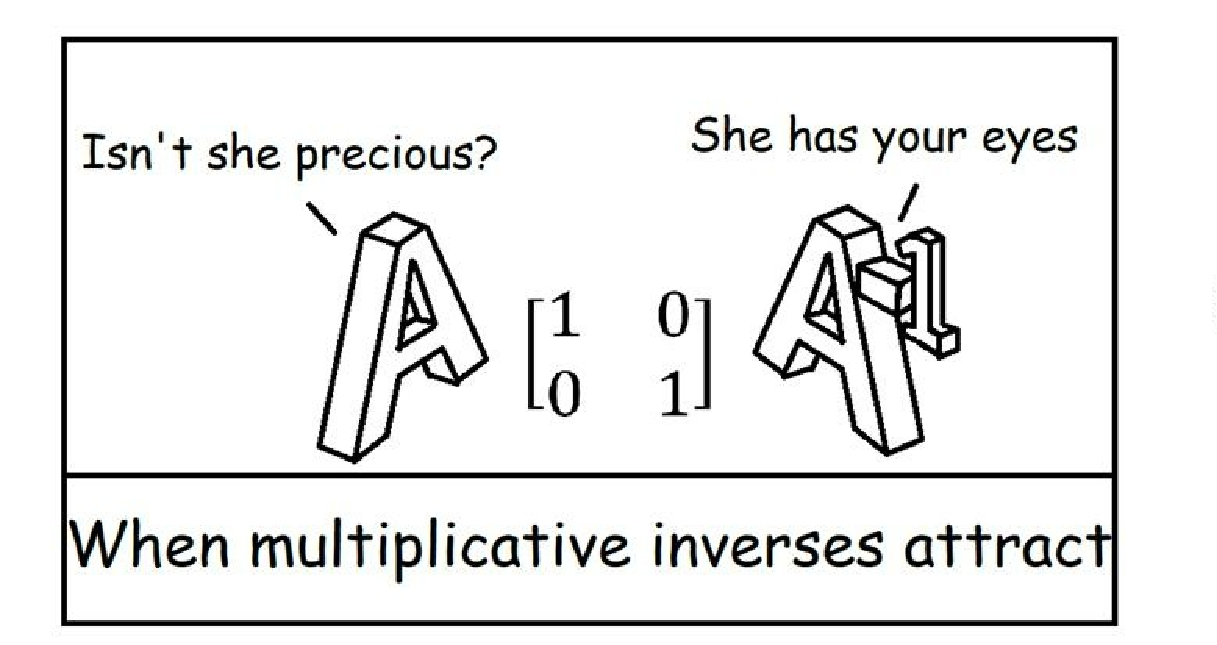
\includegraphics[scale=0.5]{Chapter3/images/attract.pdf}}
%{\vspace{-10 pt}\hfill\footnotesize (Image contributed by Thayne Hansen)}\\

\pagebreak  %The Algebra and Geometry of Matrices
\begin{center} 
\emph{``The thing that scares us the most is when familiar things operate in unfamiliar ways.'' -- Noah Hawley}
\end{center}

\section{Matrix Operations}\label{sec:matrix}
We say that two $m\times n$ matrices $A = \mtx{r}{a_{ij}}$ and $B = \mtx{r}{b_{ij}}$ are \textbf{equal} if $a_{ij} = b_{ij}$ for all $i$ and $j$ (for all $a_{ij}, b_{ij}\in F$). We can \textbf{add} matrices term-wise,  that is, 
\[A + B = \mtx{r}{a_{ij}+b_{ij}}.\] Finally, we can \textbf{multiply} matrices by a \textbf{scalar} term-wise, that is, 
\[cA = \mtx{r}{ca_{ij}}\qquad\text{for all $c\in F$}.\]\vs

%Hailey Checketts
\begin{Exam} Let $A = \mtx{rrr}{3&9&1\\-2&4&6}$, $B = \mtx{rrr}{0&5&6\\3&1&1}$, and $C = \mtx{rr}{2&1\\0&4}$.\\

Then \[A + B = \mtx{rrr}{3+0&9+5&1+6\\-2+3&4+1&6+1} = \mtx{rrr}{3&14&7\\1&5&7}.\] Now, $A+C$ is not possible since the matrices have different sizes.\\

Next, \[2B = 2\mtx{rrr}{0&5&6\\3&1&1} = \mtx{rrr}{0&10&12\\6&2&2},\] and \[A - 2B =  \mtx{rrr}{3&9&1\\-2&4&6} - \mtx{rrr}{0&10&12\\6&2&2} = \mtx{rrr}{3&-1&-11\\-8&2&4}.\qedhere\]
\end{Exam}\vs

Because we can add and scale matrices, we can actually view matrices as vector themselves. Let $F$ be a field. Then $F^{m\times n}$ will denote the set of $m\times n$ matrices with entries from $F$, which is a vector space. This means that addition of matrices and multiplication of scalars follow the eight algebraic properties listed in \defref{def:vectorspace}. When working with matrices, we will let $0$ denote an $m\times n$ matrix with all entries equal to zero. This is called the \textbf{zero matrix}.\\

Let $E_{ij}$ be the matrix whose entry in the $(i,j)$th entry is a one and all other entries are zero. Then $\mathcal{E} = \{E_{1,1}, E_{1,2}, \ldots, E_{1,n}, E_{2,1}, E_{2,2},\ldots, E_{2,n},\ldots, E_{m,1}, E_{m,2}, \ldots, E_{m,n}\}$ forms the \textbf{standard basis} of $F^{m\times n}$. The matrices $E_{i,j}$ are often called the \text{unit matrices}. Using coordinate vectors, we see that $F^{m\times n} \cong F^{mn}$, since $|\mathcal{E}| = mn$.\\

\begin{Def} The \textbf{diagonal entries} in an $m\times n$ matrix $A  = \mtx{r}{a_{ij}}$ are the entries $a_{11}$, $a_{22}$, $a_{33}, \ldots$, that is, the entries $a_{ii}$, and they form the \textbf{main diagonal}.\\

If $A$ is an $n\times n$ matrix, then we say that $A$ is a \textbf{square matrix}.\\

Let $I_n$ denote the $n\times n$ matrix whose entries are $1$'s across the diagonal and $0$'s everywhere else. This matrix is known as the \textbf{identity matrix}.
\end{Def}\vs

\begin{Def} If $A$ is an $m\times n$ matrix and $B$ is an $n\times p$ matrix with column vectors 
\[B = \mtx{rrrr}{\bb b_1 & \bb b_2 & \ldots & \bb b_p},\] then the \textbf{matrix product}
\[AB = A\mtx{rrrr}{\bb b_1 & \bb b_2 & \ldots & \bb b_p} = \mtx{rrrr}{A\bb b_1 & A\bb b_2 & \ldots & A\bb b_p}.\] The matrix $AB$ is a $m\times p$ matrix.\\

If $A$ is an $n\times n$ matrix, then $A^k = \underbrace{A\cdots A}_{k}$. We let $A^0 = I_n$.
\end{Def}\vs

Matrix multiplication can also be defined with the seemingly complicated formula, 
\[AB = \mtx{r}{\dsum_{k=1}^na_{ik}b_{kj}} = \mtx{r}{a_{i1}b_{1j} + a_{i2}b_{2j} + \ldots + a_{in}b_{nj}}\qquad \text{for } A = \mtx{r}{a_{ik}} \text{ and } B= \mtx{r}{b_{kj}},\] which is none other than the ``finger-multiplication" we learned with the matrix-vector product.\\

%Hailey Checketts
\begin{Exam} Compute $AB$ with the given matrices $A = \mtx{rrr}{2&1&-1\\0&4&-2}$ and $B = \mtx{rrr}{9&-5&-3\\3&9&1\\-2&4&6}$.
\[AB = \mtx{rrr}{A\vr{9\\3\\-2} & A\vr{-5\\9\\4} & A\vr{-3\\1\\6}}= \mtx{rrr}{2(9)+1(3)-1(-2) & 2(-5)+1(9)-1(4) & 2(-3)+1(1)-1(6) \\ 0(9)+4(3)-2(-2) & 0(-5)+4(9)-2(4) & 0(-3)+4(1)-2(6)}\]\[  = \mtx{rrr}{18+3+2 & -10+9-4 & -6+1-6 \\ 0+12+4 & 0+36-8 & 0+4-12} = \mtx{rrr}{23&-5&-11\\16&28&-8},\] which is a $2\times 3$ matrix.
\end{Exam}\vs


\begin{Def} If $A$ is a square matrix, say $n\times n$, and if 
\[p(x) = a_0 + a_1x + a_2x^2 + \ldots + a_mx^m\] is a degree $m$ polynomial, then we define the $n\times n$ matrix $p(A)$ to be 
\[p(A) = a_0I_n + a_1A + a_2A^2 + \ldots + a_mA^m.\] An expression of this form is called a \textbf{matrix polynomial} in $A$.
\end{Def}\vs


\begin{Exam} Find $p(A)$ for $p(x) = x^2+3x+2$ and $A=\mtx{rr}{4&2\\0&3}$ over $\Z_5$.
\begin{multline*}
p(A) \equiv A^2+3A+2I \equiv \mtx{rr}{4&2\\0&3}^2 + 3\mtx{rr}{4&2\\0&3} + 2\mtx{rr}{1&0\\0&1}\\
\equiv \mtx{rr}{1&4\\0&4} + \mtx{rr}{2&1\\0&4} + \mtx{rr}{2&0\\0&2} \equiv \mtx{rr}{0 & 0\\0 & 0} \qedhere
\end{multline*}
\end{Exam}\vs

\begin{Def} Let $A = \mtx{r}{a_{ij}}$ be an $m\times n$ matrix. Then the \textbf{transpose} of $A$, denoted $A^\top $, is the $n\times m$ matrix given by $A^\top  = \mtx{r}{a_{ji}}$, that is, the matrix whose columns are formed from the corresponding rows of $A$.
\end{Def}\vs

%Adym Warhurst
\begin{Exam}  Let \[\begin{tikzpicture}
\begin{scope}
\clip (-1.5,0.75) rectangle (1.5,-0.75);
\fill[cyan] (-0.4,0.75) rectangle (0,-0.75);
\fill[magenta] (0.11,0.75) rectangle (0.51,-0.75);
\fill[lime] (0.65,0.75) rectangle (1.05,-0.75);
\path (0,0) node {$A = \mtx{rrr}{1&2&3\\4&5&6}$\text{,}};
\end{scope}
\begin{scope}[shift={(3,0)}]
\clip (-1.5,0.75) rectangle (1.5,-0.75);
\fill[cyan] (-0.4,0.75) rectangle (0,-0.75);
\fill[magenta] (0.11,0.75) rectangle (0.51,-0.75);
\fill[lime] (0.65,0.75) rectangle (1.05,-0.75);
\path (0,0) node {$B = \mtx{rrr}{1&1&1\\3&5&7}$\text{,}};
\end{scope}
\begin{scope}[shift={(6.25,0)}]
\fill[cyan] (0.09,0.75) rectangle (0.69,-0.75);
\fill[magenta] (0.77,0.75) rectangle (1.37,-0.75);
\path (0,0) node {\text{ and } $C = \mtx{rr}{2&-3\\0&1}.$};
\end{scope}
\end{tikzpicture}\] Then 
\[
\begin{tikzpicture}
\fill[cyan] (-0.2,0.9) rectangle (1.07,0.5);
\fill[magenta] (-0.2,0.15) rectangle (1.07,-0.25);
\fill[lime] (-0.2,-0.55) rectangle (1.07,-0.95);
\path (0,0) node {$A^\top  = \mtx{rr}{1&4\\2&5\\3&6}$\text{,}};
\begin{scope}[shift={(3,0)}]
\fill[cyan] (-0.2,0.9) rectangle (1.07,0.5);
\fill[magenta] (-0.2,0.15) rectangle (1.07,-0.25);
\fill[lime] (-0.2,-0.55) rectangle (1.07,-0.95);
\path (0,0) node {$B^\top  = \mtx{rr}{1&3\\1&5\\1&7}$\text{,}};
\end{scope}
\begin{scope}[shift={(6.25,0)}]
\fill[cyan] (0,0.58) rectangle (1.55,0.08);
\fill[magenta] (0,-0.1) rectangle (1.55,-0.7);
\path (0,0) node {$\text{and } C^\top  = \mtx{rr}{2&0\\-3&1}$.};
\end{scope}
\end{tikzpicture}
\qedhere\]
\end{Exam}\vs

In the case of $\C$-matrices, an alternative to transposes is preferred for reasons that will be explained in Chapter 4.\\

\begin{Def} Let $A$ be an $m\times n$ complex matrix. Then we define $A^* = (\overline{A})^\top $, which is called the \textbf{conjugate transpose}. This replaces the role of transposes in complex space.
\end{Def}\vs

When discussing transposes of matrices, whenever the matrices are complex, the conjugate transpose should ALWAYS be used instead of the standard transpose.\\

%Tyler Bayn
\begin{Exam} Let $A = \mtx{ccc}{ 1-2i & 3+5i & 6 \\ -2i & 0 & i}$ and  $B = \mtx{ccc}{2-3i & 0 & 2i \\ -i & 4 & 1+2i \\ 0 & 2-2i & 6}$.\\

 Note that 
\[A^* = \mtx{cc}{1+2i & 2i \\ 3-5i & 0 \\ 6 & -i},\qquad B^* =  \mtx{ccc}{2+3i & i & 0 \\ 0 & 4 & 2+2i \\ -2i & 1-2i & 6}. \qedhere \]
\end{Exam}\vs

\begin{Def} If $A$ is a square matrix, then the \textbf{trace} of $A$, denoted $\tr(A)$, is the sum of the diagonal entries of $A$.
\end{Def}\vs

%Hailey Checketts
\begin{Exam} Let $A = \mtx{rr}{2&0\\1&4}$ and $B = \mtx{rrrr}{9&3&-2&3\\28&9&4&0\\16&1&6&3\\2&5&2&1}$. Then 
\[\tr(A) = 2+4 = \fbox{$6$},\qquad \tr(B) =9+9+6+1 = \fbox{$25$}.\qedhere\]
\end{Exam}\vs

%%%%%%%%%%%%%%%%%%% Exercises %%%%%%%%%%%%%%%%%%%
\startExercises{matrix}

\noindent For Exercises \ref{true:matrixstart}-\ref{true:matrixstop}, determine with the statement is true or false. If false, correct the statement so that it is true.
\begin{enumerate}[!HW!, start=1]
\item\label{true:matrixstart} We say that two $m\times n$ matrices $A=[a_{ij}]$ and $B=[b_{ij}]$ are equal if $a_{ij}=b_{ij}$ for all $i$ and $j$. %Carson Blickenstaff
\item If $A$ is a square matrix, then the trace of $A$ is the sum of the column entries of $A$. %Carson Blickenstaff
\item We can multiply matrices by a scalar term-wise. %Carson Blickenstaff
\item The identity matrix is an $n\times n$ matrix whose entries are $1$'s across the main diagonal and zeros everywhere else. %Carson Blickenstaff
\item If $A$ is an $n\times n$ matrix, then we say that $A$ is a square matrix. %Carson Blickenstaff
\item\label{true:matrixstop} The transpose of a matrix $A$ is a matrix whose columns are formed from the corresponding rows of $A$.\\ %Carson Blickenstaff
\end{enumerate}

\begin{enumerate}[!HW!]
\item Write the matrix $E_{1,3}\in F^{3\times 3}$.
\end{enumerate}

\noindent For Exercises \ref{exer:matrixwhatwrongstart}-\ref{exer:matrixwhatwrongstop}, using the matrices listed below, explain why the operation is not possible.
\[A = \mtx{rr}{2&3\\1&4},\quad B = \mtx{rr}{1&1\\3&6}, \quad C = \mtx{rrr}{2&7&5\\1&5&4},\quad D=\mtx{rrr}{1&6&4\\5&9&2\\9&3&3}.\]
\begin{enumerate}[!HW!]
\begin{multicols}{3}
\item\label{exer:matrixwhatwrongstart} $CA$ %Jacob Kuhn
\item $ABD$%Jacob Kuhn
\item\label{exer:matrixwhatwrongstop} $\tr(C)$ %Jacob Kuhn
\end{multicols}
\end{enumerate}

\noindent For Exercises \ref{exer:matrixcomputerealstart}-\ref{exer:matrixcomputerealstop}, using the matrices listed below, perform the matrix calculation:
\[A = \mtx{rrr}{1&2&3\\4&-3&0\\1&-2&-1},\quad B = \mtx{rrr}{0&5&6\\-5&-5&2\\2&0&-3}, \quad C = \mtx{rrrr}{3&0&-1&2\\1&7&8&-3\\3&3&2&-4},\quad D=\mtx{rrr}{2&3&-2\\-5&0&7\\0&-2&4\\1&2&3}.\]
\begin{enumerate}[!HW!, label=$\spadesuit$ \arabic*., ref=\arabic*]
\begin{multicols}{6}
\item\label{exer:matrixcomputerealstart} $2A+B^\top$\columnbreak %Alexis Borell
\itemspade $4A-3B$ \columnbreak
\itemspade $AC$ \columnbreak
\itemspade $A^\top$ \columnbreak
\itemspade $C^\top$ \columnbreak
\itemspade $D^\top$
\end{multicols}
\begin{multicols}{4}
\itemspade $\tr(A)$
\itemspade $\tr(B)$
\itemspade $DB^\top $
\item\label{exer:matrixcomputerealstop} $A^2 + 2A-5I_3$
\end{multicols}
\end{enumerate}

%NEW
\noindent For Exercises  \ref{exer:matrixcomputeboringstart}-\ref{exer:matrixcomputeboringstop}, using the matrices listed below, perform the matrix calculation over the field $\R$:
\[A = \mtx{rrr}{-1&0&2\\1&3&5},\quad B = \mtx{rrr}{5&1\\2&2\\3&4}, \quad C = \mtx{rrrr}{-2&0\\3&-2}.\]
\begin{enumerate}[!HW!]
\begin{multicols}{4}
\item\label{exer:matrixcomputeboringstart} $2A^\top+B$ 
\item$AB$ 
\item $BC$ 
\item\label{exer:matrixcomputeboringstop} $ABC$ 
\end{multicols}
\end{enumerate}

\noindent For Exercises \ref{exer:matrixcomputecomplexstart}-\ref{exer:matrixcomputecomplexstop}, using the matrices listed below, perform the matrix calculation over the field $\C$:
\[A = \mtx{cc}{1+2i & 1-3i \\ 5 & 1-i },\quad B = \mtx{cc}{0 & 3-4i \\ 3i & 1+i}, \quad C = \mtx{cc}{3&0\\i&2i\\3+i&1+3i},\quad D=\mtx{cccc}{1& 0 & i & 1-2i \\ 5  & 4+i & 0 & -4}.\]
\begin{enumerate}[!HW!, label=$\spadesuit$ \arabic*., ref=\arabic*]
\begin{multicols}{5}
\item\label{exer:matrixcomputecomplexstart} $(1+i)A-3B$\\
\item $CA$
\item $A^*$
\item $C^*$
\item $D^*$
\end{multicols}
\begin{multicols}{4}
\item $\tr(A)$
\item $\tr(B)$
\item $(BD)^*$
\item\label{exer:matrixcomputecomplexstop} $A^2+I_2$
\end{multicols}
\end{enumerate}

\noindent For Exercises \ref{exer:matrixcomputefivestart}-\ref{exer:matrixcomputefivestop}, using the matrices listed below, perform the matrix calculation over the field $\Z_5$:
\[A \equiv \mtx{rrrr}{1&2&3&4\\0&2&2&3\\1&2&2&1\\4&4&3&2},\quad B \equiv \mtx{rrrr}{0&1&1&2\\2&2&3&0\\1&2&3&2\\4&3&4&2}, \quad C \equiv \mtx{rrrr}{3&0&4&2\\1&2&3&2\\3&3&2&1},\quad D\equiv\mtx{rrr}{2&3&3\\0&0&2\\0&3&4\\1&2&3} \pmod 5.\]
\begin{enumerate}[!HW!, label=$\spadesuit$ \arabic*., ref=\arabic*]
\begin{multicols}{5}
\item\label{exer:matrixcomputefivestart} $2A-3B$
\item $CA$
\item $A^\top $ 
\item $C^\top $
\item $D^\top $
\end{multicols}
\begin{multicols}{4}
\item $\tr(A)$
\item $\tr(B)$
\item $D^\top B$
\item\label{exer:matrixcomputefivestop} $A^2+A-I_4$
\end{multicols}
\end{enumerate}

\noindent For Exercises \ref{exer:mtxtracerealstart}-\ref{exer:mtxtracerealstop}, for the matrix $A$ provided, find $\tr(A)$, $A^\top $, and $\tr(A^\top )$.
\begin{enumerate}[!HW!]
\begin{multicols}{4}
\item\label{exer:mtxtracerealstart} $\mtx{rrr}{8&-7&2\\0&-2&4\\3&2&1}$ %Daven Triplett
\item $\mtx{rrrr}{1/8&-7/8&2/5&-12/13\\9/8&-1/2&1/4&1/4\\1&-12/15&2&1/5\\1/4&8/15&-3/8&3/8}$ %Daven Triplett

\mbox{}

\item\label{exer:mtxtracerealstop} \mbox{$\mtx{rrrr}{5&1&6&2\\3&0&3&4\\5&2&1&1\\2&3&0&0}\pmod 7$} %Daven Triplett
\end{multicols}
\end{enumerate}

\noindent For Exercises \ref{exer:mtxtracecomplexstart}-\ref{exer:mtxtracecomplexstop}, for the matrix $A$ provided, find $\tr(A)$, $A^*$, and $\tr(A^*)$.
\begin{enumerate}[!HW!]
\item\label{exer:mtxtracecomplexstart}\label{exer:mtxtracecomplexstop} $A=\mtx{ccc}{1-3i&-5-5i&2+2i\\2-4i&8i&6+i\\-1+2i&3-6i&2+4i}$\\ %Daven Triplett
\end{enumerate}

%%%%%%%%%%%%%%%%%%% Footnotes %%%%%%%%%%%%%%%%%%%
 %\mbox{}\vfill
 \pagebreak%3.1 Matrix Operations

\begin{center} 
\emph{``When you put your hand to the plow, you can't put it down until you get to the end of the row.''\\ -- Alice Paul}
\end{center}

\section{Matrix Properties}\label{sec:rowspace}
We mentioned in the previous section that $F^{m \times n}$, meaning that matrix addition and scalar multiplication satisfy the eight properties listed in \defref{def:vectorspace}. Transposes and traces also follow very nice algebraic properties.\\

\begin{Thm}  Let $A$ and $B$ be matrices with sizes such that the indicated sums and products are defined. Let $c\in F$.
\begin{multicols}{2}
\begin{enumerate}[!THM!, start=1]
\item $(A+B)^\top  = A^\top  + B^\top $\\
\item $(cA)^\top  = cA^\top $\\
\item $(A^\top )^\top  = A$\\
\item $(AB)^\top  = B^\top A^\top $\\
\end{enumerate}
\end{multicols}
\end{Thm}\vspace{-0.15 in}

We see by the first two properties that transposition is a linear transformation $\mbox{}^\top  : F^{m\times n} \to F^{n\times m}$. Note the last property states that the transpose of a product of matrices equals the product of their transposes in the reverse order! This is called the \emph{Shoe-Sock Principle}\footnotemark[2]. As we will see momentarily, this order matters a lot.\\ 

\begin{Thm}  Let $A$ and $B$ be $n\times n$ matrices. Let $c\in F$.
\begin{multicols}{2}
\begin{enumerate}[!THM!, start=1]
\item $\tr(A+B) = \tr(A) + \tr(B)$\\
\item $\tr(cA) = c\tr(A)$\\
\item $\tr(A^\top ) = \tr(A)$\\
\item $\tr(AB) = \tr(BA)$\\
\end{enumerate}
\end{multicols}
\end{Thm}\vspace{-0.15 in}

We see by the first two properties that the trace is a linear transformation $\tr : F^{m\times n} \to F$. It should be mentioned that the last property does NOT say that $\tr(AB) = \tr(A)\tr(B)$. This is, in fact, very false. Also, this property does NOT say that $AB=BA$ only that $\tr(AB) = \tr(BA)$. As hinted to already, we will soon see that $AB \neq BA$, in general. \\ 

Unfortunately, matrix multiplication is not as well behaved as multiplication of real numbers which we are used to. Many of the typical algebraic properties do hold.\\

\begin{Thm} Let $A$, $B$, and $C$ be matrices with sizes such that the indicated sums and products are defined. Let $c\in F$.
\begin{multicols}{2}
\begin{enumerate}[!THM!, start=1]
\item $A(BC) = (AB)C$\\
\item $A(B+C) = AB + AC$\\
\item $(A+B)C = AC + BC$\\
\item $c(AB) = (cA)B = A(cB)$\\
\item Let $A$ be an $m\times n$ matrix. Then \[I_mA = A = AI_n.\] \mbox{}
\end{enumerate}
\end{multicols}
\end{Thm}\vspace{-0.15 in}

Please be aware that certain multiplicative properties in the previous list are omitted. This is quite intentional because many algebraic properties that we take for granted with real multiplication do NOT hold for matrix multiplication.\\

\begin{Thm}\label{thm:cantmultiply} Let $A$, $B$, and $C$ be matrices with sizes such that the indicated sums and products are defined.
\begin{enumerate}[!THM!, start=1]
\item\label{item:cantmultiplycommute} You CANNOT assume that $AB = BA$\\
\item You CANNOT assume that if $AB=AC$, then $B = C$\\
\item You CANNOT assume that if $AB = 0$, then $A =0$ or $B=0$.
\end{enumerate}
\end{Thm}

\begin{Exam} Let $A = \mtx{rr}{1 & 2\\-1&3}$ and $B = \mtx{rr}{0&-3\\1&1}$. Then 
\[AB = \mtx{rr}{1 & 2\\-1&3}\mtx{rr}{0&-3\\1&1} = \mtx{rr}{2&-1\\3&6}\quad\text{and}\quad BA = \mtx{rr}{0&-3\\1&1}\mtx{rr}{1 & 2\\-1&3} = \mtx{rr}{3&-9\\0&5}.\] Therefore, $AB\neq BA$.
\end{Exam}\vs

\begin{Exam} Let $A = \mtx{rr}{0&2\\0&-1}$, $B = \mtx{rr}{1&2\\3&4}$, and $C = \mtx{rr}{5&6\\3&4}$. Then 
\[AB = \mtx{rr}{0(1)+2(3)& 0(2)+2(4)\\ 0(1)-(3)& 0(2)-(4)} = \mtx{rr}{6&8\\-3&-4} \quad\text{and}\quad AC = \mtx{rr}{0(5)+2(3)& 0(6)+2(4)\\ 0(5)-(3)& 0(6)-(4)} = \mtx{rr}{6&8\\-3&-4}.\] Therefore, $AB=AC$ but $B\neq C$. In other words, we cannot divide both sides by $A$.
\end{Exam}\vs

\begin{Exam} Let $A = \mtx{rr}{0&2\\0&-1}$ and $B = \mtx{rr}{4&2\\0&0}$. Then
\[AB = \mtx{rr}{0(4)+2(0)& 0(2)+2(0)\\ 0(4)-(0)& 0(2)-(0)} = \mtx{rr}{0&0\\0&0},\] which is the zero matrix. Therefore, $AB=0$ but $A\neq 0$ not $B\neq C$. In other words, the zero product property does NOT hold for matrices.
\end{Exam}\vs

\begin{Def} Let $A$ be an $m\times n$ matrix. Define the \textbf{row space} of $A$, denoted $\row A$, as the column space of $A^\top $, that is, $\row A = \col A^\top $. \\

The dimension of $\row A$ is called the \textbf{corank}, denoted $\corank A = p$, where $p$ is the number of pivots in $A$. 
\end{Def}\vs

Note that the corank is not really a new quantity. Note that $\corank(A) = \dim(\row A) = \text{the number of pivot positions} = \rank A = \dim(\col A)$.\\

For another way to describe the row space of $A$, note that each row of $A$ contains $n$ entries and can be identified with a vector in $F^n$. Then $\row A$ is the span of the rows of $A$ under this identification.\\

\begin{Thm}\label{thm:rowspaceequivalence} Two matrices $A$ and $B$ are row equivalent if and only if $\row A = \row B$.
\end{Thm}\vs
%\begin{proof} We will show that if $A\sim B$, that is, if $A$ and $B$ are row equivalent, then $\row A = \row B$. Let $\{\bb r_1, \ldots, \bb r_m\}$ be the rows of $A$. Certainly, interchange would not change the row space since 
%\[\Span\{\bb r_1, \ldots, \bb r_i, \ldots, \bb r_j,\ldots, \bb r_m\} = \Span\{\bb r_1, \ldots, \bb r_j, \ldots, \bb r_i,\ldots, \bb r_m\}.\] Additionally, scaling by a nonzero value $c$ does not affect the span of the rows since 
%\[c\bb r_i \in \Span\{\bb r_1, \ldots, \bb r_i, \ldots, \bb r_m\}\qquad\text{and}\qquad \bb r_i - \frac{1}{c}(c\bb r_i) \in \Span\{\bb r_1, \ldots, c\bb r_i, \ldots,  \bb r_m\}.\] Finally, replacement also does not change the row space because 
%\[\bb r_j + c\bb r_i \in \Span\{\bb r_1, \ldots, \bb r_i, \ldots, \bb r_j,\ldots, \bb r_m\}\qquad\text{and}\qquad \bb r_j = (\bb r_j +c\bb r_i) - c\bb r_i \in \Span\{\bb r_1, \ldots, \bb r_i, \ldots, \bb r_j+c\bb r_i,\ldots, \bb r_m\}.\] Since no row operation changes the row space, $\row A = \row B$ for all $A\sim B$. The other direction is handled similarly.
%\end{proof}\vs

\begin{Thm}\label{thm:rowspaceequivalencerref} If $U$ is an echelon form of the matrix $A$, then nonzero rows of $U$ form a basis for the row space of $A$.
\end{Thm}\vs
%\begin{proof}
% It was shown previously that $\row(A) = \row(U)$ since $A$ and $U$ are row equivalent. Thus, a basis for $\row(U)$ is a basis for $r\row(A)$. If $U$ is in echelon form, then no nonzero row can be written as a linear combination of the other rows (otherwise we could have zeroed out that row). Thus, the nonzero rows give a basis.
%\end{proof}\vs

Much like the column space of $A$, the pivot rows of $A$ also form a basis of $\row(A)$. But unlike the column space, the pivot rows of $U$ form a basis of $\row(A)$. This is not true for the column space, that is, the pivot columns of $U$ do NOT form a basis for $\col(A)$. This is because row equivalent matrices need not have the same column space. Only the row space is guaranteed to be equal.\\

%Walt Williams
\begin{Exam} Let $A = \mtx{rrrrr}{1 & 3 & 2 & 4 & 2 \\
 2 & 6 & 4 & 8 & 4 \\
 3 & 2 & 5 & 2 & 1 \\
 4 & 2 & 5 & 1 & 0 \\}$. Compute a basis for $\row A$, $\col A$, and $\nul A$.\\

Since \[A = \mtx{rrrrr}{1 & 3 & 2 & 4 & 2 \\
 2 & 6 & 4 & 8 & 4 \\
 3 & 2 & 5 & 2 & 1 \\
 4 & 2 & 5 & 1 & 0 \\} \sim \mtx{rrrrr}{ 1 & 0 & 0 & -1 & -1 \\
 0 & 1 & 0 & 15/11 & 7/11 \\
 0 & 0 & 1 & 5/11 & 6/11 \\ 
 0 & 0 & 0 & 0 & 0 \\}.\] Therefore, \[\{(1,0,0,-1,-1), (0,1,0,15/11,7/11), (0,0,1,5/11,6/11)\}\] is a basis for $\row A$. Hence, $\corank(A)=3$. If a basis without fractions is desired, those vectors can be scaled by $11$ without adjusting the span or the linear independence. Thus,  \[\{(1,0,0,-1,-1), (0,11,0,15,7), (0,0,11,5,6)\}\] is another basis of $\row A$.
 \begin{multicols}{2}
 We also see that \[\left\{\vr{1\\2\\3\\4}, \vr{3\\6\\2\\2}, \vr{2\\4\\5\\5}\right\}\] is a basis for $\col A$. Hence, $\rank(A)=3$. \columnbreak
 
 Likewise, \[\left\{\vr{11\\-15\\-5\\1\\0}, \vr{11\\-7\\-6\\0\\1}\right\}\]  is a basis for $\nul A$. Hence, $\nullity(A)=2$. \hfill$\qedhere$
 \end{multicols}
\end{Exam}\vs

Alternatively, one could find a basis for $\row A$ by finding a basis for $\col A^\top $ as we did before. This would, in fact, provide a basis consisting of actual rows of $A$. The method above has the advantage (other than providing simpler vectors) than we can find all these bases of the fundamental spaces of $A$ simultaneously. 

%%%%%%%%%%%%%%%%%%% Exercises %%%%%%%%%%%%%%%%%%%
\startExercises{rowspace}

\begin{enumerate}[!HW!, start=1]
\item Rewrite the eight axioms of a vector space, listed in \defref{def:vectorspace}, as properties of $m\times n$ matrices. \\

\item Verify \thmref{thm:cantmultiply} \ref{item:cantmultiplycommute} using $A=\mtx{rrr}{3&2&1\\1&5&0\\4&1&2}$, $B=\mtx{rrr}{1&3&2\\0&1&4\\2&1&7}$. %Candace Fehr
\end{enumerate}

\noindent For Exercises \ref{exer:rowspacerealstart}-\ref{exer:rowspacerealstop}, for the matrix $A$ provided, find a basis for $\row(A)$ and compute $\corank(A)$. Answers may vary.
\begin{enumerate}[!HW!, label=$\spadesuit$ \arabic*., ref=\arabic*]
\begin{multicols}{2}
\item\label{exer:rowspacerealstart} $\mtx{rrrrr}{8&-3&-13&15&17\\-2&1&3&-3&-3}$ 
\item $\mtx{rrrr}{-1&2&1&0\\7&-14&-7&-8\\-3&6&3&2}$ 
\end{multicols}
\begin{multicols}{2}
\itemspade $\mtx{rrrrrr}{1&0&0&1&1&1\\0&1&0&1&1&0\\0&0&1&1&0&1} \pmod 2$ 
\itemspade $\mtx{rrrr}{2&1&1&1\\4&2&0&3\\2&1&3&0\\0&0&1&2} \pmod 5$
\end{multicols}
\item\label{exer:rowspacerealstop} $\mtx{cccccc}{1+2i&2-i&-1&0&1+i&-3+3i\\2+4i&4-2i&1+4i&-2&2+5i&-2+10i\\3-i&-1-3i&2&i&3-i&6+3i}$ 
\end{enumerate}

\noindent For Exercises \ref{exer:rowcolumnstart}-\ref{exer:rowcolumnstop}, let $A$ be the matrix provided on the left. The second matrix is row equivalent to $A$. Find a basis for $\col(A)$ and $\row(A)$ and compute $\rank(A)$ and $\corank(A)$.
\begin{enumerate}[!HW!]
\item\label{exer:rowcolumnstart}\label{exer:rowcolumnstop} $\mtx{rrrrrr}{
1&1&-3&7&9&-9\\
1&2&-4&10&13&-12\\
1&-1&-1&1&1&-3\\
1&-3&1&5&7&3\\
1&-2&0&0&-5&4} 
\sim \mtx{rrrrrr}{
1&1&-3&7&9&-9\\
0&1&-4&3&4&-3\\
0&0&0&1&-1&2\\
0&0&0&0&0&0\\
0&0&0&0&0&0}$ %Noah Swenson
\end{enumerate}

\begin{enumerate}[!HW!]
\item Show that $\R^{2\times 2}$ with respect to matrix addition and matrix multiplication is NOT a field. 

\item Show that if $F$ is any field and $n$ a positive integer, then $F^{n\times n}$ is a field if and only if $n=1$. 
\end{enumerate}

%%%%%%%%%%%%%%%%%%% Footnotes %%%%%%%%%%%%%%%%%%%
 \mbox{}\vfill
 \footnotetext[2]{\emph{In the morning you put your socks on then your shoes. In the evening, you take your shoes off then your socks.}}
 \pagebreak%3.2 Matrix Properties
\begin{center} 
\emph{``My happiness grows in direct proportion to my acceptance, and in inverse proportion to my expectations.'' -- Michael J. Fox}
\end{center}

\section{Matrix Inverses}\label{sec:nonsingular}
When can we divide by a matrix? Does it even make sense to talk about matrix division? It depends on the matrix.\\

\begin{Def} An $n\times n$ matrix $A$ is  \textbf{nonsingular} (or \textbf{invertible}) if there exists an $n\times n$ matrix $B$ such that 
\[AB = BA = I_n.\] In this case, $B$ is called an \textbf{inverse} of $A$. If $A$ is not nonsingular, then it is \textbf{singular}.
\end{Def}\vs

\begin{Exam} Let $A = \mtx{rr}{2&3\\3&5}$ and $C = \mtx{rr}{5&-3\\-3&2}$. Then 
\[AC = \mtx{rr}{2&3\\3&5}\mtx{rr}{5&-3\\-3&2} = \mtx{rr}{1&0\\0&1}\] and \[CA = \mtx{rr}{5&-3\\-3&2}\mtx{rr}{2&3\\3&5} = \mtx{rr}{1&0\\0&1}.\]
Thus, $A$ is invertible with inverse $C$.
\end{Exam}\vs

We should mention that inverses are unique. Suppose that $A$ is invertible with inverses $B$ and $C$. Thus, 
\[B = BI_n = B(AC) = (BA)C = I_nC = C.\] We will denote the inverse of $A$ as $A^{-1}$. Therefore, 
\[AA^{-1} = A^{-1}A = I_n.\]\vs

\begin{Thm}\label{thm:inverseDet} Let $A = \mtx{rr}{a&b\\c&d}$. If $\det(A) := ad-bc\footnotemark[2]\neq 0$, then $A$ is nonsingular with inverse 
\[A^{-1} = \dfrac{1}{ad-bc}\mtx{rr}{d&-b\\-c&a}.\] If $ad-bc=0$, then $A$ is singular.
\end{Thm}


\begin{Exam} Find the inverse of $A = \mtx{rr}{1&2\\3&4}$, if it exists.\\

Since $\det(A) = 1(4)-(2)3 = 4-6 = -2$, $A$ is nonsingular, that is, it has an inverse, which is
\[A^{-1} = -\dfrac{1}{2}\mtx{rr}{4 &-2\\ -3 & 1} = \mtx{rr}{-2 & 1 \\ 3/2 & -1/2}. \qedhere\] 
\end{Exam}\vs

%Jaren Frandsen
\begin{Exam} Find the inverse of $A = \mtx{rr}{9&3\\6&2}$, if it exists.

Since $\det(A)=9(2)-3(6) = 18-18=0$, $A$ has no inverse, that is, $A$ is a singular matrix.
\end{Exam}

For a nonsingular matrix $A$, the equation $A\bb x = \bb b$ has a unique solution for all $\bb b \in F^n$ of the form $\bb x = A^{-1}\bb b$.\\

\begin{Exam} Solve the system of equations 
\[\left\{\begin{alignedat}{100}
&&x_1\ &+\ &2x_2\ &=\ &5&\\
&&3x_1\ &+\ &4x_2\ &=\ &6&.
\end{alignedat}\right.\]

We seek to solve the matrix equation $A\bb x = \bb b$, where $\bb b = \vr{5\\6}$ and $A$ is the matrix from the previous equation. Thus, 
\[A^{-1}(A\bb x) = A^{-1}\bb b \Rightarrow \bb x = A^{-1}\bb b = \mtx{rr}{-2 & 1 \\ 3/2 & -1/2}\vr{5\\6} = \mtx{c}{-4\\9/2}.\qedhere\]
\end{Exam}\vs

\begin{Thm}\label{thm:inverseProps} Let $A$ and $B$ be $n\times n$ invertible matrices, let $m$ be a positive integer, and $r$ is a nonzero real number. Then $A^{-1}$, $AB$, $A^\top $, $A^m$, and $rA$ are also invertible with:\vspace{-0.1 in}
\begin{enumerate}[!THM!, start=1]
\begin{multicols}{3}
\item $(A^{-1})^{-1} = A$\\

\item $(AB)^{-1} = B^{-1}A^{-1}$\footnotemark[8]\\

\item $(A^\top )^{-1} = (A^{-1})^\top $\\
\end{multicols}\vspace{-25 pt}
\begin{multicols}{2}
\item $(A^m)^{-1} = (A^{-1})^m := A^{-m}$\\

\item $(kA)^{-1} = \dfrac{1}{k}A^{-1}$.\\
\end{multicols}
\end{enumerate}
\end{Thm}

\begin{Cor}\label{cor:inverseProps} If $A$ is invertible, then $AA^\top $ and $A^\top A$ are likewise invertible.\end{Cor}\vs

\begin{Exam} Inverse matrices allow us to solve matrix equations when otherwise we may have used division. For example, solve the equation $(AX^{-1})^{-1}+B = C$, assuming all matrices are $n\times n$ and nonsingular (when necessary).\\

We begin by adding $-B$ to both sides of the equation. This gives $(AX^{-1})^{-1} = C-B$. Using the Shoe-Sock Principle, we see that the left-hand side of the equation becomes $(X^{-1})^{-1}A^{-1} = XA^{-1} = C-B$. Finally, if we multiply the equation on both sides by $A$ on the RIGHT side, we get
\begin{eqnarray*}
(XA^{-1})A &=& (C-B)A\\
XA^{-1}A) &=& CA-BA\\
XI_n &=& CA-BA\\
X&=& CA-BA
\end{eqnarray*} The side on which we are multiplying matters. Had we multiplied $A$ on the left, we would have got $AXA^{-1}$ which is not necessarily $X$. Do NOT assume matrices commute. Therefore, $X=\fbox{$CA-BA$}$.
\end{Exam}\vs

\begin{Thm}[The Nonsingular Matrix Theorem] \label{thm:nonsingular} Let $A$ be a square $n\times n$ matrix. Then the following statements are equivalent:
\begin{enumerate}[!THM!, start=1]
\begin{multicols}{2}
\item $A$ is a nonsingular matrix.\\
\item $A$ is an invertible matrix, that is, $A$ has a matrix inverse $A^{-1}$.\\
\item\label{leftinverse} There is an $n\times n$ matrix $C$ such that $CA = I_n$.\\
\item\label{rightinverse} There is an $n\times n$ matrix $C$ such that $AC = I_n$.\\
\item\label{item:nonsingularthmhomo} The equation $A\bb x =\bb 0$ has only the trivial solution.\\
\item\label{item:nonsingularthmnullity} The linear system $A\bb x = \bb b$ has no free variables for each $\bb b\in F^n$.\\
\item The equation $A\bb x = \bb b$ is consistent for each $\bb b\in F^n$.\\
\item $A^\top $ is an invertible matrix.\\
\item $A$ is row equivalent to $I_n$.\\
\item $A$ has $n$ pivot position.\\
\item The rank of $A$ is $n$.\\
\item The columns of $A$ span $F^n$.\\
\item The columns of $A$ form a linearly independent set.\\
\item The columns of $A$ form a basis for $F^n$.\\
\item The rows of $A$ span $F^n$.\\
\item The rows of $A$ form a linearly independent set.\\
\item The rows of $A$ form a basis for $F^n$.\\
\item The linear transformation $\bb x\mapsto A\bb x$ is injective (one-to-one).\\
\item The linear transformation $\bb x \mapsto A\bb x$ is surjective (onto).\\
\item The linear transformation $\bb x \mapsto A\bb x$ is bijective (one-to-one and onto).\\
\end{multicols}
\end{enumerate}
\end{Thm}
%\begin{proof}
%Through varies theorem, corollaries, and comments already proven, we see that (a)--(i) are all equivalent. We have not yet discussed how (j) and (k) are equivalent to the rest. We will first show that (a) and (j) are equivalent.\\
%
% Clearly, (a) implies (j). So, it suffices to show that (j) implies (a). Suppose that (j) holds, that is, there exists some matrix $C$ such that $CA = I_n$. Since (a) is equivalent to (g), we need only show that the only solution to $A\bb x = \bb 0$ is trivial. Suppose that $\bb{x_0}$ is any solution to $A\bb x = \bb 0$, that is, $A\bb{x_0} = \bb 0$. Multiplying on the left by $C$ then gives 
%\begin{eqnarray*}
%C( A\bb{x_0}) &=& C\bb 0\\
%(CA)\bb{x_0} &=& \bb 0\\
%\bb{x_0} &=& \bb 0,\quad\text{by (j).}
%\end{eqnarray*} Therefore, there is only the trivial solution to the homogeneous system, which implies (g).\\
%
%We next show that (a) is equivalent to (k). Like before, clearly (a) implies (k). To see that (k) implies (a), suppose that (k) holds, that is, 
%$AC = I_n$ for some matrix $C$. But by (j), this means that $C$ is invertible, because there exists some matrix $A$ such that $AC = I_n$. In particular, it must be that $A = C^{-1}$ by the uniqueness of the inverse of $C$. But $A = (A^{-1})^{-1}$, which shows that $A$ is invertible, implying (a).
%\end{proof}\vs

%We have already proven many of these equivalences. The remaining ones will be proven in the next lecture. More equivalences will be added in to this list in forthcoming lectures.\\

\begin{Cor}\label{cor:nonsingularthm} Let $A$ and $B$ be $n\times n$ matrices. If $AB$ is invertible, then $A$ and $B$ are likewise invertible.\\
\end{Cor}


\begin{Exam} Determine whether the following matrices are ``nonsingular,'' ``singular,'' or not enough information.
\begin{enumerate}
\item Suppose that $A$ is a $3\times 3$ matrix over $\C$ such that $\nullity(A)=0$.\\

By part \ref{item:nonsingularthmnullity} of the Nonsingular Matrix Theorem, we see that $A$ is nonsingular since the nullity is equal to the number of free variables in the linear system $A\bb x=\bb b$.\\

\item Suppose $A$ is a $5\times 5$ matrix over $\Z_2$. Furthermore, suppose that the equation $A\bb x = \bb 0$ has 8 solutions.\\

By part \ref{item:nonsingularthmhomo} of the Nonsingular Matrix Theorem, we see that $A$ is singular since the homogeneous equation $A\bb x=\bb0$ has nontrivial solutions.\\

\item Suppose $A$ is a $2\times 2$ matrix such that 
\[A\vr{1\\2} = \vr{1\\2}.\] 
We do not have enough information to decide if $A$ is nonsingular or not. On the one hand, the identity matrix $\mtx{cc}{1&0\\0&1}$ satisfies this condition and is nonsingular. On the other hand, $\mtx{rr}{1&0\\2&0}$ also satisfies this condition but is singular.
\end{enumerate}
\end{Exam}\vs


%%%%%%%%%%%%%%%%%% Exercises %%%%%%%%%%%%%%%%%%%
\startExercises{nonsingular}

\noindent For Exercises \ref{exer:twobytwoinverserealstart}-\ref{exer:twobytwoinverserealstop}, compute the inverse matrix of the given matrix using \thmref{thm:inverseDet}. Verify your inverse.  
\begin{enumerate}[!HW!, start]
\begin{multicols}{4}
\item\label{exer:twobytwoinverserealstart} $\mtx{rr}{2&5\\1&3}$ %Riley Drishinski
\item $\mtx{rr}{1&2\\3&4}$ %Riley Drishinski
\item $\mtx{rr}{9&-4\\-7&5}$ %Cyrus Kaveh
\itemspade $\mtx{rr}{2&5\\1&3}$
\end{multicols}
\begin{multicols}{4}
\itemspade $\mtx{rr}{2&5\\3&7}$
\itemspade $\mtx{rr}{4&3\\-2&1}$
\itemspade \mbox{$\mtx{rr}{3&2\\4&2} \pmod5$}
\itemspade \mbox{$\mtx{rr}{10&2\\5&3} \pmod{11}$}
\end{multicols}
\end{enumerate}
\begin{enumerate}[!HW!,label=$\spadesuit$ \arabic*., ref=\arabic*]
\begin{multicols}{4}
\item\label{exer:twobytwoinverserealstop} $ \mtx{cc}{1&1+i\\-i&2}$
\end{multicols}
\end{enumerate}

\noindent For Exercises \ref{exer:solveinversestart}-\ref{exer:solveinversestop}, solve linear system $A\bb x = \bb b$ using the matrix inverse. 
\begin{enumerate}[!HW!, label=$\spadesuit$ \arabic*., ref=\arabic*]
\item\label{exer:solveinversestart} $A = \mtx{rrr}{1&2&3\\-1&-1&1\\2&1&-5}$, $\bb b = \vr{0\\3\\-2}$, $A^{-1} = \mtx{rrr}{4&13&5\\-3&-11&-4\\1&3&1}$
\itemspade $A = \mtx{rrrr}{4&26&31&-15\\-3&-21&-25&12\\1&7&8&-4\\0&-1&-1&1}$, $\bb b = \vr{1\\2\\3\\4}$, $A^{-1} = \mtx{rrrr}{3&4&1&1\\-1&0&4&1\\0&-1&-3&0\\-1&-1&1&2}$
\item \label{exer:solveinversestop} $A \equiv \mtx{rrr}{1&0&1\\2&0&1\\1&2&0}$, $\bb b \equiv \vr{1\\1\\2}$, $A^{-1} \equiv \mtx{rrr}{2&1&0\\2&1&2\\2&2&0}\pmod 3$ 
\end{enumerate}

\noindent For Exercises \ref{exer:nonsingularmatrixthmstart}-\ref{exer:nonsingularmatrixthmstop}, determine whether the following matrices are ``nonsingular,'' ``singular,'' or not enough information. Explain your reasoning.
\begin{enumerate}[!HW!, label=$\spadesuit$ \arabic*., ref=\arabic*]
\begin{multicols}{3}
\item\label{exer:nonsingularmatrixthmstart} $A$ is a  $4\times 4$ matrix with $\rank(A)=4$.\columnbreak
\itemspade $A$ is a  $5\times 4$ matrix with $\rank(A)=4$.\columnbreak
\itemspade $A$ is a  $3\times 3$ matrix such that every vector in $F^3$ can be expressed as $A\bb x$, for some vector $\bb x\in F^3$. 
\end{multicols}\vspace{-15 pt}
\begin{multicols}{3}
\itemspade $A$ is a $5\times 5$ matrix with a two rows of zeros in it row-reduced echelon form.
\itemspade $A$ is a $3\times 3$ matrix in row-reduced echelon form.
\itemspade $A$ is a $3\times 3$ matrix in row-reduced echelon form and a pivot in each column.
\end{multicols}\vspace{-15 pt}
\begin{multicols}{3}
\itemspade $A$ is a $2\times 2$ matrix such that $A\bb x=A\bb y$ for two distinct vectors $\bb x, \bb y\in F^2$.
\itemspade $A$ is row equivalent to a singular matrix.
\item \label{exer:nonsingularmatrixthmstop} $A$ is a $3\times 3$ matrix with columns vectors $\bb a_1$, $\bb a_2$, $\bb a_3$ such that $\bb a_1 - 2\bb a_2 = \bb a_3$.
\end{multicols}
\end{enumerate}

\noindent For Exercises \ref{exer:matrixsolveeqnstart}-\ref{exer:matrixsolveeqnstop}, solve matrix equations for the matrix $X$ using matrix properties. You may assume all matrices are $n\times n$ and nonsingular. Be cautious! The order of multiplication matters!
\begin{enumerate}[!HW!]
\begin{multicols}{3}
\item\label{exer:matrixsolveeqnstart} $(BAX)^{-1} = C$  %Jaden Torgerson
\itemspade $AX+B=0$ 
\itemspade $A^{-1}(AX+C) = BA$
\end{multicols}
\begin{multicols}{3}
\itemspade $(XA)^{-1}B = C$
\itemspade $B(A+X)^{-1} = C$
\item\label{exer:matrixsolveeqnstop} $(DX-B)(CA)^{-1}=E$ %Jaden Torgerson
\end{multicols}
\end{enumerate}

\begin{enumerate}[!HW!]
\item Prove \corref{cor:inverseProps}.

\item Prove \thmref{cor:nonsingularthm}.

% \item Suppose that $A$ is an  $n\times n$ matrix and let $T : F^n \to F^n$ be the linear transformation $T(\bb x) = A\bb x$. Prove that $T$ is invertible if and only if $A$ is nonsingular. 
% \begin{proof}
% First, suppose that $A$ is nonsingular. Suppose that $A\bb x = A\bb y$. Then $A^{-1}A\bb x = A^{-1}A\bb y \Rightarrow \bb x = \bb y$. Thus, $T$ is injective. Next, suppose that $\bb b \in F^n$. Let $\bb x = A^{-1}\bb b$. Then $A\bb x = A(A^{-1}\bb b) = \bb b$. Thus, $T$ is surjective. Therefore, $T$ is bijective.\\

% Suppose next that $T$ is bijective. Then there exists an inverse linear transformation $S : F^n \to F^n$ such that $S\circ T = T\circ S = \Id$, the identity function. Let $B$ be the standard matrix of $S$. Then $BA = AB = I_n$. Therefore, $B = A^{-1}$.
% \end{proof}
\end{enumerate}

%%%%%%%%%%%%%%%%%%% Footnotes %%%%%%%%%%%%%%%%%%%
 \mbox{}\vfill
 \footnotetext[2]{The value $\det(A) = ad-bc$ is called the \textbf{determinant} of $A$. We will learn more about determinants in Chapter 5.}
 \footnotetext[8]{To remember this formula, think of the following proverb:
\begin{center}
\emph{Put Your Socks On, Then Your Shoes\\ Take Your Shoes Off, Then Your Socks}
\end{center}}
\pagebreak%3.3 Matrix Inverses
\begin{center} 
\emph{``The opposite of love is not hate, it's indifference.'' -- Elie Wiesel}
\end{center}

\section{Elementary Matrices}\label{sec:elementary}
\begin{Def} An \textbf{elementary matrix} is a matrix obtained by performing a single row operation on the identity matrix.
\end{Def}\vs

Since there are three types of row operations, there are three types of elementary matrices. Each elementary matrix is nonsingular, whose inverse is the elementary matrix corresponding to the inverse row operation.\\
\begin{enumerate}[!LIST!, start=1]
\item (Replacement) If you replace Row $i$ with Row $i$ + $c$Row $j$ in the identity matrix, then the resulting elementary matrix will have 1's across the main diagonal and 0's everywhere else except in the position $(i,j)$ which will be $c$.\vspace{-0.1 in}
\begin{multicols}{2} For example, the matrix $E_1$, depicted below, corresponds to the row operation\\ ``replace Row 3 with Row 3 - 2Row 1.''\columnbreak

Likewise, the matrix $E_1^{-1}$ is the matrix which corresponds to the inverse row operation\\ ``replace Row 3 with Row 3 + 2Row 1.''
\end{multicols}\vspace{-0.45 in}
\begin{multicols}{2}
\[E_1 = \mtx{rrr}{1&0&0\\0&1&0\\-2&0&1}\]\columnbreak
\mbox{}\\
\[E_1^{-1} = \mtx{rrr}{1&0&0\\0&1&0\\2&0&1}\] 
\mbox{}
\end{multicols}


\item (Interchange) If you interchange Row $i$ with Row $j$ in the identity matrix, then the resulting elementary matrix will be like the identity matrix except the $i$th and $j$th rows are interchanged. \vspace{-0.1 in}
\begin{multicols}{2}
For example, the matrix $E_2$ corresponds to the row operation ``interchange Rows 2 and 3.''\columnbreak

The inverse of $E_2$ is itself! It is also true that $E_2$ is equal to its own transpose.
\end{multicols}\vspace{-0.45 in}
\begin{multicols}{2}
\[E_2 = \mtx{rrr}{1&0&0\\0&0&1\\0&1&0}\]  \columnbreak
\mbox{}\\
\[(E_2)^{-1} = E_2 = (E_2)^\top .\]
\end{multicols} 

\item (Scaling) If you scale Row $i$ by $c$ in the identity matrix, then the resulting elementary matrix has 0's in all off-diagonal entries and 1's in the main diagonal entries except $(i,i)$ which is $c$.\vspace{-0.1 in}
\begin{multicols}{2}
For example, the matrix $E_3$ corresponds to the row operation ``scale Row 2 by 7.''\columnbreak

The inverse of $E_3$ corresponds to the row operation ``scale Row 3 by 1/5.''
\end{multicols}\vspace{-0.45 in}
\begin{multicols}{2}
\[E_3 = \mtx{rrr}{1&0&0\\0&7&0\\0&0&1}\]  \columnbreak
\vfill
\[(E_3)^{-1} = \mtx{rrr}{1&0&0\\0&\frac{1}{7}&0\\0&0&1}.\]
\mbox{}
\end{multicols}
\end{enumerate}\vs

\begin{Exam} Let $A = \mtx{rrr}{a&b&c\\d&e&f\\g&h&i}$.  Using the elementary matrices $E_1, E_2,$ and $E_3$ from above, compute $E_1A, E_2A,$ and $E_3A$.
%\begin{eqnarray*}
\[E_1A =  \mtx{rrr}{1&0&0\\0&1&0\\-2&0&1} \mtx{rrr}{a&b&c\\d&e&f\\g&h&i} =  \mtx{ccc}{a&b&c\\d&e&f\\g-2a&h-2b&i-2c}, \]
\[E_2A = \mtx{rrr}{1&0&0\\0&0&1\\0&1&0}\mtx{rrr}{a&b&c\\d&e&f\\g&h&i} = \mtx{rrr}{a&b&c\\g&h&i\\d&e&f}, \quad E_3A = \mtx{rrr}{1&0&0\\0&7&0\\0&0&1}\mtx{rrr}{a&b&c\\d&e&f\\g&h&i} = \mtx{ccc}{a&b&c\\7d&7e&7f\\g&h&i}\]
%\end{eqnarray*}
\end{Exam}\vs

The previous example motivates the following proposition.\\

\begin{Prop} If an elementary row operation\footnotemark[2] is performed on an $m\times n$ matrix $A$, the resulting matrix can be written as $EA$, where the $m\times m$ matrix $E$ is the elementary matrix associated to that elementary row operation.
\end{Prop}\vs

In the Nonsingular Matrix Theorem, we saw that an $n\times n$ matrix $A$ is invertible if and only if $A$ is row equivalent to $I_n$. It turns out that the process of row-reducing $A$ into $I_n$ can produce the inverse matrix $A^{-1}$ too.\\

\begin{Thm}[Inversion Algorithm]\label{thm:inversealgor} Let $A$ be an invertible $n\times n$ matrix $A$. Then any sequence of elementary row operations that reduces $A$ to $I_n$ also transforms $I_n$ into $A^{-1}$.
\end{Thm}
\begin{proof}
Suppose that $A$ is invertible. Hence, $A\sim I_n$ by the Nonsingular Matrix Theorem. Then there exists some sequence of row operations transforming $A$ into $I_n$. For each row operation in this sequence, there is a corresponding elementary matrix $E_i$. Say it took $p$ row operations. Thus, 
\[A\sim E_1A \sim E_2(E_1A) \sim \ldots \sim E_p(E_{p-1}\ldots E_1A) = I_n.\] Thus, $(E_p\ldots E_2E_1)A = I_n$. Therefore, $E_p\ldots E_2E_1 = A^{-1}$.  Since $(E_p\ldots E_2E_1)I_n = A^{-1}$, the sequence of row operations transforming $A$ into $I_n$ transforms $I_n$ into $A^{-1}$.
\end{proof}\vs

The Inversion Algorithm is a process for compute matrix inverses. Consider the matrix $[A \mid I_n]$. By row reduction, \begin{equation}\label{eq:inversionalgorithm} [A \mid I_n] \sim [I_n \mid A^{-1}].\end{equation} Thus, row reduction saves the day again! Additionally, if $\mathcal{A}$ is the set of column vectors of $A$, which necessarily forms a basis for $F^n$, and $\mathcal{E}$ is the standard basis for $F^n$, then we see also that $A^{-1} = \underset{\mathcal{A}\leftarrow \mathcal{E}}{\mathcal P}$, the change of basis matrix from standard coordinates to $\mathcal{A}$-coordinates. Hence, the Inversion Algorithm is a special case of the Change-of-Basis Algorithm we saw in \eqref{eq:changeofbasismatrix}.\\

%Leon Weingartner
\begin{Exam}\label{exam:mtxInverse}
Find the inverse of $A=\mtx{rrr}{0&1&-3\\1&-2&5\\-5&4&3}$.\\

Using the method suggested above, we will row reduce $A$ and apply these same row operations to $I_n$.
\begin{multline*}
\mtx{crr|rrr}{\fbox{0}&1&-3&1&0&0\\1&-2&5&0&1&0\\-5\ &4&3&0&0&1} \sim \mtx{crr|rrr}{\fbox{1}&-2&5&0&1&0\\0&1&-3&1&0&0\\-5\ &4&3&0&0&1}
\sim \mtx{rcr|rrr}{1&-2\ &5&0&1&0\\0&\fbox{1}&-3&1&0&0\\0 &-6\ &28&0&5&1}\\
\sim \mtx{rrc|rrr}{1&-2&5&0&1&0\\0&1&-3\ &1&0&0\\0 &0&\fbox{10}&6&5&1} \sim \mtx{rrc|ccc}{1&-2&5&0&1&0\\0&1&-3\ &1&0&0\\0 &0&\fbox{1}&\frac{3}{5}&\frac{1}{2}&\frac{1}{10}}\sim \mtx{rrc|rrr}{1&-2&0&-3&-\frac{3}{2}&-\frac{1}{2}\\0&1&-3\ &1&0\ &0\ \\0 &0&\fbox{1}&\frac{3}{5}&\frac{1}{2}&\frac{1}{10}} \\
 \sim \mtx{rcr|rrr}{1&-2\ &0&-3&-\frac{3}{2}&-\frac{1}{2}\\0&\fbox{1}&0&\frac{14}{5}&\frac{3}{2}&\frac{3}{10}\\0 &0&1&\frac{3}{5}\ &\frac{1}{2}&\frac{1}{10}} \sim \mtx{rcr|ccc}{1&0&0&\frac{13}{5}&\frac{3}{2}&\frac{1}{10}\\0&1&0&\frac{14}{5}&\frac{3}{2}&\frac{3}{10}\\0 &0&1&\frac{3}{5}&\frac{1}{2}&\frac{1}{10}}
\end{multline*} Therefore, $A^{-1} = \mtx{ccc}{\frac{13}{5}&\frac{3}{2}&\frac{1}{10}\\\frac{14}{5}&\frac{3}{2}&\frac{3}{10}\\\frac{3}{5}&\frac{1}{2}&\frac{1}{10}} = \dfrac{1}{10}\mtx{rrr}{26&15&1\\28&15&3\\6&5&1}$.
\end{Exam}\vs

A modification of the inversion algorithm can be used to factor a nonsingular matrix as product of elementary matrices. Suppose that $A$ reduces to $I_n$ via a sequence of $p$-many replacement row operations. Let $E_1, E_2, \ldots, E_p$ be the corresponding elementary matrices. Thus, 
\[(E_p\ldots E_2E_1)A = I_n,\quad\text{and}\quad A = (E_p\ldots E_2E_1)^{-1}I_n = (E_1^{-1}E_2^{-1}\ldots E_p^{-1}).\]

%Leon Weingartner and Tyler Bayn
\begin{Exam} In \examref{exam:mtxInverse} we reduced $A$ into $I_3$ by the following sequence of row operations, given
as descriptions and elementary matrices:
\begin{multicols}{4}
\begin{center}
    interchange\\ 
    Rows 1 and 2,\\
$\mtx{rrr}{0&1&0\\1&0&0\\0&1&0}$
\end{center}\columnbreak

\begin{center}
replace $\row 3$ with\\ $\row 3 +5\row 1$,\\
$\mtx{rrr}{1&0&0\\0&1&0\\5&0&1}$
\end{center}\columnbreak

\begin{center}
replace $\row 3$ with\\ $\row 3 +6\row 2$,\\
$\mtx{rrr}{1&0&0\\0&1&0\\0&6&1}$
\end{center}\columnbreak

\begin{center}
scale $\row 3$ by $\dfrac{1}{10}$,\\
$\mtx{rcr}{1&0&0\\0&1&0\\0&0&\frac{1}{10}}$
\end{center}
\end{multicols}

\begin{multicols}{3}
\begin{center}
replace $\row 1$ with\\ $\row 1 -5\row 3$,\\
$\mtx{rrr}{1&0&-5\\0&1&0\\0&0&1}$
\end{center}\columnbreak

\begin{center}
replace $\row 2$ with\\ $\row 2 +3\row 3$,\\
$\mtx{rrr}{1&0&0\\0&1&3\\0&0&1}$
\end{center}\columnbreak

\begin{center}
replace $\row 1$ with\\ $\row 1 +2\row 2$.\\
$\mtx{rrr}{1&2&0\\0&1&0\\0&0&1}$
\end{center}
\end{multicols}
Following the same order but taking inverses, we get a factorization of $A$, namely:
\[A= \mtx{rrr}{0&1&0\\1&0&0\\0&1&0}\mtx{rrr}{1&0&0\\0&1&0\\-5&0&1}\mtx{rrr}{1&0&0\\0&1&0\\0&-6&1}\mtx{rcr}{1&0&0\\0&1&0\\0&0&10}\mtx{rrr}{1&0&5\\0&1&0\\0&0&1}\mtx{rrr}{1&0&0\\0&1&-3\\0&0&1}\mtx{rrr}{1&-2&0\\0&1&0\\0&0&1}. \qedhere\]
\end{Exam}

%%%%%%%%%%%%%%%%%% Exercises %%%%%%%%%%%%%%%%%%%
\startExercises{elementary}

\noindent For Exercises \ref{exer:elemmatrixstart}-\ref{exer:elemmatrixstop}, for the row operation performed on an $m\times n$ matrix, write the corresponding elementary $m\times m$ matrix. 
\begin{enumerate}[!HW!, start=1, label=$\spadesuit$ \arabic*., ref=\arabic*]
\begin{multicols}{2}
\item\label{exer:elemmatrixstart} interchange Rows 1 and 3 in a $3\times 3$ matrix.
\itemspade scale Row 3 by 2 in a $4\times 4$ matrix.
\end{multicols}
\begin{multicols}{2}
\itemspade scale Row 2 by -5 in a $3\times 2$ matrix.
\itemspade replace Row 3 with $\text{Row 3}+2\text{Row 1}$ in a $3\times 3$ matrix.
\end{multicols}
\begin{multicols}{2}
\itemspade replace Row 4 with $\text{Row 4}-3\text{Row 2}$ in a $5\times 3$ matrix.
\item\label{exer:elemmatrixstop} replace Row 1 with $\text{Row 1}-\text{Row 3}$ in a $4\times 2$ matrix.
\end{multicols}
\end{enumerate}

\noindent For Exercises \ref{exer:inversematrixstart}-\ref{exer:inversematrixstop}, find the inverse matrix of the provided matrix, if possible. Verify your answer.
\begin{enumerate}[!HW!]
\begin{multicols}{3}
\item\label{exer:inversematrixstart} $\mtx{rr}{6&2\\12&4}$  %Daven Triplett
\item $\mtx{rrr}{4&-3&-1\\1&-1&0\\-2&-1&2}$ %Daven Triplett
\itemspade $\mtx{rrr}{10&-1&-6\\-11&2&9\\-3&1&3}$
\end{multicols}
\begin{multicols}{3}
\itemspade $\mtx{rrr}{2&4&3\\1&0&3\\2&1&0} \pmod 5$
\item\label{exer:inversematrixstop} $\mtx{rrr}{\frac{1}{2}&-1&-\frac{3}{2}\\\frac{1}{2}&-\frac{1}{2}&-\frac{3}{2}\\-\frac{3}{2}&3&-\frac{7}{2}}$ %Daven Triplett
\end{multicols}
\end{enumerate}

\noindent For Exercises \ref{exer:elemmatrixfactorstart}-\ref{exer:elemmatrixfactorstop}, factor the matrix as a product of elementary matrices. Answers may vary.
\begin{enumerate}[!HW!, label=$\spadesuit$ \arabic*., ref=\arabic*]
\begin{multicols}{3}
\item\label{exer:elemmatrixfactorstart} $\mtx{rrr}{-6&8&13\\-3&4&6\\1&-1&-2}$
\item $\mtx{rrr}{5&-66&-8\\-1&16&2\\2&-20&-2}$ 
\end{multicols}
\end{enumerate}
\begin{enumerate}[!HW!]
\item\label{exer:elemmatrixfactorstop} $\mtx{ccc}{3&1+3i&7i\\2&1+2i&4i\\-2i&2&7}$ %Ethan Hoyer
\end{enumerate}

\begin{enumerate}[!HW!]
\item If 
\[A\equiv\mtx{rrr}{5&3&1\\0&2&5\\0&1&3},\ B\equiv\mtx{rrr}{5&4&1\\6&3&2\\6&2&1},\ C\equiv\mtx{rrr}{1&3&4\\2&3&6\\1&3&1} \pmod 7,\] solve the matrix equation $(AX)^{-1}\equiv B+C \pmod 7$. %anon
\end{enumerate}
%%%%%%%%%%%%%%%%%%% Footnotes %%%%%%%%%%%%%%%%%%%
 \mbox{}\vfill
 \footnotetext[2]{Elementary column operations can also be performed on $A$ using the same three operations and the same three forms of elementary matrices, but the elementary matrices when multiplied on the right instead of left perform column operations.}
\pagebreak %3.4 Elementary Matrices

\begin{center} 
\emph{``Whenever you're in conflict with someone, there is one factor that can make the difference between damaging your relationship and deepening it. That factor is attitude.'' -- William James}
\end{center}

\section{Matrix Factorizations}\label{sec:lu}
In algebra, it is often important to be able to undo the process of multiplication, which is known as factorization. We see it in arithmetic, such as $6 = 2\cdot 3$, and we see it in polynomials, $x^2-1 = (x-1)(x+1)$. Factorization can be extremely useful in solving problems where such objects arise, for example, when trying to solve the polynomial equation \[x^2-1=0,\] the subsequent factorization \[(x-1)(x+1) = 0\] illuminates the solution set $\{1, -1\}$. Such factorizations for matrices can be equally useful. Although no equivalent of prime numbers or irreducible polynomials exist for matrices, there are many very useful factorizations for matrices, much like the elementary factorizations we saw in the previous section. In this section, we discuss generalizations of the elementary matrices from the previous section and discussion their presence in matrix factorizations, in particular the $LU$ factorization.\\

\subsection{Generalizations of Elementary Matrices}
\begin{Def}\label{def:diagonal}  A \textbf{diagonal matrix} is a square $n\times n$ matrix whose nondiagonal entries are all zero.
\end{Def}

%Adym Warhurst
\begin{center}
\begin{tikzpicture}
\path (0,0) node {$D = \mtx{rrrr}{ d_1 & 0& \cdots & 0 \\ 0 &d_2 & \cdots & 0 \\ \vdots & \vdots & \ddots & \vdots \\ 0 & 0 & \cdots & d_n},$};
\draw[ultra thick, red] (-1.25,1) -- (1.25,-1.5);
\begin{scope}[shift={(0.45,0.45)}]
\draw[ultra thick, red] (-1.25,1) -- (1.25,-1.5);
\end{scope}

\path (5,0) node {$D^{-1} = \mtx{rrrr}{ \frac{1}{d_1} & 0& \cdots & 0 \\ 0 & \frac{1}{d_2} & \cdots & 0 \\ \vdots & \vdots & \ddots & \vdots \\ 0 & 0 & \cdots & \frac{1}{d_n}}.$};
\begin{scope}[shift={(5.15,0)}]
\draw[ultra thick, red] (-1.25,1) -- (1.25,-1.5);
\begin{scope}[shift={(0.45,0.45)}]
\draw[ultra thick, red] (-1.25,1) -- (1.25,-1.5);
\end{scope}
\end{scope}
\end{tikzpicture}
\end{center}

The identity matrix $I_n$ is a diagonal matrix all whose diagonal entries are 1. The zero matrix is a diagonal matrix all whose diagonal entries are 0. In a diagonal matrix, the diagonal entries need not be the same.
In general, an $n\times n$ diagonal matrix $D$ is of the form displayed to the right. Every diagonal matrix can be factored as a product of elementary matrices of scaling type (if we allow the possibility of zero scaling). As scaling type  elementary matrices can have at most one non-unital diagonal entry, we can view diagonal matrices as their generalization. Similar to how scaling elementary matrices multiply, we see that if $A$ is a matrix, then $DA$ is the matrix where the $i$th row of $A$ is scaled by $d_i$. Likewise, $AD$ is the matrix where the $j$th column of $A$ is scaled by $d_j$. In particular, a product of two diagonal matrices is a diagonal matrix whose diagonal entries are the products of the corresponding diagonal entries.\\

Furthermore, if no diagonal entry is zero, a diagonal matrix $D$ is a product of elementary matrices and hence is  invertible by %(b) of 
the Nonsingular Matrix Theorem. The sum and scalar multiples of diagonal matrices are diagonal matrices. The set of diagonal matrices forms an $n$-dimensional subspace of $F^{n\times n}$. Additionally, the product of two diagonal matrices is diagonal. 


\begin{Exam} Let $A = \mtx{rrr}{-\frac{1}{2} & 0 & 0\\ 0 & 1 & 0 \\0& 0& 3}$. Then $A$ is a diagonal matrix and
\[A^{-1} =\mtx{rrr}{-2 & 0 & 0\\ 0 & 1& 0 \\0& 0& \frac{1}{3}}, \quad A^4 = \mtx{rrr}{\frac{1}{16} & 0 & 0\\ 0 & 1& 0 \\0& 0& 81}, \quad A^{-4} = \mtx{rrr}{16 & 0 & 0\\ 0 & 1& 0 \\0& 0& \frac{1}{81}}.\] Furthermore, $A$ can be factored into a product of scaling elementary matrices:
\[A = \mtx{rrr}{-\frac{1}{2}&0&0\\0&1&0\\0&0&1}\mtx{rrr}{1&0&0\\0&1&0\\0&0&3}.\qedhere\]
\end{Exam}\vs

\begin{Def} A diagonal matrix $C$ is called a \textbf{scalar matrix} if all the diagonal entries are equal.
\end{Def}\vs

Essentially, scalar matrices all have the form $C = cI_n$ for some scalar $c$, which is why they get their name. Note that for any matrix $A$, we have that $CA = (cI_n)A = c(I_nA) = cA$, that is, multiplication by a scalar matrix is no different than scalar multiplication. Furthermore, scalar matrices are exactly those matrices which commute with all other matrices with regard to multiplication.\\


\begin{Def} A \textbf{permutation matrix} is a square matrix formed by some rearrangement of the rows of $I_n$.\end{Def}\vs

It can be shown that any permutation of objects can be accomplished by a sequence of transpositions, that is, a rearrangement of only two things at a time. This implies that a permutation matrix is a product of elementary matrices of interchange type. As such, a permutation matrix $P$ is always non-singular. In fact, $P^{-1}=P^\top $. As an interchange elementary matrix has at most two rows permuted, we can view permutation matrices as their generalization. Similar to how interchange elementary matrices multiply, we see that if $A$ is a matrix, then $PA$ is the matrix where the rows of $A$ are rearranged in the same way that the rows in $I_n$ are rearranged for $P$.  Likewise, $AP$ is the matrix where the columns of $A$ are rearranged in the same way that the columns in $I_n$ are rearranged for $P$. In particular, a product of two permutation matrices is a permutation matrix, although the sum and scalar multiples of permutation matrices are no longer permutation matrices.\\

\begin{Exam} Let $P = \mtx{rrrr}{0&1&0&0\\0&0&0&1\\1&0&0&0\\0&0&1&0}$ is a permutation matrix. It can be easily verified that $P^\top =P^{-1}$. We also see that $P$ factors as a product of interchange elementary matrices:
\[P = \mtx{rrrr}{0&0&1&0\\0&1&0&0\\1&0&0&0\\0&0&0&1}\mtx{rrrr}{1&0&0&0\\0&0&1&0\\0&1&0&0\\0&0&0&1}\mtx{rrrr}{1&0&0&0\\0&1&0&0\\0&0&0&1\\0&0&1&0}\qedhere\]
\end{Exam}\vs

\begin{Def}  An \textbf{upper triangular matrix} is a square $n\times n$ matrix whose entries below the main diagonal are all zero. A \textbf{lower triangular matrix} is a square $n\times n$ matrix whose entries above the main diagonal are all zero. A triangular that is either upper or lower triangular is called a \textbf{triangular matrix}. A matrix is \textbf{unit triangular} if it is triangular and all the diagonal entries are 1. A matrix is \textbf{strictly triangular} if it is triangular and all the diagonal entries are 0.
\end{Def}\vs

%Adym Warhurst
\begin{center}
\begin{tikzpicture}
\path (0,0) node {$\mtx{rrr}{1&3&-1\\0&-3&2\\0&0&2}$};
\path (0,1.5) node {Upper Triangular Matrix};
\draw[ultra thick, red] (-1.5,1) -- (1,-1.5) -- (1,1) -- cycle;

\begin{scope}[shift={(5,0)}]
\path (0,0) node {$\mtx{rrr}{\color{blue}1&5&3\\0&\color{blue}1&2\\0&0&\color{blue}1}$};
\path (0,1.5) node {Unit Upper Triangular Matrix};
\draw[ultra thick, red] (-1.25,1) -- (0.75,-1.25) -- (0.75,1) -- cycle;
\begin{scope}[shift={(0.35,0.35)}]
\clip (-0.9,-0.85) rectangle (1,1);
\draw[ultra thick, red!50, dashed] (-1.25,1) -- (0.75,-1.25);
\end{scope}
\end{scope}

\begin{scope}[shift={(11,0)}]
\path (0,0) node {$\mtx{rrr}{\color{blue}0&7&-3\\0&\color{blue}0&-1\\0&0&\color{blue}0\ }$};
\path (0,1.5) node {Strictly Upper Triangular Matrix};
\draw[ultra thick, red] (-1.3,1) -- (0.8,-1.3) -- (0.85,1) -- cycle;
\begin{scope}[shift={(0.3,0.3)}]
\clip (-0.9,-0.85) rectangle (1,1);
\draw[ultra thick, red!50, dashed] (-1.3,1) -- (0.8,-1.3);
\end{scope}
\end{scope}


\begin{scope}[shift={(0,-4)}]
\path (0,0) node {$\mtx{rrr}{1&0&0\\3&-3&0\\-2&1&0}$};
\path (0,1.75) node {Lower Triangular Matrix};
\draw[ultra thick, red] (-1,1.5) -- (1.6,-1.15) -- (-1,-1.15) -- cycle;

\begin{scope}[shift={(5,0)}]
\path (0,0) node {$\mtx{rrr}{\color{blue}1&0&0\\-3&\color{blue}1&0\\5&-7&\color{blue}1}$};
\path (0,1.75) node {Unit Lower Triangular Matrix};
\draw[ultra thick, red] (-1,1.5) -- (1.6,-1.15) -- (-1,-1.15) -- cycle;
\begin{scope}[shift={(-0.35,-0.35)}]
\clip (-1.25,-1) rectangle (1,1.15);
\draw[ultra thick, red!50, dashed] (-1,1.5) -- (1.6,-1.15);
\end{scope}
\end{scope}

\begin{scope}[shift={(11,0)}]
\path (0,0) node {$\mtx{rrr}{\color{blue}0&0&0\\-1&\color{blue}0&0\\1&2&\color{blue} \ 0}$};
\path (0,1.75) node {Strictly Lower Triangular Matrix};
\draw[ultra thick, red] (-0.9,1.5) -- (1.5,-1.15) -- (-0.9,-1.15) -- cycle;
\begin{scope}[shift={(-0.35,-0.35)}]
\clip (-1.25,-1) rectangle (1,1.15);
\draw[ultra thick, red!50, dashed] (-0.9,1.5) -- (1.5,-1.15);
\end{scope}
\end{scope}

\end{scope}
\end{tikzpicture}
\end{center}

In other words, an upper triangular matrix is a square matrix in echelon form, and a lower triangular matrix is just a square matrix in upside-down echelon form\footnotemark[2]. Of course, if a matrix is upper AND lower triangular, then it is actually a diagonal matrix.\\

An upper unit triangular matrix is a product of elementary matrices of replacement type, the kind used during the back-phase of Gauss--Jordan elimination and hence have non-zero entries above the diagonal. In general, an upper triangular matrix is a product of ``backward'' replacement elementary matrices and scaling (including by zero) elementary matrices. In particular, unit upper triangular matrices are those which are strictly a product of ``backward'' replacement elementary matrices, and hence can be viewed as their generalization. Upper triangular matrices are closed under sums and scalars, forming an $\dfrac{n(n-1)}{2}$-dimensional subspace of $F^{n\times n}$. Additionally, a product of upper triangular matrices is upper triangular, and an upper triangular matrix is invertible if and only if none of the diagonal entries are zero, in which case the inverse is likewise upper triangular. Furthermore, the transpose of an upper triangular matrix is lower triangular. Similar statements can be made about lower triangular matrices.\\

\begin{Exam} Let $A = \mtx{rrr}{2&0&-5\\0&1&-3\\0&0&4}$ and $B = \mtx{rrr}{3&-1&-2\\0&0&-5\\0&0&3}$. Then $A$ is nonsingular, but $B$ is not by considering their diagonal entries. In particular,
\[A^{-1} = \mtx{rrr}{\frac{1}{2}&0&\frac{5}{8}\\0&1&\frac{3}{4}\\0&0&\frac{1}{4}},\quad AB = \mtx{rrr}{6&-2&-19\\0&0&-14\\0&0&12}.\] We also see that $A$ factors as a product of replacement and scaling elementary matrices (in the case of $B$ we allow for a zero-scaling matrix, which technically is not an elementary matrix):
\begin{multline*} A = \mtx{rrr}{1&0&0\\0&1&0\\0&0&4}\mtx{rrr}{1&0&-5\\0&1&0\\0&0&1}\mtx{rrr}{1&0&0\\0&1&-3\\0&0&1}\mtx{rrr}{2&0&0\\0&1&0\\0&0&1}\quad\text{and}\quad\\ B = \mtx{rrr}{1&0&0\\0&1&0\\0&0&3}\mtx{rrr}{1&0&-2\\0&1&0\\0&0&1}\mtx{rrr}{1&0&0\\0&1&-5\\0&0&1}\mtx{rrr}{1&0&0\\0&0&0\\0&0&1}\mtx{rrr}{1&-1&0\\0&1&0\\0&0&1} \mtx{rrr}{3&0&0\\0&1&0\\0&0&1}.\qedhere\end{multline*}
\end{Exam}\vs

\subsection{The $LU$ Factorization}
\begin{Thm} Let $A$ be an $m\times n$ matrix which has an echelon form which can be obtained solely by replacement row operations. Then there exists an $m\times n$ matrix $U$ and an $m\times m$ matrix $L$ such that 
\[A = LU,\] $U$ is an echelon form of $A$  and $L$ is a lower unit triangular matrix. In particular, the $(i,j)$-position of $L$ for $i> j$ is $-c$ when the replacement $\row i\mapsto \row i + c\row j$ was used during the row reduction process. 
\end{Thm}
\begin{proof}
When computing an echelon form of a matrix, the scaling row operation is never necessary. This one is only necessary for row-reduced echelon form. Thus, we need only use replacement or interchange to row reduce a matrix to echelon form. Suppose that $A$ reduces to an echelon form $U$ without interchange. Then there is a sequence of $p$-many replacement row operations transforming $A$ into $U$. Let $E_1, E_2, \ldots, E_p$ be the corresponding elementary matrices. Thus, 
\[(E_p\ldots E_2E_1)A = U,\] and \[A = (E_p\ldots E_2E_1)^{-1}U = (E_1^{-1}E_2^{-1}\ldots E_p^{-1})U.\] Let $L = E_1^{-1}E_2^{-1}\ldots E_p^{-1}$. Now, each elementary matrix $E_i$ is unit lower triangular. Its inverse $E_i^{-1}$ is also unit lower triangular. The products of such matrices are also unit lower triangular, which gives the $LU$ factorization.\\
\end{proof}

The proof of this theorem provides us an algorithm for computing the $LU$ factorization.
\noindent\textbf{An Algorithm for finding an $LU$ Factorization}
\begin{enumerate}[!LIST!,start=1]
\item Reduce $A$ to an echelon form $U$ by a sequence of only forward-phase row replacement operations, if possible.\\
\item Place entries in $L$ such that the same sequence of row operations reduces $L$ to $I_m$, that is, place in the $(i,j)$-position the scalar $-c$ whenever $\row i \mapsto \row i + c\row j$ was used. 
\end{enumerate}\vs

\begin{Exam}
Find an $LU$ factorization of $A = \mtx{ccccc}{2&4&10&5&9\\7&6&3&3&1\\2&6&7&1&8\\5&0&7&8&1} \pmod{11}$.\\

Since $A$ has four rows, $L$ will be $4\times 4$. Below, you will see two columns of matrices. On the left, you will see the row reduction of $A$ to an echelon form $U$ using only forward-phase replacements. On the right, you will see the matrix $L$ built brick-by-brick by placing the corresponding scalars below the diagonal.
\begin{eqnarray*}
A =\mtx{ccccc}{2&4&10&5&9\\7&6&3&3&1\\2&6&7&1&8\\5&0&7&8&1} \begin{array}{l} \mbox{}\\ \phantom{(\row 2 + 2\row 1)} \\ \mbox{} \\\mbox{} \end{array} && L = \mtx{rrrr}{1&0&0&0\\\ast &1&0&0\\\ast &\ast &1&0\\\ast &\ast &\ast &1}\\
=\mtx{ccccc}{\fbox{$2$}&4&10&5&9\\7&6&3&3&1\\2&6&7&1&8\\5&0&7&8&1}\begin{array}{l} \mbox{}\\\color{red}(\row 2 - 9\row 1) \\\color{red}(\row 3 - \row 1) \\\color{red}(\row 4 - 8\row 1)\end{array}  && L = \mtx{rrrr}{1&0&0&0\\\color{red}9&1&0&0\\\color{red}1&\ast &1&0\\\color{red}8&\ast &\ast &1}\\
\sim \mtx{ccccc}{2&4&10&5&9\\0&\fbox{$3$}&1&2&8\\0&2&8&7&10\\0&1&4&1&6}\begin{array}{l} \mbox{}\\\mbox{} \\\color{red}(\row 3 - 8\row 2) \\\color{red}(\row 4 - 4\row 2)\end{array} && L = \mtx{rrrr}{1&0&0&0\\9&1&0&0\\1&\color{red}8 &1&0\\8&\color{red}4 &\ast &1}\\
\sim \mtx{ccccc}{2&4&10&5&9\\0&3&1&2&8\\0&0&0&\fbox{$2$}&1\\0&0&0&4&7}\begin{array}{l} \mbox{}\\\mbox{} \\\mbox{} \\\color{red}(\row 4 - 2\row 3)\end{array} && L = \mtx{rrrr}{1&0&0&0\\9&1&0&0\\1&8 &1&0\\8&4 &\color{red} 2 &1}\\
\sim U=\mtx{ccccc}{2&4&10&5&9\\0&3&1&2&8\\0&0&0&2&1\\0&0&0&0&5}\begin{array}{l} \mbox{}\\\mbox{} \\\mbox{} \\ \phantom{(\row 4 - 0\row 3)}\end{array} && L = \mtx{rrrr}{1&0&0&0\\9&1&0&0\\1&8 &1&0\\8&4 & 2 &1}
\end{eqnarray*}
Thus, \[A = \mtx{ccccc}{2&4&10&5&9\\7&6&3&3&1\\2&6&7&1&8\\5&0&7&8&1} \equiv \mtx{rrrr}{1&0&0&0\\9&1&0&0\\1&8 &1&0\\8&4 & 2 &1}\mtx{rrrrr}{2&4&10&5&9\\0&3&1&2&8\\0&0&0&2&1\\0&0&0&0&5} = LU \pmod{11}.\qedhere\]
\end{Exam}\vs

\begin{multicols}{2}
Consider the system of matrix equations depicted.  Such a system might be considered, for example, if one needs to determine whether the list of vectors $\{\bb b_1, \bb b_2, \ldots, \bb b_p\}$ is in the span of the column vectors of $A$ and, if so, what coefficients for a linear combination will satisfy the equations.\columnbreak  
\[\begin{linear}
A\bb x\ &=\ & \bb b_1\\
A\bb x\ &=\ & \bb b_2\\
& \vdots &\\
A\bb x\ &=\ & \bb b_p
\end{linear}\]
\end{multicols}
\vspace{-0.15 in}\noindent
Each equation $A\bb x = \bb b_i$ is solved using the SAME row operations to compute an echelon form of $A$. 
So computationally, it is often more efficient to 
record the necessary row operations once and for all.  This is the case with past row-reductions such as \hyperref[eq:changeofbasismatrix]{$[ \B \mid \c]$} or \hyperref[eq:inversionalgorithm]{$[A \mid I_n]$}. This leads to the $LU$ factorization.\\


We have seen the convenience of solving an augmented matrix in echelon form (aka upper triangular matrix). Back substitution saves the day! Likewise, if a matrix is in lower triangular form, then it is essentially in ``upside-down'' echelon form and back substitution will lead to a quick solution of the augmented matrix. Therefore, suppose that 
\[A = LU\] is an $LU$ factorization and consider the matrix equation \[A\bb x = \bb b.\] Let $\bb y = U\bb x$. Then 
\[A\bb x = (LU)\bb x = L(U \bb x) = L\bb y = \bb b.\] Thus, solving the equation $A\bb x = \bb b$ boils down to solving the two dramatically simpler matrix equations 
\[L\bb y  = \bb b \quad\text{and}\quad U \bb x = \bb y\]

\begin{Exam}\label{LU} We saw in the previous example that 
\[A = \mtx{ccccc}{2&4&10&5&9\\7&6&3&3&1\\2&6&7&1&8\\5&0&7&8&1} \equiv  \mtx{rrrr}{1&0&0&0\\9&1&0&0\\1&8 &1&0\\8&4 & 2 &1}\mtx{rrrrr}{2&4&10&5&9\\0&3&1&2&8\\0&0&0&2&1\\0&0&0&0&5} = LU \pmod{11}.\] Using this $LU$ factorization of $A$, solve $A\bb x = \bb b$, where $\bb b = (1,2,3,4)$.\\

We first solve the matrix equation $L\bb y = \bb b$, which corresponds to the augmented matrix: 
\[\mtx{cccc|c}{\fbox{1}&0&0&0&1\\9&1&0&0&2\\1&8&1&0&3\\8&4&2&1&4} \sim \mtx{cccc|c}{1&0&0&0&1\\0&\fbox{1}&0&0&4\\0&8&1&0&2\\0&4&2&1&7} \sim \mtx{cccc|c}{1&0&0&0&1\\0&1&0&0&4\\0&0&\fbox{1}&0&3\\0&0&2&1&2}
\sim \mtx{cccc|c}{1&0&0&0&1\\0&1&0&0&4\\0&0&1&0&3\\0&0&0&1&7}.\] Thus, $\bb y = (1,4,3,7)$. 

Next, we need to solve the equation $U\bb x = \bb y$:\\
%\begin{eqnarray*}
\begin{multline*} \mtx{ccccc|c}{2&4&10&5&9&1\\0&3&1&2&8&4\\0&0&0&2&1&3\\0&0&0&0&\fbox{5}&7}\sim \mtx{ccccc|c}{2&4&10&5&9&1\\0&3&1&2&8&4\\0&0&0&2&1&3\\0&0&0&0&\fbox{1}&8}\sim \mtx{ccccc|c}{2&4&10&5&0&6\\0&3&1&2&0&6\\0&0&0&\fbox{2}&0&6\\0&0&0&0&1&8} \sim \mtx{ccccc|c}{2&4&10&5&0&6\\0&3&1&2&0&6\\0&0&0&\fbox{1}&0&3\\0&0&0&0&1&8}\\ \sim \mtx{ccccc|c}{2&4&10&0&0&2\\0&\fbox{3}&1&0&0&0\\0&0&0&1&0&3\\0&0&0&0&1&8}\sim \mtx{ccccc|c}{2&4&10&0&0&2\\0&\fbox{1}&4&0&0&0\\0&0&0&1&0&3\\0&0&0&0&1&8}\sim \mtx{ccccc|c}{\fbox{2}&0&5&0&0&2\\0&1&4&0&0&0\\0&0&0&1&0&3\\0&0&0&0&1&8}\sim \mtx{ccccc|c}{1&0&8&0&0&1\\0&1&4&0&0&0\\0&0&0&1&0&3\\0&0&0&0&1&8}
\end{multline*}
Thus, $\bb x = (1,0,0,3,8) + t(3,7,1,0,0)$ is the general solution.\\

We should mention that the above example required 27 arithmetic operations while the usual row-reduction method would have required 46 operations.
\end{Exam}\vs

To handle row interchanges, the $LU$ factorization above can be modified easily to produce an $PLU$-factorization, where $P$ is a permutation matrix. Similarly, to handle row scaling, a diagonal matrix $D$ can be introduced to given instead the $LDU$-factorization. Combining all three row operations together leads to the $PLDU$-factorization. The corresponding system of equation of each of these factorizations is still relatively easy to solve.

%%%%%%%%%%%%%%%%%% Exercises %%%%%%%%%%%%%%%%%%%
\startExercises{lu}
\noindent For Exercises \ref{exer:scalarcheckstart}-\ref{exer:scalarcheckstop}, determine if the matrix is a scalar matrix.
\begin{enumerate}[!HW!, start=1]
\begin{multicols}{4}
\item\label{exer:scalarcheckstart} $\mtx{rrr}{1&0&0\\0&1&0\\0&0&1}$ %Noah Swenson
\item $\mtx{rr}{2&0\\1&2}$ %Noah Swenson
\item $\mtx{rr}{3&0\\0&3\\0&0}$ %Noah Swenson
\item\label{exer:scalarcheckstop} $\mtx{rrr}{0&0&0\\0&0&0\\0&0&0}$ %Noah Swenson
\end{multicols}
\end{enumerate}


\noindent QUICK! For Exercises \ref{exer:diagonalmultiplystart}-\ref{exer:diagonalmultiplystop}, multiply by the diagonal matrices using the discussion following \defref{def:diagonal} in LESS THAN 10 SECONDS! 
\begin{enumerate}[!HW!, label=$\spadesuit$ \arabic*., ref=\arabic*]
\begin{multicols}{2}
\item\label{exer:diagonalmultiplystart} $\mtx{rrr}{2&0&0\\0&-1&0\\0&0&-3}\mtx{rr}{1&2\\-3&2\\1&5}$\\ 
\itemspade $\mtx{rrr}{-3&0&0\\0&5&0\\0&0&2}\mtx{rrr}{1&2&3\\0&-1&5\\2&-2&-3}\mtx{rrr}{3&0&0\\0&-1&0\\0&0&-2}$
\end{multicols}
\item\label{exer:diagonalmultiplystop} $\mtx{rrr}{1&0&0\\0&0&0\\0&0&5}\mtx{rrr}{1&2&0\\3&-1&4\\-2&1&-5}\mtx{rrr}{0&0&0\\0&3&0\\0&0&1}$
\end{enumerate}

\noindent For Exercises \ref{exer:diagonalcomputestart}-\ref{exer:diagonalcomputestop}, find $A^2$, $A^3$, $A^{-1}$, and $A^{-3}$.
\begin{enumerate}[!HW!, label=$\spadesuit$ \arabic*., ref=\arabic*]
\item\label{exer:diagonalcomputestart}\label{exer:diagonalcomputestop}  $A= \mtx{rrr}{2&0&0\\0&-3&0\\0&0&5}$. %NEW 
\end{enumerate}

\noindent For Exercises \ref{exer:permutefactorstart}-\ref{exer:permutefactorstop}, the permutation matrix $P$ will be listed first and another matrix $A$ will be listed second. Factor $P$ as a product of interchange elementary matrices (answers may vary). Compute $PA$ and explain how the rows of $A$ have been permuted. Compute $AP$ and explain how the rows of $A$ have been permuted.
\begin{enumerate}[!HW!]
\item\label{exer:permutefactorstart}\label{exer:permutefactorstop} $\mtx{rrrr}{0&0&1&0\\1&0&0&0\\0&0&0&1\\0&1&0&0},\ \mtx{rrrr}{1&5&8&10\\5&2&6&9\\8&6&3&7\\10&9&7&4}$ %Hannah Chappell
\end{enumerate}

\noindent For Exercises \ref{exer:triangularfactorstart}-\ref{exer:triangularfactorstop}, factor the following matrices as a product of elementary matrices. %NEW
\begin{enumerate}[!HW!, label=$\spadesuit$ \arabic*., ref=\arabic*]
\begin{multicols}{2}
\item\label{exer:triangularfactorstart} $\mtx{rrr}{1&0&0\\2&1&0\\3&4&1}$
\item\label{exer:triangularfactorstop} $\mtx{rrr}{3&12&-6\\0&5&45\\0&0&2}$ 
\end{multicols}
\end{enumerate}

\noindent For Exercises \ref{exer:lufactorstart}-\ref{exer:lufactorstop}, find the $LU$-factorization of the provided matrix.
\begin{enumerate}[!HW!]
\item\label{exer:lufactorstart}\label{exer:lufactorstop} $\mtx{rrrrr}{2&4&-1&5&-2\\-4&-5&3&-8&1\\2&-5&-4&1&8\\-6&0&7&-3&1}$ %Da Huo
\end{enumerate}

\noindent For Exercises \ref{exer:lusolvestart}-\ref{exer:lusolvestop}, find the $LU$-factorization of the coefficient matrix $A$ below and use this factorization to solve the linear system as in \examref{LU}. [\textbf{Hint}: Remember to NOT scale NOR interchange.]
\begin{enumerate}[!HW!, label=$\spadesuit$ \arabic*., ref=\arabic*]
\begin{multicols}{2}
\item\label{exer:lusolvestart} $\mtx{rr}{2&-5\\-4&13}\vr{x_1\\x_2} = \vr{-2\\-2}$\\ 
\itemspade $\mtx{rr}{2&-2\\-3&6}\vr{x_1\\x_2} = \vr{4\\9}$ 
\end{multicols}
\begin{multicols}{2}
\itemspade $\mtx{rrr}{2&2&-2\\-4&-3&4\\-1&-2&4}\vr{x_1\\x_2\\x_3} = \vr{-4\\-2\\6}$
\item\label{exer:lusolvestop} $\mtx{rrr}{2&1&2\\6&6&0\\4&5&3}\vr{x_1\\x_2\\x_3} \equiv \vr{1\\2\\3} \pmod 7$
\end{multicols}
\end{enumerate}

\begin{enumerate}[!HW!]
\item Show that if $A$ is a lower triangular matrix then $A^\top $ is upper triangular.\\ %NEW
\end{enumerate}

%%%%%%%%%%%%%%%%%%% Footnotes %%%%%%%%%%%%%%%%%%%
 \mbox{}\vfill
 \footnotetext[2]{I suppose it could be called a \emph{chandelier form}.}
\pagebreak%3.5 Matrix Factorizations
\begin{center} 
\emph{``Life is a mirror and will reflect back to the thinker what he thinks into it.'' --  Ernest Holmes}
\end{center}

\section{Linear Transformations on $\R^2$}\label{sec:trans2}
In this section, we will explore how multiplication by a nonsingular matrix transforms geometry in $\R^2$. While analogous statements can be extended to the vector space $F^n$, based upon the field $F$ itself, only some geometric interpretations may apply.\\

Let $a, b\in \R$ such that $a,b > 0$. \vspace{-0.1 in}
\begin{multicols}{2}
\noindent We can \textbf{stretch} $\R^2$ \textbf{horizontally} by multiplying the (scaling) matrix 
\[\mtx{rr}{a&0\\0&1}.\] 
\noindent We can \textbf{stretch} $\R^2$ \textbf{vertically} by multiplying the matrix 
\[\mtx{rr}{1&0\\0&b}.\]
\end{multicols} \vspace{-0.1 in}
\noindent Thus, multiplication by a diagonal matrix will rescale the $x$- and $y$-axes by the diagonal entries. When $a < 1$ or $b < 1$, we say the geometry is \textbf{compressed} since the scale becomes smaller than the original.\\

\begin{Exam} 
\begin{multicols}{2}
The \textbf{unit square} $J$ is the rectangle with vertices at $(0,0)$, $(1,0)$, $(0,1)$, and $(1,1)$. The unit square is displayed below in cyan. It will be a useful tool to visualize how matrix multiplication distorts the geometry by seeing how a matrix transforms the unit square $J$. \\

\begin{center}
\begin{tikzpicture}[scale=0.75]
\fill[cyan] (0,0) rectangle (2,2);
\draw[help lines,dashed] (-1,-1) grid (3,3);
\node at (1,1) {$J$};
\gridlines{-1}{3}{-1}{3};
\node[below left, yshift=-3] at (2,0) {$1$};
\node[below left, xshift=-3] at (0,2) {$1$};
\end{tikzpicture}
\end{center}
\end{multicols}
\begin{enumerate}
%Phillip Goins
\begin{multicols}{2}
\item Multiplication by the matrix $\mtx{rr}{2&0\\0&1}$ horizontally stretches the plane by a factor of two. \\

\mbox{}\\
\begin{center}
\begin{tikzpicture}[scale=0.75]
\fill[magenta] (0,0) rectangle (4,2);
\draw[help lines,dashed] (-1,-1) grid (6,4);
\begin{scope}[cm={2,0,0,1,(0,0)}]
\node[transform shape] at (1,1) {$J$};
\end{scope}
\gridlines{-1}{6}{-1}{4};
\node[below left, yshift=-3] at (2,0) {$1$};
\node[below left, yshift=-3] at (4,0) {$2$};
\node[below left, xshift=-3] at (0,2) {$1$};
%\node[below left, xshift=-3] at (0,4) {$2$};
%\node[below left, xshift=-3] at (0,6) {$3$};
\end{tikzpicture}
\end{center}
\end{multicols}

\begin{multicols}{2}
\item Multiplication by the matrix $\mtx{rr}{8&0\\0&1}$ horizontally stretches the plane by a factor of eight. \\

\mbox{}\\
\begin{center}
\begin{tikzpicture}[scale=0.75]
\fill[magenta] (0,0) rectangle (8,1);
\draw[help lines,dashed] (-1,-1) grid (9,2);
\begin{scope}[cm={8,0,0,1,(0,0)}]
\node[transform shape] at (0.5,0.5) {$J$};
\end{scope}
\gridlines{-1}{9}{-1}{2};
\node[below left, yshift=-3] at (1,0) {$1$};
\node[below left, yshift=-3] at (2,0) {$2$};
\node[below left, yshift=-3] at (3,0) {$3$};
\node[below left, yshift=-3] at (4,0) {$4$};
\node[below left, yshift=-3] at (5,0) {$5$};
\node[below left, yshift=-3] at (6,0) {$6$};
\node[below left, yshift=-3] at (7,0) {$7$};
\node[below left, yshift=-3] at (8,0) {$8$};
\node[below left, yshift=-3] at (9,0) {$9$};
\node[below left, xshift=-3] at (0,1) {$1$};
\node[below left, xshift=-3] at (0,2) {$2$};
\end{tikzpicture}
\end{center}
    
\end{multicols}\pagebreak

\begin{multicols}{2}
\item Multiplication by the matrix $\mtx{rr}{1&0\\0&4}$ vertically stretches the plane by a factor of four. \\

\mbox{}\\
\begin{center}
\begin{tikzpicture}[scale=0.75]
\fill[magenta] (0,0) rectangle (2,8);
\draw[help lines,dashed] (-1,-1) grid (3,9);
\begin{scope}[cm={1,0,0,4,(0,0)}]
\node[transform shape] at (1,1) {$J$};
\end{scope}
\gridlines{-1}{3}{-1}{9};
\node[below left, yshift=-3] at (2,0) {$1$};
\node[below left, xshift=-3] at (0,2) {$1$};
\node[below left, xshift=-3] at (0,4) {$2$};
\node[below left, xshift=-3] at (0,6) {$3$};
\node[below left, xshift=-3] at (0,8) {$4$};
\end{tikzpicture}
\end{center}
\end{multicols}

\begin{multicols}{2}
\item Multiplication by the matrix $\mtx{rr}{1&0\\0&\frac{1}{2}}$ vertically comprresses the plane by a factor of two. \\

\mbox{}\\
\begin{center}
\begin{tikzpicture}[scale=0.75]
\fill[magenta] (0,0) rectangle (2,1);
\draw[help lines,dashed] (-1,-1) grid (3,3);
\begin{scope}[cm={1,0,0,0.5,(0,0)}]
\node[transform shape] at (1,1) {$J$};
\end{scope}
\gridlines{-1}{3}{-1}{3};
\node[below left, yshift=-3] at (2,0) {$1$};
\node[below left, xshift=-3] at (0,2) {$1$};
\end{tikzpicture}
\end{center}
\end{multicols}
\end{enumerate}
\end{Exam}

\begin{Exam} The matrix $\mtx{cc}{1/2&0\\0&3} = \mtx{cc}{\frac{1}{2}&0\\0&1}\mtx{rr}{1&0\\0&3}$ will vertically stretch the four vertices of $J$ by a factor of 3 and will horizontally compress the vertices by a factor of 2 (or we can say that they are horizontally stretched by a factor of 1/2). In particular, \vspace{-0.2 in}
\begin{multicols}{2}
\[\mtx{cc}{\frac{1}{2}&0\\0&3}\vr{0\\0} = \vr{0\\0}\]
\[\mtx{cc}{\frac{1}{2}&0\\0&3}\vr{1\\0} = \mtx{c}{\frac{1}{2}\\0}\]
\[\mtx{cc}{\frac{1}{2}&0\\0&3}\vr{0\\1} = \vr{0\\3}\]
\[\mtx{cc}{\frac{1}{2}&0\\0&3}\vr{1\\1} = \mtx{c}{\frac{1}{2}\\3}\]
The image of $J$ is displayed to the right in magenta.\columnbreak

\mbox{}\\
\begin{center}
\begin{tikzpicture}[scale=0.75]
\fill[cyan] (0,0) rectangle (2,2);
\fill[magenta] (0,0) rectangle (1,6);
\fill[magenta!50!cyan] (0,0) rectangle (1,2);
\draw[help lines,dashed] (-1,-1) grid (3,7);
\node at (1,1) {$J$};
\begin{scope}[cm={0.5,0,0,3,(0,0)}]
\node[transform shape] at (1,1) {$J$};
\end{scope}
\gridlines{-1}{3}{-1}{7};
\node[below left, yshift=-3] at (2,0) {$1$};
\node[below left, xshift=-3] at (0,2) {$1$};
\node[below left, xshift=-3] at (0,4) {$2$};
\node[below left, xshift=-3] at (0,6) {$3$};
\end{tikzpicture}
\end{center}\hfill$\qedhere$
\end{multicols}
\end{Exam}

In plane geometry, a shear mapping (or transvection) is a linear map that displaces each point in fixed direction, by an amount proportional to its signed distance from a line that is parallel to that direction. Let $m\in \R$. \vspace{-0.1 in}
\begin{multicols}{2}
\noindent We can \textbf{shear} $\R^2$ \textbf{horizontally} by multiplying the (replacement) matrix 
\[\mtx{cc}{1&m\\0&1}.\] 
\noindent We can \textbf{shear} $\R^2$ \textbf{vertically} by multiplying the matrix 
\[\mtx{cc}{1&0\\m&1}.\]
\end{multicols} \vspace{-0.1 in}

\begin{Exam} Consider the shearing of the unit square and the points $\bb u = (2,1)$ and $\bb v= (1,2)$:
\begin{enumerate}
\begin{multicols}{2}
\item horizontally by a factor of $2$.\\

The images of these points under this shear are 
\[\mtx{rr}{1&2\\0&1}\vr{2\\1} = \vr{4\\1};\]
\[\mtx{rr}{1&2\\0&1}\vr{1\\2} = \vr{5\\2}.\] \vfill
\begin{center}
\begin{tikzpicture}[scale=0.75]
\fill[cyan] (0,0) rectangle (1,1);
\node at (0.5, 0.5) {$J$};
\fill[magenta] (0,0) -- (2,1) -- (3,1) -- (1,0) -- cycle;
\fill[magenta!50!cyan] (0,0) -- (1,0) -- (1,0.5) -- cycle;
\begin{scope}[cm={1,0,2,1,(0,0)}]
\node[transform shape] at (0.5,0.5) {$J$};
\end{scope}
\draw[help lines,dashed] (-1,-3) grid (5,3);
\gridlines{-1}{5}{-3}{3};
\draw[blue, ultra thick, dashed, ->] ($ (2,1) + (0.1,0) $) -- ($ (4,1) + (-0.1, 0) $);
\draw[blue, ultra thick, dashed, ->] ($ (1,2) + (0.1,0) $) -- ($ (5,2) + (-0.1, 0) $);
\fill[cyan] (2,1) circle (0.125) node[above] {$\bb u$};
\fill[magenta] (4,1) circle (0.125) node[above] {$\bb u'$};
\fill[cyan] (1,2) circle (0.125) node[above] {$\bb v$};
\fill[magenta] (5,2) circle (0.125) node[above] {$\bb v'$};
\end{tikzpicture}
\end{center}
\end{multicols}

\begin{multicols}{2}
\item vertically by a factor of $-2$.\\

The  images of $\bb u$ and $\bb v$ under this shear are 
\[\mtx{rr}{1&0\\-2&1}\vr{2\\1} = \vr{2\\-3};\]
\[\mtx{rr}{1&0\\-2&1}\vr{1\\2} = \vr{1\\0}.\]\vfill
\begin{center}
\begin{tikzpicture}[scale=0.75]
\fill[cyan] (0,0) rectangle (1,1);
\node at (0.5, 0.5) {$J$};
\fill[magenta] (0,0) -- (0,1) -- (1,-1) -- (1,-2) -- cycle;
\fill[magenta!50!cyan] (0,0) -- (0,1) -- (0.5,0) -- cycle;
\begin{scope}[cm={1,-2,0,1,(0,0)}]
\node[transform shape] at (0.5,0.5) {$J$};
\end{scope}
\draw[help lines,dashed] (-3,-3) grid (3,3);
\gridlines{-3}{3}{-3}{3};
\draw[blue, ultra thick, dashed, ->] ($ (2,1) + (0, -0.1) $) -- ($ (2,-3) + (0, 0.1) $);
\draw[blue, ultra thick, dashed, ->] ($ (1,2) + (0, 0.1) $) -- ($ (1,0) + (0,0.1) $);
\fill[cyan] (2,1) circle (0.125) node[right] {$\bb u$};
\fill[magenta] (2,-3) circle (0.125) node[right] {$\bb u'$};
\fill[cyan] (1,2) circle (0.125) node[right] {$\bb v$};
\fill[magenta] (1,0) circle (0.125) node[below right] {$\bb v'$};
\end{tikzpicture}
\end{center}\hfill$\qedhere$

\end{multicols}
\end{enumerate}
\end{Exam}


\begin{multicols}{2}
Reflections across the $x$- and $y$-axis are accomplished by multiplying by the scaling (diagonal) matrices 
\[\mtx{rr}{1&0\\0&-1} \quad \text{and}\quad  \mtx{rr}{-1&0\\0&1},\] respectively.\columnbreak
\mbox{}\\
\begin{center}
\begin{tikzpicture}
\draw[ultra thick, magenta] (0,0) -- (2,0) node[midway] {$\Vert$};
\draw[ultra thick, cyan] (0,0) -- (-2,0)  node[midway] {$\Vert$};
\draw[ultra thick] (0, -1) -- (0,1) node[above] {$\ell$};
\fill[magenta] (2,0) circle (0.1) node[above] {$\bb v'$};
\fill[cyan] (-2,0) circle (0.1) node[above] {$\bb v$};
\end{tikzpicture}
\end{center}
\end{multicols}\vspace{-0.2 in}
\noindent The interchange (permutation) matrix $\mtx{rr}{0&1\\1&0}$ produces a reflection across the line $y=x$. The composite of reflections across the $x$- and $y$-axis gives a reflection through the origin. General reflections will be discussed in the homework. \\


\begin{Exam} Consider the reflections of point $\bb v = (2,1)$ across:
\begin{enumerate}
\begin{multicols}{2}
\item the $x$-axis.\\

The image of $\bb v$ under this reflection is 
\[\mtx{rr}{1&0\\0&-1}\vr{2\\1} = \vr{2\\-1}.\] \vfill
\begin{center}
\begin{tikzpicture}[scale=0.75]
\fill[cyan] (0,0) rectangle (1,1);
\node at (0.5, 0.5) {$J$};
\fill[magenta] (0,0) rectangle (1,-1);
\node[yscale=-1] at (0.5, -0.5) {$J$};
\draw[help lines,dashed] (-3,-3) grid (3,3);
\gridlines{-3}{3}{-3}{3};
\draw[ultra thick, blue, <->, dashed] (-3,0) -- (3,0);
\fill[cyan] (2,1) circle (0.125) node[above] {$\bb v$};
\draw[cyan, ultra thick] (2,1) -- (2,0);
\draw[magenta, ultra thick] (2,0) -- (2,-1);
\fill[magenta] (2,-1) circle (0.125) node[below] {$\bb v'$};
\end{tikzpicture}
\end{center}
\end{multicols}

\begin{multicols}{2}
\item the $y$-axis.\\

The image of $\bb v$ under this reflection is 
\[\mtx{rr}{-1&0\\0&1}\vr{2\\1} = \vr{-2\\1}.\]\vfill
\begin{center}
\begin{tikzpicture}[scale=0.75]
\fill[cyan] (0,0) rectangle (1,1);
\node at (0.5, 0.5) {$J$};
\fill[magenta] (0,0) rectangle (-1,1);
\node[xscale=-1] at (-0.5, 0.5) {$J$};
\draw[help lines,dashed] (-3,-3) grid (3,3);
\gridlines{-3}{3}{-3}{3};
\draw[ultra thick, blue, <->, dashed] (0,-3) -- (0,3);
\fill[cyan] (2,1) circle (0.125) node[above] {$\bb v$};
\draw[cyan, ultra thick] (2,1) -- (0,1);
\draw[magenta, ultra thick] (0,1) -- (-2,1);
\fill[magenta] (-2,1) circle (0.125) node[above] {$\bb v'$};
\end{tikzpicture}
\end{center}

\end{multicols}
\begin{multicols}{2}
\item $y=x$.\\

The image of $\bb v$ under this reflection is 
\[\mtx{rr}{0&1\\1&0}\vr{2\\1} = \vr{1\\2}.\]\vfill
\begin{center}
\begin{tikzpicture}[scale=0.75]
\fill[cyan!50!magenta] (0,0) rectangle (1,1);
\node at (0.75, 0.25) {$J$};
\node[xscale=-1, rotate=90] at (0.25, 0.75) {$J$};
\draw[help lines,dashed] (-3,-3) grid (3,3);
\gridlines{-3}{3}{-3}{3};
\draw[ultra thick, blue, <->, dashed] (-3,-3) -- (3,3);
\fill[cyan] (2,1) circle (0.125) node[right] {$\bb v$};
\draw[cyan, ultra thick] (2,1) -- (2,2);
\draw[magenta, ultra thick] (2,2) -- (1,2);
\fill[magenta] (1,2) circle (0.125) node[above] {$\bb v'$};
\end{tikzpicture}
\end{center}

\end{multicols}
\begin{multicols}{2}
\item the origin.\\

The image of $\bb v$ under this reflection is 
\[\mtx{rr}{-1&0\\0&-1}\vr{2\\1} = \vr{-2\\-1}.\]\vfill
\begin{center}
\begin{tikzpicture}[scale=0.75]
\fill[cyan] (0,0) rectangle (1,1);
\node at (0.5, 0.5) {$J$};
\fill[magenta] (0,0) rectangle (-1,-1);
\node[yscale=-1, xscale=-1] at (-0.5, -0.5) {$J$};
\draw[help lines,dashed] (-3,-3) grid (3,3);
\gridlines{-3}{3}{-3}{3};
\draw[blue, ultra thick] (2,1) -- (0,0);
\draw[blue, ultra thick] (0,0) -- (-2,-1);
\fill[cyan] (2,1) circle (0.125) node[right] {$\bb v$};
\fill[magenta] (-2,-1) circle (0.125) node[above] {$\bb v'$};
\fill[blue] (0,0) circle (0.15);
\end{tikzpicture}
\end{center}\hfill$\qedhere$

\end{multicols}
\end{enumerate}
\end{Exam}

\begin{Thm}\label{thm:elementarymatrixtransform} Let $A$ be a $2\times 2$ nonsingular matrix. Then the matrix transformation associated to $A$ geometrically is a composition of shears, reflections, and stretches/compressions. 
\end{Thm}

The following example illustrates \thmref{thm:elementarymatrixtransform}.

\begin{Exam} %Skyler Clark
Let $A=\mtx{rr}{-4&-5\\2&4}$. We reduce $A$ to its row reduced echelon form in the following way:
\[\begin{tikzpicture}
\path (0,0) node {$\mtx{rr}{-4&-5\\2&4}\quad \sim \mtx{rr}{2\phantom{\Big.^{\color{red}\ 4}}&4\phantom{\Big.^{\color{red}\ 8}}\\
-4{\Big.^{\color{red}\ 4}}&-5{\Big.^{\color{red}\ 8}}
} 
%
\hspace{-7 pt}\begin{array}{c} \mbox{} \\ \color{red} \footnotesize  (\text{Row 2 + 2 Row 1}) \end{array} 
%
\sim \mtx{rr}{\color{red}{\Big.^{\color{red}\ 1}}\cancel{\color{black}2}&\color{red}{\Big.^{\color{red}\ 2}}\cancel{\color{black}4}\\0&3} \hspace{-7 pt}\begin{array}{c} \color{red} \footnotesize  \Big(\frac{1}{2}\text{Row 1}\Big) \\ \mbox{} \end{array}
%
\sim \mtx{rr}{1&2\\0&\color{red}{\Big.^{\color{red}\ 1}}\cancel{\color{black}3}} \hspace{-7 pt}\begin{array}{c}   \mbox{} \\ \color{red} \footnotesize\Big(\frac{1}{3}\text{Row 2}\Big) \end{array}$};

\path (0,-2) node {$\mtx{rr}{
1&2{\Big.^{\color{red}\ -2}}\\
0&1\phantom{\Big.^{\color{red}\ -2}}}
\hspace{-7 pt}\begin{array}{c} \color{red} \footnotesize  (\text{Row 1 - 2 Row 2}) \\ \mbox{} \end{array} \sim \mtx{rr}{1&0\\0&1} $};
\begin{scope}[tips=proper]
\draw[ultra thick, red, stealth-stealth] (-6,-0.45) edge[bend right] (-6,0.45);
\end{scope}
\end{tikzpicture} \]
Following this sequence of row operation gives the following elementary factorization of $A$:
\[A = \mtx{rr}{0&1\\1&0}\mtx{rr}{1&0\\-2&1}\mtx{rr}{2&0\\0&1}\mtx{rr}{1&0\\0&3}\mtx{rr}{1&2\\0&1}.\] To translate this elementary factorization into a geometric interpretation, we read the factorization right-to-left. Why? Because with the transformation $\bb x \mapsto A\bb x = (E_1E_2E_3E_4E_5)\bb x$, assuming $E_i$ denotes the $i$th elementary factor in the above factorization of $A$, the first matrix to transform $\bb x$ will be $E_5$. The next to transform the resultant vector would be $E_4$, and onward toward the left. Hence, multiplication by $A$ has the affect of shearing horizontally by a factor of 2, stretching vertically by a factor of 3, stretching horizontally by a factor of 2, shearing vertically by a factor of $-2$, and reflecting across the diagonal line $y=x$. 
\end{Exam}

\begin{Exam} Let $A = \mtx{rr}{0&1\\2&1}$. We can row reduce $A$ by interchanges Rows 1 and 2, scaling Row 1 by $\frac{1}{2}$, and replacing Row 1 with $\row 1 - \frac{1}{2}\row 2$. This gives the following factorization into elementary matrices as
\[A = \mtx{rr}{0&1\\1&0}\mtx{rr}{2&0\\0&1}\mtx{cc}{1&1/2\\0&1}.\] Therefore, $A$ corresponds to the transformation shear horizontally by $\frac{1}{2}$, horizontally stretch by 2, and reflect across the line $y=x$.
\end{Exam}

\begin{multicols}{2}
A counterclockwise rotation in $\R^2$ by angle $\theta$ is captured by the matrix \[\mtx{rr}{\cos\theta &  -\sin\theta\\ \sin \theta & \cos \theta}.\] 

\begin{center}
\begin{tikzpicture}
\draw[very thick, dashed, ->] (45:1.5) arc(45:130:1.5) node[midway,,above] {$\theta$};
\fill[cyan] (45:1.5) circle (0.1) coordinate (P) node[above, yshift=5] {$\bb v$};
\fill[magenta] (135:1.5) circle (0.1) coordinate (P')  node[above, yshift=5] {$\bb v'$};
\draw[ultra thick, magenta] (0,0) -- (P') node[midway, sloped] {$\Vert$};
\draw[ultra thick, cyan] (0,0) -- (P)  node[midway, sloped] {$\Vert$};
\fill (0,0) circle (0.1) node[below, yshift=-3] {$O$}; 
\end{tikzpicture}
\end{center}
\end{multicols}\vspace{-0.1 in}
\noindent For a clockwise rotation by $\theta$, take the previous matrix's inverse, $\mtx{rr}{\cos\theta &  -\sin\theta\\ \sin \theta & \cos \theta}^{-1} = \mtx{rr}{\cos\theta &  \sin\theta\\ -\sin \theta & \cos \theta}$.\\

\begin{Exam} Let $T : \R^2 \to \R^2$ be the linear transformation given as counterclockwise rotation by $\dfrac{\pi}{2}$ (or $90^\circ$). Find the images under $T$ of $\bb u = \vr{4\\1}$, $\bb v = \vr{2\\3}$, and $\bb u + \bb v = \vr{6\\4}$.%\vspace{-0,25 in}
\begin{multicols}{2}
Note that $[T] = \mtx{rr}{0&-1\\1&0}$. Then
\begin{eqnarray*}
T(\bb u) &=& \mtx{rr}{0 & -1 \\ 1 & 0}\vr{4\\1} = \vr{-1\\4}\\
T(\bb v) &=& \mtx{rr}{0 & -1 \\ 1 & 0}\vr{2\\3} = \vr{-3\\2}\\
T(\bb u+\bb v) &=& \mtx{rr}{0 & -1 \\ 1 & 0}\vr{6\\4} = \vr{-4\\6}%\\
%& =&  \vr{-1\\4} +\vr{-3\\2}. 
\end{eqnarray*} \vfill

\begin{center}
\begin{tikzpicture}[scale=0.75]
\fill[cyan] (0,0) rectangle (1,1);
\node at (0.5, 0.5) {$J$};
\fill[magenta] (0,0) rectangle (-1,1);
\node[rotate=90] at (-0.5, 0.5) {$J$};
\draw[help lines,dashed] (-4,-1) grid (6,8);
\gridlines{-4}{6}{-1}{8};
\draw[blue, ultra thick, ->, dashed] (4,1) arc(14.036:102:4.123);
\draw[blue, ultra thick, ->, dashed] (2,3) arc(56.310:144:3.606);
\draw[blue, ultra thick, ->, dashed] (6,4) arc(33.690:121:7.211);
\fill[cyan] (4,1) circle (0.125) node[right] {$\bb u$};
\fill[magenta] (-1,4) circle (0.125) node[above] {$\bb u'$};
\fill[cyan] (2,3) circle (0.125) node[below] {$\bb v$};
\fill[magenta] (-3,2) circle (0.125) node[above left] {$\bb v'$};
\fill[cyan] (6,4) circle (0.125) node[right] {$\bb u+\bb v$};
\fill[magenta] (-4,6) circle (0.125) node[left] {$(\bb u+\bb v)'$};
\end{tikzpicture}
\end{center}\hfill$\qedhere$
\end{multicols}
\end{Exam}
A similar analysis may be used to describe the geometry of matrix transformation in $\R^3$ (and higher).

%%%%%%%%%%%%%%%%%% Exercises %%%%%%%%%%%%%%%%%%%
\startExercises{trans2}

\noindent For Exercises \ref{exer:matrixgeostart}-\ref{exer:matrixgeostop}, find the matrix for the operator that performs the stated succession of geometric transformations.
\begin{enumerate}[!HW!, start=1, label=$\spadesuit$ \arabic*., ref=\arabic*]
\item\label{exer:matrixgeostart} Compress by a factor of 2 in the $x$-direction, then expands by a factor of $5$ in the $y$-direction. %Anton 4.11.7(a) p. 287
\itemspade Expands by a factor of $5$ in the $y$-direction, then shears by a factor of $2$ in the $y$-direction.%Anton 4.11.7(b) p. 287
\itemspade Reflects about $y=x$, then rotates through an angle of $\pi$ radians about the origin.%Anton 4.11.7(c) p. 287
\itemspade Reflects about the $y$-axis, then expands by a factor of 5 in the $x$-direction, and then reflects about $y=x$.%Anton 4.11.8(a) p. 287
\item\label{exer:matrixgeostop} Rotates through $\dfrac{\pi}{6}$ about the origin, then shears by a factor of $-2$ in the $y$-direction, and then expands by a factor of 3 in the $y$-direction.%Anton 4.11.8(b) p. 287
\end{enumerate}

\noindent For Exercises \ref{exer:matrixfactorgeostart}-\ref{exer:matrixfactorgeostop}, express the matrix as a product of elementary matrices, and then describe the effect of multiplication by this matrix in terms of shears, compressions/stretches, and reflections. Draw the image of the unit square under this matrix transformation. Answers may vary.
\begin{enumerate}[!HW!, label=$\spadesuit$ \arabic*., ref=\arabic*]
\begin{multicols}{4}
\item\label{exer:matrixfactorgeostart} $\mtx{rr}{4&0\\0&1}$ %Devan Hill
\itemspade $\mtx{rr}{1&0\\0&-8}$%Devan Hill
\itemspade $\mtx{rr}{0&-2\\4&0}$%Anton 4.11.11 p. 287
\item\label{exer:matrixfactorgeostop} $\mtx{rr}{3&-6\\6&1}$%Kennedy Worthington
\end{multicols}
\end{enumerate}

\begin{enumerate}[!HW!]
\item What matrix, if multiplied by, would have the affect to the plane $\R^2$ of reflection across the line $y=-x$? How could you factor this matrix using the matrix transformation discussed in this section?

\itemspade Let $A = \mtx{rr}{\cos 2\theta & \sin 2\theta \\ \sin 2\theta & -\cos 2\theta}$, where $\theta >0$.
\begin{enumerate}
\item Show that $A = \mtx{rr}{\cos \theta & -\sin \theta \\ \sin \theta & \cos \theta}\mtx{rr}{1 & 0 \\ 0 & -1}\mtx{rr}{\cos \theta & -\sin \theta \\ \sin \theta & \cos \theta}^{-1}$.
\item For $\mtx{rr}{\cos \theta & -\sin \theta \\ \sin \theta & \cos \theta}\mtx{rr}{1 & 0 \\ 0 & -1}\mtx{rr}{\cos \theta & -\sin \theta \\ \sin \theta & \cos \theta}^{-1}$ describe the sequence of geometric transformations that correspond to this matrix factorization. Conclude that the geometric transformation corresponding to $A$ is reflection across the line $\ell$ through the origin which forms an angle $\theta$ with the $x$-axis.
\item For $\theta=0$, $\dfrac{\pi}{4}$, and $\dfrac{\pi}{2}$, show that this agrees with the three reflections discussed in this section.
\item For $\theta = \dfrac{\pi}{6}$, compute the reflection matrix and draw the image of the unit square under this matrix transformation.
\item Modifying part (b), find a $2\times 2$ matrix $B$ where multiplication by $B$ performs the geometric transformation of shearing by a factor of $m$ in the direction of the line $\ell$ through the origin which forms an angle $\theta$ with the $x$-axis.
\end{enumerate}

\item Prove \thmref{thm:elementarymatrixtransform}.
\end{enumerate}


%%%%%%%%%%%%%%%%%%% Footnotes %%%%%%%%%%%%%%%%%%%
 \mbox{}\vfill
 \pagebreak%3.6 Linear Transformation on R^2

\begin{center} 
\emph{``The people who oppose your ideas are inevitably those who represent the established order that your ideas will upset.'' -- Anthony J. D'Angelo}
\end{center}

\section{Representations of Linear Transformations as Matrices}\label{sec:representation}
We have seen before that linear transformations are those maps between vector spaces which preserve the vector structure, that is, preserve vector addition and scalar multiplication. We have seen that matrix multiplication is a linear transformation, hence all the geometric transformations in the previous section are linear transformations. We will now see that all linear transformations are essentially just matrix multiplication. \\

\begin{Exam}
Let $\bb e_1 = \vr{1\\0}$ and $\bb e_2 = \vr{0\\1}$. Suppose that $T : \R^2 \to \R^3$ is a linear transformation such that \[T(\bb e_1) = \vr{1\\2\\3}\qquad\text{and}\qquad T(\bb e_2) = \vr{3\\-5\\0}.\] With no additional information, find a formula for the image of an arbitrary vector $\bb x \in \R^2$.\\

Since $\bb x = \vr{x_1 \\ x_2} = x_1\bb e_1 + x_2\bb e_2$ and since $T$ is a linear transformation, it must hold that 
\begin{eqnarray*}
T(\bb x) &=& T(x_1\bb e_1 + x_2\bb e_2) = x_1T(\bb e_1) + x_2T(\bb e_2)\\
&=& x_1\vr{1\\2\\3} + x_2\vr{3\\-5\\0} = \mtx{c}{x_1+3x_2\\ 2x_1-5x_2 \\ 3x_1} = \mtx{rr}{1&3\\2&-5\\3&0}\bb x.
\end{eqnarray*} In particular, $T$ can be represented as a matrix transformation.
\end{Exam}\vs

The argument applied in the previous example works in general. \\

\begin{Thm} Let $\bb e_i$ be the vector in $F^n$ such that the $i$th entry is 1 and all other entries are 0. Let $T : F^n \to F^m$ be a linear transformation and let $A = \mtx{rrrrr}{T(\bb e_1) & T(\bb e_2) & \ldots & T(\bb e_n)}$. Let $\bb x \in F^n$. Then 
\[T(\bb x) = A\bb x.\] This matrix $A$ is called the \textbf{standard matrix for the linear transformation} $T$ and is often denoted $[T]$.
\end{Thm}\vs

\begin{Exam} Find the standard matrix $A$ for the linear transformation $T(x_1,\ x_2) = (3x_1+x_2,\ 2x_1-4x_2)$.\\

Since $T(\bb e_1) = (3,\ 2)$ and $T(\bb e_2) = (1,\ -4)$, we have that $[T] = A = \mtx{rr}{3&1\\2&-4}$ and \[T(\bb x) = A\bb x =  \mtx{rr}{3&1\\2&-4}\bb x.\qedhere\]
\end{Exam}\vs

Recall that if $S : F^m\to F^p$ and $T : F^n \to F^m$ are functions, then their composite $S\circ T$ is the function given by the rule $(S\circ T)(\bb x) = S(T(\bb x))$ where $\bb x\in F^n$. Functions are often viewed, by parable, as machines on a conveyor belt. As an element $\bb x$ in the domain of $T$ rolls into the machine $T$, it is transformed into the element $T(\bb x)$. The composite $S\circ T$ is then the machine formed by placing the machines $S$ and $T$ next each other on the conveyor belt. The following theorem states that matrix representations are compatible with function composition.

\centerline{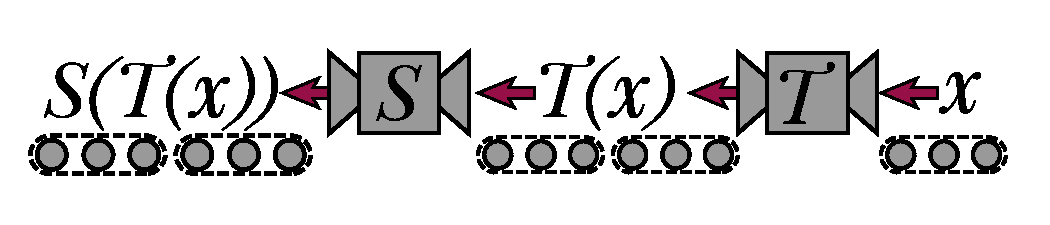
\includegraphics[scale=1]{Chapter3/images/SoT.pdf}}
%{\vspace{-10 pt}\hfill\footnotesize (Image contributed by Maria Langford)}\\ %Plagiarized?

\begin{Thm} Let $S : F^m\to F^p$ and $T : F^n \to F^m$ be linear transformations with standard matrices $A$ and $B$, respectively. Let $\bb x \in F^n$. Then 
\[S\circ T(\bb x) = S(T(\bb x)) = AB\bb x,\] that is, the matrix which represents the composite of two linear transformations is the product of their matrix representations.
\end{Thm}\vs

Recall that a linear transformation $T : F^n\to F^m$ is \emph{one-to-one} if and only if $T(\bb x) = T(\bb y)$ implies that $\bb x=\bb y$ if and only if $\ker T = \{\bb 0\}$, that is, the only vector mapping to zero is zero itself. Given the matrix representation $[T] = A$, we see that $\ker T = \null A$, that is, the vectors mapped to $\bb 0$ by $T$ are exactly those vectors whose product with $A$ is $\bb 0$. Hence, finding the null space of $A$ is equivalent to finding the kernel of $T$. In particular, a linear transformation is one-to-one if and only if the columns of its matrix representation are linearly independent.\\

\begin{Exam}\label{exam:transT} Let $T : \R^2 \to \R^3$ be a transformation given by the rule
\[T(x,y) = (x+y, 0, 2x+3y).\] Then 
\[[T] = \mtx{cc}{T(\bb e_1) & T(\bb e_2)} = \mtx{rr}{1&1\\0&0\\2&3} \sim \mtx{rr}{1&1\\2&3\\0&0} \sim \mtx{rr}{1&2\\0&1\\0&0} \sim \mtx{cc}{\fbox{$1$}&0\\0&\fbox{$1$}\\0&0}.\] The row-reduced echelon form of $[T]$ shows that the columns of $[T]$ are linear independent since there is  a pivot in each column. Therefore, $T$ is one-to-one, that is, $\ker T=\{\bb 0\}$.
\end{Exam}\vs

\begin{Exam}\label{exam:transS} Let $S : \R^3 \to \R^2$ be a linear transformation given by the rule 
\[S(x, y, z) = (x+y-2z, -y+z).\] Then 
\[[S] = \mtx{ccc}{S(\bb e_1) & S(\bb e_2) & S(\bb e_3)} = \mtx{rrr}{1&1&-2\\0&-1&1} \sim \mtx{rrr}{1&1&-2\\0&1&-1} \sim \mtx{ccr}{\fbox{$1$}&0&-1\\0&\fbox{$1$}&-1}.\] The row-reduced echelon form of $[S]$ shows that the columns of $[S]$ are linear dependent since there is no pivot in the third column. Therefore, $S$ is not one-to-one. In particular, $\ker S= \Span\{[1, 1, 1]^\top \}$.
\end{Exam}\vs

The homogeneous system $A\bb x = \bb 0$ has a nontrivial solution when $A$ has a non-pivot column. The nullity of $A$ is the number of non-pivot columns in $A$. If $A$ is an $m\times n$ matrix and $m<n$, that is, $A$ has more columns than rows, then $A$ necessarily has non-pivot columns. Hence, the $\text{nullity}(A) \ge 1$.\\

Recall that a linear transformation $T: F^n\to F^m$ is \emph{onto} if and only if for all vectors $\bb b\in F^m$ there exists a vector $\bb x\in F^n$ such that $T(\bb x) = \bb b$ if and only if $\im(T) = F^m$, that is, the set of images of $T$ is the whole target space $F^m$. Given the matrix representation $[T] = A$, we see that $\im  T = \col A$, that is, the vectors which are linear combinations of the columns of $A$ are exactly the vectors which can come out of $T$. Hence, finding the column space of $A$ is equivalent to finding the image of $T$. In particular, a linear transformation is onto if and only if the columns of its matrix representation span $F^m$.\\

\begin{Exam} Let $T : \R^2 \to \R^3$ be the transformation given in \examref{exam:transT}. The row-reduced echelon form of $[T]$ shows that $[T]$ has no pivot in the third row. Therefore, $T$ is not onto. In particular, $[0, 1, 0]^\top \notin \im T$.
\end{Exam}\vs

\begin{Exam} Let $S : \R^3 \to \R^2$ be the transformation given in \examref{exam:transS}. The row-reduced echelon form of $[S]$ shows that $[S]$ has a pivot in each row. Therefore, $S$ is onto. In particular, $\im S = \R^2$.
\end{Exam}\vs

The inconsistency of the equation $A\bb x=\bb b$ may occur when $A$ has a row of zeros in echelon form but the corresponding position in the augmented column is nonzero. In this case, consistency is dependent on the choice of $\bb b$ and at least one choice of $\bb b$ will make $A\bb x= \bb b$ inconsistent. These rows of zeros in the echelon form correspond to non-pivot rows of $A$. Let the \textbf{conullity} of $A$ denote the number of non-pivot rows of $A$.  If $A$ is an $m\times n$ matrix and $m>n$, that is, $A$ has more rows than columns, then $A$ necessarily has non-pivot rows. Hence, the $\text{conullity}(A) \ge 1$.\\

\begin{Prop} Let $T : F^n\to F^m$ is a linear transformation. 
\begin{enumerate}[!THM!]
\item If $m>n$, that is, $[T]$ has more rows than columns, then $T$ cannot be onto.
\item If $m<n$, that is, $[T]$ has more columns than rows, then $T$ cannot be one-to-one.
\end{enumerate}
\end{Prop}\vs

%%Every vector space can be expressed in coordinates making it essentially the same thing as $\R^n$. We say that $V$ and $\R^n$ are \textbf{isomorphic}, denoted $V\cong \R^n$, meaning that although the two spaces are different in their appearance and essentially the same shape. More precisely, an \textbf{isomorphism} is a bijective linear transformation. Such a mapping produces a one-to-one correspondence between vectors of the two spaces that preserves the algebraic structure. For example, the function $T : \P_n \to \R^{n+1}$ given by the rule
%%\[a_0 + a_1t + a_2t^2 + \ldots + a_nt^n \quad\longmapsto\quad \vr{a_0\\a_1\\a_2\\\vdots\\a_n}\] is an isomorphism. This means that $\P_n$ and $\R_{n+1}$ are essentially the same vector space.\\

%Let $V$ and $W$ be $n$- and $m$-dimensional vector spaces with bases $\B = \{\bb b_1, \ldots, \bb b_n\}$ and $\C = \{\bb c_1, \ldots, \bb c_m\}$, respectively. Let $T: V\to W$ be a linear transformation. Likewise, the coordinate mappings $[\cdot]_\B : V \to \R^n$ and $[\cdot]_\C : W \to \R^m$ are linear transformations (in fact, they are isomorphisms). Consider the composite linear transformation $([\cdot]_\C\circ T\circ [\cdot]_\B^{-1}) : \R^n\to \R^m$. This is a linear transformation between $\R^n$ and $\R^m$. Let $A$ be the standard matrix of this composite transformation. Then 
%\[[T(\bb x)]_\C = A[\bb x]_\B\] for all $\bb x\in V$. This matrix $A=  \,_\C[T]_\B$ is called the \textbf{standard matrix} of $T$ relative to $\B$ and $\C$. In fact, 
%\[A = \mtx{cccc}{[T(\bb b_1)]_\C & [T(\bb b_2)]_\C & \ldots & [T(\bb b_n)]_\C}.\] The matrix $\,_\C[T]_\B$ is sometimes called a \textbf{matrix representation} of the linear transformation $T$. The following diagram may be useful in remembering the relationship here:
%\begin{center}
%\begin{tikzpicture}
%\path (0,0) node (x) {$\bb x$};
%\path (x) ++ (3,0) node (Tx) {$T(\bb x)$};
%\path (x) ++ (0,-1.5) node (xB) {$[\bb x]_\B$};
%\path (xB) ++ (3,0) node (TxC) {$[T(\bb x)]_\c$};
%\draw[thick, ->] (x) -- (Tx) node[midway, above] {$T$};
%\draw[thick, ->] (xB) -- (TxC) node[midway, above] {$A$};
%\draw[thick, ->]  (x) -- (xB);
%\draw[thick, ->]  (Tx) -- (TxC);
%\end{tikzpicture}
%\end{center}
%
%\begin{Exam}Suppose $\B = \{\bb b_1, \bb b_2\}$ is a basis for $V$ and $\C = \{\bb c_1, \bb c_2, \bb c_3\}$ is a basis for $W$. Let $T : V\to W$ be a linear transformation such that 
%\[T(\bb b_1) = 3\bb c_1 - 2\bb c_2 + 5\bb c_3\qquad T(\bb b_2) = 4\bb c_1 + 7\bb c_2 - \bb c_3.\] Then 
%\[[T(\bb b_1)]_\C =  \vr{3\\-2\\5}\qquad\text{and}\qquad [T(\bb b_2)]_\C =  \vr{4\\7\\-1}.\] This gives
%
%\[A = \mtx{cc}{[T(\bb b_1)]_\C & [T(\bb b_2)]_\C} =\mtx{rr}{3&4\\-2&7\\5&-1}.\qedhere\]
%\end{Exam}\vs
%
%When $T : V \to V$ is a linear transformation with the same domain and codomain, we often use the same basis for the domain and codomain. \\

%%\begin{Exam} The mapping $D : \P_2 \to \P_2$, defined by 
%%\[D(a_0+a_1t+a_2t^2) = a_1+2a_2t,\] is linear (this is just the derivative). \\
%%\begin{enumerate}[(a)]
%%\begin{multicols}{2}
%%\item Find the standard matrix of $D$ relative to $\B$, where $\B = \{1, t,t^2\}$.\\
%%
%%Since $D(1) = 0$, $D(t) = 1$, and $D(t^2) = 2t$, we have that:  \columnbreak
%%\[[D]_\B = \mtx{rrr}{0&1&0\\0&0&2\\0&0&0}.\]
%%\end{multicols}\vs
%%
%%\item Verify that $[D(\bb p)]_\B = [D]_\B[\bb p]_\B$ for all $\bb p\in \P_2$.\\
%%
%%Let $\bb p(t) = a_0+a_1t+a_2t^2$. Then  $[\bb p]_\B = \vr{a_0\\a_1\\a_2}$ and $[D]_\B[\bb p]_\B = \mtx{rrr}{0&1&0\\0&0&2\\0&0&0}\vr{a_0\\a_1\\a_2} = \vr{a_1\\2a_2\\ 0}.$ On the other hand, $[D(\bb p(t)]_\B = [a_1+2a_2t]_\B = \vr{a_1\\2a_2\\0}.$ Therefore, the two forms agree. \hfill$\qedhere$
%%\end{enumerate}
%%\end{Exam}
%
%%Let $\B = \{\bb v_1, \ldots, \bb v_n\}$ be a basis for a vector space $V$. Let $\bb x, \bb y\in V$ such that 
%%\[\bb x= c_1\bb v_1 + \ldots + c_n\bb v_n\quad\text{and}\quad \bb y= d_1\bb v_1 + \ldots + d_n\bb v_n.\] Then
%%\[[\bb x]_\B = \mtx{c}{c_1\\\vdots\\c_n}\quad\text{and}\quad[\bb y]_\B = \mtx{c}{d_1\\\vdots\\d_n}.\] Thus, 
%%\[[\bb x + \bb y]_\B = [(c_1+d_1)\bb v_1+\ldots + (c_n+d_n)\bb v_n]_\B = \mtx{c}{c_1+d_1\\\vdots\\c_n+d_n} = \mtx{c}{c_1\\\vdots\\c_n} + \mtx{c}{d_1\\\vdots\\d_n} = [\bb x]_\B + [\bb y]_\B.\] Likewise, for any $r\in \R$, 
%%\[[r\bb x]_\B = [rc_1\bb v_1 + \ldots + rc_n\bb v_n]_\B =  \mtx{c}{rc_1\\\vdots\\rc_n} = r\mtx{c}{c_1\\\vdots\\c_n} = r[\bb x]_\B.\] Therefore, the change-of-coordinates map $[\cdot]_\B : V \to \R^n$ is a linear transformation. In fact, it is even bijective (it maps a basis onto a basis). 
%%
%%\begin{Thm}[Theorem 8] Let $\B = \{\bb b_1, \ldots, \bb b_n\}$ be a basis for a vector space $V$. Then the coordinate mapping $\bb x \mapsto [\bb x]_\B$ is an isomorphism, that is, a bijective linear transformation.
%%\end{Thm}\vs
%%
%%Of special interest is the case when $V = \R^n$, because we can then compute the standard matrix of $[\cdot]_\B$. Let the \textbf{change-of-coordinates matrix} 
%%\[P_\B = \mtx{cccc}{\bb b_1 & \bb b_2 & \ldots & \bb b_n}\] be defined. Then 
%%\[\bb x = P_\B[\bb x]_\B\] for all $\bb x\in \R^n$, and \[P_\B^{-1}\bb x = [\bb x]_\B.\]\vs
%
%%\begin{Def} Suppose the set $\B = \{\bb v_1, \bb v_2, \ldots, \bb v_n\}$ is a basis for a vector space $V$. For each $\bb x\in V$, the \textbf{coordinates of $\bb x$ relative to the basis $\B$} are the weights $c_1, \ldots, c_n$ such that 
%%\[\bb x = c_1\bb v_1 + c_2\bb v_2 +\ldots + c_n\bb v_n.\] The vector in $\R^n$
%%\[[\bb x]_\B = \mtx{c}{c_1\\\vdots\\c_n}\] is called the \textbf{coordinate vector of $\bb x$ relative to $\B$} or the \textbf{$\B$-coordinate vector of $\bb x$}.
%%\end{Def}\vs 
%
%%So even in abstract settings, linear transformations are nothing more than just matrices. In fact, the kernel of a linear transformation in coordinates is just the null space of its matrix representation. Likewise, the range of the transformation in coordinates just the column space of the matrix representation. As we have seen before with matrix transformations $T : \bb x \mapsto A\bb x$ for an $m\times n$ matrix $A$, the columns of $A$ span $\R^m$ if and only if $T$ is onto and the columns of $A$ are linearly independent if and only if $T$ is one-to-one. Combining this with the Basis Theorem, which says that if a spanning set or linearly independent set have the same size as the dimension then it is a basis, we get more conditions equivalent to nonsingularity.
%%

%%%%%%%%%%%%%%%%%% Exercises %%%%%%%%%%%%%%%%%%%
\startExercises{representation}

\noindent For Exercises \ref{exer:standardmatrixstart}-\ref{exer:standardmatrixstop}, for the linear transformations $T$ find its standard matrix $[T]$.%NEW
\begin{enumerate}[!HW!, start=1, label=$\spadesuit$ \arabic*., ref=\arabic*]
\item\label{exer:standardmatrixstart} $T : \R^2\to \R^2 : T(x_1,x_2) = (2x_1-x_2, -4x_2)$.
\itemspade $T : \R^3\to \R^4 : T\left(\vr{x_1\\x_2\\x_3}\right) = \mtx{c}{x_1+2x_2+x_3\\ 3x_1+14x_3-5x_2 \\  3x_2 - 5x_1-18x_3 \\ 19x_2-7x_1-40x_3}$.
\itemspade $T : \C \to \C^4 : T(z) = (z, iz, -z, -iz)$.
\itemspade $T : \Z_2^4 \to \Z_2 : T(x_1, x_2, x_3, x_4) = x_1+x_2+x_3+x_4$.
\item\label{exer:standardmatrixstop}  $T : \Z_5^3\to \Z_5^3 : T(x_1,x_2,x_3) = (x_3, x_2, x_1)$.
\end{enumerate}

\noindent For Exercises \ref{exer:standardmatrixcompositestart}-\ref{exer:standardmatrixcompositestop}, find the standard matrix of the composite function $S\circ T$. %NEW
\begin{enumerate}[!HW!, label=$\spadesuit$ \arabic*., ref=\arabic*]
\item\label{exer:standardmatrixcompositestart}\label{exer:standardmatrixcompositestop}
$T : \R^2 \to \R^3 : T(x_1,x_2) = (2x_2, 3x_1, 2x_1-3x_2)$ and $S : \R^3\to \R^2 : S(y_1, y_2, y_3) = (y_3-2y_2, y_1-2y_3)$
\end{enumerate}

\noindent For Exercises \ref{exer:standardmatrixnullstart}-\ref{exer:standardmatrixnullstop}, determine if the given linear transformation from Exercises \ref{exer:standardmatrixstart}-\ref{exer:standardmatrixstop} is one-to-one or onto. Find a basis for its kernel and for its image.%NEW
\begin{enumerate}[!HW!, label=$\spadesuit$ \arabic*., ref=\arabic*]
\begin{multicols}{5}
\item\label{exer:standardmatrixnullstart}
Exercise \ref{exer:standardmatrixstart}
\itemspade \FPeval{\result}{clip(\getrefnumber{exer:standardmatrixstart}+1)} Exercise \result
\itemspade \FPeval{\result}{clip(\getrefnumber{exer:standardmatrixstart}+2)} Exercise \result
\itemspade \FPeval{\result}{clip(\getrefnumber{exer:standardmatrixstart}+3)} Exercise \result
\item\label{exer:standardmatrixnullstop}  Exercise \ref{exer:standardmatrixstop}\
\end{multicols}
\end{enumerate}

\noindent QUICK! For Exercises \ref{exer:standardmatrixnullstart}-\ref{exer:standardmatrixnullstop}, determine in less than 10 seconds if the linear transformation CANNOT be one-to-one and if it CANNOT be onto. 
\begin{enumerate}[!HW!]
\item $T : \R^3\to \R^3 : T(x,y,z)=(x,y,z)$ %Jacob Kuhn
\item $T: \R^3\to \R^2 : T(x_1,x_2,x_3)=(x_1+2x_2, x_3-3x_2)$ %Daven Triplett
\item $T: \R^3\to \R^4 : T(x_1,x_2,x_3)=(2x_1+3x_3, x_2+4x_1+x_3, x_3+x_1+x_2, x_1+3x_2+x_3)$ %Daven Triplett
\item $T: \C \to \C^3 : T(z) = (z,z,z)$%Jacob Kuhn
\item $T:\C\to \C^3 : T(z) = ((3-i)z, (-2+2i)z, z)$ %Daven Triplett
\item $T: \Z_5^3 \to \Z_5 : T(x,y,z) = x+y+z$%Jacob Kuhn
\item $T: \Z_7^2\to \Z_7^2 : T(x,y)=(4x+2y, 3y)$ %Daven Triplett
\end{enumerate}

%%%%%%%%%%%%%%%%%%% Footnotes %%%%%%%%%%%%%%%%%%%
 %\mbox{}\vfill%3.7 Representations of Linear Transformations

%%%% Chapter 4 %%%%%%
\chapter{Orthogonality}\label{chap:ortho}
In this chapter, we will begin to develop the geometric framework of lengths and angles through the lens of linear algebra. While the notions of affine geometry were introduced earlier in \chapref{chap:vectors}, this chapter will develop the notions of Euclidean geometry. As such, this geometric development will not be entirely possible for the finite fields $\Z_p$ we have often considered, although some notion of orthogonality are available for general fields. In this chapter the only fields $F$ we will consider for scalars will be $\R$ and $\C$. \\

\begin{center}
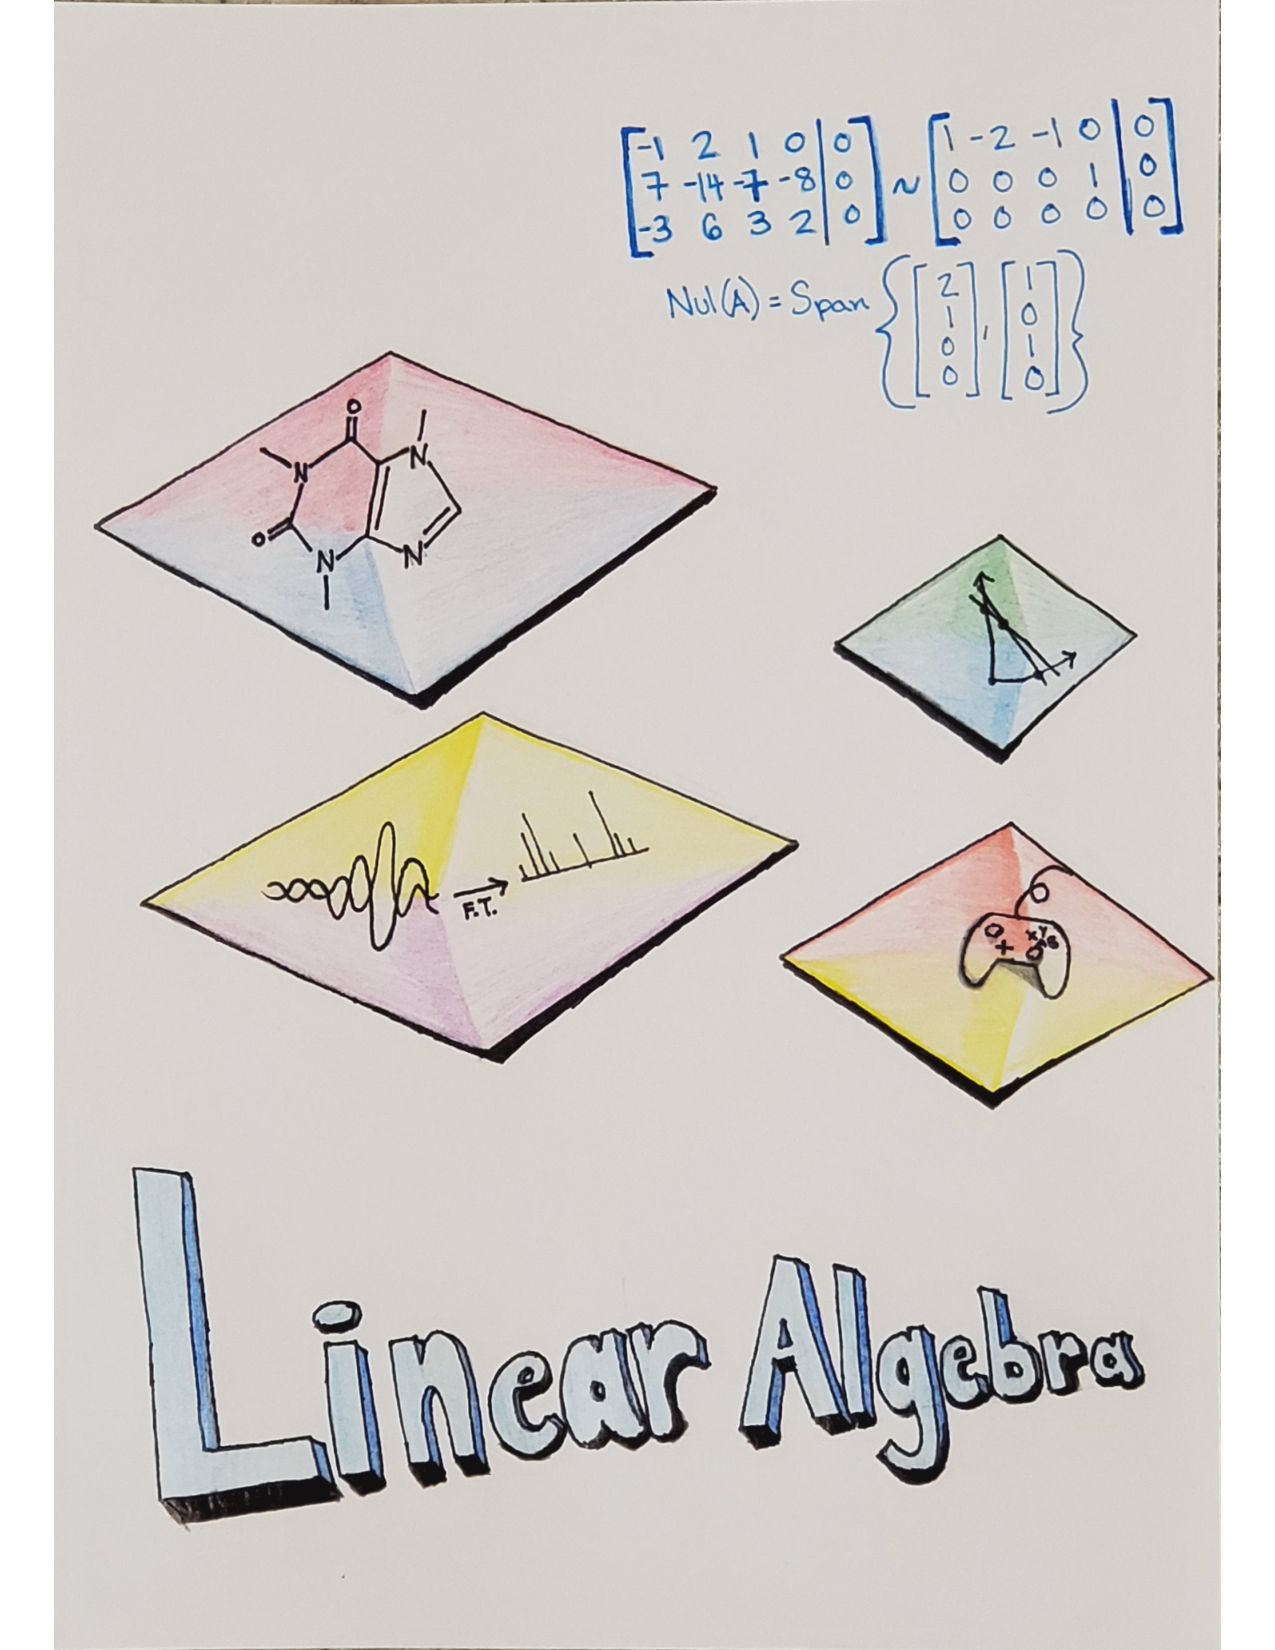
\includegraphics[scale=0.75, trim = 40 255 29 45, clip]{Chapter4/images/Chapter4cover.pdf}%Mariah Clayson
\end{center}
%{\vspace{-10 pt}\hfill\footnotesize (Drawing contributed by Mariah Clayson)}\\ %The main focus of the design is the four basic shapes in the center, representing the Fundamental Theorem of Linear Algebra. Inside of each of the parallelograms is a representation of real life linear algebra applications. Starting with the top left, this caffeine molecule is to represent the use of linear algebra in balancing chemical equations, solving for concentrations in systemic treatments of equilibrium, and solving for absorbance values particularly in UV-vis when several different molecules are in the solution. The bottom left picture is a representation of a Fourier Transform which is typically used to convert a time domain to a frequency domain, especially in NMR (Nuclear Magnetic Resonance spectroscopy) which is used to identify compounds in chemical labs. The top right figure is a representation of linear programming that can be used to find optimal solutions in a variety of settings. The bottom right picture is meant to represent video games and 3D graphics in general as they are a projection of three dimensional components onto a two-dimensional screen. The top most component of the cover art is an example of matrices being used to calculate the null space. The title itself is also meant to be a ``3D” image that represents linear algebra’s usefulness in this area.

\pagebreak  %Orthogonality

\begin{center} 
\emph{``Success isn't measured by money or power or social rank. Success is measured by your discipline and inner peace.'' -- Mike Ditka}
\end{center}

\section{Inner Products}\label{sec:inner}
\begin{Def} We define the \textbf{dot product} $\cdot : \R^n\times \R^n \to \R$ of two vectors, $\bb u, \bb v \in \R^n$ by the rule
\[\bb u \cdot \bb v = \bb u^\top \bb v = \mtx{cccc}{u_1 & u_2 & \ldots & u_n}\mtx{c}{v_1 \\ v_2 \\ \vdots \\ v_n} = u_1v_1 + u_2v_2 + \ldots + u_nv_n.\]
\end{Def}\vs

\begin{Exam} Given $\bb u = \vr{1\\2\\3}$ and $\bb v = \vr{-5\\0\\3}$, their dot product is 
\[\bb u \cdot \bb v = 1(-5)) +2(0) + 3(3) = -5 +0 + 9 = \fbox{$4$}. \qedhere\]
\end{Exam}\vs

Let $A$ be an $m\times n$ matrix and let $\bb x\in \R^n$. Let $\bb r_1, \bb r_2,\ldots, \bb r_m\in \R^n$  be the row vectors of $A$. Thus,

$A = \mtx{c}{\bb r_1\\ \bb r_2\\ \vdots \\ \bb r_m}$. Then we can define the matrix-vector product using dot products: $A\bb x = \mtx{c}{\bb r_1\cdot \bb x\\ \bb r_2\cdot \bb x \\ \vdots\\ \bb r_m\cdot \bb x}.$\\\\

There are many algebraic reasons to extend the dot product over other fields, such as $\Z_p$ and $\C$, like in the above redefinition of matrix multiplication. For another example, the dot product is used in the creation of error-correcting codes which involved vectors of $\Z_2^n$, but the geometric benefits of the dot product are absent on these fields and this is the very goal of this chapter. Furthermore, over complex vector spaces, we vowed to never use the matrix transpose $\mbox{}^\top $. Instead, we use the conjugate transpose $\mbox{}^*$. The reason we made such a vow will be presented below in this section. This changes how we compute dot products of complex vectors.\\

\begin{Def}
We define the \textbf{Hermitian product}\footnotemark[2] $\cdot : \C^n\times \C^n \to \C$ of two vectors, $\bb u, \bb v \in \C^n$ by the rule
\[\bb u \cdot \bb v = \bb u^* \bb v = \mtx{cccc}{\overline{u_1} & \overline{u_2} & \ldots & \overline{u_n}}\mtx{c}{v_1 \\ v_2 \\ \vdots \\ v_n} = \overline{u_1}v_1 + \overline{u_2}v_2 + \ldots + \overline{u_n}v_n.\]
\end{Def}\vs



\begin{Exam} Let $\bb u = (1+i,\ i,\ 3-i)$ and $\bb v = (1+i,\ 2,\ 4i)$. Find $\bb u\cdot \bb v$ and $\bb v\cdot \bb u$.%, and $\Vert \bb u\Vert$.

\[\bb u\cdot \bb v = (\overline{1+i})(1+i) + \overline{i}(2) + (\overline{3-i})(4i) = (1-i)(1+i) - 2i + (3+i)(4i) = 2 - 2i + 12i - 4 = \fbox{$-2+10i$}\]
\[\bb v \cdot \bb u = (\overline{1+i})(1+i) + \overline{2}(i) + (\overline{4i})(3-i) = (1-i)(1+i) + 2i - (4i)(3-i) = 2 + 2i - 12i - 4 = \fbox{$-2 - 10i$}\]
%\[\Vert \bb u\Vert = \sqrt{(\overline{1+i})(1+i) + (\overline{i})i + (\overline{3-i})(3-i)} = \sqrt{ (1-i)(1+i) + (-i)i + (3+i)(3-i)} = \sqrt{2 + 1 + 10} = \fbox{$\sqrt{13}$}\qedhere\]
\end{Exam}\vs

Note that since $\R^n\subseteq \C^n$ and $\overline{x} = x$ whenever $x\in \R$, the definition of the Hermitian product generalizes the notion of the dot product. But as the dot product is a possible operation on $\C^n$ (and there are situations where one might allow the dot product of complex vectors), we will not refer to this generalization as the dot product, but instead as the Hermitian product. Both the dot product over $\R^n$ and the Hermitian product over $\C^n$ will be denoted $\bb u \cdot \bb v$. In an attempt to unify the vocabulary here, we will call the dot product on $\R^n$ and the Hermitian product on $\C^n$ the (standard) \textbf{inner product}\footnotemark[8] on $F^n$, where $F$ could be $\R$ or $\C$. \\

\begin{Thm}\label{thm:inner} Let $F$ be $\R$ or $\C$. Let $\bb u, \bb v, \bb w\in F^n$ and let $c\in F$. Then

\begin{enumerate}[!THM!,start=1]
\begin{multicols}{2}
\item\label{2nd} $\bb u \cdot(\bb v + \bb w) = \bb u \cdot \bb v  + \bb u \cdot \bb w$;
\item\label{3rd} $\bb u\cdot (c\bb v) = c(\bb u\cdot \bb v)$;
\end{multicols}
\begin{multicols}{2}
\item\label{1st} $\bb u \cdot \bb v = \bb v \cdot \bb u$;
\item\label{4th} $\bb u \cdot \bb u \ge 0$, and $\bb u \cdot \bb u = 0$ if and only if $\bb u = \bb 0$.
\end{multicols}
\end{enumerate}
\end{Thm}
%\begin{proof}
%We will prove part \emph{(\ref{2nd})}. Let $\bb u = (u_1, \ldots, u_n)$, $\bb v = (v_1, \ldots, v_n)$, and $\bb w = (w_1, \ldots, w_n)$. Then 
%\begin{eqnarray*}
%(\bb u + \bb v)\cdot \bb w &=& (u_1+v_1,\ldots, u_n+v_n)\cdot \bb w = (u_1+v_1)w_1 + \ldots + (u_n+v_n)w_n\\
% &=& u_1w_1 + v_1w_1 + \ldots + u_nw_n + v_nw_n = (u_1w_1 + \ldots + u_nw_n) + (v_1w_1 + \ldots + v_nw_n)\\
% &=& \bb u\cdot \bb w + \bb v \cdot \bb w.
%\end{eqnarray*}
%
%The remaining properties are proved similarly.
%\end{proof}\vs
Properties \ref{2nd} and \ref{3rd} above show us that inner multiplication on the left is a linear transformation $F^n\to F$ for each fixed vector $\bb u\in F^n$. When $F=\R$, \ref{1st} simplifies to just be $\bb u\cdot \bb v=\bb v\cdot \bb u$, that is, the dot product is \emph{symmetric}. Combining all these three properties shows that $(\bb u+\bb v)\cdot \bb w = \bb u\cdot \bb w + \bb v\cdot \bb w$ and $(c\bb u)\cdot \bb v = c(\bb u\cdot \bb v)$ whenever $\bb u, \bb v, \bb w\in \R^n$ and $c\in \R$. Thus, the dot product is linear in the first factor and linear in the second factor, that is, we say the dot product is \emph{bilinear}. These properties derive from the properties of transposition.\\

Conversely, the Hermitian product is \emph{conjugate-symmetric}, that is, the vector commute at the price of complex conjugation, as shown in \ref{1st}. As such, inner multiplication on the right is not exactly a linear transformation. Like with the real vector spaces, $(\bb u+\bb v)\cdot \bb w = \bb u\cdot \bb w + \bb v\cdot \bb w$ still holds for all $\bb u, \bb v, \bb w\in \C^n$. On the other hand, we get $(c\bb u)\cdot \bb v= \overline{c}(\bb u\cdot \bb v)$, that is, we can only factor scalars from the first factor if we take their conjugate. Thus, the Hermitian product is linear in the second factor and \emph{conjugate-linear} in the second factor, that is, we say the Hermitian product is \emph{sequilinear}. These properties derive from the properties of transposition.\\

Lastly, \ref{4th} is commonly referred to as \emph{positive-definite property}\footnotemark[3], \emph{positive} because $\bb x\cdot \bb x\ge 0$ and \emph{definite} because $\bb u\cdot \bb u=0$ if and only if $\bb u=0$. 



\begin{Def} The \textbf{length} (or \textbf{norm}) of a vector $\bb v\in F^n$ is the nonnegative scalar $\Vert \bb v\Vert$ defined by
\[\Vert \bb v\Vert = \sqrt{\bb v\cdot \bb v} = \sqrt{v_1^2+v_2^2 + \ldots + v_n^2}.\] We say that $\bb v$ is a \textbf{unit vector} if $\Vert \bb v\Vert = 1$.
\end{Def}\vs

It is useful to note that $\Vert \bb v\Vert^2 = \bb v\cdot \bb v$.\\

\begin{Thm} Let $\bb u%, \bb v 
\in F^n$ and $c\in F$. Then 
%\begin{enumerate}[!THM!, start=1]
%\begin{multicols}{2}
%\item $\Vert \bb u+\bb v\Vert \le \Vert \bb u\Vert + \Vert \bb v\Vert$;
%\item 
$$\Vert c\bb v\Vert = |c|\Vert \bb v\Vert$$
%\end{multicols}
%\item $\Vert\bb u\Vert \ge 0$, and $\Vert \bb u\Vert = 0$ if and only if $\bb u=\bb 0$.
%\end{enumerate}
\end{Thm}\vs
%\begin{proof}
%First of all,
%\[\Vert c\bb v\Vert^2 = (c\bb v)\cdot(c\bb v) = c(\bb v \cdot (c\bb v)) = c^2(\bb v \cdot \bb v) = (|c|(\bb v \cdot \bb v))^2 = (|c|\Vert \bb v\Vert)^2.\] To finish, take square roots.
%\end{proof}\vs

\begin{Exam} Let $\bb v = \vr{1\\0\\2\\-2} \in \R^4$. Then the length of $\bb v$ is 
\[\Vert \bb v\Vert = \sqrt{\bb v\cdot \bb v} = \sqrt{1(1) + 0(0)+ 2(2) -2(-2) } = \sqrt{1+4+4} = \sqrt{9} = \fbox{$3$}.\] Since the length of $\bb v$ is 3, $\bb v$ is not a unit vector. On the other hand, let $\bb u = \dfrac{1}{3}\bb v = \mtx{c}{1/3\\0\\2/3\\ -2/3}$. Then 
\[\Vert \bb u\Vert = \left\Vert \frac{1}{3} \bb v\right\Vert = \frac{1}{3}\Vert \bb v\Vert = \frac{1}{3}(3) = \fbox{$1$}.\] Therefore, $\bb u$ is a unit vector in the same direction as $\bb v$.
\end{Exam}\vs

The process of constructing a unit vector in the same direction as a given vector is called \textbf{normalization}. The normalization of any nonzero vector $\bb v$ is given by $\dfrac{1}{\Vert \bb v\Vert}\bb v$. The zero vector cannot be normalized. In particular, the zero vector does not point in any direction.\\

\begin{Exam} Let $\bb u = (1+i,\ i,\ 3-i)$. Find  $\Vert \bb u\Vert$.

\[\Vert \bb u\Vert = \sqrt{(\overline{1+i})(1+i) + (\overline{i})i + (\overline{3-i})(3-i)} = \sqrt{ (1-i)(1+i) + (-i)i + (3+i)(3-i)} = \sqrt{2 + 1 + 10} = \fbox{$\sqrt{13}$}\qedhere\]
\end{Exam}\vs

\begin{Def} For $\bb u, \bb v\in F^n$, the \textbf{distance} between $\bb u$ and $\bb v$, denoted as $\dist(\bb u, \bb v)$, is the length of the vector $\bb u -\bb v$, that is, 
\[\dist(\bb u, \bb v) = \Vert \bb u-\bb v\Vert.\]
\end{Def}\vs

\begin{Exam} Let $\bb u = \vr{7\\1}$ and $\bb v = \vr{3\\2}$. Then
\[\dist(\bb u, \bb v) = \Vert \bb u - \bb v\Vert = \left\Vert \vr{4\\-1}\right\Vert = \sqrt{4^2+(-1)^2} = \fbox{$\sqrt{17}$}. \qedhere\]
\end{Exam}\vs

%In physics, \textbf{work} is a force $\bb F$ applied over a distance $\bb d$. Intuitively, work is a measure of effort expended when moving an object by applying a force to it. Unlike velocity and force, work is a scalar.\\
%
%\begin{Thm} If a constant force $\bb F$ is applied to an object and moves the object in a straight line a distance $\bb d$, then the work $W$ performed by the force is 
%\begin{equation} W = \bb F\cdot \bb d\end{equation} where $\theta$ is the angle between the force $\bb F$ and $\bb d$.
%\end{Thm}\vs
%
%\begin{Exam} A force $\bb F =  35\bb i-12\bb j$ (in pounds) is used to push an object up a ramp. The resulting movement of the object is represented by the displacement vector $\bb d = 15\bb i +4\bb j$ (in feet). Find the work done by the force.\\
%\begin{center}
%\begin{tikzpicture}
%\draw[thick] (0,0) --  ++(15/20,4/20) -- ++(-4/20, 15/20) -- ++(-15/20,-4/20) -- cycle;
%\draw[thick] (0,0) -- (15/4,4/4);
%\draw[thick, dashed] (-1,0) -- (15/4,0);
%\draw[ultra thick, red, ->] (15/40, 19/40)++(0,0) -- ++(15/10,4/10) node[ above] {$\bb d$};
%\draw[ultra thick, blue, ->] (15/40, 19/40)++(0,0) -- ++(35/10,-12/10) node[midway, below] {$\bb F$};
%\end{tikzpicture}
%\end{center}
%\[\text{Work} = \bb F\cdot \bb d  = 35(15) + (-12)(4) = 525-48 = \fbox{480 ft-lb}\]
%\end{Exam}

%%%%%%%%%%%%%%%%%% Exercises %%%%%%%%%%%%%%%%%%%
\startExercises{inner}

\noindent For Exercises \ref{exer:computerdotstart}-\ref{exer:computerdotstop}, compute the given quantity. 
\begin{enumerate}[!HW!, start=1]
\begin{multicols}{3}
\item\label{exer:computerdotstart} Compute $3\bb u\cdot 2\bb v$, if \\ $\bb u =\vr{1\\ -2}$, $\bb v=\vr{2\\-3}$\columnbreak % Anthony Nguyen
\itemspade Compute $\bb u\cdot \bb v$, if\\ $\boldsymbol{u} = \vr{ 1\\ -1}$, $\boldsymbol{v} = \vr{2\\ -3}$ \columnbreak %Albert Dot Product: Basic Computation in R^2
\itemspade Compute $\bb u\cdot \bb v$, if\\ $\boldsymbol{u} = \vr{ 7\\ 1\\ -5}$, $\boldsymbol{v} = \vr{1\\ -1\\ 2}$ %Albert Dot Product: Basic Computation in R^3
\end{multicols}
\begin{multicols}{3}

\itemspade Compute $\bb u\cdot \bb v$, if\\ $\boldsymbol{u}=\vr{ 2\\ 1\\ -3\\ 2}$, $\boldsymbol{v} = \vr{ 7\\ 1\\ -1\\ 2}$\columnbreak %Albert Dot Product: Basic Computation in R^4
\item Compute $5\bb u\cdot 2\bb v$, if\\ $\bb u =\vr{7\\1\\-5}$,  $\bb v=\vr{1\\-1\\2}$\columnbreak  %Anthony Nguyen
\item Compute $2\bb u\cdot 3\bb v$, if\\ $\bb u =\vr{7\\1\\-3\\2}$, $\bb v=\vr{7\\1\\-1\\2}$ %Anthony Nguyen
\end{multicols}

\begin{multicols}{2}
\itemspade Compute $\bb u\cdot \bb v$, $\bb u\cdot \bb w$, and $\bb v\cdot \bb w$, if\\
$\bb u = \vr{i\\ 2i\\3i}$, $\bb v = \mtx{c}{4\\-2i\\ 1+i}$, $\bb w = \mtx{c}{2-i\\ 2i\\ 5+3i}$\columnbreak %Anton 5.3.11, 12 p. 324
\itemspade Compute $\bb u\cdot \bb v$, $\bb u\cdot \bb w$, and $\bb v\cdot \bb w$, if\\
\mbox{}\hspace{-20 pt}$\bb u = \mtx{c}{1+i\\ 4\\ 3i}$, $\bb v = \mtx{c}{3\\-4i\\2+3i}$, $\bb w = \mtx{c}{1-i\\ 4i\\ 4-5i}$%Anton 5.3.11, 12 p. 324
\end{multicols}

\begin{multicols}{2}
\itemspade Compute $(\boldsymbol{u} +  \boldsymbol{v}) \cdot \boldsymbol{w}$, if\\ $\boldsymbol{u} = \vr{ 1\\ -5\\ 0}$, $\boldsymbol{v} = \vr{ 3\\ 2\\ -3}$, and $\boldsymbol{w} = \vr{ 1\\ 0\\ -1}$\columnbreak %Albert Dot Product Properties: Order of Operations with Vector Sums
\itemspade Compute $2\boldsymbol{u} \cdot ( \boldsymbol{v} + \boldsymbol{w})$, if\\ $\boldsymbol{u} = \vr{ -1\\ -1\\ 3}$, $\boldsymbol{v} = \vr{ 1\\ -2\\ 1}$, $\boldsymbol{w} = \vr{ 0\\ -5\\ 3}$ %Albert Dot Product: Computation with a Vector Sum and a Scalar Multiple
\end{multicols}
\itemspade Find $(A\boldsymbol{u})\cdot \boldsymbol{v}$ where $A= \mtx{ccc}{ 1&2&3\\ 0&-1&-1\\ 1&0&1}$, $\boldsymbol{u} = \vr{ -2\\ 1\\ -1}$, $\boldsymbol{v} = \vr{ -1\\ -1\\ 3}$ %Albert Dot Product: Computation with a Matrix Product

\begin{multicols}{4}
\itemspade Compute $\Vert\bb u\Vert$, if\\ $\boldsymbol{u} = \vr{ 7\\ 1\\ 5}$\columnbreak %Albert Vector Norm: Basic Computation in R^3
\itemspade Compute $\Vert\bb u\Vert$, if\\ $\boldsymbol{u} = \vr{2\\ 1\\ -3\\ 2}$\columnbreak %Vector Norm: Basic Computation in Four Dimensions

\itemspade Compute $\Vert\bb u\Vert$, if\\ $\bb u = \mtx{c}{2-i\\ 4i\\ 1+i}$\columnbreak

\itemspade Compute $\Vert\bb u\Vert$, if\\ $\bb u = \mtx{c}{6\\ 1+4i\\ 6-2i}$
\end{multicols}

\itemspade Compute $\dist(\bb u, \bb v)$, if\\ $\boldsymbol{u} = \vr{ 1\\ 1\\ 1}$,  $\boldsymbol{v} = \vr{5\\ 2\\ 2}$ %Albert Vector Distance: Distance in 3-space


\itemspade Compute $\dist(\bb u-\bb v, 2\bb w + \bb x)$, if\\ $\boldsymbol{u} = \vr{ 1\\ -2\\ 1}$, $\boldsymbol{v} = \vr{ 0\\ -5\\ 3}$, $\boldsymbol{w} = \vr{ 3\\ -1\\ -2}$,  $\boldsymbol{x} = \vr{ 0\\ 1\\ 0}$ %Albert Vector Distance: Between Linear Combinations

\item\label{exer:computerdotstop} Compute $\dist((\boldsymbol{u} \cdot \boldsymbol{v})\boldsymbol{w}, 2\boldsymbol{x})$, if\\ $\boldsymbol{u} = \vr{ 3\\ -1\\ -2}$, $\boldsymbol{v} = \vr{ 1\\ -2\\ 3}$, $\boldsymbol{w} = \vr{ -2\\ 1\\ -1}$, $\boldsymbol{x} = \vr{ 0\\ 1\\ 0}$ %Albert Vector Distance: Between Scalar Multiples Involving Dot Products
\end{enumerate}

\begin{enumerate}[!HW!]
\begin{multicols}{2}
\item Find $x$ such that $\vr{ 1\\ 1\\ x} \cdot \vr{ x\\ 2\\ -3} = 1$. %Albert Dot Product: Computation with Variable Coordinates

\item For which real numbers $x$ make $\vr{ 1/2 \\ 1/3 \\ x }$ a unit vector? %Albert Unit Vector: One Unknown Coordinate
\end{multicols}
\end{enumerate}

%%%%%%%%%%%%%%%%%%% Footnotes %%%%%%%%%%%%%%%%%%%
 \mbox{}\vfill
 
 \footnotetext[2]{Many textbooks alternatively define the Hermitian product as $\bb u \cdot \bb v =  \bb u^\top \overline{\bb v}$. Although this does not at all change the theory and applications of the Hermitian product, it does change intermediate calculations. Be cautious if comparing with other sources since there is no universal consensus.}
 
 \footnotetext[8]{More generally, an \emph{inner product} on $F^n$ is any function $F^n\times F^n\to F$ which satisfies the axioms of \thmref{thm:inner}.}
 
 \footnotetext[3]{This property is the reason we will not be considering finite fields in this chapter. The dot product over any field is always symmetric and bilinear. The positive-definite condition fails for these fields and many others. Positive-definition is needed to establish the geometric properties we seek.}
\pagebreak%4.1 Inner Products %CLEAN
\begin{center} 
\emph{``To be trusted is a greater compliment than being loved.'' -- George MacDonald}
\end{center}

\section{Orthogonality}\label{sec:ortho}
\centerline{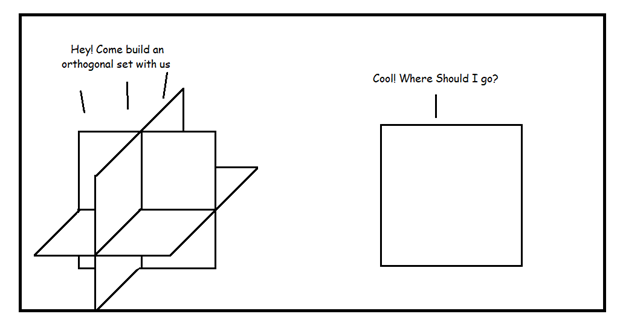
\includegraphics[scale=0.75]{Chapter4/images/orthocomic.png}}
%{\vspace{-10 pt}\hfill\footnotesize (Image contributed by Thayne Hansen)}\\
\begin{Def} Two nonzero\footnotemark[2] vectors $\bb u, \bb v\in F^n$ are \textbf{orthogonal} if $\bb u\cdot \bb v=0$.
\end{Def}\vs

\begin{Exam} Given the vectors $\bb u = \vr{1\\2\\3}$, $\bb v= \vr{1\\1\\-1}$, and $\bb w = \vr{2\\3\\5}$, determine if $\bb u$ is orthogonal to $\bb v$ or $\bb w$.\\
\[\bb u \cdot \bb v = 1(1)+2(1)+3(-1) = 3-3 = 0.\] Thus, $\bb u$ is orthogonal to $\bb v$. 
\[\bb u \cdot \bb w = 1(2)+2(3)+3(5) = 23\neq 0.\] Thus, $\bb u$ is not orthogonal to $\bb w$.
\[\bb v \cdot \bb w = 1(2)+1(3)-1(5) = 5-5 = 0.\] Thus, $\bb v$ is orthogonal to $\bb w$. 
\end{Exam}\vs

\begin{Thm}[Pythagorean Theorem] \label{thm:pythagorean}
Two vectors $\bb u, \bb v\in F^n$ are orthogonal\footnotemark[8] then \[\Vert \bb u + \bb v\Vert^2 = \Vert \bb u\Vert^2+ \Vert \bb v\Vert^2.\]
\end{Thm}
%\begin{Thm}[Pythagorean Theorem] 
%Two vectors $\bb u, \bb v\in V$ are orthogonal if and only if \[\Vert \bb u + \bb v\Vert^2 = \Vert \bb u\Vert^2+ \Vert \bb v\Vert^2.\]
%\end{Thm}
\begin{proof}By assumption, $\bb u\cdot \bb v =0 = \overline{\bb u\cdot\bb v} = \bb v\cdot \bb u$. Note that
$\Vert \bb u + \bb v\Vert^2 = (\bb u + \bb v)\cdot(\bb u + \bb v) = \bb u\cdot \bb u + \bb u\cdot \bb v + \bb v\cdot \bb u + \bb v\cdot \bb v = \bb u\cdot \bb u + 0 + 0+ \bb v\cdot \bb v = \Vert \bb u\Vert^2+ \Vert \bb v\Vert^2.$  
\end{proof}\vs

We call the above equation the Pythagorean Theorem because how it resembles the trigonometric equation, after all it states that a sum of squares is equal to a square under certain conditions, but there is a deeper geometry connection. First of all, if two vectors $\bb u$ and $\bb v$ are linearly independent, then they span a plane in $\R^n$, but they also form a triangle with sides $\bb u$, $\bb v$, and $\bb u + \bb v$, where the three points correspond to the tail of $\bb u$ (which is also the tail of $\bb u + \bb v$), the head of $\bb u$ (which is also the tail of $\bb v$), and the head of $\bb v$ (which is also the head of $\bb u + \bb v$). The lengths of the three sides of this triangle is $\Vert \bb u\Vert$, $\Vert \bb v\Vert$, and $\Vert \bb u + \bb v\Vert$. Therefore, the above theorem is saying that the sums of squares of two sides of the a triangle equal the square of the other side. This is exactly the statement of the Pythagorean Theorem from Trigonometry, but furthermore the Trigonometric Pythagorean Theorem guarantees this can only happen if there is a right angle present, that is, the angle between the vectors $\bb u$ and $\bb v$ must be a right angle. This proves the notion that two vectors are orthogonal if and only if the angle between the two vectors is $90^\circ$.\\

An alternative way of expressing a plane in $F^3$ is by orthogonality. For example, we can construct a plane in $F^3$ by taking all vectors in $F^3$ that are orthogonal to some fixed vector $\bb n =(a,\ b,\ c)$, called the \textbf{normal vector} of the plane. If $\bb x = (x,\ y,\ z)$ is a vector on the plane, then 
\[\bb n \cdot \bb x = ax+by+cz = 0.\] This produces the equation of a plane which passes through the origin (notice that $\bb 0$ is a solution here). In order to have the plane pass through the particular vector $\bb x_0$ we replace $\bb x$ with $\bb x - \bb{x_0}$, that is, 
\begin{eqnarray*}
\bb n \cdot (\bb x - \bb{x_0}) &=& 0 \\
a(x-x_0) + b(y-y_0) + c(z-z_0) &=& 0\\
ax + by + cz &=& d, 
\end{eqnarray*} gives an equation of the plane in $F^3$ through the point $(x_0, y_0, z_0)$ and orthogonal to $\bb n$.\\

\begin{Exam} The solutions to the equation 
\[3(x-4) + 5(y+5) - 2z = 0 \qRightarrow 3x+5y-2z = -13\] is the plane containing the point $(4,-5,0)$ and is perpendicular to $(3, 5, -2)$.
\end{Exam}\vs

Similarly, this strategy will create a hyperplane in $F^n$. In particular, the hyperplane containing $\bb x_0$ and is orthogonal to $\bb n$ will be the solutions $\bb x$ to the linear equation, given in \textbf{point-normal form}, \begin{equation} \bb n\cdot (\bb x-\bb x_0)=0.\end{equation}\vs


\begin{Def} A set of nonzero vectors $\{\bb v_1, \ldots, \bb v_r\}\subseteq F^n$ is called an \textbf{orthogonal set} if each pair of distinct vectors is orthogonal, that is, $\bb v_i \cdot \bb v_j = 0$ whenever $i\neq j$. An orthogonal set of vectors is called \textbf{orthonormal} if each vector in the set is also a unit vector.
\end{Def}\vs


Of course, any orthogonal set can be transformed into an orthonormal set by normalizing each vector, that is, replacing each vector $\bb v$ with $\dfrac{1}{\Vert \bb v \Vert}\bb v$.\\

\begin{Exam}\label{exam:4.2orthobasis} Let  $\bb v_1 = \vr{1\\2\\3}, \bb v_2 = \vr{1\\1\\-1}, \bb v_3 = \vr{-5\\4\\-1}$. Then the set $\{\bb v_1, \bb v_2, \bb v_3\}$ is orthogonal with respect to the dot product. To see this, we check the three dot products:
\begin{eqnarray*}
\bb v_1\cdot \bb v_2 &=& 1+2-3 = 0\\
\bb v_1\cdot \bb v_3 &=& -5+8-3 =0\\
\bb v_2\cdot \bb v_3 &=& -5+4+1 = 0.
\end{eqnarray*}
\end{Exam}

%\begin{Thm} Let $V$ be an inner product space. If $S = \{\bb v_1, \ldots, \bb v_p\} \subseteq V$ is an orthogonal set of nonzero vectors, then $S$ is linearly independent.
%\end{Thm}
%\begin{proof}
%Suppose that 
%\[c_1\bb v_1 + c_2\bb v_2 + \ldots + c_p\bb v_p = \bb 0.\] Then for each $i$,
%\begin{eqnarray*}
%\langle c_1\bb v_1 + c_2\bb v_2 + \ldots + c_p\bb v_p,\  \bb v_i\rangle &=& \langle \bb 0,\  \bb v_i\rangle \\
%\langle c_1\bb v_1, \bb v_i\rangle  + \langle c_2\bb v_2, \bb v_i\rangle + \ldots + \langle c_i\bb v_i, \bb v_i\rangle + \ldots + \langle c_p\bb v_p, \bb v_i\rangle &=&  0\\
%c_1\langle \bb v_1, \bb v_i\rangle + c_2\langle \bb v_2, \bb v_i\rangle + \ldots + c_i\langle\bb v_i, \bb v_i\rangle + \ldots + c_p\langle \bb v_p, \bb v_i\rangle &=&  0\\
%0+ 0 + \ldots + c_i\Vert \bb v_i\Vert^2 + \ldots + 0 &=&  0\\
%c_i\Vert \bb v_i\Vert^2&=&  0. 
%\end{eqnarray*} Therefore, $c_i = 0$ or $\Vert \bb v_i\Vert = 0$. Since $\bb v_i\neq \bb 0$, the latter is impossible. Therefore, $c_i = 0$ for all $i$, which implies that $S$ is linearly independent.
%\end{proof}\vs

\begin{Thm}\label{thm:orthoindependent} If $S = \{\bb v_1, \ldots, \bb v_p\} \subseteq F^n$ is an orthogonal set of nonzero vectors, then $S$ is linearly independent.
\end{Thm}\vs
%\begin{proof}
%Suppose that 
%\[c_1\bb v_1 + c_2\bb v_2 + \ldots + c_p\bb v_p = \bb 0.\] Then for each $i$,
%\begin{eqnarray*}
%\bb v_i \cdot (c_1\bb v_1 + c_2\bb v_2 + \ldots + c_p\bb v_p) &=& \bb v_1\cdot  \bb 0 \\
%(\bb v_i \cdot c_i\bb v_1)  + ( \bb v_i\cdot c_2\bb v_2) + \ldots + ( \bb v_i\cdot c_i\bb v_i) + \ldots + ( \bb v_i\cdot c_p\bb v_p) &=&  0\\
%c_1( \bb v_i\cdot \bb v_1) + c_2( \bb v_i\cdot \bb v_2) + \ldots + c_i(\bb v_i\cdot \bb v_i) + \ldots + c_p( \bb v_i\cdot \bb v_p) &=&  0\\
%0+ 0 + \ldots + c_i\Vert \bb v_i\Vert^2 + \ldots + 0 &=&  0\\
%c_i\Vert \bb v_i\Vert^2&=&  0. 
%\end{eqnarray*} Therefore, $c_i = 0$ or $\Vert \bb v_i\Vert = 0$. Since $\bb v_i\neq \bb 0$, the latter is impossible. Therefore, $c_i = 0$ for all $i$, which implies that $S$ is linearly independent.
%\end{proof}\vs

The requirement that an orthogonal set contain only nonzero vectors is critical. Note that $\bb 0 \cdot \bb v=0$ for any vector $\bb v$. Thus, as we defined an orthogonal pair, the zero vector is orthogonal to every vector. This is a truly exceptional quality shared by no other vector. For this reason, the zero vector must be treated definitely in the theory of orthogonality and it is thus excluded from orthogonal sets. While this may seem somewhat arbitrary, this is truly consequence driven. The main consequence is that \thmref{thm:orthoindependent} would fail if $\bb 0$ were allowed in. It should also be noted that for a singleton $\{\bb v\}$, this set is orthogonal if and only if $\bb v\neq 0$, the same condition that guarantees that $\{\bb v\}$ is linearly independent. Notice that the condition that all pairs be orthogonal is vacuously true in this case as there are no pairs which are not orthogonal (since there are no pairs at all). This also holds for the empty set $\emptyset$. It has no pairs of distinct vectors which are not orthogonal, hence, the empty set is an orthogonal set.\\

An orthogonal (orthonormal) spanning set of $F^n$ is necessarily a basis, called an \textbf{orthogonal (orthonormal) basis}. For example, the standard basis in $F^n$ is an orthonormal basis.\\

\begin{Thm}\label{thm:orthocomplement} Let $W$ be a subspace of $F^n$. Let $W^\perp = \{\bb x\in F^n \mid \bb w\cdot \bb x  = 0,\; \forall\bb w\in W\}$, called the \textbf{orthogonal complement} of $W$. Then $W^\perp$ is also a subspace of $F^n$.
\end{Thm}\vs

\begin{Exam} Let $W$ be the $z$-axis in $\R^3$. Then $W^\perp$ is the $xy$-plane.
\end{Exam}\vs

\begin{Thm}\label{thm:rowortho} Let $A$ be an $m\times n$ matrix. Then 
\[(\row A)^\perp = \nul A.\footnotemark[3]\]
\end{Thm}\vs


\begin{Exam} Let $W$ be the subspace of $\R^6$ spanned by the vectors 
\[\bb w_1 = (1,3,-2,0,2,0),\ \bb w_2 = (2,6,-5,-2,4,-3),\ \bb w_3 = (0,0,5,10,0,15),\ \bb w_4 = (2,6,0,8,4,18).\] Construct a base for $W^\perp$.\\

We can arrange these vectors into a matrix $A$:
\[A = \mtx{rrrrrr}{1 & 3 & -2 & 0 & 2 & 0 \\ 2 & 6 & -5 & -2 & 4 & -3 \\ 0 & 0& 5 & 10 & 0 & 15 \\ 2 & 6 & 0 & 9 & 4 & 18} \sim \mtx{rrrrrr}{1 & 3 & 0 & 4 & 2 & 0\\ 0 & 0 & 1 & 2 & 0 &0 \\ 0 &0 & 0 &0 & 0 & 1\\ 0 &0 & 0 &0 & 0 & 0}\] such that $W = \row(A)$. By the previous result, $W^\perp = \row(A)^\perp = \nul(A)$. As we know how to find a basis for a null space given the echelon form of the matrix,  
\[W^\perp = \Span\{ (-3, 1, 0, 0, 0, 0),\ (-4, 0, -2, 1, 0, 0),\ (-2,0,0,0,1,0)\}. \qedhere\]
\end{Exam}\vs

Despite our reluctance to use any fields other than $\R$ and $\C$, the entirety of this section\footnotemark[9] is transferable to any field using the dot product or Hermitian product.

%%%%%%%%%%%%%%%%%% Exercises %%%%%%%%%%%%%%%%%%%
\startExercises{ortho}

\begin{enumerate}[!HW!, start=1]
\itemspade Find $k$ so that $\vr{k\\ 1}\cdot \vr{4\\3}$ is orthogonal in $\R^2$.
\end{enumerate}


\noindent For Exercises \ref{exer:hyperplaneorthostart}-\ref{exer:hyperplaneorthostop}, find a hyperplane in $F^n$ containing the vector $\bb x_0$, listed first, and whose normal vector is $\bb n$, listed second.
\begin{enumerate}[!HW!, label=$\spadesuit$ \arabic*., ref=\arabic*]
\begin{multicols}{3}
\item\label{exer:hyperplaneorthostart} $\vr{1\\2\\3}$, $\vr{3\\-2\\0}$ 
\itemspade $\vr{0\\0\\1\\2}$, $\vr{1\\-2\\2\\-1}$
\item\label{exer:hyperplaneorthostop} $\vr{1\\2\\3\\4\\5}$, $\vr{-3\\-6\\3\\2\\-5}$
\end{multicols}
\end{enumerate}
\begin{enumerate}[!HW!]
\item $\vr{10\\-8\\6\\-4\\2}$, $\vr{1\\3\\5\\7\\9}$ %Kennedy Worthington
\end{enumerate}

\noindent For Exercises \ref{exer:orthocomplstart}-\ref{exer:orthocomplstop}, find a basis for the orthogonal complement of $W$. Answers may vary.
\begin{enumerate}[!HW!, label=$\spadesuit$ \arabic*., ref=\arabic*] %Hefferon??
\begin{multicols}{2}
\item\label{exer:orthocomplstart}  $W = \Span\left\{\vr{0\\2\\0}, \vr{1\\-1\\1}\right\} \le \R^3$
\itemspade $W = \Span\left\{\vr{1\\3\\-1}\right\} \le \R^3$
\end{multicols}
\begin{multicols}{2}
\itemspade $W = \left\{\vr{x_1\\x_2}\ \middle|\  x_1+x_2=0\right\} \le \R^2$
\itemspade $W = \left\{\vr{x_1\\x_2}\ \middle|\ -2x_1+3x_2=0\right\} \le \R^2$
\end{multicols}
\begin{multicols}{2}
\itemspade $W = \left\{\vr{x_1\\x_2\\x_3}\ \middle|\ -x_1+3x_2+x_3=0\right\} \le \R^3$
\item\label{exer:orthocomplstop} $W = \left\{\vr{x_1\\x_2\\x_3}\ \middle|\ x_1=0, x_2+x_3=0\right\} \le \R^3$
\end{multicols}
\end{enumerate}

%%%%%%%%%%%%%%%%%%% Footnotes %%%%%%%%%%%%%%%%%%%
 \mbox{}\vfill
 
 \footnotetext[2]{When it comes to defining orthogonality, we have to exclude the zero vector. Note that $\bb 0 \cdot \bb v  = 0$ for every vector $\bb v$. As such, if we allowed the zero vector to be orthogonal then it would be orthogonal to every vector, including itself, which would provide needless counterexamples to theorems and geometric interpretations that will follow.}
 
 \footnotetext[8]{For real vector spaces, the Pythagorean Theorem becomes an ``if and only if'' statement, that is, \emph{Two vectors $\bb u, \bb v\in \R^n$ are orthogonal if and only if \[\Vert \bb u + \bb v\Vert^2 = \Vert \bb u\Vert^2+ \Vert \bb v\Vert^2.\]} The proof of the other direction is based upon the observation that the equality of squared norms holds only if $\bb u\cdot \bb v + \bb v\cdot \bb u = 0$. In the real case, of course, the left-hand side simplifies to $2(\bb u\cdot \bb v)$, which then implies that $\bb u\cdot \bb v=0$. In the complex case, counterexamples exist. For example, let $\bb u=(1,1,1,1)$ and $\bb v = (0,0,0,i)$. Note that $\Vert\bb u\Vert =2$ and $\Vert\bb v\Vert=1$. Hence, $\Vert\bb u\Vert^2 + \Vert\bb v\Vert^2=5$. On the other hand, $\Vert\bb u+\bb v\Vert^2 = 1+1+1+2 = 5$, but $\bb u\cdot \bb v = i \neq 0$. The defect in extending the proof to all complex vectors here is that equality will hold whenever the Hermitian product between the two vectors is purely imaginary. Of course, the only purely imaginary number which is also real is zero, hence why it holds in the real case.}

\footnotetext[2]{For real vector spaces, recall that $\row(A) = \col(A^\top)$. With the perspective, \thmref{thm:rowortho} tells us that $\nul(A)^\perp = \col(A^\top)$. Hence, the orthogonal complement $\perp$ and transpose $\top$ are, in same way, dual notions of each other.}

\footnotetext[9]{There is one important partial exception to this claim, namely the Pythagorean Theorem. We say this as a partial exception because while the algebraic statement and proof still remain valid (note that $\Vert\bb u\Vert^2 = \bb u\cdot \bb u$ and is valid for any vector space which we desire to introduce the dot product), the geometric interpretations about the norm (if it is defined via the dot product) do not necessarily transfer to general vector spaces.}
\pagebreak%4.2 Orthogonality
\begin{center} 
\emph{``We can never obtain peace in the outer world until we make peace with ourselves.'' -- Dalai Lama}
\end{center}

\section{Outer Products}\label{sec:outer}
We have already discussed some special families of matrices, e.g. nonsingular, elementary, diagonal, and triangular matrices. In this section, we will explore some more special types of matrices and some of their properties. These matrices are important in our study of orthogonality and later when we study eigenvalues.\\

\begin{Def} A real matrix $A$ is \textbf{symmetric} if $A^\top  = A$. A complex matrix $A$ is \textbf{Hermitian} if $A^*=A$.\end{Def}\vs

\begin{Exam} Let $A = \mtx{ccc}{1&2&3\\2&4&5\\3&5&6} $ and $B = \mtx{ccc}{1 & i & 1+i \\ -i & -5 & 2-i \\ 1-i & 2+i & 3}$.  Since $A^\top=A$ and $B^*=B$ (convince yourself!)%Note that 
%\[A^\top = \mtx{ccc}{1&2&3\\2&4&5\\3&5&6}\quad\text{and}\quad B^* =  \mtx{ccc}{1 & i & 1+i \\ -i & -5 & 2-i \\ 1-i & 2+i & 3}. \]
, $A$ is a symmetric matrix and $B$ is an Hermitian matrix.
\end{Exam}\vs

The theory of symmetric and Hermitian matrices is almost identical. We will primarily focus on real matrices below and will only specify Hermitian matrices when a critical difference arises.\\

\begin{Thm} If $A$ and $B$ are $n\times n$ symmetric (Hermitian) matrices and $r\in \R$ ($r\in \C$), then
\begin{multicols}{2}
\begin{enumerate}[!THM!, start =1]
\item $A+B$ is symmetric (Hermitian)\\
\item $rA$ is symmetric (Hermitian)\\
\item $AB$ is symmetric (Hermitian) if and only if $AB=BA$\\
\item if $A$ is invertible, then $A^{-1}$ is symmetric (Hermitian).
\end{enumerate}
\end{multicols}
\end{Thm}%\vspace{-0.25 in}
%\begin{proof}
%The first two statements are straightforward. For (c), note that $(AB)^\top = B^\top A^\top=BA$, since $A$ and $B$ are symmetric. Thus, $AB = BA$ if and only if $AB = (AB)^\top$. This give (c).\\
%
%Suppose that $A$ is invertible. Then $(A^{-1})^\top = (A^\top)^{-1} = A^{-1}$, since $A$ is symmetric. Therefore, $A^{-1}$ is symmetric. This proves (d).
%\end{proof}

\begin{Thm} For any matrix $A$, the matrices $A^\top A$ and $AA^\top$ are symmetric ($A^*A$ and $AA^*$ are Hermitian).
\end{Thm}
%\begin{proof}
%Note that
%\[(A^\top A)^\top = A^\top(A^\top)^\top = A^\top A.\] Thus, $A^\top A$ is symmetric. A similar argument shows that $(AA^\top)^\top = AA^\top$.
%\end{proof}

\begin{Exam} Let $A= \mtx{rrr}{1&-2&4\\3&0&-5}$. Then 
\[A^\top A =  \mtx{rr}{1&3\\-2&0\\4&-5}\mtx{rrr}{1&-2&4\\3&0&-5}= \mtx{rrr}{10&-2&-11\\-2&4&-8\\-11&-8&41}\]
and
\[AA^\top = \mtx{rrr}{1&-2&4\\3&0&-5}\mtx{rr}{1&3\\-2&0\\4&-5} = \mtx{rr}{21&-17\\-17&34}. \qedhere\]
\end{Exam}\vs

\begin{Def} Let $P : F^n\to F^n$ be a linear transformation. We say that $P$ is a \textbf{projection} if $P\circ P = P$.\\

 Let $A$ be the standard matrix of $P$. Then the property that $P\circ P = P$ translate to mean that $A^2=A$. Any matrix (necessarily a square) which satisfies this identity is called an \textbf{idempotent} matrix and is necessarily the standard matrix of a projection.
\end{Def}\vs

Let $\bb x\in F^n$. Then $\bb y = P(\bb x)$ is an arbitrary element of the range of $P$. By definition, we have that 
\[P(\bb y) = P(P(\bb x)) = P\circ P(\bb x) = P(\bb x) = \bb y,\] that is, a projection is exactly a linear transformation that fixes its image. Essentially this means that while some of the coordinates of $\bb x$ are unaltered the other coordinates are forgotten. \\

\begin{multicols}{2}
Geometrically, a projection is a map from the ambient space which projects onto some subspace (the range of the projection). In the process of projecting into the subspace, some information about the vectors is removed so that they can fit inside the smaller space. 
The image of a vector $\bb v$ is the shadow cast by $\bb v$ onto the subspace associated with the projection $P$.\\\

\begin{center}
\begin{tikzpicture}
%\draw[dashed, ultra thick, gray] (0,2) -- (3,2);
\draw[dashed, ultra thick, gray] (3,0) -- (3,2);
\draw[->, very thick] (0,0) -- (0,2) node[above] {$y$};
\draw[<->, very thick] (-1,0) -- (4,0) node[right] {$x$};
\draw[->, ultra thick, blue] (0,0) -- (3,0) node[midway, below right] {$\bb P(\bb v)$};
%\draw[->, ultra thick] (0,0) -- (0,2) node[midway, above left] {$\bb v_y$};
\draw[->, ultra thick, red] (0,0) -- (3,2) node[midway, above] {$\bb v$};
\end{tikzpicture}
\end{center}
\end{multicols}

\begin{Exam} For example, the matrices \[\mtx{rr}{1&0\\0&0},\quad \mtx{rrr}{0&0&0\\0&1&0\\0&0&0},\quad \mtx{rrr}{1&0&0\\0&1&0\\0&0&0}\] are easily seen to be idempotent matrices and hence correspond to projections. The first matrix is the projection in $\R^2$ onto the $x$-axis where the $y$-coordinate is forgotten and replaced with 0. Any point already on the $x$-axis has the form $(x,0)$ and is unaffected by the projection.\\

The second matrix is a projection in $\R^3$ onto the $y$-axis, where the $x$- and $z$-coordinates are discarded. Likewise, the third matrix is a projection in $\R^3$ onto the $xy$-plane, where the $z$-coordinate is the only information forgotten. In either case, elements already in the subspace are not altered by the projection.
\end{Exam}\vs

\begin{Exam} The matrices
\[\mtx{rr}{2&2\\-1&-1}, \mtx{rrr}{-8&4&1\\-18&9&2\\0&0&1}\] are also idempotent matrices. (Convince yourself of this). The first matrix corresponds to projection of $\R^2$ onto the line spanned by $(2,-1)$, that is, the line $y=-\dfrac{1}{2}x$. The second matrix corresponds to projection of  $\R^3$ onto the plane spanned by $(4,9,0)$ and $(1,2,1)$, that is, the plane $9x-4y-z=0$. 
\end{Exam}\vs

If $A$ is idempotent, then multiplication by $A$ is projection onto $\col(A)$.\\

%Other than the analogs of the idempotent matrices mentioned in the previous example, the outer product of two vectors can be used to create projections.\\

\begin{Def} Let $\bb u = \mtx{c}{u_1\\\vdots\\u_n}, \bb v = \mtx{c}{v_1\\\vdots\\v_n} \in F^n$. Then the \textbf{outer product} (or \textbf{matrix product})  of $\bb u$ and $\bb v$, denoted $\bb u \otimes \bb v$, is the $n\times n$ matrix of the form $\mtx{c}{u_iv_j}$.
\end{Def}\vs

More compactly, we have that $\bb u \otimes \bb v= \bb u\bb v^\top$ (or $\bb u \otimes \bb v = \bb u\bb v^*$ for complex vectors). This highly resembles the definition of the inner product  $\bb u \cdot \bb v = \bb u^\top \bb v$ (or $\bb u^*\bb v$ for complex vectors). Despite this similarity, the outer product is a matrix and the inner product is a scalar. Neither of them is a vector. Of course, these two products are interconnected, justifying the complementary names, by the following formula:
\[(\bb u\otimes \bb v)\bb w = (\bb v\cdot \bb w)\bb u.\]
\begin{proof}
\[(\bb u\otimes \bb v)\bb w = (\bb u\bb v^\top)\bb w = \bb u(\bb v^\top\bb w) = \bb u(\bb v\cdot \bb w) = (\bb v \cdot \bb w)\bb u. \qedhere\]
\end{proof}
Essentially, the adjectives inner versus outer can be a mnemonic to describe the location of the $\mbox{}^\top$ (or $\mbox{}^*$).

\begin{Exam} Let $\bb u = \vr{1 \\ -2\\ 0 }$ and $\bb v = \vr{2\\ -2\\ 3\\ -6}$. Then $\bb u \otimes \bb v = \mtx{rrrr}{2 & -2 & 3 & -6\\ -4 & 4 & -6 & 12\\ 0 & 0 & 0 &0}.$
\end{Exam}\vs

\begin{Thm} Let $\bb u$ be a unit vector. Then $A = \bb u\otimes \bb u$ is an idempotent matrix, and the matrix transformation $\bb x \mapsto A\bb x$ is a projection onto the subspace $\Span\{\bb u\}$.
\end{Thm}\vs
%\begin{proof}
%Note that 
%\[A^2 = (\bb u\bb u^\top)(\bb u\bb u^\top) = \bb u (\bb u^\top\bb u)\bb u^\top = \bb u(\bb u \cdot \bb u)\bb u^\top = \bb u(1)\bb u^\top = \bb u\bb u^\top = A.\] Thus, $A$ is idempotent. Also, if $c\in \R$, then \[A(c\bb u) = (\bb u\bb u^\top)c\bb u = c(\bb u\bb u^\top)\bb u = c\bb u(\bb u^\top\bb u) = c\bb u(1) = c\bb u.\] Therefore, $A$ fixes the span of $\bb u$.
%\end{proof}\vs

\begin{Exam}\label{exam:yx} Consider the vector $\bb v = \vr{1\\1}$. Its normalization is $\bb u = \dfrac{1}{\sqrt{2}}\vr{1\\1} = \vr{\sqrt{2}/2 \\ \sqrt{2}/2}$. Then the matrix $A = \bb u \otimes \bb u = \mtx{rr}{1/2 & 1/2\\ 1/2 & 1/2}$ is an idempotent matrix since
\[A^2 = \mtx{rr}{1/2 & 1/2\\ 1/2 & 1/2}\mtx{rr}{1/2 & 1/2\\ 1/2 & 1/2} =  \mtx{rr}{1/4+1/4 & 1/4+1/4\\ 1/4+1/4 & 1/4+1/4} = A.\] The mapping $\bb x \mapsto A\bb x$ is the projection of a vector in $\R^2$ onto the line $y=x$.
\end{Exam}\vs

\begin{Def} Let $A$ be an $n\times n$ matrix. We say that $A$ is \textbf{nilpotent} if $A^n=0$, the zero matrix.
\end{Def}\vs

Of course, it is possible for a nilpotent matrix $A$ that $A^m=0$ for some integer smaller than $n$. For example, the outer product can also be used to create nilpotent matrices such that $A^2=0$ for any $n$.\\

\begin{Thm} Let $\bb u, \bb v\in F^n$ such that $\bb u$ and $\bb v$ are orthogonal. Then $A=\bb u \otimes \bb v$ is a nilpotent matrix. In particular, $A^2=0$.
\end{Thm}\vs
%\begin{proof} 
%\[A^2 = (\bb u \otimes \bb v)(\bb u \otimes \bb v) = (\bb u\bb v^\top)(\bb u\bb v^\top) = \bb u(\bb v^\top\bb u)\bb v^\top = \bb u(\bb v\cdot \bb u)\bb v^\top = \bb u(0)\bb v^\top = 0. \qedhere\]
%\end{proof}\vs

\begin{Exam} Note that $\bb u = \vr{1\\2}$ and $\bb v = \vr{2\\-1}$. Then $\bb u \cdot \bb v = 0$. Then $A =\mtx{rr}{2 & -1 \\ 4 & -2}$ is nilpotent since \[A^2 =  \mtx{rr}{2 & -1 \\ 4 & -2}\mtx{rr}{2 & -1 \\ 4 & -2} =\mtx{rr}{4 - 4 & -2+2 \\ 8-8 & -4+4} = \mtx{rr}{0&0\\0&0}. \qedhere\]
\end{Exam}

\begin{Exam} We note that all strictly triangular matrices are nilpotent. For example, if $A=\mtx{rr}{0&0\\1&0}$, then $A^2=0$, and hence $A$ is nilpotent.\\

Likewise, if $B=\mtx{rrr}{0&1&2\\0&0&3\\0&0&0}$, then $B^2=\mtx{rrr}{0&0&3\\0&0&0\\0&0&0}$ and $B^3 = 0$. Hence, we have construct a nilpotent matrix such that $B^2\neq 0$. Hence, $B$ is a nilpotent matrix that cannot be factored as an outer product. You will notice that in the matrix $B$, while we had only zeros along the diagonal, we did have non-zero entries in the slant right above the main diagonal and the slant right above that one, the so called \emph{second upper diagonal} and \emph{third upper diagonal}. When we squared $B$, we gained zeros along the second diagonal but still had nonzero entries on the third diagonal. Only when we cubed the matrix did we get zeros everywhere. This is essentially how multiplication of strictly triangular matrices work. Every time we take another power, the matrix loses one more of its diagonals. Since this will eventual terminate, strictly triangular matrices are nilpotent.
\end{Exam}\vs

%%%%%%%%%%%%%%%%%% Exercises %%%%%%%%%%%%%%%%%%%
\startExercises{outer}

\noindent For Exercises \ref{exer:symmetricbuildstart}-\ref{exer:symmetricbuildstop}, finish the matrix so that it is symmetric or Hermitian.
\begin{enumerate}[!HW!, start=1]
\begin{multicols}{3}
\item\label{exer:symmetricbuildstart} $\mtx{cc}{\ast & 7\\ \ast & \ast}$
\itemspade $\mtx{rrr}{1&2&\ast\\\ast&1&2\\3&\ast&1}$ %Jaden Torgerson
\itemspade $\mtx{rrr}{7&8&9\\\ast&5&6\\\ast&\ast&3}$ %Jaden Torgerson
\end{multicols}
\begin{multicols}{3}
\itemspade $\mtx{rrrr}{56&\ast&3&23\\21&91&85&\ast\\\ast&\ast&43&35\\\ast&75&\ast&62}$ %Jaden Torgerson
\item $\mtx{ccccc}{\ast&6&\ast&\ast&\ast\\\ast&7&23&14&8\\8&\ast&11&\ast&\ast\\9&\ast&16&54&22\\13&\ast&19&\ast&72}$ %Samuel Andersen
\item\label{exer:symmetricbuildstop} $\mtx{ccc}{1&\ast & 5-2i\\ -7i & 3 & \ast \\ \ast & 9i & 2}$ %Jiazheng Yan
\end{multicols}
\end{enumerate}

\noindent For Exercises \ref{exer:nonsymmetricbuildstart}-\ref{exer:nonsymmetricbuildstop}, give an example of a non-symmetric real matrix for each listed size.  (Answers may vary).
\begin{enumerate}[!HW!]
\begin{multicols}{3}
\item\label{exer:nonsymmetricbuildstart} $2\times 2$ %Jacob Kuhn
\item $3\times 3$%Jacob Kuhn
\item\label{exer:nonsymmetricbuildstop} $4\times 4$%Jacob Kuhn
\end{multicols}
\end{enumerate}

\noindent For Exercises \ref{exer:seeHermitianstart}-\ref{exer:seeHermitianstop}, determine whether the matrix is Hermitian or not.
\begin{enumerate}[!HW!, label=$\spadesuit$ \arabic*., ref=\arabic*]
\begin{multicols}{3}
\item\label{exer:seeHermitianstart} $\mtx{cc}{2 & 1-3i \\ 1+3i & -3}$ 
\itemspade $\mtx{rr}{1&3\\3&0 }$ 
\itemspade $\mtx{ccc}{0 & 1-i \\ 1+i & i}$
\end{multicols}
\item\label{exer:seeHermitianstop} $\mtx{rr}{3 & -1 \\ -1 & 2}$
\end{enumerate}

\noindent We say a matrix $A$ is \textbf{skew-symmetric} (or \textbf{alternating}) if $A^\top = -A$.  For Exercises \ref{exer:skewsymmetricbuildstart}-\ref{exer:skewsymmetricbuildstop}, finish the matrix so that it is skew-symmetric.
\begin{enumerate}[!HW!]
\begin{multicols}{2}
\item\label{exer:skewsymmetricbuildstart} $\mtx{rr}{\ast&-2\\\ast&\ast}$
\item\label{exer:skewsymmetricbuildstop} $\mtx{rrrr}{\ast&3&9&\ast\\\ast&\ast&\ast&\ast\\\ast&-5&0&\ast\\-3&2&9&0}$
\end{multicols}
\end{enumerate}

\noindent For Exercises \ref{exer:computerouterstart}-\ref{exer:computerouterstop}, compute the given quantity.
\begin{enumerate}[!HW!, label=$\spadesuit$ \arabic*., ref=\arabic*]
\begin{multicols}{3}
\item\label{exer:computerouterstart} Compute $\bb u\otimes \bb v$, if\\
$\bb u = \vr{-3\\2}, \bb v = \vr{4\\0}$\columnbreak
\itemspade Compute $\bb u\otimes \bb v$, if\\ $\bb u = \vr{2\\-2\\1}, \bb v = \vr{4\\-1\\2}$\columnbreak
\item\label{exer:computerouterstop} Compute $\bb u\otimes \bb v$, if\\ $\bb u = \vr{1\\1\\2}, \bb v = \vr{1\\-3}$
\end{multicols}
\end{enumerate}

\noindent For Exercises \ref{exer:outerfactorstart}-\ref{exer:outerfactorstop}, find vectors $\bb u$ and $\bb v$ such that their outer product is equal to the given matrix, that is, find an \emph{outer factorization}.
\begin{enumerate}[!HW!]
\begin{multicols}{2}
\item\label{exer:outerfactorstart} $\bb u\otimes \bb v = \mtx{rrr}{-28&0&7\\-8&0&2\\-4&0&1}$%Daven Triplett
\item $\bb u\otimes \bb v = \mtx{rr}{14&-4\\-7&2\\-28&8\\7&-2}$%Daven Triplett
\end{multicols}
\begin{multicols}{2}
\item $\bb u\otimes \bb v = \mtx{rrrr}{6&9&6&12\\6&9&6&12\\12&18&12&24\\18&27&18&36\\8&12&8&16}$\\%Daven Triplett
\item\label{exer:outerfactorstop} $\bb u\otimes \bb v = \mtx{rrrr}{18&0&0&45\\0&0&0&0\\0&0&0&0\\-16&0&0&-40}$%Daven Triplett
\end{multicols}
\end{enumerate}

\noindent For Exercises \ref{exer:seeIdempotentstart}-\ref{exer:seeIdempotentstop}, determine whether the matrix is idempotent, nilpotent, or neither.
\begin{enumerate}[!HW!, label=$\spadesuit$ \arabic*., ref=\arabic*]
\begin{multicols}{3}
\item\label{exer:seeIdempotentstart} $\mtx{rrr}{2&-2&-4\\-1&3&4\\1&-2&-3}$ 
\itemspade $\mtx{rrr}{1&1&2\\1&0&-3\\2&2&0}$ 
\item\label{exer:seeIdempotentstop} $\mtx{rrr}{0 & 4 & -2\\ 0 & 0 & 5\\ 0 &0&0}$
\end{multicols}
\end{enumerate}

\begin{enumerate}[!HW!]
\itemspade Using the projection in \examref{exam:yx}, draw the image of the unit square under this projection and describe its ``area.''

\item Let $A$ be a square matrix. 
\begin{enumerate}
\item Show that $A+A^\top$ is a symmetric matrix.
\item Show that $A-A^\top$ is a skew-symmetric matrix (see \exerref{exer:skewsymmetricbuildstart}).
\item Show that there exists matrices $S$ and $T$ such that $S$ is symmetric, $T$ is skew-symmetric, and $A=S+T$.
\end{enumerate}

\item Let $A$ be a square matrix. Show that if $A$ is both idempotent and invertible then $A$ is an identity matrix. Can a nilpotent matrix be invertible? Explain why or why not.

\item In \exerref{exer:skewsymmetricbuildstart}, the notion of a skew-symmetric matrix was introduced. What would be the analogous definition of skew-Hermitian matrix? Provide an example of a non-real skew-Hermitian matrix.
\end{enumerate}

%%%%%%%%%%%%%%%%%%% Footnotes %%%%%%%%%%%%%%%%%%%
 %\mbox{}\vfill
 
 \pagebreak%4.3 Outer Products
\begin{center} 
\emph{``It's always good to take an orthogonal view of something. It develops ideas.'' -- Ken Thompson}
\end{center}

\section{Affine Transformations}\label{sec:isometry}
% \begin{Thm}[Cauchy-Schwarz Inequality] For all $\bb u, \bb v\in V$,
% \[ |\langle\bb u,\ \bb v\rangle| \le \Vert \bb u\Vert\Vert \bb v\Vert.\]
% \end{Thm}\vs
\begin{Thm}[Cauchy-Schwarz Inequality]\label{thm:CauchySchwarz} For all $\bb u, \bb v\in F^n$,
\[ |\bb u \cdot \bb v| \le \Vert \bb u\Vert\Vert \bb v\Vert.\]
\end{Thm}\vs

\begin{multicols}{2}
\begin{Thm}[The Triangle Inequality]\label{thm:triangleineq} For all $\bb u, \bb v\in F^n$, 
\[\Vert \bb u + \bb v\Vert  \le \Vert \bb u \Vert + \Vert \bb v\Vert.\]
\end{Thm}

\vfill
%\flushright
\begin{tikzpicture}
%\draw[dashed, ultra thick, gray] (1,2) -- (4,3);
%\draw[dashed, ultra thick, gray] (0,0) -- (1,2) ;
\draw[->, ultra thick] (0,0) -- (3,1) node[midway, below right] {$\bb v$};
\draw[->, ultra thick] (3,1) -- (4,3) node[midway, right] {$\bb u$};
\draw[->, ultra thick, red] (0,0) -- (4,3) node[midway, above, yshift = -5] {\rotatebox{35}{$\bb u + \bb v$}};
\end{tikzpicture}
\end{multicols}
\vs

\begin{Thm}[The Law of Cosines]\label{thm:lawcosines} Let $\bb u, \bb y\in F^n$. Then 
\[\bb u \cdot \bb y = \Vert \bb u\Vert\Vert \bb y \Vert \cos\theta,\footnotemark[2]\] where $\theta$ is the angle between the two line segments from the origin to the points identified with $\bb u$ and $\bb y$.
\end{Thm}\vs

\begin{Exam} Compute the angle $\theta$ between $\bb u = (6,-1)$ and $\bb v = (1,4)$ in $\R^2$.
\[\theta = \cos^{-1}\left(\dfrac{6(1)-1(4)}{\sqrt{6^2+(-1)^2}\sqrt{1^2+4^2}}\right) = \cos^{-1}\left(\dfrac{6-4}{\sqrt{36+1}\sqrt{1+16}}\right) =\cos^{-1}\left(\dfrac{2}{\sqrt{37}\sqrt{17}}\right) \approx \fbox{$85.43^\circ$}\qedhere\]
\end{Exam}\vs

From the previous theorem, if the angle between two vectors $\bb u$ and $\bb v$ is $90^\circ$, then the inner product $\bb u \cdot \bb v = 0$.\\

%In any inner product space $V$, the following two important inequalities hold.\\
%
%\begin{Def} Let $V$ be an inner product space. If $\bb u, \bb v\in V$, then we define the \textbf{angle} $\theta$ between $\bb u$ and $\bb v$ by the relation
%\[\theta = \cos^{-1}\left(\dfrac{\langle \bb u,\ \bb v\rangle}{\Vert\bb u\Vert \Vert\bb v \Vert}\right).\]
%\end{Def}\vs
%
%It then follows that 
%\[\langle \bb u,\ \bb v\rangle = \Vert\bb u\Vert\Vert \bb v\Vert \cos\theta.\footnote[2]{The reason for defining angles between vectors in this fashion is the law of cosines from trigonometry. In Euclidean space, the law of cosines gives 
%\[\Vert \bb u - \bb v\Vert^2 = \Vert \bb u\Vert^2 + \Vert \bb v\Vert^2 - 2\Vert \bb u\Vert\Vert \bb v\Vert\cos\theta.\] Thus, 
%\begin{eqnarray*}
%\Vert \bb u\Vert\Vert \bb v\Vert\cos\theta &=& \frac{1}{2}\left(\Vert \bb u\Vert^2 + \Vert \bb v\Vert^2 - \Vert \bb u - \bb v\Vert^2 \right)\\
%&=& \frac{1}{2}\left( u_1^2+\ldots + u_n^2 + v_1^2+\ldots+v_n^2 - (u_1-v_1)^2 - \ldots - (u_n-v_n)^2\right)\\
%&=& \frac{1}{2}\left(2u_1v_1 + \ldots + 2u_nv_n\right) = \bb u \cdot \bb v. 
%\end{eqnarray*} } \]
%
%\begin{Exam} Let $f(t) = 1-t^2$ and $g(t) = 2+t-t^2$ be polynomial in $\P_2$, whose inner product is determined by the values $t=-1,\ 0, 1$. Then the angle between $f$ and $g$ is determined as:
%\begin{eqnarray*}
%\theta &=& \cos^{-1}\left(\dfrac{f(-1)g(-1) + f(0)g(0) + f(1)g(1)}{\sqrt{f(-1)^2+f(0)^2+f(1)^2}\sqrt{g(-1)^2+g(0)^2+g(1)^2}}\right)\\
% &=& \cos^{-1}\left(\dfrac{0(0) + 1(2) + 0(2)}{\sqrt{0^2+1^2+0^2}\sqrt{0^2+2^2+2^2}}\right) = \cos^{-1}\left(\dfrac{1}{\sqrt{2}}\right) = \fbox{$45^\circ$}
%\end{eqnarray*}
%\end{Exam}

%\begin{Exam} Consider the inner product space $C[0,2\pi]$ with the integral inner product. Then 
%\[\langle \sin,\ \cos\rangle = \int_0^{2\pi} \sin(x)\cos(x)\dx = \dfrac{1}{2}\int_0^{2\pi} \sin(2x)\dx = -\dfrac{1}{4}\cos(2x)\bigg|_0^{2\pi} = 0.\] Therefore, $\sin \perp\cos$ in $C[0,2\pi]$.
%\end{Exam}\vs

\begin{Def}  A real square matrix $U$ is called \textbf{orthogonal} if $U^\top U = I$, that is, $U^{T} = U^{-1}$. A complex square matrix $U$ is said to be \textbf{unitary} if $U^* = U^{-1}$.
\end{Def}\vs

\begin{Thm} A square matrix $U$ is orthogonal (unitary) if and only if its column vectors form an orthonormal set.\end{Thm}\vs
%\begin{proof}
%Let $U$ be an $n\times n$ orthogonal matrix and let $\bb u_1, \bb u_2,\ldots, \bb u_n$ be the column vectors of $U$. Then
%\[U^\top U = \mtx{c}{\bb u_i}^\top\mtx{c}{\bb u_j} = \mtx{c}{\bb u_i^\top\bb u_j} = \mtx{c}{\bb u_i\cdot \bb u_j}.\] Therefore, $U^\top U = I_n$ if and only if $\bb u_i\cdot \bb u_j = \begin{cases} 0, & i\neq j\\ 1, & i=j\end{cases}$ if and only if the columns of $U$ are an orthonormal set.
%\end{proof}\vs

Since $U^\top = U^{-1}$ and $UU^\top = UU^{-1} = I$, it also follows that the row vectors of an orthogonal matrix $U$ must also form an orthonormal set.\\

Rotation and reflection matrices are examples of orthogonal matrices.\\

%Lay
\begin{Exam}\label{exam:1} The matrix 
\[U = \mtx{rrr}{3/\sqrt{11} & -1/\sqrt{6} & -1/\sqrt{66}\\ 1/\sqrt{11} & 2/\sqrt{6} & -4/\sqrt{66}  \\ 1/\sqrt{11} & 1/\sqrt{6} & 7/\sqrt{66}}\] is an orthogonal matrix. Note that 
\[U^\top U = \mtx{rrr}{3/\sqrt{11} & 1/\sqrt{11} & 1/\sqrt{11}\\ -1/\sqrt{6} & 2/\sqrt{6} & 1/\sqrt{6}  \\ -1/\sqrt{66} & -4/\sqrt{66} & 7/\sqrt{66}}\mtx{rrr}{3/\sqrt{11} & -1/\sqrt{6} & -1/\sqrt{66}\\ 1/\sqrt{11} & 2/\sqrt{6} & -4/\sqrt{66}  \\ 1/\sqrt{11} & 1/\sqrt{6} & 7/\sqrt{66}}\] \[= \mtx{ccc}{(9+1+1)/11 & (-3+2+1)/\sqrt{66} & (-3-4+7)/\sqrt{726} \\ (-3+2+1)/\sqrt{66} & (1+4+1)/6 & (1-8+7)/\sqrt{396} \\ (-3-4+7)/\sqrt{726} & (1-8+7)/\sqrt{396} & (1+16+49)/66} = I_3\qedhere\]
\end{Exam}\vs

\begin{Exam} Let $U = \mtx{cc}{ \frac{1}{2}(1+i) & \frac{1}{2}(1+i) \\ \frac{1}{2}(1-i) & \frac{1}{2}(-1+i)}$.  Note that 
\[UU^* = \mtx{cc}{ \frac{1}{2}(1+i) & \frac{1}{2}(1+i) \\ \frac{1}{2}(1-i) & \frac{1}{2}(-1+i)}\mtx{cc}{ \frac{1}{2}(1-i) & \frac{1}{2}(1+i) \\ \frac{1}{2}(1-i) & \frac{1}{2}(-1-i)} = \mtx{cc}{\frac{1}{2} + \frac{1}{2} & \frac{i}{2} - \frac{i}{2} \\ -\frac{i}{2} + \frac{i}{2} & \frac{1}{2} + \frac{1}{2}} = I_2\]
Therefore, $U$ is unitary.
\end{Exam}\vs

\begin{Thm} Let $U$ be an orthogonal (unitary) matrix, and let $\bb x, \bb y \in F^n$. Then \[(U\bb x)\cdot (U\bb y) = \bb x\cdot \bb y,\] that is, the matrix transformation $\bb x\mapsto \bb U\bb x$ preserves inner products.
\end{Thm}
\begin{proof}
\[(U\bb x)\cdot (U\bb y) = (U\bb x)^\top(U\bb y) =(\bb x^\top U^\top)(U\bb y)  = \bb x^\top(U^\top U)\bb y = \bb x^\top\bb y  = \bb x \cdot \bb y.\qedhere\]
\end{proof}\vs

Since multiplication by an orthogonal (unitary) matrix $U$ preserves inner products, as a consequence, it also preserves lengths, distances, angles, and orthogonality of vectors. For example, $\Vert U\bb x \Vert = \Vert \bb x\Vert$ and $\dist(U\bb x, U\bb y) = \dist(\bb x, \bb y)$ for any vectors $\bb x, \bb y$ and any orthogonal matrix $U$.\\

\begin{Thm} Let $\B$ and $\c$ be orthonormal bases of $F^n$. Then the change-of-basis matrix $\underset{\c \leftarrow \B}{\P}$ is orthogonal (unitary).
\end{Thm}\vs

\begin{Def} An \textbf{isometry} (or a \textbf{rigid motion}) is a function $R : F^n \to F^n$ such that $\dist(T(\bb x), T(\bb y)) = \dist(\bb x, \bb y)$ for all $\bb x, \bb y\in F^n$. \end{Def}\vs

Isometry, which translates as ``same-measure'' from Greek, are those maps that preserve distances and lengths. Using trigonometry, necessarily angles are preserved too. Therefore, an isometry is exactly a map which ``moves'' objects is the vector space without ``distorting'' them, that is, the image of a shape will be congruent to the original shape. Linear isometries are exactly multiplication by an orthogonal (unitary) matrix. \\

Orthogonal transformations are not the only way to make an isometry. Let $\bb b\in F^n$ be any vector in the vector space. We can define a transformation $T:F^n\to F^n$ by the rule $T(\bb x) = \bb x+\bb b$, called a \textbf{translation} by $\bb b$. If $\bb b\neq \bb 0$, then translation is not a linear map since $T(\bb 0) = \bb b \neq 0$. On the other hand, $\dist(T(\bb x), T(\bb y)) = \Vert (\bb x+\bb b) - (\bb y+\bb b)\Vert = \Vert \bb x+\bb b - \bb y-\bb b\Vert = \Vert \bb x - \bb y\Vert = \dist(\bb x, \bb y)$. If we allow for translations in a vector space, we must broaden our type of transformations to affine transformations.\\

\begin{Def} Let $T : F^n\to F^m$ be a function. We say that $T$ is an \textbf{affine transformation} if there exists a matrix $A\in F^{m\times n}$ and a vector $\bb b\in F^m$ such that $T(\bb x) = A\bb x+\bb b$ for all $\bb x\in F^n$.
\end{Def}\vs

Of course, a linear transformation is affine (when $\bb b=\bb 0$) and every translation is affine (when $A=I_n$). Affine transformations are very important in linear geometry. As translation maps are ALWAYS one-to-one (onto), an affine transformation $\bb x\mapsto A\bb x+\bb b$ is one-to-one (onto) if and only if the matrix transformation $\bb x\mapsto A\bb x$ is one-to-one (onto).\\

%NEW
\begin{Exam}\label{exam:affine} Consider the affine transformation $T : \R^3\to \R^3$ associated to the matrix $A = \mtx{rrr}{3&-1&1\\-3&2&0\\6&-3&2}$ and the translation vector $\bb b = (1, 2, 3)$. Then \[T\left(\vr{2\\0\\-1}\right) = \mtx{rrr}{3&-1&1\\-3&2&0\\6&-3&2}\vr{2\\0\\-1} + \vr{1\\2\\3} = \vr{5\\-6\\10} + \vr{1\\2\\3} = \vr{6\\-4\\13}.\]\vs

Is $\bb y = (2, -2, 4) \in \im(T)$? To answer this question, we solve the matrix equation $A\bb x + \bb b = \bb y\ \Rightarrow\ A\bb x = \bb y-\bb b = (1,-4,1)$:
\[\mtx{rrr|r}{3&-1&1&1\\-3&2&0&-4\\6&-3&2&1}\sim \mtx{rrr|r}{1&0&0&2\\0&1&0&1\\0&0&1&-4}.\] Therefore, $T(2,1,-4) = (2,-2,4)$.
\end{Exam}\vs

As mentioned above, an affine transformation $T:F^n\to F^n : T(\bb x) = A\bb x+\bb b$ cannot be linear if $\bb b\neq 0$ on $F^n$. On the other hand, we can realize affine transformations as matrix multiplication in a higher dimension. After all, $F^n$ is a naturally is a subset of $F^{n+1}$ and consists of all those vectors in $F^{n+1}$ whose last coordinate is zero. We may identify $F^n$ in $F^{n+1}$ with the hyperplane associated to the linear equation $x_{n+1}=1$. In other words, we will translate $F^n$ by the vector $\bb e_{n+1}$ and consider this $n$-flat. It will consist of all vectors in $F^{n+1}$ whose last coordinate is $1$. Suppose $\bb y = T(\bb x) = A\bb x+  \bb b$, which is the image of $\bb x$ under the affine transformation. Then 
\[\mtx{c|c}{A & \bb b \\ 0\ldots 0 & 1}\vr{\bb x\\ 1} = \mtx{c}{A\bb x+\bb b \\ 1} = \vr{\bb y\\1}.\] Hence, the affine transformation $T: F^n \to F^m$ can be extended to a linear transformation $L : F^{n+1} \to F^{m+1}$ in a higher dimension. \\

\begin{Exam} Using the affine transformation from \examref{exam:affine}, the standard matrix of the affine transformation is:
\[[T] = \mtx{rrr|r}{3&-1&1&1\\-3&2&0&2\\6&-3&2&3\\0&0&0&1}.\quad \text{Note that } T(2,0,-1) = \mtx{rrr|r}{3&-1&1&1\\-3&2&0&2\\6&-3&2&3\\0&0&0&1}\vr{2\\0\\-1\\1} = \vr{6\\-4\\13\\1}.\qedhere \]
\end{Exam}\vs

\begin{Thm}[Mazur-Ulam Theorem] If $T : F^n\to F^n$ is an isometry then, for all $\bb x\in F^n$, $T(\bb x) = U\bb x+\bb b$ for some translation vector $\bb b\in F^n$ and orthogonal (unitary) matrix $U \in F^{n\times n}$.
\end{Thm}\vs

Over $\R^2$ there are four types of isometries: rotation around a point in the plane, reflection across a line in the plane, translation, and glide reflection (the composition of a reflection and a translation, like footprints in the sand).

%%%%%%%%%%%%%%%%%% Exercises %%%%%%%%%%%%%%%%%%%
\startExercises{isometry}

\noindent For Exercises \ref{exer:findanglestart}-\ref{exer:findanglestop}, find the angle between the vectors $\bb u$ and $\bb v$ in $\R^n$.
\begin{enumerate}[!HW!, start=1,  label=$\spadesuit$ \arabic*., ref=\arabic*]
\begin{multicols}{3}
\item\label{exer:findanglestart} $\bb u = \vr{1\\1}$, $\bb v = \vr{3\\-1}$%%NEW
\itemspade $\bb u = \vr{1\\0\\-3}$, $\bb v = \vr{1\\2\\3}$%%NEW
\item\label{exer:findanglestop} $\bb u = \vr{1\\-1\\1\\1}$, $\bb v = \vr{1\\2\\3\\4}$%%NEW
\end{multicols}
\end{enumerate}

\noindent For Exercises \ref{exer:rigidstart}-\ref{exer:rigidstop}, identify whether of the transformation is an isometry. The graphic on the left will denote the original shape and the graphic on the right is the transformed shape.
\begin{enumerate}[!HW!, label=$\spadesuit$ \arabic*., ref=\arabic*]
\item\label{exer:rigidstart} The shape was translated and rotated.%%NEW
\begin{center}
\begin{tikzpicture}
\clip (-1,-1) rectangle (8.5, 1.7);
\filldraw[ultra thick, fill=yellow] (0,0) rectangle (2,1);
\draw[ultra thick, -stealth] (2.5, 0.5) .. controls (10, 2) and (0, 2) ..  (5.5, 0.5);
\filldraw[ultra thick, fill=yellow, rotate=35, shift={(5,-4)}] (0,0) rectangle (2,1);
\end{tikzpicture}
\end{center}

\itemspade  The shape was translated and rotated.\footnotemark[8] 
\begin{center}
\begin{tikzpicture}
\clip (-1,-1) rectangle (8.5, 1.7);
\filldraw[ultra thick, fill=yellow] (0,0) rectangle (2,1);
\draw[ultra thick, -stealth, rounded corners] (2.5, 0.5) .. controls (5, 1.5) and (0, 1.5) ..  (3.5, 0.5) 
.. controls (5, 1.5) and (2, 1.5) ..  (4.5, 0.5) 
.. controls (7, 1.5) and (3, 1.5) ..  (5.5, 0.5);
\filldraw[ultra thick, fill=yellow, rotate=35, shift={(5,-4)}] (0,0) rectangle (2,1);
\end{tikzpicture}
\end{center}

\itemspade The shape was translated and increased in size.\footnotemark[3]
\begin{center}
\begin{tikzpicture}
\clip (-1,-1) rectangle (10.25, 1.7);
\filldraw[ultra thick, fill=yellow] (0,0) rectangle (2,1);
\filldraw[ultra thick] (2.5, 0.5) --  (5.25, 0.6) -- ($(5.25, 0.6)+(135:0.2)$) -- (5.6,0.5) -- ($(5.25, 0.4)+(-135:0.2)$) -- (5.25, 0.4) -- cycle;
\filldraw[ultra thick, fill=yellow, shift={(6,-0.6)}] (0,0) rectangle (4,2);
\end{tikzpicture}
\end{center}

\itemspade The object was translated and changed its shape from a rectangle to a circle, although the area stayed the same.
\begin{center}
\begin{tikzpicture}
\clip (-1,-1) rectangle (10.25, 1.7);
\filldraw[ultra thick, fill=yellow] (0,0) rectangle (2,1);
\draw[ultra thick, -stealth] (2.5, 0.5) -- (5.5, 0.5);
\filldraw[ultra thick, fill=yellow, shift={(6.75,0.5)}] (0,0) circle (0.798);
\end{tikzpicture}
\end{center}

\itemspade The object was reflected.
\begin{center}
\begin{tikzpicture}
\clip (-1,-1) rectangle (10.25, 1.7);
\filldraw[ultra thick, fill=yellow] (0,0) rectangle (2,1);
\filldraw[ultra thick, fill=cyan] (2,1) circle (0.25); 
\draw[ultra thick, -stealth] (2.5, 0.5) -- (5.5, 0.5);
\draw[ultra thick, dashed] (4, -0.5) -- (4,1.5);
\filldraw[ultra thick, fill=yellow, shift={(6,0)}] (0,0) rectangle (2,1);
\filldraw[ultra thick, fill=cyan, shift={(4,0)}] (2,1) circle (0.25); 
\end{tikzpicture}
\end{center}

\itemspade In the following transformation, the shadow object denotes the original object and the opaque object denotes the transformed object.\footnotemark[9] 
\begin{center}
\begin{tikzpicture}
\clip (-0.2,-1) rectangle (3, 1.7);
\filldraw[ultra thick, fill=yellow!45!white, draw=black!45!white] (0,0) rectangle (2,1);
\draw[ultra thick] (1, -0.5) edge[-stealth, out=-10, in=-50, distance = 30, draw=black] (2.5, 0.5);
\filldraw[ultra thick, fill=yellow, rotate=45, shift={(-86:0.856)}] (0,0) rectangle (2,1);
\end{tikzpicture}
\end{center}

\itemspade The shape was translated and has been cut.
\begin{center}
\begin{tikzpicture}
\clip (-1,-0.5) rectangle (10.25, 1.7);
\filldraw[ultra thick, fill=yellow] (0,0) rectangle (2,1);
\draw[ultra thick, -stealth] (2.5, 0.5) -- (5.5, 0.5);
\filldraw[ultra thick, fill=yellow, shift={(6,0)}] (0,0) rectangle (1,1) (1.5, 0) rectangle (2.5, 1);
\end{tikzpicture}
\end{center}

\item\label{exer:rigidstop} The following transformation is a little more difficult to visualize. Imagine the shape is transformed by placing it back exactly the way it was before, that is, the starting and stopping shape is identical. 
\begin{center}
\begin{tikzpicture}
\clip (-1,-0.25) rectangle (3, 1.25);
\filldraw[ultra thick, fill=yellow] (0,0) rectangle (2,1);
\end{tikzpicture}
\end{center}
\end{enumerate}

\noindent For Exercises \ref{exer:translatestart}-\ref{exer:translatestop}, let $T : \R^2\to \R^2 : \bb x \mapsto \bb x+ \bb b$ be translation by $\bb b$, provided below. Let $P=\vr{2\\1}$.  Draw $P$ and $T(P)$ on the same gridlines.
\begin{enumerate}[!HW!, label=$\spadesuit$ \arabic*., ref=\arabic*]
\begin{multicols}{4}
\item\label{exer:translatestart} $\vr{1 \\ 0}$
\itemspade $\vr{0 \\-2}$
\itemspade $\vr{ -1\\-1}$
\item\label{exer:translatestop} $\vr{ -2\\1}$
\end{multicols}
\end{enumerate}

\noindent For Exercises \ref{exer:affinemapstart}-\ref{exer:affinemapstop}, consider the affine transformation $T : \R^3\to \R^3 : \bb x \mapsto A\bb x + \bb b$ associated to the matrix\\ $A = \mtx{rrr}{3&-1&1\\-3&2&0\\6&-3&2}$ and the translation vector $\bb b = \vr{1\\2\\3}$. 
\begin{enumerate}[!HW!]
\item\label{exer:affinemapstart} Compute $T(3,1,-5)$.
\item Find a vector $\bb x\in \R^3$ such that $T(\bb x) = (6,1,3)$. 
\item\label{exer:affinemapstop} Is $T$ one-to-one? Onto? Why or why not?
\end{enumerate}

\noindent For Exercises \ref{exer:affinetwomapstart}-\ref{exer:affinetwomapstop}, consider the affine transformation $T : \R^3\to \R^3 : \bb x \mapsto A\bb x + \bb b$ associated to the matrix\\ $A = \mtx{rrr}{1&0&-1\\2&2&2\\4&1&-3}$ and the translation vector $\bb b = \vr{-5\\6\\8}$. %Skyler Clark
\begin{enumerate}[!HW!, label=$\spadesuit$ \arabic*., ref=\arabic*]
\item\label{exer:affinetwomapstart} Compute $T(5,-2,4)$.
\itemspade Find a vector $\bb x\in \R^3$ such that $T(\bb x) = (-6,8,12)$. 
\item\label{exer:affinetwomapstop} Is $T$ one-to-one? Onto? Why or why not?
\end{enumerate}

%%%%%%%%%%%%%%%%%%% Footnotes %%%%%%%%%%%%%%%%%%%
 \mbox{}\vfill
 
\footnotetext[2]{For complex vectors, the real valued function $\cos : \R\to \R$ will need to be extended to the complex plane $\cos : \C\to \C$.}

\footnotetext[8]{Although the precious path of rotation and translation is different from the previous exercise, the starting and stopping positions of the shape are exactly the same. In this case, we say these two transformations \textbf{equal}. In particular, a transformation is determined by the image itself of the shape and not be the process which produces the image.}

\footnotetext[3]{This is an example of a \emph{dilation}. To shrink in size is called a \emph{contraction}.}

\footnotetext[9]{Notice that the center of the rectangle is not moved by the motion, that is, the transformation assigns this point to itself. We say that a point $P$ is a \emph{fixed point} if $P'=P$. The \emph{identity motion} is characterized as the transformation which assigns every point to itself, that is, all points are fixed. Can you find the identity motion in this homework set?}

\pagebreak%4.4 Affine Transformations  %DIRTY
\begin{center} 
\emph{``To raise new questions, new possibilities, to regard old problems from a new angle, requires creative imagination and marks real advance in science.'' --  Albert Einstein}
\end{center}

\section{Orthogonal Projections}\label{sec:orthoproj}
\begin{Thm}[Parseval's Identity]\label{5} Let  $S= \{\bb v_1, \ldots, \bb v_p\} \subseteq F^n$ be an orthogonal subset. If $\bb y$ is a linear combination of the vectors in $S$, that is, 
\[\bb y = c_1\bb v_1 + c_2\bb v_2 + \ldots + c_p\bb v_p,\] then \[c_i = \dfrac{\bb v_i \cdot \bb y}{\bb v_i \cdot \bb v_i},\quad\text{called the \textbf{Fourier coefficients}.}\]
\end{Thm}
\begin{proof}
Taking the dot product, we get 
\[\bb v_i\cdot \bb y = \bb v_i \cdot (c_1\bb v_1 + c_2\bb v_2 + \ldots + c_p\bb v_p) = c_i(\bb v_i \cdot \bb v_i).\] Since $\bb v_i\cdot \bb v_i\neq 0$, dividing both sides by $\bb v_i\cdot \bb v_i$ gives the formula.
\end{proof}\vs

\begin{Exam} Let $S = \left\{\bb v_1 = (1,2,3), \bb v_2 = (1,1,-1), \bb v_3 = (-5,4,-1)\right\}$, which was shown in \examref{exam:4.2orthobasis} to be an orthogonal subset of $\R^3$. By \thmref{thm:orthoindependent}, we see that $S$ is, in fact, an orthogonal basis for $\R^3$. Let $\bb y = (-4,8,10)$. Since $\bb y \in \R^3$, $\bb y$ is a linear combination of the vectors of $S$. By \thmref{5}, we have 
\begin{eqnarray*}
\bb y &=& \left(\dfrac{\bb v_1 \cdot \bb y}{\bb v_1 \cdot \bb v_1}\right)\bb v_1 + \left(\dfrac{\bb v_2 \cdot \bb y}{\bb v_2 \cdot \bb v_2}\right)\bb v_2 + \left(\dfrac{\bb v_3 \cdot \bb y}{\bb v_3 \cdot \bb v_3}\right)\bb v_3 = \dfrac{42}{14}\bb v_1 + \dfrac{-6}{3}\bb v_2 + \dfrac{42}{42}\bb v_3 = 3\bb v_1 - 2\bb v_2 + \bb v_3 \\
&=& 3\vr{1\\2\\3} - 2\vr{1\\1\\-1} + \vr{-5\\4\\-1} = \vr{-4\\8\\10}, \text{ that is, } [\bb y]_S = \vr{3\\-2\\1}.
\end{eqnarray*}
\end{Exam}


%Every vector $\bb v \in \R^2$ has two components: the \emph{horizontal component} $v_1$ and the \emph{vertical component} $v_2$, that is, $\bb v = \vr{v_1\\v_2}$.  These components uniquely determine $\bb v$. Let $\bb{v_x} = \vr{v_1\\0}$ and $\bb{v_y}  = \vr{0\\v_2}$. These are the unique vectors in the direction of the $x$-  \vspace{-0.1 in}
%\begin{multicols}{2}\noindent
% and $y$-axes, respectively, such that $\bb v_x + \bb v_y = \bb v$. The vectors $\bb{v_x}$ and $\bb{v_y}$ are the shadows that $\bb v$ casts on the $x$- and $y$-axes, respectively. They are also orthogonal. It turns out that this orthogonal decomposition can be done in general.%\columnbreak

%\mbox{}\vspace{-0.25 in}
%\begin{center}
%\begin{tikzpicture}
%\draw[dashed, ultra thick, gray] (0,2) -- (3,2);
%\draw[dashed, ultra thick, gray] (3,0) -- (3,2);
%\draw[->, ultra thick] (0,0) -- (3,0) node[midway, below right] {$\bb v_x$};
%\draw[->, ultra thick] (0,0) -- (0,2) node[midway, above left] {$\bb v_y$};
%\draw[->, ultra thick, red] (0,0) -- (3,2) node[midway, above] {$\bb v$};
%\end{tikzpicture}
%\end{center}
%\end{multicols}

\begin{Def} Let $\bb y\in F^n$ and $W\le F^n$. Let $\{\bb u_1,\ \bb u_2,\ \ldots, \bb u_r\}$ be an orthogonal basis for $W$. Then the \textbf{orthogonal projection} of $\bb y$ onto $W$ is 
\[\widehat{\bb y} = \proj_W \bb y = \sum_{i=1}^r\dfrac{\bb u_i \cdot \bb y}{\bb u_i\cdot \bb u_i}\bb u_i = \dfrac{\bb u_1 \cdot \bb y}{\bb u_1\cdot \bb u_1}\bb u_1 + \dfrac{\bb u_2 \cdot \bb y}{\bb u_2\cdot \bb u_2}\bb u_2+ \ldots + \dfrac{\bb u_r \cdot \bb y}{\bb u_r\cdot \bb u_r}\bb u_r.\] When the subspace $W$ is clear from context, $\proj_W(\bb y)$ is often abbreviated as $\widehat{\bb y}$.\\

Let $\bb y,\ \bb u \in F^n$ and $\bb u \neq \bb 0$.  Then the \textbf{orthogonal projection} of $\bb y$ onto $\bb u$ is $\proj_{\bb u} \bb y = \proj_W \bb y$, where $W = \Span(\bb u)$. 
\end{Def}\vs

\begin{multicols}{2}
Intuitively, the orthogonal projection of $\bb y$ onto $\bb u$ is the shadow the arrow $\bb y$ casts on the line spanned along $\bb u$.\\

\mbox{}\vspace{-0.25 in}
\begin{center}
\begin{tikzpicture}
\draw[dashed, ultra thick, gray] (3,0) -- (3,2);
\draw[->, very thick, blue] (0,0) -- (5,0) node[near end, below] {$\bb u$};
\draw[->, ultra thick, dashed] (0,0) -- (3,0) node[midway, below right] {$\widehat{\bb y}$};
\draw[->, ultra thick, red] (0,0) -- (3,2) node[midway, above] {$\bb y$};
\end{tikzpicture}
\end{center}
\end{multicols}

\begin{Exam} Let $\bb y = \vr{1\\7\\3}$ and $\bb u = \vr{2\\1\\1}$. Then 

\[\widehat{\bb y} = \proj_{\bb u}(\bb y) = \dfrac{\bb u\cdot \bb y}{\bb u \cdot \bb u}\bb u = \dfrac{12}{6} \vr{2\\1\\1} =  \vr{4\\2\\2}.\] Note that \[\bb y - \widehat{\bb y} = \vr{1\\7\\3} - \vr{4\\2\\2} = \vr{-3\\5\\1},\qquad \bb y = \widehat{\bb y} + (\bb y - \widehat{\bb y}) = \vr{4\\2\\2} + \vr{-3\\5\\1},\] and that \[\widehat{\bb y} \cdot (\bb y - \widehat{\bb y}) = \vr{4\\2\\2}\cdot \vr{-3\\5\\1} = -12+10+2=0.\] Therefore, $\bb y - \widehat{\bb y}$ and $\widehat{\bb y}$ are orthogonal, that is, $\bb y - \widehat{\bb y}\in W^\perp$.
\end{Exam}\vs

%\begin{Thm} Let $\bb y, \bb a \in \R^n$ and $\bb a\neq \bb 0$. Then 
%\[\proj_{\bb a} \bb y \cdot (\bb y - \proj_{\bb a} \bb y) = 0.\]
%\end{Thm}
%\begin{proof}
%\begin{eqnarray*}
%\proj_{\bb a} \bb y \cdot (\bb y - \proj_{\bb a} \bb y) &=& \proj_{\bb a} \bb y \cdot \bb y - \proj_{\bb a} \bb y \cdot \proj_{\bb a} \bb y\\
% &=& \dfrac{\bb y \cdot \bb u}{\bb u \cdot \bb u}(\bb u \cdot \bb y) -  \left(\dfrac{\bb y \cdot \bb u}{\bb u \cdot \bb u}\bb u\right)\cdot \left(\dfrac{\bb y \cdot \bb u}{\bb u \cdot \bb u}\bb u\right)\\
%&=& \dfrac{(\bb y \cdot \bb u)^2}{\bb u \cdot \bb u} - \dfrac{(\bb y \cdot \bb u)^2}{(\bb u \cdot \bb u)^2}(\bb u \cdot \bb u) = 0.
%\end{eqnarray*}
%\end{proof}

%If $\bb u\neq \bb 0$, then $\{\bb u\}$ is automatically an orthogonal basis for $W=\Span\{\bb u\}$. In this case, $=\proj_{\bb u}(\bb y) = \proj_W(\bb y)$. Intuitively, the orthogonal projection of $\bb y$ onto $\bb u$ is the shadow the arrow $\bb y$ casts on the line spanned by $\bb u$.  \\

\begin{Thm}\label{perp} Let $\bb y \in F^n$ and let $W\le F^n$. Then $\bb y - \proj_W\bb y\in W^{\perp}$. In particular,
\[\proj_W \bb y\cdot (\bb y - \proj_W \bb y) = 0.\]
%Let $V$ be an inner product space. Let $\bb y \in V$ and let $W\le V$. Then $\bb y - \proj_W\bb y\in W^{\perp}$. In particular,
%\[\langle \proj_W \bb y,\ \bb y - \proj_W \bb y\rangle = 0.\]
\end{Thm}\vs
%\begin{proof}
%\begin{eqnarray*}
%\langle\widehat{\bb y},\ \bb y - \widehat{\bb y}\rangle  &=& \langle \widehat{\bb y},\ \bb y\rangle -  \langle \widehat{\bb y},\ \widehat{\bb y}\rangle = \left<\sum_{i=1}^r\dfrac{\langle\bb y,\ \bb u_i\rangle}{\langle\bb u_i,\ \bb u_i\rangle}\bb u_i ,\ \bb y\right> - \left<\sum_{i=1}^r\dfrac{\langle\bb y,\ \bb u_i\rangle}{\langle\bb u_i,\ \bb u_i\rangle}\bb u_i,\ \sum_{j=1}^r\dfrac{\langle\bb y,\ \bb u_j\rangle}{\langle\bb u_j,\ \bb u_j\rangle}\bb u_j\right>  \\
% &=& \sum_{i=1}^r\dfrac{\langle\bb y,\ \bb u_i\rangle}{\langle\bb u_i,\ \bb u_i\rangle}\left<\bb u_i ,\ \bb y\right> - \sum_{i=1}^r\sum_{j=1}^r\dfrac{\langle\bb y,\ \bb u_i\rangle}{\langle\bb u_i,\ \bb u_i\rangle}\dfrac{\langle\bb y,\ \bb u_j\rangle}{\langle\bb u_j,\ \bb u_j\rangle}\left<\bb u_i,\ \bb u_j\right>  \\
%&=& \sum_{i=1}^r\dfrac{\langle\bb y,\ \bb u_i\rangle}{\langle\bb u_i,\ \bb u_i\rangle}\left<\bb u_i ,\ \bb y\right> - \sum_{i=1}^r\dfrac{\langle\bb y,\ \bb u_i\rangle^2}{\langle\bb u_i,\ \bb u_i\rangle^2}\left<\bb u_i,\ \bb u_i\right>   = \sum_{i=1}^r\dfrac{\langle\bb y,\ \bb u_i\rangle^2}{\langle\bb u_i,\ \bb u_i\rangle} - \sum_{i=1}^r\dfrac{\langle\bb y,\ \bb u_i\rangle^2}{\langle\bb u_i,\ \bb u_i\rangle} = 0.
%\end{eqnarray*}
%\end{proof}\vs

\begin{Thm}[The Orthogonal Decomposition Theorem] Let $\bb y \in F^n$ and $W \le F^n$. Then there exists unique vectors $\bb w_1\in W$ and $\bb w_2\in W^\perp$ such that 
\[\bb y = \bb w_1 + \bb w_2.\] 
% Let $W$ be a subspace of  an inner product space $V$. Let $\bb y \in V$. Then there exists unique vectors $\bb w_1\in W$ and $\bb w_2\in W^\perp$ such that 
%\[\bb y = \bb w_1 + \bb w_2.\] 
\end{Thm}\vs
%\begin{proof} Let $\bb w_1 = \proj_W(\bb y) = \widehat{\bb y}$ and $w_2 = \bb y - \widehat{\bb y}$. Then clearly $\bb w_1 + \bb w_2 = \widehat{\bb y} + (\bb y - \widehat{\bb y}) = \bb y$. Also, $\widehat{\bb y}\in W$ since it is a linear combination of an orthogonal basis of $W$. 
%\end{proof}\vs

\begin{Exam}\label{exam:4.5orthoproject2dim} Let $\bb u_1 = \vr{1\\2\\3}$, $\bb u_2 = \vr{-5\\4\\-1}$, and $\bb y = \vr{-9\\20\\-1}$. Let $W = \Span\{\bb u_1, \bb u_2\}$. Since $\bb u_1 \cdot \bb u_2 = 0$, $\{\bb u_1, \bb u_2\}$ is an orthogonal basis for $W$. Using the orthogonal decomposition of $\bb y$ onto $W$, we can express $\bb y$ as a sum of a vector from $W$ and a vector from $W^\perp$.\\

Now, 
\[\bb w_1 = \widehat{\bb y} = \proj_W \bb y = \dfrac{\bb u_1 \cdot \bb y}{\bb u_1\cdot \bb u_1}\bb u_1+\dfrac{\bb u_2 \cdot \bb y}{\bb u_2\cdot \bb u_2}\bb u_2 = \dfrac{28}{14}\vr{1\\2\\3} + \dfrac{126}{42}\vr{-5\\4\\-1} = \mtx{c}{-13\\16\\3}.\]
Thus, \[\bb w_2 = \bb y - \widehat{\bb y} = \vr{-9\\20\\-1} - \mtx{c}{-13\\16\\3} = \vr{4\\4\\-4}.\] Note that $\bb w_2 \cdot \bb u _1 = \bb w_2 \cdot \bb u_2 = 0$, that is, $\bb w_2 \in W^\perp$. Therefore, 
\[\bb y = \bb w_1 + \bb w_2 =  \mtx{c}{-13\\16\\3} + \vr{4\\4\\-4} = \vr{-9\\20\\-1}.\qedhere\]
\end{Exam}\vs

%In any inner product space $V$, the following two important inequalities hold.\\
%
%\begin{Def} Let $V$ be an inner product space. If $\bb u, \bb v\in V$, then we define the \textbf{angle} $\theta$ between $\bb u$ and $\bb v$ by the relation
%\[\theta = \cos^{-1}\left(\dfrac{\langle \bb u,\ \bb v\rangle}{\Vert\bb u\Vert \Vert\bb v \Vert}\right).\]
%\end{Def}\vs
%
%It then follows that 
%\[\langle \bb u,\ \bb v\rangle = \Vert\bb u\Vert\Vert \bb v\Vert \cos\theta.\footnote[2]{The reason for defining angles between vectors in this fashion is the law of cosines from trigonometry. In Euclidean space, the law of cosines gives 
%\[\Vert \bb u - \bb v\Vert^2 = \Vert \bb u\Vert^2 + \Vert \bb v\Vert^2 - 2\Vert \bb u\Vert\Vert \bb v\Vert\cos\theta.\] Thus, 
%\begin{eqnarray*}
%\Vert \bb u\Vert\Vert \bb v\Vert\cos\theta &=& \frac{1}{2}\left(\Vert \bb u\Vert^2 + \Vert \bb v\Vert^2 - \Vert \bb u - \bb v\Vert^2 \right)\\
%&=& \frac{1}{2}\left( u_1^2+\ldots + u_n^2 + v_1^2+\ldots+v_n^2 - (u_1-v_1)^2 - \ldots - (u_n-v_n)^2\right)\\
%&=& \frac{1}{2}\left(2u_1v_1 + \ldots + 2u_nv_n\right) = \bb u \cdot \bb v. 
%\end{eqnarray*} } \]
%
%\begin{Exam} Let $f(t) = 1-t^2$ and $g(t) = 2+t-t^2$ be polynomial in $\P_2$, whose inner product is determined by the values $t=-1,\ 0, 1$. Then the angle between $f$ and $g$ is determined as:
%\begin{eqnarray*}
%\theta &=& \cos^{-1}\left(\dfrac{f(-1)g(-1) + f(0)g(0) + f(1)g(1)}{\sqrt{f(-1)^2+f(0)^2+f(1)^2}\sqrt{g(-1)^2+g(0)^2+g(1)^2}}\right)\\
% &=& \cos^{-1}\left(\dfrac{0(0) + 1(2) + 0(2)}{\sqrt{0^2+1^2+0^2}\sqrt{0^2+2^2+2^2}}\right) = \cos^{-1}\left(\dfrac{1}{\sqrt{2}}\right) = \fbox{$45^\circ$}
%\end{eqnarray*}
%\end{Exam}

%\begin{Exam} Consider the inner product space $C[0,2\pi]$ with the integral inner product. Then 
%\[\langle \sin,\ \cos\rangle = \int_0^{2\pi} \sin(x)\cos(x)\dx = \dfrac{1}{2}\int_0^{2\pi} \sin(2x)\dx = -\dfrac{1}{4}\cos(2x)\bigg|_0^{2\pi} = 0.\] Therefore, $\sin \perp\cos$ in $C[0,2\pi]$.
%\end{Exam}\vs

\begin{Thm}[The Best Approximation Theorem]\label{thm:bestapprox} Let $W \le F^n$, let $\bb y \in F^n$, and let $\widehat{\bb y} = \proj_W \bb y$. Then $\widehat{\bb y}$ is the closest point in $W$ to $\bb y$, that is, 
\[\Vert \bb y - \widehat{\bb y}\Vert \le \Vert \bb y - \bb w\Vert\] for all $\bb w \in W$.
\end{Thm}

The vector $\widehat{\bb y}$ is called the \textbf{best approximation} to $\bb y$ in $W$.\\

\begin{proof}
Let $\bb w\in W$. Then 
\[\bb y - \bb w = (\bb y - \widehat{\bb y}) + (\widehat{\bb y} - \bb w),\] where $\bb y - \widehat{\bb y} \in W^\perp$ and $\widehat{\bb y} - \bb w\in W$, by the Orthogonal Decomposition Theorem. Then by the Pythagorean Theorem, 
\[\Vert \bb y - \bb w\Vert^2 = \Vert \bb y - \widehat{\bb y}\Vert^2 + \Vert \widehat{\bb y} - \bb w\Vert^2.\] Therefore, $\Vert \bb y - \widehat{\bb y}\Vert^2 \le \Vert \bb y - \bb w\Vert^2.$
\end{proof}\vs

\begin{Exam} The distance from a point $\bb y \in \R^n$ to a subspace $W$ is defined as the distance from $\bb y$ to the nearest point in $W$, the best approximation. Continuing with \examref{exam:4.5orthoproject2dim}, the vector $\widehat{\bb y} = \mtx{c}{-13\\16\\3}$ is the closest vector in $W$ to the vector $\bb y$. Hence, $\dist(W,\bb y) = \Vert \bb y - \widehat{\bb y}\Vert = 4\sqrt{1^2+1^2+(-1)^2} =  \fbox{$4\sqrt{3}$}$. 
\end{Exam}\vs

Let $H$ be a flat in $F^n$ passing through the vector $\bb h$. Can we compute the distance between $H$ and some vector $\bb y$? Modifying the Best Approximation Theorem, we can because we can translate $H$ by the vector $-\bb h$ so that it becomes a subspace, say $W$. If we also translate $\bb y$ by $-\bb h$, then we get 
\[\dist(H,\bb y) = \dist(W, \bb y - \bb h) = \Vert (\bb y-\bb h) - \widehat{(\bb y-\bb h)}\Vert = \Vert (\bb y - \widehat{\bb y}) - (\bb h - \widehat{\bb h})\Vert,\] since vector translation is an isometry and orthogonal projections are linear transformations. \\

%\begin{Exam}  Let $\bb u_1 = \vr{5\\-2\\1}$, $\bb u_2 = \vr{1\\2\\-1}$, and $\bb y = \vr{-1\\-5\\10}$. Let $W = \Span\{\bb u_1, \bb u_2\}$. Then the best approximation is given as
%\[\proj_W \bb y =  \dfrac{\bb u_1 \cdot \bb y}{\bb u_1\cdot \bb u_1}\bb u_1+\dfrac{\bb u_2 \cdot \bb y}{\bb u_2\cdot \bb u_2}\bb u_2 = \dfrac{1}{2}\vr{5\\-2\\1} - \dfrac{7}{2}\vr{1\\2\\-1} = \vr{-1\\-8\\4}.\] Then 
%\[\Vert \bb y - \proj_W \bb y\Vert^2 = \left\Vert \vr{0\\3\\6}\right\Vert^2 = 9+36 = 45.\] Therefore, the distance between $W$ and $\bb y$ is $\sqrt{45} = 3\sqrt{5}$.
%\end{Exam}\vs

It can be shown that $\proj_W : F^n \to F^n$ for some subspace $W\le F^n$ is a linear transformation. Therefore, there must be some matrix that represent $\proj_W$. Let $\{\bb u_1, \ldots, \bb u_r$ denote an orthonormal basis for $W$. Let $Q = \mtx{cccc}{\bb u_1 & \bb u_2 &\ldots & \bb u_r}$ be the $n\times r$ matrix whose columns vectors are this orthonormal basis. Then $\proj_W(\bb y) = QQ^\top(\bb y)$, that is, $QQ^\top$ is the standard matrix representation for $\proj_W$. Note that $QQ^\top$ can be thought of as a generalization of the outer product of vectors. 

%%%%%%%%%%%%%%%%%% Exercises %%%%%%%%%%%%%%%%%%%
\startExercises{orthoproj}

\noindent For Exercises \ref{exer:projlinearcombostart}-\ref{exer:projlinearcombostop}, use inner products to express the vector $\bb y$, listed first, as a linear combination of the orthogonal basis $\B$, listed second. Find the coordinate vector $[\bb y]_\B$. %NEW
\begin{enumerate}[!HW!, start=1,  label=$\spadesuit$ \arabic*., ref=\arabic*]
\begin{multicols}{3}
\item\label{exer:projlinearcombostart} $\vr{-2\\-6}$, $\left\{\vr{1\\3}\right\}$
\itemspade $\vr{-1\\10\\11}$, $\left\{\vr{1\\2\\1}, \vr{1\\0\\-1}\right\}$
\itemspade $\vr{17\\-8\\4}$, $\left\{\vr{5\\4\\-2}, \vr{2\\-2\\1}\right\}$
\end{multicols}
\begin{multicols}{2}
\itemspade $\vr{-6\\9\\8\\-5}$, $\left\{\vr{3\\4\\1\\0}, \vr{3\\-1\\-5\\1}, \vr{-1\\1\\-1\\-1}\right\}$
\item\label{exer:projlinearcombostop} $\vr{-19\\18\\-12\\-15\\-13}$, $\left\{\vr{1\\6\\-6\\0\\1}, \vr{7\\-2\\0\\5\\5}\right\}$
\end{multicols}
\end{enumerate}

\noindent For Exercises \ref{exer:orthodecompstart}-\ref{exer:orthodecompstop}, for the vector $\bb y$, listed first, and vector space $W = \Span\{\B\}$, where $\B$ is an orthogonal basis, listed second, find $\proj_W(\bb y)$. Find the orthogonal decomposition of $\bb y$, that is, $\bb y = \bb w_1 + \bb w_2$ where $\bb w_1\in W$ and $\bb w_2\in W^\perp$. %NEW
\begin{enumerate}[!HW!, label=$\spadesuit$ \arabic*., ref=\arabic*]
\begin{multicols}{3}
\item\label{exer:orthodecompstart} $\vr{1\\1}$, $\left\{\vr{1\\3}\right\}$
\itemspade $\vr{1\\2\\3}$, $\left\{\vr{1\\2\\1}, \vr{1\\0\\-1}\right\}$
\itemspade $\vr{3\\1\\4}$, $\left\{\vr{5\\4\\-2}, \vr{2\\-2\\1}\right\}$
\end{multicols}
\begin{multicols}{2}
\itemspade $\vr{1\\2\\3\\4}$, $\left\{\vr{3\\4\\1\\0}, \vr{3\\-1\\-5\\1}, \vr{-1\\1\\-1\\-1}\right\}$
\item\label{exer:orthodecompstop} $\vr{1\\1\\2\\3\\5}$, $\left\{\vr{1\\6\\-6\\0\\1}, \vr{7\\-2\\0\\5\\5}\right\}$
\end{multicols}
 \end{enumerate}

\noindent For Exercises \ref{exer:orthodistancestart}-\ref{exer:orthodistancestop}, for the vector $\bb y$, listed first, and vector space $W = \Span\{\B\}$, where $\B$ is an orthogonal basis, listed second, find the distance between $\bb y$ and $W$. %NEW
\begin{enumerate}[!HW!, label=$\spadesuit$ \arabic*., ref=\arabic*]
\begin{multicols}{3}
\item\label{exer:orthodistancestart} $\vr{1\\1}$, $\left\{\vr{1\\3}\right\}$
\itemspade $\vr{1\\2\\3}$, $\left\{\vr{1\\2\\1}, \vr{1\\0\\-1}\right\}$ 
\itemspade $\vr{3\\1\\4}$, $\left\{\vr{5\\4\\-2}, \vr{2\\-2\\1}\right\}$ 
\end{multicols}
\begin{multicols}{2}
\itemspade $\vr{1\\2\\3\\4}$, $\left\{\vr{3\\4\\1\\0}, \vr{3\\-1\\-5\\1}, \vr{-1\\1\\-1\\-1}\right\}$
\item\label{exer:orthodistancestop} $\vr{1\\1\\2\\3\\5}$, $\left\{\vr{1\\6\\-6\\0\\1}, \vr{7\\-2\\0\\5\\5}\right\}$
\end{multicols}
 \end{enumerate}

\begin{enumerate}[!HW!]
 \item Let $V$ be an inner product space. Prove the \emph{Parallelogram Law}:\footnotemark[2] For all $\bb u,\ \bb v\in V$, $\Vert \bb u+\bb v\Vert^2 + \Vert\bb u - \bb v\Vert^2 = 2\Vert \bb u\Vert^2 + 2\Vert \bb v\Vert^2$. 
 \end{enumerate}
 
 %%%%%%%%%%%%%%%%%%% Footnotes %%%%%%%%%%%%%%%%%%%
 \mbox{}\vfill
 
 \footnotetext[2]{This law gets its name from Euclidean space because the equality relates the lengths of the four sides of a parallelogram with its two diagonals.}
\pagebreak%4.5 Orthogonal Projections %CLEAN
\begin{center} 
\emph{``Most of the fundamental ideas of science are essentially simple, and may, as a rule, be expressed in a language comprehensible to everyone.'' -- Albert Einstein}
\end{center}

\section{The Fundamental Theorem of Linear Algebra}\label{sec:fundamental}
%This section will serve to review many of the important topics we have studied this semester with an emphasis on linear transformations and their matrix representations. \\
%
\begin{Exam}
\item Let $A = \mtx{rrrrr}{-3&6&-1&1&-7\\1&-2&2&3&-1\\2&-4&5&8&-4}\sim \mtx{rrrrr}{1&-2&0&-1&3\\0&0&1&2&-2\\0&0&0&0&0}$. Thus, $\nul A$ is a 3-dimensional subspace of $\R^5$ and $\nullity A = 3$. Likewise, $\col A$ is a $2$-dimensional subspace of $\R^3$ and $\rank A = 2$.
\end{Exam}\vs

\begin{Exam}
\item Let $A = \mtx{rrrrr}{1&3&3&2&-9\\-2&-2&2&-8&2\\2&3&0&7&1\\3&4&-1&11&-8}\sim \mtx{rrrrr}{1&0&-3&5&0\\0&1&2&-1&0\\0&0&0&0&1\\0&0&0&0&0}$. Thus, $\nul A$ is a 2-dimensional subspace of $\R^5$ and $\nullity A = 2$. Also, $\col A$ is a 3-dimensional subspace of $\R^4$ and $\rank A = 3$. 
\end{Exam}\vs

The rank of any matrix is the number of pivot positions. Suppose that $A$ is an $m\times n$ matrix with $p$ pivots. Then $\rank A = p$. This also implies that the number of non-pivot columns in $A$ is $n-p$. Consider the homogeneous system $A\bb x = \bb 0$. The number of non-pivot columns is the same as the number of free variables in the homogeneous system. As we have also seen, each free variable corresponds to a basis element for $\nul A$. Thus, $\nullity A = n-p$. This proves the following important theorem.\\

\begin{Thm}[The Rank-Nullity Theorem] If $A$ is an $m\times n$ matrix, then 
\[\rank A + \nullity A = n.\]
\end{Thm}\vs


\begin{Exam} Let $A$ be a $7\times 9$ matrix. Suppose that $\nullity A = 2$. Then by the Rank-Nullity Theorem, $\rank A = 7$, that is, the mapping $\bb x \mapsto A\bb x$ is surjective.\\

Is it possible for a $6\times 9$ matrix $A$  to have $\nullity A = 2$? No, because this implies that $\rank A = 7$. This is a contradiction because $\rank A \le 6 = \dim \R^6$. In fact, the Rank-Nullity Theorem tells us that $\nullity A \ge 3$.
\end{Exam}\vs



By the Rank-Nullity Theorem, we know that
\[\rank A + \nullity A = n.\] Taking transposes, we all have 
\[\dim(\row A) + \dim(\nul(A^\top) ) = m.\] \vs

\begin{Rem} The space $\nul(A^\top)$ is often called the \textbf{left null space} of $A$ because it consists of all $ 1\times m$ row vectors $\bb x$ such that $\bb xA = \bb 0$.
\end{Rem}\vs

\begin{Thm} For a matrix $A$, $\rank A = \rank A^\top$, that is, the dimension of the column and row space of $A$ are the same. 
\end{Thm}
\begin{proof}
First, the $\rank A$ is equal to the number of pivot columns. Let $B$ be the row reduced echelon form of $A$. Then $\dim (\row A) = \dim (\row B)$, where the second dimension is the same as the number of nonzero rows. But this equals the number of pivots.
\end{proof}\vs

\thmrepeat{thm:nonsingular}{\emph{(The Nonsingular Matrix Theorem--Continued)} Let $A$ be a square $n\times n$ matrix. Then the following statements are equivalent:
\begin{enumerate}[!THM!, start=1]
\begin{multicols}{2}
\item $A$ is a nonsingular matrix.\\
$\vdots$
\setcounter{enumi}{20}
\item $\col(A)=F^n$
\item $\nullity(A) = 0$
\item $\nul(A) = \bb 0$
\item $\corank(A) = n$
\item $\row(A)=F^n$
\item $\conullity(A) = 0$
\item $\lnl(A) = \bb 0$
\end{multicols}
\end{enumerate}
}

%\begin{Def} Let $T : F^n\to F^m$ be a linear transformation. The \textbf{adjoint} of $T$, denoted $T^*$ is the unique linear transformation $T^* : F^m\to F^n$ such that 
%\[T(\bb x) \cdot \bb y = \bb x \cdot T^*(\bb y),\qquad \forall \bb x\in F^n, \bb y\in F^m.\] A linear transformation $T:F^n \to F^n$ is called \textbf{self-adjoint} if $T^*=T$.
%\end{Def} \vs
%
%It is suspicious if even such a linear transformation exists, but rest assured; it does! If $A$ is an $m\times n$ matrix representation of $T$ with respect to the bases $\B\subseteq F^n$ and $\c\subseteq F^m$, then $T^*$ is the linear transformation represented by the matrix transpose $A^\top$ (or $A^*$, as appropriate) with respect to the bases $\c\to \B$. This is seen by the fact:
%\[T(\bb x)\cdot \bb y= (A\bb x) \cdot \bb y (A\bb x)^\top\bb y = (\bb x^\top A^\top)\bb y = \bb x^\top(A^\top\bb y) = \bb x\cdot (A^\top\bb y) = \bb x\cdot T^*(\bb y).\] Of course, the above identity also holds if the transpose $^\top$ is replaced with the conjugate transpose $^*$. Thus, the self-adjoint linear transformations are those represented by symmetric and Hermitian matrices.\\
%
%%\begin{Def} A \textbf{linear functional} is a linear transformation of the form $F^n \to F$. \end{Def}\vs
%%
%%Linear functionals are very special types of linear transformations, those which output just a scalar. For examples, let $\bb u\in F^n$ and define the map $T : F^n \to F$ by the rule $T(\bb v) = \bb u\cdot \bb v$ for all $\bb v\in F^n$. Properties of the inner product guarantee that this is a linear functional. Conversely, every linear functional has such a representation as an inner product of a fixed vector.\\
%%
%%\begin{Thm}[Riesz Representation Theory] Let $T : F^n \to F$ be a linear functional. Then there exists a vector $\bb u\in F^n$ such that $T(\bb v) = \bb u\cdot \bb v$ for all $\bb v\in F^n$.
%%\end{Thm}
%%\begin{proof}
%%Let $A$ be the standard matrix representation of $T$, which is a $1\times n$ matrix, that is, a row vector. Let $\bb u = A^\top\in F^n$. Then $T(\bb v) = A\bb v= (A^\top)^\top\bb v = \bb u^\top\bb v = \bb u\cdot \bb v$.
%%\end{proof}\vs
%%
%%Our take away from the Riesz Representation Theory is that while column vectors are the vectors in $F^n$, row vectors are their adjoints, that is, row vectors are the linear functionals associated to the column vectors in $F^n$. Furthermore, for any linear transformation $T:F^n\to F^m$, if $P_i : F^m \to F$ is the forgetful map that only reports the $i$th coordinate, then their composite $P_i\circ T : F^n\to F$ is a linear functional. Thus, $P_i\circ T$ is the same as the inner product of some vector in $F^n$. This is why the formulas of linear transformations always look like linear combinations of the input variables, because each formula is just  an inner product of the $i$th row vector of $[T]$.\\
%
%Next we establish the four fundamental spaces of a linear transformation. Some of these will be a review.\\
%
%\begin{Def} Let $T : F^n\to F^m$ be a linear transformation. The four \textbf{fundamental spaces} of $T$ are:
%\begin{enumerate}[(a)]
%\item The \textbf{kernel} of $T$: $\ker(T) = \{\bb x\in F^n\mid T(\bb x) = \bb 0\} \le F^n$, $\dim \ker(T) = \nullity(T)$.\\
%\item The \textbf{image} of $T$: $\im(T) = \{T(\bb x) \mid \bb x\in F^n\} \le F^m$, $\dim \im(T) = \rank(T)$.\\
%\item The \textbf{coimage} of $T$: $\coim(T) = \im(T^*) \le F^n$, $\dim \coim(T) = \corank(T)$.\\
%\item The \textbf{cokernel} of $T$: $\coker(T) = \ker(T^*) \le F^m$, $\dim \coker(T) = \conullity(T)$.\\
%\end{enumerate}
%\end{Def}
%
%The cokernel essentially measures how much is a linear transformation not surjective (onto), much in the same way the kernel measures how much a linear transformation is not injective (one-to-one).\\
%
%\begin{Thm} A linear transformation $T: F^n\to F^m$ is onto if and only if $\coker(T) = \{\bb 0\}$.\end{Thm}\vs
%
%The fundamental spaces are so called because they are all subspaces of the domain and codomain of $T$. Note that $\ker T, \coim T \le F^n$ and $\im T, \coker T \le F^m$. \\

We establish the four fundamental spaces of an $m\times n$ matrix $A$. Say $A$ has $p$ pivots. We have seen already three of these four fundamental spaces many times already:\\
%We have seen already three of these four fundamental spaces many times already. Let $A$ be a $m\times n$ matrix representation of $T$. Say $A$ has $p$ pivots. Then
%\begin{enumerate}[(a)]
%\item $\ker(T) = \nul(A) = \{\bb x\mid A\bb x= \bb 0\}\le F^n$, the \textbf{null space} of $A$  (the set of column vectors which produce zero with $A$ when multiplied on the right), $\nullity(T) = \nullity(A) = \dim\nul(A) = n-p$.\\
%\item $\im(T) = \col(A) = \{A\bb x\mid \bb x\in F^n \}\le F^m$, the \textbf{column space} of $A$ (the span of the column vectors of $A$), $\rank(T) = \rank(A) = \dim\col(A) = p$.\\
%\item $\coim(T) = \row(A) = \{\bb y^\top\bb A\mid \bb y\in F^m \} = \col(A^\top)\le F^n$, the \textbf{row space} of $A$ (the span of the rows vectors of $A$), $\corank(T) = \corank(A) = \dim\row(A) = p$.\\
%\item $\coker(T) = \lnl(A) = \{\bb y^\top\mid \bb y^\top A=\bb 0^\top  \} = \nul(A^\top )\le F^m$, the \textbf{left null space} of $A$ (the set of row vectors which produce zero with $A$ when multiplied on the left), $\conullity(T) = \conullity(A) = \dim\lnl(A) = m-p$.\\
%\end{enumerate}
\begin{enumerate}[!DEF!, start=1]
\item $\nul(A) = \{\bb x\mid A\bb x= \bb 0\}\le F^n$, the \textbf{null space} of $A$  (the set of column vectors which produce zero with $A$ when multiplied on the right), $\nullity(T) = \nullity(A) = \dim\nul(A) = n-p$.\\
\item $\col(A) = \{A\bb x\mid \bb x\in F^n \}\le F^m$, the \textbf{column space} of $A$ (the span of the column vectors of $A$), $\rank(T) = \rank(A) = \dim\col(A) = p$.\\
\item $\row(A) = \{\bb y^\top \bb A\mid \bb y\in F^m \} = \col(A^\top )\le F^n$, the \textbf{row space} of $A$ (the span of the rows vectors of $A$), $\corank(T) = \corank(A) = \dim\row(A) = p$.\\
\item $\lnl(A) = \{\bb y\mid \bb y^\top A=\bb 0^\top \} = \nul(A^\top)\le F^m$, the \textbf{left null space} of $A$ (the set of row vectors which produce zero with $A$ when multiplied on the left), $\conullity(T) = \conullity(A) = \dim\lnl(A) = m-p$.\\
\end{enumerate}

The left null space essentially measures how much the column vectors of $A$ do not span $F^m$, much in the same way the null space measures how much the column vectors are not linearly independent. We have seen that for a matrix $A$, the columns of $A$ are linearly independent if and only if the null space of $A$ is trivial. More generally, the dimension of the null space of $A$, its nullity, measures the size of the null space but also counts the number of free variables in the linear system $A\bb x= \bb b$. This is, of course, the number of non-pivot columns $n-p$. Similarly, the columns of $A$ span $F^m$ if and only if the left null space of $A$ is trivial. More generally, the dimension of the left null space of $A$, its conullity, measures the size of the left null space but also counts the number of rows of zeros in the row-reduced echelon form $U$ of $A$. This is, of course, the number of non-pivot rows $m-p$. The presence of a row of zeros in $U$ allows the possibilities of inconsistent linear systems $A\bb x=\bb b$ and is dependent on the choice of $\bb b$. Essentially, the left null space is the subspace of $F^m$ of those vectors $\bb b$ which ``definitely'' make $A\bb x = \bb b$ inconsistent.\\

%NEW
\begin{Exam}\label{exam:lnl} Let $A = \mtx{rrr}{3&-3&-2\\-5&4&3\\1&-5&-2}$. Note that 
\[\mtx{ccc}{7 & 4 & -1} \mtx{rrr}{3&-3&-2\\-5&4&3\\1&-5&-2} = \mtx{ccc}{21-20-1 & -21 +16+5 & -14 + 12 + 2} = \mtx{ccc}{0&0&0} = \bb 0^\top.\] Therefore, $\bb b = \vr{7\\4\\-1}\in \lnl(A)$. Next, if we try to solve the linear system $A\bb x = \bb b$, we see that 
\[\mtx{rrr|r}{3&-3&-2&7\\-5&4&3&4\\1&-5&-2&-1} \sim \mtx{rrr|r}{1&-5&-2&-1\\3&-3&-2&7\\-5&4&3&4} \sim \mtx{rrr|r}{1&-5&-2&-1\\0&12&4&10\\0&-21&-7&-1} \]
\[\sim \mtx{rrr|r}{1&-5&-2&-1\\0&3&1&5/2\\0&3&1&1/7} \sim  \mtx{rrr|c}{1&-5&-2&-1\\0&3&1&5/2\\0&0&0&-33/14}\] Therefore, $A\bb x = \bb b$ is inconsistent, as was to be expected.
\end{Exam}\vs

For all the other fundamental spaces, we have an algorithm to find a basis for the subspace by row-reducing $A$. We provide one here. To find a basis for $\lnl(A)$, augment $A$ with the identity matrix $I_m$ (of the appropriate size) and row reduce the matrix $[ A \mid I_m]$. Let $U$ be the row-reduced echelon form of $A$ and let $E \in F^{m\times m}$ be a product of elementary matrices which transform $A$ into $U$. Then $[A\mid I_m] \sim [U \mid E]$. Suppose that $U$ has a row of zeros in $i$th row.  Let $\bb \varepsilon_i$ be the $i$th row of $E$. Since $EA = U$, the $i$th row of $U$ is factored as $\bb\varepsilon_iA$. As this is a row of zeros, $\bb\varepsilon_i\in \lnl(A)$. As $E$ is a nonsingular matrix, its set of row vectors is linearly independent, as is any subset of row vectors. Considering that $\dim\lnl(A) = \conullity(A) = m-p =$ the number of zero rows, this independent set of row vectors must be a basis for $\lnl(A)$.\\

%NEW
\begin{Exam} Continuing with \examref{exam:lnl}, 
\[[A\mid I_3] = \mtx{rrr|rrr}{3&-3&-2&1&0&0\\-5&4&3&0&1&0\\1&-5&-2&0&0&1} \sim \mtx{rrr|rrr}{1&-5&-2&0&0&1\\0&3&1&1/4&0&-3/4\\0&0&0&-1/4&-1/7&1/28}\]
Hence, the third row corresponds to a row of zeros. Thus, the row vector on the right side of the augmentation is a basis element of $\lnl(A)$, namely, $\vr{-1/4\\-1/7\\1/28}$. We could replace this vector in the spanning set with any nonzero scalar multiple, namely $\bb b= -28\vr{-1/4\\-1/7\\1/28} = \vr{7\\4\\-1}$. Thus, $\lnl(A) = \Span\{(7, 4, -1)\}$.
\end{Exam}\vs

We present next the Fundamental Theorem of Linear Algebra, which is essentially a summary of many important results.\\

\begin{Thm}[The Fundamental Theorem of Linear Algebra] Let $A$ be an $m\times n$ matrix in $F^{m\times n}$. Then every vector $\bb v\in F^n$ can be decomposed uniquely as a sum of vectors:
\[\bb v = \bb v_{\row(A)} + \bb v_{\nul(A)}\] where $\bb v_{\row(A)}\in \row(A)$ and $\bb v_{\nul(A)} \in \nul(A)$. In particular, $\row(A)^\perp = \nul(A)$. Furthermore, if $A\bb v = \bb b$, then $\bb v_{\row(A)}$ is the particular solution to the linear system $A\bb x=\bb b$ of shortest length and $\bb v_{\nul(A)}$ is a solution to the associated homogeneous system $A\bb x = \bb 0$. \\

Likewise, every vector $\bb w\in F^m$ can be decomposed uniquely as a sum of vectors:
\[\bb w = \bb w_{\col(A)} + \bb w_{\lnl(A)}\] where $\bb  w_{\col(A)}\in \col(A)$ and $\bb w_{\lnl(A)}\in \lnl(A)$. In particular, $\col(A)^\perp = \lnl(A)$. Furthermore, if $A^\top\bb w = \bb b$, then $\bb w_{\col(A)}$ is the particular solution to the linear system $A^\top\bb y=\bb b$ of shortest length and $\bb w_{\lnl(A)}$ is a solution to the associated homogeneous system $A^\top\bb y = \bb0$.\\

Finally, 
\[\rank(A) + \nullity(A) = n,\qquad \corank(A) + \conullity(A) = m,\qquad \rank(A) = \corank(A).\]
\end{Thm}

{\color{red} This image needs to be replaced as it was ripped from another textbook. Also, the notion needs to be congruent with our presentation here.}

\centerline{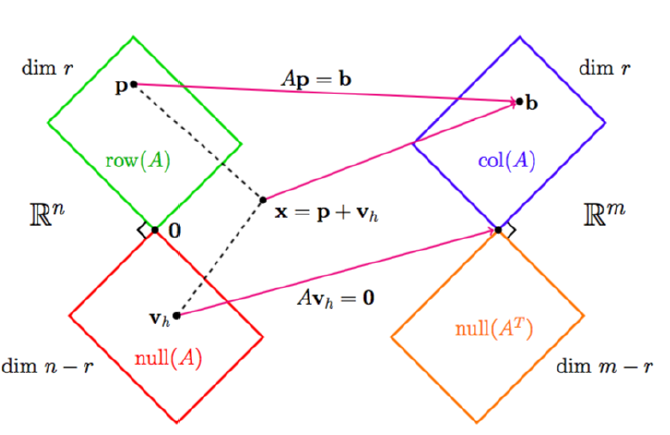
\includegraphics[scale=0.5]{Chapter4/images/ftla.png}}


%%%%%%%%%%%%%%%%%%%%%%%%%%%%Contributed by Tyler Bayn Fall 2018 %%%%%%%%%%%%%%%%%%%%%%%%%%%%%%%%%%%
%%%%%%%%%%%%%%%%%%%%%%%%%%%%%%%%%%%%%%%%%%%%%%%%%%%%%%%%%%%%%%%%%%%%%%%%%%%%%%%
\begin{center}
\begin{tikzpicture}[scale=0.75]
\node at (-4,0) {\huge $\mathbb{R}^{n}$};
\node at (4.3,0) {\huge $\mathbb{R}^{m}$};

\draw [->,>=stealth,red] (-3.3,0.2)  to [bend left]  node [above] {\large \textcolor{black}{A}}(3.6,.2);

\draw [<-,>=stealth,blue] (-3.3,-0.2) to [bend right] node [below] {\large \textcolor{black}{A$^{T}$}} (3.6,-0.2);

\end{tikzpicture}

%\hfill \break
%\hfill \break
%\hfill \break

\begin{tikzpicture}[scale=0.75]
\draw (-4.8,2.2) -- (-3.2,3.8);
\draw (-2.8,3.8) -- (-1.2,2.2);
\draw (-4.8,1.8) -- (-3.2,0.2);
\draw (-2.8,0.2) -- (-1.2,1.8);

\draw (-4.8,-2.2) -- (-3.2,-3.8);
\draw (-2.8,-3.8) -- (-1.2,-2.2);
\draw (-4.8,-1.8) -- (-3.2,-0.2);
\draw (-2.8,-0.2) -- (-1.2,-1.8);

\draw (4.8,2.2) -- (3.2,3.8);
\draw (2.8,3.8) -- (1.2,2.2);
\draw (4.8,1.8) -- (3.2,0.2);
\draw (2.8,0.2) -- (1.2,1.8);

\draw (4.8,-2.2) -- (3.2,-3.8);
\draw (2.8,-3.8) -- (1.2,-2.2);
\draw (4.8,-1.8) -- (3.2,-0.2);
\draw (2.8,-0.2) -- (1.2,-1.8);

\draw [->,>=stealth,red] (-0.8,2.3) -- node [above] {\large \textcolor{black}{A}} (0.8,2.3);

\draw [<-,>=stealth,blue] (-0.8,1.7) -- node [below] {\large \textcolor{black}{A$^{T}$}} (0.8,1.7);

\node at (-3,0) {\large0};
\node at (3,0) {\large0};

\node at (-5.3,2.05) {\large dim $r$};
\node at (-5.3,-2) {\large $n - r$};
\node at (5.3,2.05) {\large dim $r$};
\node at (5.3,-2) {\large $n - r$};

\node at (-3,2) {\LARGE im(A$^{T}$)};
\node at (3,2) {\LARGE im(A)};
\node at (-3,-2) {\LARGE ker(A)};
\node at (3,-2) {\LARGE ker(A$^{T}$)};

\draw [->,>=stealth,red] (-1,-2) -- node [above] {\large \textcolor{black}{A}} (2.6,0);

\draw [->,>=stealth,blue] (1,-2) -- node [above] {\large \textcolor{black}{A$^{T}$}} (-2.6,0);

\end{tikzpicture}

\end{center}
%%%%%%%%%%%%%%%%%%%%%%%%%%%%%%%%%%%%%%%%%%%%%%%%%%%%%%%%%%%%%%%%%%%%%%%

%NEW
\begin{Exam} Solve the linear system $\begin{linear} 3x_1\ &-\ &3x_2\ &-\ &2x_3\ &=\ &3\\ -5x_1\ &+\ &4x_2\ &+\ &3x_3\ &=\ &-4\\ x_1\ &-\ &5x_2\ &-\ &2x_3\ &=\ &5 \end{linear}$ by finding the particular solution contained in the row space of the coefficient matrix.
\[\mtx{rrr|r}{3&-3&-2&3\\-5&4&3&-4\\1&-5&-2&5} \sim \mtx{rrr|r}{1&0&-1/3&0\\0&1&1/3&-1\\ 0&0&0&0}.\] Thus, the linear system is consistent and we see that 
\[\bb x = \vr{0\\-1\\0} + t\vr{1\\-1\\3},\] is the general solution to the linear system where $(1,-1,3)\in \nul(A)$. But $(0,-1,0) \notin \row(A)$. We know this since $(0,-1,0)\cdot (1,-1,3) = 1\neq 0$. On the other hand, we may solve the equation $\bb x_{\row(A)} \cdot (1,-1,3) = 0$. 
\[\bb x_{\row(A)} \cdot \vr{1\\-1\\3} =  \left(\vr{0\\-1\\0} + t\vr{1\\-1\\3}\right) \cdot \vr{1\\-1\\3} = \vr{0\\-1\\0}\cdot \vr{1\\-1\\3} + t\vr{1\\-1\\3}\cdot \vr{1\\-1\\3} = 0\]
\[(0+1+0) + t(1+1+9) = 0 \qRightarrow 1 + 11t = 0 \qRightarrow t = -\dfrac{1}{11}.\] Hence, $\bb x_{\row(A)} = \vr{0\\-1\\0} -\dfrac{1}{11}\vr{1\\-1\\3} = \vr{-1/11 \\ -10/11 \\ -3/11}$. It can be verified that $x_{\row(A)}$ is both a solution to the linear system and a member of $\row(A)$ (since it is orthogonal to $\nul(A)$).
\end{Exam}

%NEW
\begin{Exam} Solve the matrix equation $\mtx{rrrrr}{2&-6&0&0&0\\
3&-7&4&14&4\\
4&-19&-14&-49&-14\\
3&-6&6&21&6\\
-1&2&-2&-7&-2}\vr{x_1\\x_2\\x_3\\x_4\\x_5}=\mtx{c}{-72\\-78\\-249\\-63\\21}$ by finding the particular solution contained in the row space of the coefficient matrix.\\

We quickly solve the matrix equation $A\bb x=\bb b$. We do this by row reducing the augmented matrix $[A\mid \bb b]$ to RREF. We then grab the particular solution associated to setting all free variables to zero and also grab the basis to the null space of the coefficient matrix from the RREF:
\[\mtx{rrrrr|c}{2&-6&0&0&0&-72\\
3&-7&4&14&4&-78\\
4&-19&-14&-49&-14&-249\\
3&-6&6&21&6&-63\\
-1&2&-2&-7&-2&21} \sim \mtx{rrrrr|r}{1&0&6&21&6&9\\0&1&2&7&2&15\\0&0&0&0&0&0\\0&0&0&0&0&0\\0&0&0&0&0&0}.\] Hence,
\[\nul(A) = \Span\left\{\vr{-6\\-2\\1\\0\\0}, \vr{-21\\-7\\0\\1\\0}, \vr{-6\\-2\\0\\0\\1}\right\}\] and 
\[\bb x = \vr{9\\15\\0\\0\\0} + r\vr{-6\\-2\\1\\0\\0} +s \vr{-21\\-7\\0\\1\\0}+ t\vr{-6\\-2\\0\\0\\1} = \mtx{c}{9-6r-21s-6t\\15-2r-7s-2t\\r\\s\\t}.\] To find the unique solution $\bb x_{\row(A)}\in \row(A)$, we utilize the fact that $\row(A)^\top = \nul(A)$. Hence, $\bb x_{\row(A)}$ will be orthogonal to each vector in the basis of $\nul(A)$:
\begin{multline*}
\begin{linear}
\bb x_{\row(A)}\cdot (-6,-2,1,0,0)\ &= \ &0\\
\bb x_{\row(A)}\cdot (-21,-7,0,1,0)\ &=\ &0\\
\bb x_{\row(A)}\cdot (-6,-2,0,0,1)\ &= \  &0
\end{linear}\sim \begin{linear}
 -6(9-6r-21s-6t)-2(15-2r-7s-2t)+r\ &=\ &0\\
 -21(9-6r-21s-6t)-7(15-2r-7s-2t)+s\ &=\ &0\\
 -6(9-6r-21s-6t)-2(15-2r-7s-2t)+t\ &=\ &0
\end{linear}\\
\sim \begin{linear}
41r\ &+\ &140s\ &+\ &40t\ &=\ &84\\
140r\ &+\ &491\ &+\ &140t\ &=\ &294\\
40r\ &+\ &140s\ &+\ &41t\ &=\ &84
\end{linear}
\end{multline*} Solving this linear system, we get
\[\mtx{ccc|c}{41&140&40&84\\140&491&140&294\\40&140&41&84} \sim \mtx{ccc|c}{1&0&0&\frac{84}{571}\\0&1&0&\frac{294}{571}\\0&0&1&\frac{84}{571}}.\] Therefore, \[\bb x_{\row(A)} = \vr{9\\15\\0\\0\\0} + \frac{84}{571}\vr{-6\\-2\\1\\0\\0} +\frac{294}{571} \vr{-21\\-7\\0\\1\\0}+ \frac{84}{571}\vr{-6\\-2\\0\\0\\1} = \dfrac{1}{571}\mtx{c}{-2043\\6171\\84\\294\\84}. \qedhere \]
\end{Exam}

%%%%%%%%%%%%%%%%%% Exercises %%%%%%%%%%%%%%%%%%%
\startExercises{fundamental}

\noindent For Exercises \ref{exer:fundmatrixparamstart}-\ref{exer:fundmatrixparamstop}, consider the matrix $A$ and the bases for two of its fundamental subspaces, e.g., $\col(A)$ and $\nul(A)$. How many rows and columns does $A$ have, that is, what parameters $m\times n$ describe $A$? 
\begin{enumerate}[!HW!, start=1]
\item\label{exer:fundmatrixparamstart} $\col(A) = \Span\left\{\vr{2\\1}, \vr{-1\\0}\right\},\quad \nul(A)=\Span\left\{\vr{1\\-2\\1\\0\\0}, \vr{-3\\4\\0\\1\\0}, \vr{-5\\0\\0\\0\\1}\right\}$ %Daven Triplett
\item $\col(A) = \Span\left\{\vr{2\\3\\0\\-2}, \vr{-2\\4\\0\\-1}, \vr{2\\-5\\6\\4}\right\},\quad \nul(A)=\Span\left\{\vr{0\\0\\0\\1}\right\}$ %Daven Triplett
\item $\row(A) = \Span\left\{\vr{1\\0\\1}, \vr{0\\1\\2}\right\},\quad \lnl(A)=\Span\left\{\vr{7\\1\\-2}\right\}$  %Daven Triplett
\item\label{exer:fundmatrixparamstop} $\row(A) = \Span\left\{\vr{1\\2}\right\},\quad \lnl(A)=\Span\left\{\mtx{c}{1\\0\\0\\-1/4}, \mtx{c}{0\\1\\0\\1/2}, \mtx{c}{0\\0\\1\\-3/4}\right\}$ %Daven Triplett
\end{enumerate}

\noindent For Exercises \ref{exer:lnlstart}-\ref{exer:lnlstop}, compute a basis for the left null space $\lnl(A)$ where $A$ is the matrix provided. Answers may vary.
\begin{enumerate}[!HW!, label=$\spadesuit$ \arabic*., ref=\arabic*]
\begin{multicols}{3}
\item\label{exer:lnlstart} $\mtx{rrr}{-3&2&1\\7&-6&-5\\-7&4&1}$ %NEW
\itemspade $\mtx{rr}{1&2\\3&4\\5&6\\7&8\\9&10}$ %NEW
\item\label{exer:lnlstop} $ \mtx{rrrrr}{2&-2&-24&-46&114\\8&-8&-26&-44&106\\-7&7&5&3&-4\\-2&2&10&18&-44}$ %NEW
\end{multicols}
\end{enumerate}

\noindent For Exercises \ref{exer:rowsolutionstart}-\ref{exer:rowsolutionstop}, solve the linear system $A\bb x=\bb b$ by finding a particular solution in the row space of the coefficient matrix, that is, find $\bb x_{\row(A)}$.
\begin{enumerate}[!HW!, label=$\spadesuit$ \arabic*., ref=\arabic*]
\begin{multicols}{2}
\item\label{exer:rowsolutionstart} $\mtx{rr}{2&3\\-4&-6}\vr{x_1\\x_2} = \vr{2\\-4}$ %NEW
\itemspade $\mtx{rrr}{1&0&-3\\-2&3&0\\-1&-2&7}\vr{x_1\\x_2\\x_3} = \vr{-8\\4\\16}$ %NEW
\end{multicols}
\item\label{exer:rowsolutionstop} $\mtx{rrrr}{6&6&1&5\\1&1&0&1\\-2&-2&-4&2\\0&0&-3&3}\vr{x_1\\x_2\\x_3\\x_4} = \vr{9\\2\\8\\9}$ %New
\end{enumerate}

%%%%%%%%%%%%%%%%%%% Footnotes %%%%%%%%%%%%%%%%%%%
 \mbox{}\vfill
 
\pagebreak%4.6 The Fundamental Theorem of Linear Algebra
\begin{center} 
\emph{``Anyone who imagines that bliss is normal is going to waste a lot of time running around shouting that he has been robbed.'' -- Jenkins Lloyd Jones}
\end{center}

\section{The Gram-Schmidt Algorithm}\label{sec:gram}
Using orthogonal projections, we can construct an orthogonal basis from a given basis. If desired, we can also construct an orthonormal basis by normalizing.\\

\begin{Thm}[The Gram-Schmidt Process]
Let $\B=\{\bb x_1, \ldots, \bb x_p\}$ be a basis for a subspace $W\le F^n$. Define recursively the vectors
\begin{eqnarray*}
\bb v_1 &=& \bb x_1\\
\bb v_2 &=& \bb x_2 - \dfrac{\bb v_1\cdot \bb x_2}{ \bb v_1\cdot \bb v_1}\bb v_1\\
\bb v_3 &=& \bb x_3 - \dfrac{\bb v_1\cdot \bb x_3}{\bb v_1\cdot \bb v_1}\bb v_1 - \dfrac{\bb v_2\cdot \bb x_3}{\bb v_2\cdot \bb v_2}\bb v_2\\
&\vdots&\\
\bb v_p &=& \bb x_p - \dfrac{\bb v_1\cdot \bb x_p}{\bb v_1\cdot \bb v_1}\bb v_1 - \ldots - \dfrac{\bb v_{p-1}\cdot \bb x_p}{\bb v_{p-1}\cdot \bb v_{p-1}}\bb v_{p-1}
\end{eqnarray*} Then $\c = \{\bb v_1, \ldots, \bb v_p\}$ is an orthogonal basis of $W$. In addition, 
\[\Span\{\bb v_1, \ldots, \bb v_k\} = \Span\{\bb x_1,\ldots, \bb x_k\}\qquad \forall k.\]
\end{Thm}\vs
%\begin{Thm}[The Gram-Schmidt Process]
%Let $\{\bb x_1, \ldots, \bb x_p\}$ be a basis for a subspace $W\le V$. Define recursively the vectors
%\begin{eqnarray*}
%\bb v_1 &=& \bb x_1\\
%\bb v_2 &=& \bb x_2 - \dfrac{\langle \bb x_2,\ \bb v_1\rangle}{\langle \bb v_1,\ \bb v_1\rangle}\bb v_1\\
%\bb v_3 &=& \bb x_3 - \dfrac{\langle\bb x_3,\ \bb v_1\rangle}{\langle\bb v_1,\ \bb v_1\rangle}\bb v_1 - \dfrac{\langle\bb x_3,\ \bb v_2\rangle}{\langle\bb v_2,\ \bb v_2\rangle}\bb v_2\\
%&\vdots&\\
%\bb v_p &=& \bb x_p - \dfrac{\langle\bb x_p,\ \bb v_1\rangle}{\langle\bb v_1,\ \bb v_1\rangle}\bb v_1 - \ldots - \dfrac{\langle\bb x_p,\ \bb v_{p-1}\rangle}{\langle\bb v_{p-1},\ \bb v_{p-1}\rangle}\bb v_{p-1}
%\end{eqnarray*} Then $\C = \{\bb v_1, \ldots, \bb v_p\}$ is an orthogonal basis of $W$. In addition, 
%\[\Span\{\bb v_1, \ldots, \bb v_k\} = \Span\{\bb x_1,\ldots, \bb x_k\}\qquad \forall k.\]
%\end{Thm}\vs
%\begin{proof}
%We shall prove the theorem by induction. Let $\B_k = \{\bb v_1, \ldots, \bb v_k\}$ and $W_k = \Span(\B_k)$. Then we mention that $\bb v_{k+1} = \bb x_{k+1} - \proj_{W_k} \bb x_{k+1}$.\\
%
%For the base case, notice that $\{\bb v_1\} = \{\bb x_1\}$ is an orthogonal basis for $W_1 = \Span\{\bb v_1\} = \Span\{\bb x_1\}$. For our induction hypothesis, suppose that $W_i = \Span\{\bb x_1, \ldots, \bb x_i\}$ and $\B_i$ is an orthogonal basis for $W_i$ for all $i < k$. \\
%
%For the inductive step, let $\widehat{\bb x_k} = \proj_{W_{k-1}} \bb x_k$. Since $\bb v_k = \bb x_k - \widehat{\bb x_k}$ and $\widehat{\bb x_k} \in W_{k-1}$, $\Span\{\bb x_1, \ldots, \bb x_{k-1}, \bb x_k\} = \Span\{\bb x_1, \ldots, \bb x_{k-1}, \bb v_k\}$. Using our inductive hypothesis, we get
%\[\Span\{\bb x_1, \ldots, \bb x_{k-1}, \bb x_k\} = \Span\{\bb x_1, \ldots, \bb x_{k-1}, \bb v_k\}  = \Span\{\bb v_1, \ldots, \bb v_{k-1}, \bb v_k\} = W_k.\] Also, by our inductive hypothesis, $\B_{k-1}$ is an orthogonal set. Since $\bb v_k = \bb x_k - \widehat{\bb x_k} \in W_{k-1}^\perp$, the set $\B_k$ is orthogonal and hence is linearly independent. Therefore, $\B_k$ is an orthogonal basis of $W_k$. In particular, when $k=p$, $\{\bb v_1, \ldots, \bb v_p\}$ is an orthogonal basis of $W$.
%\end{proof}\vs

\begin{Exam}\label{exam} Let $\bb x_1 = \vr{1\\1\\1\\1}$, $\bb x_2 = \vr{0\\1\\1\\1}$, and $\bb x_3 = \vr{0\\0\\1\\1}$, which as a set is linearly independent. Let $W = \Span\{\bb x_1, \bb x_2, \bb x_3\}$. Then using the Gram-Schmidt procedure, we can construct an orthogonal basis of $W$.
\begin{eqnarray*}
\bb v_1 &=& \bb x_1 = \vr{1\\1\\1\\1}\\
\bb v_2 &=& \bb x_2 - \dfrac{\bb v_1\cdot \bb x_2}{\bb v_1\cdot \bb v_1}\bb v_1 = \vr{0\\1\\1\\1} - \dfrac{3}{4}\vr{1\\1\\1\\1} = \vr{-3/4\\1/4\\1/4\\1/4}\\
\bb v_3 &=& \bb x_3 - \dfrac{\bb v_1\cdot \bb x_3}{\bb v_1\cdot \bb v_1}\bb v_1 - \dfrac{\bb v_2\cdot \bb x_3}{\bb v_2\cdot \bb v_2}\bb v_2 = \vr{0\\0\\1\\1} - \dfrac{2}{4}\vr{1\\1\\1\\1} - \dfrac{1/2}{12/16}\vr{-3/4\\1/4\\1/4\\1/4} \\
&=& \vr{0\\0\\1\\1} - \vr{1/2\\1/2\\1/2\\1/2} - \vr{-3/6\\1/6\\1/6\\1/6} = \vr{0\\-2/3\\1/3\\1/3}
\end{eqnarray*} Note that
\[\bb v_1\cdot \bb v_2 = -3/4+1/4+1/4+1/4=0,\quad \bb v_1\cdot \bb v_3 = 0-2/3+1/3+1/3=0,\quad \bb v_2\cdot \bb v_3 = 0-2/3+1/3+1/3 = 0.\] Therefore, $\{\bb v_1, \bb v_2, \bb v_3\}$ is an orthogonal basis for $W$. If we normalize:
\[\bb u_1 = \dfrac{1}{\sqrt{4}}\vr{1\\1\\1\\1} = \vr{1/2\\1/2\\1/2\\1/2}, \quad \bb u_2 = \sqrt{\dfrac{4}{3}}\vr{-3/4\\1/4\\1/4\\1/4} = \vr{-3/\sqrt{12}\\1/\sqrt{12}\\1/\sqrt{12}\\1/\sqrt{12}},\quad \bb u_3 = \sqrt{\dfrac{9}{6}}\vr{0\\-2/3\\1/3\\1/3} = \vr{0\\-2/\sqrt{6}\\1/\sqrt{6}\\1/\sqrt{6}},\] then
$\{\bb u_1, \bb u_2, \bb u_3\}$ is an orthonormal basis of $W$.
\end{Exam}\vs


\begin{Exam} Let $\bb u = \vr{1 \\ i \\ 0}$ and $\bb v = \vr{1 \\ 0 \\ -i}$. Let $W = \Span\{\bb u,\ \bb v\} \subseteq \C^n$. Compute an orthogonal basis for $W$. \\

The set $\{\bb u,\ \bb v\}$ is a basis for $W$ since the set is linearly independent ($\bb v \neq z\bb u$ for any scalar $z\in \C$). Applying the Gram-Schmidt process, we set $\bb x_1 = \bb u$ and 
\[\bb x_2 = \bb v - \dfrac{\bb u \cdot \bb v}{\bb u \cdot \bb u}\bb u = \vr{1 \\ 0 \\ -i} - \dfrac{1}{2}\vr{1\\ i \\ 0} = \vr{1/2 \\ -i/2 \\ -i}.\] Note that 
\[\bb x_1 \cdot \bb x_2 = 1\left(\dfrac{1}{2}\right) - i\left(-\dfrac{i}{2}\right) + 0(-i) = \dfrac{1}{2} - \dfrac{1}{2} = 0.\] Thus, $\{\bb x_1,\ \bb x_2\}$ is an orthogonal basis for $W$.
\end{Exam}\vs

\begin{Thm}[The $QR$ Factorization] If $A$ is an $m\times n$ matrix with linearly independent columns, then $A$ can be factored as $A =  QR$, where $Q$ is an $m\times n$ matrix with orthonormal columns and $\col A = \col Q$ and $R$ is an $n\times n$ upper triangular matrix with positive diagonal entries. In particular, $R$ is necessarily invertible.
\end{Thm}
%\begin{proof}
%Build $Q$ such that the columns of $Q$ are an orthonormal basis of $\col A$. Since the columns of $A$ are linearly independent, $Q$ is an $m\times n$ matrix. Let $\bb x_i$ and $\bb u_i$ be the $i$th column of $A$ and $Q$, respectively. Using the Gram-Schmidt method, we can choose the columns of $Q$ such that  \[\Span\{\bb x_1, \ldots, \bb x_k\} = \Span\{\bb u_1, \ldots, \bb u_k\}\] for all $k \le n$. In particular, there exists scalars $r_{ik}\in \R$ such that
%\begin{equation}\label{eq:o}\bb x_k = r_{1k}\bb u_1 + r_{2k}\bb u_2 + \ldots + r_{kk}\bb u_k + 0\bb u_{k+1} + \ldots + 0\bb u_n.\end{equation} Let $R = \mtx{c}{r_{ik}}$. Then the columns vectors of $R$ are of the form $\bb r_k =\mtx{c}{r_{1k} \\ \vdots \\ r_{kk} \\ 0 \\\vdots \\ 0}$. Therefore, $R$ is upper triangular. By the independence of the columns of $A$ and the construction of the orthonormal basis via the Gram-Schmidt orthogonalization, the weight $r_{kk}\neq 0$. By switching $\bb u_k$ with $-\bb u_k$, if necessary, we may assume that $r_{kk} > 0$. By \eqref{eq:o}, $\bb x_k = Q\bb r_k$. Therefore, $A = QR$.
%\end{proof}\vs

The matrix $Q$ is constructed by using an orthonormal basis provided by the Gram-Schmidt process, although some columns might need to be scaled by $-1$ to guarantee that the diagonal entries of $R$ are positive. If $A = QR$, then it can be shown that $R = \mtx{c}{\langle \bb q_i,\ \bb a_j\rangle}$, where $\bb q_i$ and $\bb a_j$ denote the columns of $Q$ and $A$, respectfully. With respect to the dot product, this gives that $Q^\top A = R$. \\

\begin{Exam} Let $A  = \mtx{ccc}{1&0&0\\1&1&0\\1&1&1\\1&1&1}$. By \examref{exam}, $\{\bb u_1, \bb u_2, \bb u_3\}$ is an orthonormal basis for $\col A$ where \[Q = \mtx{ccc}{\bb u_1 & \bb u_2 & \bb u_3} = \mtx{ccc}{1/2&-3/\sqrt{12}&0\\1/2&1/\sqrt{12}&-2/\sqrt{6}\\1/2&1/\sqrt{12}&1/\sqrt{6}\\1/2&1/\sqrt{12}&1/\sqrt{6}}.\] Let \[R = Q^\top A = \mtx{cccc}{1/2 & 1/2&1/2&1/2 \\ -3/\sqrt{12}&1/\sqrt{12}&1/\sqrt{12}&1/\sqrt{12} \\ 0&-2/\sqrt{6}&1/\sqrt{6}&1/\sqrt{6}}\mtx{ccc}{1&0&0\\1&1&0\\1&1&1\\1&1&1} = \mtx{ccc}{2 & 3/2 & 1 \\ 0 & 3/\sqrt{12} & 1/\sqrt{3} \\ 0 & 0 & 2/\sqrt{6}}.\] Therefore, $A = QR$.
\end{Exam}\vs

%%%%%%%%%%%%%%%%%% Exercises %%%%%%%%%%%%%%%%%%%
\startExercises{gram}

\noindent For Exercises \ref{exer:orthobasisstart}-\ref{exer:orthobasisstop}, apply the Gram-Schmidt algorithm to find an orthonormal basis for each subspace $W$ provided.
\begin{enumerate}[!HW!, start=1, label=$\spadesuit$ \arabic*., ref=\arabic*]
\begin{multicols}{3}
\item\label{exer:orthobasisstart} $\Span\left\{\vr{1\\1}, \vr{-1\\2}\right\}$ %Hefferon 2.11
\itemspade $\Span\left\{\vr{1\\1}, \vr{2\\1}\right\}$ %Hefferon 2.11
\itemspade $\Span\left\{\vr{3\\4}, \vr{1\\2}, \vr{2\\2}\right\}$ %Jordan Griffith
\end{multicols}
\begin{multicols}{3}
\item $\Span\left\{\vr{3\\4}, \vr{1\\2}, \vr{2\\2}\right\}$ %Jordan Griffith
\itemspade $\Span\left\{\vr{1\\0\\3\\1}, \vr{2\\1\\4\\2}\right\}$ %Malcolm Hanks
\itemspade $\Span\left\{\vr{1\\2\\3}, \vr{2\\1\\-3}, \vr{3\\3\\3}\right\}$%Hefferon 
\end{multicols}
\begin{multicols}{2}
\itemspade $\Span\left\{\mtx{c}{1\\-i\\2i}, \mtx{c}{0\\1\\1-i}\right\}$ %NEW
\item\label{exer:orthobasisstop} $\Span\left\{\mtx{c}{1\\i\\-1\\-i}, \mtx{c}{1\\2\\3\\4}, \mtx{c}{1-i\\0\\3+2i\\i}\right\}$ %NEW
\end{multicols}
\end{enumerate} 

\noindent For Exercises \ref{exer:QRstart}-\ref{exer:QRstop}, compute the $QR$-factorizations of the matrix. Note that many of the column spaces of these matrices coincide with subspaces considered in Exercises \ref{exer:orthobasisstart}-\ref{exer:orthobasisstop}.
\begin{enumerate}[!HW!, label=$\spadesuit$ \arabic*., ref=\arabic*]
\begin{multicols}{4}
\item\label{exer:QRstart} $\mtx{rr}{1&-1\\1&2}$ 
%Hefferon
\itemspade $\mtx{rr}{1&2\\1&1}$ %Hefferon
\itemspade $\mtx{rr}{0&-1\\1&3}$ %Hefferon
\itemspade $\mtx{cc}{1&2\\0&1\\3&4\\1&2}$ %Malcolm Hanks
\end{multicols}
\item\label{exer:QRstop} $\mtx{rrr}{1&2&3\\2&1&3\\3&-3&3}$ %Hefferon
\end{enumerate}

%%%%%%%%%%%%%%%%%%% Footnotes %%%%%%%%%%%%%%%%%%%
 \mbox{}\vfill
 
\pagebreak%4.7 The Gram-Scmidt Process %DIRTY Hefferon exercises
\begin{center} 
\emph{``Hypotheses are what we lack the least.'' --  Henri Poincare}
\end{center}

\section{The Least Squares Problem}\label{sec:least}
In the past, we have considered the matrix equation $A\bb x = \bb b$. We have learned how to determine if the equation has a solution and how to calculate the solution set when it is consistent. In fact, if $\bb x$ is a solution, then we can decompose \[\bb x = \bb x_{\row(A)} + \bb x_{\nul(A)}\] orthogonally. But what about when $A\bb x = \bb b$ is inconsistent? Well, the solution set is empty then, but what if we really needed it to have a solution? No manner of begging will change the fact that the matrix equation does not have a solution. For example, what if we want to find a line that is incident to all of the below points. As these points are not collinear, no such line exists. But is there a line that best fits the points, a so-called \emph{regression line}? 
\begin{center}
    \begin{tikzpicture}%Ty Bayn
\draw[ultra thick, -stealth] (-1,0) -- (8,0) node[right] {$x$};
\draw[ultra thick, -stealth] (0,-1) -- (0,8) node[above] {$y$};

\draw (1.5,3) node[above left] {\large $(x_2,y_2)$}; 
\draw[ultra thick, red,dashed] (1.5,3.2) -- (2.05,2.4);
\fill (1.5,3.2) circle (0.08);

\draw (2,1.2) node[below left] {\large $(x_1,y_1)$};
\draw[ultra thick, red,dashed] (2,1.4) -- (1.55,2.05);
\fill (2,1.4) circle (0.08);

\draw[ultra thick, red,dashed] (2.5,5.2) -- (3.63,3.55);
\fill(2.5,5.2) circle (0.08);

\draw[ultra thick, red,dashed] (3,1.4) -- (2.23,2.505);
\fill(3,1.4) circle (0.08);

\draw[ultra thick, red] (3.5,3.2) -- (3.41,3.3);
\fill(3.5,3.2) circle (0.08);

\draw[ultra thick, red,dashed] (4,4.2) -- (4.2,3.9);
\fill(4,4.2) circle (0.08);

\draw[ultra thick, red,dashed] (4.5,3.2) -- (4.1,3.8);
\fill(4.5,3.2) circle (0.08);

\draw[ultra thick, red] (5,4.7) -- (5.1,4.55);
\fill(5,4.7) circle (0.08);

\draw[ultra thick, red,dashed] (5.5,3.7) -- (5,4.45);
\fill(5.5,3.7) circle (0.08);

\draw (6,5.5) node[above left] {\large $(x_n,y_n)$}; 
\draw[ultra thick, red,dashed] (6,5.7) -- (6.25,5.3);
\fill (6,5.7) circle (0.08);

\draw [stealth-stealth,ultra thick,blue] (-1,0.3) -- (8,6.5);

\node[blue] at (9.5,7) {\large Regression Line};
\node at (9.5,6.5) {\large $y = mx + b$};

\node at (9.5,3.5) {\large
$\begin{linear}
x_1&m\ & +\ & b\ & = \ &y_1 \\
x_2&m\ & +\ & b\ & = \ &y_2 \\
x_3&m\ & +\ & b\ & = \ &y_3 \\
&&\vdots\ \\
x_n&m\ & +\ & b\ & = \ &y_n \\
\end{linear}$
};
\end{tikzpicture}
\end{center}

Instead of asking, ``Is there a vector $\bb x$ such that $A\bb x = \bb b$,'' we ask, ``Is there a vector $\bb x$ such that $A\bb x \approx \bb b$?" By approximation here, we mean to find a vector $\bb x$ such that $\Vert A\bb x - \bb b\Vert$ is sufficiently small. This leads to the \textbf{least-squares problem}. \\

\begin{Def} If $A$ is an $m\times n$ matrix and $\bb b\in F^m$, a \textbf{least-squares solution} of $A\bb x = \bb b$ is a vector $\widehat{\bb x}\in F^n$ such that 
\[\Vert \bb b - A\widehat{\bb x}\Vert \le \Vert \bb b - A\bb x\Vert\] for all $\bb x \in F^n$
\end{Def}\vs

Note that if $A\bb x = \bb b$ is consistent, then there exists a vector $\widehat{\bb x}$ such that $A\widehat{\bb x} = \bb b$ and $\Vert \bb b - A\widehat{\bb x}\Vert = \Vert \bb 0 \Vert = 0$. Thus, any solution is a least-square solution. On the other hand, if $A\bb x = \bb b$ is inconsistent, then the matrix equation has no solution but must certainly still have a least-square solution. To find this least-squares solution, let us change our focus. Why is the linear system inconsistent and who should be blamed for it? Well, the vector $\bb b$, sort of. We have also seen the $\bb b$ can be orthogonally decomposed as 
\[\bb b = \bb b_{\col(A)} + \bb b_{\lnl(A)}.\] If $A\bb x=\bb b$ is inconsistent, then it is because the left null space component of $\bb b$, that is, $\bb b_{\lnl(A)}$, is nontrivial. As we mentioned before, while the null space measures the ease of solving a consistent system (because it increases the dimension of the solution set), the left null space measures the difficulty of the system being consistent (because more rows of zeros in the echelon form of $A$ place more limitation on the choice of consistent $\bb b$).\\

Let $A$ be an $m\times n$ matrix and $\bb b\in F^m$. Let $\bb x\in F^n$ be a generic vector (treat $\bb x$ as a variable vector). Then $A\bb x$ is a generic vector of the subspace $\col A$.  Let $\widehat{\bb b} = \proj_{\col A}\bb b = \bb b_{\col(A)}$. Then 
\[\Vert \bb b - \widehat{\bb b}\Vert \le \Vert \bb b - A\bb x\Vert\] by the \hyperref[thm:bestapprox]{Best Approximation Theorem}. Since $\widehat{\bb b}\in \col A$, there exists some vector $\widehat{\bb x}\in F^n$ such that $A\widehat{\bb x} = \widehat{\bb b}$. Therefore, every linear system has a least-squares solution $\widehat{\bb x}$, which is a solution to the linear system $A\bb x = \widehat{\bb b}$, since for all $\bb x$ we have \[\Vert \bb b - A\widehat{\bb x}\Vert \le \Vert \bb b - A\bb x\Vert.\] Of course, we also have that the linear system $A\bb x = \widehat{\bb b}$ is ALWAYS consistent.\\

If $\widehat{\bb x}$ is a least-squares solution of $A\bb x = \bb b$, then $\bb b - A\widehat{\bb x} = \bb b - \widehat{\bb b} \in (\col A)^\perp = \lnl( A)$. Hence, $\bb b - A\widehat{x} = \bb b_{\lnl(A)}$. Thus, $A^\top(\bb b - A\widehat{\bb x}) = \bb 0$. Therefore, $A^\top A\widehat{\bb x} = A^\top\bb b$. In particular, every least-squares solution to $A\bb x = \bb b$ is a solution to the system of \textbf{normal equations}
\begin{equation} A^\top A\widehat{\bb x} = A^\top\bb b.\end{equation} Essentially, multiplying by $A^\top$ kills off the left null space component of $\bb b$, leaving the column space component behind. For complex linear systems, replace $^\top$ with $^*$, per the usual.\\

\begin{Thm} The set of least-squares solutions of $A\bb x = \bb b$ coincides with the solution set of the normal equations $A^\top A\widehat{\bb x} = A^\top\bb b$.\end{Thm}\vs


\begin{Exam}\label{exam:least1} Find a least-squares solution of the inconsistent system $A\bb x = \bb b$ with \\
$A = \mtx{rr}{4&0\\0&2\\1&1}$ and $\bb b = \vr{2\\0\\11}$.\\

We begin by constructing the normal equations:
\[A^\top A = \mtx{rrrr}{4&0&1\\0&2&1}\mtx{rr}{4&0\\0&2\\1&1} = \mtx{rr}{17&1\\1&5};\qquad A^\top\bb b = \mtx{rrrr}{4&0&1\\0&2&1}\vr{2\\0\\11} = \vr{19\\11}.\] Thus, $A^\top A\widehat{\bb x} = A^\top\bb b$ becomes
\[\mtx{rr}{17&1\\1&5}\bb x = \vr{19\\11}.\] Since $A^\top A$ is invertible, we have
\[\widehat{\bb x} = (A^\top A)^{-1}A^\top\bb b = \dfrac{1}{84}\mtx{rr}{5&-1\\-1&17}\vr{19\\11} = \dfrac{1}{84}\vr{84\\168} = \vr{1\\2}. \qedhere\]
\end{Exam}\vs

\begin{Exam} Find a least-squares solution for\\
$A = \mtx{rrrr}{1&1&0&0\\1&1&0&0\\1&0&1&0\\1&0&1&0\\1&0&0&1\\1&0&0&1}$ and $\bb b = \vr{-3\\-1\\0\\2\\5\\1}$.\\

\[A^\top A = \mtx{rrrr}{6&2&2&2\\2&2&0&0\\2&0&2&0\\2&0&0&2};\qquad A^\top\bb b = \vr{4\\-4\\2\\6};\qquad \mtx{rrrr|r}{6&2&2&2&4\\2&2&0&0&-4\\2&0&2&0&2\\2&0&0&2&6} \sim \mtx{rrrr|r}{1&0&0& 1&3\\0&1&0&-1&-5\\0&0&1&-1&-2\\0&0&0&0&0}.\] Therefore, 
\[\widehat{\bb x} = \vr{3\\-5\\-2\\0} + x_4\vr{-1\\1\\1\\1}. \qedhere\]
\end{Exam}

As illustrated in the last example, a least-squares solution need not be unique.\\

\begin{Thm}\label{thm:leastsquaresolution} Let $A$ be an $m\times n$ matrix. Then the following are equivalent:
\begin{enumerate}[!THM!, start=1]
\item The equation $A\bb x = \bb b$ has a unique least-squares solution for each $\bb b \in F^m$.
\item The columns of $A$ are linearly independent.
\item The matrix $A^\top A$ is invertible.
\end{enumerate} In this situation, the unique least-squares solution has the form
\[\widehat{\bb x } = (A^\top A)^{-1}A^\top\bb b.\]
\end{Thm}

\begin{Exam} The matrix $A$ given in \examref{exam:least1} has a unique least-squares solution for all $\bb b \in \R^m$. \end{Exam}\vs

Least-squares solutions also allow us to compute orthogonal projections without an orthogonal basis. For example, if $W = \Span\{\bb v_1, \ldots, \bb v_r\} \le F^n$,  $A = \mtx{cccc}{\bb v_1 & \bb v_2 & \ldots & \bb v_r}$, and $\bb y \in F^n$, then $W = \col(A)$ and $\widehat{\bb y} = \proj_W(\bb y) = \proj_{\col(A)}(\bb y) = \bb y_{\col(A)} = A\widehat{\bb x}$ where $\bb x$ is a least-squares solutions to $A\bb x = \bb y$.\\

\begin{Exam}\label{exam:proj} Let $W = \col(A)$, where $A$ is defined in \examref{exam:least1}. Then $\widehat{\bb b} = \proj_W(\bb b) = A\widehat{\bb x} = \mtx{rr}{4&0\\0&2\\1&1}\vr{1\\2} = \vr{4\\4\\3}$. Thus, we may find  orthogonal projections by solving least-squares problem.
\end{Exam}

In the vein of the previous example, the standard matrix of the orthogonal projection from $F^n$ onto the subspace $W$ is $A(A^\top A)^{-1}A^\top$, where the columns of $A$ correspond to a basis for $W$, since $\bb b  \mapsto A(A^\top A)^{-1}A^\top \bb b = A\widehat{\bb x} = \widehat{b} = \proj_W(\bb b)$. Of course, if $A=QR$ is a $QR$ factorization, then 
\[A(A^\top A)^{-1}A^\top = QR((QR)^\top QR)^{-1}(QR)^\top = QR(R^\top Q^\top QR)^{-1}R^\top Q^\top = QR(R^\top R)^{-1}R^\top Q^\top = QR(R^{-1}(R^\top)^{-1})R^\top Q^\top = QQ^\top.\] This second form appears much simpler (and agrees with the formula we found in \secref{sec:orthoproj}), but this is because know $A=QR$ means we have an orthonormal basis for $W$, namely the columns of $Q$. The advantage of $A(A\top A)^{-1}A^\top$ is that no orthogonalization is necessarily to determine $\proj_W$.

\begin{Exam} Let $A = \mtx{rr}{4&0\\0&2\\1&1}$ and $W=\col(A)$. Let $T : \R^3\to \R^3$ be the orthogonal projection onto $W$. Then 
\[[T] =A(A^\top A)^{-1}A^\top  = \mtx{rr}{4&0\\0&2\\1&1}\mtx{rr}{17&1\\1&5}^{-1} \mtx{rrrr}{4&0&1\\0&2&1} = \dfrac{1}{84}\mtx{rr}{4&0\\0&2\\1&1} \mtx{rr}{5&-1\\-1&17} \mtx{rrrr}{4&0&1\\0&2&1} \]
\[=\dfrac{1}{84}\mtx{rr}{20 &-4 \\ -2 & 34 \\ 4 & 16}\mtx{rrrr}{4&0&1\\0&2&1}= \dfrac{1}{84}\mtx{rrr}{80 & -8 & 16 \\ -8 & 68 & 32 \\ 16 & 32 & 20} = \dfrac{1}{21}\mtx{rrr}{20 & -2 & 4 \\ -2 & 17 & 8 \\ 4 & 8 & 5} \]

Note that 
\[\dfrac{1}{21}\mtx{rrr}{20 & -2 & 4 \\ -2 & 17 & 8 \\ 4 & 8 & 5}\vr{2\\0\\11} = \dfrac{1}{21}\vr{40+0+44 \\ -4 + 0 +88 \\ 8+0+55} = \dfrac{1}{21}\vr{84 \\ 84 \\ 63} = \vr{4\\4\\3}. \qedhere\]
\end{Exam}\vs

\begin{Thm} Let $A$ be an $m\times n$ matrix with linearly independent columns. Let $A = QR$ be a $QR$ factorization. Let $\bb b\in F^m$. Then the unique least-squares solution $\widehat{\bb x}\in F^n$ has the form
\[\widehat{\bb x} = R^{-1}Q^\top \bb b.\]
\end{Thm}
\begin{proof}
Let $\widehat{\bb x} = R^{-1}Q^\top \bb b$. Then 
\[A\widehat{\bb x} = A(R^{-1}Q^\top \bb b) = QR(R^{-1}Q^\top \bb b) = QQ^\top  \bb b = \proj_{\col Q} \bb b,\] since $QQ^\top$ is the standard matrix representation for $\proj_{\col Q}$. Since $\col Q = \col A$, $\widehat{\bb x}$ is a least-squares solution of $A\bb x = \bb b$. By \thmref{thm:leastsquaresolution}, this is the unique least-squares solution.
\end{proof}

%%%%%%%%%%%%%%%%%% Exercises %%%%%%%%%%%%%%%%%%%
\startExercises{least}

\noindent For Exercises \ref{exer:leaststart}-\ref{exer:leaststop}, compute the least square solutions for linear system.
\begin{enumerate}[!HW!, start=1, label=$\spadesuit$ \arabic*., ref=\arabic*]
\begin{multicols}{3}
\item\label{exer:leaststart} $\mtx{rr|r}{1 & -1 & 2\\ 2 & 3 & -1\\ 4 & 5 & 5}$ %Anton 6.4.3 p. 386
\itemspade $\mtx{rr|r}{9&1&-27\\1&0&13\\2&-1&1\\1&0&0}$ %NEW
\item\label{exer:leaststop} $\mtx{rrr|r}{2&0&-1&0\\1&-2&2&6\\2&-1&0&0\\0&1&-1&6}$ %Anton 6.4.6 p. 386
\end{multicols}
\end{enumerate}

\noindent For Exercises \ref{exer:leastorthoprojstart}-\ref{exer:leastorthoprojstop}, compute the orthogonal projection $\proj_W(\bb b)$ using the method of least squares as in \examref{exam:proj} where $W = \col(A)$, where $A$ is the matrix provided first and $\bb b$ is the vector provided second.
\begin{enumerate}[!HW!, label=$\spadesuit$ \arabic*., ref=\arabic*]
\begin{multicols}{2}
\item\label{exer:leastorthoprojstart} $\mtx{rr}{1&-1\\3&2\\-2&4}$, $\vr{4\\1\\3}$ %Anton 6.4.15 p. 386
\item\label{exer:leastorthoprojstop} $\mtx{rr}{5&1\\1&3\\4&-2}$, $\vr{-4\\2\\3}$ %Anton 6.4.16 p. 386
\end{multicols}
\end{enumerate}

\noindent For Exercises \ref{exer:leastorthostart}-\ref{exer:leastorthostop},  compute the orthogonal projection $\proj_W(\bb b)$ using the method of least-squares. where a basis for $W$ is provided first and the vector $\bb b$ is the vector provided second.
\begin{enumerate}[!HW!, label=$\spadesuit$ \arabic*., ref=\arabic*]
\begin{multicols}{2}
\item\label{exer:leastorthostart} $\left\{(-1,2,1),\ (2,2,4)\right\},\ (1, -6, 1)$ %Anton 6.4.17 p. 386
\item\label{exer:leastorthostop} $\left\{(2,1,1,1),\ (1,0,1,1),\ (-2,-1,0,-1)\right\},\ (6,3,9,6)$ %Anton 6.4.18 p. 386
\end{multicols}
\end{enumerate}\vs

\noindent For Exercises \ref{exer:leastbasisprojstart}-\ref{exer:leastbasisprojstop}, find a basis for $W$ and the standard matrix for the orthogonal projection onto $W$. Answers may vary.
\begin{enumerate}[!HW!, label=$\spadesuit$ \arabic*., ref=\arabic*]
\item\label{exer:leastbasisprojstart} $W$ is the plane given by the equation $5x-3y+z=0$ in $\R^3$. %Anton 6.4.25 p. 386
\item\label{exer:leastbasisprojstop} $W$ is the line with parametric equations $x=2t$, $y=-t$, and $z=4t$ in $\R^3$.\\ %Anton 6.4.26 p. 387
\end{enumerate}

\begin{enumerate}[!HW!]
\item If $A$ is a nonsingular matrix, show that the unique least squares solution $\widehat{\bb x}$ to the linear system $A\bb x = \bb b$ is likewise the unique linear solution to $A\bb x = \bb b$. %Jacob Jensen

\item Suppose that $A = QR$ is a $QR$ factorization of $A$. If $A\bb x = \bb b$ has a unique least-squares solution, show that $\widehat{x} = R^{-1}Q^\top \bb b$ is this solution. 
\end{enumerate}

%%%%%%%%%%%%%%%%%%% Footnotes %%%%%%%%%%%%%%%%%%%
 \mbox{}\vfill
 
\pagebreak%4.8 Least Squares Problem %DIRTY EXERCISES

%%%% Chapter 5 %%%%%%
\chapter{Determinants}\label{chap:deter}

\pagebreak%Determinants
\begin{center} 
\emph{``Our lives will depend upon the decisions which we make--for decisions determine destiny.'' \\-- Thomas S. Monson}
\end{center}

\section{Introduction to Determinants}\label{sec:deter}
In a previous section, we discussed the inverse of a $2\times 2$ matrix $A = \mtx{cc}{a&b\\c&d}$:
\[A^{-1} = \dfrac{1}{ad-bc}\mtx{rr}{d&-b\\-c&a}.\] The quantity $ad-bc$ was called the \textbf{determinant} of $A$, denoted $\det A$ or $|A|$. In this chapter we work to generalize this idea for any square matrix. Our strategy will be to define determinants recursively. We will remind the reader that, unlike the previous chapter, the theory of determinants is applicable to any field. Hence, $F$ will denote an arbitrary field. \\

\begin{Def} Let $A$ be an $n\times n$ matrix. Define the $(i,j)$-\textbf{minor matrix} $A_{ij}$ to be the $(n-1)\times (n-1)$ matrix which results by removing the $i$th row and $j$th column from $A$.
\end{Def}\vs

%%Contributed by Laura Lee Fall 2018
%\begin{Exam} Let $A = \mtx{rrr}{5 & 7 & 12 \\ 0 & 3 & 4 \\ 9 & -1 & -6}$. Compute the $(1,1)-,$ $(1,2)-$, $(2,2)-$, and $(3,3)$-minor matrix.\\
%
%\[A_{11} = \mtx{rr}{3 & 4 \\ -1 & -6}, \quad A_{12} = \mtx{rr}{0 & 4 \\ 9 & -6 }, \quad A_{22} = \mtx{rr}{5 & 12 \\ 9 & -6}, \quad A_{23} = \mtx{rr}{5 & 7 \\ 9 & -1 \\},  \quad A_{33} = \mtx{rr}{5 & 7 \\  0 & 3}. \qedhere\]
%\end{Exam}\vs

\begin{Exam} Let $A = \mtx{rrr}{1&5&0\\2&4&-1\\0&-2&0}$. Compute the $(1,1)-,$ $(1,2)-$, $(2,2)-$, and $(3,3)$-minor matrix.\\

\[A_{11} = \mtx{rr}{4&-1\\-2&0}, \quad A_{12} = \mtx{rr}{2&-1\\0&0},\quad A_{22} = \mtx{rr}{1&0\\0&0}, \quad A_{33} = \mtx{rr}{1&5\\2&4}. \qedhere\]
\end{Exam}\vs

\begin{Def} Let $A = \mtx{c}{a_{ij}}$ be an $n\times n$ matrix. For $n=1$, $A = \mtx{c}{r}$ for some $r\in F$. In this case, we define $\det A = r$. For $n > 1$, let 
\begin{eqnarray*}
\det A &=& a_{11}\det A_{11} - a_{12}\det A_{12} + \ldots + (-1)^{1+n}a_{1n}\det A_{1n}\\
&=& \sum_{j=1}^n (-1)^{1+j}a_{ij}\det A_{ij}
\end{eqnarray*} The quantity $\det A$ is called the \textbf{determinant} of $A$.
\end{Def}\vs

Let $A = \mtx{cc}{a&b\\c&d}$. Then $\det A = \dtx{cc}{a&b\\c&d} = a \det A_{11} - b \det A_{12} = a\dtx{c}{d} - b\dtx{c}{c} = ad-bc,$ which agrees with our $2\times 2$ determinant from before.\\

%%Contributed by Laura Lee Fall 2018
%\begin{Exam} Compute $\det A$ for $A = \mtx{rrr}{5 & 7 & 12 \\ 0 & 3 & 4 \\ 9 & -1 & -6}$.\\
%
%\begin{eqnarray*}
%\det A &=& \dtx{rrr}{5 & 7 & 12 \\ 0 & 3 & 4 \\ 9 & -1 & -6} = 5\dtx{rr}{3 & 4 \\ -1 & -6} - 7\dtx{rr}{0 & 4 \\ 9 & -6 } + 12\dtx{rr}{0&3\\9&-1}\\
%&=& 5(3\cdot (-6) - 4\cdot(-1)) -7(0\cdot (-6) - 4\cdot 9) + 12(0\cdot (-1) - 3\cdot 9) = 5(-14) -7(-36) +12(-27)\\
%& =& -70-252-324 = \fbox{$646$}. \qedhere
%\end{eqnarray*}
%\end{Exam}\vs

\begin{Exam} Compute $\det A$ for $A = \mtx{rrr}{1&5&0\\2&4&-1\\0&-2&0}$.\\

\begin{eqnarray*}
\det A &=& \dtx{rrr}{1&5&0\\2&4&-1\\0&-2&0} = 1\dtx{rr}{4&-1\\-2&0} - 5\dtx{rr}{2&-1\\0&0} + 0\dtx{rr}{2&4\\0&-2}\\
&=& 1(4\cdot 0 - (-1)\cdot(-2)) -5(2\cdot 0 - (-1)\cdot 0) + 0 = (0-2) - 5(0) = -2. \qedhere
\end{eqnarray*}
\end{Exam}\vs

\begin{Def}  Let $A$ be an $n\times n$ matrix. Define the $(i,j)$-\textbf{cofactor} $C_{ij}$ as 
\[C_{ij} = (-1)^{i+j}\det A_{ij}.\]
\end{Def}\vs

With this notation, 
\[\det A = a_{11}C_{11} + a_{12}C_{12} + \ldots + a_{1n}C_{1n}.\]\vs

The following diagram may help you remember the plus or minus sign in the cofactors:
\[\mtx{rrrr}{+ & -& + & \cdots \\ - & + & -&  \\ + & -& + &  \\ \vdots & & &\ddots}\]\vs

\begin{Thm}[Laplace Expansion] The determinant of an $n\times n$ matrix $A = \mtx{c}{a_{ij}}$ can be computed by a cofactor expansion across any row or down any column. The cofactor expansion across the $i$th row is 
\[\det A = a_{i1}C_{i1} + a_{i2}C_{i2} + \ldots + a_{in}C_{in} = \sum_{j=1}^n a_{ij}C_{ij}.\] The cofactor expansion down the $j$th column is
\[\det A = a_{ij}C_{1j} + a_{2j}C_{2j} + \ldots + a_{nj}C_{nj} = \sum_{i=1}^n a_{ij}C_{ij}.\]
\end{Thm}\vs

\begin{Exam} Use the cofactor expansion across the third row to compute $\det A$, where $A = \mtx{rrr}{1&5&0\\2&4&-1\\0&-2&0}$.

\begin{eqnarray*}
\det A &=& \dtx{rrr}{1&5&0\\2&4&-1\\0&-2&0} = 0\dtx{rr}{5&0\\4&-1} - (-2)\dtx{rr}{1&0\\2&-1} + 0\dtx{rr}{1&5\\2&4}\\
&=& 2\dtx{rr}{1&0\\2&-1} = 2(-1-0) = \fbox{$-2$}.
\end{eqnarray*}
\end{Exam}

\begin{Exam} Compute $\det A$, where $A = \mtx{rrrrr}{3&-7&8&9&-6\\0&2&-5&7&3\\0&0&1&5&0\\0&0&2&4&-1\\0&0&0&-2&0}$.\\

We will expand across the leftmost column to maximize the number of zero coefficients.
\begin{eqnarray*}
\dtx{rrrrr}{3&-7&8&9&-6\\0&2&-5&7&3\\0&0&1&5&0\\0&0&2&4&-1\\0&0&0&-2&0} &=& 3\dtx{rrrr}{2&-5&7&3\\0&1&5&0\\0&2&4&-1\\0&0&-2&0} = 6\dtx{rrr}{1&5&0\\2&4&-1\\0&-2&0}\\
&=& 6\left(\dtx{rr}{4&-1\\-2&0} - 2\dtx{rrrr}{5&0\\-2&0}\right)=6(-2+0) = \fbox{$-12$}
\end{eqnarray*}
\end{Exam}

The matrix in the last example is nearly triangular. The method in that example is easily adapted to prove the following.\\

\begin{Thm} If $A$ is a triangular $n\times n$ matrix, then $\det A$ is the product of the entries on the main diagonal.
\end{Thm}

\begin{multicols}{2}
\begin{Thm} If $A$ is a $2\times 2$ matrix over $\R$ or $\C$, the area of the parallelogram determined by the columns of $A$ is $|\det A|$. If $A$ is $3\times 3$, the volume of the parallelepiped determined by the columns of $A$ is $|\det A|$. The higher dimensional analogues also hold.
\end{Thm}
\begin{center}
\begin{tikzpicture}
\fill[cyan!50!white] (0,0) -- (1,2) -- (4,3) -- (3,1) -- cycle;
\draw[dashed, ultra thick, gray] (1,2) -- (4,3) node[midway, above left] {$\bb v$};
\draw[dashed, ultra thick, gray] (3,1) -- (4,3) node[midway, below right] {$\bb u$}; 
\draw[->, ultra thick] (0,0) -- (3,1) node[midway, below right] {$\bb v$};
\draw[->, ultra thick] (0,0) -- (1,2) node[midway, above left] {$\bb u$};
%\draw[->, ultra thick, red] (0,0) -- (4,3) node[midway, above, yshift = -5] {\rotatebox{35}{$\bb u + \bb v$}};
\end{tikzpicture}
\end{center}
\end{multicols}\vs
%\begin{proof}
%We will prove the statement for the general case of $n\times n$. If $\det A = 0$, then the column vectors are linearly dependent and the hyper-parallelepiped spanned by them is one dimension too small. Thus, the hyper-volume is also zero. If $\det A \neq 0$, then the column vectors are linearly independent and hence span all dimensions. This hyper-parallelepiped can be sheared into a rectangular hyper-prism, that is, all angles are right. A shearing matrix $S$ is unit triangular matrices and hence have determinant equal to 1. Likewise, by permuting rows, the matrix corresponding to the rectangular hyper-prism can be transformed into a diagonal matrix $D$ by multiplying by the associated permutation matrix $P$. Then $|\det(D)| = |\det(A)| $, which is the absolute value  product of the diagonal entries. On the other hand, the hyper-volume of a hyper-prism is the product of all the lengths, which are the absolute values of the diagonal entries of $D$.
%\end{proof}\vs

\begin{Exam} Calculate the area of the parallelogram determined by the points $(-2,-2)$, $(0,3)$, $(4,-1)$, and $(6,4)$.\\

We begin by translating the parallelogram such that $(-2,-2)$ is moved to the origin. This translation does not affect the area. We now consider the parallelogram with vertices $(0,0)$, $(2,5)$, $(6,1)$, and $(8,6)$. Note that this parallelogram is the one spanned by $(2,5)$ and $(6,1)$. Therefore, 
\[\text{Area} = \text{abs}\dtx{rr}{2&6\\5&1}= |2-30| = \fbox{$28$}.\qedhere\]
\end{Exam}\vs

%\section{Properties of Determinants}
%\begin{Thm}\label{product} If $A$ and $B$ are $n \times n$ matrices, then $\det(AB) = \det(A)\det(B)$.\end{Thm}\vs
%
%\begin{Exam} Let $A = \mtx{rr}{6&1\\3&2}$ and $B =\mtx{rr}{4&3\\1&2}$. Then $\det A = 6(2)-1(3) = 9$ and $\det B = 4(2)-3(1)=5$. Thus, $\det(A)\det(B) = \fbox{$45$}$. On the other hand, 
%\[AB = \mtx{rr}{6&1\\3&2}\mtx{rr}{4&3\\1&2} = \mtx{rr}{25 & 20\\ 14&13}.\] Thus, $\det(AB) = 25(13)-20(14) = 325-280= \fbox{$45$}$. 
%\end{Exam}\vs
%
%%%%%%%%%%%%%%%%%% Exercises %%%%%%%%%%%%%%%%%%%
\startExercises{deter}
\noindent For Exercises \ref{exer:minorstart}-\ref{exer:minorstop}, for the matrix $A = \mtx{rrr}{ 5 & 7 & 12 \\ 0 & 3 & 4 \\  9 & -1 & -6}$, find the given minor.
\begin{enumerate}[!HW!, start=1]
\begin{multicols}{5}
\item\label{exer:minorstart} $A_{22}$ %Laura Lee
\item $A_{33}$ %Laura Lee
\item $A_{11}$ %Laura Lee
\item $A_{23}$ %Laura Lee
\item\label{exer:minorstop} $A_{12}$ %Laura Lee
\end{multicols}
\end{enumerate}

\noindent For Exercises \ref{exer:minorspadestart}-\ref{exer:minorspadestop}, for the matrix $B = \mtx{rrrr}{1 & 2 & 3 & 4 \\ 0 & -2 & -1 & 3 \\ 1 & 1 & 3 & 6\\ 7 & -4 & 8 & 0}$, find the given minor.
\begin{enumerate}[!HW!, label=$\spadesuit$ \arabic*., ref=\arabic*]
\begin{multicols}{5}
\item\label{exer:minorspadestart} $B_{11}$
\item $B_{13}$
\item $B_{31}$
\item $B_{33}$
\item\label{exer:minorspadestop} $B_{34}$
\end{multicols}
\end{enumerate}

%NEW
\noindent For Exercises \ref{exer:minorboringstart}-\ref{exer:minorboringstop}, for the matrix $C = \mtx{rrrr}{1&2&3&4\\0&5&3&-1\\-2&4&0&-4\\-1&3&2&5}$, find the given minor.
\begin{enumerate}[!HW!]
\begin{multicols}{3}
\item\label{exer:minorboringstart} $C_{22}$
\item $C_{23}$
\item\label{exer:minorboringstop} $C_{42}$
\end{multicols}
\end{enumerate}

\noindent For Exercises \ref{exer:minorcomplexstart}-\ref{exer:minorcomplexstop}, for the matrix $D = \mtx{cccc}{i&3i-2&2+5i&7-i\\3+i&4&7i-5&9-3i\\2+3i&5i-1&1+9i&4+5i\\7+2i&i-3&2+4i&1+2i}$, find the given minor.
\begin{enumerate}[!HW!]
\begin{multicols}{3}
\item\label{exer:minorcomplexstart} $D_{24}$%Malcolm Hanks
\item $D_{33}$%Malcolm Hanks
\item\label{exer:minorcomplexstop} $D_{14}$%Malcolm Hanks
\end{multicols}
\end{enumerate}

\noindent For Exercises \ref{exer:determinantstart}-\ref{exer:determinantstop}, compute the determinant of the matrix.
\begin{enumerate}[!HW!, label=$\spadesuit$ \arabic*., ref=\arabic*]
\begin{multicols}{3}
\item\label{exer:determinantstart} $\dtx{rr}{1 & 2 \\ 3 & 4}$
\itemspade $\dtx{cc}{i & 1+i \\ 2-i & 3-4i}$
\itemspade \mbox{$\dtx{rr}{3 & 2\\ 1 & 5} \pmod 7$}  
\end{multicols}
\end{enumerate}
\begin{enumerate}[!HW!]
\begin{multicols}{3}
\itemspade $\dtx{rrr}{1 & 2 & -1 \\ -1 & 0 & 2\\ 3 & 5 & 1}$ 
\itemspade $\dtx{rrr}{1 & 2 & 3\\ 3 & -2 & 5 \\ 0 & 0 & 2}$ 
\itemspade \mbox{$\dtx{rrr}{2 & 0 & 0\\ 3 & 1 & 0\\ 4 & 3 & 4} \pmod 5$} 
\end{multicols}\pagebreak
\begin{multicols}{3}
\itemspade \mbox{$\dtx{rrrr}{1 & 1 & 2 & 4 \\ 0 & 1 & 1 & 3 \\ 0 & 0 & 2 & 4 \\ 1 & 2  & 3 & 4} \pmod 5$}
\itemspade \mbox{$\dtx{rrrrr}{1 & 0 & 0 & 0 &0 \\ 0 & 0 & 0 & 1 &0 \\ 0 &0 & 1 & 0 & 0 \\ 0 &0 & 1 & 0 & 0 \\ 0 &0 & 0 &0 &1} \pmod 2$}
\item\label{exer:determinantstop} $\dtx{rrrr}{5&4&4&2\\2&4&6&8\\0&1&2&3\\3&3&3&9}$ %Shelby Bartlett
\end{multicols}
\end{enumerate}

\begin{enumerate}[!HW!]
    \item Compute $\det(A)(\bb u\cdot \bb v)$ if:
    \[A = \mtx{cc}{\pi^2&e\\5&\sqrt{\pi}},\quad \bb u = \mtx{c}{5e^3\\1\\\pi},\quad \bb v = \mtx{c}{e^{-2}\\0\\\sqrt{\pi^3}}.\] %Da Huo
\end{enumerate}

\noindent For Exercises \ref{exer:detervolumestart}-\ref{exer:detervolumestop}, compute the area, volume, or hyper-volume of the parallelogram, parallelepiped, or hyper-parallelepiped spanned by the given set of vectors. 
\begin{enumerate}[!HW!, label=$\spadesuit$ \arabic*., ref=\arabic*]
\begin{multicols}{3}
\item\label{exer:detervolumestart} $\left\{\vr{1 \\ 2}, \vr{3\\2}\right\}$ 
\itemspade $\left\{\vr{1 \\ 2 \\ 3}, \vr{4\\8\\2}, \vr{-2 \\ 3 \\ 7}\right\}$
\item\label{exer:detervolumestop} $\left\{\vr{1 \\ 2 \\ 3 \\ 4}, \vr{1 \\ 0 \\ 0 \\ 2}, \vr{0 \\ 0 \\ 1 \\-2}, \vr{2\\-3\\4\\5}\right\}$
\end{multicols}
\end{enumerate}


%%%%%%%%%%%%%%%%%%% Footnotes %%%%%%%%%%%%%%%%%%%
 \mbox{}\vfill
 
\pagebreak%5.1 Determinants
\begin{center} 
\emph{``In most encounters we can determine the kind of experience we are going to have by how we respond.''\\ -- Wayne S. Peterson}
\end{center}

\section{Properties of Determinants}\label{sec:deterprop}
Let $V$ and $W$ be vector spaces over $F$. We have seen previously that linear maps $T : V \to W$ are those that preserve the linear operations, that is, $T(\bb x+\bb y) = T(\bb x)+T(\bb y)$ and $T(c\bb x) = cT(\bb x)$ for all $\bb x,\bb y\in V$ and $c\in F$. Let $V^n = \{(\bb v_1, \bb v_2,\ldots, \bb v_n)\mid \bb v_1, \bb v_2,\ldots, \bb v_n\in V\}$, that is, $V^n$ is the set of all list of $n$ vectors from $V$. This is itself a vector space with $\dim V^n = n\dim V$. When $V=F^m$, then $V^n \cong F^{m\times n}$, the space of all $m\times n$ matrices as each list in $V^n$ can be identified with the columns vectors of an $m\times n$ matrix. \\

\begin{Def} Let $V$ and $W$ be vector spaces over $F$. Let $n\in \N$. Let $B : V^n \to W$ be a function. We say that $B$ is \textbf{multilinear} if for each $i$ and choice of vector $\bb v_1, \bb v_2, \ldots, \bb v_n\in V$ the function 
\[\bb x \mapsto f(\bb v_1, \bb v_2, \ldots, \bb v_{i-1}, \bb x, \bb v_{i+1},\ldots, \bb v_n)\] is a linear transformation. In other words, a multilinear map is one which is linear in each variable. When $n=2$, we say a multilinear map is \textbf{bilinear}. Of course, if $n=1$ then a multilinear map is simply just linear.
\end{Def}\vs

\begin{Exam} The dot product $\cdot : \R^n\times \R^n \to \R$ is bilinear since for all $\bb u, \bb v, \bb w$ and $c\in \R$ it holds
\[(\bb u+\bb v)\cdot \bb w = \bb u\cdot \bb w + \bb v\cdot \bb w, (c\bb u)\cdot \bb v = c(\bb u\cdot \bb v), \bb u\cdot (\bb v+\bb w) = \bb u\cdot \bb v + \bb u\cdot \bb w, \bb u \cdot(c\bb v) = c(\bb u \cdot \bb v).\] Thus, the dot product is linear in the first and the second factor. \\

Likewise, the tensor product $\otimes : \R^n\times \R^n \to \R^{n\times n}$ is also bilinear since  for all $\bb u, \bb v, \bb w$ and $c\in \R$ it holds
\[(\bb u+\bb v)\otimes \bb w = \bb u\otimes \bb w + \bb v\otimes \bb w, (c\bb u)\otimes \bb v = c(\bb u\otimes \bb v), \bb u\otimes (\bb v+\bb w) = \bb u\otimes \bb v + \bb u\otimes \bb w, \bb u \otimes(c\bb v) = c(\bb u \otimes \bb v). \qedhere\]
\end{Exam}\vs

Deteriminants are NOT linear transformations ($\det(A+B) \neq \det(A) +\det(B)$). The determinant map $\det  : F^{n\times n} \to F$ is multilinear with respect to both its rows and columns since $\det(A) = \det(A^\top )$. In particular, if $A$, $B$, and $C$ are $n\times n$ matrices that differ only in a single row, say the $r$th row, and assume the $r$th row of $C$ is obtained by adding corresponding entries in the $r$th rows of $A$ and $B$. Then 
\[\det(C) = \det(A) + \det(B).\] Likewise, if $A$ and $B$ are matrices that differ only in a single row, say the $r$th row, and assume the $r$th row of $B$ is obtained by scaling the  corresponding entries in the $r$th row of $A$ by $c\in F$. Then $\det(B) = c\det(A)$.\\

\begin{Exam} Note that 
\[\dtx{ccc}{  4&5&0\\3&-1&2\\ 1+0&2+4&3-2} = \dtx{rrr}{ 4&5&0\\3&-1&2\\ 1&2&3} + \dtx{rrr}{  4&5&0\\3&-1&2\\ 0&4&-2}\quad\text{and}\quad \dtx{ccc}{1&2&3\\4&6&8\\0&1&3} =  2\dtx{ccc}{1&2&3\\2&3&4\\0&1&3}. \qedhere\] %NEW
\end{Exam}\vs

The following is probably the most important property of determinants.\\

\begin{Thm}\label{thm:deterproduct} If $A$ and $B$ are $n \times n$ matrices, then $\det(AB) = \det(A)\det(B)$.\end{Thm}\vs

\begin{Exam} Let $A = \mtx{rr}{6&1\\3&2}$ and $B =\mtx{rr}{4&3\\1&2}$. Then $\det A = 6(2)-1(3) = 9$ and $\det B = 4(2)-3(1)=5$. Thus, $\det(A)\det(B) = \fbox{$45$}$. On the other hand, 
\[AB = \mtx{rr}{6&1\\3&2}\mtx{rr}{4&3\\1&2} = \mtx{rr}{25 & 20\\ 14&13}.\] Thus, $\det(AB) = 25(13)-20(14) = 325-280= \fbox{$45$}$. 
\end{Exam}\vs

\begin{Cor} A square matrix $A$ is nonsingular if and only if $\det A \neq 0$. In this case, $\det(A^{-1}) = \dfrac{1}{\det(A)}$.\end{Cor}\vs

The previous corollary tells us that the rows or columns are $A$ are linearly dependent, then $\det(A)=0$. In particular, if $A$ has a repeated row (or column) or a row (or column) of zeros, then $\det(A)=0$ without further calculation necessary.\\

For a square matrix $A$, let $E$ and $B$ be square matrices such that $A=EB$ and $E$ is an elementary matrix. Thus, $\det(A) = \det(E)\det(B)$. If $E$ is a replacement elementary matrix, $\det(E)=1$ since it is unit triangular. If $E$ is a scaling elementary matrix by a factor of $c$, then $\det(E) = c$ since it is diagonal. If $E$ is an interchange elementary matrix, then $\det(E)=-1$.\\

\begin{Thm}\label{row} Let $A$ be a square matrix.
\begin{enumerate}[!THM!, start=1]
\item (Replacement) If a multiple of one row of $A$ is added to another row to produce a matrix $B$, then $\det B = \det A$.\\
\item (Scaling) If one row of $A$ is multiplied by $c$ to produce $B$, then $\det B = c\cdot \det A$.\\
\item (Interchange) If two rows of $A$ are interchanged to produce $B$, then $\det B = -\det A$.\\
\end{enumerate}
\end{Thm}\vs
%\begin{proof}
%Let $E$ be an elementary matrix and let $B = EA$. Since $\det(B) = \det(E)\det(A)$ by Theorem 5.2.1, %\thmref{product}, 
%it suffices to compute the determinant of an elementary matrix. If $E$ is replacement type, then $E$ is unit triangular and $\det E = 1$ by Theorem 2.1.9. Likewise, if $E$ is scaling type, then $E$ is diagonal and the diagonal entries are all $1$ except for one position which is $k$. Thus, $\det E = k$. Lastly, if $E$ is interchange type, then $E$ is identical to the identity matrix except for two rows which have been interchanged. Considering the cofactor expansion of $E$ across a non-interchanged row, the determinant of $E$ will be exactly the same as the determinant of minor matrix, which is also an interchange elementary matrix. By mathematical induction, this implies that $\det E = \dtx{cc}{0&1\\1&0} = -1$.
%\end{proof}\vs

\begin{Exam} Compute $\det A$, where $A = \mtx{rrr}{1&-4&2\\-2&8&-9\\-1&7&0}$.\\

Using Theorem 3, we row reduce $A$ to an echelon form in order to compute $\det A$.
\[ \dtx{rrr}{1&-4&2\\-2&8&-9\\-1&7&0} =  \dtx{rrr}{1&-4&2\\0&0&-5\\-1&7&0} =  \dtx{rrr}{1&-4&2\\0&0&-5\\0&3&2} = -\dtx{rrr}{1&-4&2\\0&3&2\\0&0&-5} = -1(3)(-5) = \fbox{$15$}. \qedhere\]
\end{Exam}\vs

\begin{Exam} Compute $\det A$, where $A = \mtx{rrrr}{2&-8&6&8\\3&-9&5&10\\-3&0&1&-2\\1&-4&0&6}$.\\

Again, we row reduce to calculate the determinant.
\begin{eqnarray*}
\dtx{rrrr}{2&-8&6&8\\3&-9&5&10\\-3&0&1&-2\\1&-4&0&6} &=& 2\dtx{rrrr}{1&-4&3&4\\3&-9&5&10\\-3&0&1&-2\\1&-4&0&6} = 2\dtx{rrrr}{1&-4&3&4\\0&3&-4&-2\\0&-12&10&10\\0&0&-3&2} = 2\dtx{rrrr}{1&-4&3&4\\0&3&-4&-2\\0&0&-6&2\\0&0&-3&2}\\
& =& 4\dtx{rrrr}{1&-4&3&4\\0&3&-4&-2\\0&0&-3&1\\0&0&-3&2} =4\dtx{rrrr}{1&-4&3&4\\0&3&-4&-2\\0&0&-3&1\\0&0&0&1} = 4(1)(3)(-3)(1)=\fbox{$-36$}. 
\end{eqnarray*}
\end{Exam}

\begin{Exam} Compute $\dtx{rrrr}{0&1&2&-1\\2&5&-7&3\\0&3&6&2\\-2&-5&4&-2}$.\\

This time we combine methods of cofactors and row reduction.
\begin{eqnarray*}
\dtx{rrrr}{0&1&2&-1\\2&5&-7&3\\0&3&6&2\\-2&-5&4&-2} &=& \dtx{rrrr}{0&1&2&-1\\2&5&-7&3\\0&3&6&2\\0&0&-3&1} \qquad\text{(add Row 2 to Row 4)}\\
&=& -2\dtx{rrr}{1&2&-1\\3&6&2\\0&-3&1} \qquad\text{(cofactor expand across Column 1)}\\
&=& -2\dtx{rrr}{1&2&-1\\0&0&5\\0&-3&1} \qquad\text{(add -3 Row 1 to Row 2)}\\
&=& 2\dtx{rrr}{1&2&-1\\0&-3&1\\0&0&5} \qquad\text{(interchange Rows 2 and 3)}\\
&=& 2(-3)(5) = \fbox{$-30$}.
\end{eqnarray*}
\end{Exam}

%\begin{Thm} A square matrix $A$ is nonsingular if and only if $\det A \neq 0$.\end{Thm}
%\begin{proof}
%As seen before, if $A$ is nonsingular, then it is a product of elementary matrices, that is, $A = E_1E_2\ldots E_p$. But by Theorem 5.2.1, %\thmref{product}, 
%$\det(A) = \det(E_1)\det(E_2)\ldots\det(E_p) \neq 0$ since $\det(E_i)\neq 0$ for any elementary matrix, by \thmref{row}. Conversely, suppose that $\det A \neq 0$. By \thmref{row}, every matrix $B$ row equivalent to $A$ has a nonzero determinant. If particular, any echelon form of $A$, say $U$, has nonzero determinant. Since $U$ is upper triangular, $\det U$ is equal to the product of diagonal entries of $U$ by Theorem 2.1.9. Since $\det U\neq 0$, no diagonal entry in $U$ is zero. Thus, $U$ and likewise $A$ has a pivot position in each row. Therefore, $A$ is nonsingular.
%\end{proof}\vs

%\begin{Thm} If $A$ is an $n\times n$ matrix, then $\det A^\top  = \det A$.\end{Thm}
%\begin{proof}
%Notice that the cofactor expansion of $A$ across Row 1 is exactly the same as the cofactor expansion of $A^\top $ across Column 1. Thus, $\det A = \det A^\top $.
%\end{proof}\vs

%\begin{Thm} Let $A$ be an invertible matrix. Then $\det(A^{-1}) = \dfrac{1}{\det(A)}$.\end{Thm}
%\begin{proof}
%We know that $AA^{-1} = I_n$. Then by Theorem 5.2.1,%\thmref{product},
%\[\det(AA^{-1}) = \det(A)\det(A^{-1}) = \det(I_n) = 1,\] where the last equality follows from Theorem 2.1.9. Dividing both sides by $\det(A)$ then gives the result.
%\end{proof}\vs

%\begin{Thm} Let $A$ be an $n\times n$ matrix, and let $k$ be a scalar. Then $\det(kA) = k^n\det(A)$.\end{Thm}
%\begin{proof}
%We know that $kA = (kI_n)A$. Then by Theorem 5.2.1,%\thmref{product},
%\[\det((kI_n)A) = \det(k_In)\det(A) = k^n\det(A),\] where the last equality follows from Theorem 2.1.9. 
%\end{proof}\vs


%%%%%%%%%%%%%%%%%% Exercises %%%%%%%%%%%%%%%%%%%
\startExercises{deterprop}
\noindent For Exercises \ref{exer:determinantknowstart}-\ref{exer:determinantknowstop}, suppose that $\dtx{rrr}{a&b&c\\e&f&g\\h&i&j} = 2$ and $\dtx{rrr}{a&b&c\\e&f&g\\x&y&z} = -3$. Compute the given expression.
\begin{enumerate}[!HW!, start=1, label=$\spadesuit$ \arabic*., ref=\arabic*]
\begin{multicols}{2}
\item\label{exer:determinantknowstart} $\dtx{rrr}{a&b&c\\h&i&j\\e&f&g}$ 
\itemspade $\dtx{rrr}{5a&5b&5c\\e&f&g\\h&i&j}$ 
\end{multicols}
\begin{multicols}{2}
\itemspade $\dtx{ccc}{3a&3c&3b\\h&j&i\\e+5a&g+5c&f+5b}$ 
\item\label{exer:determinantknowstop} $\dtx{ccc}{e&f&g\\4a&4b&4c\\h+5x&i+5y&j+5z}$
\end{multicols}
\end{enumerate}

\noindent For Exercises \ref{exer:deterRREFstart}-\ref{exer:deterRREFstop}, compute the determinant of the each of the following matrices using row reduction.
\begin{enumerate}[!HW!]
\begin{multicols}{4}
\item\label{exer:deterRREFstart} $\dtx{rr}{6&1\\2&9}$ %Hannah Simonson 
\item $\dtx{cc}{4+i&3+i\\-i&-2}$ %Hannah Simonson 
\itemspade $\dtx{rrr}{-3&6&-1\\-8&11&-3\\2&-3&1}$
\item $\dtx{rrr}{1&2&3\\-3&-2&-4\\5&10&21}$ %Jacob Kuhn
\end{multicols}
\begin{multicols}{3}
\item $\dtx{rrr}{1&2&3\\4&5&6\\0&2&4}$ %Hannah Simonson 
\item $\dtx{rrr}{2&26&36\\6&87&113\\5&65&97}$ %Jacob Kuhn
\itemspade \mbox{$\dtx{rcr}{2&11&4\\9&1&4\\6&6&5} \pmod{13}$}
\end{multicols}
\begin{multicols}{3}
\item $\dtx{rrrr}{2&4&7\\-2&-1&1\\3&6&15}$ %Jacob Kuhn 
\itemspade \mbox{$\dtx{rrrr}{1&2&3&4 \\ 0&3&2&-1 \\3&5&0&1\\4&-1&-1&0}\pmod 7$}
\itemspade $\dtx{rrrrr}{1&0&1&2&3 \\ -1&1&6&3&1\\0&2&6&3&4\\-2&4&3&5&0\\0&3&1&2&1}$ 
\end{multicols}

\item\label{exer:deterRREFstop} $\dtx{rrrrr}{2&3&9&1&4\\7&2&2&9&3\\0&0&3&3&0\\5&2&2&7&0\\6&2&6&5&4}$\ %Devan Triplett %729
\end{enumerate}

\noindent For Exercises \ref{exer:deternonsingularstart}-\ref{exer:deternonsingularstop}, suppose $A$ is a $5\times 5$ real matrix such that $\det(A)=3$.
\begin{enumerate}[!HW!, label=$\spadesuit$ \arabic*., ref=\arabic*]
\begin{multicols}{2}
\item\label{exer:deternonsingularstart} Compute $\rank(A)$. Compute $\nullity(A)$.
\itemspade Compute $\corank(A)$. Compute $\conullity(A)$.
\end{multicols}
\itemspade For any $\bb b\in \R^5$, is the linear system $A\bb x=\bb b$ consistent? How many free variables are in the linear system $A\bb x=\bb b$? How many solutions does $A\bb x=\bb b$ have?
\itemspade Compute the row reduced echelon form of $A$.
\item\label{exer:deternonsingularstop} Let $T:\R^5\to \R^5$ be the linear transformation with standard matrix $A$. Compute $\ker(T)$. Compute $\im(T)$. Is $T$ one-to-one? Is $T$ onto?\\
\end{enumerate}

\begin{enumerate}[!HW!]
\item Prove Theorem \ref{thm:deterproduct} in the special case that $A$ and $B$ are $2\times 2$ matrices. %Mitchell Zufelt
\end{enumerate}

%%%%%%%%%%%%%%%%%%% Footnotes %%%%%%%%%%%%%%%%%%%
 \mbox{}\vfill
 
\pagebreak%5.2 Properties of Determinants
\begin{center} 
\emph{``Desires dictate our priorities, priorities shape our choices, and choices determine our actions. The desires we act on determine our changing, our achieving, and our becoming.'' -- Dallin H. Oaks}
\end{center}

\section{Cramer's Rule}\label{sec:cramer}
\begin{Def} Let $A = \mtx{ccc}{\bb a_1 & \ldots & \bb a_n}$ be an $n\times n$ matrix and let $\bb b \in F^n$. Then 
\[A_i(\bb b) = \mtx{ccccc}{\bb a_1 & \ldots & \bb b & \ldots & \bb a_n},\] where $\bb b$ replaced the $i$th column vector of $A$.
\end{Def}\vs

\begin{Thm}[Cramer's Rule] Let $A$ be a $n\times n$ nonsingular matrix. For any $b\in F^n$, the unique solution $\bb x$ of $A\bb x = \bb b$ has entries given by 
\[x_i = \dfrac{\det A_i(\bb b)}{\det A}.\]
\end{Thm}
\begin{proof}
Let $I$ denote the $n\times n$ identity matrix, with column vectors $\bb e_i$. If $A\bb x = \bb b$, then 
\begin{eqnarray*}
A\cdot I_i(\bb x) &=& A\mtx{ccccc}{\bb e_1 & \ldots & \bb x & \ldots & \bb e_n} =  \mtx{ccccc}{A\bb e_1 & \ldots & A\bb x & \ldots & A\bb e_n}\\
&=& \mtx{ccccc}{\bb a_1 & \ldots & \bb b & \ldots & \bb a_n} = A_i(\bb b).
\end{eqnarray*} Therefore, 
\[\det(A)\det(I_i(\bb x)) = \det(A\cdot I_i(\bb x)) = \det A_i(\bb b).\] But $\det I_i(\bb x) = x_i$, by row reduction along the $i$th column of $I_i(\bb x)$. Therefore, \[\det(A)\cdot x_i = \det A_i(\bb b),\] which finishes the proof.
\end{proof}\vs

Note that $ \det(A)x_i = \det A_i(\bb b)$ holds even if $\det A = 0$.\\

\begin{Exam} Use Cramer's rule to solve the system \\
$\left\{\begin{alignedat}{100}
&&3x_1\ &-\ &2x_2\ &=\ &6&\\
&-&5x_1\ &+\ &4x_2\ & =\ &8.&
\end{alignedat}\right.$\\

Let $A = \mtx{rr}{3&-2\\-5&4}$ and $\bb b = \vr{6\\8}$.  Thus, 
\[\det A = \dtx{rr}{3&-2\\-5&4} = 12-10 = 2,\quad \det A_1(\bb b) = \dtx{rr}{6&-2\\8&4} = 24+16 = 40,\quad \det A_2(\bb b) = \dtx{rr}{3&6\\-5&8} = 24+30 = 54.\] 
Then by Cramer's rule, the unique solution is given as
\[\bb x = \vr{x_1\\x_2} = \vr{\det A_1(\bb b)/\det A \\ \det A_2(\bb b)/\det A} = \vr{40/2\\ 54/2} = \vr{20\\27}. \qedhere\]
\end{Exam}\vs

\begin{Def} Let $A$ be an $n\times n$ matrix. Then the \textbf{adjugate} (or \textbf{adjoint}) of $A$, denoted $\adj A$, is given as 
\[\adj A = \mtx{c}{C_{ji}} = \mtx{cccc}{C_{11} & C_{21} & \ldots & C_{n1} \\ C_{12} & C_{22} & \ldots & C_{n2} \\ \vdots & \vdots & & \vdots \\ C_{1n} & C_{2n} & \ldots & C_{nn}}\]
\end{Def}\vs

Please note that the adjugate matrix is the \emph{transpose} of the matrix of cofactors.\\

\begin{Thm}\label{thm:adjugate} Let $A$ be an $n\times n$ matrix. Then $A\cdot \adj(A) = \adj(A) \cdot A = \det(A)I_n$. In particular, if $A$ is nonsingular then 
\[A^{-1} = \dfrac{1}{\det A}\adj A\]
\end{Thm}
\begin{proof}
The $j$th columns of $A^{-1}$ is a vector $\bb x$ such that \[A\bb x = \bb e_j.\] By Cramer's rule, the $i$th entry in $\bb x$ is given as
\[x_i = \dfrac{\det A_i(\bb e_j)}{\det A}.\] But by cofactor expansion across the $i$th column, we see that \[\det A_i(\bb e_j) = (-1)^{i+j}\det A_{ji} = C_{ji}.\] Therefore, the $(i,j)$ entry in $A^{-1}$ is $\dfrac{\det A_i(\bb e_j)}{\det A} =  \dfrac{C_{ji}}{\det A}$, which finishes the proof.
\end{proof}\vs

In particular, 
\[A\cdot \adj A = \adj A\cdot A = \det A\cdot I_n.\]

Note that is formula holds even if $\det A = 0$.\\

\begin{Exam} Find the inverse of the matrix $A = \mtx{rrr}{2&1&3\\1&-1&1\\1&4&-2}$.\\

We begin by finding the nine cofactors:
\[\begin{alignedat}{100}
&C_{11}\ &=\ &+\dtx{rr}{-1&1\\4&-2}\ &=\ &-2,\quad &C_{12}\ &=\ &-\dtx{rr}{1&1\\1&-2}\ &=\ &3,\quad &C_{13}\ &=\ &+\dtx{rr}{1&-1\\1&4}\ &=\ &5&\\
&C_{21}\ &=\ &-\dtx{rr}{1&3\\4&-2}\ &=\ &14,\quad &C_{22}\ &=\ &+\dtx{rr}{2&3\\1&-2}\ &=\ &-7,\quad &C_{23}\ &=\ &-\dtx{rr}{2&1\\1&4}\ &=\ &-7&\\
&C_{31}\ &=\ &+\dtx{rr}{1&3\\-1&1}\ &=\ &4,\quad &C_{32}\ &=\ &-\dtx{rr}{2&3\\1&1}\ &=\ &1,\quad &C_{33}\ &=\ &+\dtx{rr}{2&1\\1&-1}\ &=\ &-3&
\end{alignedat}\] Therefore, 
\[\adj A = \mtx{rrr}{-2 & 14 & 4\\ 3 & -7 & 1 \\ 5 & -7 & -3}.\] To finish, we need to compute $\det A$. We could compute it directly like in the previous sections, but instead we use the observation that $\adj A \cdot A = \det A\cdot I_n$. 
\[\adj A \cdot A = \mtx{rrr}{-2 & 14 & 4\\ 3 & -7 & 1 \\ 5 & -7 & -3}\mtx{rrr}{2&1&3\\1&-1&1\\1&4&-2} = \mtx{rrr}{14&0&0\\0&14&0\\0&0&14}.\] Thus, $\det A = 14$ and 
\[A^{-1} = \mtx{rrr}{-1/7 & 1 & 2/7\\ 3/14 & -1/2 & 1/14 \\ 5/14 & -1/2 & -3/14}. \qedhere\]
\end{Exam}\vs

In practice, it is not very practical to solve linear systems or compute inverse via Cramer's rule. The method of row-reduction is generally more efficient. On the other hand, the application of Cramer's rule and adjugate matrices is immeasurable in the theory of linear algebra.\\

For example, if $A$ is an integer matrix, that is, all of its entries are integers, then its determinant and cofactors will all be integers too. After all, determinants are calculated using addition, subtraction, and multiplication. No division required! Thus, $\adj A$ will be an integer matrix too. Thus, if $\det(A) =\pm 1$, we see that $A^{-1}$ will be an integer matrix as well. This fact is very useful for instructor who want to exercise homework questions with ``cute'' answers so that students feel happy about their linear algebra homework.\\

%%%%%%%%%%%%%%%%%% Exercises %%%%%%%%%%%%%%%%%%%
\startExercises{cramer}

\noindent For Exercises \ref{exer:cramerrulestart}-\ref{exer:cramerrulestop}, solve the linear system using Cramer's Rule.
\begin{enumerate}[!HW!, start=1]
\begin{multicols}{3}
\item\label{exer:cramerrulestart} \mbox{$\mtx{rr}{6&1\\2&4}\bb x \equiv \vr{1\\4} \pmod 7$} %Samuel Andersen
\itemspade $\mtx{rr}{1&3\\2&-3}\bb x = \vr{5\\1}$
\itemspade $\mtx{rr}{2&3\\4&2}\bb x \equiv \vr{1\\3} \pmod 5$
\end{multicols}
\begin{multicols}{2}
\item $\mtx{rrr}{1&3&5\\0&-2&3\\3&2&0}\bb x = \vr{2\\1\\2}$
\item\label{exer:cramerrulestop} $\mtx{rrrr}{1&2&0&1\\0&1&2&1\\2&1&1&2\\0&2&2&1}\bb x \equiv \vr{2\\0\\1\\1} \pmod 3$
\end{multicols}
\end{enumerate}

\noindent For Exercises \ref{exer:adjugatestart}-\ref{exer:adjugatestop}, compute the adjugate of the matrix $A$ below. Verify that $A(\adj A) = \det(A)I_n$.
\begin{enumerate}[!HW!, label=$\spadesuit$ \arabic*., ref=\arabic*]
\begin{multicols}{2}
\item\label{exer:adjugatestart} $\mtx{rr}{1&3\\2&-3}$
\item $\mtx{rr}{2&3\\4&2} \pmod 5$ 
\end{multicols}
\begin{multicols}{2}
\item $\mtx{rrr}{1&3&5\\0&-2&3\\3&2&0}$
\item\label{exer:adjugatestop} $\mtx{rrrr}{1&2&0&1\\0&1&2&1\\2&1&1&2\\0&2&2&1} \pmod 3$
\end{multicols}
\end{enumerate}

\noindent QUICK! For Exercises \ref{exer:quickadjstart}-\ref{exer:quickadjstop}, using \thmref{thm:adjugate}, the given matrix $A$ and its adjugate matrix $\adj(A)$, calculate the determinant and inverse matrix of $A$ in LESS THAN 60 SECONDS!
\begin{enumerate}[!HW!]
\item\label{exer:quickadjstart} $A=\mtx{rrr}{1&2&3\\-1&-1&1\\2&1&-5}$,\quad $\adj(A) = \mtx{rrr}{4&13&5\\-3&-11&-4\\1&3&1}$ %Daven Triplett
\item $A=\mtx{rrr}{-6&8&13\\6&-8&-12\\2&-2&-4}$,\quad $\adj(A) = \mtx{rrr}{8&6&8\\0&-2&6\\4&4&0}$ %Daven Triplett
\item\label{exer:quickadjstop} $A=\mtx{rrr}{6&-2&4\\-3&-1&1\\-4&5&5}$,\quad $\adj(A) = \mtx{rrr}{-10&30&2\\11&46&-18\\-19&-22&-12}$ %Daven Triplett
\end{enumerate}

%%%%%%%%%%%%%%%%%%% Footnotes %%%%%%%%%%%%%%%%%%%
 \mbox{}\vfill
 
\pagebreak%5.3 Cramer's Rule --- HW
\begin{center} 
\emph{``You can't cross the sea merely by standing and staring at the water.'' -- Rabindranath Tagore}
\end{center}

\section{Cross Products}\label{sec:cross}
\begin{Def}
Let $\bb u, \bb v\in F^3$. Then we define the \textbf{cross product} $\bb u \times \bb v$ to be the vector in $F^3$ of the form
\[\bb u \times \bb v = (u_2v_3-u_3v_2,\ u_3v_1 - u_1v_3,\ u_1v_2-u_2v_1).\]
\end{Def}\vs

In the language of determinants, we can define the cross product as 
\begin{equation}\label{eq:cross}\bb u \times \bb v = \left( \dtx{rr}{u_2 & v_2 \\ u_3 & v_3},\ -\dtx{rr}{u_1 & v_1 \\ u_3 & v_3},\ \dtx{rr}{u_1 & v_1 \\ u_2 & v_2}\right).\end{equation} Continuing with this observation, the three coordinates in the cross product are the three cofactors of the determinant $\dtx{rrr}{\bb e_1 & u_1 & v_1 \\ \bb e_2 & u_2 & v_2 \\ \bb e_3 & u_3 & v_3} = \dtx{rrr}{\bb e_1 & \bb e_2 & \bb e_3 \\ u_1 & u_2 & u_3 \\ v_1 & v_2 & v_3}$ when expanded across the first column. Thus, \[\bb u \times \bb v = \dtx{rrr}{\bb e_1 & u_1 & v_1 \\ \bb e_2 & u_2 & v_2 \\ \bb e_3 & u_3 & v_3} = \dtx{rrr}{\bb e_1 & \bb e_2 & \bb e_3 \\ u_1 & u_2 & u_3 \\ v_1 & v_2 & v_3} = \dtx{rr}{u_2 & v_2 \\ u_3 & v_3}\bb e_1 -\dtx{rr}{u_1 & v_1 \\ u_3 & v_3}\bb e_2 + \dtx{rr}{u_1 & v_1 \\ u_2 & v_2}\bb e_3.\]\vs 

There are important distinctions between the cross product and the dot product worth mentioning. First, the cross product of two vectors is itself a vector in $F^3$. For this reason, it is sometimes called the \emph{vector product}. Conversely, the dot product of two vectors is a scalar in $F$. For this reason, the dot product is sometimes called the \emph{scalar product}. Similarly, the outer product is sometimes called the \emph{matrix product} since $\bb u \otimes \bb v$ is a matrix. Second, while the dot product is defined for all vectors in $F^n$, the cross product is only defined here for vectors in $F^3$.\\

\begin{Exam} Let $\bb u = (1,2,-2)$ and $\bb v = (3,0,1)$. Then their cross product is given as
\[\bb u \times \bb v = (2(1) - (-2)(0), (-2)(3) - 1(1), 1(0) - 2(3)) = (2-0, -6-1, 0-6) = \fbox{$(2, -7, -6)$}.\qedhere\]
\end{Exam}\vs

\begin{Def} If $\bb u, \bb v, \bb w\in \R^3$, then $\bb u \cdot (\bb v \times \bb w)$ is called the \textbf{scalar triple product} of $\bb u$, $\bb v$, and $\bb w$. 
\end{Def}\vs

\begin{Thm} If $\bb u, \bb v, \bb w\in \R^3$, then 
\[\bb u \cdot (\bb v \times \bb w) = \dtx{rrr}{u_1 & v_1 & w_1 \\  u_2 & v_2 & w_2 \\  u_3 & v_3 & w_3}.\]
\end{Thm}
\begin{proof}
\begin{eqnarray*}
\bb u \cdot (\bb v \times \bb w) &=& \bb u \cdot \left( \dtx{rr}{v_2 & w_2 \\ v_3 & w_3},\ -\dtx{rr}{v_1 & w_1 \\ v_3 & w_3},\ \dtx{rr}{v_1 & w_1 \\ v_2 & w_2}\right)\\
&=& u_1\dtx{rr}{v_2 & w_2 \\ v_3 & w_3} -u_2\dtx{rr}{v_1 & w_1 \\ v_3 & w_3} + u_3\dtx{rr}{v_1 & w_1 \\ v_2 & w_2} = \dtx{rrr}{u_1 & v_1 & w_1 \\  u_2 & v_2 & w_2 \\  u_3 & v_3 & w_3},
\end{eqnarray*} where the last equality is seen by cofactor-expansion across the first column.
\end{proof}\vs

\begin{Cor} If $\bb u, \bb v, \bb w \in \R^3$, then the area of the parallelogram spanned by $\bb u$ and $\bb v$ is $\Vert \bb u\times \bb v\Vert$ and the volume of the parallelepiped spanned by $\bb u$, $\bb v$, and $\bb w$ is $|\bb u \cdot (\bb v\times \bb w)|$.
\end{Cor}\vs

\begin{Exam} Compute the scalar triple product $\bb u \cdot (\bb v\times \bb w)$ for the vectors $\bb u = (3,-2,-5)$, $\bb v = (1,4,-4)$, and $w=(0,3,2)$.
\[\bb u \cdot (\bb v\times \bb w) = \dtx{rrr}{3 & 1 & 0 \\  -2 & 4 & 3 \\  -5 & -4 & 2} = 3\dtx{rr}{4 & 3 \\ -4 & 2} - \dtx{rr}{-2 & 3\\ -5 & 2} = 3(8+12) - (-4+15) = 60 - 11 = \fbox{$49$}. \qedhere\]
\end{Exam}\vs

\begin{Thm}\label{thm:cross} Let $\bb u, \bb v, \bb w\in \R^3$ and let $k\in \R$. Then \vspace{-0.15 in}
\begin{multicols}{2}
\begin{enumerate}[!THM!, start=1]
\item\label{item:crossortho} $\bb u \cdot (\bb u \times \bb v) = 0$;
\item $\bb v \cdot (\bb u \times \bb v) = 0$;
\item $\Vert \bb u \times \bb v\Vert^2 = \Vert \bb u \Vert^2\Vert \bb v\Vert^2 - (\bb u \cdot \bb v)^2$;
\item $\Vert \bb u \times \bb v\Vert = \Vert\bb u\Vert \Vert \bb v\Vert\sin\theta$;
\item $\bb u \times (\bb v \times \bb w) = (\bb u\cdot \bb w)\bb v - (\bb u \cdot \bb v)\bb w$;
\item $(\bb u \times \bb v)\times \bb w = (\bb u\cdot \bb w)\bb v - (\bb v\cdot \bb w)\bb u$;
\item $\bb u \times \bb 0 = \bb 0 \times \bb u = \bb 0$;
\item\label{item:crossskew} $\bb u \times \bb v = -(\bb v \times \bb u)$;
\item\label{item:crossdist} $\bb u \times (\bb v + \bb w) = \bb u \times \bb v + \bb u \times \bb w$;
\item $(\bb u + \bb v) \times \bb w = \bb u \times \bb w + \bb v \times \bb w$;
\item $k(\bb u \times \bb v) = (k\bb u) \times \bb v = \bb u \times (k\bb v)$;

\item\label{item:crosszero} $\bb u \times \bb u = \bb 0$;
\end{enumerate}
\end{multicols}
\end{Thm}

%Prior to the proof, t
There are a few important observations to make. First, the cross product is noncommutative, that is, $\bb u \times \bb v \neq \bb v\times \bb u$. It is instead what we call \emph{anti-commutative}. Second, the cross product is nonassociative, that is, $\bb u \times (\bb v \times \bb w) \neq (\bb u \times \bb v)\times \bb w$. Instead, cross products satisfy what is known as the \emph{Jacobi identity}: 
\[\bb u \times (\bb v \times \bb w) + \bb v \times (\bb w \times \bb u) + \bb w\times (\bb u \times \bb v) = \bb 0.\footnotemark[2]\]
Finally, the cross product is necessarily orthogonal to the two factor vectors. This provides a usual tool for creating normal vectors in $F^3$.\\

%\begin{proof}
%Most of these results are consequences of properties of determinants since the triple scalar product is a $3\times 3$ determinant and the cross product is a vector made up of cofactors of $\dtx{rrr}{\bb e_1 & u_1 & v_1 \\ \bb e_2 & u_2 & v_2 \\ \bb e_3 & u_3 & v_3}$. Let use demonstrate this by proving $\eqref{item:crossortho}$ and $\ref{item:crossskew}$. \\
%
%To prove $\eqref{item:crossortho}$, note that 
%\[\bb u \cdot (\bb u \times \bb v) = \dtx{rrr}{u_1 & u_1 & v_1 \\  u_2 & u_2 & v_2 \\  u_3 & u_3 & v_3} = 0,\] since the first two columns are identical.\\
%
%To prove $\eqref{item:crossskew}$, note that 
%\[\bb u \times \bb v = \dtx{ccc}{\bb e_1 & \bb e_2 & \bb e_3 \\ u_1 & u_2 & u_3 \\ v_1 & v_2 & v_3} = -\dtx{ccc}{\bb e_1 & \bb e_2 & \bb e_3 \\ v_1 & v_2 & v_3 \\ u_1 & u_2 & u_3 } = -(\bb v\times \bb u).\]
%%\begin{eqnarray*}
%%\bb u \times \bb v &=& \left( \dtx{rr}{u_2 & v_2 \\ u_3 & v_3},\ -\dtx{rr}{u_1 & v_1 \\ u_3 & v_3},\ \dtx{rr}{u_1 & v_1 \\ u_2 & v_2}\right) = \left( -\dtx{rr}{v_2 & u_2 \\ v_3 & u_3},\ \dtx{rr}{v_1 & u_1 \\ v_3 & u_3},\ -\dtx{rr}{v_1 & u_1 \\ v_2 & u_2}\right)\\
%%&=& -\left( \dtx{rr}{v_2 & u_2 \\ v_3 & u_3},\ -\dtx{rr}{v_1 & u_1 \\ v_3 & u_3},\ \dtx{rr}{v_1 & u_1 \\ v_2 & u_2}\right) = -(\bb v\times \bb u).
%%\end{eqnarray*} 
%
%The proofs of the remaining properties are similar and left as an exercise for the student.
%\end{proof}\pagebreak

We have seen before that an $m$-flat in $F^n$ can be constructed in two ways:\\
\emph{Bottom-Up}---Using $m$ linearly independent spanning vectors $\bb v_1,\ldots, \bb v_m$, we construct a \emph{vector equation} for which the flat is the solution set to the vector equation
\[\bb x = \bb x_0 + c_1\bb v_1 + c_2\bb v_2 + \ldots + c_m\bb v_m,\] where $\bb x_0$ is a vector on the flat, $c_1, c_2,\ldots, c_m\in F$ are scalar parameters. Of course, a vector equation corresponds to a linear system, which implies the flat is the solution set of this linear system.\\\\
\emph{Top-Down}---Using $n-m$ linearly independent normal vectors $\bb n_1, \ldots, \bb n_{n-m}$, we construct $n-m$ linearly independent \emph{scalar equations} of the form $\bb n_{i}\cdot (\bb x - \bb x_0) = 0$ or $\bb n_i \cdot \bb x = \bb n_i \cdot \bb x_0$. If $\bb n_i = (a_1, a_2, \ldots, a_n)\in F^n$, then this scalar equation has the form 
\[a_1x_1 + a_2x_2 + \ldots + a_nx_n = d,\] for some $d\in F$. Then the flat is the solution to the system of all these scalar equations. These normal vectors, of course, belong to the orthogonal complement of the flat.\\

How does one transition between these two representations of the flats? If the \emph{Top-Down} representation is given, one could solve the linear system $A\bb x=\bb b$ to find $\bb x = \bb x_0 + c_1\bb v_1 + c_2\bb v_2 + \ldots + c_m\bb v_m,$ where $\bb x_0$ is a particular solution and $\{\bb v_1,\ldots, \bb v_m\}$ is a basis for $\nul(A)$. This gives the \emph{Bottom-Up} representation of the flat.\\

If we start with the \emph{Bottom-Up} representation $\bb x = \bb x_0 + c_1\bb v_1 + c_2\bb v_2 + \ldots + c_m\bb v_m$, we need to a matrix $A$ and vector $\bb b$ such that $\nul(A) = \Span\{\bb v_1, \ldots, \bb v_n\}$. As $\nul(A)^\perp = \row(A)$, we need to find vector orthogonal to the spanning vectors. This can be best accomplished by creating a matrix $B$ such that $\row(B) = \nul(A) = \Span\{\bb v_1, \ldots, \bb v_n\}$. Then $\nul(B) = \row(B)^\perp = \nul(A)^\perp = \row(A)$. With these normal vectors, we can construct the linear system for the flat.\\

%NEW
\begin{Exam} Consider the $2$-flat in $F^4$ given by the vector equation $\bb x = \bb x_0 + s\bb u + t\bb v$ where $\bb x_0 = (1,2,3,4)$, $\bb u = (1,0,0,-1)$, and $\bb v= (2,1,-3,0)$. Find a linear system $A\bb x=\bb x$ for which this flat is the solution set.\\

Let $B = \mtx{rrrr}{1&0&0&-1\\2&1&-3&0}$. Then \vspace{-0.25 in}
\[B \sim \mtx{rrrr}{1&0&0&-1 \\ 0&1&-3&-2}.\quad \text{Hence,}\ \row(B)^\perp=\nul(B) = \Span\left\{\vr{0\\3\\1\\0}, \vr{1\\2\\0\\1}\right\}.\] 
Therefore, the flat is the solution to the following linear system:
\[\begin{linear} (0,3,1,0)\cdot (x_1-1, x_2-2, x_3-3, x_4-4)\ &=\ &0\\
(1,2,0,1)\cdot (x_1-1, x_2-2, x_3-3, x_4-4)\ &=\ &0
\end{linear} \qRightarrow \begin{linear} 0x_1\ &+\ &3x_2\ &+\ &1x_3\ &+\ &0x_4\ &=\ &0(1) + 3(2) + 1(3) + 0(4)\\
1x_1\ &+\ &2x_2\ &+\ &0x_3\ &+\ &1x_4\ &=\ &1(1) + 2(2) + 0(3) + 1(4)\end{linear}\]
\[\qRightarrow \begin{linear}  & &3x_2\ &+\ &x_3\ & & &=\ & 9\\
x_1\ &+\ &2x_2\ & & &+\ &x_4\ &=\ & 9\end{linear}\]
One can easily check that the vectors in the flat above are solutions to this linear system.
\end{Exam}\vs

Now, when one wants to find the equation of a hyperplane, then the single normal can be found using determinants in a manner similar to \eqref{eq:cross}. Of course, when $n=3$, this is just the cross product.\\

\begin{Exam} Find an equation for the plane in $\R^3$ which passes through $(1,-2,1)$, $(-1,0,1)$, and $(3,2,0)$.\\ %NEW

We can construct the equation using a normal vector. First, consider the plane as a vector equation. Let $\bb u = (3,2,0)-(1,-2,1) = (2,4,-1)$ and $\bb v = (3,2,0)-(-1,0,1) = (4,2,-1)$. If $\bb x_0 = (-1,0,1)$, then the plane is given as $\bb x = s\bb u + t\bb v + \bb x_0$. As the vectors $\bb u$ and $\bb v$ give the ``slope'' of the plane, we want to find a vector orthogonal to both $\bb u$ and $\bb v$. Such a vector is $\bb u \times \bb v$. Note
\[\bb u \times \bb v = \dtx{rrr}{\bb e_1 & 2 & 4 \\ \bb e_2 & 4 & 2 \\ \bb e_3 & -1 & -1} = \dtx{rr}{4&2\\-1&-1}\bb e_1 - \dtx{rr}{2&4\\-1&-1}\bb e_2 + \dtx{rr}{2&4\\4&2}\bb e_3 = \mtx{c}{-4+2\\-(-2+4)\\4-16} = \vr{-2\\-2\\-12}.\]
Thus, the equation for the plane can be given as $-2(x-(-1))-2(y-0) -12(z-1) = 0\\ \qRightarrow -2x-2-2y-12z+12 = 0 \qRightarrow \fbox{$x+y+6z = 5$}$.
\end{Exam}\vs

%%%%%%%%%%%%%%%%%% Exercises %%%%%%%%%%%%%%%%%%%
\startExercises{cross}

\noindent For Exercises \ref{exer:crossstart}-\ref{exer:crossstop}, compute $\bb u\times \bb v$.
\begin{enumerate}[!HW!, start=1, label=$\spadesuit$ \arabic*., ref=\arabic*]
\begin{multicols}{2}
\item\label{exer:crossstart} $\bb u = \vr{1\\-1\\2}, \bb v  =\vr{3\\2\\-1}$ %NEW 
\item $\bb u =\vr{1\\2\\4}, \bb v = \vr{2\\6\\-1}$ %NEW 
\end{multicols}
\item\label{exer:crossstop} $\bb u =\vr{1\\1\\1}, \bb v = \vr{-2\\0\\4}$ %NEW 
\end{enumerate}

\noindent For Exercises \ref{exer:crosssimplifystart}-\ref{exer:crosssimplifystop}, simplify the expression.
\begin{enumerate}[!HW!, label=$\spadesuit$ \arabic*., ref=\arabic*]
\begin{multicols}{2}
\item\label{exer:crosssimplifystart} $\left(\vr{3\\4\\0}+\vr{1\\-3\\1}\right) \times \vr{3\\1\\2}$ %NEW 
\item\label{exer:crosssimplifystop} $\left(\vr{0\\3\\4}-2\vr{-1\\2\\5}\right) \times \left(2\vr{4\\1\\1} - \vr{2\\-1\\3}\right)$ %NEW 
\end{multicols}
\end{enumerate}

\noindent For Exercises \ref{exer:constructlinearsystemaffinesetstart}-\ref{exer:constructlinearsystemaffinesetstop}, use normal vectors to construct a system of linear equations so that the given affine set is the solution set to your linear system. 
\begin{enumerate}[!HW!, label=$\spadesuit$ \arabic*., ref=\arabic*]
\item\label{exer:constructlinearsystemaffinesetstart} The plane in $\R^3$ which passes through $(1,-2,1)$, $(-1,0,1)$, and $(3,2,0)$. %NEW
\item The hyperplane in $\R^4$ which passes through $(2,-1,3,-1)$, $(3,0,-2,2)$, $(1,-2,0,2)$, and $(-1,-2,-2,4)$. %NEW
\item\label{exer:constructlinearsystemaffinesetstop} The plane in $\R^4$ which passes through $(1,2,3,4)$, $(2,3,0,1)$, and $(0,1,2,4)$.  %NEW
\end{enumerate}\vs

\begin{enumerate}[!HW!]
\item Prove \thmref{thm:cross} \ref{item:crossdist}.

\item Prove \thmref{thm:cross} \ref{item:crosszero}.
\end{enumerate}


%%%%%%%%%%%%%%%%%%% Footnotes %%%%%%%%%%%%%%%%%%%
 \mbox{}\vfill
 
 \footnotetext[2]{The Jacobi Identity in addition to axioms (g)--(k) makes $F^3$ equipped with the cross product into a special type of vector space known as a \textbf{Lie algebra}.}
\pagebreak%5.4 Cross Products -- HW

%%%% Chapter 6 %%%%%%
\chapter{Eigenvalues}\label{chap:eigen}

\pagebreak%Eigenvalues
\begin{center} 
\emph{``Try not to become a man of success, but rather try to become a man of value.'' -- Albert Einstein}
\end{center}

\section{Eigenvalues and Eigenvectors}\label{sec:eigen}
\begin{Exam} Let $A=\mtx{rr}{3&-2\\1&0}$, $\bb u = \vr{-1\\1}$, and $\bb v = \vr{2\\1}$. Then 
\[A\bb u = \mtx{rr}{3&-2\\1&0}\vr{-1\\1} = \vr{-5\\-1}\qquad\text{and}\qquad A\bb v =\mtx{rr}{3&-2\\1&0}\vr{2\\1} = \vr{4\\2} = 2\bb v.\] Notice that while multiplication by $A$ sends $\bb u$ off to who-knows-where, multiplication by $A$ only stretches the vector $\bb v$. This chapter will explore more deeply this type of phenomenon.
\end{Exam}\vs

\begin{Def} Let $A$ be an $n\times n$ matrix. Then a nonzero vector $\bb x$ is an \textbf{eigenvector} of $A$ if there is a scalar $\lambda$ such that
\[A\bb x = \lambda \bb x.\] In this case, $\lambda$ is called an \textbf{eigenvalue} of $A$ corresponding to $\bb x$.
\end{Def}\vs

It is straight forward to check if a vector is an eigenvector.\\

\begin{Exam} Let $A = \mtx{rr}{1&6\\5&2}$, $\bb u = \vr{6\\-5}$, and $\bb v = \vr{3\\-2}$. Then 
\[A\bb u = \mtx{rr}{1&6\\5&2}\vr{6\\-5} = \vr{-24\\20} = -4\vr{6\\-5} = -4\bb u.\] On the other hand,
\[A\bb v = \mtx{rr}{1&6\\5&2}\vr{3\\-2} = \vr{-9\\11} \neq \lambda\vr{3\\-2},\] since 
\[\left\{\begin{alignedat}{100}
&-&9\lambda\ &=\ &&3&\\
&&11\lambda\ &=\ &-&2&
\end{alignedat}\right.\] has no solution. Therefore, $\bb u$ is an eigenvector of $A$ with eigenvalue $\lambda = -4$. The vector $\bb v$ is not an eigenvector of $A$.
\end{Exam}\vs

It can also be checked whether a scalar is an eigenvalue of a matrix, although this requires row reduction.\\

\begin{Exam} Let $A$ be the same matrix as the previous example. Is $7$ an eigenvalue of $A$?\\

Now, suppose that $\lambda$ is an eigenvalue of $A$ with eigenvector $\bb x$. Then 
\begin{eqnarray*}
A\bb x &=& \lambda \bb x\\
A\bb x - \lambda\bb x &=& \bb 0\\
A\bb x - \lambda I\bb x &=& \bb 0\\
(A-\lambda I)\bb x &=& \bb 0
\end{eqnarray*} Therefore, $\lambda = 7$ is an eigenvalue if and only if $A-7I$ has a nontrivial solution to the homogeneous system $(A-7I)\bb x = \bb 0$. Now, 
\[A-7I = \mtx{rr}{1&6\\5&2} - \mtx{rr}{7&0\\0&7} = \mtx{rr}{-6&6\\5&-5}.\] But, 
\[\mtx{rr|r}{-6&6&0\\5&-5&0} \sim \mtx{rr|r}{1&-1&0\\5&-5&0} \sim \mtx{rr|r}{1&-1&0\\0&0&0}.\] Therefore, $\bb x = \vr{1\\1}$ is a nontrivial solution to this homogeneous system and hence an eigenvector of $A$. Note that 
\[A\bb x = \mtx{rr}{1&6\\5&2}\vr{1\\1} = \vr{7\\7} = 7\vr{1\\1} = 7\bb x.\] Therefore, $7$ is an eigenvalue of $A$ with eigenvector $\vr{1\\1}$.
\end{Exam}\vs

Notice in the last example, that $\bb x = \vr{1\\1}$ was an eigenvector for $A$ with eigenvalue $7$. Now, this is not the only eigenvector for $7$. In fact, $\bb y = \vr{2\\2}$ is also an eigenvector. Note that $A\bb y = \vr{14\\14} = 7\bb y$. Now, $\bb y = 2\bb x$. In fact, any nonzero multiple of $\bb x$ is an eigenvector of $A$ since 
\[A(c\bb x) = c(A\bb x) = c(\lambda x) = \lambda(c\bb x).\] Furthermore, any nontrivial solution to the homogeneous system $(A-\lambda I)\bb x  = \bb 0$ is an eigenvector. But this is the null space of $(A-\lambda I)$, a subspace of $\R^n$. This leads to the next definition.\\

\begin{Def} Let $A$ be an $n\times n$ matrix with eigenvalue $\lambda$. Then the null space of $(A-\lambda I)$ is called the \textbf{eigenspace} of $A$ corresponding to $\lambda$. The dimension of the eigenspace is called the \textbf{geometric multiplicity} of the eigenvalue $\lambda$ and corresponds to the nullity of the matrix $A-\lambda I$.
\end{Def}\vs

Since eigenspaces are null spaces of a matrix, they are always subspaces of $F^n$.\\

\begin{Exam} Let $A = \mtx{rrr}{4&-1&6\\2&1&6\\2&-1&8}$. An eigenvalue of $A$ is $\lambda =2$. Find a basis for the eigenspace corresponding to $\lambda =2$.\\

We form 
\[A-2I = \mtx{rrr}{4&-1&6\\2&1&6\\2&-1&8} - \mtx{rrr}{2&0&0\\0&2&0\\0&0&2} = \mtx{rrr}{2&-1&6\\2&-1&6\\2&-1&6}.\] Thus, 
\[\mtx{rrr}{2&-1&6\\2&-1&6\\2&-1&6} \sim \mtx{rrr}{2&-1&6\\0&0&0\\0&0&0}.\] This implies that the null space of $A-2I$ are the solutions to the equation 
\[2x_1 -x_2+6x_3=0.\] In other words, 
\[\nul(A-2I) = \Span\left\{\vr{1/2\\1\\0}, \vr{-3\\0\\1}\right\} = \Span\left\{\vr{1\\2\\0}, \vr{-3\\0\\1}\right\}.\] In fact, the eigenspace is 2-dimensional with basis $\left\{\vr{1\\2\\0}, \vr{-3\\0\\1}\right\}$.
\end{Exam}\vs

\begin{Thm} The eigenvalues of a triangular matrix are the entries on its main diagonal.
\end{Thm}
\begin{proof}
Let $A$ be a triangular matrix and let $\lambda$ be the $(i,i)$-entry of $A$. Then $A-\lambda I$ is a singular matrix because $\det(A-\lambda I) = 0$. Therefore, $(A-\lambda I)\bb x = \bb 0$ has a nontrivial solution, which implies that $\lambda$ is an eigenvalue of $A$.
\end{proof}\vs

This idea of determinants will return later in this chapter.\\

\begin{Exam} Let $A = \mtx{rrr}{3&6&-8\\0&0&6\\0&0&2}$ and $B = \mtx{rrr}{4&0&0\\-2&1&0\\5&3&4}$. Since both matrices are triangular, the eigenvalues of $A$ are $\lambda = 3, 0, 2$ and the eigenvalues of $B$ are $\lambda = 4, 1$.
\end{Exam}\vs

Notice from the previous example that $4$ appeared twice along the diagonal of $B$. This is a repeated eigenvalue of multiplicity two. This idea of multiplicity will also return later in this chapter.

%%%%%%%%%%%%%%%%%% Exercises %%%%%%%%%%%%%%%%%%%
\startExercises{eigen}

\noindent For Exercises \ref{exer:eigenvectorcheckhallstart}-\ref{exer:eigenvectorcheckhallstop}, determine if the vector is an eigenvector for $A = \mtx{rr}{2&6\\3&-1}$. If so, what is the eigenvalue? %Kaylee Hall
\begin{enumerate}[!HW!, start=1]
\begin{multicols}{3}
\item\label{exer:eigenvectorcheckhallstart} $\vr{6\\3}$
\item $\vr{1\\2}$ 
\item\label{exer:eigenvectorcheckhallstop} $\vr{1\\1}$ 
\end{multicols}
\end{enumerate}

\noindent For Exercises \ref{exer:eigenvectorcheckstart}-\ref{exer:eigenvectorcheckstop}, determine if the vector is an eigenvector for $A = \mtx{rrr}{-6&-21&-16\\6&17&12\\-5&-12&-8}$. If so, what is the eigenvalue?
\begin{enumerate}[!HW!, label=$\spadesuit$ \arabic*., ref=\arabic*]
\begin{multicols}{3}
\item\label{exer:eigenvectorcheckstart} $\vr{-2\\0\\1}$ 
\item $\vr{2\\-1\\-1}$ 
\item\label{exer:eigenvectorcheckstop} $\vr{1\\-1\\1}$
\end{multicols}
\end{enumerate}

\noindent For Exercises \ref{exer:eigenvectorcheckagainstart}-\ref{exer:eigenvectorcheckagainstop}, determine if the vector is an eigenvector for $A = \mtx{rrr}{2&-5&-2\\2&-7&-3\\-4&14&6}$. If so, what is the eigenvalue?
\begin{enumerate}[!HW!, label=$\spadesuit$ \arabic*., ref=\arabic*]
\begin{multicols}{3}
\item\label{exer:eigenvectorcheckagainstart} $\vr{-1\\-1\\2}$ 
\item $\vr{-1\\-2\\4}$ 
\item\label{exer:eigenvectorcheckagainstop} $\vr{0\\0\\0}$
\end{multicols}
\end{enumerate}

\noindent For Exercises \ref{exer:findeigenvectorstart}-\ref{exer:findeigenvectorstop}, find an eigenvector for the matrix $A$ and eigenvalue $\lambda$. Answers may vary.
\begin{enumerate}[!HW!, label=$\spadesuit$ \arabic*., ref=\arabic*]
\begin{multicols}{3}
\item\label{exer:findeigenvectorstart} $\mtx{rr}{3&1\\0&-2}$, $\lambda =3$ 
\item $\mtx{rr}{1&3\\-1&5}$, $\lambda = 2$ 
\item\label{exer:findeigenvectorstop} $\mtx{rr}{-2&-1\\1&-4}$, $\lambda=-3$ 
\end{multicols}
\end{enumerate}

\noindent For Exercises \ref{exer:eigenvaluecheckstart}-\ref{exer:eigenvaluecheckstop}, determine is the number $\lambda$ if an eigenvalue of $A = \mtx{rrrr}{-2&4&-2&1\\-15&29&-13&23\\-30&44&-19&34\\0&-4&2&-3}$.
\begin{enumerate}[!HW!, label=$\spadesuit$ \arabic*., ref=\arabic*]
\begin{multicols}{3}
\item\label{exer:eigenvaluecheckstart} $\lambda = 3$ 
\item $\lambda = -2$
\item\label{exer:eigenvaluecheckstop} $\lambda = 2$ 
\end{multicols}
\end{enumerate}

\noindent For Exercises \ref{exer:eigenbasisstart}-\ref{exer:eigenbasisstop}, find a basis for the eigenspace for the matrix and each eigenvalue $\lambda$ listed. Answers may vary. Also, determine the geometric multiplicities of each listed eigenvalue. 
\begin{enumerate}[!HW!, label=$\spadesuit$ \arabic*., ref=\arabic*]
\begin{multicols}{2}
\item\label{exer:eigenbasisstart} $\mtx{rrr}{-7&2&32\\-8&1&0\\-2&1&13}, \lambda = 5, -3$
\item\label{exer:eigenbasisstop} $\mtx{rrr}{-8&-5&5\\20&12&-10\\10&5&-3}, \lambda = -3, 2$ 
\end{multicols}
\end{enumerate}

\noindent For Exercises \ref{exer:diagonaleigenvaluestate}-\ref{exer:diagonaleigenvaluestate}, find a basis for the eigenspace for the matrix and each eigenvalue. Answers may vary. Also, determine the geometric multiplicities of each listed eigenvalue. 
\begin{enumerate}[!HW!]
\begin{multicols}{3}
    \item\label{exer:diagonaleigenvaluestate} \label{exer:diagonaleigenvaluestop} $\mtx{rrr}{1&-1&3\\0&1&2\\0&0&2}$ %Yucheng Long
\end{multicols}
\end{enumerate}

\begin{enumerate}[!HW!]
\item\label{exer:squareeigenvalue} Let $A$ be an $n\times n$ matrix. Let $\lambda$ be an eigenvalue of $A$ with associated eigenvector $\bb x$. Show that if $m$ is a positive integer then $\lambda^m$ is an eigenvalue of $A^m$. What is the associated eigenvector?\\ %NEW
\item Show that if $A$ is idempotent then $\lambda = 0, 1$.\\ %NEW
\item Show that if $A$ is nilpotent then $\lambda = 0$. %NEW
\end{enumerate}


%%%%%%%%%%%%%%%%%%% Footnotes %%%%%%%%%%%%%%%%%%%
 \mbox{}\vfill
 
\pagebreak%6.1 Eigenvalues -- HW
\begin{center} 
\emph{``There seems to be some perverse human characteristic that likes to make easy things difficult.''\\ -- Warren Buffett}
\end{center}

\section{The Characteristic Polynomial}\label{sec:characteristic}
%\begin{Thm} If $\bb x_1, \ldots,  \bb x_r$ are eigenvectors of an $n\times n$ matrix $A$ which correspond to distinct eigenvalues $\lambda_1, \ldots, \lambda_r$, respectively, then $\{\bb x_1, \ldots, \bb x_r\}$ is linearly independent.
%\end{Thm}
%\begin{proof}
%We proceed by induction. Clearly, if $\{\bb x_1\}$ is a set of eigenvectors, then $\{\bb x_1\}$ is linearly independent since $\bb x_1 \neq \bb 0$.\\
%
%For our induction hypothesis, we assume that if $\{\bb x_1, \ldots, \bb x_k\}$ is a set of eigenvectors of $A$ corresponding to distinct eigenvalues then $\{\bb x_1, \ldots, \bb x_k\}$ is linearly independent for all $k < r$.\\
%
%Let $\{\bb x_1, \ldots, \bb x_r\}$ be a set of eigenvectors $A$ corresponding to distinct eigenvalues and let 
%\[c_1\bb x_1 + \ldots + c_r\bb x_r = \bb 0.\] Then
%\begin{eqnarray*}
% c_1\bb x_1 + \ldots + c_r\bb x_r &=& \bb 0\\
%A(c_1\bb x_1 + \ldots + c_r\bb x_r) &=& A\bb 0\\
%c_1(A\bb x_1) + \ldots + c_r(A\bb x_r) &=& \bb 0\\
%c_1(\lambda_1\bb x_1) + \ldots + c_r(\lambda_r\bb x_r) &=& \bb 0
%\end{eqnarray*} Likewise, 
%\[c_1(\lambda_r\bb x_1) + \ldots + c_r\lambda_r\bb x_r = \bb 0.\] Subtracting these two equations gives:
% \[c_1(\lambda_1-\lambda_r)\bb x_1 + \ldots + c_{r-1}(\lambda_{r-1} - \lambda_r)\bb x_{r-1} = \bb 0.\] By our induction hypothesis, $c_i(\lambda_i-\lambda_{r}) = 0$ for all $i < r$. But  $\lambda_i-\lambda_{r}\neq 0$, since all the eigenvalues are distinct. This implies that $c_i = 0$ for all $i< r$. Therefore, 
%\[c_r\bb x_r = \bb 0.\] Since $\bb x_r\neq \bb 0$, $c_r = 0$. Therefore, $\{\bb x_1, \ldots, \bb x_r\}$ is linearly independent and the result follows by induction.
%\end{proof}\vs

As observed previously, for an $n\times n$ matrix $A$, a scalar $\lambda$ is an eigenvalue if and only if $(A-\lambda I)\bb x = \bb 0$ has a nontrivial solution if and only if $A-\lambda I$ is singular if and only if $\det(A-\lambda I) = 0$. In this context, determinants will be a valuable tool to compute eigenvalues.\\

\begin{Def} Let $A$ be an $n\times n$ matrix. Treating $\lambda$ as a variable, the value $\det(A-\lambda I)$ is a polynomial of degree $n$, called the \textbf{characteristic polynomial} of $A$. The roots of the characteristic polynomial are exactly the eigenvalues of $A$ since the roots are the solutions to the equation $\det(A-\lambda I)=0$. The (\textbf{algebraic}) \textbf{multiplicity} of each eigenvalue is its multiplicity in the characteristic polynomial.
\end{Def}\vs

\begin{Exam} Let $A = \mtx{rrr}{3&6&-8\\0&0&6\\0&0&2}$ and $B = \mtx{rrr}{4&0&0\\-2&1&0\\5&3&4}$.

Then the characteristic polynomial of $A$ is  
\begin{eqnarray*}
\det(A-\lambda I) &=&  \dtx{rrr}{3-\lambda&6&-8\\0&-\lambda&6\\0&0&2-\lambda} = (3-\lambda)(-\lambda)(2-\lambda)\\
&=& (6-5\lambda+\lambda^2)(-\lambda) = -6\lambda + 5\lambda^2 - \lambda^3.
\end{eqnarray*} Note that the eigenvalues of $A$ are 3, 0, and 2, where all multiplicities are one.\\

The characteristic polynomial of $B$ is 
\begin{eqnarray*}
\det(B-\lambda I) &=&  \dtx{rrr}{4-\lambda&0&0\\-2&1-\lambda&0\\5&3&4-\lambda} = (4-\lambda)(1-\lambda)(4-\lambda)\\
&=& (16-8\lambda+\lambda^2)(1-\lambda) = 16-24\lambda +9\lambda^2 -\lambda^3.
\end{eqnarray*} Note that the eigenvalues of $B$ are 4 and 1, where $4$ has multiplicity two and $1$ has multiplicity one.
\end{Exam}\vs

Let $A$ be a matrix with eigenvalue $\lambda$. Suppose that $m$ is the geometric multiplicity of $\lambda$ ($\nullity(A-\lambda I)$) and $n$ is the algebraic multiplicity of $\lambda$. Then $1 \le m \le n$, that is, the algebraic multiplicity is an upper bound for the geometric multiplicity.\\

\begin{Exam} Find the eigenvalues of $A = \mtx{rr}{2&3\\3&-6}$.\\

We can find the eigenvalues of $A$ by computing the characteristic polynomial of $A$ and factoring it.
\begin{eqnarray*}
\det(A-\lambda I) &=& \dtx{cc}{2-\lambda&3\\3&-6-\lambda} = (2-\lambda)(-6-\lambda) - 3(3)\\
&=& (-12+4\lambda+\lambda^2)-9 = -21 + 4\lambda + \lambda^2\\
&=& (\lambda+7)(\lambda-3)
\end{eqnarray*} Therefore, the eigenvalues of $A$ are $\lambda = -7, 3$.
\end{Exam}\vs

\begin{Exam} If $A = \mtx{rr}{0&-1\\1&0}$, then the characteristic polynomial of $A$ is 

\[\dtx{cc}{-\lambda & -1\\1&-\lambda} = \lambda^2+1 = (\lambda -i)(\lambda +i)\] and the complex eigenvalues of $A$ are $\pm i$. Since \[A-iI = \mtx{rr}{-i&-1\\1&-i}  \sim \mtx{rr}{i&1\\0&0} \sim  \mtx{rr}{1&-i\\0&0},\] we have that $\vr{i\\1}$ is an eigenvector. Note that 
\[A\vr{i\\1} = \mtx{rr}{0&-1\\1&0}\vr{i\\1} = \vr{-1\\i} = i\vr{i\\1}.\] Likewise, 
\[A+iI = \mtx{rr}{i&-1\\1&i}  \sim \mtx{rr}{i&-1\\0&0} \sim  \mtx{rr}{1&i\\0&0}.\] Thus, $\vr{-i\\1}$ is an eigenvector of $A$ and 
\[A\vr{-i\\1} = \mtx{rr}{0&-1\\1&0}\vr{-i\\1} = \vr{-1\\-i} = -i\vr{-i\\1}.\] In particular, $A$ is diagonalizable with 
\[A = \mtx{rr}{i&-i\\1&1}\mtx{rr}{i&0\\0&-i}\mtx{rr}{-i/2&1/2\\i/2&1/2}.\]
\end{Exam}\vs

Let $A$ be an $n\times n$ matrix with \emph{real} entries. Then $\overline{A\bb x} = \overline{A}\;\overline{\bb x} = A\overline{\bb x}$. If $\lambda$ is an eigenvalue of $A$ and $\bb x$ is a corresponding eigenvector, then 
\[A\overline{\bb x} = \overline{A}\;\overline{\bb x} =\overline{A\bb x} = \overline{\lambda \bb x} = \overline{\lambda}\;\overline{\bb x}.\] Then the conjugate of $\bb x$ is also an eigenvector of $A$ whose corresponding eigenvalue is the conjugate of $\lambda$. We saw this in the last example. In greater generality, the eigenvalues of a matrix of a field $F$ might lie in some \emph{extension field} $E$ such that $F\subseteq E$.\\

\begin{Thm} An $n\times n$ matrix $A$ is nonsingular if and only if $0$ is not an eigenvalue of $A$. In particular,  if $A\bb x = \lambda \bb x$, then $A^{-1}x = \dfrac{1}{\lambda}\bb x$.
\end{Thm}
%\begin{proof} Let $A$ be singular, which implies that $\det(A) = 0$. Then $\det(A-\lambda I_n) = 0$ and $\lambda = 0$ is a root of the characteristic polynomial. Therefore, $\lambda = 0$ is an eigenvalue. The converse is handled similarly.\\
%
%Let $A\bb x = \lambda \bb x$. Then $A^{-1}(A\bb x) = A^{-1}(\lambda \bb x) \qRightarrow \bb x = \lambda(A^{-1}\bb x) \qRightarrow \dfrac{1}{\lambda}\bb x= A^{-1}\bb x$.
%\end{proof}\vs

\begin{Exam} Let $A = \mtx{rrr}{3&6&-8\\0&0&6\\0&0&2}$. Then its eigenvalues are $\lambda = 3, 0, 2$. In particular, $0$ is an eigenvalue of $A$. Even though, $\bb 0$ cannot be an eigenvector, $0$ can be an eigenvalue. Notice that the eigenvalues of $\lambda =0$ are simply the vectors in $\nul(A)$, that is, the nullity of $A$ is simply the geometric multiplicity of $0$ as an eigenvalue of $A$. In fact, 

\[A\vr{-2\\1\\0} = \mtx{rrr}{3&6&-8\\0&0&6\\0&0&2}\vr{-2\\1\\0} = \vr{0\\0\\0} = 0\vr{-2\\1\\0}. \qedhere\] 
\end{Exam}

\begin{Def} Let $A$ and $B$ be $n \times n$ matrices. We say that two matrices are \textbf{similar} if there exists a nonsingular $n\times n$ matrix $P$ such that $PAP^{-1} =  B$. 
\end{Def}

\begin{Exam} The matrices $A = \mtx{rrr}{1&0&-7\\5&1&2\\-4&2&0}$ and $B =\mtx{rrr}{15&-18&-2\\17&-17&-4\\7&-22&4}$ are similar since $P = \mtx{rrr}{1&-2&-1\\1&-1&0\\1&-4&-2}$ is nonsingular with $P^{-1} =  \mtx{rrr}{2&0&-1\\2&-1&-1\\-3&2&1}$ and 
\[PAP^{-1} = \mtx{rrr}{1&-2&-1\\1&-1&0\\1&-4&-2}\mtx{rrr}{1&0&-7\\5&1&2\\-4&2&0}\mtx{rrr}{2&0&-1\\2&-1&-1\\-3&2&1} = \mtx{rrr}{1&-2&-1\\1&-1&0\\1&-4&-2}\mtx{rrr}{23&-14&-8\\6&3&-4\\-4&-2&2}\] \[ = \mtx{rrr}{15&-18&-2\\17&-17&-4\\7&-22&4} = B. \qedhere\]
\end{Exam}

\begin{Thm} If $A$ and $B$ are two similar matrices, then they have the same characteristic polynomial and hence the same eigenvalues (with the same multiplicities).
\end{Thm}
%\begin{proof}
%If $B = PAP^{-1}$, then 
%\begin{eqnarray*}
%B-\lambda I &=& PAP^{-1}  - \lambda I =  PAP^{-1}  - (\lambda I)(PP^{-1})\\
%& = & PAP^{-1}  - P(\lambda I)P^{-1} = P(A-\lambda I)P^{-1}.
%\end{eqnarray*} Therefore, 
%\begin{eqnarray*}
%\det(B-\lambda I) &=& \det( P(A-\lambda I)P^{-1}) = \det(P)\det(A-\lambda I)\det(P^{-1})\\  &=& \det(P)\det(P^{-1})\det(A-\lambda I) = \det(PP^{-1})\det(A-\lambda I)\\ &=& \det(I)\det(A-\lambda I). \qedhere
%\end{eqnarray*}
%\end{proof}\vs

%A similar proof can be used to show that similar matrices have the same determinant. 
Likewise, similar matrices have the same determinant, rank, nullity, and trace. Thus, if any two matrices differ on one of these \emph{invariants} then they cannot be similar.\\

\begin{Exam} The matrices $A=\mtx{rr}{1 & 2\\ 0  & -2}$ and $B = \mtx{rr}{3&1\\-1&2}$ are not similar since $\tr(A) = 1-2 = -1\neq 5 = 3+2 = \tr(B)$.
\end{Exam}\vs

%%%%%%%%%%%%%%%%%% Exercises %%%%%%%%%%%%%%%%%%%
\startExercises{characteristic}

\noindent For Exercises \ref{exer:findeigenvaluesstart}-\ref{exer:findeigenvaluesstop}, find the eigenvalues and bases for the eigenspaces of the matrix $A$ given. Answers may vary.
\begin{enumerate}[!HW!, start=1, label=$\spadesuit$ \arabic*., ref=\arabic*]
\begin{multicols}{3}
\item\label{exer:findeigenvaluesstart} $\mtx{rr}{10&6\\-12&-8}$ %NEW
\item $\mtx{rr}{6&1\\-1&4}$ %NEW
\item $\mtx{rr}{35&48\\-24&-33}$ %NEW  
\end{multicols}
\begin{multicols}{3}
\item $\mtx{rr}{4&-5\\1&0}$ %Anton 5.3.15 p. 324
\item $\mtx{rr}{-1&-5\\4&7}$ %Anton 5.3.16
\item $\mtx{rr}{5&-2\\1&3}$ %Anton 5.3.17
\end{multicols}
\begin{multicols}{3}
\item $\mtx{rrr}{-6  & -2 & -2 \\ 17 & 6 & 5 \\ 7 & 2 & 3}$
\item $\mtx{rrr}{17&5&5\\-41&-12&-14\\-19&-6&-4}$
\item\label{exer:findeigenvaluesstop} $\mtx{rrr}{3&1&1\\-2&-1&-1\\-7&-2&-2}$
\end{multicols}
\end{enumerate}

\noindent For Exercises \ref{exer:notsimilarstart}-\ref{exer:notsimilarstop}, explain why the matrices $A$ and $B$ below are NOT similar. (Sure, do it QUICKLY if you want a challenge, UNDER 60 SECONDS!)
\begin{enumerate}[!HW!, label=$\spadesuit$ \arabic*., ref=\arabic*]
\begin{multicols}{2}
\item\label{exer:notsimilarstart} $\mtx{rr}{1&0\\0&4}$, $\mtx{rr}{1&-3\\5&2}$ 
\item\label{exer:notsimilarstop} $\mtx{rr}{1&0\\0&4}$, $\mtx{rr}{2&-3\\0&3}$
\end{multicols}
\end{enumerate}


%%%%%%%%%%%%%%%%%%% Footnotes %%%%%%%%%%%%%%%%%%%
 \mbox{}\vfill
 
\pagebreak%6.2 Characteristic Polynomial -- HW
\begin{center} 
\emph{``The line of life is a ragged diagonal between duty and desire.'' -- William R. Alger}
\end{center}

\section{Diagonalization}\label{sec:diagonable}
\begin{Thm} If $\bb x_1, \ldots,  \bb x_r$ are eigenvectors of an $n\times n$ matrix $A$ which correspond to distinct eigenvalues $\lambda_1, \ldots, \lambda_r$, respectively, then $\{\bb x_1, \ldots, \bb x_r\}$ is linearly independent.
\end{Thm}\vs
%\begin{proof}
%We proceed by induction. Clearly, if $\{\bb x_1\}$ is a set of eigenvectors, then $\{\bb x_1\}$ is linearly independent since $\bb x_1 \neq \bb 0$.\\
%
%For our induction hypothesis, we assume that if $\{\bb x_1, \ldots, \bb x_k\}$ is a set of eigenvectors of $A$ corresponding to distinct eigenvalues then $\{\bb x_1, \ldots, \bb x_k\}$ is linearly independent for all $k < r$.\\
%
%Let $\{\bb x_1, \ldots, \bb x_r\}$ be a set of eigenvectors $A$ corresponding to distinct eigenvalues and let 
%\[c_1\bb x_1 + \ldots + c_r\bb x_r = \bb 0.\] Then
%\begin{eqnarray*}
% c_1\bb x_1 + \ldots + c_r\bb x_r &=& \bb 0\\
%A(c_1\bb x_1 + \ldots + c_r\bb x_r) &=& A\bb 0\\
%c_1(A\bb x_1) + \ldots + c_r(A\bb x_r) &=& \bb 0\\
%c_1(\lambda_1\bb x_1) + \ldots + c_r(\lambda_r\bb x_r) &=& \bb 0
%\end{eqnarray*} Likewise, 
%\[c_1(\lambda_r\bb x_1) + \ldots + c_r\lambda_r\bb x_r = \bb 0.\] Subtracting these two equations gives:
% \[c_1(\lambda_1-\lambda_r)\bb x_1 + \ldots + c_{r-1}(\lambda_{r-1} - \lambda_r)\bb x_{r-1} = \bb 0.\] By our induction hypothesis, $c_i(\lambda_i-\lambda_{r}) = 0$ for all $i < r$. But  $\lambda_i-\lambda_{r}\neq 0$, since all the eigenvalues are distinct. This implies that $c_i = 0$ for all $i< r$. Therefore, 
%\[c_r\bb x_r = \bb 0.\] Since $\bb x_r\neq \bb 0$, $c_r = 0$. Therefore, $\{\bb x_1, \ldots, \bb x_r\}$ is linearly independent and the result follows by induction.
%\end{proof}\vs

\begin{Def} Let $A$ be an $n\times n$ matrix. We say that $A$ is \textbf{diagonalizable} if $A$ is similar to a diagonal matrix $D$, that is, $A = PDP^{-1}$ for some invertible matrix $P$.
\end{Def}\vs

\begin{Exam} Let $A = \mtx{rr}{7&2\\-4&1}$. Then $A$ is a diagonalizable matrix. Let $P = \mtx{rr}{1&1\\-1&-2}$ and $D= \mtx{rr}{5&0\\0&3}$. Then $P^{-1} = \mtx{rr}{2&1\\-1&-1}$ and  
\[A = PDP^{-1} = \mtx{rr}{1&1\\-1&-2}\mtx{rr}{5&0\\0&3}\mtx{rr}{2&1\\-1&-1} = \mtx{rr}{1&1\\-1&-2}\mtx{rr}{10&5\\-3&-3}  = \mtx{rr}{7&2\\-4&1}. \]

Next, observe that 
\begin{eqnarray*}
A^2 &=& (PDP^{-1})(PDP^{-1}) = PD(P^{-1}P)DP^{-1}\\
& =& PD^2P^{-1} = \mtx{rr}{1&1\\-1&-2}\mtx{rr}{5^2&0\\0&3^2}\mtx{rr}{2&1\\-1&-1}\\
&=&\mtx{rr}{1&1\\-1&-2}\mtx{rr}{2\cdot 5^2&5^2\\-3^2&-3^2} = \mtx{rr}{2\cdot 5^2-3^2 & 5^2-3^2\\ -2\cdot 5^2+2\cdot3^2) & -5^2+2\cdot 3^2}.
\end{eqnarray*} In fact, it follows by induction that 
\[A^k = PD^kP^{-1} = \mtx{rr}{1&1\\-1&-2}\mtx{rr}{5^k&0\\0&3^k}\mtx{rr}{2&1\\-1&-1} = \mtx{rr}{2\cdot 5^k-3^k & 5^k-3^k\\ -2\cdot 5^k+2\cdot3^k & -5^k+2\cdot 3^k}.\] Amongst other reasons, diagonalization provides an effective method to compute powers of matrices.
\end{Exam}\vs

From the previous example, note that \[A\vr{1\\-1} = \mtx{rr}{7&2\\-4&1}\vr{1\\-1} = \vr{5\\-5} =5\vr{1\\-1}\] and \[A\vr{1\\-2} = \mtx{rr}{7&2\\-4&1}\vr{1\\-2} = \vr{3\\-6} =3\vr{1\\-2}.\] Thus, the column vectors of $P$ are eigenvectors of $A$! Furthermore, the diagonal entries of $D$ are the eigenvalues of $A$!\\

\begin{Thm}[The Diagonalization Theorem] An $n\times n$ matrix $A$ is diagonalizable if and only if $A$ has $n$ linearly independent eigenvectors. In this case, there is a basis of $F^n$ consisting of eigenvectors of $A$, called an \textbf{eigenvector basis} (or \textbf{eigenbasis}). If $A = PDP^{-1}$, then the diagonal entries of $D$ are the eigenvalues of $A$ with multiplicity, the columns of $P$ are eigenvectors, and the eigenvectors in $P$ correspond to the eigenvalues in the same column in $D$ .
\end{Thm}
%\begin{proof}
%Suppose that $A = PDP^{-1}$, with $P = \mtx{cccc}{\bb v_1 & \bb v_2 & \ldots & \bb v_n}$.  Thus, $AP = DP$. But 
%\[AP = A \mtx{cccc}{\bb v_1 & \bb v_2 & \ldots & \bb v_n} =  \mtx{cccc}{A\bb v_1 & A\bb v_2 & \ldots & A\bb v_n}\] and
%\[PD = P\mtx{cccc}{\lambda_1 & 0& \ldots & 0\\0&\lambda_2 & \ldots & 0\\ \vdots & \vdots & & \vdots\\0&0&\ldots  & \lambda_n} =  \mtx{cccc}{\lambda_1\bb v_1 & \lambda_2\bb v_2 & \ldots & \lambda_n\bb v_n}.\] Comparing column vectors, we see that the columns of $P$ are eigenvectors and the diagonal entries of $D$ are eigenvalues.\\
%
%Conversely, if $\{\bb v_1, \ldots, \bb v_n\}$ is a basis of eigenvectors of $A$ with eigenvalues $\lambda_1, \ldots, \lambda_n$, then 
%construct $P$ and $D$ as above. Since $A\bb v_i = \lambda_i\bb v_i$, we have that $AP = PD$. Because the column vectors of $P$ are a basis, $P$ is invertible and $A  =PDP^{-1}$.
%\end{proof}\vs

Let $\B$ be an eigenbasis of $A$ and let $\mathcal{E}$ be the standard basis of $F^n$. Then $P = \underset{\mathcal{E}\leftarrow \B}{P}$ and $P^{-1} = \underset{\B\leftarrow \mathcal{E}}{P}$.\\

\begin{Thm} An $n\times n$ matrix with $n$ distinct eigenvalues is diagonalizable.
\end{Thm}\vs

\begin{Exam} If possible, diagonalize the matrix $A = \mtx{rrr}{1&3&3\\-3&-5&-3\\3&3&1}$.\\

We begin by computing the eigenvalues of $A$, via the characteristic polynomial of $A$:
\begin{eqnarray*}
\det(A-\lambda I) &=&  \dtx{ccc}{1-\lambda&3&3\\-3&-5-\lambda&-3\\3&3&1-\lambda} = (1-\lambda)\dtx{cc}{-5-\lambda&-3\\3&1-\lambda} - 3\dtx{cc}{-3&-3\\3&1-\lambda} + 3\dtx{cc}{-3&-5-\lambda\\3&3}\\
&=& (1-\lambda)[(-5-\lambda)(1-\lambda) + 9] -3[-3(1-\lambda)+9] + 3[-9+3(5+\lambda)]\\
&=& -(5+\lambda)(1-\lambda)^2 + 9(1-\lambda) +9(1-\lambda) - 27 -27 + 9(5+\lambda)\\
&=& -(5+\lambda)(1-\lambda)^2 + 18(1-\lambda) - 54 + 9(5+\lambda)\\
&=& -(5+\lambda)(1-\lambda)^2 + 18(1-\lambda) -9(1-\lambda) = -(5+\lambda)(1-\lambda)^2 + 9(1-\lambda)\\
&=&(1-\lambda)[(5+\lambda)(-1+\lambda)+9] = (1-\lambda)[4 + 4\lambda + \lambda^2]\\
&=& -(\lambda-1)(\lambda+2)^2
\end{eqnarray*} Therefore, the eigenvalues of $A$ are 1 and -2 (with multiplicity two). Let $D = \mtx{rrr}{1&0&0\\0&-2&0\\0&0&-2}$.\\

Next, we compute the eigenvectors of $A$. We begin with $\lambda =1$.
\[A-I =  \mtx{rrr}{0&3&3\\-3&-6&-3\\3&3&0} \sim  \mtx{rrr}{0&3&3\\-3&-6&-3\\0&0&0}\sim  \mtx{rrr}{0&1&1\\1&2&1\\0&0&0} \sim \mtx{rrr}{1&2&1\\0&1&1\\0&0&0}\sim \mtx{rrr}{1&0&-1\\0&1&1\\0&0&0}.\] Therefore, $\nul(A-I) = \Span\left\{\vr{1\\-1\\1}\right\}$. Next, we use $\lambda = -2$.
\[A+2I = \mtx{rrr}{3&3&3\\-3&-3&-3\\3&3&3} \sim \mtx{rrr}{3&3&3\\0&0&0\\0&0&0} \sim \mtx{rrr}{1&1&1\\0&0&0\\0&0&0}.\] Therefore, 
$\nul(A+2I) = \Span\left\{\vr{-1\\1\\0}, \vr{-1\\0\\1}\right\}$. Since $A$ has a basis of eigenvectors, $A$ is diagonalizable. Let $P = \mtx{rrr}{1&-1&-1\\-1&1&0\\1&0&1}$.\\

To finish, we need to compute $P^{-1}$. 
\begin{eqnarray*}
\mtx{rrr|rrr}{1&-1&-1&1&0&0\\-1&1&0&0&1&0\\1&0&1&0&0&1} &\sim& \mtx{rrr|rrr}{1&-1&-1&1&0&0\\0&0&-1&1&1&0\\0&1&2&-1&0&1} \sim \mtx{rrr|rrr}{1&-1&-1&1&0&0\\0&1&2&-1&0&1\\0&0&-1&1&1&0}\\
&\sim&  \mtx{rrr|rrr}{1&-1&-1&1&0&0\\0&1&2&-1&0&1\\0&0&1&-1&-1&0} \sim  \mtx{rrr|rrr}{1&-1&0&0&-1&0\\0&1&0&1&2&1\\0&0&1&-1&-1&0}\\
&\sim&  \mtx{rrr|rrr}{1&0&0&1&1&1\\0&1&0&1&2&1\\0&0&1&-1&-1&0}.
\end{eqnarray*} Therefore, $P^{-1} = \mtx{rrr}{1&1&1\\1&2&1\\-1&-1&0}$ and 
\[A = PDP^{-1} = \mtx{rrr}{1&-1&-1\\-1&1&0\\1&0&1}\mtx{rrr}{1&0&0\\0&-2&0\\0&0&-2}\mtx{rrr}{1&1&1\\1&2&1\\-1&-1&0}. \qedhere\]
\end{Exam}\vs

Note that a matrix is diagonalizable if and only if each geometric multiplicity is equal to its algebraic multiplicity.\\

%%%%%%%%%%%%%%%%%% Exercises %%%%%%%%%%%%%%%%%%%
\startExercises{diagonable}

\noindent For Exercises \ref{exer:diagonalizestart}-\ref{exer:diagonalizestop}, diagonalize the matrix $A$. Answers may vary.
\begin{enumerate}[!HW!, start=1, label=$\spadesuit$ \arabic*., ref=\arabic*]
\begin{multicols}{3}
\item\label{exer:diagonalizestart} $\mtx{rr}{3 & -2 \\ 1 & 0}$ 
\item $\mtx{rr}{19&-8\\40&-17}$ 
\item $\mtx{rrr}{8&-20&10\\5&-12&5\\5&-10&3}$ 
\end{multicols}
\end{enumerate}
\begin{enumerate}[!HW!]
\begin{multicols}{3}
\itemspade $\mtx{rrrr}{6&10&0&-4\\3&5&0&-2\\12&24&-1&-8\\15&30&0&-11}$ 
\item\label{exer:diagonalizestop} $\mtx{rrr}{8&20&10\\5&-12&5\\5&10&3}$ 
\end{multicols}
\end{enumerate}

%%%%%%%%%%%%%%%%%%% Footnotes %%%%%%%%%%%%%%%%%%%
 \mbox{}\vfill
 
\pagebreak%6.3 Diagonalization -- HW
\begin{center} 
\emph{``It's always good to take an orthogonal view of something. It develops ideas.'' -- Ken Thompson}
\end{center}

\section{Orthogonal Diagonalization}\label{sec:orthodiagonable}
Symmetric matrices interestingly bring together the theory of eigenvectors and inner products. Recall a real square matrix $U$ is called \emph{orthogonal} if $U^\top U = I$, that is, $U^{T} = U^{-1}$ and complex matrix $U$ is called \emph{unitary} if $U^*U=I$, that is, $U^*=U^{-1}$.\\

\begin{Thm} If $A$ is a symmetric matrix or a Hermitian matrix, then any two eigenvectors with distinct eigenvalues are orthogonal.
\end{Thm}
%\begin{proof}
%Let $(\lambda, \bb x)$ and $(\mu, \bb y)$ be two eigenpairs of $A$ with $\lambda \neq \mu$. Then 
%\[(A\bb x)\cdot \bb y = (\lambda\bb x)\cdot \bb y = \lambda(\bb x \cdot \bb y).\] On the other hand, 
%\[(A\bb x)\cdot \bb y = (A\bb x)^\top \bb y =  (\bb x^\top A^\top )\bb y = \bb x^\top (A\bb y) = \bb x \cdot (A\bb y) = \mu(\bb x\cdot \bb y).\] Therefore, 
%$\lambda(\bb x\cdot \bb y) = \mu(\bb x \cdot \bb y)$, which implies that $(\lambda - \mu)(\bb x\cdot \bb y) = 0$. Since $\lambda \neq \mu$, it cannot be that $\lambda - \mu = 0$. Therefore, $\bb x \cdot \bb y = 0$.
%\end{proof}
\vs

\begin{Exam} We note that $A = \mtx{rrr}{6&-2&-1\\-2&6&-1\\-1&-1&5}$ is symmetric. It can also be checked that 
\[\lambda_1 = 8 : \bb v_1 = \vr{-1\\1\\0};\qquad \lambda_2 =6 : \bb v_2 = \vr{-1\\-1\\2};\qquad \lambda_3 = 3 : \bb v_3 = \vr{1\\1\\1} \] are all eigenvectors of $A$. Furthermore, $\bb v_1\cdot \bb v_2 = \bb v_1 \cdot \bb v_3 = \bb v_2 \cdot \bb v_3 = 0$. Normalizing these vectors:
\[\bb u_1  = \mtx{c}{-1/\sqrt{2}\\1/\sqrt{2}\\0},\qquad \bb u_2 = \mtx{c}{-1/\sqrt{6} \\ -1/\sqrt{6} \\ 2/\sqrt{6}},\qquad \bb u_3 = \mtx{c}{1/\sqrt{3}\\1/\sqrt{3}\\1/\sqrt{3}},\]  we get a diagonalization of $A$:
\[A = PDP^{-1} = \mtx{ccc}{ -1/\sqrt{2} & -1/\sqrt{6} & 1/\sqrt{3} \\ 1/\sqrt{2} & -1/\sqrt{6} & 1/\sqrt{3} \\ 0 & 2/\sqrt{6} & 1/\sqrt{3}}\mtx{ccc}{8&0&0\\0&6&0\\0&0&3}\mtx{ccc}{-1/\sqrt{2} & 1/\sqrt{2} & 0 \\ -1/\sqrt{6} & -1/\sqrt{6} & 2/\sqrt{6} \\ 1/\sqrt{3} & 1/\sqrt{3} & 1/\sqrt{3}}\] using an orthogonal matrix $P$.
\end{Exam}\vs

\begin{Def} We say a real matrix $A$ is \textbf{orthogonally diagonalizable} if there exists an orthogonal matrix $P$ and diagonal matrix $D$ such that $A = PDP^\top  = PDP^{-1}$. We say a complex matrix $A$ is \textbf{unitarily diagonalizable} if there exists an Hermitian matrix $P$ and diagonal matrix $D$ such that $A = PDP^* = PDP^{-1}$.
\end{Def}\vs

The matrix in the previous  example is orthogonally diagonalizable. In fact, if $A$ is orthogonally diagonalizable, then $A = PDP^\top $ and $A^\top  = (PDP^\top )^\top  = (P^\top )^\top D^\top P^\top  = PD^\top P^\top  = PDP^\top $, that is, $A^\top  = A$. Thus, $A$ is symmetric. The converse is also true.\\

\begin{Thm} A real matrix $A$ is orthogonally diagonalizable if and only if $A$ is symmetric. A complex matrix $A$ is unitarily diagonalizable if and only if $A$ is Hermitian.\end{Thm}

The method of computing an orthogonal diagonalization is the same as any other diagonalization except we require that our basis of eigenvectors be orthonormal. Normalizing the eigenvectors is simple enough. On the other hand, we cannot simply apply the Gram-Schmidt procedure to an eigenbasis, because the end result may not be an eigenbasis. Instead, we must apply the Gram-Schmidt procedure to a basis for each distinct eigenspace. Since different eigenspaces are mutually orthogonal, the union of these orthogonal bases gives an orthogonal eigenbasis.\\

\begin{Exam} Let $A = \mtx{rrr}{3&-2&4\\-2&6&2\\4&2&3}$. It can be shown that $\lambda = 7, -2$ are the eigenvalues of $A$ and 
\[\nul(A-7I) = \Span\left\{\vr{1\\0\\1}, \vr{-1/2\\1\\0}\right\},\qquad \nul(A+2I) =\Span\left\{\vr{-1\\-1/2\\1}\right\}\] are the eigenspaces. Applying Gram-Schmidt to the eigenspace of $\lambda =7$, we get the orthogonal basis 
\[\nul(A-7I) = \Span\left\{\vr{1\\0\\1}, \vr{-1/4\\1\\1/4}\right\}.\] Therefore, \[\left\{\vr{1\\0\\1}, \vr{-1/4\\1\\1/4}, \vr{-1\\-1/2\\1}\right\}\] is an orthogonal eigenbasis. After normalizing, the set \[\left\{\vr{1/\sqrt{2}\\0\\1/\sqrt{2}}, \vr{-1/\sqrt{18}\\4/\sqrt{18}\\1/\sqrt{18}}, \vr{-2/3\\-1/3\\2/3}\right\}\] is an orthonormal eigenbasis. Therefore, 
\[A= \mtx{ccc}{1/\sqrt{2}&-1/\sqrt{18} &-2/3  \\0 &4/\sqrt{18} &-1/3 \\1/\sqrt{2} &1/\sqrt{18} &2/3}\mtx{ccc}{7&0&0\\0&7&0\\0&0&-2}\mtx{ccc}{1/\sqrt{2}&0&1/\sqrt{2}\\ -1/\sqrt{18}&4/\sqrt{18}&1/\sqrt{18}\\ -2/3&-1/3&2/3}\] is an orthogonal diagonalization of $A$.
\end{Exam}

In particular, unitary matrices are the complex analogue of orthogonal matrices. In fact, all of the previous theorems about orthogonal matrices remain true when considering unitary matrices. The same can be said for symmetric and Hermitian matrices. \\

The set of eigenvalues of a matrix $A$ is called the \textbf{spectrum} of $A$.\\% A \textbf{spectral theorem} is a theorem which describes the eigenvalues of some matrix.\\

\begin{Thm}[The Spectral Theorem for Symmetric (Hermitian) Matrices] An $n\times n$ symmetric (Hermitian) matrix $A$ has the following properties:
\begin{enumerate}[!THM!, start=1]
\item $A$ has $n$ real eigenvalues, counting multiplicities;
\item The geometric and algebraic multiplicities of each eigenvalue of $A$ are equal;
\item The eigenspaces of $A$ are mutually orthogonal;
\item $A$ is orthogonally/unitarily diagonalizable.
\end{enumerate}
\end{Thm}
%\begin{proof} The first part is all that remains to be proven. Let $A$ be a Hermitian matrix with $A\bb x = \lambda \bb x$. Since 
%\[\bb x^*A\bb x = \bb x^*(A\bb x) = \bb x^*(\lambda \bb x)= \lambda (\bb x^*\bb x) = \lambda(\bb x\cdot \bb x) = \lambda\Vert\bb x\Vert^2.\] Thus, $\lambda = \dfrac{\bb x^*A\bb x}{\Vert \bb x\Vert^2}$. Since $\Vert \bb x\Vert^2$ is necessarily real, we need to show that $\bb x^*A\bb x$ is also real. This can be shown by proving $\overline{\bb x^*A\bb x} = \bb x^*A\bb x$. Of course, $\bb x^*A\bb x\in \C$, and so this is equivalent to proving $(\bb x^*A\bb x)^* = \bb x^*A\bb x$. Thus, 
%\[(\bb x^*A\bb x)^* = \bb x^*A^*(\bb x^*)^* = \bb x^*A^*\bb x = \bb x^*A\bb x,\] since $A^*=A$.
%\end{proof}
\vs


\begin{Exam}\label{uni} Diagonalize the Hermitian matrix $A = \mtx{cc}{2 & 1+i \\ 1-i & 3}$.\\

We begin with its characteristic polynomial: 
\begin{eqnarray*}\det(\lambda I - A) &=& \mtx{cc}{\lambda-2 & -1-i \\ -1+i & \lambda-3} = (\lambda -2)(\lambda -3) - (-1-i)(-1+i)\\
&=& \lambda^2-5\lambda + 6 - 1-1 = \lambda^2-5\lambda +4 = (\lambda-4)(\lambda -1).
\end{eqnarray*}
 Therefore, the eigenvalues of $A$ are $\lambda = 1,\ 4$. We then investigate its eigenspaces:
 \begin{multicols}{2}
 $\lambda = 1;\quad \mtx{cc}{-1 & -1-i \\ -1+i & -2} \sim \mtx{cc}{1 & 1+i \\ 0 & 0 }$\\
 $\bb v_1 = \mtx{c}{-1-i \\ 1};\quad \bb p_1 = \dfrac{\bb v_1}{\Vert\bb v_1\Vert} = \mtx{c}{\frac{-1-i}{\sqrt{3}} \\ \frac{1}{\sqrt{3}}}$\\

     $\lambda = 4;\quad \mtx{cc}{2 & -1-i \\ -1+i & 1} \sim \mtx{cc}{2 & -1-i \\ 0 & 0 }$\\
    $\bb v_2 = \mtx{c}{\frac{1}{2}(1+i) \\ 1};\quad \bb p_2 = \dfrac{\bb v_2}{\Vert\bb v_2\Vert} = \mtx{c}{\frac{1+i}{\sqrt{6}} \\ \frac{2}{\sqrt{6}}}$\\
\end{multicols}

Note that:
\begin{eqnarray*}
\mtx{cc}{2 & 1+i \\ 1-i & 3}\mtx{c}{-1-i \\ 1} &=& \mtx{c}{-2-2i+1+i \\ -2+3} = \mtx{c}{-1-i \\ 1}\\
\mtx{cc}{2 & 1+i \\ 1-i & 3}\mtx{c}{\frac{1}{2}(1+i) \\ 1} &=& \mtx{c}{1+i + 1+i  \\ 1 +3} = 4\mtx{c}{\frac{1}{2}(1+i) \\ 1}
\end{eqnarray*}
Let $P = \mtx{cc}{\frac{-1-i}{\sqrt{3}} & \frac{1+i}{\sqrt{6}} \\ \frac{1}{\sqrt{3}} & \frac{2}{\sqrt{6}}}$, which is a unitary matrix. Let $D = \mtx{cc}{1 & 0 \\ 0 & 4}$. Then 
\[A = PDP^* = \mtx{cc}{\frac{-1-i}{\sqrt{3}} & \frac{1+i}{\sqrt{6}} \\ \frac{1}{\sqrt{3}} & \frac{2}{\sqrt{6}}}\mtx{cc}{1 & 0 \\ 0 & 4}\mtx{cc}{\frac{-1+i}{\sqrt{3}} & \frac{1}{\sqrt{3}} \\ \frac{1-i}{\sqrt{6}} & \frac{2}{\sqrt{6}}} = \mtx{cc}{2 & 1+i \\ 1-i & 3}.\]
As can be expected, the eigenvalues of $A$ are real despite $A$ being a non-real matrix.
\end{Exam}\vs

Let $A$ be a symmetric matrix. Then it has an orthogonal diagonalization given as:
\begin{eqnarray*}
A &=& PDP^\top  = \mtx{ccc}{\bb u_1 & \ldots & \bb u_n}\mtx{ccccc}{\lambda_1 &  & & & 0\\& & \ddots & & \\0 &  & & & \lambda_n}\mtx{c}{\bb u_1^\top \\\vdots \\ \bb u_n^\top } = \mtx{ccc}{\lambda_1\bb u_1 & \ldots & \lambda_n\bb u_n}\mtx{c}{\bb u_1^\top \\\vdots \\ \bb u_n^\top }\\
&=& \lambda_1\bb u_1\bb u_1^\top  + \ldots + \lambda_n\bb u_n\bb u_n^\top  = \lambda_1(\bb u_1 \otimes \bb u_1) + \ldots + \lambda_n(\bb u_n \otimes \bb u_n).
\end{eqnarray*} This last line is called a \textbf{spectral decomposition} of $A$. Each of matrices $B_i = \bb u_i\bb u_i^\top  = \bb u_i \otimes \bb u_i$, the outer product of $\bb u_i$ with itself,  is an $n\times n$ symmetric matrix with rank 1. The range of $B_i$ is $\Span\{\bb u_i\}$. Furthermore, $B_iB_j = 0$ if $i\neq j$ and $B_i^2 = B_i$, since $\{\bb u_1, \ldots, \bb u_n\}$ is a orthonormal set. Thus, the $B_i$'s  are idempotent and pairwise ``orthogonal.'' When considering complex vectors, the outer product becomes $\bb u \otimes \bb v = \bb u \bb v^*$.\\

\begin{Exam} The matrix $A = \mtx{cc}{7&2\\2&4}$ is symmetric and has an orthogonal diagonalization given by
\[A = \mtx{cc}{2/\sqrt{5} & -1/\sqrt{5} \\ 1/\sqrt{5} & 2/\sqrt{5}}\mtx{cc}{8&0\\0&3}\mtx{cc}{2/\sqrt{5} & 1/\sqrt{5} \\ -1/\sqrt{5} & 2/\sqrt{5}}.\] Let $P = \mtx{cc}{\bb u_1 & \bb u_2} = \mtx{cc}{2/\sqrt{5} & -1/\sqrt{5} \\ 1/\sqrt{5} & 2/\sqrt{5}}$. Then 
\begin{eqnarray*}
\bb u_1 \otimes \bb u_1 = \bb u_1\bb u_1^\top  &=& \mtx{c}{2/\sqrt{5}\\1/\sqrt{5}}\mtx{cc}{2/\sqrt{5} & 1/\sqrt{5}} = \mtx{cc}{4/5 & 2/5 \\ 2/5 & 1/5},\\
\bb u_2 \otimes \bb u_2 =  \bb u_2\bb u_2^\top  &=& \mtx{c}{-1/\sqrt{5}\\2/\sqrt{5}}\mtx{cc}{-1/\sqrt{5} & 2/\sqrt{5}} = \mtx{cc}{1/5 & -2/5 \\ -2/5 & 4/5}\\
8\bb u_1\bb u_1^\top  + 3\bb u_2\bb u_2^\top  &=& 8\mtx{cc}{4/5 & 2/5 \\ 2/5 & 1/5} + 3\mtx{cc}{1/5 & -2/5 \\ -2/5 & 4/5} = \mtx{cc}{7&2\\2&4} = A.\qedhere
\end{eqnarray*}
\end{Exam}\vs

%%%%%%%%%%%%%%%%%% Exercises %%%%%%%%%%%%%%%%%%%
\startExercises{orthodiagonable}

\noindent For Exercises \ref{exer:orthodiagonalizationstart}-\ref{exer:orthodiagonalizationstop}, compute an orthogonal (or unitary) diagonalization for the matrix $A$. 
\begin{enumerate}[!HW!, start=1, label=$\spadesuit$ \arabic*., ref=\arabic*]
\begin{multicols}{3}
\item\label{exer:orthodiagonalizationstart} $\mtx{rr}{17&5\\5&-7}$ %new
\item\label{exer:orthodiagonalizationsecond} $\mtx{rrr}{5&17&8\\17&5&8\\8&8&14}$ %new
\item\label{exer:orthodiagonalizationthird} $\mtx{rrrr}{5&3&-3&3\\3&5&3&-3\\-3&3&5&3\\3&-3&3&5}$ %new
\end{multicols}
\begin{multicols}{2}
\item $\mtx{cc}{4 & 1-i \\ 1+i & 5}$ %Anton 7.5.13 p.443
\item\label{exer:orthodiagonalizationstop} $\mtx{ccc}{5 & 0 & 0\\ 0 & -1 & -1+ i \\ 0 & -1-i & 0}$ %Anton 7.5.17 p.443
\end{multicols}
\end{enumerate}

\noindent For Exercises \ref{exer:spectraldecompstart}-\ref{exer:spectraldecompstop}, compute a spectral decomposition for the matrix $A$. 
\begin{enumerate}[!HW!, label=$\spadesuit$ \arabic*., ref=\arabic*]
\begin{multicols}{3}
\item\label{exer:spectraldecompstart} $A$ from Exercise \ref{exer:orthodiagonalizationstart} %new
\item $A$ from Exercise \ref{exer:orthodiagonalizationsecond} %new
\item\label{exer:spectraldecompstop} $A$ from Exercise \ref{exer:orthodiagonalizationthird} %new
\end{multicols}
\end{enumerate}

\begin{enumerate}[!HW!]
\item Show that the inverse of an orthogonal matrix is orthogonal. \\ %new
\item Show that the product of two orthogonal matrices is orthogonal.\\ %new
\item Show that the determinant of an orthogonal matrix is $\pm 1$.\\ %new
\item Show that if $U$ is an orthogonal matrix then $\Vert U\bb x\Vert = \Vert \bb x\Vert$. %new
\end{enumerate}


%%%%%%%%%%%%%%%%%%% Footnotes %%%%%%%%%%%%%%%%%%%
 \mbox{}\vfill
 
\pagebreak%6.4 Orthogonal Diagonalization -- HW
\begin{center} 
\emph{``Transformation literally means going beyond your form.'' -- Wayne Dyer}
\end{center}

\section{Similarity and Linear Transformations}\label{sec:similar}
Let $V$ and $W$ be $n$- and $m$-dimensional vector spaces with bases $\B = \{\bb b_1, \ldots, \bb b_n\}$ and $\c = \{\bb c_1, \ldots, \bb c_m\}$, respectively. Let $T: V\to W$ be a linear transformation. Likewise, the coordinate mappings $[\cdot]_\B : V \to F^n$ and $[\cdot]_\c : W \to F^m$ are linear transformations (in fact, they are isomorphisms). Consider the composite linear transformation $([\cdot]_\c\circ T\circ [\cdot]_\B^{-1}) : F^n\to F^m$. This is a linear transformation between $F^n$ and $F^m$. Let $A$ be the standard matrix of this composite transformation. Then 
\[[T(\bb x)]_\c = A[\bb x]_\B\] for all $\bb x\in V$. This matrix $A =  \,_\c[T]_\B$ is called the \textbf{matrix representation} of $T$ relative to $\B$ and $\c$. In fact, 
\[A = \mtx{cccc}{[T(\bb b_1)]_\c & [T(\bb b_2)]_\c & \ldots & [T(\bb b_n)]_\c}.\]  The following diagram may be useful in remembering the relationship here:
\begin{center}
\begin{tikzpicture}
\path (0,0) node (x) {$\bb x$};
\path (x) ++ (3,0) node (Tx) {$T(\bb x)$};
\path (x) ++ (0,-1.5) node (xB) {$[\bb x]_\B$};
\path (xB) ++ (3,0) node (TxC) {$[T(\bb x)]_\c$};
\draw[thick, ->] (x) -- (Tx) node[midway, above] {$T$};
\draw[thick, ->] (xB) -- (TxC) node[midway, above] {$A$};
\draw[thick, ->]  (x) -- (xB);
\draw[thick, ->]  (Tx) -- (TxC);
\end{tikzpicture}
\end{center}


\begin{Exam} Consider the linear transformation $T:\R^4\to\R^4$ given by the rule
\[T\left(\vr{x\\y\\z\\w}\right) = \mtx{c}{-2x+11y+z-w\\2x-9y+2z+w\\2x-4y+3z\\3x+1.5y+2z-w}.\] Note that the standard matrix $_\mathcal{E}[T]_\mathcal{E}$ for $T:\R^4\to \R^4$ is 
\[_\mathcal{E}[T]_\mathcal{E} = \mtx{rrrr}{-2&11&1&-1\\2&-9&2&1\\2&-4&3&0\\3&1.5&2&-1}.\]
Suppose $\B = \left\{\vr{1\\2\\3\\4}, \vr{1\\0\\-1\\0}\right\}$ is a basis for $V\subseteq \R^4$ and $\c = \left\{\vr{1\\-1\\1\\-1}, \vr{2\\0\\0\\1}, \vr{3\\-2\\1\\1}\right\}$ is a basis for $W\subseteq \R^4$. Then $T$ restricts to a linear transformation from $V$ to $W$, that is, $T:V\to W$. Note that \[T(\bb b_1) = \vr{19\\-6\\3\\8} \qquad T(\bb b_2) = \vr{-3\\0\\-1\\1}.\]
In order to compute the matrix representation $T:V\to W$ with respect to $\B$ and $\c$ coordinates, we need to row reduce $\mtx{r|r}{\c & T(\B)}$:
\[\mtx{r|r}{\c & T(\B)} = \mtx{rrr|rr}{1&2&3&19&-3\\-1&0&-2&-6&0\\1&0&1&3&-1\\-1&1&1&8&1} \sim \mtx{rrr|rr}{1&0&0&0&-2\\0&1&0&5&-2\\0&0&1&3&1\\0&0&0&0&0}.\] Thus, 
\[[T(\bb b_1)]_\c =  \vr{0\\5\\3}\qquad\text{and}\qquad [T(\bb b_2)]_\c =  \vr{-2\\-2\\1}.\] This gives
\[M = \mtx{cc}{[T(\bb b_1)]_\c & [T(\bb b_2)]_\c} =\mtx{rr}{0&-2\\5&-2\\3&1}.\qedhere\]
\end{Exam}\vs

Note that the matrix representation of $T$ depends on the bases chosen for the domain $V$ and codomain $W$, up to a point. \\

\begin{Thm}\label{thm:similarmatrix} Let $T: V\to W$ be a linear transformations. Let $A$ and $A'$ be two matrix representations of $T$. If $m=\dim W$ and $n=\dim V$, then there nonsingular matrices $P\ (m\times m)$ and $Q\ (n\times n)$ such that $A = PA'Q^{-1}$.
\end{Thm}
\begin{proof} Let $\B, \B'$ be bases for $V$ and $\c, \c'$ be bases for $W$ such that $A = \,_\c[T]_\B$ and $A' = \,_{\c'}[T]_{\B'}$. Then let $Q = \underset{\B\leftarrow \B'}{P}$ and $P=\underset{\c\leftarrow \c'}{P}$. Let $\bb x\in V$. Then 
\[[PA'Q^{-1}[\bb x]_\B = PA'[\bb x]_{\B'} = P[T(\bb x)]_{\c'} = [T(\bb x)]_{\c} = A[\bb x]_{\B}.\] Thus, $PA'Q^{-1} = A$.
\end{proof}\vs

When $T : V \to V$ is a linear transformation with the same domain and codomain, we often use the same basis for the domain and codomain. We then refer to the \textbf{matrix representation} $A = [T]_\B$ relative to $\B$. In this case,
\[[T(\bb x)]_\B = A[\bb x]_\B.\]\vs

%\begin{Exam} The mapping $D : \P_2 \to \P_2$, defined by %ANTON
%\[D(a_0+a_1t+a_2t^2) = a_1+2a_2t,\] is linear (this is just the derivative). \\
%\begin{enumerate}[(a)]
%\begin{multicols}{2}
%\item Find the standard matrix of $D$ relative to $\B$, where $\B = \{1, t,t^2\}$.\\
%
%Since $D(1) = 0$, $D(t) = 1$, and $D(t^2) = 2t$, we have that:  \columnbreak
%\[[D]_\B = \mtx{rrr}{0&1&0\\0&0&2\\0&0&0}.\]
%\end{multicols}\vs
%
%\item Verify that $[D(\bb p)]_\B = [D]_\B[\bb p]_\B$ for all $\bb p\in \P_2$.\\
%
%Let $\bb p(t) = a_0+a_1t+a_2t^2$. Then  $[\bb p]_\B = \vr{a_0\\a_1\\a_2}$ and 
%\[[D]_\B[\bb p]_\B = \mtx{rrr}{0&1&0\\0&0&2\\0&0&0}\vr{a_0\\a_1\\a_2} = \vr{a_1\\2a_2\\ 0}.\] On the other hand,
%\[[D(\bb p(t)]_\B = [a_1+2a_2t]_\B = \vr{a_1\\2a_2\\0}.\] Therefore, the two forms agree.
%\end{enumerate}
%\end{Exam}\vs

\begin{Cor} Let $T : V \to V$ be a linear transformation. Let $A$ and $B$ be two matrix representations of $T$. Then there exists a nonsingular matrix $P$ such that $A = PBP^{-1}$. In particular, all matrix representations of $T$ are similar to each other.
\end{Cor}
\begin{proof} The result follows immediately from \thmref{thm:similarmatrix} once it is discovered that $Q=P$.\end{proof}\vs
%\begin{proof} Let $\B = \{\bb b_1, \ldots, \bb b_n\}$. Next, $P = P_\B$, the change-of-coordinate matrix from $\B$ to standard coordinates. Then $P^{-1}$ is the change-of-basis matrix from standard coordinates to $\B$. Hence, 
%\[P[\bb x]_\B = \bb x\qquad\text{and}\qquad P^{-1}\bb x = [\bb x]_\B.\] Thus,
%\begin{eqnarray*}
%C = [T]_\B &=& \mtx{cccc}{[T(\bb b_1)]_\B &[T(\bb b_2)]_\B & \ldots &[T(\bb b_n)]_\B} = \mtx{cccc}{[A\bb b_1]_\B &[A\bb b_2]_\B & \ldots &[A\bb b_n]_\B}\\
%&=& \mtx{cccc}{P^{-1}A\bb b_1 & P^{-1}A\bb b_2 & \ldots & P^{-1}A\bb b_n} = P^{-1}A\mtx{cccc}{\bb b_1 & \bb b_2 & \ldots & \bb b_n}\\
%&=& P^{-1}AP
%\end{eqnarray*} Therefore, $A = PCP^{-1}$.
%\end{proof}\vs

Since matrix representations of a linear transformation always remains in the same similarity class, any property invariant on similar matrices can be attached to the linear transformation. For example, if $T : V \to V$ is a linear transformation, then we can define $\det(T)$ to be the determinant of any matrix representation of $T$. Likewise, we can define $\tr(T)$, $\nullity(T)$,  $\rank(T)$, etc. to be the trace, nullity, rank, etc. of any matrix representation of $T$. This includes the eigenvalues of a matrix.\\

\begin{Exam} Let $T : \R^3\to \R^3$ be a linear transformation such that %new
\[T\left(\vr{x\\y\\z}\right) = \mtx{c}{5x+2y\\2x+3y-z\\26x+16y-2z}.\] Then the standard matrix representation (using the standard basis on $\R^3$) yields
\[A= [T] = \mtx{rrr}{5&2&0\\2&3&-1\\26&16&-2}.\] On the other hand, one could check that $\B = \left\{\bb b_1 = \vr{2\\-3\\1}, \bb b_2 = \vr{-1\\2\\2}, \bb b_3 = \vr{-1\\1\\-2}\right\}$ is a basis for $\R^3$. Then 
\[[T]_\B = \mtx{ccc}{ [A\bb b_1]_\B & [A\bb b_2]_\B & [A\bb b_3]_\B}.\] To find these coordinate vectors, we solve the linear systems corresponding to the augmented matrix:
\[[\B \mid A\B] = \mtx{rrr|rrr}{2&-1&-1&4&-1&-3\\-3&2&1&-6&2&3\\1&2&-2&2&2&-6} \sim \mtx{rrr|rrr}{1&0&0&2&0&0\\0&1&0&0&1&0\\0&0&1&0&0&3} \] Thus, $[T]_\B = \mtx{ccc}{2&0&0\\0&1&0\\0&0&3}$. This is the result of $\B$ being an eigenbasis of $A$. Thus, the eigenvalues of $T$ are $\lambda =2, 1, 3$. In $\B$-coordinates, $T$ is just a diagonal matrix, the diagonalization of $A$.
\end{Exam}\vs


%\begin{Exam} Let $V = C^1(-\infty, \infty)$. Let $T : V \to V$ be the derivative, which is linear, that is, $T( f) =  f'$.\\
%
%The ``vector'' $ f(x) =e^x$ is an eigenvector of $T$ with eigenvalue $\lambda =1$ since $T( f) = \ddx e^x = e^x =  f$. Likewise, if $g(x) = e^{kx}$, then $g$ is an eigenvector of $T$ with eigenvalue $\lambda = k$ because $T(g) = \ddx e^{kx} = ke^{kx} = kg$.\\
%
%Another eigenvector of $T$ is the constant function $f(x) = 1$. Note that $T(f) = \ddx 1 = 0 = 0f$. These describe all of the eigenvectors of $T$.
%\end{Exam}\vs%$\footnote[2]{Of course, $1=e^{0x}$}
%
%\begin{Exam} Find the eigenvalues and bases for the eigenspaces of the linear operator $T : \P_2 \to \P_2$ defined by 
%\[T(a+bx+cx^2) = -2c+(a+2b+c)x+(a+3c)x^2.\]
%
%The moral of the story here is to work in coordinates, using the standard basis $\B = \{1, x, x^2\}$. Thus, 
%\[[T]_\B = \mtx{rrr}{0 & 0& -2 \\ 1 & 2 &1 \\ 1 & 0& 3}.\]  
%\begin{eqnarray*}
%\text{Thus,}\qquad\det(\lambda I - [T]) &=& \dtx{ccc}{\lambda & 0& 2 \\ -1 & \lambda-2 &-1 \\ -1 & 0& \lambda -3 } = \lambda\dtx{cc}{\lambda - 2 & -1 \\ 0 & \lambda -3} + 2\dtx{cc}{-1 & \lambda -2 \\ - 1 & 0}\\
%&=& \lambda[(\lambda-2)(\lambda-3)+0] + 2[0 + (\lambda-2)] = \lambda(\lambda^2-5\lambda +6) + 2\lambda-4\\
%&=& \lambda^3 -5\lambda^2+8\lambda-4 = (\lambda-2)^2(\lambda-1)
%\end{eqnarray*} 
%Thus, the eigenvalues of $T$ are $\lambda = 2, 1$. 
%The associated eigenspaces can be computed:
%\begin{multicols}{2}
%$\lambda = 2$ : $\mtx{ccc}{2 & 0& 2 \\ -1 & 0 &-1 \\ -1 & 0& -1 } \sim \mtx{ccc}{1 & 0& 1 \\ 0 & 0 &0 \\ 0 & 0& 0 }$
%
%$\lambda = 1$ : $\mtx{ccc}{1 & 0& 2 \\ -1 & -1 &-1 \\ -1 & 0& -2 } \sim \mtx{ccc}{1 & 0& 2 \\ 0 & 1 & -1 \\ 0 & 0& 0 }$
%\end{multicols}
%This shows that the eigenspaces of $T$ are spanned by the vectors, in coordinates, 
%\begin{multicols}{2}
%$\lambda = 2$ : $\left\{\vr{-1\\0\\1},\ \vr{0\\1\\0}\right\}$
%
%$\lambda = 1$ : $\left\{\vr{-2\\1\\1}\right\}$
%\end{multicols} Removing the coordinates, the eigenspaces of $T$ are:
%\begin{multicols}{2}
%$\lambda = 2$  : $\Span\{x^2-1, x\}$
%
%$\lambda = 1$ : $\Span\{x^2+x-2\}$
%\end{multicols}
%Notice the following:
%\begin{eqnarray*}
%T(x^2-1) &=& -2(1) + (-1+1)x + (-1+3(1))x^2 = -2+2x^2 = 2(x^2-1)\\
%T(x) &=& -2(0) + 2(1)x + 0x^2 = 2(x)\\
%T(x^2+x-2) &=& -2(1) + (-2+2(1)+1)x + (-2+3(1))x^2 = x^2+x-2 \qedhere
%\end{eqnarray*}
%\end{Exam}

%%%%%%%%%%%%%%%%%% Exercises %%%%%%%%%%%%%%%%%%%
\startExercises{similar}

\noindent For Exercises \ref{exer:matrixrepresentationstart}-\ref{exer:matrixrepresentationstop}, given the linear transformation $T: F^n\to F^m$, a basis $\B$ of $F^n$, and a basis $\c$ of $F^m$, listed in that order, find the matrix representation $_\c[T]_\B$.
\begin{enumerate}[!HW!, start=1, label=$\spadesuit$ \arabic*., ref=\arabic*]
\begin{multicols}{3}
\item\label{exer:matrixrepresentationstart} $T : \R^2 \to \R^3$\\
$T(x,y) = (x+y, 0, 2x+3y),$\\\\
$\left\{\vr{1\\1}, \vr{1\\-1}\right\}$,\\ \\
$\left\{\vr{2\\-3\\1}, \vr{-1\\2\\2}, \vr{-1\\1\\-2}\right\}$ %NEW

\item $T : \R^3 \to \R^2$\\
\mbox{$T(x, y, z) = (x+y-2z, -y+z),$}\\\\
$\left\{\vr{1\\1\\1}, \vr{1\\0\\-2}, \vr{1\\2\\3}\right\}$,\\ \\
$\left\{\vr{2\\-3}, \vr{-1\\2}\right\}$ %NEW

\item\label{exer:matrixrepresentationstop} $T : \Z_2^4 \to \Z_2$\\
\mbox{$T(x, y, z, w) = x+y+z+w \pmod 2,$}\\\\
$\left\{\vr{1\\1\\0\\0}, \vr{0\\1\\1\\0}, \vr{1\\0\\1\\1}\right\}$,\\ \\
$\left\{1\right\}$ %NEW
\end{multicols}
\end{enumerate}


%%%%%%%%%%%%%%%%%%% Footnotes %%%%%%%%%%%%%%%%%%%
 \mbox{}\vfill
 
\pagebreak%6.5 Similar Matrices -- HW


%%%%%%%%%%% Back Matter %%%%%%%%%%%
\appendix
\begin{appendices}
\chapter{Notation Index}\label{apx:notation} %Started by Maria Langford
\ctrlT iff -- ``if and only if''

\ctrlT $\in$ -- element of a set

\ctrlT $\forall$ -- ``for all"

\ctrlT $\exists$ -- ``there exists''

\ctrlT $\subseteq$ -- subset\\

\ctrlT $\N$\label{note:natural} -- the set of natural numbers, that is, counting whole numbers, e.g. $0, 1, 2, 3, 4, \ldots$

\ctrlT $\Z$\label{note:integers} -- the set of integers, that is, whole numbers which are positive, zero, or negative, e.g.,  $\ldots, -3, -2, -1, 0, 1, 2, 3,\ldots$

\ctrlT $\Q$\label{note:rational} -- the set of rational numbers, that is, those numbers which can be expressed as a ratio of integers $a/b$ (where $b\neq 0$), e.g. $1/2, 0, -3/5, 7/2, 7/3, 5, \ldots$ Note that a rational number can be written in more than one way.

\ctrlT $\R$\label{note:real} -- the set of real numbers, that is, those numbers which are rational or irrational, e.g. $\pi$, $\sqrt{2}$, $3.5$, $4$, $-285$, $37.4568$, $\log_6(3)$, $e^7, \ldots$

\ctrlT $\C$\label{note:complex} -- the set of complex numbers, that is, those numbers of the form $a+bi$ where $i=\sqrt{-1}$ and $a,b$ are real numbers, e.g., $5, 2+4i, -i, 1/2 + 5i/7, \ldots$

\ctrlT $\Z_n = \{0, 1, 2, \ldots, n-1\}$\label{note:mod} -- the set of integers modulo $n$\\

\ctrlT $F^n$\label{note:Fn} - the vector space of all column vectors with $n$ entries chosen from the field of scalars $F$

%\ker T$ %Notation Index
\chapter{The Substitution and Elimination Methods}\label{chap:substitute}
Solving linear systems by graphing is very error-prone and problematic, even with the use of technology! Although the geometric approach might be necessary to comprehend solutions to linear systems, algebraic methods prove far superior to solving linear systems. In this appendix, we will discuss two such methods typically presented in a pre-linear algebra setting, beginning with substitution.\\

\textbf{The Substitution Method}
\begin{enumerate}[label=\arabic*., ref=\arabic*]
\item Solve one equation for one of the variables.\label{1}
\item Substitute the expression for this variable into the other equation.
\item Once you have determined one assignment, back substitute it into the equation from \ref{1}.
\end{enumerate}\vs

\begin{AppExam} Solve the system by substitution.
\[\begin{linear}
 &2x\ &+\ &&y\ &=\ &1& \\ 
&3x\ &+\ &4&y\ &=\ &14&,
\end{linear}\]
We will solve the first equation with respect to $y$. This gives us $y = 1-2x.$ We next will substitute this value of $y$ into the second equation, giving:
\[
3x+4y = 14\qRightarrow 3x + 4(1-2x) = 14\qRightarrow 3x + 4 - 8x = 14
\qRightarrow-5x = 10\qRightarrow x = -2.\] We next back substitute $x=-2$ into the above equation. This gives $y = 1-2(-2) = 1+4 = 5.$ Therefore, the solution is \fbox{$(-2,5)$}.
\end{AppExam}

% \begin{AppExam} Solve the system by substitution.
% \[\begin{linear}
%  &2x\ &-\ &&3y\ &=\ &-6& \\ 
% &3x\ &-\ &&y\ &=\ &5,&
% \end{linear}\]
% We will solve the second equation with respect to $y$. This gives us $ -y=-3x+5 \qRightarrow y =3x-5.$ We next will substitute this value of $y$ into the first equation, giving:
% \[2x-3y= -6\qRightarrow 2x-3(3x-5) = -6\qRightarrow 2x-9x+15=-6\qRightarrow -7x=-21\qRightarrow x=3\]
%  We next back substitute $x=3$ into from above. This gives $y = 3(3)-5 = 9-5=4.$ Therefore, the solution is \fbox{$(3,4)$}.
% \end{AppExam}\vs

\begin{AppExam} Solve \[\begin{linear} x\ &+\ &y\ &-\ &z\ &=\ &-1\\ 4x\ &-\ &3y\ &+\ &2z\ &=\ &16\\ 2x\ &-\ &2y\ &-\ &3z\ &=\ &5&. \end{linear}\]\vs

We will solve the first equation with respect to $z$ : $ z = x+y+1.$ We now substitute this expression into \emph{both} of the remaining equations.
\[\begin{linear} 4x\ &-\ &3y\ &+\ &2(x+y+1)\ &=\ &16\\ 2x\ &-\ &2y\ &-\ &3(x+y+1)\ &=\ &5\end{linear}\ \sim\ \begin{linear} 6x\ &-\ &y\ &+\ &2\ &=\ &16\\ -x\ &-\ &5y\ &-\ &3\ &=\ &5\end{linear}\ \sim\ \begin{linear} 6x\ &-\ &y\ &=\ &14\\ -x\ &-\ &5y\ &=\ &8&.\end{linear} \] We now have to solve a system of 2 equations with 2 unknowns. Again using substitution, notice that $ y = 6x-14.$ Plugging this into the last equation gives \[-x-5(6x-14) = 8\qRightarrow x - 30x + 70 = 8\qRightarrow -31x = -62\qRightarrow x = 2.\] We now substitute this value into the above equation for $y$ and get $y = 6(2) - 14 = 12-14 = -2.$ Lastly, we substitute both of these values back into above equation for $x$ and get $z = (2) + (-2) + 1 = 1.$ Therefore, the solution of the system is \fbox{$(2,-2,1)$}.
\end{AppExam}

Algebraically, one discovers that a particular system is inconsistent if during the process of solving one runs into a contradiction or a individual solution which has no solution.\\

\begin{AppExam} Find all solutions for \[\begin{linear} 8x\ &-\ &2&y\ &=\ &5&\\ -12x\ &+\ &3&y\ &=\ &7.&\end{linear}\]

We will solve the variable $x$ in the first equation, giving $x = \dfrac{1}{4}y+\dfrac{5}{8}$. Substituting this into the second equation gives 
\[-12\left(\dfrac{1}{4}y+\dfrac{5}{8}\right) + 3y = 7 \qRightarrow -3y - \dfrac{15}{2} + 3y = 7 \qRightarrow -\dfrac{15}{2} = 7,\] which is a contradiction. Therefore, the system is \fbox{inconsistent} and has no solutions. 
\end{AppExam}\vs

\textbf{The Elimination Method}
\begin{enumerate}[label=\arabic*., ref=\arabic*]
\item Choose a variable to eliminate and adjust the coefficients of said variable so they are alternating.
\item Add the equations and solve for the remaining variable.
\item Back substitute the variable value into one of the original equations.
\end{enumerate}\vs

Now, we try the elimination method to solve a linear system.\\

% \begin{Exam} Find all solutions by elimination for \[\begin{linear} 3&x\ &+\ &2y\ &=\  &&14&\\ &x\ &-\ &2y\  &=\ &&2&.\end{linear}\]\vs

% We will eliminate the variable $y$. Notice that the coefficients of $y$ are already alternating. If we add the equations, we get $4x = 16 \Rightarrow x = 4.$ Next, we will substitute $x=4$ into the first equation. This gives 
% \[3(4) + 2y = 14\qRightarrow 12 + 2y = 14\qRightarrow 2y = 2\qRightarrow y= 1.\]
%  Therefore, \fbox{$(4,1)$} is the solution of the system. 
% \end{Exam}\vs

\begin{AppExam} Find all solutions by elimination for \[\begin{linear} 2&x\ &-\ &3y\ &=\  &4&\\ 4&x\ &+\ &5y\  &=\ &3.&\end{linear}\]

We will eliminate the variable $y$. Notice that the coefficients of $y$ are already alternating but we need a common multiple. Between $3$ and $5$, the least common multiple is $3(5) = 15$. Thus, we will multiply the first equation by 5 and the second by 3. This gives
\[\begin{linear} 10&x\ &-\ &15y\ &=\  &&20&\\ 12&x\ &+\ &15y\  &=\ &&9&.\end{linear}\]\vs If we add the equations, we get $22x = 29 \Rightarrow x = \dfrac{29}{22}.$ Plugging this $x$ value into either equation will give the $y$-value. Alternatively, we could start the elimination process over again by  canceling out the $x$ this time. To do so, we will multiply the first equation by -2 and the second by nothing. This gives
\[\begin{linear} -4&x\ &+\ &6y\ &=\  &&-8&\\ 4&x\ &+\ &5y\  &=\ &&3&.\end{linear}\]\vs If we add the equations, we get $11y = -5 \Rightarrow y = -\dfrac{5}{11}.$
 Therefore, \fbox{$\left(\dfrac{29}{22}, -\dfrac{5}{11}\right)$} is the solution of the system. 
\end{AppExam}\vs

 \begin{AppExam} Solve \[\begin{linear} x\ &-\ &2y\ &-\ &z\ &=\ &8\\ 2x\ &-\ &3y\ &+\ &z\ &=\ &23\\ 4x\ &-\ &5y\ &+\ &5z\ &=\ &53. \end{linear}\]

First, we will eliminate $x$ from the system, which means eliminating $x$ from the first pair of equations and from the second pair of equations. With the first pair, multiply the first equation by $-2$ : $-2x+4y+2z = -16$. When we add the first 2 equation together, we get $y+3z=7.$ Next, we eliminate $x$ from the second pair of equations. We will multiply the second equation by $-2$, which gives $-4x+6y-2z=-46$. After we add this equation with the third, we get $3y+9z=21.$ We now have to solve the $2\times 2$ system \[\begin{linear} y\ &+\ &3z\ &=\ &7\\ 3y\ &+\ &9z\ &=\ &21.\end{linear}\] But upon further inspection, we notice that the first equation is 3 times the second equation. Therefore, the equations are dependent and the system has infinitely many solutions. \\

In order to get the general form of the solution, notice that we have $y = 7-3z$ and $x = 2y+z+8 = 2(7-3z)  +z+8 = -5z + 22$. Therefore, the general solution has the form \fbox{$(-5z+22, 7-3z, z)$}. 
\end{AppExam}\vs


%%%%%%%%%%%%%%%%%%% EXERCISES %%%%%%%%%%%%%%%%%%%%%%%%%%%
%\begin{linear} x\ &+\ &y\ &=\ &4\\ 2x\ &-\ &3y\ &=\ &1 \end{linear} %\left(\frac{13}{5}, \frac{7}{5}\right)$ %Kelton Palmer%anon
%\begin{linear} -x\ &+\ &y\ &-\ &5z\ &=\ &10\\ x\ &&&+\ &z\ &=\ &0\\-2x\ &+\ &3y\ &+\ &2z\ &=\ &6 \end{linear} %\left(\frac{3}{2}, 4, -\frac{3}{2}\right)$ %Kelton Palmer%anon%The Substitution and Elimination Methods -- HW
\chapter{Proofs of Theorems}\label{chap:proof}
    % \thmrepeat{thm:pythagorean}{Two vectors $\bb u, \bb v\in F^n$ are orthogonal if and only if \[\Vert \bb u + \bb v\Vert^2 = \Vert \bb u\Vert^2+ \Vert \bb v\Vert^2.\]}
% \begin{proof}
% $\Vert \bb u + \bb v\Vert^2 = \langle \bb u + \bb v,\ \bb u + \bb v\rangle = \langle \bb u,\ \bb u\rangle + 2\langle \bb u, \bb v\rangle + \langle \bb v,\ \bb v\rangle = \langle \bb u,\ \bb u\rangle + 2(0) + \langle \bb v,\ \bb v\rangle = \Vert\bb u\Vert^2 + \Vert \bb v\Vert^2.$
% \end{proof}\vs

\thmrepeat{thm:orthoindependent}{ If $S = \{\bb v_1, \ldots, \bb v_p\} \subseteq F^n$ is an orthogonal set of nonzero vectors, then $S$ is linearly independent.}
\begin{proof}
Suppose that 
\[c_1\bb v_1 + c_2\bb v_2 + \ldots + c_p\bb v_p = \bb 0.\] Then for each $i$,
\begin{eqnarray*}
\bb v_i \cdot (c_1\bb v_1 + c_2\bb v_2 + \ldots + c_p\bb v_p) &=& \bb v_i\cdot  \bb 0 \\
(\bb v_i \cdot c_i\bb v_1)  + ( \bb v_i\cdot c_2\bb v_2) + \ldots + ( \bb v_i\cdot c_i\bb v_i) + \ldots + ( \bb v_i\cdot c_p\bb v_p) &=&  0\\
c_1( \bb v_i\cdot \bb v_1) + c_2( \bb v_i\cdot \bb v_2) + \ldots + c_i(\bb v_i\cdot \bb v_i) + \ldots + c_p( \bb v_i\cdot \bb v_p) &=&  0\\
0+ 0 + \ldots + c_i\Vert \bb v_i\Vert^2 + \ldots + 0 &=&  0\\
c_i\Vert \bb v_i\Vert^2&=&  0. 
\end{eqnarray*} Therefore, $c_i = 0$ or $\Vert \bb v_i\Vert = 0$. Since $\bb v_i\neq \bb 0$, the latter is impossible. Therefore, $c_i = 0$ for all $i$, which implies that $S$ is linearly independent.
\end{proof}\vs

\thmrepeat{thm:orthocomplement}{ Let $W$ be a subspace of $F^n$. Then $W^\perp$ is also a subspace of $F^n$.}
\begin{proof}
Since $\bb 0$ is orthogonal to every vector, including those in $W$, $\bb 0 \in W^\perp$. Let $\bb x, \bb y\in W^\perp$. Then $\bb w\cdot \bb x = \bb w\cdot \bb y = 0$ for all $\bb w\in W$. Then $\bb w \cdot ( \bb x + \bb y) = \bb w\cdot \bb x + \bb w\cdot \bb y = 0+0 = 0$. Thus, $\bb x + \bb y\in W^\perp$. Finally, let $c\in F$. Then $\bb w\cdot (c\bb x) =  c(\bb w\cdot \bb x) = c(0) = 0$ for all $\bb w \in W$. Therefore, $c\bb x\in W^\perp$, which proves the $W^\perp$ is a subspace.
\end{proof}\vs
%\begin{Thm} Let $W$ be a subspace of $V$. Let $W^\perp = \{\bb x\in V \mid \langle \bb x,\ \bb w\rangle  = 0,\; \forall\bb w\in W\}$, called the \textbf{orthogonal complement} of $W$. Then $W^\perp$ is also a subspace of $V$.
%\end{Thm}
%\begin{proof}
%Since $\bb 0$ is orthogonal to every vector, including those in $W$, $\bb 0 \in W^\perp$. Let $\bb x, \bb y\in W^\perp$. Then $\langle \bb x,\ \bb w\rangle = \langle\bb y,\ \bb w\rangle = 0$ for all $\bb w\in W$. Then $\langle \bb x + \bb y,\ \bb w\rangle = \langle\bb x,\ \bb w\rangle + \langle\bb y,\ \bb w\rangle = 0+0 = 0$. Thus, $\bb x + \bb y\in W^\perp$. Finally, let $c\in \R$. Then $\langle c\bb x,\ \bb w\rangle =  c\langle\bb x,\ \bb w\rangle = c(0) = 0$ for all $\bb w \in W$. Therefore, $c\bb x\in W^\perp$, which proves the $W^\perp$ is a subspace.
%\end{proof}\vs


\thmrepeat{thm:rowortho}{ Let $A$ be an $m\times n$ matrix. Then 
\[(\row A)^\perp = \nul A.\]}
\begin{proof}
Let $A = \mtx{c}{a_{ij}}$.  Then $\bb a_i = \mtx{c}{\overline{a_{i1}} \\ \overline{a_{i2}} \\\vdots \\ \overline{a_{in}}}$ is a ``row'' vector of $A$. Let $\bb x = \mtx{c}{x_1\\x_2\\\vdots\\x_m}\in \nul A$. Then \[\bb a_i \cdot \bb x = a_{i1}x_1 + a_{i2}x_2 + \ldots + a_{in}x_n = 0.\] So, $\bb x$ is orthogonal to each row vector. Since inner products are bilinear, this shows that $\bb x$ is orthogonal to the entire row space.
\end{proof}\vs

% \thmrepeat{thm:CauchySchwarz}{ For all $\bb u, \bb v\in V$,
% \[ |\langle\bb u,\ \bb v\rangle| \le \Vert \bb u\Vert\Vert \bb v\Vert.\]}
% \begin{proof}
% If $\bb u = \bb 0$, then both sides of the inequality are 0 and the inequality holds. Suppose that $\bb u\neq \bb 0$. Then 
% \[\Vert \proj_{\bb u} \bb v\Vert = \left\Vert \dfrac{\langle \bb u, \bb v\rangle}{\langle \bb u, \bb u \rangle}\bb u\right\Vert = \left|\dfrac{\langle \bb u, \bb v\rangle}{\langle \bb u, \bb u \rangle}\right|\Vert \bb u \Vert =  \dfrac{|\langle \bb u, \bb v\rangle|}{\Vert{\bb u\Vert}^2} \Vert\bb u\Vert = \dfrac{|\langle \bb u, \bb v\rangle|}{\Vert \bb u \Vert}.\] Also,
% \[\Vert \proj_{\bb u} \bb v\Vert^2 \le \Vert \proj_{\bb u} \bb v\Vert^2 + \Vert \bb v - \proj_{\bb u} \bb v\Vert^2 = \Vert \bb v\Vert^2,\] by the Pythagorean Theorem. Therefore, \[\Vert\bb v\Vert \ge \dfrac{|\langle \bb u, \bb v\rangle|}{\Vert \bb u \Vert},\] which proves the inequality.
% \end{proof} \vs
\thmrepeat{thm:CauchySchwarz}{ For all $\bb u, \bb v\in F^n$,
\[ |\bb u \cdot \bb v| \le \Vert \bb u\Vert\Vert \bb v\Vert.\]}
\begin{proof}
If $\bb u = \bb 0$, then both sides of the inequality are 0 and the inequality holds. Suppose that $\bb u\neq \bb 0$. Then 
\[\Vert \proj_{\bb u} \bb v\Vert = \left\Vert \dfrac{\bb u \cdot \bb v}{\bb u \cdot \bb u}\bb u\right\Vert = \left|\dfrac{\bb u\cdot \bb v}{\bb u \cdot \bb u }\right|\Vert \bb u \Vert =  \dfrac{|\bb u \cdot \bb v|}{\Vert{\bb u\Vert}^2} \Vert\bb u\Vert = \dfrac{|\bb u \cdot \bb v|}{\Vert \bb u \Vert}.\] Also,
\[\Vert \proj_{\bb u} \bb v\Vert^2 \le \Vert \proj_{\bb u} \bb v\Vert^2 + \Vert \bb v - \proj_{\bb u} \bb v\Vert^2 = \Vert \bb v\Vert^2,\] by the Pythagorean Theorem. Therefore, \[\Vert\bb v\Vert \ge \dfrac{|\bb u \cdot \bb v|}{\Vert \bb u \Vert},\] which proves the inequality.
\end{proof} \vs

\thmrepeat{thm:triangleineq}{ For all $\bb u, \bb v\in F^n$, 
\[\Vert \bb u + \bb v\Vert  \le \Vert \bb u \Vert + \Vert \bb v\Vert.\] }
\begin{proof}
\begin{eqnarray*}
\Vert \bb u + \bb v\Vert^2 &=& (\bb u + \bb v)\cdot (\bb u + \bb v) = \bb u\cdot \bb u + \bb u\cdot \bb v + \bb v\cdot \bb u + \bb v\cdot \bb v = \Vert\bb u\Vert^2 + 2\text{Re}(\bb u\cdot \bb v) + \Vert \bb v\Vert^2\\
&\le& \Vert\bb u\Vert^2 + 2|\bb u\cdot \bb v| + \Vert \bb v\Vert^2\\
&\le& \Vert\bb u\Vert^2 + 2\Vert\bb u\Vert\Vert \bb v\Vert + \Vert \bb v\Vert^2, \qquad \text{by Cauchy-Schwarz Inequality},\\
&=& (\Vert \bb u\Vert + \Vert \bb v\Vert)^2.
\end{eqnarray*} Taking square roots finishes the proof.
\end{proof}
%\begin{proof}
%\begin{eqnarray*}
%\Vert \bb u + \bb v\Vert^2 &=& \langle \bb u + \bb v, \bb u + \bb v\rangle = \langle \bb u, \bb u\rangle + 2\langle \bb u, \bb v\rangle + \langle \bb v, \bb v\rangle = \Vert\bb u\Vert^2 + 2\langle \bb u, \bb v\rangle + \Vert \bb v\Vert^2\\
%&\le& \Vert\bb u\Vert^2 + 2|\langle \bb u, \bb v\rangle| + \Vert \bb v\Vert^2\\
%&\le& \Vert\bb u\Vert^2 + 2\Vert\bb u\Vert\Vert \bb v\Vert + \Vert \bb v\Vert^2, \qquad \text{by Cauchy-Schwarz Inequality},\\
%&=& (\Vert \bb u\Vert + \Vert \bb v\Vert)^2.
%\end{eqnarray*} Taking square roots finishes the proof.
%\end{proof}

\thmrepeat{thm:lawcosines}{ Let $\bb u, \bb v\in F^n$. Then 
\[\bb u \cdot \bb v = \Vert \bb u\Vert\Vert \bb v \Vert \cos\theta,\] where $\theta$ is the angle between\footnote[2]{We should mention that the situation is dramatically different between real and complex vector spaces. In the real case, we already have a well-defined notion of angles in the plane. Given that two vectors form a triangle which is always contained in a plane, the notion of angle to agree with the established notion of angle from Trigonometry. We will prove this case below. In the complex case, we do not have a notion of a complex angle lying around. Thus, there are two main schools of thought with regard to complex angles. First, as the field $\C$ can be viewed as a 2-dimensional real vector space, every vector space $\C^n$ can be viewed as a $2n$-dimensional real vector space too. Hence, the angle between the $n$-complex vectors is simply the real angle between the corresponding $2n$-real vectors. The second idea is to use the Cauchy-Schwarz Inequality. Since $0\le |\bb u\cdot \bb v| \le \Vert \bb u\Vert\Vert \bb v\Vert$, then $0\le \dfrac{\Vert \bb u\Vert\Vert \bb v\Vert}{|\bb u\cdot \bb v|} \le 1$. Hence, $\dfrac{\Vert \bb u\Vert\Vert \bb v\Vert}{|\bb u\cdot \bb v|}$ is a real number inside the range of cosine. Thus, we define $\theta$ by the relation $\theta = \cos^{-1}\left(\dfrac{\Vert \bb u\Vert\Vert \bb v\Vert}{|\bb u\cdot \bb v|}\right)$. This is the meaning we take here of complex angles, and, thus, no proof of the Law of Cosines is necessary here as it is immediate from the definition of ``the angle between.'' We could take this perspective for real angles, which we essentially already have, we choose to prove the Law of Cosines as a theorem instead of using it as a definition so that we do not have the burden of developing Trigonometry from our linear algebraic definition of $\theta$. } the two line segments from the origin to the points identified with $\bb u$ and $\bb v$.}
\begin{proof}
Consider the triangle formed by the vectors $\bb u$, $\bb v$, and $\bb u-\bb v$. Let $\theta$ be the angle between $\bb u$ and $\bb v$. Then
\[\Vert \bb u-\bb v\Vert ^2 = \Vert \bb u\Vert^2 - 2(\bb u \cdot \bb v) + \Vert \bb v\Vert^2.\] Considering the orthogonal projection $\widehat{\bb v} = \proj_{\bb u}(\bb v)$, we have that the triangle formed by $\bb v$, $\widehat{\bb v}$, and $\bb v - \widehat{\bb v}$ is right, with interior angle corresponding to the reference angle of $\theta$, call it $\widehat{\theta}$. Then $\cos \widehat{\theta}= \dfrac{\text{adj}}{\text{hyp}} = \dfrac{\Vert\widehat{\bb v}\Vert}{\Vert \bb v\Vert}$, or 
\[\Vert\bb v\Vert\cos\widehat{\theta} = \Vert\widehat{\bb v}\Vert = \left|\dfrac{\bb u\cdot \bb v}{\bb u\cdot \bb u}\right|\Vert \bb u\Vert = \dfrac{|\bb u\cdot \bb v|}{\Vert\bb u\Vert^2}\Vert \bb u\Vert  = \dfrac{|\bb u\cdot \bb v|}{\Vert\bb u\Vert}.\] We then conclude that $\Vert\bb u\Vert \Vert \bb v\Vert \cos\widehat{\theta} = |\bb u \cdot \bb v|$. Therefore, $\bb u \cdot \bb v = \Vert \bb u\Vert\Vert \bb v \Vert \cos\theta$, where the sign will depend if $\theta$ is acute, right, or obtuse.
\end{proof}\vs
    % \thmrepeat{thm:pythagorean}{Two vectors $\bb u, \bb v\in F^n$ are orthogonal if and only if \[\Vert \bb u + \bb v\Vert^2 = \Vert \bb u\Vert^2+ \Vert \bb v\Vert^2.\]}
% \begin{proof}
% $\Vert \bb u + \bb v\Vert^2 = \langle \bb u + \bb v,\ \bb u + \bb v\rangle = \langle \bb u,\ \bb u\rangle + 2\langle \bb u, \bb v\rangle + \langle \bb v,\ \bb v\rangle = \langle \bb u,\ \bb u\rangle + 2(0) + \langle \bb v,\ \bb v\rangle = \Vert\bb u\Vert^2 + \Vert \bb v\Vert^2.$
% \end{proof}\vs

\thmrepeat{thm:orthoindependent}{ If $S = \{\bb v_1, \ldots, \bb v_p\} \subseteq F^n$ is an orthogonal set of nonzero vectors, then $S$ is linearly independent.}
\begin{proof}
Suppose that 
\[c_1\bb v_1 + c_2\bb v_2 + \ldots + c_p\bb v_p = \bb 0.\] Then for each $i$,
\begin{eqnarray*}
\bb v_i \cdot (c_1\bb v_1 + c_2\bb v_2 + \ldots + c_p\bb v_p) &=& \bb v_i\cdot  \bb 0 \\
(\bb v_i \cdot c_i\bb v_1)  + ( \bb v_i\cdot c_2\bb v_2) + \ldots + ( \bb v_i\cdot c_i\bb v_i) + \ldots + ( \bb v_i\cdot c_p\bb v_p) &=&  0\\
c_1( \bb v_i\cdot \bb v_1) + c_2( \bb v_i\cdot \bb v_2) + \ldots + c_i(\bb v_i\cdot \bb v_i) + \ldots + c_p( \bb v_i\cdot \bb v_p) &=&  0\\
0+ 0 + \ldots + c_i\Vert \bb v_i\Vert^2 + \ldots + 0 &=&  0\\
c_i\Vert \bb v_i\Vert^2&=&  0. 
\end{eqnarray*} Therefore, $c_i = 0$ or $\Vert \bb v_i\Vert = 0$. Since $\bb v_i\neq \bb 0$, the latter is impossible. Therefore, $c_i = 0$ for all $i$, which implies that $S$ is linearly independent.
\end{proof}\vs

\thmrepeat{thm:orthocomplement}{ Let $W$ be a subspace of $F^n$. Then $W^\perp$ is also a subspace of $F^n$.}
\begin{proof}
Since $\bb 0$ is orthogonal to every vector, including those in $W$, $\bb 0 \in W^\perp$. Let $\bb x, \bb y\in W^\perp$. Then $\bb w\cdot \bb x = \bb w\cdot \bb y = 0$ for all $\bb w\in W$. Then $\bb w \cdot ( \bb x + \bb y) = \bb w\cdot \bb x + \bb w\cdot \bb y = 0+0 = 0$. Thus, $\bb x + \bb y\in W^\perp$. Finally, let $c\in F$. Then $\bb w\cdot (c\bb x) =  c(\bb w\cdot \bb x) = c(0) = 0$ for all $\bb w \in W$. Therefore, $c\bb x\in W^\perp$, which proves the $W^\perp$ is a subspace.
\end{proof}\vs
%\begin{Thm} Let $W$ be a subspace of $V$. Let $W^\perp = \{\bb x\in V \mid \langle \bb x,\ \bb w\rangle  = 0,\; \forall\bb w\in W\}$, called the \textbf{orthogonal complement} of $W$. Then $W^\perp$ is also a subspace of $V$.
%\end{Thm}
%\begin{proof}
%Since $\bb 0$ is orthogonal to every vector, including those in $W$, $\bb 0 \in W^\perp$. Let $\bb x, \bb y\in W^\perp$. Then $\langle \bb x,\ \bb w\rangle = \langle\bb y,\ \bb w\rangle = 0$ for all $\bb w\in W$. Then $\langle \bb x + \bb y,\ \bb w\rangle = \langle\bb x,\ \bb w\rangle + \langle\bb y,\ \bb w\rangle = 0+0 = 0$. Thus, $\bb x + \bb y\in W^\perp$. Finally, let $c\in \R$. Then $\langle c\bb x,\ \bb w\rangle =  c\langle\bb x,\ \bb w\rangle = c(0) = 0$ for all $\bb w \in W$. Therefore, $c\bb x\in W^\perp$, which proves the $W^\perp$ is a subspace.
%\end{proof}\vs


\thmrepeat{thm:rowortho}{ Let $A$ be an $m\times n$ matrix. Then 
\[(\row A)^\perp = \nul A.\]}
\begin{proof}
Let $A = \mtx{c}{a_{ij}}$.  Then $\bb a_i = \mtx{c}{\overline{a_{i1}} \\ \overline{a_{i2}} \\\vdots \\ \overline{a_{in}}}$ is a ``row'' vector of $A$. Let $\bb x = \mtx{c}{x_1\\x_2\\\vdots\\x_m}\in \nul A$. Then \[\bb a_i \cdot \bb x = a_{i1}x_1 + a_{i2}x_2 + \ldots + a_{in}x_n = 0.\] So, $\bb x$ is orthogonal to each row vector. Since inner products are bilinear, this shows that $\bb x$ is orthogonal to the entire row space.
\end{proof}\vs

% \thmrepeat{thm:CauchySchwarz}{ For all $\bb u, \bb v\in V$,
% \[ |\langle\bb u,\ \bb v\rangle| \le \Vert \bb u\Vert\Vert \bb v\Vert.\]}
% \begin{proof}
% If $\bb u = \bb 0$, then both sides of the inequality are 0 and the inequality holds. Suppose that $\bb u\neq \bb 0$. Then 
% \[\Vert \proj_{\bb u} \bb v\Vert = \left\Vert \dfrac{\langle \bb u, \bb v\rangle}{\langle \bb u, \bb u \rangle}\bb u\right\Vert = \left|\dfrac{\langle \bb u, \bb v\rangle}{\langle \bb u, \bb u \rangle}\right|\Vert \bb u \Vert =  \dfrac{|\langle \bb u, \bb v\rangle|}{\Vert{\bb u\Vert}^2} \Vert\bb u\Vert = \dfrac{|\langle \bb u, \bb v\rangle|}{\Vert \bb u \Vert}.\] Also,
% \[\Vert \proj_{\bb u} \bb v\Vert^2 \le \Vert \proj_{\bb u} \bb v\Vert^2 + \Vert \bb v - \proj_{\bb u} \bb v\Vert^2 = \Vert \bb v\Vert^2,\] by the Pythagorean Theorem. Therefore, \[\Vert\bb v\Vert \ge \dfrac{|\langle \bb u, \bb v\rangle|}{\Vert \bb u \Vert},\] which proves the inequality.
% \end{proof} \vs
\thmrepeat{thm:CauchySchwarz}{ For all $\bb u, \bb v\in F^n$,
\[ |\bb u \cdot \bb v| \le \Vert \bb u\Vert\Vert \bb v\Vert.\]}
\begin{proof}
If $\bb u = \bb 0$, then both sides of the inequality are 0 and the inequality holds. Suppose that $\bb u\neq \bb 0$. Then 
\[\Vert \proj_{\bb u} \bb v\Vert = \left\Vert \dfrac{\bb u \cdot \bb v}{\bb u \cdot \bb u}\bb u\right\Vert = \left|\dfrac{\bb u\cdot \bb v}{\bb u \cdot \bb u }\right|\Vert \bb u \Vert =  \dfrac{|\bb u \cdot \bb v|}{\Vert{\bb u\Vert}^2} \Vert\bb u\Vert = \dfrac{|\bb u \cdot \bb v|}{\Vert \bb u \Vert}.\] Also,
\[\Vert \proj_{\bb u} \bb v\Vert^2 \le \Vert \proj_{\bb u} \bb v\Vert^2 + \Vert \bb v - \proj_{\bb u} \bb v\Vert^2 = \Vert \bb v\Vert^2,\] by the Pythagorean Theorem. Therefore, \[\Vert\bb v\Vert \ge \dfrac{|\bb u \cdot \bb v|}{\Vert \bb u \Vert},\] which proves the inequality.
\end{proof} \vs

\thmrepeat{thm:triangleineq}{ For all $\bb u, \bb v\in F^n$, 
\[\Vert \bb u + \bb v\Vert  \le \Vert \bb u \Vert + \Vert \bb v\Vert.\] }
\begin{proof}
\begin{eqnarray*}
\Vert \bb u + \bb v\Vert^2 &=& (\bb u + \bb v)\cdot (\bb u + \bb v) = \bb u\cdot \bb u + \bb u\cdot \bb v + \bb v\cdot \bb u + \bb v\cdot \bb v = \Vert\bb u\Vert^2 + 2\text{Re}(\bb u\cdot \bb v) + \Vert \bb v\Vert^2\\
&\le& \Vert\bb u\Vert^2 + 2|\bb u\cdot \bb v| + \Vert \bb v\Vert^2\\
&\le& \Vert\bb u\Vert^2 + 2\Vert\bb u\Vert\Vert \bb v\Vert + \Vert \bb v\Vert^2, \qquad \text{by Cauchy-Schwarz Inequality},\\
&=& (\Vert \bb u\Vert + \Vert \bb v\Vert)^2.
\end{eqnarray*} Taking square roots finishes the proof.
\end{proof}
%\begin{proof}
%\begin{eqnarray*}
%\Vert \bb u + \bb v\Vert^2 &=& \langle \bb u + \bb v, \bb u + \bb v\rangle = \langle \bb u, \bb u\rangle + 2\langle \bb u, \bb v\rangle + \langle \bb v, \bb v\rangle = \Vert\bb u\Vert^2 + 2\langle \bb u, \bb v\rangle + \Vert \bb v\Vert^2\\
%&\le& \Vert\bb u\Vert^2 + 2|\langle \bb u, \bb v\rangle| + \Vert \bb v\Vert^2\\
%&\le& \Vert\bb u\Vert^2 + 2\Vert\bb u\Vert\Vert \bb v\Vert + \Vert \bb v\Vert^2, \qquad \text{by Cauchy-Schwarz Inequality},\\
%&=& (\Vert \bb u\Vert + \Vert \bb v\Vert)^2.
%\end{eqnarray*} Taking square roots finishes the proof.
%\end{proof}

\thmrepeat{thm:lawcosines}{ Let $\bb u, \bb v\in F^n$. Then 
\[\bb u \cdot \bb v = \Vert \bb u\Vert\Vert \bb v \Vert \cos\theta,\] where $\theta$ is the angle between\footnote[2]{We should mention that the situation is dramatically different between real and complex vector spaces. In the real case, we already have a well-defined notion of angles in the plane. Given that two vectors form a triangle which is always contained in a plane, the notion of angle to agree with the established notion of angle from Trigonometry. We will prove this case below. In the complex case, we do not have a notion of a complex angle lying around. Thus, there are two main schools of thought with regard to complex angles. First, as the field $\C$ can be viewed as a 2-dimensional real vector space, every vector space $\C^n$ can be viewed as a $2n$-dimensional real vector space too. Hence, the angle between the $n$-complex vectors is simply the real angle between the corresponding $2n$-real vectors. The second idea is to use the Cauchy-Schwarz Inequality. Since $0\le |\bb u\cdot \bb v| \le \Vert \bb u\Vert\Vert \bb v\Vert$, then $0\le \dfrac{\Vert \bb u\Vert\Vert \bb v\Vert}{|\bb u\cdot \bb v|} \le 1$. Hence, $\dfrac{\Vert \bb u\Vert\Vert \bb v\Vert}{|\bb u\cdot \bb v|}$ is a real number inside the range of cosine. Thus, we define $\theta$ by the relation $\theta = \cos^{-1}\left(\dfrac{\Vert \bb u\Vert\Vert \bb v\Vert}{|\bb u\cdot \bb v|}\right)$. This is the meaning we take here of complex angles, and, thus, no proof of the Law of Cosines is necessary here as it is immediate from the definition of ``the angle between.'' We could take this perspective for real angles, which we essentially already have, we choose to prove the Law of Cosines as a theorem instead of using it as a definition so that we do not have the burden of developing Trigonometry from our linear algebraic definition of $\theta$. } the two line segments from the origin to the points identified with $\bb u$ and $\bb v$.}
\begin{proof}
Consider the triangle formed by the vectors $\bb u$, $\bb v$, and $\bb u-\bb v$. Let $\theta$ be the angle between $\bb u$ and $\bb v$. Then
\[\Vert \bb u-\bb v\Vert ^2 = \Vert \bb u\Vert^2 - 2(\bb u \cdot \bb v) + \Vert \bb v\Vert^2.\] Considering the orthogonal projection $\widehat{\bb v} = \proj_{\bb u}(\bb v)$, we have that the triangle formed by $\bb v$, $\widehat{\bb v}$, and $\bb v - \widehat{\bb v}$ is right, with interior angle corresponding to the reference angle of $\theta$, call it $\widehat{\theta}$. Then $\cos \widehat{\theta}= \dfrac{\text{adj}}{\text{hyp}} = \dfrac{\Vert\widehat{\bb v}\Vert}{\Vert \bb v\Vert}$, or 
\[\Vert\bb v\Vert\cos\widehat{\theta} = \Vert\widehat{\bb v}\Vert = \left|\dfrac{\bb u\cdot \bb v}{\bb u\cdot \bb u}\right|\Vert \bb u\Vert = \dfrac{|\bb u\cdot \bb v|}{\Vert\bb u\Vert^2}\Vert \bb u\Vert  = \dfrac{|\bb u\cdot \bb v|}{\Vert\bb u\Vert}.\] We then conclude that $\Vert\bb u\Vert \Vert \bb v\Vert \cos\widehat{\theta} = |\bb u \cdot \bb v|$. Therefore, $\bb u \cdot \bb v = \Vert \bb u\Vert\Vert \bb v \Vert \cos\theta$, where the sign will depend if $\theta$ is acute, right, or obtuse.
\end{proof}\vs
    \thmrepeat{thm:rowspaceequivalence}{\label{proof:rowspaceequivalence} Two matrices $A$ and $B$ are row equivalent if and only if $\row A = \row B$. }
\begin{proof} We will show that if $A$ and $B$ are row equivalent, then $\row A = \row B$. Let $\{\bb r_1, \ldots, \bb r_m\}$ be the rows of $A$. Certainly, interchange would not change the row space since 
\[\Span\{\bb r_1, \ldots, \bb r_i, \ldots, \bb r_j,\ldots, \bb r_m\} = \Span\{\bb r_1, \ldots, \bb r_j, \ldots, \bb r_i,\ldots, \bb r_m\}.\] Additionally, scaling by a nonzero value $c$ does not affect the span of the rows since 
\[c\bb r_i \in \Span\{\bb r_1, \ldots, \bb r_i, \ldots, \bb r_m\}\qquad\text{and}\qquad \bb r_i = \frac{1}{c}(c\bb r_i) \in \Span\{\bb r_1, \ldots, c\bb r_i, \ldots,  \bb r_m\}.\] Finally, replacement also does not change the row space because 
\[\bb r_j + c\bb r_i \in \Span\{\bb r_1, \ldots, \bb r_i, \ldots, \bb r_j,\ldots, \bb r_m\}\qquad\text{and}\qquad \bb r_j = (\bb r_j +c\bb r_i) - c\bb r_i \in \Span\{\bb r_1, \ldots, \bb r_i, \ldots, \bb r_j+c\bb r_i,\ldots, \bb r_m\}.\] Since no row operation changes the row space, $\row A = \row B$ for all $A\sim B$.

In the other direction, if the rows of $A$ and $B$ are $\{\bb r_1, \ldots, \bb r_n\}$ and $\{\bb s_1, \ldots, \bb s_n\}$, respectively, then $\Span\{\bb r_1, \ldots, \bb r_n\} = \Span\{\bb s_1, \ldots, \bb s_n\}$. Applying  \secref{sec:span} \exerref{hw:changespanner2} repeatedly allows us to transform along the following lines (up to relabelling):
\[\Span\{\bb r_1, \bb r_2, \ldots, \bb r_n\} = \Span\{\bb s_1, \bb r_2, \ldots, \bb r_n\} = \Span\{\bb s_1, \bb s_2, \ldots, \bb r_n\} = \ldots =\Span\{\bb s_1, \ldots, \bb s_n\}.\] Each of these equalities is obtained by expressing $\bb s_i$ as a linear combination of the current spanning set, which inductively can be decomposed as some sequence of row scalings and row replacements. The relabelling process alluded to above can be accomplished by row interchanges. Therefore, $A$ is row equivalent to $B$.
\end{proof}\vs

\thmrepeat{thm:rowspaceequivalencerref}{\label{proof:rowspaceequivalencerref} If $U$ is an echelon form of the matrix $A$, then nonzero rows of $U$ form a basis for the row space of $A$. }
\begin{proof}
By \thmref{thm:rowspaceequivalence}, $\row(A) = \row(U)$ since $A$ and $U$ are row equivalent. Thus, a basis for $\row(U)$ is a basis for $\row(A)$. If $U$ is in echelon form, then no nonzero row can be written as a linear combination of the other rows (otherwise we could have zeroed out that row). Hence, we have a linearly independent spanning set for $\row(A)$, which is necessarily a basis.
\end{proof}\vs


\thmrepeat{thm:inverseDet}{\label{proof:inverseDet} Let $A = \mtx{rr}{a&b\\c&d}$. If $ad-bc\neq 0$, then $A$ is nonsingular with inverse 
\[A^{-1} = \dfrac{1}{ad-bc}\mtx{rr}{d&-b\\-c&a}.\] If $ad-bc=0$, then $A$ is singular. }
\begin{proof}
Suppose that $ad-bc \neq 0$. Let $B = \dfrac{1}{ad-bc}\mtx{rr}{d&-b\\-c&a}$. Note that 
\[AB =  \dfrac{1}{ad-bc}\mtx{rr}{ad-bc & -ab+ab \\ cd-cd & -bc+ad} = I_2.\] Similarly, $BA = I_2$. Thus, $B = A^{-1}$. \\

Suppose that $ad-bc=0$. If $a\neq 0$, then $\dfrac{b}{a}\vr{a\\c} = \mtx{c}{b\\ bc/a} = \vr{b\\d}$. If $a= 0$, then suppose $b\neq 0$. Similarly, $\dfrac{a}{b}\vr{b\\d} = \mtx{c}{a\\ad/b} = \vr{a\\c}$. If $a=b=0$, then either $\vr{0\\c}$ or $\vr{0\\d}$ is a multiple of the other. In all cases, one column vector is a multiple of the other. Thus, the columns are linearly dependent, which is singular by the Nonsingular Matrix Theorem.
\end{proof}\vs

\thmrepeat{thm:inverseProps}{ Let $A$ and $B$ be $n\times n$ invertible matrices, let $m$ be a positive integer, and $r$ is a nonzero real number. Then $A^{-1}$, $AB$, $A^\top $, $A^m$, and $rA$ are also invertible with:} \vspace{-0.1 in}
\begin{enumerate}[!THM!, start=1]
\begin{multicols}{3}
\item $(A^{-1})^{-1} = A$\\

\item $(AB)^{-1} = B^{-1}A^{-1}$\\

\item $(A^\top )^{-1} = (A^{-1})^\top $\\
\end{multicols}\vspace{-25 pt}
\begin{multicols}{2}
\item $(A^m)^{-1} = (A^{-1})^m := A^{-m}$\\

\item $(kA)^{-1} = \dfrac{1}{k}A^{-1}$.\\
\end{multicols}
\end{enumerate} \vspace{-25 pt}
\begin{proof}\mbox{}
\begin{enumerate}[!THM!, start=1]
\item Note that if $AA^{-1} = A^{-1}A = I_n$, then $A^{-1}$ has an inverse, $A$. Since inverses are unique, $(A^{-1})^{-1}  = A$.\\

\item Note that \[(AB)(B^{-1}A^{-1}) = A(BB^{-1})A^{-1} = A(I_n)A^{-1} = AA^{-1} = I_n.\] Similarly, $(B^{-1}A^{-1})(AB) = I_n$. Thus, $AB$ has an inverse and $(AB)^{-1} = B^{-1}A^{-1}$.\\

\item Next, note that \[(A^{-1})^\top A^\top  = (AA^{-1})^\top  = I_n^\top  = I_n.\] Similarly, $A^\top (A^{-1})^\top  = I_n$. Thus, $A^\top $ has an inverse with $(A^\top )^{-1} = (A^{-1})^\top $.\\

\item Next, note that \[(A^{-1})^mA^m = \underbrace{A^{-1}\cdots A^{-1}}_{m\text{-times}}\cdot\underbrace{A\cdots A}_{m\text{-times}} = I_n.\] Similarly, $A^m(A^{-1})^m = I_n$. Thus, $(A^{-1})^m = (A^m)^{-1}$.\\

\item Finally, note that \[\left(\dfrac{1}{r}A^{-1}\right)(kA) = \left(\dfrac{1}{k}\cdot k\right)(A^{-1}A) = 1\cdot I_n = I_n.\] Similarly, $(kA)\left(\dfrac{1}{k}A^{-1}\right) = I_n$. Thus, $\left(\dfrac{1}{k}A^{-1}\right) = (kA)^{-1}$.\hfill$\qedhere$
\end{enumerate}
\end{proof}\vs
    % \thmrepeat{thm:pythagorean}{Two vectors $\bb u, \bb v\in F^n$ are orthogonal if and only if \[\Vert \bb u + \bb v\Vert^2 = \Vert \bb u\Vert^2+ \Vert \bb v\Vert^2.\]}
% \begin{proof}
% $\Vert \bb u + \bb v\Vert^2 = \langle \bb u + \bb v,\ \bb u + \bb v\rangle = \langle \bb u,\ \bb u\rangle + 2\langle \bb u, \bb v\rangle + \langle \bb v,\ \bb v\rangle = \langle \bb u,\ \bb u\rangle + 2(0) + \langle \bb v,\ \bb v\rangle = \Vert\bb u\Vert^2 + \Vert \bb v\Vert^2.$
% \end{proof}\vs

\thmrepeat{thm:orthoindependent}{ If $S = \{\bb v_1, \ldots, \bb v_p\} \subseteq F^n$ is an orthogonal set of nonzero vectors, then $S$ is linearly independent.}
\begin{proof}
Suppose that 
\[c_1\bb v_1 + c_2\bb v_2 + \ldots + c_p\bb v_p = \bb 0.\] Then for each $i$,
\begin{eqnarray*}
\bb v_i \cdot (c_1\bb v_1 + c_2\bb v_2 + \ldots + c_p\bb v_p) &=& \bb v_i\cdot  \bb 0 \\
(\bb v_i \cdot c_i\bb v_1)  + ( \bb v_i\cdot c_2\bb v_2) + \ldots + ( \bb v_i\cdot c_i\bb v_i) + \ldots + ( \bb v_i\cdot c_p\bb v_p) &=&  0\\
c_1( \bb v_i\cdot \bb v_1) + c_2( \bb v_i\cdot \bb v_2) + \ldots + c_i(\bb v_i\cdot \bb v_i) + \ldots + c_p( \bb v_i\cdot \bb v_p) &=&  0\\
0+ 0 + \ldots + c_i\Vert \bb v_i\Vert^2 + \ldots + 0 &=&  0\\
c_i\Vert \bb v_i\Vert^2&=&  0. 
\end{eqnarray*} Therefore, $c_i = 0$ or $\Vert \bb v_i\Vert = 0$. Since $\bb v_i\neq \bb 0$, the latter is impossible. Therefore, $c_i = 0$ for all $i$, which implies that $S$ is linearly independent.
\end{proof}\vs

\thmrepeat{thm:orthocomplement}{ Let $W$ be a subspace of $F^n$. Then $W^\perp$ is also a subspace of $F^n$.}
\begin{proof}
Since $\bb 0$ is orthogonal to every vector, including those in $W$, $\bb 0 \in W^\perp$. Let $\bb x, \bb y\in W^\perp$. Then $\bb w\cdot \bb x = \bb w\cdot \bb y = 0$ for all $\bb w\in W$. Then $\bb w \cdot ( \bb x + \bb y) = \bb w\cdot \bb x + \bb w\cdot \bb y = 0+0 = 0$. Thus, $\bb x + \bb y\in W^\perp$. Finally, let $c\in F$. Then $\bb w\cdot (c\bb x) =  c(\bb w\cdot \bb x) = c(0) = 0$ for all $\bb w \in W$. Therefore, $c\bb x\in W^\perp$, which proves the $W^\perp$ is a subspace.
\end{proof}\vs
%\begin{Thm} Let $W$ be a subspace of $V$. Let $W^\perp = \{\bb x\in V \mid \langle \bb x,\ \bb w\rangle  = 0,\; \forall\bb w\in W\}$, called the \textbf{orthogonal complement} of $W$. Then $W^\perp$ is also a subspace of $V$.
%\end{Thm}
%\begin{proof}
%Since $\bb 0$ is orthogonal to every vector, including those in $W$, $\bb 0 \in W^\perp$. Let $\bb x, \bb y\in W^\perp$. Then $\langle \bb x,\ \bb w\rangle = \langle\bb y,\ \bb w\rangle = 0$ for all $\bb w\in W$. Then $\langle \bb x + \bb y,\ \bb w\rangle = \langle\bb x,\ \bb w\rangle + \langle\bb y,\ \bb w\rangle = 0+0 = 0$. Thus, $\bb x + \bb y\in W^\perp$. Finally, let $c\in \R$. Then $\langle c\bb x,\ \bb w\rangle =  c\langle\bb x,\ \bb w\rangle = c(0) = 0$ for all $\bb w \in W$. Therefore, $c\bb x\in W^\perp$, which proves the $W^\perp$ is a subspace.
%\end{proof}\vs


\thmrepeat{thm:rowortho}{ Let $A$ be an $m\times n$ matrix. Then 
\[(\row A)^\perp = \nul A.\]}
\begin{proof}
Let $A = \mtx{c}{a_{ij}}$.  Then $\bb a_i = \mtx{c}{\overline{a_{i1}} \\ \overline{a_{i2}} \\\vdots \\ \overline{a_{in}}}$ is a ``row'' vector of $A$. Let $\bb x = \mtx{c}{x_1\\x_2\\\vdots\\x_m}\in \nul A$. Then \[\bb a_i \cdot \bb x = a_{i1}x_1 + a_{i2}x_2 + \ldots + a_{in}x_n = 0.\] So, $\bb x$ is orthogonal to each row vector. Since inner products are bilinear, this shows that $\bb x$ is orthogonal to the entire row space.
\end{proof}\vs

% \thmrepeat{thm:CauchySchwarz}{ For all $\bb u, \bb v\in V$,
% \[ |\langle\bb u,\ \bb v\rangle| \le \Vert \bb u\Vert\Vert \bb v\Vert.\]}
% \begin{proof}
% If $\bb u = \bb 0$, then both sides of the inequality are 0 and the inequality holds. Suppose that $\bb u\neq \bb 0$. Then 
% \[\Vert \proj_{\bb u} \bb v\Vert = \left\Vert \dfrac{\langle \bb u, \bb v\rangle}{\langle \bb u, \bb u \rangle}\bb u\right\Vert = \left|\dfrac{\langle \bb u, \bb v\rangle}{\langle \bb u, \bb u \rangle}\right|\Vert \bb u \Vert =  \dfrac{|\langle \bb u, \bb v\rangle|}{\Vert{\bb u\Vert}^2} \Vert\bb u\Vert = \dfrac{|\langle \bb u, \bb v\rangle|}{\Vert \bb u \Vert}.\] Also,
% \[\Vert \proj_{\bb u} \bb v\Vert^2 \le \Vert \proj_{\bb u} \bb v\Vert^2 + \Vert \bb v - \proj_{\bb u} \bb v\Vert^2 = \Vert \bb v\Vert^2,\] by the Pythagorean Theorem. Therefore, \[\Vert\bb v\Vert \ge \dfrac{|\langle \bb u, \bb v\rangle|}{\Vert \bb u \Vert},\] which proves the inequality.
% \end{proof} \vs
\thmrepeat{thm:CauchySchwarz}{ For all $\bb u, \bb v\in F^n$,
\[ |\bb u \cdot \bb v| \le \Vert \bb u\Vert\Vert \bb v\Vert.\]}
\begin{proof}
If $\bb u = \bb 0$, then both sides of the inequality are 0 and the inequality holds. Suppose that $\bb u\neq \bb 0$. Then 
\[\Vert \proj_{\bb u} \bb v\Vert = \left\Vert \dfrac{\bb u \cdot \bb v}{\bb u \cdot \bb u}\bb u\right\Vert = \left|\dfrac{\bb u\cdot \bb v}{\bb u \cdot \bb u }\right|\Vert \bb u \Vert =  \dfrac{|\bb u \cdot \bb v|}{\Vert{\bb u\Vert}^2} \Vert\bb u\Vert = \dfrac{|\bb u \cdot \bb v|}{\Vert \bb u \Vert}.\] Also,
\[\Vert \proj_{\bb u} \bb v\Vert^2 \le \Vert \proj_{\bb u} \bb v\Vert^2 + \Vert \bb v - \proj_{\bb u} \bb v\Vert^2 = \Vert \bb v\Vert^2,\] by the Pythagorean Theorem. Therefore, \[\Vert\bb v\Vert \ge \dfrac{|\bb u \cdot \bb v|}{\Vert \bb u \Vert},\] which proves the inequality.
\end{proof} \vs

\thmrepeat{thm:triangleineq}{ For all $\bb u, \bb v\in F^n$, 
\[\Vert \bb u + \bb v\Vert  \le \Vert \bb u \Vert + \Vert \bb v\Vert.\] }
\begin{proof}
\begin{eqnarray*}
\Vert \bb u + \bb v\Vert^2 &=& (\bb u + \bb v)\cdot (\bb u + \bb v) = \bb u\cdot \bb u + \bb u\cdot \bb v + \bb v\cdot \bb u + \bb v\cdot \bb v = \Vert\bb u\Vert^2 + 2\text{Re}(\bb u\cdot \bb v) + \Vert \bb v\Vert^2\\
&\le& \Vert\bb u\Vert^2 + 2|\bb u\cdot \bb v| + \Vert \bb v\Vert^2\\
&\le& \Vert\bb u\Vert^2 + 2\Vert\bb u\Vert\Vert \bb v\Vert + \Vert \bb v\Vert^2, \qquad \text{by Cauchy-Schwarz Inequality},\\
&=& (\Vert \bb u\Vert + \Vert \bb v\Vert)^2.
\end{eqnarray*} Taking square roots finishes the proof.
\end{proof}
%\begin{proof}
%\begin{eqnarray*}
%\Vert \bb u + \bb v\Vert^2 &=& \langle \bb u + \bb v, \bb u + \bb v\rangle = \langle \bb u, \bb u\rangle + 2\langle \bb u, \bb v\rangle + \langle \bb v, \bb v\rangle = \Vert\bb u\Vert^2 + 2\langle \bb u, \bb v\rangle + \Vert \bb v\Vert^2\\
%&\le& \Vert\bb u\Vert^2 + 2|\langle \bb u, \bb v\rangle| + \Vert \bb v\Vert^2\\
%&\le& \Vert\bb u\Vert^2 + 2\Vert\bb u\Vert\Vert \bb v\Vert + \Vert \bb v\Vert^2, \qquad \text{by Cauchy-Schwarz Inequality},\\
%&=& (\Vert \bb u\Vert + \Vert \bb v\Vert)^2.
%\end{eqnarray*} Taking square roots finishes the proof.
%\end{proof}

\thmrepeat{thm:lawcosines}{ Let $\bb u, \bb v\in F^n$. Then 
\[\bb u \cdot \bb v = \Vert \bb u\Vert\Vert \bb v \Vert \cos\theta,\] where $\theta$ is the angle between\footnote[2]{We should mention that the situation is dramatically different between real and complex vector spaces. In the real case, we already have a well-defined notion of angles in the plane. Given that two vectors form a triangle which is always contained in a plane, the notion of angle to agree with the established notion of angle from Trigonometry. We will prove this case below. In the complex case, we do not have a notion of a complex angle lying around. Thus, there are two main schools of thought with regard to complex angles. First, as the field $\C$ can be viewed as a 2-dimensional real vector space, every vector space $\C^n$ can be viewed as a $2n$-dimensional real vector space too. Hence, the angle between the $n$-complex vectors is simply the real angle between the corresponding $2n$-real vectors. The second idea is to use the Cauchy-Schwarz Inequality. Since $0\le |\bb u\cdot \bb v| \le \Vert \bb u\Vert\Vert \bb v\Vert$, then $0\le \dfrac{\Vert \bb u\Vert\Vert \bb v\Vert}{|\bb u\cdot \bb v|} \le 1$. Hence, $\dfrac{\Vert \bb u\Vert\Vert \bb v\Vert}{|\bb u\cdot \bb v|}$ is a real number inside the range of cosine. Thus, we define $\theta$ by the relation $\theta = \cos^{-1}\left(\dfrac{\Vert \bb u\Vert\Vert \bb v\Vert}{|\bb u\cdot \bb v|}\right)$. This is the meaning we take here of complex angles, and, thus, no proof of the Law of Cosines is necessary here as it is immediate from the definition of ``the angle between.'' We could take this perspective for real angles, which we essentially already have, we choose to prove the Law of Cosines as a theorem instead of using it as a definition so that we do not have the burden of developing Trigonometry from our linear algebraic definition of $\theta$. } the two line segments from the origin to the points identified with $\bb u$ and $\bb v$.}
\begin{proof}
Consider the triangle formed by the vectors $\bb u$, $\bb v$, and $\bb u-\bb v$. Let $\theta$ be the angle between $\bb u$ and $\bb v$. Then
\[\Vert \bb u-\bb v\Vert ^2 = \Vert \bb u\Vert^2 - 2(\bb u \cdot \bb v) + \Vert \bb v\Vert^2.\] Considering the orthogonal projection $\widehat{\bb v} = \proj_{\bb u}(\bb v)$, we have that the triangle formed by $\bb v$, $\widehat{\bb v}$, and $\bb v - \widehat{\bb v}$ is right, with interior angle corresponding to the reference angle of $\theta$, call it $\widehat{\theta}$. Then $\cos \widehat{\theta}= \dfrac{\text{adj}}{\text{hyp}} = \dfrac{\Vert\widehat{\bb v}\Vert}{\Vert \bb v\Vert}$, or 
\[\Vert\bb v\Vert\cos\widehat{\theta} = \Vert\widehat{\bb v}\Vert = \left|\dfrac{\bb u\cdot \bb v}{\bb u\cdot \bb u}\right|\Vert \bb u\Vert = \dfrac{|\bb u\cdot \bb v|}{\Vert\bb u\Vert^2}\Vert \bb u\Vert  = \dfrac{|\bb u\cdot \bb v|}{\Vert\bb u\Vert}.\] We then conclude that $\Vert\bb u\Vert \Vert \bb v\Vert \cos\widehat{\theta} = |\bb u \cdot \bb v|$. Therefore, $\bb u \cdot \bb v = \Vert \bb u\Vert\Vert \bb v \Vert \cos\theta$, where the sign will depend if $\theta$ is acute, right, or obtuse.
\end{proof}\vs
    % \thmrepeat{thm:pythagorean}{Two vectors $\bb u, \bb v\in F^n$ are orthogonal if and only if \[\Vert \bb u + \bb v\Vert^2 = \Vert \bb u\Vert^2+ \Vert \bb v\Vert^2.\]}
% \begin{proof}
% $\Vert \bb u + \bb v\Vert^2 = \langle \bb u + \bb v,\ \bb u + \bb v\rangle = \langle \bb u,\ \bb u\rangle + 2\langle \bb u, \bb v\rangle + \langle \bb v,\ \bb v\rangle = \langle \bb u,\ \bb u\rangle + 2(0) + \langle \bb v,\ \bb v\rangle = \Vert\bb u\Vert^2 + \Vert \bb v\Vert^2.$
% \end{proof}\vs

\thmrepeat{thm:orthoindependent}{ If $S = \{\bb v_1, \ldots, \bb v_p\} \subseteq F^n$ is an orthogonal set of nonzero vectors, then $S$ is linearly independent.}
\begin{proof}
Suppose that 
\[c_1\bb v_1 + c_2\bb v_2 + \ldots + c_p\bb v_p = \bb 0.\] Then for each $i$,
\begin{eqnarray*}
\bb v_i \cdot (c_1\bb v_1 + c_2\bb v_2 + \ldots + c_p\bb v_p) &=& \bb v_i\cdot  \bb 0 \\
(\bb v_i \cdot c_i\bb v_1)  + ( \bb v_i\cdot c_2\bb v_2) + \ldots + ( \bb v_i\cdot c_i\bb v_i) + \ldots + ( \bb v_i\cdot c_p\bb v_p) &=&  0\\
c_1( \bb v_i\cdot \bb v_1) + c_2( \bb v_i\cdot \bb v_2) + \ldots + c_i(\bb v_i\cdot \bb v_i) + \ldots + c_p( \bb v_i\cdot \bb v_p) &=&  0\\
0+ 0 + \ldots + c_i\Vert \bb v_i\Vert^2 + \ldots + 0 &=&  0\\
c_i\Vert \bb v_i\Vert^2&=&  0. 
\end{eqnarray*} Therefore, $c_i = 0$ or $\Vert \bb v_i\Vert = 0$. Since $\bb v_i\neq \bb 0$, the latter is impossible. Therefore, $c_i = 0$ for all $i$, which implies that $S$ is linearly independent.
\end{proof}\vs

\thmrepeat{thm:orthocomplement}{ Let $W$ be a subspace of $F^n$. Then $W^\perp$ is also a subspace of $F^n$.}
\begin{proof}
Since $\bb 0$ is orthogonal to every vector, including those in $W$, $\bb 0 \in W^\perp$. Let $\bb x, \bb y\in W^\perp$. Then $\bb w\cdot \bb x = \bb w\cdot \bb y = 0$ for all $\bb w\in W$. Then $\bb w \cdot ( \bb x + \bb y) = \bb w\cdot \bb x + \bb w\cdot \bb y = 0+0 = 0$. Thus, $\bb x + \bb y\in W^\perp$. Finally, let $c\in F$. Then $\bb w\cdot (c\bb x) =  c(\bb w\cdot \bb x) = c(0) = 0$ for all $\bb w \in W$. Therefore, $c\bb x\in W^\perp$, which proves the $W^\perp$ is a subspace.
\end{proof}\vs
%\begin{Thm} Let $W$ be a subspace of $V$. Let $W^\perp = \{\bb x\in V \mid \langle \bb x,\ \bb w\rangle  = 0,\; \forall\bb w\in W\}$, called the \textbf{orthogonal complement} of $W$. Then $W^\perp$ is also a subspace of $V$.
%\end{Thm}
%\begin{proof}
%Since $\bb 0$ is orthogonal to every vector, including those in $W$, $\bb 0 \in W^\perp$. Let $\bb x, \bb y\in W^\perp$. Then $\langle \bb x,\ \bb w\rangle = \langle\bb y,\ \bb w\rangle = 0$ for all $\bb w\in W$. Then $\langle \bb x + \bb y,\ \bb w\rangle = \langle\bb x,\ \bb w\rangle + \langle\bb y,\ \bb w\rangle = 0+0 = 0$. Thus, $\bb x + \bb y\in W^\perp$. Finally, let $c\in \R$. Then $\langle c\bb x,\ \bb w\rangle =  c\langle\bb x,\ \bb w\rangle = c(0) = 0$ for all $\bb w \in W$. Therefore, $c\bb x\in W^\perp$, which proves the $W^\perp$ is a subspace.
%\end{proof}\vs


\thmrepeat{thm:rowortho}{ Let $A$ be an $m\times n$ matrix. Then 
\[(\row A)^\perp = \nul A.\]}
\begin{proof}
Let $A = \mtx{c}{a_{ij}}$.  Then $\bb a_i = \mtx{c}{\overline{a_{i1}} \\ \overline{a_{i2}} \\\vdots \\ \overline{a_{in}}}$ is a ``row'' vector of $A$. Let $\bb x = \mtx{c}{x_1\\x_2\\\vdots\\x_m}\in \nul A$. Then \[\bb a_i \cdot \bb x = a_{i1}x_1 + a_{i2}x_2 + \ldots + a_{in}x_n = 0.\] So, $\bb x$ is orthogonal to each row vector. Since inner products are bilinear, this shows that $\bb x$ is orthogonal to the entire row space.
\end{proof}\vs

% \thmrepeat{thm:CauchySchwarz}{ For all $\bb u, \bb v\in V$,
% \[ |\langle\bb u,\ \bb v\rangle| \le \Vert \bb u\Vert\Vert \bb v\Vert.\]}
% \begin{proof}
% If $\bb u = \bb 0$, then both sides of the inequality are 0 and the inequality holds. Suppose that $\bb u\neq \bb 0$. Then 
% \[\Vert \proj_{\bb u} \bb v\Vert = \left\Vert \dfrac{\langle \bb u, \bb v\rangle}{\langle \bb u, \bb u \rangle}\bb u\right\Vert = \left|\dfrac{\langle \bb u, \bb v\rangle}{\langle \bb u, \bb u \rangle}\right|\Vert \bb u \Vert =  \dfrac{|\langle \bb u, \bb v\rangle|}{\Vert{\bb u\Vert}^2} \Vert\bb u\Vert = \dfrac{|\langle \bb u, \bb v\rangle|}{\Vert \bb u \Vert}.\] Also,
% \[\Vert \proj_{\bb u} \bb v\Vert^2 \le \Vert \proj_{\bb u} \bb v\Vert^2 + \Vert \bb v - \proj_{\bb u} \bb v\Vert^2 = \Vert \bb v\Vert^2,\] by the Pythagorean Theorem. Therefore, \[\Vert\bb v\Vert \ge \dfrac{|\langle \bb u, \bb v\rangle|}{\Vert \bb u \Vert},\] which proves the inequality.
% \end{proof} \vs
\thmrepeat{thm:CauchySchwarz}{ For all $\bb u, \bb v\in F^n$,
\[ |\bb u \cdot \bb v| \le \Vert \bb u\Vert\Vert \bb v\Vert.\]}
\begin{proof}
If $\bb u = \bb 0$, then both sides of the inequality are 0 and the inequality holds. Suppose that $\bb u\neq \bb 0$. Then 
\[\Vert \proj_{\bb u} \bb v\Vert = \left\Vert \dfrac{\bb u \cdot \bb v}{\bb u \cdot \bb u}\bb u\right\Vert = \left|\dfrac{\bb u\cdot \bb v}{\bb u \cdot \bb u }\right|\Vert \bb u \Vert =  \dfrac{|\bb u \cdot \bb v|}{\Vert{\bb u\Vert}^2} \Vert\bb u\Vert = \dfrac{|\bb u \cdot \bb v|}{\Vert \bb u \Vert}.\] Also,
\[\Vert \proj_{\bb u} \bb v\Vert^2 \le \Vert \proj_{\bb u} \bb v\Vert^2 + \Vert \bb v - \proj_{\bb u} \bb v\Vert^2 = \Vert \bb v\Vert^2,\] by the Pythagorean Theorem. Therefore, \[\Vert\bb v\Vert \ge \dfrac{|\bb u \cdot \bb v|}{\Vert \bb u \Vert},\] which proves the inequality.
\end{proof} \vs

\thmrepeat{thm:triangleineq}{ For all $\bb u, \bb v\in F^n$, 
\[\Vert \bb u + \bb v\Vert  \le \Vert \bb u \Vert + \Vert \bb v\Vert.\] }
\begin{proof}
\begin{eqnarray*}
\Vert \bb u + \bb v\Vert^2 &=& (\bb u + \bb v)\cdot (\bb u + \bb v) = \bb u\cdot \bb u + \bb u\cdot \bb v + \bb v\cdot \bb u + \bb v\cdot \bb v = \Vert\bb u\Vert^2 + 2\text{Re}(\bb u\cdot \bb v) + \Vert \bb v\Vert^2\\
&\le& \Vert\bb u\Vert^2 + 2|\bb u\cdot \bb v| + \Vert \bb v\Vert^2\\
&\le& \Vert\bb u\Vert^2 + 2\Vert\bb u\Vert\Vert \bb v\Vert + \Vert \bb v\Vert^2, \qquad \text{by Cauchy-Schwarz Inequality},\\
&=& (\Vert \bb u\Vert + \Vert \bb v\Vert)^2.
\end{eqnarray*} Taking square roots finishes the proof.
\end{proof}
%\begin{proof}
%\begin{eqnarray*}
%\Vert \bb u + \bb v\Vert^2 &=& \langle \bb u + \bb v, \bb u + \bb v\rangle = \langle \bb u, \bb u\rangle + 2\langle \bb u, \bb v\rangle + \langle \bb v, \bb v\rangle = \Vert\bb u\Vert^2 + 2\langle \bb u, \bb v\rangle + \Vert \bb v\Vert^2\\
%&\le& \Vert\bb u\Vert^2 + 2|\langle \bb u, \bb v\rangle| + \Vert \bb v\Vert^2\\
%&\le& \Vert\bb u\Vert^2 + 2\Vert\bb u\Vert\Vert \bb v\Vert + \Vert \bb v\Vert^2, \qquad \text{by Cauchy-Schwarz Inequality},\\
%&=& (\Vert \bb u\Vert + \Vert \bb v\Vert)^2.
%\end{eqnarray*} Taking square roots finishes the proof.
%\end{proof}

\thmrepeat{thm:lawcosines}{ Let $\bb u, \bb v\in F^n$. Then 
\[\bb u \cdot \bb v = \Vert \bb u\Vert\Vert \bb v \Vert \cos\theta,\] where $\theta$ is the angle between\footnote[2]{We should mention that the situation is dramatically different between real and complex vector spaces. In the real case, we already have a well-defined notion of angles in the plane. Given that two vectors form a triangle which is always contained in a plane, the notion of angle to agree with the established notion of angle from Trigonometry. We will prove this case below. In the complex case, we do not have a notion of a complex angle lying around. Thus, there are two main schools of thought with regard to complex angles. First, as the field $\C$ can be viewed as a 2-dimensional real vector space, every vector space $\C^n$ can be viewed as a $2n$-dimensional real vector space too. Hence, the angle between the $n$-complex vectors is simply the real angle between the corresponding $2n$-real vectors. The second idea is to use the Cauchy-Schwarz Inequality. Since $0\le |\bb u\cdot \bb v| \le \Vert \bb u\Vert\Vert \bb v\Vert$, then $0\le \dfrac{\Vert \bb u\Vert\Vert \bb v\Vert}{|\bb u\cdot \bb v|} \le 1$. Hence, $\dfrac{\Vert \bb u\Vert\Vert \bb v\Vert}{|\bb u\cdot \bb v|}$ is a real number inside the range of cosine. Thus, we define $\theta$ by the relation $\theta = \cos^{-1}\left(\dfrac{\Vert \bb u\Vert\Vert \bb v\Vert}{|\bb u\cdot \bb v|}\right)$. This is the meaning we take here of complex angles, and, thus, no proof of the Law of Cosines is necessary here as it is immediate from the definition of ``the angle between.'' We could take this perspective for real angles, which we essentially already have, we choose to prove the Law of Cosines as a theorem instead of using it as a definition so that we do not have the burden of developing Trigonometry from our linear algebraic definition of $\theta$. } the two line segments from the origin to the points identified with $\bb u$ and $\bb v$.}
\begin{proof}
Consider the triangle formed by the vectors $\bb u$, $\bb v$, and $\bb u-\bb v$. Let $\theta$ be the angle between $\bb u$ and $\bb v$. Then
\[\Vert \bb u-\bb v\Vert ^2 = \Vert \bb u\Vert^2 - 2(\bb u \cdot \bb v) + \Vert \bb v\Vert^2.\] Considering the orthogonal projection $\widehat{\bb v} = \proj_{\bb u}(\bb v)$, we have that the triangle formed by $\bb v$, $\widehat{\bb v}$, and $\bb v - \widehat{\bb v}$ is right, with interior angle corresponding to the reference angle of $\theta$, call it $\widehat{\theta}$. Then $\cos \widehat{\theta}= \dfrac{\text{adj}}{\text{hyp}} = \dfrac{\Vert\widehat{\bb v}\Vert}{\Vert \bb v\Vert}$, or 
\[\Vert\bb v\Vert\cos\widehat{\theta} = \Vert\widehat{\bb v}\Vert = \left|\dfrac{\bb u\cdot \bb v}{\bb u\cdot \bb u}\right|\Vert \bb u\Vert = \dfrac{|\bb u\cdot \bb v|}{\Vert\bb u\Vert^2}\Vert \bb u\Vert  = \dfrac{|\bb u\cdot \bb v|}{\Vert\bb u\Vert}.\] We then conclude that $\Vert\bb u\Vert \Vert \bb v\Vert \cos\widehat{\theta} = |\bb u \cdot \bb v|$. Therefore, $\bb u \cdot \bb v = \Vert \bb u\Vert\Vert \bb v \Vert \cos\theta$, where the sign will depend if $\theta$ is acute, right, or obtuse.
\end{proof}\vs
    % \thmrepeat{thm:pythagorean}{Two vectors $\bb u, \bb v\in F^n$ are orthogonal if and only if \[\Vert \bb u + \bb v\Vert^2 = \Vert \bb u\Vert^2+ \Vert \bb v\Vert^2.\]}
% \begin{proof}
% $\Vert \bb u + \bb v\Vert^2 = \langle \bb u + \bb v,\ \bb u + \bb v\rangle = \langle \bb u,\ \bb u\rangle + 2\langle \bb u, \bb v\rangle + \langle \bb v,\ \bb v\rangle = \langle \bb u,\ \bb u\rangle + 2(0) + \langle \bb v,\ \bb v\rangle = \Vert\bb u\Vert^2 + \Vert \bb v\Vert^2.$
% \end{proof}\vs

\thmrepeat{thm:orthoindependent}{ If $S = \{\bb v_1, \ldots, \bb v_p\} \subseteq F^n$ is an orthogonal set of nonzero vectors, then $S$ is linearly independent.}
\begin{proof}
Suppose that 
\[c_1\bb v_1 + c_2\bb v_2 + \ldots + c_p\bb v_p = \bb 0.\] Then for each $i$,
\begin{eqnarray*}
\bb v_i \cdot (c_1\bb v_1 + c_2\bb v_2 + \ldots + c_p\bb v_p) &=& \bb v_i\cdot  \bb 0 \\
(\bb v_i \cdot c_i\bb v_1)  + ( \bb v_i\cdot c_2\bb v_2) + \ldots + ( \bb v_i\cdot c_i\bb v_i) + \ldots + ( \bb v_i\cdot c_p\bb v_p) &=&  0\\
c_1( \bb v_i\cdot \bb v_1) + c_2( \bb v_i\cdot \bb v_2) + \ldots + c_i(\bb v_i\cdot \bb v_i) + \ldots + c_p( \bb v_i\cdot \bb v_p) &=&  0\\
0+ 0 + \ldots + c_i\Vert \bb v_i\Vert^2 + \ldots + 0 &=&  0\\
c_i\Vert \bb v_i\Vert^2&=&  0. 
\end{eqnarray*} Therefore, $c_i = 0$ or $\Vert \bb v_i\Vert = 0$. Since $\bb v_i\neq \bb 0$, the latter is impossible. Therefore, $c_i = 0$ for all $i$, which implies that $S$ is linearly independent.
\end{proof}\vs

\thmrepeat{thm:orthocomplement}{ Let $W$ be a subspace of $F^n$. Then $W^\perp$ is also a subspace of $F^n$.}
\begin{proof}
Since $\bb 0$ is orthogonal to every vector, including those in $W$, $\bb 0 \in W^\perp$. Let $\bb x, \bb y\in W^\perp$. Then $\bb w\cdot \bb x = \bb w\cdot \bb y = 0$ for all $\bb w\in W$. Then $\bb w \cdot ( \bb x + \bb y) = \bb w\cdot \bb x + \bb w\cdot \bb y = 0+0 = 0$. Thus, $\bb x + \bb y\in W^\perp$. Finally, let $c\in F$. Then $\bb w\cdot (c\bb x) =  c(\bb w\cdot \bb x) = c(0) = 0$ for all $\bb w \in W$. Therefore, $c\bb x\in W^\perp$, which proves the $W^\perp$ is a subspace.
\end{proof}\vs
%\begin{Thm} Let $W$ be a subspace of $V$. Let $W^\perp = \{\bb x\in V \mid \langle \bb x,\ \bb w\rangle  = 0,\; \forall\bb w\in W\}$, called the \textbf{orthogonal complement} of $W$. Then $W^\perp$ is also a subspace of $V$.
%\end{Thm}
%\begin{proof}
%Since $\bb 0$ is orthogonal to every vector, including those in $W$, $\bb 0 \in W^\perp$. Let $\bb x, \bb y\in W^\perp$. Then $\langle \bb x,\ \bb w\rangle = \langle\bb y,\ \bb w\rangle = 0$ for all $\bb w\in W$. Then $\langle \bb x + \bb y,\ \bb w\rangle = \langle\bb x,\ \bb w\rangle + \langle\bb y,\ \bb w\rangle = 0+0 = 0$. Thus, $\bb x + \bb y\in W^\perp$. Finally, let $c\in \R$. Then $\langle c\bb x,\ \bb w\rangle =  c\langle\bb x,\ \bb w\rangle = c(0) = 0$ for all $\bb w \in W$. Therefore, $c\bb x\in W^\perp$, which proves the $W^\perp$ is a subspace.
%\end{proof}\vs


\thmrepeat{thm:rowortho}{ Let $A$ be an $m\times n$ matrix. Then 
\[(\row A)^\perp = \nul A.\]}
\begin{proof}
Let $A = \mtx{c}{a_{ij}}$.  Then $\bb a_i = \mtx{c}{\overline{a_{i1}} \\ \overline{a_{i2}} \\\vdots \\ \overline{a_{in}}}$ is a ``row'' vector of $A$. Let $\bb x = \mtx{c}{x_1\\x_2\\\vdots\\x_m}\in \nul A$. Then \[\bb a_i \cdot \bb x = a_{i1}x_1 + a_{i2}x_2 + \ldots + a_{in}x_n = 0.\] So, $\bb x$ is orthogonal to each row vector. Since inner products are bilinear, this shows that $\bb x$ is orthogonal to the entire row space.
\end{proof}\vs

% \thmrepeat{thm:CauchySchwarz}{ For all $\bb u, \bb v\in V$,
% \[ |\langle\bb u,\ \bb v\rangle| \le \Vert \bb u\Vert\Vert \bb v\Vert.\]}
% \begin{proof}
% If $\bb u = \bb 0$, then both sides of the inequality are 0 and the inequality holds. Suppose that $\bb u\neq \bb 0$. Then 
% \[\Vert \proj_{\bb u} \bb v\Vert = \left\Vert \dfrac{\langle \bb u, \bb v\rangle}{\langle \bb u, \bb u \rangle}\bb u\right\Vert = \left|\dfrac{\langle \bb u, \bb v\rangle}{\langle \bb u, \bb u \rangle}\right|\Vert \bb u \Vert =  \dfrac{|\langle \bb u, \bb v\rangle|}{\Vert{\bb u\Vert}^2} \Vert\bb u\Vert = \dfrac{|\langle \bb u, \bb v\rangle|}{\Vert \bb u \Vert}.\] Also,
% \[\Vert \proj_{\bb u} \bb v\Vert^2 \le \Vert \proj_{\bb u} \bb v\Vert^2 + \Vert \bb v - \proj_{\bb u} \bb v\Vert^2 = \Vert \bb v\Vert^2,\] by the Pythagorean Theorem. Therefore, \[\Vert\bb v\Vert \ge \dfrac{|\langle \bb u, \bb v\rangle|}{\Vert \bb u \Vert},\] which proves the inequality.
% \end{proof} \vs
\thmrepeat{thm:CauchySchwarz}{ For all $\bb u, \bb v\in F^n$,
\[ |\bb u \cdot \bb v| \le \Vert \bb u\Vert\Vert \bb v\Vert.\]}
\begin{proof}
If $\bb u = \bb 0$, then both sides of the inequality are 0 and the inequality holds. Suppose that $\bb u\neq \bb 0$. Then 
\[\Vert \proj_{\bb u} \bb v\Vert = \left\Vert \dfrac{\bb u \cdot \bb v}{\bb u \cdot \bb u}\bb u\right\Vert = \left|\dfrac{\bb u\cdot \bb v}{\bb u \cdot \bb u }\right|\Vert \bb u \Vert =  \dfrac{|\bb u \cdot \bb v|}{\Vert{\bb u\Vert}^2} \Vert\bb u\Vert = \dfrac{|\bb u \cdot \bb v|}{\Vert \bb u \Vert}.\] Also,
\[\Vert \proj_{\bb u} \bb v\Vert^2 \le \Vert \proj_{\bb u} \bb v\Vert^2 + \Vert \bb v - \proj_{\bb u} \bb v\Vert^2 = \Vert \bb v\Vert^2,\] by the Pythagorean Theorem. Therefore, \[\Vert\bb v\Vert \ge \dfrac{|\bb u \cdot \bb v|}{\Vert \bb u \Vert},\] which proves the inequality.
\end{proof} \vs

\thmrepeat{thm:triangleineq}{ For all $\bb u, \bb v\in F^n$, 
\[\Vert \bb u + \bb v\Vert  \le \Vert \bb u \Vert + \Vert \bb v\Vert.\] }
\begin{proof}
\begin{eqnarray*}
\Vert \bb u + \bb v\Vert^2 &=& (\bb u + \bb v)\cdot (\bb u + \bb v) = \bb u\cdot \bb u + \bb u\cdot \bb v + \bb v\cdot \bb u + \bb v\cdot \bb v = \Vert\bb u\Vert^2 + 2\text{Re}(\bb u\cdot \bb v) + \Vert \bb v\Vert^2\\
&\le& \Vert\bb u\Vert^2 + 2|\bb u\cdot \bb v| + \Vert \bb v\Vert^2\\
&\le& \Vert\bb u\Vert^2 + 2\Vert\bb u\Vert\Vert \bb v\Vert + \Vert \bb v\Vert^2, \qquad \text{by Cauchy-Schwarz Inequality},\\
&=& (\Vert \bb u\Vert + \Vert \bb v\Vert)^2.
\end{eqnarray*} Taking square roots finishes the proof.
\end{proof}
%\begin{proof}
%\begin{eqnarray*}
%\Vert \bb u + \bb v\Vert^2 &=& \langle \bb u + \bb v, \bb u + \bb v\rangle = \langle \bb u, \bb u\rangle + 2\langle \bb u, \bb v\rangle + \langle \bb v, \bb v\rangle = \Vert\bb u\Vert^2 + 2\langle \bb u, \bb v\rangle + \Vert \bb v\Vert^2\\
%&\le& \Vert\bb u\Vert^2 + 2|\langle \bb u, \bb v\rangle| + \Vert \bb v\Vert^2\\
%&\le& \Vert\bb u\Vert^2 + 2\Vert\bb u\Vert\Vert \bb v\Vert + \Vert \bb v\Vert^2, \qquad \text{by Cauchy-Schwarz Inequality},\\
%&=& (\Vert \bb u\Vert + \Vert \bb v\Vert)^2.
%\end{eqnarray*} Taking square roots finishes the proof.
%\end{proof}

\thmrepeat{thm:lawcosines}{ Let $\bb u, \bb v\in F^n$. Then 
\[\bb u \cdot \bb v = \Vert \bb u\Vert\Vert \bb v \Vert \cos\theta,\] where $\theta$ is the angle between\footnote[2]{We should mention that the situation is dramatically different between real and complex vector spaces. In the real case, we already have a well-defined notion of angles in the plane. Given that two vectors form a triangle which is always contained in a plane, the notion of angle to agree with the established notion of angle from Trigonometry. We will prove this case below. In the complex case, we do not have a notion of a complex angle lying around. Thus, there are two main schools of thought with regard to complex angles. First, as the field $\C$ can be viewed as a 2-dimensional real vector space, every vector space $\C^n$ can be viewed as a $2n$-dimensional real vector space too. Hence, the angle between the $n$-complex vectors is simply the real angle between the corresponding $2n$-real vectors. The second idea is to use the Cauchy-Schwarz Inequality. Since $0\le |\bb u\cdot \bb v| \le \Vert \bb u\Vert\Vert \bb v\Vert$, then $0\le \dfrac{\Vert \bb u\Vert\Vert \bb v\Vert}{|\bb u\cdot \bb v|} \le 1$. Hence, $\dfrac{\Vert \bb u\Vert\Vert \bb v\Vert}{|\bb u\cdot \bb v|}$ is a real number inside the range of cosine. Thus, we define $\theta$ by the relation $\theta = \cos^{-1}\left(\dfrac{\Vert \bb u\Vert\Vert \bb v\Vert}{|\bb u\cdot \bb v|}\right)$. This is the meaning we take here of complex angles, and, thus, no proof of the Law of Cosines is necessary here as it is immediate from the definition of ``the angle between.'' We could take this perspective for real angles, which we essentially already have, we choose to prove the Law of Cosines as a theorem instead of using it as a definition so that we do not have the burden of developing Trigonometry from our linear algebraic definition of $\theta$. } the two line segments from the origin to the points identified with $\bb u$ and $\bb v$.}
\begin{proof}
Consider the triangle formed by the vectors $\bb u$, $\bb v$, and $\bb u-\bb v$. Let $\theta$ be the angle between $\bb u$ and $\bb v$. Then
\[\Vert \bb u-\bb v\Vert ^2 = \Vert \bb u\Vert^2 - 2(\bb u \cdot \bb v) + \Vert \bb v\Vert^2.\] Considering the orthogonal projection $\widehat{\bb v} = \proj_{\bb u}(\bb v)$, we have that the triangle formed by $\bb v$, $\widehat{\bb v}$, and $\bb v - \widehat{\bb v}$ is right, with interior angle corresponding to the reference angle of $\theta$, call it $\widehat{\theta}$. Then $\cos \widehat{\theta}= \dfrac{\text{adj}}{\text{hyp}} = \dfrac{\Vert\widehat{\bb v}\Vert}{\Vert \bb v\Vert}$, or 
\[\Vert\bb v\Vert\cos\widehat{\theta} = \Vert\widehat{\bb v}\Vert = \left|\dfrac{\bb u\cdot \bb v}{\bb u\cdot \bb u}\right|\Vert \bb u\Vert = \dfrac{|\bb u\cdot \bb v|}{\Vert\bb u\Vert^2}\Vert \bb u\Vert  = \dfrac{|\bb u\cdot \bb v|}{\Vert\bb u\Vert}.\] We then conclude that $\Vert\bb u\Vert \Vert \bb v\Vert \cos\widehat{\theta} = |\bb u \cdot \bb v|$. Therefore, $\bb u \cdot \bb v = \Vert \bb u\Vert\Vert \bb v \Vert \cos\theta$, where the sign will depend if $\theta$ is acute, right, or obtuse.
\end{proof}\vs

%%%%%%%%%%% Solutions %%%%%%%%%%%
\chapter{Solutions to Select Exercises}\label{apx:solutions}

%\textbf{Disclaimer}: Every assigned exercise should contain a solution 
%which is clearly and neatly presented, 
%has completely and thoroughly answered the question asked, 
%followed the directions provided, 
%and contains enough explanation so that one of your classmates would be able to easily understand how you arrived at your conclusion. 
%Additionally, solutions should be clearly labeled and in order. 
%The style of your written solutions should be very much like that of a text book example. 
%Generally, it is inadequate to merely write down a final answer. \\
%
%It is not academic dishonesty to own or read the student solution manual 
%or to use any other tutoring reference, like Chegg.com. 
%However, directly copying or rewriting in your own words a solution 
%from one of these manuals, 
%from a peer's assignment, 
%or another source onto your homework 
%is plagiarism and a form of academic dishonesty. 
%This is especially true for proof writing. 
%You are supposed to struggle with writing proofs. 
%Struggling with a difficult concept is how our brains rewire itself for higher conceptualization. 
%Reading a completed proof and rewording it will not be tolerated. 
%Any student caught committing this form of academic dishonesty will receive a zero score on ALL homework assignments.\\
%
%On the other hand, discussion of homework assignments is allowed and strongly encouraged, 
%but you should keep in mind that doing your homework is an individual responsibility. 
%Everything you turn in should be in your own words 
%and you should thoroughly understand everything you write down. 
%These principles of academic integrity apply to all assignments, not just homework.\\

%%%% Chapter 1 %%%%%%
\startSolutionsChap{linear}{Introduction to Linear Algebra}
\startSolutions{linearsystems}{Linear Systems}

\begin{enumerate}[!HW!, start=1]
\begin{multicols}{4}
\item no%Cameron Dix
\item no%Cameron Dix
\item yes%Cameron Dix
\item no%Cameron Dix
\end{multicols}
\begin{multicols}{4}
\itemspade no%Abby Allen
\itemspade no%Abby Allen
\itemspade yes %Abby Allen
\itemspade no%Abby Allen
\end{multicols}
\begin{multicols}{5}
\item no %anon
\item no %anon
\item no %anon
\item yes %anon
\item no %anon
\end{multicols}
\begin{multicols}{4}
\item consistent,\\ unique solution %Hannah Simonson
\item consistent,\\ multiple solutions %Christopher Newton
\item inconsistent%Hannah Simonson
\item consistent,\\ unique solution %Jacob Newey
\end{multicols}
\begin{multicols}{4}
\item inconsistent %Jacob Newey
\item consistent,\\ multiple solutions%Jacob Newey
\item consistent,\\ unique solution%Ellie McReaken
\item consistent,\\ multiple solutions%Ellie McReaken
\end{multicols}
\begin{multicols}{3}
\item inconsistent %Ellie McReaken
\item consistent,\\ unique solution%Hannah Simonson
\item homogeneous, $(0,0)$ %Yinglong Niu
\end{multicols}
\begin{multicols}{3}
\item nonhomogeneous %Yinglong Niu
\itemspade homogeneous, $(0,0)$ %Lucas Shaner
\itemspade nonhomogeneous %Lucas Shaner
\end{multicols}
\begin{multicols}{4}
\item nonhomogeneous%Lucas Shaner
\item nonhomogeneous%Lucas Shaner
\item nonhomogeneous%Yinglong Niu
\end{multicols}
\begin{multicols}{3} 
\item nonhomogeneous%Daven Triplett
\itemspade homogeneous, $(0,0,0,0)$ %Daven Triplett
\item nonhomogeneous%Daven Triplett
\end{multicols}

\item 
It is consistent since it is homogeneous. For example, $(0,0,0)$ is a solution. This is, in fact, the only solution. A sketch of the three planes shows they intersect at a single point. {\color{red} Would someone create this graphic to include here?}

\begin{multicols}{2}
\itemspade 
\mbox{}
%\answer{
\begin{center}
\begin{tabular}{c|c}
$z$ & $(x,y,z)$\\\hline
$2$ & $(7,5, 2)$\\
$3$ & $(8,8, 3)$\\
$-1$ & $(4, -4, -1)$\\
$-2$ & $(3,-7, -2)$\\
$\pi$ & $(\pi + 5, 3\pi-1, \pi)$\\
\end{tabular}
\end{center} 
%}

\itemspade 
Hint: Have you done Exercises \ref{exer:homogeneoussystemstart}--\ref{exer:homogeneoussystemhint} yet?
%\begin{proof}
%Suppose that the homogeneous linear system has $n$ variables $x_1, x_2, \ldots, x_n$ and $m$ equation. Suppose that the coefficient of $x_j$ in the $j$th equation is $a_{ij}$. Then the $i$th equation has the form 
%\[a_{i1}x_1 + a_{i2}x_2 + \ldots + a_{in}x_n = 0.\] Let $\bb 0$ be the $n$-tuple where each coordinate is 0, that is, $\bb 0 = (0,0,\ldots, 0)$. Note that
%\[a_{i1}(0) + a_{i2}(0) + \ldots + a_{in}(0) = 0+0+\ldots+0 = 0.\] Thus, $\bb 0$ is a solution to the $i$th equation of the linear system. As this equation is arbitrary, we see that $\bb 0$ is a solution to every equation in the system. Therefore, $\bb 0$ is a solution to the system, that is, the system is consistent.
%\end{proof} 
\end{multicols}
\end{enumerate}\vs%1.1 Linear Systems
\startSolutions{fields}{Fields}

\begin{enumerate}[!HW!, start=1]
\item 
Equality of integers is when the numbers are exactly the same. Congruence, on the other hand, is only when the remainders are equal, when divided by $p$. Additionally, congruence depends on the modulus, that is, two integers can be conguence with respect to one modulus but not another, e.g. $3\equiv 8 \pmod 5$ but $3\not\equiv 8 \pmod 7$. In contrast, equality is not relative but absolute.%Adam Maxwell

\item False. \emph{The remainder $a\pmod n$ is read ``$a$ modulo $n$'' and $\boldsymbol n$ is called the modulus of $\Z_n$.} %Carson Blickenstaff
\item True %Carson Blickenstaff
\item False. \emph{Modular division $a/b\pmod n$ is defined by multiplying by the inverse of $b$ with respect to modular \textbf{multiplication}}. %Carson Blickenstaff
\item False. \emph{The set $\Z_n$ is a field with respect to modular addition and multiplication if and only if $n$ is a \textbf{prime number}}. %Carson Blickenstaff
\item False. \emph{If $0\le a< n$, then $a\pmod n=\boldsymbol a$.} %Carson Blickenstaff

\begin{multicols}{7}
\item $3$ %Hamza Samha 
\item $4$ %Hamza Samha
\item $0$ %Hamza Samha
\item $3$ %Hamza Samha
\item $4$ %Jaden Torgerson
\item $2$ %Morganne Skelton
\item $5$ %Morganne Skelton
\end{multicols}
\begin{multicols}{7}
\itemspade $4$ 
\itemspade $2$ 
\item $3$ %Yinglong Niu
\item $1$ %Yinglong Niu
\itemspade $1$ 
\itemspade $11$ 
\itemspade $6$ 
\end{multicols}
\begin{multicols}{6}
\item $2$ %Yinglong Niu
\item $1$ %Heming Zu
\item $0$ %Mattie Zeigler
\item $3$ %Mattie Zeigler
\item $7$ %Sarah Walters
\item $x=-1$ %Jaxton Maez
\end{multicols}
\begin{multicols}{5}
\itemspade $x=-\dfrac{5}{6}$ \columnbreak
\itemspade $x=-\dfrac{1}{5} + \dfrac{8}{5}i$ \columnbreak
\item $x=1$\columnbreak %Kaylee Hall
\itemspade $x=1$ \columnbreak
\itemspade $x=3$
\end{multicols}
\begin{multicols}{7}
\itemspade $x=2$
\itemspade $x=5$
\item $x=3$  %Jaden Torgerson
\item $x=1$  %anon
\item $x=2$  %Courtney Flanigan
\item $x=8$  %Courtney Flanigan
\item $x=2$  %Courtney Flanigan
\end{multicols}
\begin{multicols}{7}
\item $x=1$  %Courtney Flanigan
\item $x=1$  %Courtney Flanigan
\item $x=5$ %Grayson Walker
\item $x=6$ %Da Huo
\item $x=3$ %anon
\end{multicols}


\itemspade 
Hint: As $\Z_6$ only contains six elements, one could check that the equation has no solution by trial and error. The lack of solution to this equation results from the fact that $2$ has no multiplicative inverse modulo 6. In fact, $2(3) \equiv 6 \equiv 0 \pmod 6$. Thus, if 2 did have a reciprocal, then $0$ would necessarily have one too. Now, we do not divide by zero. Not ever! The dinosaurs made that mistake and where are they now?
\end{enumerate}

\vspace{-15 pt}%1.2 Fields


\startSolutions{vector}{Vector Spaces}

\begin{enumerate}[!HW!, start=1]
\item False. \emph{For any vector space $V$, $\bb 0\in V$.} 
\begin{multicols}{5}
\item $\mtx{c}{9\\20\\27}$ %Cameron Dix
\itemspade $\vr{-9\\-8\\5}$ 
\item $\mtx{c}{8\\10\\16}$  %Sherie Ayag
\item $\vr{4\\14\\6}$  %Jacob Newey
\item $\vr{3\\0\\1}$  %Grayson Walker
\end{multicols}
\begin{multicols}{4}
\item $\vr{14\\32\\28}$ %Yinglong Niu
\item $\mtx{c}{-17+26i\\ -14+26i}$  %Heming Zu
\itemspade $\vr{-8+4i\\3+5i}$ 
\item $\mtx{c}{1+5i\\4i}$  %Cameron Dix
\end{multicols}
\begin{multicols}{4}
\item $\mtx{c}{-3+4i\\2+19i}$ %Jaimie Goldberg
\item $\mtx{c}{-2+2i\\ -2+8i}$ %Yinglong Niu
\item $\mtx{c}{1-4i\\-3-14i\\-5i}$  %Jacob Newey
\item $\vr {21+22i\\20+12i\\24+21i}$  %Kyle Wood
\end{multicols}
\begin{multicols}{6}
\item $\vr{2\\1}$ %Jacob Newey
\item $\vr{3\\0}$ %Cameron Dix
\itemspade $\vr{1\\0\\0}$  
\item $\vr{1\\1\\1}$ %Kaylee Hall
\item $\vr{2\\1\\0}$  %Cameron Dix
\item $\vr{1\\4\\4}$  %anon
\end{multicols}
\begin{multicols}{6}
\itemspade $\vr{4\\3\\0\\2}$ 
\item $\vr{2\\0\\2\\4}$ %Jacob Newey
\item $\vr{2\\2\\2\\1}$ %Hailey Checketts
\end{multicols}

\itemspade For $(d)$, note $\bb 0 = 0\bb 0 = (c0)\bb 0  = c(0\bb 0) = c\bb0.$\\
 For $(e)$, $\bb u + (-1)\bb u = 1\bb u + (-1)\bb u = (1-1)\bb u = 0\bb u = \bb 0.$ Therefore, $(-1)\bb u = -\bb u$.

\itemspade Let $a_0 + a_1x + a_2x^2 + \ldots + a_nx^n, b_0 + b_1x + b_2x^2 + \ldots + b_nx^n \in \P_n$. Then $(a_0 + a_1x + a_2x^2 + \ldots + a_nx^n) + (b_0 + b_1x + b_2x^2 + \ldots + b_nx^n) = (a_0+b_0) + (a_1+b_1)x + (a_2+b_2)x^2 + \ldots + (a_n+b_n)x^n$. Since $F$ is a field, $a_i+b_i\in F$ for all $i$. Thus, the sum is a vector in $\P_n$. Similarly, if $c\in F$, then $c(a_0 + a_1x + a_2x^2 + \ldots + a_nx^n) = (ca_0) + (ca_1)x + (ca_2)x^2 + \ldots + (ca_n)x^n\in \P_n$ since $ca_i\in F$ for all $i$. Therefore, $\P_n$ is a vector space.

\itemspade $0\vr{0\\0\\1} = \vr{0\\0\\1} \neq \vr{0\\0\\0}$ over $\R^3$. This violates \thmref{thm:vectorprop}\ \ref{item:vectorpropzeroscalar}.

\itemspade $0\vr{0\\0\\1} = \vr{0\\0\\1} \neq \vr{0\\0\\0}$ over $\R^3$. This violates \thmref{thm:vectorprop}\ \ref{item:vectorpropzeroscalar}.

\itemspade $1\vr{1\\0\\0} = \vr{-1\\0\\0} \neq \vr{1\\0\\0}$ over $\R^3$. This violates Axiom \ref{item:vsmultiden} from \defref{def:vectorspace}.

\itemspade $1\vr{1\\0\\0} = \vr{0\\0\\0} \neq \vr{1\\0\\0}$ over $\R^3$. This violates Axiom \ref{item:vsmultiden} from \defref{def:vectorspace}.
\end{enumerate}

\vspace{-15 pt}%1.3 Vector Spaces
\startSolutions{trans}{Linear Transformations}

\begin{enumerate}[!HW!, start=1]
\itemspade $T\left(\vr{x_1\\y_1} + \vr{x_2\\y_2}\right) = T\left(\vr{x_1+x_2\\y_1+y_2}\right) = \mtx{c}{(x_1+x_2) + (y_1+y_2) \\ 0 \\ 2(x_1+x_2) + 3(y_1+y_2)} = \mtx{c}{(x_1+y_1) + (x_2+y_2) \\ 0 \\ (2x_1+3y_1) + (2x_2+3y_2)}$\\ $= \mtx{c}{x_1+y_1\\2x_1+3y_1} + \mtx{c}{x_2+y_2\\2x_2+3y_2} = T\left(\vr{x_1\\y_1}\right) + T\left(\vr{x_2\\y_2}\right)$\\ and\\ $T\left(c\vr{x\\y}\right) = T\left(\vr{cx\\cy}\right) = \mtx{c}{cx+cy \\ 0 \\ 2(cx) + 3(cy)} = \mtx{c}{c(x+y) \\ c0 \\ c(2x+3y)} = c\mtx{c}{x+y\\0\\2x+3y} = cT\left(\vr{x\\y}\right)$. Therefore, $T$ is linear.
\begin{multicols}{2}
\itemspade $T(1,2) = (3,0,8),\ T(5,-2) = (3, 0, 4)$ 
\itemspade $\ker T =\{\bb 0\}$ 
\end{multicols}
\itemspade yes, $T(2,-1) = (1,0,1)$
\itemspade $T$ is one-to-one since kernel is trivial. $T$ is not onto since $(0,1,0)\notin \im T$.

\item $T\left(\vr{x_1\\x_2\\x_3} + \vr{y_1\\y_2\\y_3}\right) = T\left(\vr{x_1+y_1\\x_2+y_2\\x_3+y_3}\right) = \mtx{c}{(x_1+y_1) + (x_3+y_3) \\ (x_1+y_1) + 3(x_2+y_2)} = \mtx{c}{x_1+y_1 + x_3+y_3 \\ x_1+y_1 + 3x_2+3y_2}$\\ $= \mtx{c}{x_1+x_3\\x_1+3x_2} + \mtx{c}{y_1+y_3\\y_1+3y_2} = T\left(\vr{x_1\\x_2\\x_3}\right) + T\left(\vr{y_1\\y_2\\y_3}\right)$\\ and\\ $T\left(c\vr{x_1\\x_2\\x_3}\right) = T\left(\vr{cx_1\\cx_2\\cx_3}\right) = \mtx{c}{(cx_1)+(cx_3) \\ (cx_1) + 3(cx_2)} = \mtx{c}{c(x_1+x_3) \\ c(x_1+3x_2)} = c\mtx{c}{x_1+x_3\\x_1+3x_2} = cT\left(\vr{x_1\\x_2\\x_3}\right)$. Therefore, $T$ is linear.
\begin{multicols}{2}
\item $T\vr{0\\0\\0} = \vr{0\\0}, T\vr{1\\1\\2}=\vr{3\\4}$
\item $\ker(T) = \left\{t\vr{3\\-1\\-3}\ \middle|\ t\in \R\right\}$
\end{multicols}
\item yes, for example $T\vr{1\\0\\0} = \vr{1\\1}$. In fact, $T\mtx{c}{1+3t\\-t\\-3t} = \vr{1\\1}$ for any $t\in \R$
\item $T$ is not one-to-one since $\ker(T)\neq \{\bb 0\}$. $T$ is onto since for any $\bb b = \vr{b_1\\b_2}$ we have that $T\vr{0\\b_2/3\\b_1} = \mtx{c}{0+b_1 \\ 0+3(b_2/3)} = \vr{b_1\\b_2}$

\item $T((x_1,y_1, z_1)+(x_2,y_2,z_2)) = T(x_1+x_2,y_1+y_2,z_1+z_2)=\mtx{c}{(x_1+x_2)+(y_1+y_2)-2(z_1+z_2)\\ -(y_1+y_2)+(z_1+z_2)}=\mtx{c}{x_1+x_2+y_1+y_2-2z_1-2z_2\\ -y_1-y_2+z_1+z_2} =\mtx{c}{x_1+y_1-2z_1\\ -y_1+z_1}+\mtx{c}{x_2+y_2-2z_2\\ -y_2+z_2} = T(x_1,y_1,z_1)+T(x_2,y_2,z_2)$ and $T(c(x,y,z)) = T(cx,xy,cz) = \mtx{c}{(cx)+(cy)-2(cz)\\-(cx)+(cz)} = \mtx{c}{c(x+y-2z)\\c(-y+z)} = c\mtx{c}{x+y-2z\\-y+z} = cT(x,y,z)$. Therefore, $T$ is linear.
\begin{multicols}{2}
\itemspade $T(1,2,3) = (-3, 1)$, $T(1,0,-2) = (5, -2)$
\itemspade $\ker T = \{ t(1,1,1) \mid t\in \R\}$
\end{multicols}
\itemspade yes, $T(2,1,0) = (3,-1)$
\itemspade $T$ is not  one-to-one since kernel is nontrivial. $T$ is onto since $\im T=\R^2$. Note that $T(b_1+b_2, -b_2, 0) = (b_1, b_2)$.

\begin{multicols}{2}
\item $T(1,3,2)=(7,6,-6)$  %Colin Reid
\item yes, $T(1,-1,1) = (1,6,2)$
\end{multicols}
\item (Answers may vary). Note that $T(2,0,0) = (0,8,0)\neq (0,12,0)=2(0,6,0)=2T(1,0,0)$. Thus, scalar multiplication is NOT preserved. Thus, $T$ is not linear.

\item (Answers may vary). Note that $T(1,2,3)+T(0,1,-4) = (2,5)+(2,5)=(4,10)\neq (2,5) = T(1,3,-1) = T[(1,2,3)+(0,1,-4)]$.
\item No, the only vector in the image of $T$ is $(2,5)$.
\item $T$ is not one-to-one since $T(1,2,3)=(2,5)=T(0,1,-4)$ but $(1,2,3)\neq (0,1,-4)$. Likewise, $(0,0)\notin \im T = \{(2,5)\}$.

\item $T((x_1,y_1,z_1,w_1)+(x_2,y_2,z_2,w_2)) = T(x_1+x_2,y_1+y_2,z_1+z_2,w_1+w_2) = (x_1+x_2)+(y_1+y_2)+(z_1+z_2)+(w_1+w_2) = (x_1+y_1+z_1+w_1)+(x_2+y_2+z_2+w_2) = T(x_1,y_1,z_1,w_1)+T(x_2,y_2,z_2,w_2)$ and $T(c(x,y,z,w)) = T(cx,cy,cz,cw) = (cx)+(cy)+(cz)+(cw) = c(x+y+z+w) = cT(x,y,z,w)$. Therefore, $T$ is a linear transformation.
\itemspade $T(1,0,0,1) \equiv 0$, $T(1,0,1,1) \equiv 1$
\itemspade $\ker T = \{(0,0,0,0), (1, 1, 0, 0), (1, 0, 1, 0), (1, 0, 0, 1), (0, 1, 1, 0), (0, 1, 0, 1), (0, 0, 1, 1) , (1,1,1,1)\}$ 
\itemspade yes, $T(1,0,1,1) \equiv 1$
\itemspade $T$ is not  one-to-one since kernel is nontrivial. $T$ is onto since $\im T=\Z_2 = \{0, 1\}$.

\begin{multicols}{2}
\item $T(1,2) \equiv 1$, $T(5,2)=0$ %Emory Ward
\item $T(1,0,1)\equiv(2,4,1)$, $T(1,2,3)\equiv(3,2,0)$ %anon
\end{multicols}

\item no, the linear system $\begin{linear} x\ &+\ &2y\ &+\ &z\ &\equiv\ &2\\ 2x\ &+\ &2y\ &+\ &z\ &\equiv\ &2\\ 3x\ &+\ &4y\ &+\ &3z\ &\equiv\ &3 \end{linear} \pmod 5$ is inconsistent. %anon

\item $T(\bb x+\bb y) = T((x_1,\ldots, x_n)+(y_1,\ldots,y_n)) = T(x_1+y_1,\ldots, x_n+y_n) = a_1(x_1+y_1)+\ldots +a_n(x_n+y_n) = a_1x_1+a_1y_1+\ldots +a_nx_n+a_ny_n = (a_1x_1+\ldots+a_nx_n)+(a_1y_1+\ldots +a_n+y_n)=T(x_1,\ldots, x_n)+T(y_1,\ldots, y_n) = T(\bb x)+T(\bb y)$ and $T(c\bb x) = T(c(x_1,\ldots, x_n)) = T(cx_1, \ldots, cx_n) = a_1(cx_1) + \ldots+a_n(cx_n) = c(a_1x_1) + \ldots + c(a_nx_n) = c(a_1x_1+\ldots+a_nx_n) = cT(x_1,\ldots, x_n) = cT(\bb x).$ Therefore, $T$ is a linear transformation. %Jacob Southwick
\item The transformation $T$ is NOT one-to-one if $n>1$. To see this, note $T(a_2, -a_1, 0,\ldots, 0) = a_1a_2 - a_2a_1 +0+\ldots+0 = 0 = T(0,0,\ldots, 0)$. If $n=1$, then $T$ is one-to-one if and only if $a_1\neq 0$ since $T(x_1) = T(y_1) \qRightarrow a_1x_1=a_1y_1 \qRightarrow x_1=y_1$.%Jacob Southwick

\item The transformation $T$ is onto if and only if $a_i\neq 0$ for at least one $i$. To see this,  let $c\in F$. Without the loss of generality, suppose that $a_1\neq 0$. Then $(c/a_1,0,\ldots, 0)\in F^n$ and $T(c,0,\ldots, 0) = a_1(c/a_1) + a_2(0) +\ldots + a_n(0) = c$.%Jacob Southwick
\end{enumerate}

\vspace{-15 pt}%1.4 Linear Transformations
\startSolutions{aug}{Augmented Matrices}

\begin{enumerate}[!HW!, start=1]
\begin{multicols}{3}
\item $\mtx{ccc}{\fbox{$1$}&0&0\\0&\fbox{$1$}&0\\0&0&\fbox{$1$}}$\\ RREF, rank $3$
\item $\mtx{crcr}{\fbox{$1$}&2&0&-3\\0&0&\fbox{$1$}&5}$\\ RREF, rank $2$
\item $\mtx{rrr}{0&0&0\\0&0&0\\0&0&0}$\\ RREF, rank $0$ %Chance Witt
\end{multicols}
\begin{multicols}{3}
\item $\mtx{rrr}{0&0&0\\0&0&0\\0&0&0\\0&0&0}$\\ RREF, rank $0$\columnbreak
\item $\mtx{rrrr}{\fbox{$3$}&-2&4&5}$\\ echelon form, rank $1$\\
\item $\mtx{rrrrrr}{\fbox{$1$}&2&3&4&5&6}$\\ RREF, rank $1$\\ %Chance Witt
\item $\mtx{ccc}{\fbox{1}&1&0\\0&\fbox{1}&0\\0&0&\fbox{1}}$\\ echelon form, rank 3 %Chance Witt
\end{multicols}
\begin{multicols}{3}
\item $\mtx{ccc}{0&\fbox{1}&0\\0&0&0\\0&0&0}$\\ RREF, rank 1 %Chance Witt
\item $\mtx{crcr}{\fbox{$1$}&2&4&-3\\0&0&\fbox{$1$}&5}$\\ echelon form, rank $2$
\item $\mtx{cccc}{\fbox{$1$}&0&0&0\\0&0&\fbox{$2$}&0\\0&0&0&\fbox{1}}$\\ echelon form, rank $3$ %Chance Witt
\end{multicols}
\begin{multicols}{3}
\item $\mtx{crrc}{\fbox{$1$}&6&-5&0\\0&0&0&\fbox{$2$}\\0&0&0&0}$\\ echelon form, rank $2$
\item $\mtx{cc|r}{\fbox{5}&6&3\\0&\fbox{4}&12}$\\ echelon form, rank $2$ %Chance Witt
\item $\mtx{ccc|r}{\fbox{2}&4&3&6\\0&\fbox{2}&6&2\\0&0&\fbox{1}&4}$\\ echelon form, rank 3 %Chance Witt
\end{multicols}
\begin{multicols}{3}
\item NOT echelon form %Chance Witt
\itemspade $\mtx{cccc|r}{ \fbox{1} & 2 & 3 & 4 & 5 \\ 0 & \fbox{6} & 7 & 8 & 9 \\ 0 & 0 & 0& \fbox{3} & 4 }$\\ echelon form, rank 3
\itemspade $\mtx{ccrr|r}{ \fbox{1} & 2 & 3 & 4 & 5 \\ 0 & \fbox{1} & 7 & 8 & 9 \\ 0 & 0 & 0& 0 & 2 }$\\ echelon form, rank 2
\end{multicols}
\begin{multicols}{3}
\itemspade NOT echelon form
\itemspade $\mtx{cccc|r}{ \fbox{1} & 0 & 3 & 0 & 5 \\ 0 & \fbox{1} & 7 & 0 & 9 \\ 0 & 0 & 0& \fbox{1} & 2 }$\\ RREF, rank 3
\itemspade $\mtx{ccrr|r}{ \fbox{1} & 0 & 3 & 4 & 5 \\ 0 & \fbox{1} & 7 & 8 & 9 \\ 0 & 0 & 0& 0 & 2 }$\\ RREF, rank 2
\end{multicols}
\begin{multicols}{3}
\itemspade NOT echelon form\\
\item NOT echelon form\\%Thayne Hansen
\item $\mtx{ccr|r}{\fbox{1}& -\frac{1}{5} & \frac{2}{5} & -\frac{2}{5}\\ 0&\fbox{2}&1&\frac{7}{3}\\ 0&0&0&1}$\\ echelon form, rank 2 %Thayne Hansen
\item $\mtx{ccr|r}{\fbox{1}& 0 & \frac{1}{2} & 0\\ 0&\fbox{1}&\frac{1}{2}&0\\ 0&0&0&1}$\\ RREF, rank 2 %Thayne Hansen
\end{multicols}
\begin{multicols}{3}
\item NOT echelon form %Chance Witt
\item $\mtx{rrrr|r}{\fbox{$1$}&0&0&3&5\\0&\fbox{$7$}&0&0&4\\0&0&0&\fbox{$1$}&6\\0&0&0&0&0}$\\ echelon form, rank $3$\columnbreak%Joshe Edgely

\item $\mtx{rrr|r}{9&4&2&6\\3&5&2&7\\3&17&8&24}$ %Kaden Allred
\end{multicols}
\begin{multicols}{3}
\itemspade $\mtx{rr|r}{3&-1&0\\0&-2&5\\1&7&13}$
\itemspade $\mtx{rrr|r}{1&1&1&1\\-2&-6&1&12}$
\item $\mtx{rrrr|r}{10&-7&2&-4&10\\3&4&-3&1&20\\1&0&4&0&73\\0&6&-3&2&10}$ %Riley Drishinski
\end{multicols}
\begin{multicols}{3}
\item $\mtx{rrrr|r}{12&-2&3&\frac{3}{2}&13\\1&3&-2&0&9\\0&1&17&-20&12}$ %anon
\item $\begin{linear} x_1\ &-\ &2x_2\ &-\ &3x_3\ &=\ &-4\\
&&x_2\ &+\ &2x_3\ &=\ &1\\
-2x_1\ & & &-\ &2x_3\ &=\ &8
\end{linear}$ %Will Allen
\itemspade $\begin{linear}3x\ &-\ &2y\ &-\ &z\ &=\ &4 \\ x\ &&&+\ &3z\ &=\ &-3 \\ &&&&0\ &=\ & 2 \end{linear} $
\end{multicols}
\begin{multicols}{2}
\itemspade $\begin{linear}4x\ &-\ &y\ &-\ &2z\ &+\ &5w\ &=\ &12 \\ -3x\ &&&&&+\ &w\ &=\ &5 \\ x\ &&&&&& &=\ & 0 \end{linear} $
\item $\begin{linear}
12x\ & & &+\ &z\ &-\ &9w\ &=\ &3\\
 & &9y\ &+\ &21z\ &+\ &25w\ &=\ &-9\\
 14x\ &-\ &7y\ & & &+\ &36w\ &=\ &67\\
 3x\ &+\ &4y &-\ &7z\ &+\ &19w\ &=\ &2\\
  -18x\ & & &+\ &2z\ &+\ &7w\ &=\ &1
\end{linear}$ %anon
\end{multicols}
\begin{multicols}{3}
\item $\begin{linear}
2x\ &+\ &2y\ && &=\ &5\\
3x\ &+\ &3y\ &-\ &3z\ &=\ &3\\
 &- &5y\ &+\ &4z\ &=\ &-1
 \end{linear}$\\
 scale Row 2 by $3$ %Jianhe Yu
\itemspade $\begin{linear} x\ &-\ & y\ &+\ &3z\ &=\ &6\\ &  & 2y\ &+\ &5z\ &=\ &10\\  2x\ &+&\ 7y\ &-\ &z\ &=\ &0\end{linear}$
\itemspade $\begin{linear} 3x\ & -\ & y\ &=\ &0\\   & \ & y\ &=\ &-5/2\\ x\ &+&\ 7y\ &=\ &13\end{linear}$
\end{multicols}
\begin{multicols}{3}
\itemspade $\begin{linear} x\ & +\ & y\ & +\ &z\ &=\ &1\\  \ & -\ & 4y\ &+\ &3z\ &=\ &14\end{linear}$
\item \mbox{$\begin{linear}
7x\ &+\ &y\ &-\ &2z\ &\equiv\ &10\\ 
5x\ &+\ &5y\ &+\ &9z\ &\equiv\ &8\\ 
6x\ & & &-\ &z\ &\equiv\ &3\\ 
\end{linear} \pmod{11}$} %Jianhe Yu
\item $\mtx{rrr|r}{1&3&2&3\\0&1&7&1\\0&0&1&0}$ %Jianhe Yu
\end{multicols}
\begin{multicols}{3}
\item $\mtx{rrrr|r}{0&0&0&0&0\\1&2&3&4&5\\4&4&6&8&17}$ %Jianhe Yu
\item $\mtx{rrrr|r}{ 1&2&3&-1&2\\0&1&3&5&5\\0&0&0&1&1}$ %Anthony Nquyen
\item $\mtx{rrr|r}{ 1&1&2&3\\1&2&2&3\\9&4&7&2}$ %Anthony Nquyen
\end{multicols}
\begin{multicols}{3}
\item $\mtx{rrr|r}{1&2&3&6\\0&-1&-2&-11\\0&0&0&16}$  %Caroline Ashton
\itemspade $\mtx{rrr|r}{1 & 0 & 3 & 3 \\  3 & 2 & 1  & 4 \\ 0 & 0  &0 & 2}$ 
\itemspade $\mtx{rrrr|r}{ 1 & 1 & 2 & 0 & 3 \\ 2 & 0 & 0& 1 & 0\\ 1 & 0 & 0 &0 & 0}$ 
\end{multicols}
\begin{multicols}{3}
\itemspade $\mtx{rrrr|r}{ 1 & 0 & 2 & 2 & 1 \\ 0 & 1 & 3& 1 & 2\\ 0 & 1 & 2 & 3 & 4  }$ 
\item Interchange Rows 1 and 2.\\ \columnbreak %anon
\item Interchange Rows 1 and 3,\\ \mbox{replace Row 1 with $\text{Row} 1 - \text{Row} 2$,}\\ scale Row 1 by $\frac{1}{2}$. %anon
\end{multicols}
\begin{multicols}{3}
\item replace Row 2 with\\ \mbox{}\hfill $\text{Row} 2 - 3\text{Row} 1$,\\ scale Row 2 by $\frac{1}{2}$ \columnbreak  %anon
\item replace Row 2 with\\ \mbox{}\hfill $\text{Row} 2 - 3\text{Row} 1$,\\ replace Row 3 with \\ \mbox{}\hfill $\text{Row} 3 - 2\text{Row} 1$, \mbox{replace Row 4 with $\text{Row} 4 + 2\text{Row} 1$} \columnbreak %Gordan Ochsner

\item \mbox{replace Row 1 with $\text{Row} 1 - 6\text{Row} 3$,} \\ \mbox{replace Row 2 with $\text{Row} 2 - 2\text{Row} 3$,} \\ \mbox{replace Row 4 with $\text{Row} 4 - 3\text{Row} 3$} %Gordan Ochsner
\end{multicols}
\end{enumerate}

\vspace{-15 pt}%1.5 Augmented Matrices
\startSolutions{echelon}{Reduction of Linear Systems}

\begin{enumerate}[!HW!, start=1]%[!HW!, start=1, label=$\spadesuit$ \arabic*., ref=\arabic*]
\begin{multicols}{2} %NEW
\item $\mtx{cc}{\fbox{1}&2\\0&\fbox{13}}\sim\mtx{cc}{\fbox{1}&0\\0&\fbox{1}}$, \columnbreak 

replace Row 2 with $\text{Row 2} +4\text{Row 1}$ \\ scale Row 2 by $\dfrac{1}{13}$,\\ replace Row 1 with $\text{Row 1} -2\text{Row 2}$
\end{multicols}

\begin{multicols}{2}
\itemspade $\mtx{ccc}{\fbox{1}&2&3\\0&\fbox{1}&3\\0&0&\fbox{1}} \sim\mtx{ccc}{\fbox{1}&0&0\\0&\fbox{1}&0\\0&0&\fbox{1}}$,\columnbreak 

replace Row 2 with $\text{Row 2} - 2\text{Row 1}$,\\ replace Row 3 with $\text{Row 3} - 2\text{Row 1}$,\\  scale Row 2 by $-1$, scale Row 3 by $-1$ \\ replace Row 2 with $\text{Row 2} - 3\text{Row 3}$,\\ replace Row 1 with $\text{Row 1} - 3\text{Row 3}$,\\ replace Row 1 with $\text{Row 1} - 2\text{Row 2}$ 
\end{multicols}
\begin{multicols}{2}
\itemspade $\mtx{ccrr}{\fbox{1}&2&2&1\\0&\fbox{-3}&-6&-4\\0&0&0&0}\sim\mtx{ccrr}{\fbox{1}&0&-2&-\frac{5}{3}\\0&\fbox{1}&2&\frac{4}{3}\\0&0&0&0}$,\columnbreak 

replace Row 2 with $\text{Row 2} - 2\text{Row 1}$,\\ replace Row 3 with $\text{Row 3} - \text{Row 1}$,\\ replace Row 3 with $\text{Row 3} - \text{Row 2}$,\\ scale Row 2 by $-\frac{1}{3}$,\\ replace Row 1 with $\text{Row 1} - 2\text{Row 2}$ %Runtian Tu
\end{multicols}
\begin{multicols}{2}
\itemspade $\mtx{cccc}{\fbox{1}&5&6&-5\\0&\fbox{1}&3&3\\ 0&0&\fbox{25}&61\\0&0&0&\fbox{$\frac{712}{25}$}} \sim \mtx{cccc}{\fbox{1}&0&0&0\\0&\fbox{1}&0&0\\0&0&\fbox{1}&0\\0&0&0&\fbox{1}}$,\\\\ replace Row 2 with $\text{Row 2} - 3\text{Row 1}$,\\ replace Row 4 with $\text{Row 4} + 3\text{Row 1}$,\\ interchange Rows 2 and 3,\\ replace Row 3 with $\text{Row 3} + 15\text{Row 2}$,\\ replace Row 4 with $\text{Row 4} - 20\text{Row 2}$,\\ replace Row 4 with $\text{Row 4} + \dfrac{42}{25}\text{Row 3}$\\ scale Row 4 by $\dfrac{25}{712}$,\\ replace Row 1 with $\text{Row 1} + 5\text{Row 4}$,\\ replace Row 2 with $\text{Row 2} - 3\text{Row 4}$,\\ replace Row 3 with $\text{Row 3} - 61\text{Row 4}$,\\ scale Row 3 by $\dfrac{1}{25}$,\\ replace Row 1 with $\text{Row 1} - 6\text{Row 3}$,\\ replace Row 2 with $\text{Row 2} - 3\text{Row 3}$,\\ replace Row 1 with $\text{Row 1} - 5\text{Row 2}$
\end{multicols}

\begin{multicols}{2} %Sofia Jones
\item $\mtx{ccc|r}{\fbox{1}&2&0&9\\0&\fbox{2}&4&6\\0&0&\fbox{5}&10}\sim \mtx{ccc|r}{\fbox{1}&0&0&11\\0&\fbox{1}&0&-1\\0&0&\fbox{1}&2}$,\columnbreak

scale Row 2 by $\dfrac{1}{2}$,\\ scale Row 3 by $\dfrac{1}{5}$,\\replace Row 2 with $\text{Row 2} -2\text{Row 3}$\\ replace Row 1 with $\text{Row 1} -2\text{Row 2}$
\end{multicols}

\begin{multicols}{2} %Sofia Jones
\item $\mtx{ccc|r}{\fbox{8}&16&0&24\\0&\fbox{9}&18&9\\0&0&\fbox{4}&8}\sim \mtx{ccc|r}{\fbox{1}&0&0&9\\0&\fbox{1}&0&-3\\0&0&\fbox{1}&2}$,\columnbreak

interchange Rows 2 and 3,\\ scale Row 1 by $\dfrac{1}{8}$,\\ scale Row 2 by $\dfrac{1}{9}$,\\ scale Row 3 by $\dfrac{1}{4}$,\\replace Row 2 with $\text{Row 2} -2\text{Row 3}$\\ replace Row 1 with $\text{Row 1} -2\text{Row 2}$
\end{multicols}

\begin{multicols}{2} %Sofia Jones
\item $\mtx{rrrr|r}{3&0&6&9&18\\0&2&4&0&8\\0&0&0&3&6}\sim \mtx{rrrr|r}{1&0&2&0&9\\0&1&2&0&-3\\0&0&0&1&2}$,\columnbreak

 scale Row 1 by $\dfrac{1}{3}$,\\ scale Row 2 by $\dfrac{1}{2}$,\\ scale Row 3 by $\dfrac{1}{3}$,\\replace Row 1 with $\text{Row 1} -3\text{Row 3}$
\end{multicols}

\begin{multicols}{2}
\itemspade $\mtx{rr}{1&2+5i\\0&-6-6i} \sim \mtx{rr}{1&0\\0&1}$,\columnbreak

scale Row 1 by $\dfrac{1}{1+i}$,\\ replace Row 2 with $\text{Row 2} -(2-i)\text{Row 1}$\\ scale Row 2 by $\dfrac{1}{-6-6i}$,\\  replace Row 1 with $\text{Row 1} -(2+5i)\text{Row 2}$ 
\end{multicols}

\begin{multicols}{2}
\itemspade $\mtx{rr}{1&12\\0&2}\sim\mtx{rr}{1&0\\0&1} \pmod{17}$,\columnbreak 

scale Row 1 by $\dfrac{1}{2}\equiv 9 \pmod{17}$,\\ replace Row 2 with $\text{Row 2} - 5\text{Row 1}$,\\ scale Row 2 by $\dfrac{1}{2}\equiv 9 \pmod{17}$,\\ replace Row 1 with $\text{Row 1} - 12\text{Row 2}$
\end{multicols}

\begin{multicols}{2}
\itemspade $\mtx{rrr}{2&1&2\\0&5&6\\0&0&2}\sim\mtx{rrr}{1&0&0\\0&1&0\\0&0&1} \pmod 7$,\\ 

interchange Rows 1 and 2,\\ replace Row 3 with $\text{Row 3} - 3\text{Row 1}$,\columnbreak

replace Row 3 with $\text{Row 3} - \dfrac{2}{5}\text{Row 2} \equiv \text{Row 3} - 6\text{Row 2} \equiv \text{Row 3} + \text{Row 2}$\\ scale Row 3 by $\dfrac{1}{2}\equiv 4\pmod 7$,\\ replace Row 2 with $\text{Row 2} - 6\text{Row 3}$,\\ replace Row 1 with $\text{Row 1} - 2\text{Row 3}$,\\ scale Row 2 by $\dfrac{1}{5} \equiv 3\pmod 7$,\\ replace Row 1 with $\text{Row 1} - \text{Row 2}$,\\ scale Row 1 by $\dfrac{1}{2} \equiv 4\pmod 7$
\end{multicols}

\begin{multicols}{2}
\item \mbox{$\mtx{rrrr}{1&0&0&1\\1&0&0&6\\0&0&5&4\\0&0&0&0}\sim \mtx{rrrr}{1&0&0&1\\0&1&0&6\\0&0&1&5\\0&0&0&0} \pmod 7$,} \columnbreak

replace Row 2 with $\text{Row 2} - 1\text{Row 1}$,\\
replace Row 3 with $\text{Row 3} - 3\text{Row 1}$,\\ replace Row 4 with $\text{Row 4} - 1\text{Row 4}$,\\ scale Row 2 by $\dfrac{1}{2} \equiv 4\pmod 7$,\\ replace Row 3 with $\text{Row 3} + \text{Row 2}$,\\ replace Row 4 with $\text{Row 4} - 4\text{Row 2}$,\\
interchange Rows 3 and 4,\\ scale Row 3 by $\dfrac{1}{5} \equiv 3\pmod 7$%anon
\end{multicols}
\begin{multicols}{2}
\item $\mtx{rrr|r}{1&-2&3&1\\2&-2&5&6\\2&3&-4&2}\sim \mtx{rrr|r}{1&-1&3&1\\0&5&-10&0\\0&0&-1&4},$\\ $\bb x = (5,-8,-4)$ %Jaren Frandsen
\columnbreak
\item $\mtx{rrr|r}{0&2&6&4\\1&3&2&5\\3&3&3&3} \sim \mtx{rrr|r}{1&3&2&5\\0&2&6&4\\0&0&15&0},$\\ $\bb x = (-1,2,0)$
%Shelby Bartlett

\end{multicols}
\begin{multicols}{2}
\item $\mtx{rrr|r}{3&2&1&1\\3&8&3&5\\0&3&1&6}\sim \mtx{rrr|r}{3&2&1&1\\0&3&1&2\\0&0&0&4}$,\\
inconsistent %Ethan Hoyer
\columnbreak

\item $\mtx{rrr|r}{1&3&2&0\\0&3&4&0\\0&3&4&0\\0&0&3&3}\sim \mtx{rrr|r}{1&3&2&0\\0&3&4&0\\0&0&3&3\\0&0&0&0}\pmod 5$\\ $\bb x \equiv (2,2,1)$ 
\end{multicols}
\item \mbox{$\mtx{rrrrr|r}{1&3&5&4&6&0\\2&4&4&3&1&5\\0&0&0&1&0&5\\6&2&6&3&0&2}\sim\mtx{rrrrr|r}{1&3&5&4&6&0\\0&5&1&2&3&5\\0&0&3&5&3&4\\0&0&0&1&0&5} \pmod 7$}\\
$\bb x \equiv (4+3t, 6+t, 6t, 5, t)$

\begin{multicols}{2}
\item $\mtx{rr|r}{2&4&0\\1&3&2} \sim \mtx{rr|r}{1&0&1\\0&1&2} \pmod 5$,\\
$\bb x \equiv (1,2)$ %Da Huo
\item $\mtx{rr|r}{1&2&2\\0&-4&8\\2&2&6}\sim\mtx{rr|r}{1&0&6\\0&1&-2\\0&0&-2}$,\\  inconsistent %Mariah Clayson
\end{multicols}
\begin{multicols}{2}
\itemspade $\mtx{rr|r}{1&1&8\\1&-1&4}\sim\mtx{rr|r}{1&0&6\\0&1&2}$,\\ $\bb x= (6,2)$
\itemspade $\mtx{rrr|r}{1&-1&0&6\\2&0&-3&16\\0&2&1&4}\sim\mtx{rrr|r}{1&0&0&8\\0&1&0&2\\0&0&1&0}$,\\
$\bb x=(8,2,0)$    %NEW
\end{multicols}
\begin{multicols}{2}
\item $\mtx{rrr|r}{0&3&6&3\\1&2&-3&2\\4&0&-3&0}\sim \mtx{rrr|r}{1&0&0&0\\0&1&0&1\\0&0&1&0}$,\\
$\bb x = (0,1,0)$ %Jaren Frandsen
\item $\mtx{rrr|r}{0&3&-2&0\\1&1&3&12\\6&2&1&13}\sim\mtx{rrr|r}{1&0&0&1\\0&1&0&2\\0&0&1&3}$,\\ $\bb x=(1,2,3)$  %Alexis Borell
\end{multicols}
\begin{multicols}{2}
\item $\mtx{rrr|r}{1&4&7&3\\2&5&8&3\\3&6&9&3}\sim\mtx{rrr|r}{1&0&-1&-1\\0&1&2&1\\0&0&0&0},$\\
$\bb x = (t-1, -2t+1, t)$ %Darby Parise
\itemspade $\mtx{rrr|r}{2&-2&-2&2\\2&3&1&2\\3&2&0&0}\sim \mtx{rrc|r}{1&0&-2/5&1\\0&1&3/5&0\\0&0&0&-15}$, \\  inconsistent
\end{multicols}
\begin{multicols}{2}
\item $\mtx{rrr|r}{7&8&9&10\\4&5&6&10\\1&2&3&10}\sim\mtx{rrr|r}{1&0&-1&-10\\0&1&2&10\\0&0&0&0},\\ \bb x = (10+t, 10-2t, t)$\\ %Jaden Torgerson
\item $\mtx{rrr|r}{2&1&-1&-10\\1&-3&-2&-4\\3&1&1&15}\sim\mtx{rrr|r}{1&0&0&3\\0&1&0&-5\\0&0&1&11},\\ \bb x=(3,-5,11)$ %Corbin Robinson
\end{multicols}
\begin{multicols}{2}
\item $\mtx{rrr|c}{2&1&4&199\\2&10&15&984\\-1&0&10&58}\sim \mtx{rrr|r}{1&0&0&42\\0&1&0&75\\0&0&1&10}$,\\ $\bb x = (42,75,10)$ %Mitchell Zufelt
\item $\mtx{rrr|r}{5&2&6&11\\0&1&2&5\\3&2&1&7\\2&1&4&6}\sim\mtx{rrr|r}{1&0&0&-1/8\\0&1&0&13/4\\0&0&1&7/8\\0&0&0&-3/2}$,\\ inconsistent %Kory Adams
\end{multicols}
\begin{multicols}{2}
\item $\mtx{rrr|r}{2&4&-2&10\\16&-23&5&33\\4&2&-6&2}\sim \mtx{rrr|r}{1&0&0&4\\0&1&0&2\\0&0&1&3}$,\\
$\bb x = (4,2,3)$\columnbreak
\item $\mtx{rrrr|r}{1&1&1&1&1\\0&3&1&0&1\\1&1&2&0&0\\2&0&1&4&0}\sim \mtx{rrrr|r}{1&0&0&0&3\\0&1&0&0&1\\0&0&1&0&-2\\0&0&0&1&-1}$\\
$\bb x = (3,1,-2,-1)$
\end{multicols}
\end{enumerate}

\vspace{-15 pt}%1.6 Reduction of Linear Systems

%%%% Chapter 2 %%%%%%
\startSolutionsChap{vectors}{The Algebra and Geometry of Vectors}
\startSolutions{span}{Vector Equations}

\begin{enumerate}[!HW!, start=1]
\begin{multicols}{2}
\item $\footnotesize x_1\vr{1\\1\\3}+x_2\vr{3\\6\\1}+x_3\vr{0\\-1\\2} = \vr{7\\8\\3}$
\itemspade {$\footnotesize x_1\vr{3\\-1} + x_2\vr{7\\-2} + x_3\vr{-5\\6} = \vr{-5\\4}$}
\end{multicols}
\begin{multicols}{2}
\itemspade  \mbox{$\scriptsize x_1\vr{-2\\1\\3} + x_2\vr{6\\-2\\-19} + x_3\vr{-11\\5\\31} = \vr{6\\-3\\-17}$}
\item $\footnotesize x_1\vr{1\\3\\5}+x_2\vr{2\\1\\2}+x_3\vr{2\\0\\1}=\vr{1\\4\\3}$
\end{multicols}
\begin{multicols}{3}
\itemspade yes, $\bb b = 3\bb a_1 + 2\bb a_2$\columnbreak %anon
\itemspade  no, the corresponding linear system is inconsistent %anon
\itemspade yes, $\bb b = 3\bb a_1+4\bb a_2$
\end{multicols}
\begin{multicols}{3}
\item yes, $\bb b = 3\bb a_1 + \bb a_2$
\item yes, $\bb a_1+2\bb a_2+3\bb a_3+4\bb a_4$ %Christopher Newton
\item no %Kaden Allred
\end{multicols}
\itemspade yes, $\bb b = -\bb a_1 + \bb a_2 + \bb a_3$, for example. There are, in fact, infinitely many possible linear combinations. A dependency relation occurs whenever $x_1=2-x_3$ and $x_2=3-2x_3$. %anon

\itemspade Hint: Although we know nothing about the vectors $\bb v_1, \ldots, \bb v_n$, we can still control the scalars $x_i\in F$ such that 
\[x_1\bb v_1 + x_2\bb v_2 + \ldots + x_n\bb v_n = \bb 0.\] What should we set $x_i$ equal to?
%
%%\begin{proof}
%%Note that $\bb 0 = \bb 0 + \bb 0 + \ldots + \bb 0 = 0\bb v_1 + 0\bb v_2 + \ldots + 0\bb v_n\in \Span\{\bb v_1,\ldots, \bb v_n\}$.
%%\end{proof}



\item\label{hw:subsetspan} Hint: To show that $\Span\{\bb u_1, \bb u_2\} \subseteq \Span\{\bb v_1, \bb v_2, \bb v_3\}$ take an arbitrary vector in $\Span\{\bb u_1, \bb u_2\}$, namely $a_1\bb u_1+a_2\bb u_2$ for scalars $a_1, a_2\in F$, and argue why it is in $\Span\{\bb v_1, \bb v_2, \bb v_3\}$, that is, $a_1\bb u_1+a_2\bb u_2 = b_1\bb v_1+b_2\bb v_2+b_3\bb v_3$ for some scalars $b_1,b_2,b_3\in F$. By assumption we know that $\bb u_1=c_1\bb v_1+c_2\bb v_2+c_3\bb v_3$ and $\bb u_2=d_1\bb v_1+d_2\bb v_2+d_3\bb v_3$. 

\item\label{hw:extravectorspan} Hint: Show that $\Span\{\bb v_1, \bb v_2\} \subseteq \Span\{\bb v_1, \bb v_2, \bb v_3\}$ and that $\Span\{\bb v_1, \bb v_2\} \supseteq \Span\{\bb v_1, \bb v_2, \bb v_3\}$. That is, take an arbitrary vector in one set and argue why it is in the other set. To show $\Span\{\bb v_1, \bb v_2\} \subseteq \Span\{\bb v_1, \bb v_2, \bb v_3\}$, set one of the coefficients to zero. To show $\Span\{\bb v_1, \bb v_2\} \supseteq \Span\{\bb v_1, \bb v_2, \bb v_3\}$ then suppose $\bb v_3 = a\bb v_1 + b \bb v_2$ and combine like-terms. Or, if you already did \exerref{hw:subsetspan}, you could apply that exercise twice for a very fast argument.
%%
%%\begin{proof}
%%Let $\bb x\in \Span\{\bb v_1, \bb v_2\}$. Then there exists $c_1,c_2\in \R$ such that $\bb x= c_1\bb v_1 + c_2\bb v_2$. Then 
%%\[\bb x= c_1\bb v_1 + c_2\bb v_2 + 0\bb v_3 \in \Span\{\bb v_1, \bb v_2, \bb v_3\}.\] Thus, $\Span\{\bb v_1, \bb v_2\} \subseteq \Span\{\bb v_1, \bb v_2, \bb v_3\}$.\\
%%
%%Let $\bb x\in \Span\{\bb v_1, \bb v_2, \bb v_3\}$. Then there exists $c_1,c_2, c_3\in \R$ such that $\bb x= c_1\bb v_1 + c_2\bb v_2+c_3\bb v_3$. Since $\bb v_3 \in \Span\{\bb v_1, \bb v_2\}$, there exists $d_1,d_2\in \R$ such that $\bb v_3= d_1\bb v_1 + d_2\bb v_2$. Then 
%%\begin{eqnarray*}
%%\bb x &=& c_1\bb v_1 + c_2\bb v_2+c_3\bb v_3 = c_1\bb v_1 + c_2\bb v_2+c_3(d_1\bb v_1 + d_2\bb v_2)\\
%% &=&  c_1\bb v_1 + c_2\bb v_2+(c_3d_1)\bb v_1 + (c_3d_2)\bb v_2 = (c_1+c_3d_1)\bb v_1 + (c_2+c_3d_2)\bb v_2 \in \Span\{\bb v_1, \bb v_2\}.  
%%\end{eqnarray*} Thus, $\Span\{\bb v_1, \bb v_2\} \supseteq \Span\{\bb v_1, \bb v_2, \bb v_3\}$. We conclude that $\Span\{\bb v_1, \bb v_2\} = \Span\{\bb v_1, \bb v_2, \bb v_3\}$.
%%\end{proof}\vs

\item\label{hw:linearcombospanner} Hint: Use \exerref{hw:extravectorspan} to show that $\Span\{\bb v_1, \bb v_2\} =\Span\{\bb v_1, \bb v_2, \bb v_1+\bb v_2\}$ and $\Span\{\bb v_1, \bb v_1+\bb v_2\} = \Span\{\bb v_1, \bb v_1+\bb v_2, \bb v_2\} $.

\begin{multicols}{3}
\item \mbox{Hint: Generalize \exerref{hw:subsetspan}.} 

\item \mbox{Hint: Generalize \exerref{hw:extravectorspan}.} 

\item \mbox{Hint: Generalize \exerref{hw:linearcombospanner}.} 
\end{multicols}
\item Hint: Use \exerref{hw:changespanner}. 
\end{enumerate}

\vspace{-15 pt}%2.1 Vector Equations
\startSolutions{column}{Matrix Equations}

\begin{enumerate}[!HW!, start=1]
\item False. \emph{A homogeneous linear system can be written as $A\bb x = \bb 0$, where $A$ is the $m\times n$ coefficient matrix, $\bb x\in F^n$, and $\bb 0\in F^m$ is the zero vector.} %Da Huo
\begin{multicols}{4}
\item $\mtx{c}{30\\5\\9}$ %Alexis Borell
\itemspade $\vr{11\\6\\-2}$
\itemspade $\vr{10+10i\\ -2-11i}$
\itemspade $\vr{0\\1\\0}$
\end{multicols}
\begin{multicols}{2}
\itemspade $\begin{linear} 4x_1\ &+\ &x_2\ &-\ &3x_3\ & & &\equiv\ &1\\ 
&&4x_2\ &-\ &12x_3\ &+\ &x_4\ &\equiv\ &0\\ 
2x_1\ &-\ &3x_2\ &-\ &x_3\ &+\ &5x_4\ &\equiv\ &2 \end{linear} \pmod 5$
\itemspade $\begin{linear}
x\ &+\ &2y\ &=\ &2\\
3x\ &+\ &4y\ &=\ &0\\
-x\ &-\ &2y\ &=\ &2\\
4x\ &+\ &5y\ &=\ &-9
\end{linear}$  
\end{multicols}
\begin{multicols}{4}
\item $\begin{linear}
21x\ &+\ &27y\ &+\ &17z\ &-\ &32w\ &=\ &12\\
4x\ &+\ &42y\ &+\ &6z\ &+\ &19w\ &=\ &-6\\
103x\ &-\ &72y\ &+\ &17z\ &-\ &8w\ &=\ &15\\
2x\ &+\ &11y\ &-\ &10z\ &+\ &13w\ &=\ &1
\end{linear}$%anon
\columnbreak 

\mbox{}\columnbreak
\item $\vr{3\\2\\1}$  %Jianhe Yu
\itemspade $\vr{-7\\9\\2}$ 
\end{multicols}
\begin{multicols}{4}
\itemspade inconsistent
\item $\mtx{c}{1+i\\3\\1-i}$ %Jianhe Yu
\itemspade $\vr{4\\2\\4}$
\item $\vr{0\\1\\0} + t\vr{1\\1\\1}$ %Seth Palmer
\item $\vr{0\\2\\1\\0}+t\vr{0\\0\\1\\1}$ %Mitchel Zufelt
\end{multicols}
\begin{multicols}{3}
\item $\vr{1\\0\\1\\0}$ %Jianhe Yu
\itemspade $T(1,0,0,1) =(5,1)$,\\ $T(1,2,3,4) = (12,10)$ \columnbreak
\itemspade  $\bb x= (2/3, 1/3, 0, 0)$\\ (Answers may vary)
\end{multicols}
\item The solution would also be $(4,3,2,1)$ because the system of linear equations and the matrix equation represent the same linear system and hence have the same solution set. %Samuel Andersen
\end{enumerate}

\vspace{-15 pt}%2.2 Matrix Equations
\startSolutions{independence}{Linear Independence}

\begin{enumerate}[!HW!, start=1]
\item False. \emph{If a set $S\subseteq F^n$ contains the zero vector, then $S$ is linearly dependent.} %Carson Blickenstaff
\begin{multicols}{5}
\item True.%Carson Blickenstaff
\item True.%Carson Blickenstaff
\item True.%Carson Blickenstaff
\item True.%Carson Blickenstaff
\item True.%Carson Blickenstaff
\end{multicols}
\begin{multicols}{3}
\itemspade linearly dependent;\\ the set contains $\bb 0$.\columnbreak
\itemspade linearly independent;\\ the second vector is not a scalar multiple of the first.\columnbreak
\itemspade linearly independent;\\ it is a single nonzero vector.
\end{multicols}
\begin{multicols}{2}
\itemspade linearly dependent;\\ there are more vectors than components (underdetermined system).
\item linearly independent
\end{multicols}
\begin{multicols}{2}
\itemspade linearly dependent; (Answers may vary)\\ $2\vr{1\\-1\\3} - \vr{2\\-2\\6}+0\vr{-2\\3\\-2} = \vr{0\\0\\0}$
\itemspade linearly independent
\end{multicols}
\begin{multicols}{3}
\item linearly independent
\itemspade linearly independent
\itemspade linearly independent
\end{multicols}
\itemspade linearly dependent; (Answers may vary) $2\vr{1\\2\\0\\1} +  \vr{2\\6\\6\\4} + 4\vr{6\\5\\1\\1} +  \vr{0\\5\\4\\4} \equiv\vr{0\\0\\0\\0} \pmod 7$
\end{enumerate}

\vspace{-15 pt}%2.3 Linear Independence
\startSolutions{flat}{Affine Geometry}

\begin{enumerate}[!HW!, start=1]
\begin{multicols}{6}
\itemspade $F^2$
\itemspade $F$
\itemspade $F^8$
\itemspade $F^3$
\itemspade $F^5$
\itemspade $F^0$ 
\end{multicols}
\begin{multicols}{2}
\item $\bb x=\vr{5\\4\\6}+t\vr{4\\6\\9},\\
\begin{linear}
x_1\ &=\ &5\ &+\ &4t\\
x_2\ &=\ &4\ &+\ &6t\\
x_3\ &=\ &6\ &+\ &9t
\end{linear}$ %Chance Witt
\columnbreak

\item $\bb x=\vr{-3\\6\\1}+a\vr{1\\6\\5}+b\vr{4\\-2\\3},\\ \hfill\begin{linear}
x_1\ &=\ &-3\ &+\ &a\ &+\ &4b\\
x_2\ &=\ &6\ &+\ &6a\ &-\ &2b\\
x_3\ &=\ &1\ &+\ &5a\ &+\ &3b
\end{linear}$ %Chance Witt
\end{multicols}
\begin{multicols}{2}
\itemspade $\bb x = \mtx{c}{1\\2\\3\\4} +s\vr{1\\1\\3\\3} + t\mtx{c}{2\\4\\2\\0},\\
\begin{linear} x_1\ &=\ &1\ &+\ &s\ &+\ &2t \\ x_2\ &=\ & 2\ &+\ &s\ &+\ &4t \\ x_3\ &=\ & 3\ &+\ &3s\ &+\ &2t \\ x_4\ &=\ & 4\ &+\ &3s\ && \end{linear}$

\itemspade \mbox{$\bb x = \mtx{c}{0\\1\\4\\-1} +r\vr{11\\-1\\-4\\3} + s\mtx{c}{-2\\-4\\-4\\2} + t\vr{9\\8\\-4\\0},$}\\
$\begin{linear} x_1\ &=\ &&&11r\ &-\ &2s\ &+\ &9t \\ x_2\ &=\ & 1\ &-\ &r\ &-\ &4s\ &+\ &8t \\ x_3\ &=\ & 4\ &-\ &4r\ &-\ &4s\ &-\ &4t \\ x_4\ &=\ & -1\ &+\ &3r\ &+\ &2s\ \end{linear}$
\end{multicols}
\begin{multicols}{2}
\itemspade $\bb x = \mtx{c}{i\\1+2i} + t\mtx{c}{2-i\\5},\\ \begin{linear} x_1\ &=\ &i\ &+\ &(2-i)t\\ x_2\ &=\ &1+2i &+\ &5t \end{linear}$
\itemspade $\bb x \equiv \mtx{c}{1\\2\\3} + t\mtx{c}{1\\1\\0} \pmod 5,\\ \begin{linear} x_1\ &\equiv\ &1\ &+\ &t\\ x_2\ &\equiv\ & 2\ &+\ &t \\ x_3\ &\equiv\ & 3\ \end{linear} \pmod 5$
\end{multicols}
\begin{multicols}{2}
\itemspade $\bb x \equiv \mtx{c}{2\\3\\1} +s\vr{1\\2\\3} + t\mtx{c}{0\\0\\5} \pmod 7,\\
\begin{linear} x_1\ &\equiv\ &2\ &+\ &s\ & &\\ x_2\ &\equiv\ & 3\ &+\ &2s  \\ x_3\ &\equiv\ & 1\ &+\ &3s\ & + 5t \end{linear} \pmod 7$ 

\item $\bb x = \vr{1\\-2\\4\\0} + t\vr{2\\-2\\5\\1}$,\\ $\begin{linear} x_1\ &=\ &1\ &+\ &2t \\ x_2\ &=\ &-2\ &-\ &2t \\ x_3\ &=\ &4\ &+\ &5t \\ x_4\ &=\ &&& t \end{linear}$
\end{multicols}
\begin{multicols}{4}
\itemspade $\bb x = \vr{-7\\-7\\4\\0} + t\vr{17\\12\\-3\\1}$,\\ $\begin{linear} x_1\ &=\ &-7\ &+\ &17t \\ x_2\ &=\ &-7\ &+\ &12t \\ x_3\ &=\ &4\ &-\ &3t \\ x_4\ &=\ &&& t \end{linear}$
\columnbreak

\item $\bb x = \vr{-3\\2\\-6}$ %Ashley Taylor

\itemspade $\bb x = \vr{1\\2\\3\\4}$

\item $\vr{17\\22\\33}$ %Chance Witt
\end{multicols}
\end{enumerate}

\vspace{-15 pt}%2.4 Affine Geometry
\startSolutions{subspace}{Subspaces}
\begin{enumerate}[!HW!, start=1]
\itemspade It is not a subspace because $(0,0)\notin W$. Likewise, it is not closed under addition, e.g. $(1,0), (0,1)\in W$ but $(1,0)+(0,1)=(1,1)\notin W$. It is likewise not closed under scalar multiples, e.g. $(1,0) \in W$ but $2(1,0) = (2,0)\notin W$.
\itemspade It is not a subspace because it is not closed under addition, e.g. $(1,0), (0,1)\in W$ but $(1,0)+(0,1)=(1,1)\notin W$. Of course, there are some instances where the sum is contained, e.g. $(0.1, 0.2) + (-0.1, 0.3) = (0,0.5)\in W$, but closure under addition means that every possible sum is contained not just some sums.  It is likewise not closed under scalar multiples, e.g. $(1,0) \in W$ but $2(1,0) = (2,0)\notin W$. It does contain the zero vector.
\itemspade It is not a subspace because it is not closed under addition. Note that $(1,1), (2,4)\in W$ but $(1,1)+(2,4) = (3,5)\notin W$. It likewise fails closure under scalar multiples since $(1,1)\in W$ but $2(1,1) = (2,2)\notin W$. On the other hand, it does contain the zero vector.
\itemspade It is not a subspace because the sum of two points in $W$ need not belong to $W$, for example, $(1,0)+(0,1) = (1,1)\notin W$. On the other hand, $(0,0)\in W$ and $W$ is closed under scalar multiples. 
\itemspade It is not a subspace because it is not closed under scalar multiples, e.g. $(1,1)\in W$ but $(-1)(1,1) = (-1,-1)\notin W$. Is is closed under addition and contains the zero vector.
\itemspade It is not a subspace because the sum of two such functions will have a $y$-intercept of $2$, not $1$; so, the set is not closed under addition. Also, it is not closed under scalar multiples nor contains the zero function.
\item It is not a subspace because $(0,0)\notin W$. %Cyrus Kaveh
\itemspade It is a subspace, if $f(0)=0$ and $g(0)=0$ then $(f+g)(0) = f(0)+g(0) = 0+0=0$ and $(cf)(0) = c[f(0)]=c0=0$. Of course, the zero function is a member.
\itemspade It is not a subspace, because if the end behavior of $f$ is $\infty$ then the end behavior of $-f$ will be $\infty$; so, the set is not closed under scalar multiples. It likewise does not contain the zero function. It is closed under addition though.
\itemspade It is a subspace, because if $f(-x)=-f(x)$ and $g(-x)=-g(x)$ then $(f+g)(-x) = f(-x)+g(-x) = -f(x)-g(x) = -[f(x)+g(x)] = -(f+g)(x)$ and $(cf)(-x) = c[f(-x)] = c[-f(x)] = -[cf(x)] = -(cf)(x)$.  Of course, the zero function is a member.
\end{enumerate}

\vspace{-15 pt}%2.5 Subspaces
\startSolutions{solutionset}{Solution Sets of Linear Systems}

\begin{enumerate}[!HW!, start=1]
\begin{multicols}{4}
\item Yes; $x_3$
\item $\Span\left\{\vr{-1\\0\\2\\0}\right\}$ %anon
\itemspade $\Span\left\{\vr{2\\1\\0}\right\}$
\item $\Span\left\{\vr{2\\-2\\1\\0}, \vr{5\\-4\\0\\3}\right\}$ %Runtian Tu
\end{multicols}
\begin{multicols}{3}
\itemspade $\Span\left\{\vr{-2\\1}\right\}$\columnbreak
\itemspade $\Span\left\{\vr{2\\1\\0\\0\\0}, \vr{-5\\0\\3\\-4\\1}\right\}$\columnbreak
\itemspade $\Span\left\{\vr{1\\-2\\1\\0\\0}, \vr{-3\\4\\0\\1\\0}, \vr{-5\\0\\0\\0\\1}\right\}$
\end{multicols}
\begin{multicols}{2}
\item \mbox{$\bb x = \vr{5\\0\\0\\-8}+s\vr{3\\1\\0\\0}+t\vr{-4\\0\\1\\0}$} %Allyson Vest
\itemspade $\bb x = \vr{1\\2\\0} + t\vr{2\\3\\1}$
\end{multicols}
\begin{multicols}{2}
\itemspade $\bb x = \vr{1\\2\\3\\0} + t\vr{0\\0\\0\\1}$
\itemspade $\bb x = \mtx{c}{1+i\\3+4i\\0} + t\mtx{c}{0\\-2\\1}$
\end{multicols}
\itemspade $\bb x\equiv \vr{0\\1\\1\\0\\0\\0} + a\vr{1\\1\\1\\1\\0\\0}+b\vr{1\\0\\0\\0\\1\\0}+c\vr{1\\1\\0\\0\\0\\1}$


\itemspade We saw in \examref{exam:solutionset} that $\bb x_0 = \vr{6\\2\\0}$ and $\bb x_1 = \vr{5\\2\\1}$ are two solution to the linear system, but $\bb x = \bb x_0 + \bb x_1 \equiv \vr{4\\4\\1} \pmod 7$, which is not a solution $\bb x$ since 
\[A\bb x = \mtx{rrrr}{3&5&3\\4&5&4\\6&1&6}\vr{4\\4\\1} = \vr{3(4)+5(4) + 3(1) \\ 4(4) + 5(4) +4(1) \\ 6(4) + 1(4) +6(1)} \equiv \vr{0\\ 5\\ 6} \not\equiv \vr{0\\6\\3}.\]
\itemspade We saw in \examref{exam:solutionset} that $\bb x_0 = \vr{6\\2\\0}$. Then $2\bb x_0 \equiv \vr{5\\4\\0} \pmod 7$. But then 
\[A\bb x = \mtx{rrrr}{3&5&3\\4&5&4\\6&1&6}\vr{5\\4\\0} = \vr{3(5)+5(4) + 3(0) \\ 4(5) + 5(4) +4(0) \\ 6(5) + 1(4) +6(0)} \equiv \vr{0\\ 5\\ 6} \not\equiv \vr{0\\6\\3}.\]  
\itemspade Hint: Suppose $\bb x_0$ and $\bb x_1$ are solutions to the linear system $A\bb x = \bb b$. Multiply the equation $\bb x = (1-t)\bb x_0 + t\bb x_1$ by the matrix $A$, using also the fact that $\bb x_0$ and $\bb x_1$ are solutions to the linear system. Recall that multiplication by a matrix distributes across vector addition and commutes with scalar multiplication. It is a linear transformation, after all.
\item Hint: Like the hint to the previous exercise, suppose $\bb x= a_0\bb x_0 + a_1\bb x_1+\ldots + a_m\bb x_m$ such that $\bb x_0, \bb x_1, \ldots, \bb x_m$ are solutions to $A\bb x=\bb b$ and $a_0+a_1\ldots + a_m=1$. Then simplify 
\[A(a_0\bb x_0 + a_1\bb x_1+\ldots + a_m\bb x_m).\]
\end{enumerate}

\vspace{-15 pt}%2.6 Solution Sets of Linear Systems
\startSolutions{basis}{Bases}

\begin{enumerate}[!HW!, start=1]
\item False. \emph{If $A$ is an $m\times n$ matrix, then $\rank(A)+\nullity(A)=\bb n$.} %Da Huo
\begin{multicols}{2}
\item $W=\Span\left\{\vr{1\\2\\7}, \vr{21\\16\\43}\right\}$ %Jacob Jensen
\item $W=\Span\left\{\vr{0\\0\\1}, \vr{1\\0\\1}\right\}$ %Jacob Jensen
\end{multicols}
\begin{multicols}{2}
\item $\rank A = 3$, $\nullity A = 0$,\\
$\col(A) = \Span\left\{\vr{1\\0\\0}, \vr{15\\9\\0}, \vr{8\\6\\2}\right\}$,\\
$\nul(A)=\Span\left\{\right\}$\columnbreak %Landry Benimana
\item $\rank A = 3$, $\nullity A = 0$,\\
$\col(A) = \Span\left\{\vr{1\\2\\4}, \vr{1\\3\\2}, \vr{2\\5\\4}\right\}$,\\
$\nul(A)=\Span\left\{\right\}$ %Jacob Jensen
\end{multicols}
\begin{multicols}{2}
\item $\rank A = 3$, $\nullity A = 1$,\\
$\col(A) = \Span\left\{\vr{1\\2\\3}, \vr{1\\3\\1}, \vr{1\\4\\3}\right\}$,\\
$\nul(A)=\Span\left\{\vr{3\\2\\-5\\4}\right\}$ \columnbreak
\item $\rank A = 3$, $\nullity A = 1$,\\ %Jacob Jensen
$\col(A) = \Span\left\{\vr{5\\4\\2}, \vr{4\\4\\5}, \vr{2\\2\\6}\right\}$,\\
$\nul(A)=\Span\left\{\vr{7\\-13\\8\\1}\right\}$ 
\end{multicols}
\begin{multicols}{2}
\itemspade $\rank A = 2$, $\nullity A = 3$,\\$\col(A)=\Span\left\{\vr{8\\-2}, \vr{-3\\1}\right\}$,\\  $\nul(A) = \Span\left\{\vr{2\\1\\1\\0\\0}, \vr{-3\\-3\\0\\1\\0}, \vr{-4\\-5\\0\\0\\1}\right\}$
\columnbreak
\itemspade $\rank A = 2$, $\nullity A = 2$,\\
$\col(A) =\Span\left\{\vr{-1\\7\\-3}, \vr{0\\-8\\2}\right\}$,\\  $\nul(A) = \Span\left\{\vr{2\\1\\0\\0}, \vr{1\\0\\1\\0}\right\}$
\end{multicols}
\begin{multicols}{2}
\item $\rank A = 2$, $\nullity A = 2$,\\
$\col(A) =\Span\left\{\vr{1\\3}, \vr{2\\4}\right\}$,\\ 
$\nul(A) = \Span\left\{\vr{3\\-4\\1\\0}, \mtx{c}{17\\-13\\0\\1}\right\}$\columnbreak %Landry Benimana
\item $\rank A = 4$, $\nullity A = 2$,\\
$\col(A) =\Span\left\{\vr{6\\5\\2\\0}, \vr{5\\4\\4\\1}, \vr{4\\3\\6\\0}, \vr{2\\1\\2\\2}\right\}$,\\ 
$\nul(A) = \Span\left\{\vr{1\\-1\\-1\\1\\0\\0}, \vr{23\\-50\\18\\0\\19\\2}\right\}$ %anon
\end{multicols}
\begin{multicols}{2}
\item $\rank A = 2$, $\nullity A = 3$,\\
$\col(A) =\Span\left\{\vr{1\\2\\3\\2}, \vr{2\\4\\6\\-2}\right\}$,\\ 
$\nul(A) = \Span\left\{\vr{7\\1\\3\\0\\0}, \vr{-8\\-2\\0\\3\\0}, \vr{13\\1\\0\\0\\3}\right\}$ %Landry Benimana \columnbreak

\itemspade $\rank A = 3$, $\nullity A = 3$,\\
$\col(A) =\Span\left\{\mtx{c}{1+2i\\2+4i\\3-i}, \mtx{c}{-1\\1+4i\\2}, \mtx{c}{0\\-2\\i}\right\}$,\\ 
$\nul(A) = \Span\left\{\mtx{c}{i\\1\\0\\0\\0\\0}, \mtx{c}{-1\\0\\-i\\2\\1\\0}, \mtx{c}{-1-i\\0\\-2\\-1-2i\\0\\1}\right\}$ 
\end{multicols}
\begin{multicols}{2}
\itemspade $\rank A = 3$, $\nullity A = 3$,\\
$\col(A) =\Span\left\{\vr{1\\0\\0}, \vr{0\\1\\0}, \vr{0\\0\\1}\right\}$,\\ 
$\nul(A) = \Span\left\{\vr{1\\1\\1\\1\\0\\0}, \vr{1\\1\\0\\0\\1\\0}, \vr{1\\0\\1\\0\\0\\1}\right\}$ \columnbreak

\item $\rank A = 3$, $\nullity A = 3$,\\
$\col(A) =\Span\left\{\vr{1\\0\\1}, \vr{0\\1\\0}, \vr{0\\1\\1}\right\}$,\\ 
$\nul(A) = \Span\left\{\vr{1\\0\\1\\1\\0\\0}, \vr{1\\1\\0\\0\\1\\0}, \vr{0\\1\\0\\0\\0\\1}\right\}$ %Darby Parise
\end{multicols}
\begin{multicols}{2}
\itemspade $\rank A = 2$, $\nullity A = 2$,\\
$\col(A) =\Span\left\{\vr{2\\4\\2\\0}, \vr{1\\0\\3\\1}\right\}$,\\ 
$\nul(A) = \Span\left\{\vr{2\\1\\0\\0}, \vr{3\\0\\3\\1}\right\}$

\item $\rank A = 3$, $\nullity A = 1$,\\
$\col(A) = \Span\left\{\vr {6\\1\\3}, \vr{2\\5\\6}, \vr{0\\6\\2}\right\}$,\\
$\nul(A) = \Span\left\{\vr{0\\-1\\2\\0}\right\}$ %anon
\end{multicols}
\begin{multicols}{2}
\item $\rank A = 3$, $\nullity A = 3$,\\
$\col(A) = \Span\left\{\vr {1\\1\\1}, \vr{2\\3\\4}, \vr{6\\0\\2}\right\}$,\\
$\nul(A) = \Span\left\{\vr{12\\-4\\-2\\1\\0\\0}, \mtx{c}{250\\-86\\-25\\0\\8\\0}, \vr{13\\-5\\-1\\0\\0\\1}\right\}$\columnbreak %Philip Goins
\end{multicols}

\item \textbf{Hint}: If $\bb v$ is a strongly positive vector but $\bb u$ is not, is there a positive scalar $c\in \R$ that guarantees that $\bb u + c\bb v$ is also strongly positive? How does the span  of $\bb u$ and $\bb u+c\bb v$ compare to the span of $\bb u$ and $\bb v$?
\end{enumerate}

\vspace{-15 pt}%2.7 Bases
\startSolutions{coord}{Coordinates}

\begin{enumerate}[!HW!, start=1]
\begin{multicols}{6}
\itemspade $\vr{-5\\3}$
\itemspade $\vr{2\\3\\-2}$
\itemspade $\vr{i\\-2}$
\itemspade $\vr{1\\9\\11}$
\itemspade $\vr{-4\\9\\32\\5}$
\itemspade $\vr{4\\8\\7}$
\end{multicols}
\begin{multicols}{4}
\item \mbox{$\mtx{c}{23+13i\\10+6i\\-5-13i}$} %Jaden Torgensen
\itemspade $\mtx{rrr}{3&2&1\\-1&1&1\\0&-2&-4}$
\itemspade $\mtx{rrrr}{3&2&3&7\\10&4&0&-1\\-5&6&-4&-2\\0&8&5&7}$
\item $\mtx{rrrr}{1&-2&6&-2\\-17&-7&-8&10\\69&47&26&-20\\-17&-11&-8&6}$ %Skyler Clark
\end{multicols}
\begin{multicols}{4}
\itemspade $\mtx{cc}{1+i&3\\i&2+2i}$
\item  $\mtx{rrr}{0&3&1\\3&1&4\\2&4&2}$ %Shelby Bartlett
\item $\mtx{rrr}{0&3&2\\4&4&0\\2&4&1}$ %Samuel Andersen
\end{multicols}
\end{enumerate}

\vspace{-15 pt}%2.8 Coordinates

%%%% Chapter 3 %%%%%%
\startSolutionsChap{matrices}{The Algebra and Geometry of Matrices}
\startSolutions{matrix}{Matrix Operations}

\begin{enumerate}[!HW!, start=1]
\item True %Carson Blickenstaff
\item False. \emph{If $A$ is a square matrix, then the trace of $A$ is the sum of the \textbf{diagonal} entries of $A$.} %Carson Blickenstaff
\begin{multicols}{5}
\item True\columnbreak  %Carson Blickenstaff
\item True\columnbreak %Carson Blickenstaff
\item True\columnbreak %Carson Blickenstaff
\item True\columnbreak %Carson Blickenstaff
\item $\mtx{ccc}{0&0&1\\0&0&0\\0&0&0}$
\end{multicols}

\begin{multicols}{3}
\item There are more columns in $C$ then rows in $A$.
\item There are fewer columns in $AB$ then rows in $D$.
\item $C$ is not square.
\end{multicols}

\begin{multicols}{3}
\itemspade $\mtx{rrr}{2&-1&8\\13&-11&0\\8&-2&-5}$
\itemspade $\mtx{rrr}{4&-7&-6\\31&3&-6\\-2&-8&5}$
\itemspade $\mtx{rrrr}{14&23&21&-16\\9&-21&-28&17\\-2&-17&-19&12}$
\end{multicols}
\begin{multicols}{3}
\itemspade $\mtx{rrr}{1&4&1\\2&-3&-2\\3&0&-1}$
\itemspade $\mtx{rrr}{3&1&3\\0&7&3\\-1&8&2\\2&-3&-4}$
\itemspade $\mtx{rrrr}{2&-5&0&1\\3&0&-2&2\\-2&7&4&3}$
\end{multicols}
\begin{multicols}{3}
\itemspade $-3$
\itemspade $-8$\mbox{}\vfill\mbox{}\columnbreak
\itemspade $\mtx{rrr}{3&-29&10\\42&39&-31\\14&18&-12\\28&-9&-7}$
\itemspade $\mtx{rrr}{9&-6&6\\0&6&12\\-6&6&-3}$
\end{multicols}
\begin{multicols}{4}
\item $\mtx{rr}{3&3\\2&8\\7&14}$ %anon
\item $\mtx{cc}{1&7\\26&27}$ %anon
\item $\mtx{rrr}{-7&-2\\2&-4\\6&-8}$ %anon
\item $\mtx{rrr}{19&-14\\29&-54}$ %anon
\end{multicols}
\begin{multicols}{3}
\itemspade $\mtx{cc}{-1+3i & -5+10i \\ 5-4i & -1-3i}$
\itemspade $\mtx{cc}{3+6i & 3-9i\\-2+11i & 5+3i\\ 6+22i & 10-6i}$
\itemspade $\mtx{cc}{1-2i & 5\\ 1+3i & 1+i}$
\end{multicols}
\begin{multicols}{3}
\itemspade $\mtx{ccc}{3 & -i & 3-i \\ 0 & -2i & 1-3i}$
\itemspade $\mtx{cc}{1&5\\0&4-i\\-i&0\\1+2i&-4}$ \columnbreak
\itemspade $2+i$
\itemspade $1+i$ \\ \mbox{}\vfill\mbox{}
\end{multicols}
\begin{multicols}{3}
\itemspade $\mtx{cc}{15+20i & 5-8i\\ 16+13i & 3-5i \\ 0 & -3 \\ -12-16i & 2+i}$
\itemspade $\mtx{cc}{3-11i&5-5i\\10+5i&6-17i}$
\itemspade $\mtx{rrrr}{2&1&3&2\\4&3&0&1\\4&3&0&1\\1&4&4&3}$
\end{multicols}
\begin{multicols}{3}
\itemspade $\mtx{rrrr}{0&2&3&0\\2&0&4&2\\4&0&2&0}$
\itemspade $\mtx{rrrr}{1&0&1&4\\2&2&2&4\\3&2&2&3\\4&3&1&2}$
\itemspade $\mtx{rrr}{3&1&3\\0&2&3\\4&3&2\\2&2&1}$
\end{multicols}
\begin{multicols}{3}
\itemspade $\mtx{rrrr}{2&0&0&1\\3&0&3&2\\3&2&4&3}$
\itemspade $2$
\itemspade $2$ \\ \mbox{}\vfill\mbox{}\columnbreak
\itemspade $\mtx{rrrr}{4&0&1&1\\1&0&0&1\\0&4&3&0}$\columnbreak
\end{multicols}
\begin{multicols}{3}
\itemspade $\mtx{rrrr}{0&0&3&0\\4&1&4&2\\3&1&0&0\\4&4&0&1}$

\item $7, \mtx{rrr}{8&0&3\\-7&-2&2\\2&4&1}, 7$
\item $2, \mtx{cccc}{1/8&9/8&1&1/4\\-7/8&-1/2&-12/15&8/15\\2/5&1/4&2&-3/8\\-12/13&1/4&1/5&3/8}, 2$
\end{multicols}
\begin{multicols}{2}
\item $6, \mtx{rrrr}{5&3&5&2\\1&0&2&3\\6&3&1&0\\2&4&1&0} \pmod 7, 6$
\item $3+9i, \mtx{ccc}{1+3i&2+4i&-1-2i\\-5+5i&-8i&3+6i\\2-2i&6-i&2-4i}, 3-9i$
\end{multicols}
\end{enumerate}

\vspace{-15 pt}%3.1 Matrix Operations
\startSolutions{rowspace}{Matrix Properties}

\begin{enumerate}[!HW!, start=1]
\item  For all $A, B, C \in F^{m\times n}$ and all scalars $c, d\in F$, the following eight properties hold:
\begin{multicols}{2}
\begin{enumerate}[!DEF!, start=1]
\item $A+B = B+A$ 
\item $(A+B)+C = A+(B+C)$ 
\item There exists  a matrix $0\in F^{m\times n}$, such that $A+0 = 0 + A = A$ 
\item For each $A$, there exists a matrix $-A\in F^{m\times n}$, such that $A + (-A) = (-A) + A = 0$ \columnbreak
\item $c(A+B) = cA + cB$ 
\item $(c+d)A = cA + dA$
\item $c(dA) = (cd)A$ 
\item $1A = A$
\end{enumerate}
\end{multicols}

\item $AB=\mtx{rrr}{5&12&21\\1&8&22\\8&15&26}\neq \mtx{rrr}{14&19&5\\17&9&8\\35&16&16}=BA$ %Candace Fehr
\begin{multicols}{2}
\itemspade $\row(A)=\Span\left\{[1\ 0\ -2 \ 3\ 4], [0\ 1\ -1\ 3\ 5]\right\}$,\\ $\corank(A) = 2$
\itemspade $\row(A)=\Span\left\{[1\ -2\ -1\ 0], [0\ 0\ 0\ 1]\right\}$,\\ $\corank(A) = 2$
\end{multicols}

\itemspade 
$\row(A)=\Span\left\{[1\ 0\ 0\ 1\ 1\ 1], [0\ 1\ 0\ 1\ 1\ 0], [0\ 0\ 1\ 1\ 0\ 1]\right\}$, $\corank(A) = 3$ %RREF=\mtx{rrrrrr}{1&0&0&1&1&1\\0&1&0&1&1&0\\0&0&1&1&0&1}

\itemspade $\row(A)=\Span\left\{[1\ 3\ 0\ 2], [0\ 0\ 1\ 2]\right\}$, $\corank(A) = 2$ %RREF=\mtx{cccc}{1&3&0&2\\0&0&1&2\\0&0&0&0\\0&0&0&0}

\itemspade $\row(A)=\Span\left\{[1\ i\ 0\ 0\ 1\ 1-i], [0\ 0\ 1\ 0\ -i\ 2], [0\ 0\ 0\ 1\ -2\ 1-2i]\right\}$, $\corank(A) = 3$ %RREF =  \mtx{cccccc}{1&-i&0&0&1&1+i\\0&0&1&0&i&2\\0&0&0&1&-2&1+2i}$

\item $\rank(A)=\corank(A)=3$,\\
$\col(A)=\Span\left\{\vr{1\\1\\1\\1\\1},\vr{1\\2\\-1\\-3\\-2},\mtx{c}{7\\10\\1\\5\\0}\right\}$,\\
$\row(A)=\Span\{(1,1,-3,7,9,-9), (0,1,-4,3,4,-3), (0,0,0,1,-1,2)\}$

\item Hint: Is matrix multiplication commutative? The multiplication of a field should be commutative. Can you find an example of two $2\times 2$ matrices that do not commute? I hope so, because the section provides some.

\item Hint: If $n=1$, then $F^{1\times 1}$ would be the set of $1\times 1$ matrices, which are really just scalars. Hence, $F^{1\times 1}$ is really just $F$ itself, which is a field by assumption. If $n>1$, then consider the following two matrices:
\[\mtx{ccccc}{\color{red}1&\color{red}0&0&0&\cdots\\ \color{red}0&\color{red}0&0&0&\cdots\\0&0&0&0&\cdots \\0&0&0&0&\cdots \\ \vdots & \vdots & \vdots & \vdots & \ddots}, \mtx{ccccc}{\color{red}0&\color{red}1&0&0&\cdots\\ \color{red}0&\color{red}0&0&0&\cdots\\0&0&0&0&\cdots \\0&0&0&0&\cdots \\ \vdots & \vdots & \vdots & \vdots & \ddots}.\]
\end{enumerate}

\vspace{-15 pt}%3.2 Matrix Properties
\startSolutions{nonsingular}{Matrix Inverses}

\begin{enumerate}[!HW!, start=1]
\begin{multicols}{4}
\item $\mtx{rr}{3&-5\\-1&2}$ %Riley Drishinkski
\item $\dfrac{1}{2}\mtx{rr}{-2&1\\3&-1}$ %Riley Drishinkski
\item $\dfrac{1}{17}\mtx{rr}{5&4\\7&9}$ %Cyrus Kaveh
\itemspade $\mtx{rr}{3&-5\\-1&2}$
\end{multicols}
\begin{multicols}{4}
\itemspade $\mtx{rr}{-7&5\\3&-2}$
\itemspade $\dfrac{1}{10}\mtx{rr}{1&-3\\2&4}$
\itemspade \mbox{$\mtx{rr}{4&1\\2&1}\pmod 5$}
\itemspade \mbox{$\mtx{rr}{4&1\\8&6} \pmod{11}$}
\end{multicols}
\begin{multicols}{4}
\itemspade $\dfrac{1}{1+i}\mtx{cc}{2& -1-i\\i&1}$
\itemspade $\bb x = %A^{-1}\bb b = 
\vr{29\\-25\\7}$
\itemspade $\bb x = %A^{-1}\bb b = 
\vr{18\\15\\-11\\8}$
\itemspade \mbox{$\bb x = %A^{-1}\bb b = 
\vr{0\\1\\1}\pmod 3$}
\end{multicols}

\begin{multicols}{3}
\itemspade nonsinuglar, the matrix has full rank
\itemspade singular, it is not a square matrix
\itemspade nonsingular, the mapping $\bb x\mapsto A\bb x$ is surjective (onto)
\end{multicols}
\begin{multicols}{3}
\itemspade singular, $A$ is not row equivalent to $I_5$\columnbreak
\itemspade not enough information, if the RREF is $I_3$ it is non-singular, otherwise it is singular.\columnbreak
\itemspade nonsingular, it has $3$ pivot columns
\end{multicols}
\begin{multicols}{3}
\itemspade singular, the mapping $\bb x\mapsto A\bb x$ is not injective (one-to-one)\columnbreak
\itemspade singular, $A$ is not row equivalent to $I_n$, otherwise this would suppose that $I_n$ is row equivalent to a singular matrix (a contradiction)\columnbreak
\itemspade singular, the columns of $A$ are linearly dependent
\end{multicols}

\begin{multicols}{3}
\item $X=(CBA)^{-1}$ %=A^{-1}B^{-1}C^{-1}$ \\ %Jaden Torgerson
\itemspade $X = -A^{-1}B$
\itemspade $X = BA - A^{-1}C$
\end{multicols}
\begin{multicols}{3}
\itemspade $X=BC^{-1}A^{-1}$
\itemspade $X=C^{-1}B-A$
\item $X=D^{-1}(ECA+B)$ %Jaden Torgerson
\end{multicols}

\item \begin{proof}[Proof of \corref{cor:inverseProps}] By \thmref{thm:inverseProps}, $A^\top $ is invertible and products of invertible matrices are invertible. Therefore, $AA^\top $ and $A^\top A$ are invertible.
\end{proof}

\item \begin{proof}[Proof of \corref{cor:nonsingularthm}]
If $AB$ is invertible, then there exists some matrix $C$ such that $(AB)C = I_n$. Thus, $A(BC) = I_n$, which shows that $A$ is invertible by (\ref{rightinverse}) in the Nonsingular Matrix Theorem. Similarly, $C(AB) = I_n$, which implies that $(CA)B = I_n$. Therefore, $B$ is likewise invertible by \ref{leftinverse} in the Nonsingular Matrix Theorem.
\end{proof}
\end{enumerate}

\vspace{-15 pt}%3.3 Matrix Inverses
\startSolutions{elementary}{Elementary Matrices}

\begin{enumerate}[!HW!, start=1]
\begin{multicols}{3}
\itemspade $E= \mtx{rrr}{0&0&1\\0&1&0\\1&0&0}$
\itemspade $E= \mtx{rrrr}{1&0&0&0\\0&1&0&0\\0&0&2&0\\0&0&0&1}$
\itemspade $E= \mtx{rrr}{1&0&0\\0&-5&0\\0&0&1}$
\end{multicols}
\begin{multicols}{3}
\itemspade $E= \mtx{rrr}{1&0&0\\0&1&0\\2&0&1}$
\itemspade $E= \mtx{rrrrr}{1&0&0&0&0\\0&1&0&0&0\\0&0&1&0&0\\0&-3&0&1&0\\0&0&0&0&1}$
\itemspade $E= \mtx{rrrr}{1&0&-1&0\\0&1&0&0\\0&0&1&0\\0&0&0&1}$
\end{multicols}

\begin{multicols}{3}
\item singular
\item $A^{-1} = \mtx{rrr}{-2&7&-1\\-2&6&-1\\-3&10&-1}$
\itemspade $A^{-1} = \dfrac{1}{6}\mtx{rrr}{3&3&-3\\-6&-12&24\\5&7&-9}$
\end{multicols}
\begin{multicols}{2}
\itemspade $A^{-1} = \mtx{rrr}{2&3&2\\1&4&2\\1&1&1}\pmod 5$
\item $A^{-1} = \mtx{rrr}{-\frac{25}{8}&4&-\frac{3}{8}\\-2&2&0\\-\frac{3}{8}&0&-\frac{1}{8}}$
\end{multicols}

\itemspade $A =  \mtx{rrr}{0&0&1\\0&1&0\\1&0&0}\mtx{rrr}{1&0&0\\-3&1&0\\0&0&1}\mtx{rrr}{1&0&0\\0&1&0\\-6&0&1}\mtx{rrr}{1&0&0\\0&1&0\\0&2&1}\mtx{rrr}{1&0&-2\\0&1&0\\0&0&1}\mtx{rrr}{1&-1&0\\0&1&0\\0&0&1}$
\itemspade \begin{multline*} A =   \mtx{rrr}{0&1&0\\1&0&0\\0&0&1}\mtx{rrr}{-1&0&0\\0&1&0\\0&0&1}\mtx{rrr}{1&0&0\\5&1&0\\0&0&1}\mtx{rrr}{1&0&0\\0&1&0\\2&0&1}\mtx{rrr}{1&0&0\\0&1&1\\0&0&1}\mtx{rrr}{1&0&0\\0&2&0\\0&0&1}\cdot\\ \cdot\mtx{rcr}{1&0&0\\0&1&0\\0&12&1}\mtx{rrr}{1&0&0\\0&1&0\\0&0&2}\mtx{rrr}{1&0&-2\\0&1&0\\0&0&1}\mtx{rcr}{1&-16&0\\0&1&0\\0&0&1}\end{multline*}

\item $\mtx{ccc}{1&1&0\\0&1&0\\0&0&1}\mtx{ccc}{1&0&0\\0&1&0\\-2i&0&1}\mtx{ccc}{1&0&0\\0&1&4i\\0&0&1}\mtx{ccc}{1&0&3i\\0&1&0\\0&0&1}\mtx{ccc}{1&0&0\\2&1&0\\0&0&1}\mtx{ccc}{1&i&0\\0&1&0\\0&0&1}$ %Ethan Hoyer

\item $X\equiv \mtx{rrr}{3&6&2\\1&1&5\\3&3&6}\pmod 7$ %anon
\end{enumerate}

\vspace{-15 pt}%3.4 Elementary Matrices
\startSolutions{lu}{Matrix Factorizations}

\begin{enumerate}[!HW!, start=1]
\begin{multicols}{4}
\item scalar %Noah Swenson
\item not scalar %Noah Swenson
\item not scalar %Noah Swenson
\item scalar %Noah Swenson
\end{multicols}
\begin{multicols}{3}
\itemspade $\mtx{rr}{2&4\\3&-2\\-3&-15}$
\itemspade $\mtx{rrr}{-9&6&18\\0&5&-50\\12&4&12}$
\itemspade $\mtx{rrr}{0&6&0\\0&0&0\\0&15&-25}$ 
\end{multicols}

\itemspade $A^2= \mtx{ccc}{4&0&0\\0&9&0\\0&0&25},\ A^3= \mtx{ccc}{8&0&0\\0&-27&0\\0&0&125},\ A^{-1}= \mtx{ccc}{1/2&0&0\\0&-1/3&0\\0&0&1/5}, \ A^{-3}= \mtx{ccc}{1/8&0&0\\0&-1/27&0\\0&0&1/125}$

\item $P=\mtx{rrrr}{0&1&0&0\\1&0&0&0\\0&0&1&0\\0&0&0&1}\mtx{rrrr}{1&1&0&0\\0&0&0&1\\0&0&1&0\\0&1&0&0}\mtx{rrrr}{1&1&0&0\\0&1&0&0\\0&0&0&1\\0&0&1&0}$;\\
\begin{multicols}{2}$PA = \mtx{rrrr}{8&6&3&7\\1&5&8&10\\10&9&7&4\\5&2&6&9}$,\\ Row 1 goes to Row 2,\\ Row 2 goes to Row 4,\\ Row 3 goes to Row 1,\\ Row 4 goes to Row 3;\columnbreak

$AP = \mtx{rrrr}{5&10&1&8\\2&9&5&6\\6&7&8&3\\9&4&10&7}$,\\ Column 1 goes to Column 3,\\ Column 2 goes to Column 1,\\ Column 3 goes to Column 4,\\ Column 4 goes to Column 2.
\end{multicols}%Hannah Chappell

\itemspade $\mtx{ccc}{1&0&0\\2&1&0\\0&0&1}\mtx{ccc}{1&0&0\\0&1&0\\3&0&1}\mtx{ccc}{1&0&0\\0&1&0\\0&4&1}$
\itemspade $\mtx{ccc}{3&0&0\\0&1&0\\0&0&1}\mtx{ccc}{1&0&0\\0&5&0\\0&0&1}\mtx{ccc}{1&0&0\\0&1&0\\0&0&2}\mtx{ccc}{1&0&-2\\0&1&0\\0&0&1}\mtx{ccc}{1&0&0\\0&1&9\\0&0&1}\mtx{ccc}{1&4&0\\0&1&0\\0&0&1}$

\item $\mtx{rrrr}{1&0&0&0\\-2&1&0&0\\1&-3&1&0\\-3&4&2&1}\mtx{rrrrr}{2&4&-1&5&-2\\0&3&1&2&-3\\0&0&0&2&1\\0&0&0&0&5}$ %Da Huo
%\begin{multicols}{2}
\itemspade $LU = \mtx{rr}{1&0\\-2&1}\mtx{rr}{2&-5\\0&3}$,\quad $\mtx{c|c}{L & \bb b} %= \mtx{rr|r}{1&0&-2\\-2&1&-2}
\sim \mtx{cc|c}{1&0&-2\\0&1&-6}$,\quad $\mtx{c|c}{U & \bb y} %=\mtx{cc|c}{2&-5&-2\\0&3&-6} 
\sim \mtx{cc|r}{1&0&-6\\0&1&-2}$

\itemspade $LU = \mtx{cc}{1&0\\-\frac{3}{2}&1}\mtx{rr}{2&-2\\0&3}$, \quad
$\mtx{c|c}{L & \bb b} %= \mtx{cc|r}{1&0&4\\-3/2&1&9} 
\sim \mtx{cc|r}{1&0&4\\0&1&15}$, \quad $\mtx{c|c}{U & \bb y} %=\mtx{cc|r}{2&-2&4\\0&3&15} 
\sim \mtx{cc|r}{1&0&7\\0&1&5}$
%\end{multicols}

\itemspade $LU = \mtx{crr}{1&0&0\\-2&1&0\\-1/2&-1&1}\mtx{rrr}{2&2&-2\\0&1&0\\0&0&3}$, \quad $\mtx{c|c}{L & \bb b} %= \mtx{crr|r}{1&0&0&-4\\-2&1&0&-2\\-1/2&-1&1&6} 
\sim \mtx{ccc|r}{1&0&0&-4\\0&1&0&-10\\0&0&1&-6}$, \quad 
$\mtx{c|c}{U & \bb y}% =\mtx{rrr|r}{2&2&-2&-4\\0&1&0&-10\\0&0&3&-6} 
\sim \mtx{ccc|r}{1&0&0&6\\0&1&0&-10\\0&0&1&-2}$

\itemspade $LU = \mtx{ccc}{1&0&0\\3&1&0\\2&1&1}\mtx{rrr}{2&1&2\\0&3&1\\0&0&5}$, \quad $\mtx{c|c}{L & \bb b} %= \mtx{ccc|r}{1&0&0&1\\3&1&0&2\\2&1&1&3} 
\sim \mtx{ccc|r}{1&0&0&1\\0&1&0&6\\0&0&1&2}$, \quad $\mtx{c|c}{U & \bb y} % =\mtx{rrr|r}{2&1&2&1\\0&3&1&6\\0&0&5&2} 
\sim \mtx{ccc|r}{1&0&0&5\\0&1&0&0\\0&0&1&6}$ 

\item %Hint: Let $A = [a_{ij}]$. Then $A^\top  = [a_{ji}]$. What condition on $a_{ij}$ makes $A$ lower triangular? What condition on the entries of $A^\top $ will guarantee that it is upper triangular?\\
\begin{proof}
Let $A = [a_{ij}]$. Since $A$ is lower triangular we have that $a_{ij} = 0$ for $i > j$. On the other hand, say that $A^\top  = [b_{ij}]$. Now, $A^\top $ is an upper triangular matrix if $b_{ij} = 0$ whenever $i < j$. By the transpose operation, we have that $b_{ij} = a_{ji}$. Suppose that $i < j$ (or $j > i$). Then we have $a_{ji} = 0$. Thus, $b_{ij}=0$, that is, $A^\top $ is upper triangular.
\end{proof} 
\end{enumerate}

\vspace{-15 pt}%3.5 Matrix Factorizations
\startSolutions{trans2}{Linear Transformations on $\R^2$}

\begin{enumerate}[!HW!, start=1]
\begin{multicols}{4}
\itemspade %$\mtx{rr}{1&0\\0&5}\mtx{cr}{1/2&0\\0&1} = 
$\mtx{cc}{1/2&0\\0&5}$
\itemspade %$\mtx{rr}{1&0\\2&1}\mtx{cc}{1&0\\0&5} = 
$\mtx{cc}{1&0\\2&5}$
\itemspade %$\mtx{rr}{-1&0\\0&-1}\mtx{cc}{0&1\\1&0} = 
$\mtx{rr}{0&-1\\-1&0}$
\itemspade %$ \mtx{rr}{0&1\\1&0}\mtx{rr}{5&0\\0&1}\mtx{rr}{-1&0\\0&1} = 
$\mtx{rr}{0&1\\-5&0}$
\end{multicols}
\itemspade %$\mtx{rr}{1&0\\0&3}\mtx{rr}{1&0\\-2&1}\mtx{cc}{\sqrt{3}/2&-1/2\\1/2&\sqrt{3}/2} = 
$\dfrac{1}{2}\mtx{cc}{\sqrt{3}&-1\\3-6\sqrt{3}&6+3\sqrt{3}}$

\itemspade $\mtx{rr}{4&0\\0&1}$\\ Stretch horizontally by a factor of $4$. %Devan Hill
\begin{center}
\begin{tikzpicture}[scale=0.65]
%\fill[cyan] (0,0) rectangle (2,2);
\fill[magenta] (0,0) -- (8,0) -- (8,2) -- (0,2) -- cycle;
\fill[magenta!50!cyan] (0,0) rectangle (2,2);
\draw[help lines,dashed] (-1,-1) grid (8,3);
\node at (1,1) {$J$};
\begin{scope}[cm={4,0,0,1,(0,0)}]
\node[transform shape] at (1,1) {$J$};
\end{scope}
\gridlines{-1}{9}{-1}{3};
\node[below left, yshift=-3] at (2,0) {$1$};
\node[below left, yshift=-3] at (4,0) {$2$};
\node[below left, yshift=-3] at (6,0) {$3$};
\node[below left, yshift=-3] at (8,0) {$4$};
\node[below left, xshift=-3] at (0,2) {$1$};
\end{tikzpicture}
\end{center}

\itemspade $\mtx{rr}{1&0\\0&-1}\mtx{rr}{1&0\\0&8}$\\
Stretch vertically by a factor of $8$ and reflect across the $x$-axis.
\begin{center}
\begin{tikzpicture}[scale=0.65]
\fill[cyan] (0,0) rectangle (2,2);
\fill[magenta] (0,0) rectangle (2,-16);
\begin{scope}
\clip (0,0) rectangle (2,2);
\end{scope}
\draw[help lines,dashed] (-1,-17) grid (5,3);
\node at (1,1) {$J$};
\begin{scope}[cm={1,0,0,-8,(0,0)}]
\node[transform shape] at (1,1) {$J$};
\end{scope}
\gridlines{-1}{5}{-17}{3};
\node[below left] at (2,0) {$1$};
\node[below left] at (0,-2) {$-1$};
\node[below left] at (0,-4) {$-2$};
\node[below left] at (0,-6) {$-3$};
\node[below left] at (0,-8) {$-4$};
\node[below left] at (0,-10) {$-5$};
\node[below left] at (0,-12) {$-6$};
\node[below left] at (0,-14) {$-7$};
\node[below left] at (0,-16) {$-8$};
\node[below left] at (4,0) {$2$};
\end{tikzpicture}
\end{center}

\itemspade  $\mtx{rr}{0&1\\1&0}\mtx{rr}{4&0\\0&1}\mtx{rr}{1&0\\0&2}\mtx{rr}{1&0\\0&-1}$\\
Reflect across the $x$-axis, stretch vertically by a factor of $2$, stretch horizontally by a factor of $4$, and reflect across the line $y=x$.
\begin{center}
\begin{tikzpicture}[scale=0.65]
\fill[cyan] (0,0) rectangle (2,2);
\fill[magenta] (0,0) -- (0,8) -- (-4,8) -- (-4,0) -- cycle;
\draw[help lines,dashed] (-5,-1) grid (3,9);
\node at (1,1) {$J$};
\begin{scope}[cm={0,4,-2,0,(0,0)}]
\node[transform shape] at (1,1) {$J$};
\end{scope}
\gridlines{-5}{3}{-1}{9};
\node[below left] at (2,0) {$1$};
\node[below right] at (-2,0) {$-1$};
\node[below right] at (-4,0) {$-2$};
\node[below left] at (0,2) {$1$};
\node[below left] at (0,4) {$2$};
\node[below left] at (0,6) {$3$};
\node[below left] at (0,8) {$4$};
\end{tikzpicture}
\end{center}

\itemspade $\mtx{rr}{3&0\\0&1}\mtx{rr}{1&6\\0&1}\mtx{rr}{1&0\\0&13}\mtx{rr}{1&-2\\0&1}$\\
Shear horizontally by a factor of $-2$, stretch vertically by a factor of $13$, shear vertically by a factor of $6$, and stretch horizontally by a factor of $3$.
\begin{center}
\begin{tikzpicture}[scale=0.6]
\fill[cyan] (0,0) rectangle (2,2);
\fill[magenta] (0,0) -- (6,12) -- (-4,14) -- (-12,2) -- cycle;
\begin{scope}
\clip (0,0) rectangle (2,2);
\fill[magenta!50!cyan] (0,0) -- (6,12) -- (-4,14) -- (-12,2) -- cycle;
\end{scope}
\draw[help lines,dashed] (-12,-1) grid (6,14);
\node at (1,1) {$J$};
\begin{scope}[cm={3,6,-6,1,(0,0)}] %List Columns first
\node[transform shape] at (1,1) {$J$};
\end{scope}
\gridlines{-12}{6}{-1}{14};
\node[below left, yshift=-3] at (2,0) {$1$};
\node[below, yshift=-3] at (-2,0) {$-1$};
\node[below, yshift=-3] at (-4,0) {$-2$};
\node[below, yshift=-3] at (-6,0) {$-3$};
\node[below, yshift=-3] at (-8,0) {$-4$};
\node[below, yshift=-3] at (-10,0) {$-5$};
\node[below, yshift=-3] at (4,0) {$2$};
\node[left, xshift=-3] at (0,2) {$1$};
\node[left, xshift=-3] at (0,4) {$2$};
\node[left, xshift=-3] at (0,6) {$3$};
\node[left, xshift=-3] at (0,8) {$4$};
\node[left, xshift=-3] at (0,10) {$5$};
\node[left, xshift=-3] at (0,12) {$6$};
\end{tikzpicture}
\end{center}

\item $\mtx{rr}{0&-1\\-1&0} = \mtx{rr}{-1&0\\0&-1}\mtx{rr}{0&1\\1&0}$

\itemspade
\begin{enumerate}
\item 
\begin{multline*} \mtx{rr}{\cos \theta & -\sin \theta \\ \sin \theta & \cos \theta}\mtx{rr}{1 & 0 \\ 0 & -1}\mtx{rr}{\cos \theta & -\sin \theta \\ \sin \theta & \cos \theta}^{-1} = \mtx{rr}{\cos \theta & -\sin \theta \\ \sin \theta & \cos \theta}\mtx{rr}{1 & 0 \\ 0 & -1}\mtx{rr}{\cos \theta & \sin \theta \\ -\sin \theta & \cos \theta}\\
= \mtx{rr}{\cos \theta & -\sin \theta \\ \sin \theta & \cos \theta}\mtx{rr}{\cos \theta & \sin \theta \\ \sin \theta & -\cos \theta}
= \mtx{cc}{\cos^2\theta - \sin^2\theta & 2\sin\theta\cos\theta\\ 2\sin\theta\cos\theta & \sin^2\theta - \cos^2\theta}
= \mtx{cc}{\cos2\theta & \sin2\theta \\ \sin2\theta & -\cos2\theta} = A
\end{multline*} 
\item The sequence of geometric transformations in the factorization of $A$ rotates the plane clockwise about the origin by an angle of $\theta$, then reflects the plane across the $x$-axis, then rotates the plane counter-clockwise about the origin by an angle of $\theta$.\\

Since the line $\ell$ is the unique line through the origin that forms an angle of $\theta$ with the $x$-axis, the composite of these transformations moves $\ell$ onto the $x$-axis, reflects across the $x$-axis, and then moves the $x$-axis back to $\ell$. The net effort on the plane is to reflect across the line $\ell$.\\ 
\item $ \mtx{rr}{\cos 2(0) & \sin 2(0) \\ \sin 2(0) & -\cos 2(0)} =  \mtx{rr}{\cos 0 & \sin 0 \\ \sin 0 & -\cos 0} = \mtx{rr}{1 & 0 \\ 0 & -1}$, which is reflection across the $x$-axis, the unique line which forms a $0$ angle with the $x$-axis.\\
$ \mtx{rr}{\cos 2(\pi/4) & \sin 2(\pi/4) \\ \sin 2(\pi/4) & -\cos 2(\pi/4)} =  \mtx{rr}{\cos (\pi/2) & \sin (\pi/2) \\ \sin (\pi/2) & -\cos (\pi/2)} = \mtx{rr}{0 & 1 \\ 1 & 0}$, which is reflection across the line $y=x$, the unique line which forms a $\dfrac{\pi}{4}$ angle with the $x$-axis.\\\\
$ \mtx{rr}{\cos 2(\pi/2) & \sin 2(\pi/2) \\ \sin 2(\pi/2) & -\cos 2(\pi/2)} =  \mtx{rr}{\cos \pi & \sin \pi \\ \sin \pi & -\cos \pi} = \mtx{rr}{-1 & 0 \\ 0 & 1}$, which is reflection across the $y$-axis, the unique line which forms a $\dfrac{\pi}{2}$ angle with the $x$-axis.\\
\item $ \mtx{rr}{\cos 2(\pi/6) & \sin 2(\pi/6) \\ \sin 2(\pi/6) & -\cos 2(\pi/6)} =  \mtx{rr}{\cos (\pi/3) & \sin (\pi/3) \\ \sin (\pi/3) & -\cos (\pi/3)} = \mtx{cc}{1/2 & \sqrt{3}/2 \\ \sqrt{3}/2 & -1/2} = \dfrac{1}{2}\mtx{rr}{1 & \sqrt{3} \\ \sqrt{3} & -1}$
\begin{center}
\begin{tikzpicture}[scale=0.75]
\fill[cyan] (0,0) rectangle (4,4);
\fill[magenta] (0,0) -- (2,3.464) -- (5.464,1.464) -- (3.464,-2) -- cycle;
\begin{scope}
\clip (0,0) rectangle (4,4);
\fill[magenta!50!cyan] (0,0) -- (2,3.464) -- (5.464,1.464) -- (3.464,-2) -- cycle;
\end{scope}
\draw[help lines,dashed] (-1,-3) grid (6,5);
\node at (2,2) {$J$};
\begin{scope}[cm={0.5,0.866,0.866,-0.5,(0,0)}]
\node[transform shape] at (2,2) {$J$};
\end{scope}
\gridlines{-1}{6}{-3}{5};
\draw[ultra thick, dashed, <->] (-1,-0.577) -- (6, 3.464);
\node[below left] at (2,0) {$\frac{1}{2}$};
\node[below left] at (4,0) {$1$};
%\node[below left] at (6,0) {$3$};
\node[below left] at (0,2) {$\frac{1}{2}$};
\node[below left] at (0,4) {$1$};
\node[above left] at (0,-2) {$-\frac{1}{2}$};
\end{tikzpicture}
\end{center}
\item 
\begin{multline*}
B = \mtx{rr}{\cos \theta & -\sin \theta \\ \sin \theta & \cos \theta}\mtx{rr}{1 & m \\ 0 & 1}\mtx{rr}{\cos \theta & -\sin \theta \\ \sin \theta & \cos \theta}^{-1} = \mtx{rr}{\cos \theta & -\sin \theta \\ \sin \theta & \cos \theta}\mtx{rr}{1 & m \\ 0 & 1}\mtx{rr}{\cos \theta & \sin \theta \\ -\sin \theta & \cos \theta} \\
= \mtx{rr}{\cos \theta & -\sin \theta \\ \sin \theta & \cos \theta}\mtx{cc}{\cos \theta - m\sin\theta & \sin \theta+m\cos\theta \\ -\sin \theta & \cos \theta} \\
= \mtx{cc}{\cos^2 \theta - m\sin\theta\cos\theta + \sin^2\theta & \sin \theta\cos\theta+m\cos^2\theta -\sin\theta\cos\theta\\ \sin\theta\cos\theta-m\sin^2\theta-\sin \theta\cos\theta & \sin^2\theta+m\sin\theta\cos\theta + \cos^2 \theta} 
= \mtx{cc}{1-\frac{m}{2}\sin2\theta & m\cos^2\theta \\ -m\sin^2\theta & 1 + \frac{m}{2}\sin2\theta}\\ = \dfrac{1}{2}\mtx{cc}{2-m\sin2\theta & m + m\cos2\theta \\ -m+m\cos2\theta & 2 + m\sin2\theta}
\end{multline*} 
\end{enumerate}
\item \begin{proof}
Since $A$ is nonsingular, it can be factored into a product of elementary matrices. Replacement elementary matrices cause shears, scaling elementary matrices cause stretches, compressions, and reflections. Interchange elementary matrices cause reflections.
\end{proof}
\end{enumerate}

\vspace{-15 pt}%3.6 Linear Transformation on R^2
\startSolutions{representation}{Representations of Linear Transformations as Matrices}

\begin{enumerate}[!HW!, start=1]
\begin{multicols}{3}
\itemspade $[T] =\mtx{rr}{2&-1\\0&-4}$
\itemspade $[T] =\mtx{rrr}{1&2&1\\3&-5&14\\-5&3&-18\\-7&19&-40}$
\itemspade $[T] = \mtx{r}{1\\i\\-1\\-i}$
\end{multicols}
\begin{multicols}{2}
\itemspade $[T] = \mtx{rrrr}{1&1&1&1}$
\itemspade  $[T] = \mtx{rrr}{0&0&1\\0&1&0\\1&0&0}$
\end{multicols}

\itemspade $[S\circ T] = [S][T] = \mtx{rrr}{0&-2&1\\1&0&-2}\mtx{rr}{0&2\\3&0\\2&-3}=\mtx{rr}{-4&-3\\-4&8}$ %NEW

\itemspade $[T] \sim \mtx{cc}{\fbox{$1$}&0\\0&\fbox{$1$}}$. Hence, $T$ is one-to-one and onto. $\ker T = \Span\{\} =  \{\bb 0\}$, $\im T = \Span\{\bb e_1, \bb e_2\} = \R^2$
\itemspade $[T] \sim\mtx{ccr}{\fbox{$1$}&0&3\\0&\fbox{$1$}&-1\\0&0&0\\0&0&0}$ Hence, $T$ is neither one-to-one nor onto. $\ker T = \Span\{[-3,1,1]^\top \}$, $\im T = \Span\{[1,3,-5,-7]^\top , [2,-5,3,19]^\top \}$
\itemspade $[T] \sim \mtx{c}{\fbox{$1$}\\0\\0\\0}$. Hence, $T$ is one-to-one but not onto. $\ker T = \Span\{\}= \{\bb 0\}$, $\im T = \Span\{[1, i, -1, -i]^\top \}$
\itemspade $[T] \sim \mtx{rrrr}{\fbox{$1$}&1&1&1}$. Hence, $T$ is onto but not one-to-one. $\ker T = \{[-1,1,0,0]^\top , [-1,0,1,0]^\top ,[-1,0,0,1]^\top \}$, $\im T = \Span\{1\} = \Z_2$
\itemspade  $[T] \sim \mtx{ccc}{\fbox{$1$}&0&0\\0&\fbox{$1$}&0\\0&0&\fbox{$1$}}$. Hence, $T$ is one-to-one and onto. $\ker T = \Span\{\} = \{\bb 0\}$, $\im T = \Span\{\bb e_1, \bb e_2, \bb e_3\} = \Z_5^3$

\item As this is the identity transformation, it is clearly one-to-one and onto. %Jacob Kuhn
\item $T$ cannot be one-to-one as the standard matrix $[T]$ is $2\times 3$ and has too many columns. (It is onto since in the standard matrix, the two rows are not multiples of each other, that is, they are linear independent, and the matrix will have two pivots).  %Daven Triplett
\item $T$ cannot be onto as the standard matrix $[T]$ is $4\times 3$ and has too many rows. (It is onto, something we see from row reducing the standard matrix). %Daven Triplett
\item $T$ cannot be onto as the standard matrix $[T]$ is $3\times 1$ and has too many rows. (It is one-to-one since only zero maps to the zero vector).%Jacob Kuhn
\item $T$ cannot be onto as the standard matrix $[T]$ is $3\times 1$ and has too many rows. (It is one-to-one since only zero maps to the zero vector).\\ %Daven Triplett
\item $T$ cannot be one-to-one as the standard matrix $[T]$ is $1\times 3$ and  has too many columns. (It is onto since for any scalar $c$ we have that $T(c,0,0) = c$). %Jacob Kuhn
\item As the standard matrix $[T]$ is $2\times 2$, $T$ could potentially be one-to-one or potentially onto. (It is, in fact, both).  %Daven Triplett
\end{enumerate}

\vspace{-15 pt}%3.7 Representations of Linear Transformations

%%%% Chapter 4 %%%%%%
\startSolutionsChap{ortho}{Orthogonality}
\startSolutions{inner}{Inner Products}

\begin{enumerate}[!HW!, start=1]
\begin{multicols}{6}
\item $48$
\itemspade $5$ %Albert Dot Product: Basic Computation in R^2
\itemspade $-4$  %Albert Dot Product: Basic Computation in R^3
\itemspade $22$  %Albert Dot Product: Basic Computation in R^4
\item  $-40$
\item $372$
\end{multicols}

\begin{multicols}{2}
\itemspade $\bb u\cdot \bb v=-1-7i$,\\ $\bb u\cdot \bb w=12-17i$,\\ $\bb v\cdot \bb w = 12-6i$
\itemspade $\bb u\cdot \bb v = 12-25i$,\\ $\bb u\cdot \bb w = -15+2i$,\\ $\bb v\cdot \bb w = -20-25i$
\end{multicols}

\begin{multicols}{6}
\itemspade $7$ %Albert Dot Product Properties: Order of Operations with Vector Sums
\itemspade $36$ %Albert Dot Product: Computation with a Vector Sum and a Scalar Multiple
\itemspade $-6$  %Albert Dot Product: Computation with a Matrix Product

\itemspade $5\sqrt{3}$ %Albert Vector Norm: Basic Computation in R^3
\itemspade $3\sqrt{2}$ %Vector Norm: Basic Computation in Four Dimensions

\itemspade $\sqrt{23}$%Anton 5.3.1, 2 p. 324 
\end{multicols}

\begin{multicols}{6}
\itemspade $\sqrt{93}$\columnbreak%Anton 5.3.1, 2 p. 324 

\itemspade $3\sqrt{2}$\columnbreak %Albert Vector Distance: Distance in 3-space
\itemspade $3\sqrt{5}$\columnbreak %Albert Vector Distance: Between Linear Combinations
\item $\sqrt{14}$\columnbreak %Albert Vector Distance: Between Scalar Multiples Involving Dot Products

\item $\dfrac{1}{2}$\columnbreak %Albert Dot Product: Computation with Variable Coordinates
\item $\pm\dfrac{\sqrt{23}}{6}$ %Albert Unit Vector: One Unknown Coordinate
\end{multicols}
\end{enumerate}

\vspace{-15 pt}%4.1 Inner Products %CLEAN
\startSolutions{ortho}{Orthogonality}

\begin{enumerate}[!HW!, start=1]
\begin{multicols}{3}
\itemspade $-\dfrac{3}{4}$

\itemspade$3x_1-2x_2=-1$ 
\itemspade $x_1-2x_2+2x_3-x_4=0$ 
\end{multicols}
\begin{multicols}{2}
\itemspade $3x_1+6x_2-3x_3-2x_4+5x_5=23$ 
\item $x_1+3x_2+5x_3+7x_4+9x_5=6$ %Kennedy Worthington
\end{multicols}

\begin{multicols}{3}
\itemspade $\left\{\vr{-1\\0\\1}\right\}$
\itemspade $\left\{\vr{-3\\1\\0}, \vr{1\\0\\1}\right\}$
\itemspade $\left\{\vr{1\\1}\right\}$
\end{multicols}
\begin{multicols}{2}
\itemspade $\left\{\vr{-2\\3}\right\}$
\itemspade $\left\{\vr{1\\0\\0}, \vr{0\\1\\1}\right\}$
\end{multicols}
\end{enumerate}

\vspace{-15 pt}%4.2 Orthogonality
\startSolutions{outer}{Outer Products}

\begin{enumerate}[!HW!, start=1]
\item $\mtx{rr}{1&7\\7&2}$ (as long as the $(2,1)$ position is $7$, the values on the diagonal entries could be any real number).
\begin{multicols}{3}
\itemspade $\mtx{rrr}{1&2&3\\2&1&2\\3&2&1}$
\itemspade $\mtx{rrr}{7&8&9\\8&5&6\\9&6&3}$
\itemspade $\mtx{rrrr}{56&21&3&23\\21&91&85&75\\3&85&43&35\\23&75&35&62}$
\end{multicols}
\begin{multicols}{4}
\item $\mtx{ccccc}{1&6&8&9&13\\6&7&23&14&8\\8&23&11&16&19\\9&14&16&54&22\\13&8&19&22&72}$ (note that the $(1,1)$ position could be any real number) \columnbreak %Samuel Andersen
\item $\mtx{ccc}{1&7i&5-2i\\-7i&3&-9i\\5+2i&9i&2}$


\item $\mtx{rr}{1&2\\3&4}$
\item $\mtx{rrr}{1&2&3\\2&1&4\\3&5&1}$
\end{multicols}
\item $\mtx{rrrr}{1&2&3&4\\5&6&7&8\\9&0&1&2\\3&4&5&6}$

\begin{multicols}{4}
\itemspade Hermitian %NEW
\itemspade Hermitian %NEW
\itemspade not Hermitian %NEW
\itemspade Hermitian %NEW
\end{multicols}

\begin{multicols}{3}
\item $\mtx{rr}{0&-2\\2&0}$
\item $\mtx{rrrr}{0&3&9&3\\-3&0&5&-2\\-9&-5&0&-9\\-3&2&9&0}$


\itemspade$\mtx{rr}{-12&0\\8&0}$
\end{multicols}
\begin{multicols}{3}
\itemspade $\mtx{rrr}{8&-2&4\\-8&2&-4\\4&-1&2}$
\itemspade $\mtx{rr}{1&-3\\1&-3\\2&-6}$

\item $\bb u =\vr{7\\2\\1}, \bb v=\vr{-4\\0\\1}$
\end{multicols}
\begin{multicols}{3}
\item $\bb u = \vr{-2\\1\\4\\-1}, \bb v= \vr{-7\\2}$
\item $\bb u = \vr{3\\3\\6\\9\\4}, \bb v= \vr{2\\3\\2\\4}$
\item $\bb u = \vr{-9\\0\\0\\8}, \bb v= \vr{-2\\0\\0\\-5}$
\end{multicols}
\begin{multicols}{3}
\itemspade idempotent
\itemspade neither %nonsingular
\itemspade nilpotent
\end{multicols}

\itemspade \begin{multicols}{2} The projection of the unit square is the line segment between the points $(0,0)$ and $(1,1)$. As such, it has no area because it is only a line segment. The notion of area is lost by projections.
\begin{center}
\begin{tikzpicture}[scale=0.65]
\fill[cyan] (0,0) rectangle (2,2);
\draw[dashed, very thick, <->] (-1,-1) -- (4,4);
\draw[, ultra thick, magenta] (0,0) -- (1,1) -- (2,2) -- (1,1) -- cycle;
%\fill[magenta!50!cyan] (0,0) rectangle (1,2);
\draw[help lines,dashed] (-1,-1) grid (4,4);
\node at (0.5,1.5) {$J$};
\begin{scope}[cm={0.5,0.5,0.5,0.5,(0,0)}]
\node[transform shape] at (1,1) {$J$};
\end{scope}
\gridlines{-1}{4}{-1}{4};
\node[below left, yshift=-3] at (2,0) {$1$};
\node[below left, yshift=-3] at (4,0) {$2$};
\node[below left, xshift=-3] at (0,2) {$1$};
\node[below left, xshift=-3] at (0,4) {$2$};
\end{tikzpicture}
\end{center}
\end{multicols}

\item \begin{enumerate}
    \item \begin{proof}
The result follows from the linearity of the transpose operator and $(A^\top )^\top  = A$:
\[(A+A^\top )^\top  = A^\top +(A^\top )^\top  =  A^\top  + A = A+A^\top . \qedhere\]
\end{proof}\vs 
    \item \begin{proof}
The result follows from the linearity of the transpose operator and $(A^\top )^\top  = A$:
\[(A-A^\top )^\top  = A^\top +((-A)^\top )^\top  =  A^\top  + (-A) = -A+A^\top  = -(A-A^\top ). \qedhere\]
\end{proof}

    \item \begin{proof}
Let $S = \dfrac{1}{2}(A+A^\top )$ and $T = \dfrac{1}{2}(A-A^\top )$. Then 
\[S+T = \dfrac{1}{2}(A+A^\top ) + \dfrac{1}{2}(A-A^\top ) = \dfrac{1}{2}(A+A) + \dfrac{1}{2}(A^\top -A^\top ) = \dfrac{2}{2}A + 0 = A.\] By part $(a)$, we know that $A+A^\top $ is symmetric. Since the transpose operator is linear, any scalar multiple of a symmetric matrix is symmetric. Thus, $S$ is symmetric. A similar argument using part $(b)$ shows that $T$ is skew-symmetric. Therefore, $A$ can be decomposed into a sum of symmetric and skew-symmetric matrices.
\end{proof}
\end{enumerate}

\item \begin{proof}
Let $A$ be an idempotent matrix, that is, $A^2=A$. Suppose that $A$ is also nonsingular. Then 
\[A^2 = A \qRightarrow A^{-1}(A^2) = A^{-1}(A)  \qRightarrow I_nA = I_n \qRightarrow A = I_n.\]

Suppose next that $A$ is nilpotent, that is, there exists some $m$ such that $A^m = 0$. Let $m$ be the smallest positive integer with this property. By the way of contradiction, suppose that $A$ is also nonsingular. Then 
\[A^m = 0 \qRightarrow A^{-1}(A^m) = A^{-1}(0)  \qRightarrow I_nA^{m-1} = 0 \qRightarrow A^{m-1} = 0.\] This contradicts the minimality of $m$. Therefore, $A$ cannot be nilpotent and nonsingular.
\end{proof}

\item We say that a square matrix $A$ is \textbf{skew-Hermitian} if $A^* = -A$. For example, the matrix $\mtx{ccc}{i & 3 & 4i\\ -3 & 0 & 1-2i \\ 4i & -1-2i & -7i}$ is skew-Hermitian.
\end{enumerate}

\vspace{-15 pt}%4.3 Outer Products
\startSolutions{isometry}{Affine Transformations}

\begin{enumerate}[!HW!, start=1]
\begin{multicols}{3}
\itemspade $\cos^{-1}\left(\dfrac{2}{\sqrt{2}\sqrt{10}}\right)\approx 63.4^\circ$
\itemspade $\cos^{-1}\left(\dfrac{-8}{\sqrt{10}\sqrt{14}}\right)\approx 132.5^\circ$

\itemspade $\cos^{-1}\left(\dfrac{3}{\sqrt{30}}\right)\approx 56.8^\circ$
\end{multicols}
\begin{multicols}{4}
\itemspade rigid motion
\itemspade rigid motion
\itemspade not a rigid motion
\itemspade not a rigid motion
\end{multicols}
\begin{multicols}{4}
\itemspade rigid motion
\itemspade rigid motion
\itemspade not a rigid motion
\itemspade rigid motion
\end{multicols}

\begin{multicols}{2}
\itemspade \mbox{}\\
\begin{tikzpicture}[scale=0.8]
\draw[help lines,dashed] (-3,-3) grid (3,3);
\gridlines{-3}{3}{-3}{3};
\draw[ultra thick, blue, -latex, shift={(2,2)}] (0,0) -- (1,0) node[above, midway] {$\bb v$};
\fill[cyan] (2,1) circle (0.15) node[left, xshift=-3] {$P$};
\fill[magenta] (3,1) circle (0.15) node[right, xshift=3] {$P'$};
\end{tikzpicture}

\itemspade \mbox{}\\
\begin{tikzpicture}[scale=0.8]
\draw[help lines,dashed] (-3,-3) grid (3,3);
\gridlines{-3}{3}{-3}{3};
\draw[ultra thick, blue, -latex, shift={(1,1)}] (0,0) -- (0,-2)  node[left, near start] {$\bb v$};
\fill[cyan] (2,1) circle (0.15) node[above, yshift=3] {$P$};
\fill[magenta] (2,-1) circle (0.15) node[below, yshift=-3] {$P'$};
\end{tikzpicture}
\end{multicols}

\begin{multicols}{2}
\itemspade \mbox{}\\
\begin{tikzpicture}[scale=0.8]
\draw[help lines,dashed] (-3,-3) grid (3,3);
\gridlines{-3}{3}{-3}{3};
\draw[ultra thick, blue, -latex, shift={(1,1)}] (0,0) -- (-1,-1)  node[above, midway] {$\bb v$};
\fill[cyan] (2,1) circle (0.15) node[above right] {$P$};
\fill[magenta] (1,0) circle (0.15) node[below left] {$P'$};
\end{tikzpicture}

\itemspade \mbox{}\\
\begin{tikzpicture}[scale=0.8]
\draw[help lines,dashed] (-3,-3) grid (3,3);
\gridlines{-3}{3}{-3}{3};
\draw[ultra thick, blue, -latex, shift={(2,0)}] (0,0) -- (-2,1)  node[above, midway] {$\bb v$};
\fill[cyan] (2,1) circle (0.15) node[below right] {$P$};
\fill[magenta] (0,2) circle (0.15) node[above left] {$P'$};
\end{tikzpicture}
\end{multicols}

\begin{multicols}{3}
\item $\vr{4\\-5\\8}$
\item $\vr{7\\10\\-6}$
\item Since $A\sim I_3$, the linear transformation associated to $A$ is one-to-one and onto. Therefore, the affine transformation $T$ is likewise one-to-one and onto.
\end{multicols}
\begin{multicols}{3}
\itemspade $\vr{-4\\20\\14}$
\itemspade $\vr{-7\\14\\-6}$
\itemspade Since $A\sim I_3$, the linear transformation associated to $A$ is one-to-one and onto. Therefore, the affine transformation $T$ is likewise one-to-one and onto.
\end{multicols}
\end{enumerate}

\vspace{-15 pt}%4.4 Affine Transformations  %DIRTY
\startSolutions{orthoproj}{Orthogonal Projections}

\begin{enumerate}[!HW!, start=1]
\begin{multicols}{3}
\itemspade $\bb y = -2\vr{1\\3}$,\\ $[\bb y]_\B = \vr{-2}$
\itemspade $\bb y = 5\vr{1\\2\\1}-6\vr{1\\0\\-1}$,\\ $[\bb y]_\B = \vr{5\\-6}$
\itemspade $\bb y = \vr{5\\4\\-2}+6\vr{2\\-2\\1}$,\\ $[\bb y]_\B = \vr{1\\6}$
\end{multicols}
\begin{multicols}{2}
\itemspade $\bb y = \vr{3\\4\\1\\0}-2\vr{3\\-1\\-5\\1}+3\vr{-1\\1\\-1\\-1}$,\\ $[\bb y]_\B = \vr{1\\-2\\3}$
\itemspade $\bb y = 2\vr{1\\6\\-6\\0\\1}-3\vr{7\\-2\\0\\5\\5}$,\\ $[\bb y]_\B = \vr{2\\-3}$
\end{multicols}
\begin{multicols}{3}
\itemspade $\proj_W(\bb y) = \vr{2/5 \\ 6/5}$,\\ $\bb  y = \vr{2/5 \\ 6/5} + \vr{3/5 \\ -1/5}$
\itemspade $\proj_W(\bb y)  = \vr{1/3\\8/3\\7/3}$,\\ $\bb y = \vr{1/3\\8/3\\7/3}+\vr{2/3\\-2/3\\2/3}$
\itemspade $\proj_W(\bb y) = \mtx{c}{3\\-4/5\\2/5}$,\\ $\bb y  =  \mtx{c}{3\\-4/5\\2/5}+ \mtx{c}{0\\9/5\\18/5}$
\end{multicols}
\begin{multicols}{2}
\itemspade $\proj_W(\bb y) =\mtx{c}{89/39\\ 109/117\\ 401/117\\ 11/9},\\
\bb y = \mtx{c}{89/39\\ 109/117\\ 401/117\\ 11/9} + \mtx{c}{-50/39\\ 125/117\\ -50/117\\ 25/9}$

\itemspade $\proj_W(\bb y) = \mtx{c}{315/103\\ -90/103 \\ 0 \\ 225/103 \\ 225/103}$,\\
$\bb y = \mtx{c}{315/103\\ -90/103 \\ 0 \\ 225/103 \\ 225/103} + \mtx{c}{-212/103 \\ 193/103 \\ 2 \\ 84/103 \\ 290/103}$
\end{multicols}
\begin{multicols}{4}
\itemspade $\dfrac{\sqrt{10}}{5} \approx 0.632$
\itemspade $\dfrac{2\sqrt{3}}{3} \approx 1.155$
\itemspade $\dfrac{9\sqrt{5}}{5} \approx 4.025$
\itemspade \mbox{$\dfrac{25\sqrt{26}}{39} \approx 3.269$}
\end{multicols}
\itemspade \mbox{$\dfrac{\sqrt{215785}}{103} \approx 4.510$}
\item \begin{proof}
\[\Vert \bb u+\bb v\Vert^2 + \Vert\bb u - \bb v\Vert^2 = (\bb u + \bb v)\cdot (\bb u+\bb v) + (\bb u - \bb v)\cdot (\bb u-\bb v) = (\bb u\cdot \bb u + \bb u \cdot \bb v + \bb v\cdot \bb u + \bb v\cdot \bb v) + (\bb u\cdot \bb u - \bb u \cdot \bb v - \bb v\cdot \bb u + \bb v\cdot \bb v)\]\[ = 2(\bb u\cdot \bb u) + 2(\bb v\cdot \bb v) = 2\Vert \bb u\Vert^2 + 2\Vert \bb v\Vert^2. \qedhere\]
\end{proof}
\end{enumerate}

\vspace{-15 pt}%4.5 Orthogonal Projections %CLEAN
\startSolutions{fundamental}{The Fundamental Theorem of Linear Algebra}

\begin{enumerate}[!HW!, start=1]
\begin{multicols}{4}
\item $2\times 5$ %Daven Triplett
\item $4\times 4$ %Daven Triplett
\item $3\times 3$ %Daven Triplett
\item $4\times 2$ %Daven Triplett
\end{multicols}
\begin{multicols}{3}
\itemspade $\left\{\vr{7\\1\\-2}\right\}$
\itemspade $\left\{\vr{1\\-2\\1\\0\\0}, \vr{2\\-3\\0\\1\\0},\vr{3\\-4\\0\\0\\1}\right\}$
\itemspade $\left\{\mtx{c}{-71\\79\\70\\0}, \vr{1\\1\\0\\5}\right\}$
\end{multicols}
\begin{multicols}{3}
\itemspade $\vr{4/13\\6/13}$
\itemspade $\vr{-8/7,\\4/7\\16/7}$
\itemspade $\vr{1/5\\1/5\\-7/5\\8/5}$
\end{multicols}
\end{enumerate}%4.6 The Fundamental Theorem of Linear Algebra -- HW 
\startSolutions{gram}{The Gram-Schmidt Algorithm}

\begin{enumerate}[!HW!, start=1]
\begin{multicols}{3}
\itemspade $\left\{\vr{1/\sqrt{2}\\1/\sqrt{2}}, \vr{-1/\sqrt{2} \\ 1/\sqrt{2}}\right\}$ %Hefferon 2.11 page 275
\itemspade $\left\{\vr{1/\sqrt{2}\\1/\sqrt{2}}, \vr{1/\sqrt{2} \\ -1/\sqrt{2}}\right\}$ %Hefferon 2.11
\itemspade $\left\{\vr{3/5\\ 4/5}, \vr{-4/5\\ 3/5}\right\}$ %Jordan Griffith
\end{multicols}
\begin{multicols}{2}
\itemspade $\left\{\mtx{c}{1/\sqrt{11}\\0\\3/\sqrt{11}\\1/\sqrt{11}}, \mtx{r}{6/\sqrt{209}\\11/\sqrt{209}\\-4/\sqrt{209}\\6/\sqrt{209}}\right\}$ %Malcolm Hanks
\itemspade $\left\{\vr{1/\sqrt{14}\\2/\sqrt{14}\\3/\sqrt{14}}, \vr{11/\sqrt{266} \\ 8/\sqrt{266} \\ -9/\sqrt{266}}, \vr{3/\sqrt{19} \\ -3/\sqrt{19} \\ 1/\sqrt{19}}\right\}$ %Hefferon 2.13 page 275
\end{multicols}
\begin{multicols}{2}
\itemspade %$\bb x_1 = \mtx{c}{1\\-i\\2i},\qquad \bb x_2 = \mtx{c}{0\\1\\1-i} - \dfrac{-2-i}{6}\mtx{c}{1\\-i\\2i} = \dfrac{1}{6}\mtx{c}{2+i\\ 7-2i\\4-2i},\qquad \left\{\mtx{c}{1\\-i\\2i},\ \mtx{c}{2+i\\7-2i\\4-2i}\right\}$ 
$\left\{\dfrac{1}{\sqrt{6}}\mtx{c}{1\\-i\\2i},\ \dfrac{1}{\sqrt{78}}\mtx{c}{2+i\\7-2i\\4-2i}\right\}$ %NEW
\itemspade %$\bb x_1 = \mtx{c}{1\\i\\-1\\-i}, \bb x_2 = \mtx{c}{1\\2\\3\\4} + \dfrac{1-i}{2}\mtx{c}{1\\i\\-1\\-i} = \dfrac{1}{2}\mtx{c}{3-i\\5+i\\5+i\\7-i}, \bb x_3 = \mtx{c}{1-i\\0\\3+2i\\i} + \dfrac{3+3i}{4}\mtx{c}{1\\i\\-1\\-i} - \dfrac{5+3i}{28}\mtx{c}{3-i\\5+i\\5+i\\7-i} = \dfrac{1}{28}\mtx{c}{31-11i\\-43+i\\41+15i\\-17-9i}\ \left\{\mtx{c}{1\\i\\-1\\-i}, \mtx{c}{3-i\\5+i\\5+i\\7-i}, \mtx{c}{31-11i\\-43+i\\41+15i\\-17-9i}\right\}$
$\left\{\dfrac{1}{2}\mtx{c}{1\\i\\-1\\-i}, \dfrac{1}{4\sqrt{7}}\mtx{c}{3-i\\5+i\\5+i\\7-i}, \dfrac{1}{2\sqrt{1302}}\mtx{c}{31-11i\\-43+i\\41+15i\\-17-9i}\right\}$ %NEW
\end{multicols}
\begin{multicols}{2}
\itemspade $\mtx{rr}{1/\sqrt{2} & -1/\sqrt{2}  \\ 1/\sqrt{2} &1/\sqrt{2} }\mtx{cc}{2/\sqrt{2} & 1/\sqrt{2} \\ 0 & 3/\sqrt{2} }$ %Hefferon 
\itemspade $\mtx{rr}{1/\sqrt{2} & 1/\sqrt{2}  \\ 1/\sqrt{2} & -1/\sqrt{2} }\mtx{cc}{2/\sqrt{2} & 3/\sqrt{2} \\ 0 & 1/\sqrt{2} }$%Hefferon
\end{multicols}
\begin{multicols}{2}
\itemspade $\mtx{rr}{0 & -1  \\ 1 &0 }\mtx{cc}{1 & 3 \\ 0 & 1 }$ %Hefferon
\itemspade %$Q^\top A = \mtx{cccc}{1/\sqrt{11} & 0 & 3/\sqrt{11} & 1/\sqrt{11} \\ 6/\sqrt{209} & 11/\sqrt{209} & -4/\sqrt{209} & 6.\sqrt{209}}\mtx{cc}{1&2\\0&1\\3&4\\1&2} = \mtx{cc}{\sqrt{11} & \dfrac{16}{\sqrt{11}}\\ 0 & \dfrac{19}{\sqrt{209}}}$ 
$\mtx{cc}{1/\sqrt{11} & 6/\sqrt{209} \\ 0 & 11/\sqrt{209} \\ 3/\sqrt{11} & -4/\sqrt{209} \\ 1/\sqrt{11} & 6/\sqrt{209}}\mtx{cc}{\sqrt{11} & \dfrac{16}{\sqrt{11}}\\ 0 & \dfrac{19}{\sqrt{209}}}$ %Malcolm Hanks
\end{multicols}
\itemspade $\mtx{rrr}{1/\sqrt{14} & 11/\sqrt{266} & 3/\sqrt{19} \\ 2/\sqrt{14} & 8/\sqrt{266} & -3/\sqrt{19} \\ 3/\sqrt{14} & -9/\sqrt{266} & 1/\sqrt{19} }\mtx{ccc}{14/\sqrt{14} & -5/\sqrt{14} & 18/\sqrt{14} \\ 0 & 57/\sqrt{266} & 30/\sqrt{266} \\ 0 & 0 & 3/\sqrt{19} }$ %Hefferon
\end{enumerate}
%4.7 The Gram-Scmidt Process %DIRTY Hefferon exercises -- HW 
\startSolutions{least}{The Least-Squares Problem}

\begin{enumerate}[!HW!, start=1]
\begin{multicols}{3}
\itemspade $\dfrac{1}{11}\vr{20\\-8}$ %Anton 6.4.3 p. 386
\itemspade $\vr{-2\\3}$ %NEW
\itemspade $\vr{14\\30\\26}$  %Anton 6.4.6 p. 386
\end{multicols}

\itemspade $A^\top \bb b =\mtx{c}{1\\10},\quad A^\top A = \mtx{rr}{14&-3\\-3&21},\quad \widehat{\bb x} = \dfrac{1}{285}\mtx{c}{51\\143},\quad \widehat{\bb b} = \dfrac{1}{285}\vr{-92\\439\\470}$ %Anton 6.4.15 p. 386
\itemspade $A^\top \bb b =\mtx{c}{-6\\-4},\quad A^\top A = \mtx{cc}{42&0\\0&14},\quad \widehat{\bb x} = \dfrac{1}{7}\mtx{c}{-1\\-2},\quad \widehat{\bb b} = \vr{-1\\-1\\0}$ %Anton 6.4.16 p. 386

\itemspade $A= \mtx{rr}{-1&2\\2&2\\1&4},\quad A^\top \bb b =\mtx{c}{-12\\-6},\quad A^\top A = \mtx{rr}{6&6\\6&24},\quad \widehat{\bb x} = \dfrac{1}{3}\mtx{r}{-7\\1},\quad \widehat{\bb b} = \vr{3\\-4\\-1}$ %Anton 6.4.17 p. 386
\itemspade $A= \mtx{rrr}{2&1&-2\\1&0&-1\\1&1&0\\1&1&-1},\quad A^\top \bb b =\mtx{r}{30\\21\\-21},\quad A^\top A = \mtx{rrr}{7&4&-6\\4&3&-3\\-6&-3&6}, \widehat{\bb x} = \mtx{r}{6\\3\\4},\quad\widehat{\bb b} = \vr{7\\2\\9\\5}$ %Anton 6.4.18 p. 386

\itemspade $W=\Span\left\{\vr{1\\0\\-5},\ \vr{0\\1\\3}\right\},\quad A= \mtx{rr}{1&0\\0&1\\-5&3},\quad  A(A^\top A)^{-1}A^\top  = A\mtx{rr}{26&-15\\-15&10}^{-1}A^\top  = \dfrac{1}{35}A\mtx{rr}{10&15\\15&26}A^\top  = \dfrac{1}{35}A\mtx{rrr}{10&15&-5\\15&26&3} = \dfrac{1}{35}\mtx{rrr}{10&15&-5\\15&26&3\\-5&3&34}$ %Anton 6.4.25 p. 386
\itemspade $W=\Span\left\{\vr{2\\-1\\4}\right\},\quad A= \mtx{r}{2\\-1\\4} A(A^\top A)^{-1}A^\top  = A\mtx{r}{21}^{-1}A^\top  = \dfrac{1}{21}AA^\top  =\dfrac{1}{21}\mtx{rrr}{4&-2&8\\-2&1&-4\\8&-4&16}$ %Anton 6.4.26 p. 387

\item Hint: By \thmref{thm:leastsquaresolution}, $\widehat{\bb x}$ is the linear solution to the matrix equation $A^\top A\bb x = A^\top \bb b$. Since $A$ is invertible, show that the solution set of $A\bb x=\bb b$ and $A^\top A\bb x = A^\top \bb b$ are the same. %Jacob Jensen

\item Hint: You may use the fact $Q^\top Q = I_n$. Then substitute $A=QR$ into the equation from \thmref{thm:leastsquaresolution}. Also, although we know that $R$ is nonsingular and we can use $R^{-1}$, we do not know that $Q$ is nonsingular. Thus, we cannot use $Q^{-1}$ because it might not be defined.
%\begin{proof}
%\begin{eqnarray*}
%\widehat{\bb x} &=& (A^\top A)^{-1}A^\top \bb b = \Big[ (QR)^\top (QR)\Big]^{-1}(QR)^\top \bb b = \Big[ R^\top Q^\top QR\Big]^{-1}R^\top Q^\top \bb b\\
%&=& \Big[ R^\top I_nR\Big]^{-1}R^\top Q^\top \bb b =  \Big[ R^\top R\Big]^{-1}R^\top Q^\top \bb b \\
%&=& R^{-1}(R^\top )^{-1}R^\top Q^R\bb b = R^{-1}I_nQ^\top \bb b = R^{-1}Q^\top \bb b
%\end{eqnarray*}
%\end{proof}}
\end{enumerate}
%4.8 Least Squares Problem %DIRTY EXERCISES -- HW 

%%%% Chapter 5 %%%%%%
\startSolutionsChap{deter}{Determinants}
\startSolutions{deter}{Introduction to Determinants}

\begin{enumerate}[!HW!, start=1]
\begin{multicols}{5}
\item $\mtx{rr}{5 & 12 \\ 9 & -6}$ %Laura Lee
\item $\mtx{rr}{5 & 7 \\ 0 & 3}$%Laura Lee
\item $\mtx{rr}{3 & 4 \\ -1 & -6}$%Laura Lee
\item $\mtx{rr}{5 & 7 \\ 9 & -1}$%Laura Lee
\item $\mtx{rr}{ 0 & 4 \\ 9 & -6}$%Laura Lee
\end{multicols}
\begin{multicols}{4}
\itemspade $\mtx{rrr}{-2&-1&3\\1&3&6\\-4&8&0}$
\itemspade $\mtx{rrr}{0&-2&3\\1&1&6\\7&-4&0}$
\itemspade $\mtx{rrr}{2&3&4\\-2&-1&3\\-4&8&0}$
\itemspade$\mtx{rrr}{1&2&4\\0&-2&3\\7&-4&0}$
\end{multicols}
\begin{multicols}{3}
\itemspade$\mtx{rrr}{1&2&3\\0&-2&-1\\7&-4&8}$
\item $\mtx{rrr}{1&3&4\\-2&0&-4\\-1&2&5}$ %anon
\item $\mtx{rrr}{1&2&4\\-2&4&-4\\-1&3&5}$ %anon
\end{multicols}
\begin{multicols}{3}
\item $\mtx{rrr}{1&3&4\\0&3&-1\\-2&0&-4}$ %anon
\item $\mtx{ccc}{i&3i-2&2+5i\\2+3i&5i-1&1+9i\\7+2i&i-3&2+4i}$ %Malcolm Hanks
\item $\mtx{ccc}{i&3i-2&7-i\\3+i&4&9-3i\\7+2i&i-3&1+2i}$%Malcolm Hanks
\end{multicols}
\begin{multicols}{3}
\item $\mtx{ccc}{3+i&4&7i-5\\2+3i&5i-1&1+9i\\7+2i&i-3&2+4i}$\columnbreak %Malcolm Hanks
\itemspade $-2$
\itemspade $1+2i$
\itemspade $6$
\itemspade $9$
\itemspade $-16$
\itemspade $3$
\itemspade $4$
\end{multicols}
\begin{multicols}{6}
\itemspade $0$
\item $12$ %Shelby Bartlett
\item $\pi^5-25e^2$ %Da Huo
\itemspade $4$
\itemspade $70$
\itemspade $42$
\end{multicols}

\end{enumerate}

\vspace{-15 pt}%5.1 Determinants
\startSolutions{deterprop}{Properties of Determinants}

\begin{enumerate}[!HW!, start=1]
\begin{multicols}{6}
\itemspade $-2$
\itemspade $10$
\itemspade $6$
\itemspade $52$
\item $52$ %Hannah Simonson 
\item $-9+i$ %Hannah Simonson 
\end{multicols}
\begin{multicols}{6}
\itemspade $4$
\item $24$ %Jacob Kuhn 
\item $0$ %Hannah Simonson
\item $126$ %Jacob Kuhn 
\itemspade $1$
\item $27$ %Jacob Kuhn 
\end{multicols}
\begin{multicols}{5}
\itemspade $6$\columnbreak
\itemspade $127$\columnbreak
\item $729$\columnbreak %Devan Triplett
\itemspade \mbox{$\rank(A)=5$,}\\ \mbox{$\nullity(A)=0$}\columnbreak
\itemspade \mbox{$\corank(A)=5$,}\\ \mbox{$\conullity(A)=0$}
\end{multicols}
\itemspade Yes, it is consistent for any $\bb b$. $A\bb x=\bb b$ has no free variables. $A\bb x=\bb b$ has a unique solution.
\itemspade $I_5$
\itemspade $\ker(T)=\{\bb 0\}$, $\im(T) = \R^5$. Yes, $T$ is both one-to-one and onto.
\item \begin{proof} %Mitchell Zufelt
Let $A = \mtx{rr}{a&b\\c&d}$  and $B = \mtx{rr}{e&f\\g&h}$. Then $\det(A) = ad-bc$ and $\det(B)=eh-fg$. Hence,
\[\det(A)\det(B) = (ad-bc)(eh-fg) = adeh  - adfg-bceh+bcfg.\] On the other hand, $AB=\mtx{rr}{ae+bf&af+bh\\ ce+dg&cf+dh}$. Hence, \begin{multline*}\det(AB) = (ae+bf)(cf+dh)-(af+bh)(ce+dg) = aecf+aedh+bfch+bfdh-afce-afdg-bhce-bhdg\\ = adeh  - adfg-bceh+bcfg = \det(A)\det(B).\qedhere \end{multline*}
\end{proof}
\end{enumerate}

\vspace{-15 pt}%5.2 Properties of Determinants
\startSolutions{cramer}{Cramer's Rule}

\begin{enumerate}[!HW!, start=1]
\begin{multicols}{5}
\item $\vr{1\\4}$ %Samuel Andersen
\itemspade $\vr{2\\1}$
\itemspade $\vr{4\\1}$
\itemspade $\vr{12/17 \\ -1/17 \\ 5/17}$
\itemspade $\vr{1\\1\\0\\2}$
\end{multicols}
\begin{multicols}{4}
\itemspade $\adj(A) =\\ \mtx{rr}{-3&-3\\-2&1}$,\\\\\\ $A(\adj A) =\\ \mtx{rr}{-9&0\\0&-9}$\columnbreak
\itemspade $\adj(A) =\\ \mtx{rr}{2&2\\1&2}$,\\\\\\ $A(\adj A) =\\ \mtx{rr}{2&0\\0&2}$\columnbreak
\itemspade $\adj(A) =\\ \mtx{rrr}{-6&10&19\\9&-15&-3\\6&7&-2}$,\\\\\\ $A(\adj A) =\\ \mtx{ccc}{51&0&0\\0&51&0\\0&0&51}$\columnbreak
\itemspade $\adj(A) =\\ \mtx{cccc}{0&0&1&1\\0&1&0&2\\2&0&2&0\\2&1&2&1}$,\\\\\\ $A(\adj A) =\\ \mtx{cccc}{2&0&0&0\\0&2&0&0\\0&0&2&0\\0&0&0&2}$
\end{multicols}
\begin{multicols}{3}
\item $\det(A) = 1,\\ A^{-1}=\mtx{rrr}{4&13&5\\-3&-11&-4\\1&3&1}$\columnbreak
\item $\det(A) =4,\\ A^{-1}=\mtx{rrr}{2&3/2&2\\0&-1/2&3/2\\1&1&0}$\columnbreak
\item $\det(A) =-158,\\ A^{-1}=\dfrac{1}{158}\mtx{rrr}{10&-30&-2\\-11&-46&18\\19&22&12}$
\end{multicols}
\end{enumerate}
%5.3 Cramer's Rule --- HW
\startSolutions{cross}{Cross Products}

\begin{enumerate}[!HW!, start=1]
\begin{multicols}{5}
\itemspade $\vr{-3\\7\\5}$
\itemspade $\vr{-26\\9\\2}$
\itemspade $\vr{4\\-6\\2}$

\itemspade $\vr{1\\-5\\1}$
\itemspade $\vr{19\\ -34\\ 12}$
\end{multicols}

\begin{multicols}{3}
\itemspade $x+y+6z = 5$
% We can construct the equation using a normal vector. First, consider the plane as a vector equation. Let $\bb u = (3,2,0)-(1,-2,1) = (2,4,-1)$ and $\bb v = (3,2,0)-(-1,0,1) = (4,2,-1)$. If $\bb x_0 = (-1,0,1)$, then the plane is given as $\bb x = s\bb u + t\bb v + \bb x_0$. As the vectors $\bb u$ and $\bb v$ give the ``slope'' of the plane, we want to find a vector orthogonal to both $\bb u$ and $\bb v$. Such a vector is $\bb u \times \bb v$. Note
% \[\bb u \times \bb v = \dtx{rrr}{\bb e_1 & 2 & 4 \\ \bb e_2 & 4 & 2 \\ \bb e_3 & -1 & -1} = \dtx{rr}{4&2\\-1&-1}\bb e_1 - \dtx{rr}{2&4\\-1&-1}\bb e_2 + \dtx{rr}{2&4\\4&2}\bb e_3 = \mtx{c}{-4+2\\-(-2+4)\\4-16} = \vr{-2\\-2\\-12}.\]
% Thus, the equation for the plane can be given as\\\\
% $-2(x-(-1))-2(y-0) -12(z-1) = 0 \qRightarrow -2x-2-2y-12z+12 = 0 \qRightarrow$ }
% \answer{$x+y+6z = 5$}
\itemspade $x+2y+3z+4w=5$
\itemspade $\begin{linear} -x\ &+\ &y &&&&&&=\ &1\\ 3x\ &&&-&\ &3z\ &+\ &4w\ &=\ &10\end{linear}$
\end{multicols}

\item \begin{proof} To prove part \ref{item:crossdist}, 
\begin{multline*}
\bb u \times (\bb v + \bb w) = \bb u \times \vr{v_1+w_1\\v_2+w_2\\v_3+w_3} = \dtx{ccc}{\bb e_1 & \bb e_2 & \bb e_3 \\ u_1 & u_2 & u_3 \\ v_1+w_1 & v_2+w_2 & v_3+w_3} =  \dtx{ccc}{\bb e_1 & \bb e_2 & \bb e_3 \\ u_1 & u_2 & u_3 \\ v_1 & v_2 & v_3} +  \dtx{ccc}{\bb e_1 & \bb e_2 & \bb e_3 \\ u_1 & u_2 & u_3 \\ w_1 & w_2 & w_3}\\ = (\bb u \times \bb v) + (\bb u \times \bb w),
\end{multline*} where the second to last equality follows from multilinearity of the determinant.
\end{proof}

\item \begin{proof} To prove part \ref{item:crosszero}, 

\[\bb u \times \bb u = \left( \dtx{cc}{ u_2 & u_3 \\ u_2 & u_3}, -\dtx{cc}{ u_1 & u_3 \\ u_1 & u_3}, \dtx{cc}{ u_1 & u_2 \\ u_1 & u_2}\right) = (0,-0,0) = \bb 0. \qedhere\]\vs
\end{proof}

\end{enumerate}%5.4 Cross Products -- HW

%%%% Chapter 6 %%%%%%
\startSolutionsChap{eigen}{Eigenvalues}
\startSolutions{eigen}{Eigenvalues and Eigenvectors}

\begin{enumerate}[!HW!, start=1]
\begin{multicols}{6}
\item yes,\\ $\lambda=5$ 
\item no
\item no 

\itemspade yes,\\ $\lambda = 2$
\itemspade no
\itemspade yes,\\ $\lambda=-1$
\end{multicols}

\begin{multicols}{6}
\itemspade yes,\\ $\lambda = 1$
\itemspade yes,\\ $\lambda = 0$
\itemspade no

\itemspade $c\vr{1\\0}$
\itemspade $c\vr{3\\1}$
\itemspade $c\vr{1\\1}$
\end{multicols}

\begin{multicols}{5}
\itemspade yes
\itemspade yes
\itemspade no
\end{multicols}

\begin{multicols}{3}
\itemspade $\lambda = 5$, $\text{mult} = 1$,\\
$\left\{\vr{2\\-4\\1}\right\}$;\\
$\lambda = -3$, $\text{mult} = 1$,\\ $\left\{\vr{1\\2\\0}\right\}$ \columnbreak

\itemspade $\lambda = -3$, $\text{mult} = 1$,\\
$\left\{\vr{-1\\2\\1}\right\}$;\\
$\lambda = 2$, $\text{mult} = 2$,\\
$\left\{\vr{1\\0\\2}, \vr{-1\\2\\0}\right\}$ \columnbreak

\item $\lambda=1$, $\text{mult}=1$,\\ 
$\left\{\vr{1\\0\\0}\right\}$;\\
$\lambda=2$, $\text{mult}=1$,\\ $\left\{\vr{1\\2\\1}\right\}$ %Yucheng Long
\end{multicols}

\item Hint: If $A\bb x = \lambda \bb x$, then what can we say about $A^2\bb x = A(A\bb x)$? Can we generalize this observation?
%\begin{proof}
%Since $A\bb x=\lambda \bb x$, we know recursively that $A^m\bb x = A^{m-1}(A\bb x) = A^{m-1}(\lambda \bb x) = \lambda(A^{m-1}\bb x) = \lambda(A^{m-2})(A\bb x) = \lambda(A^{m-2})(\lambda \bb x) = \lambda^2(A^{m-2}\bb x) =\ldots = \lambda^m\bb x$. Therefore, $\lambda^m$ is an eigenvalue of $A$ with associated eigenvector $\bb x$.
%\end{proof}

\item Hint: If $A$ is idempotent, then $A^2=A$. Use Exercise \ref{exer:squareeigenvalue}.
%\begin{proof}
%Since $A$ is idempotent, we know that $A^2=A$. Then $\lambda\bb x = A\bb x = A^2\bb x = \lambda^2\bb x$. So, $(\lambda^2-\lambda)\bb x = \bb 0$. Since $\bb x\neq \bb 0$, we conclude that $\lambda^2-\lambda = \lambda(\lambda - 1)=0$, which implies that $\lambda =0, 1$.
%\end{proof}

\item Hint: If $A$ is nilpotent, then $A^n=0$ for some $n$. Use Exercise \ref{exer:squareeigenvalue}.
%\begin{proof}
%Since $A$ is nilpotent, we know that $A^n=0$. Then $0 = 0\bb x = A^n\bb x = \lambda^n\bb x$. Since $\bb x\neq \bb 0$, we conclude that $\lambda^n=0$, which implies that $\lambda =0$.
%\end{proof}
\end{enumerate}%6.1 Eigenvalues -- HW
\startSolutions{characteristic}{The Characteristic Polynomial}

\begin{enumerate}[!HW!, start=1]
\begin{multicols}{3}
\itemspade $\lambda = 4$, $\left\{\vr{-1\\1}\right\}$;\\ $\lambda = -2$, $\left\{\vr{-1\\2}\right\}$\ %NEW
\itemspade $\lambda = 5$, $\left\{\vr{-1\\1}\right\}$ %NEW
\itemspade $\lambda = 3$, $\left\{\vr{-3\\2}\right\}$;\\ $\lambda = -1$, $\left\{\vr{-4\\3}\right\}$\ %NEW
\end{multicols}
\begin{multicols}{3}
\itemspade $\lambda = 2+i, \left\{\mtx{c}{2+i\\1}\right\};\\ \lambda = 2-i, \left\{\mtx{c}{2-i\\1}\right\}$ %Anton 5.3.15 p. 324
\itemspade $\lambda = 3+2i, \left\{\mtx{c}{-2+i\\2}\right\};\\ \lambda = 3-2i, \left\{\mtx{c}{-2-i\\2}\right\}$ %Anton 5.3.16
\itemspade $\lambda = 4+i, \left\{\mtx{c}{1+i\\1}\right\};\\ \lambda = 4-i, \left\{\mtx{c}{1-i\\1}\right\}$ %Anton 5.3.17
\end{multicols}
\itemspade $\lambda = 1$, $\left\{\vr{0\\-1\\1}\right\}$; $\lambda=0$, $\left\{\vr{-1\\2\\1}\right\}$; $\lambda=2$, $\left\{\vr{1\\-3\\-1}\right\}$  %NEW A = \mtx{rrr}{0&-1&1\\-1&2&-3\\1&1&-1}\mtx{rrr}{1&0&0\\0&0&0\\0&0&2}\mtx{rrr}{0&-1&1\\-1&2&-3\\1&1&-1}^{-1}
\begin{multicols}{2}
\itemspade $\lambda = 2$, $\left\{\vr{0\\-1\\1}\right\}$; $\lambda=-3$, $\left\{\vr{1\\-3\\-1}\right\}$ %NEW A = \mtx{rrr}{0&-1&1\\-1&2&-3\\1&1&-1}\mtx{rrr}{2&1&0\\0&2&0\\0&0&-3}\mtx{rrr}{0&-1&1\\-1&2&-3\\1&1&-1}^{-1}
\itemspade $\lambda = 0$, $\left\{\vr{0\\-1\\1}\right\}$  %NEW A = \mtx{rrr}{0&-1&1\\-1&2&-3\\1&1&-1}\mtx{rrr}{0&1&0\\0&0&1\\0&0&0}\mtx{rrr}{0&-1&1\\-1&2&-3\\1&1&-1}^{-1}
\end{multicols}

\itemspade $A$ and $B$ are not similar since $\tr(A) = 5 \neq 3 = \tr(B)$
\itemspade $A$ and $B$ are not similar since $\det(A) = 4 \neq 6 = \det(B)$

\end{enumerate}%6.2 Characteristic Polynomial -- HW
\startSolutions{diagonable}{Diagonalization}

\begin{enumerate}[!HW!, start=1]
\begin{multicols}{2}
\itemspade $\mtx{rr}{2&1\\1&1}\mtx{rr}{2&0\\0&1}\mtx{rr}{1&-1\\-1&2}$ %NEW
\itemspade $\mtx{rr}{1&2\\2&5}\mtx{rr}{3&0\\0&-1}\mtx{rr}{5&-2\\-2&1}$ %NEW
\end{multicols}
\begin{multicols}{2}
\itemspade \scalebox{0.9}[1]{$\mtx{rrr}{1&2&2\\0&1&1\\-1&0&1}\mtx{rrr}{-2&0&0\\0&-2&0\\0&0&3}\mtx{rrr}{1&-2&0\\-1&3&-1\\1&-2&1}$} %NEW
\itemspade \scalebox{0.75}[1]{$\mtx{rrrr}{2&0&2&5\\1&0&1&3\\4&1&0&12\\5&0&6&15}\mtx{rrrr}{1&0&0&0\\0&-1&0&0\\0&0&-1&0\\0&0&0&0}\mtx{rrrr}{3&0&0&-1\\0&-24&1&4\\0&-5&0&1\\-1&2&0&0}$} 
%$A = PDP^{-1} = \mtx{rrrr}{2&2&2&5\\1&1&1&3\\4&5&4&12\\5&6&6&15}\mtx{rrrr}{1&0&0&0\\0&-1&0&0\\0&0&-1&0\\0&0&0&0}\mtx{rrrr}{3&0&0&-1\\0&-4&1&0\\0&-1&-1&1\\-1&2&0&0}$ %NEW
\end{multicols}
\begin{multicols}{2}
\item \scalebox{0.8}[1]{$\mtx{rrr}{4&2&-1\\1&-3&0\\2&1&1}\mtx{rrr}{18&0&0\\0&-17&0\\0&0&-2}\left(\dfrac{1}{21}\mtx{rrr}{3&3&3\\1&-6&1\\-7&0&14}\right)$} %NEW
\end{multicols}
\end{enumerate}
%6.3 Diagonalization -- HW
\startSolutions{orthodiagonable}{Orthogonal Diagonalization}

\begin{enumerate}[!HW!, start=1]
\begin{multicols}{2}
\itemspade \scalebox{0.8}[1]{$\mtx{rr}{5/\sqrt{26} & -1/\sqrt{26} \\ 1/\sqrt{26} & 5/\sqrt{26}}\mtx{rr}{18&0\\0&-8}\mtx{rr}{5/\sqrt{26} & 1/\sqrt{26} \\ -1/\sqrt{26} & 5/\sqrt{26}}$} %NEW
\itemspade \scalebox{0.75}{$\mtx{rcr}{1/\sqrt{3} & 1/\sqrt{2} & 1/\sqrt{6} \\  1/\sqrt{3} & -1/\sqrt{2} & 1/\sqrt{6} \\  1/\sqrt{3} & 0 & -2/\sqrt{6}}\mtx{ccc}{30&0&0\\0&-12&0\\0&0&6}\mtx{rrc}{1/\sqrt{3} & 1/\sqrt{3} & 1/\sqrt{3} \\  1/\sqrt{2} & -1/\sqrt{2} & 0 \\  1/\sqrt{6} & 1/\sqrt{6} & -2/\sqrt{6}}$} %NEW
\end{multicols}
\itemspade $\mtx{rccr}{1/2 & 1/\sqrt{2} & -1/\sqrt{6} & 1/\sqrt{12} \\ -1/2 & 1/\sqrt{2} & 1/\sqrt{6} & -1/\sqrt{12} \\ 1/2 & 0 & 2/\sqrt{6} & 1/\sqrt{12} \\ -1/2 & 0 & 0 & 3/\sqrt{12}}\mtx{rrrr}{-4&0&0&0\\0&8&0&0\\0&0&8&0\\0&0&0&8}\mtx{cccc}{1/2 & -1/2 & 1/2 & -1/2 \\ 1/\sqrt{2} & 1/\sqrt{2} & 0 & 0 \\ -1/\sqrt{6} & 1/\sqrt{6} & 2/\sqrt{6} & 0 \\ 1/\sqrt{12} & -1/\sqrt{12} & 1/\sqrt{12} & 3/\sqrt{12} }$ 
%\\ $\mtx{rccr}{1/2 & 1/\sqrt{2} & 0 & -1/2 \\ -1/2 & 1/\sqrt{2} & 0 & 1/2 \\ 1/2 & 0 & 1/\sqrt{2} & 1/2 \\ -1/2 & 0 & 1/\sqrt{2} & -1/2 }\mtx{rrrr}{-4&0&0&0\\0&8&0&0\\0&0&8&0\\0&0&0&8}\mtx{cccc}{1/2 & -1/2 & 1/2 & -1/2 \\ 1/\sqrt{2} & 1/\sqrt{2} & 0 & 0 \\ 0 & 0 & 1/\sqrt{2} & 1/\sqrt{2} \\ -1/2 & 1/2 & 1/2 & -1/2 }$ %NEW
\begin{multicols}{2}
\itemspade \scalebox{0.73}[1]{$\mtx{cc}{(-1+i)/\sqrt{3} & (1-i)/\sqrt{6} \\ 1/\sqrt{3} & 2/\sqrt{6}}\mtx{cc}{3&0\\0&6}\mtx{cc}{(-1-i)/\sqrt{3} & 1/\sqrt{3} \\ (1+i)/\sqrt{6} & 2/\sqrt{6}}$}  %Anton 7.5.13 p.443
\itemspade \scalebox{0.75}{$\mtx{ccc}{1&0&0\\0&(1-i)/\sqrt{3} & (-1+i)/\sqrt{6} \\ 0 & 1/\sqrt{3} & 2/\sqrt{6}}\mtx{ccc}{5&0&0\\0&-2&0\\0&0&1}\mtx{ccc}{1&0&0\\0&(1+i)/\sqrt{3}&1/\sqrt{3} \\ 0 & (-1-i)/\sqrt{6} & 2/\sqrt{6}}$} %Anton 7.5.17 p.443
\end{multicols}

\begin{multicols}{2}
\itemspade $18\mtx{rr}{25/26 & 5/26 \\ 5/26 & 1/26} - 8\mtx{rr}{1/26 & - 5/26 \\ -5/26 & 25/26}$ %NEW
\itemspade \scalebox{0.75}{$30\mtx{rrr}{1/3 & 1/3 & 1/3\\ 1/3 & 1/3 & 1/3\\ 1/3 & 1/3 & 1/3} - 12\mtx{rrr}{1/2 & -1/2 & 0 \\ -1/2 & 1/2 & 0 \\ 0 & 0 & 0} + 6\mtx{rrr}{1/6 & 1/6 & -1/3 \\ 1/6 & 1/6 & -1/3 \\ -1/3 & -1/3 & 2/3 }$} %NEW
\end{multicols}
\itemspade \scalebox{0.85}{$-4\mtx{rrrr}{1/4 & -1/4 & 1/4 & -1/4 \\ -1/4 & 1/4 & -1/4 & 1/4 \\ 1/4 & -1/4 & 1/4 & -1/4 \\ -1/4 & 1/4 & -1/4 & 1/4 } + 8\mtx{cccc}{1/2 & 1/2 & 0 &0 \\ 1/2 & 1/2 & 0 &0 \\ 0 & 0 & 0 &0 \\ 0 & 0 & 0 &0} + 8\mtx{cccc}{1/6 & -1/6 & -1/3 & 0 \\-1/6 & 1/6 & 1/3 & 0 \\ -1/3 & 1/3 & 2/3 & 0 \\ 0 & 0 & 0 & 0 } +  8\mtx{cccc}{1/12 & -1/12 & 1/12 & 1/4 \\ -1/12 & 1/12 & -1/12 & -1/4  \\ 1/12 & -1/12 & 1/12 & 1/4 \\ 1/4 & -1/4 & 1/4 & 3/4}$}
\scalebox{0.85}{$= -4\mtx{rrrr}{1/4 & -1/4 & 1/4 & -1/4 \\ -1/4 & 1/4 & -1/4 & 1/4 \\ 1/4 & -1/4 & 1/4 & -1/4 \\ -1/4 & 1/4 & -1/4 & 1/4 } + 8\mtx{rrrr}{3/4 & 1/4 & -1/4 &1/4 \\ 1/4 & 3/4 & 1/4 &-1/4 \\ -1/4 & 1/4 & 3/4 &1/4 \\ 1/4 & -1/4 & 1/4 &3/4}$} %NEW

\item Hint: Recall that $(A^{-1})^\top  = (A^\top )^{-1}$. %NEW
%\begin{proof}
%Since $A$ is orthogonal, we have $A^\top  = A^{-1}$. Then
%\[(A^{-1})^\top  = (A^\top )^{-1} = (A^{-1})^{-1}.\]
%%\[(A^{-1})(A^{-1})^\top  = A^\top (A^{-1})^\top  = (A^{-1}A)^\top  = I^n^\top  = I_n.\] Therefore, $(A^{-1})^\top  = (A^{-1})^{-1}$, which shows that 
%Therefore, $A^{-1}$ is orthogonal.
% \end{proof} \vs

\item Hint: Recall that $(AB)^\top  = B^\top A^\top $. This is the shoes-socks property. Doesn't another matrix operation also have the shoes-socks property? %NEW
%\begin{proof}
%Since $A$ and $B$ are orthogonal, we have $A^{-1}=A^\top $ and $B^{-1}=B^\top $. Then
%\[(AB)^\top  = B^\top A^\top  = B^{-1}A^{-1} = (AB)^{-1}.\] Therefore, $AB$ is orthogonal.
%\end{proof}\vs

\item Hint: Recall that $\det(A^\top ) = \det(A)$. %NEW
%\begin{proof}
%Let $A$ be an orthogonal matrix, that is, $A^\top  = A^{-1}$. Since $\det(A) = \det(A^\top )$, we have
%\[1 = \det(I_n) = \det(A^{-1}A) = \det(A^\top A) = \det(A^\top )\det(A) = \det(A)\det(A) = \det(A)^2.\] Since $\det(A)^2=1$, we have that $\det(A) = \pm\sqrt{1}= \pm 1$.
%\end{proof}\vs

\item Hint: You may use the fact that $(U\bb x)\cdot (U\bb y) = \bb x\cdot \bb y$ for all $\bb x,\bb y\in \R^n$ if and only if $U$ is orthogonal. %NEW
%\begin{proof}
%Since $U$ is orthogonal, we have that $(U\bb x) \cdot (U\bb y) = \bb x\cdot \bb y$ for all $\bb x, \bb y\in \R^n$. Then 
%\[\Vert U\bb x\Vert = (U\bb x)\cdot (U\bb x) = \bb x \cdot \bb x = \Vert \bb x\Vert. \qedhere\]
%\end{proof}
\end{enumerate}%6.4 Orthogonal Diagonalization -- HW
\startSolutions{similar}{Similarity and Linear Transformations}

\begin{enumerate}[!HW!, start=1]
\begin{multicols}{3}
\itemspade %$[\ \c \mid T(\B)\ ] = \mtx{rrr|rr}{2&-1&-1&2&0\\-3&2&1&0&0\\1&2&-2&5&-1} \sim [\ I_3 \mid \,_\c[T]_\B\ ]$
$\mtx{rr}{-7&-1\\-5&-1\\-11&-1}$ %NEW 
\itemspade %$[\ \c \mid T(\B)\ ] = \mtx{rr|rrr}{2&-1&0&5&-3\\-3&2&0&-2&1} \sim [\ I_2 \mid \,_\c[T]_\B\ ]$ 
$\mtx{rrr}{0&8&-5\\0&11&-7}$ %NEW 
\itemspade %$[\ \c \mid T(\B)\ ] = \mtx{r|rrrr}{1 & 0 & 0 & 1 & 0} \sim [\ I_1 \mid \,_\c[T]_\B\ ]$
$\mtx{rrrr}{0&0&1&0}$ %NEW 
\end{multicols}
\end{enumerate}%6.5 Similar Matrices -- HW

%%\printindex
\end{appendices}

\end{document}

